% Options for packages loaded elsewhere
\PassOptionsToPackage{unicode}{hyperref}
\PassOptionsToPackage{hyphens}{url}
\PassOptionsToPackage{dvipsnames,svgnames,x11names}{xcolor}
%
\documentclass[
  letterpaper,
  DIV=11,
  numbers=noendperiod]{scrreprt}

\usepackage{amsmath,amssymb}
\usepackage{iftex}
\ifPDFTeX
  \usepackage[T1]{fontenc}
  \usepackage[utf8]{inputenc}
  \usepackage{textcomp} % provide euro and other symbols
\else % if luatex or xetex
  \usepackage{unicode-math}
  \defaultfontfeatures{Scale=MatchLowercase}
  \defaultfontfeatures[\rmfamily]{Ligatures=TeX,Scale=1}
\fi
\usepackage{lmodern}
\ifPDFTeX\else  
    % xetex/luatex font selection
\fi
% Use upquote if available, for straight quotes in verbatim environments
\IfFileExists{upquote.sty}{\usepackage{upquote}}{}
\IfFileExists{microtype.sty}{% use microtype if available
  \usepackage[]{microtype}
  \UseMicrotypeSet[protrusion]{basicmath} % disable protrusion for tt fonts
}{}
\makeatletter
\@ifundefined{KOMAClassName}{% if non-KOMA class
  \IfFileExists{parskip.sty}{%
    \usepackage{parskip}
  }{% else
    \setlength{\parindent}{0pt}
    \setlength{\parskip}{6pt plus 2pt minus 1pt}}
}{% if KOMA class
  \KOMAoptions{parskip=half}}
\makeatother
\usepackage{xcolor}
\setlength{\emergencystretch}{3em} % prevent overfull lines
\setcounter{secnumdepth}{5}
% Make \paragraph and \subparagraph free-standing
\ifx\paragraph\undefined\else
  \let\oldparagraph\paragraph
  \renewcommand{\paragraph}[1]{\oldparagraph{#1}\mbox{}}
\fi
\ifx\subparagraph\undefined\else
  \let\oldsubparagraph\subparagraph
  \renewcommand{\subparagraph}[1]{\oldsubparagraph{#1}\mbox{}}
\fi

\usepackage{color}
\usepackage{fancyvrb}
\newcommand{\VerbBar}{|}
\newcommand{\VERB}{\Verb[commandchars=\\\{\}]}
\DefineVerbatimEnvironment{Highlighting}{Verbatim}{commandchars=\\\{\}}
% Add ',fontsize=\small' for more characters per line
\usepackage{framed}
\definecolor{shadecolor}{RGB}{241,243,245}
\newenvironment{Shaded}{\begin{snugshade}}{\end{snugshade}}
\newcommand{\AlertTok}[1]{\textcolor[rgb]{0.68,0.00,0.00}{#1}}
\newcommand{\AnnotationTok}[1]{\textcolor[rgb]{0.37,0.37,0.37}{#1}}
\newcommand{\AttributeTok}[1]{\textcolor[rgb]{0.40,0.45,0.13}{#1}}
\newcommand{\BaseNTok}[1]{\textcolor[rgb]{0.68,0.00,0.00}{#1}}
\newcommand{\BuiltInTok}[1]{\textcolor[rgb]{0.00,0.23,0.31}{#1}}
\newcommand{\CharTok}[1]{\textcolor[rgb]{0.13,0.47,0.30}{#1}}
\newcommand{\CommentTok}[1]{\textcolor[rgb]{0.37,0.37,0.37}{#1}}
\newcommand{\CommentVarTok}[1]{\textcolor[rgb]{0.37,0.37,0.37}{\textit{#1}}}
\newcommand{\ConstantTok}[1]{\textcolor[rgb]{0.56,0.35,0.01}{#1}}
\newcommand{\ControlFlowTok}[1]{\textcolor[rgb]{0.00,0.23,0.31}{#1}}
\newcommand{\DataTypeTok}[1]{\textcolor[rgb]{0.68,0.00,0.00}{#1}}
\newcommand{\DecValTok}[1]{\textcolor[rgb]{0.68,0.00,0.00}{#1}}
\newcommand{\DocumentationTok}[1]{\textcolor[rgb]{0.37,0.37,0.37}{\textit{#1}}}
\newcommand{\ErrorTok}[1]{\textcolor[rgb]{0.68,0.00,0.00}{#1}}
\newcommand{\ExtensionTok}[1]{\textcolor[rgb]{0.00,0.23,0.31}{#1}}
\newcommand{\FloatTok}[1]{\textcolor[rgb]{0.68,0.00,0.00}{#1}}
\newcommand{\FunctionTok}[1]{\textcolor[rgb]{0.28,0.35,0.67}{#1}}
\newcommand{\ImportTok}[1]{\textcolor[rgb]{0.00,0.46,0.62}{#1}}
\newcommand{\InformationTok}[1]{\textcolor[rgb]{0.37,0.37,0.37}{#1}}
\newcommand{\KeywordTok}[1]{\textcolor[rgb]{0.00,0.23,0.31}{#1}}
\newcommand{\NormalTok}[1]{\textcolor[rgb]{0.00,0.23,0.31}{#1}}
\newcommand{\OperatorTok}[1]{\textcolor[rgb]{0.37,0.37,0.37}{#1}}
\newcommand{\OtherTok}[1]{\textcolor[rgb]{0.00,0.23,0.31}{#1}}
\newcommand{\PreprocessorTok}[1]{\textcolor[rgb]{0.68,0.00,0.00}{#1}}
\newcommand{\RegionMarkerTok}[1]{\textcolor[rgb]{0.00,0.23,0.31}{#1}}
\newcommand{\SpecialCharTok}[1]{\textcolor[rgb]{0.37,0.37,0.37}{#1}}
\newcommand{\SpecialStringTok}[1]{\textcolor[rgb]{0.13,0.47,0.30}{#1}}
\newcommand{\StringTok}[1]{\textcolor[rgb]{0.13,0.47,0.30}{#1}}
\newcommand{\VariableTok}[1]{\textcolor[rgb]{0.07,0.07,0.07}{#1}}
\newcommand{\VerbatimStringTok}[1]{\textcolor[rgb]{0.13,0.47,0.30}{#1}}
\newcommand{\WarningTok}[1]{\textcolor[rgb]{0.37,0.37,0.37}{\textit{#1}}}

\providecommand{\tightlist}{%
  \setlength{\itemsep}{0pt}\setlength{\parskip}{0pt}}\usepackage{longtable,booktabs,array}
\usepackage{calc} % for calculating minipage widths
% Correct order of tables after \paragraph or \subparagraph
\usepackage{etoolbox}
\makeatletter
\patchcmd\longtable{\par}{\if@noskipsec\mbox{}\fi\par}{}{}
\makeatother
% Allow footnotes in longtable head/foot
\IfFileExists{footnotehyper.sty}{\usepackage{footnotehyper}}{\usepackage{footnote}}
\makesavenoteenv{longtable}
\usepackage{graphicx}
\makeatletter
\def\maxwidth{\ifdim\Gin@nat@width>\linewidth\linewidth\else\Gin@nat@width\fi}
\def\maxheight{\ifdim\Gin@nat@height>\textheight\textheight\else\Gin@nat@height\fi}
\makeatother
% Scale images if necessary, so that they will not overflow the page
% margins by default, and it is still possible to overwrite the defaults
% using explicit options in \includegraphics[width, height, ...]{}
\setkeys{Gin}{width=\maxwidth,height=\maxheight,keepaspectratio}
% Set default figure placement to htbp
\makeatletter
\def\fps@figure{htbp}
\makeatother

\KOMAoption{captions}{tableheading}
\makeatletter
\@ifpackageloaded{bookmark}{}{\usepackage{bookmark}}
\makeatother
\makeatletter
\@ifpackageloaded{caption}{}{\usepackage{caption}}
\AtBeginDocument{%
\ifdefined\contentsname
  \renewcommand*\contentsname{Table of contents}
\else
  \newcommand\contentsname{Table of contents}
\fi
\ifdefined\listfigurename
  \renewcommand*\listfigurename{List of Figures}
\else
  \newcommand\listfigurename{List of Figures}
\fi
\ifdefined\listtablename
  \renewcommand*\listtablename{List of Tables}
\else
  \newcommand\listtablename{List of Tables}
\fi
\ifdefined\figurename
  \renewcommand*\figurename{Figure}
\else
  \newcommand\figurename{Figure}
\fi
\ifdefined\tablename
  \renewcommand*\tablename{Table}
\else
  \newcommand\tablename{Table}
\fi
}
\@ifpackageloaded{float}{}{\usepackage{float}}
\floatstyle{ruled}
\@ifundefined{c@chapter}{\newfloat{codelisting}{h}{lop}}{\newfloat{codelisting}{h}{lop}[chapter]}
\floatname{codelisting}{Listing}
\newcommand*\listoflistings{\listof{codelisting}{List of Listings}}
\makeatother
\makeatletter
\makeatother
\makeatletter
\@ifpackageloaded{caption}{}{\usepackage{caption}}
\@ifpackageloaded{subcaption}{}{\usepackage{subcaption}}
\makeatother
\ifLuaTeX
  \usepackage{selnolig}  % disable illegal ligatures
\fi
\usepackage{bookmark}

\IfFileExists{xurl.sty}{\usepackage{xurl}}{} % add URL line breaks if available
\urlstyle{same} % disable monospaced font for URLs
\hypersetup{
  pdftitle={STAT 255 Notes},
  pdfauthor={Andrew J. Sage},
  colorlinks=true,
  linkcolor={blue},
  filecolor={Maroon},
  citecolor={Blue},
  urlcolor={Blue},
  pdfcreator={LaTeX via pandoc}}

\title{STAT 255 Notes}
\author{Andrew J. Sage}
\date{2024-08-26}

\begin{document}
\maketitle

\renewcommand*\contentsname{Table of contents}
{
\hypersetup{linkcolor=}
\setcounter{tocdepth}{2}
\tableofcontents
}
\bookmarksetup{startatroot}

\chapter*{Preface}\label{preface}
\addcontentsline{toc}{chapter}{Preface}

\markboth{Preface}{Preface}

These notes serve as the primary textual resource for Stat 255:
Statistics for Data Science at Lawrence University.

\textbf{What is this course about?}

Stat 255 provides an introduction to essential statistical tasks
including modeling, inference, prediction, and computation. The course
employs a modern approach, intended to equip students with skills needed
for working with today's complex data. Traditional concepts, like
interval estimation and hypothesis testing, are introduced through the
lens of multivariate models and simulation. Data computation in R plays
a central role throughout the course.

The course's overarching learning outcomes are:

\begin{enumerate}
\def\labelenumi{\arabic{enumi}.}
\tightlist
\item
  Visualize and wrangle data using statistical software R.\\
\item
  Build and assess multivariate models to predict future outcomes.\\
\item
  Use statistics from samples to draw inferences about larger
  populations or processes.\\
\item
  Quantify uncertainty associated with estimates and predictions.\\
\item
  Explain the assumptions associated with statistical models, and
  evaluate whether these assumptions are reasonably satisfied in
  context.\\
\item
  Write reproducible analyses, using statistical software.\\
\item
  Make ethical decisions based on data.
\end{enumerate}

More specific learning tasks, related to these outcomes are provided in
each chapter.

\textbf{Who is this course intended for?}

This course is intended for students who are interested in learning
statistical modeling and data computation skills that might prove useful
in further courses, research, or career.

Stat 255 can serve as either:

\begin{itemize}
\item
  a first course in statistics for students with a strong quantitative
  background, typically including calculus.
\item
  a second course in statistics, building on introductory topics taught
  in courses like Lawrence's Stat 107: Principles of Statistics or AP
  Statistics.
\end{itemize}

At Lawrence, this course is required for the statistics track of the
mathematics major, the economics and mathematics-economics majors, the
business analytics track of the business and entrepreneurship major, and
the statistics and data science minor. It also satisfies the statistics
requirement for several other majors and minors.

The prerequisite for the course is either 1) a prior college-level
course in statistics (i.e.~STAT 107, BIOL 170 or 280, ANTH 207, AP
Stats) OR 2) Calculus. (Math 140, AP Calculus, or equivalent).

The course does not assume any prior knowledge of statistics, but does
move more rapidly than a typical introductory statistics course.
Students engage rigorously in statistical thinking and computation,
intended to equip them with essential skills for further study in
statistics and data science.

\bookmarksetup{startatroot}

\chapter{Visualizing and Summarizing
Data}\label{visualizing-and-summarizing-data}

\textbf{Learning Outcomes:}

\begin{enumerate}
\def\labelenumi{\arabic{enumi}.}
\tightlist
\item
  Distinguish between categorical and quantitative variables.\\
\item
  Interpret data graphics (histogram, density plot, box plot, violin
  plot, scatterplot, bar graph).\\
\item
  Interpret summary statistics (mean, median, standard deviation, and
  IQR).
\item
  Use R to create data graphics and calculate summary statistics.
\end{enumerate}

\section{Getting Started in R}\label{getting-started-in-r}

We'll work with data on houses that sold in King County, WA, (home of
Seattle) between 2014 and 2015.

We begin by loading the \texttt{tidyverse} package which can be used to
create professional data graphics and summaries.

\begin{Shaded}
\begin{Highlighting}[]
\FunctionTok{library}\NormalTok{(tidyverse)}
\end{Highlighting}
\end{Shaded}

\subsection{Previewing the Data}\label{previewing-the-data}

\textbf{\texttt{head()}}

The \texttt{head()} function displays the first 5 rows of the dataset.

\begin{Shaded}
\begin{Highlighting}[]
\FunctionTok{head}\NormalTok{(Houses)}
\end{Highlighting}
\end{Shaded}

\begin{verbatim}
# A tibble: 6 x 9
     Id price bedrooms bathrooms sqft_living sqft_lot condition waterfront
  <int> <dbl>    <dbl>     <dbl>       <dbl>    <dbl> <fct>     <fct>     
1     1 1225         4      4.5         5420   101930 average   No        
2     2  885.        4      2.5         2830     5000 average   No        
3     3  385.        4      1.75        1620     4980 good      No        
4     4  253.        2      1.5         1070     9643 average   No        
5     5  468.        2      1           1160     6000 good      No        
6     6  310.        3      1           1430    19901 good      No        
# i 1 more variable: yr_built <dbl>
\end{verbatim}

The rows of the dataset are called \textbf{observations.} In this case,
the observations are the houses.

The columns of the dataset, which contain information about the houses,
are called \textbf{variables.}

\textbf{\texttt{glimpse}}

The \texttt{glimpse()} command shows the number of observations (rows),
and the number of variables, (columns). We also see the name of each
variable and its type. Variable types include

\begin{itemize}
\item
  \textbf{Categorical variables}, which take on groups or categories,
  rather than numeric values. In R, these might be coded as logical
  \texttt{\textless{}logi\textgreater{}}, character
  \texttt{\textless{}chr\textgreater{}}, factor
  \texttt{\textless{}fct\textgreater{}} and ordered factor
  \texttt{\textless{}ord\textgreater{}}.
\item
  \textbf{Quantitative variables}, which take on meaningful numeric
  values. These include numeric \texttt{\textless{}num\textgreater{}},
  integer \texttt{\textless{}int\textgreater{}}, and double
  \texttt{\textless{}dbl\textgreater{}}.
\item
  \textbf{Date and time variables} take on values that are dates and
  times, and are denoted \texttt{\textless{}dttm\textgreater{}}
\end{itemize}

\begin{Shaded}
\begin{Highlighting}[]
\FunctionTok{glimpse}\NormalTok{(Houses)}
\end{Highlighting}
\end{Shaded}

\begin{verbatim}
Rows: 100
Columns: 9
$ Id          <int> 1, 2, 3, 4, 5, 6, 7, 8, 9, 10, 11, 12, 13, 14, 15, 16, 17,~
$ price       <dbl> 1225.00, 885.00, 385.00, 252.70, 468.00, 310.00, 550.00, 4~
$ bedrooms    <dbl> 4, 4, 4, 2, 2, 3, 4, 4, 3, 3, 3, 4, 5, 3, 4, 4, 3, 4, 3, 3~
$ bathrooms   <dbl> 4.50, 2.50, 1.75, 1.50, 1.00, 1.00, 1.00, 1.00, 1.00, 2.25~
$ sqft_living <dbl> 5420, 2830, 1620, 1070, 1160, 1430, 1660, 1600, 960, 1660,~
$ sqft_lot    <dbl> 101930, 5000, 4980, 9643, 6000, 19901, 34848, 4300, 6634, ~
$ condition   <fct> average, average, good, average, good, good, poor, good, a~
$ waterfront  <fct> No, No, No, No, No, No, No, No, No, No, No, No, No, No, No~
$ yr_built    <dbl> 2001, 1995, 1947, 1985, 1942, 1927, 1933, 1916, 1952, 1979~
\end{verbatim}

There are 100 houses in the dataset, and 9 variables on each house.

\textbf{\texttt{summary}}

\texttt{summary} displays the mean, minimum, first quartile, median,
third quartile, and maximum for each numeric variable, and the number of
observations in each category, for categorical variables.

\begin{Shaded}
\begin{Highlighting}[]
\FunctionTok{summary}\NormalTok{(Houses)}
\end{Highlighting}
\end{Shaded}

\begin{verbatim}
       Id             price           bedrooms      bathrooms    
 Min.   :  1.00   Min.   : 180.0   Min.   :1.00   Min.   :0.750  
 1st Qu.: 25.75   1st Qu.: 322.9   1st Qu.:3.00   1st Qu.:1.500  
 Median : 50.50   Median : 507.5   Median :3.00   Median :2.000  
 Mean   : 50.50   Mean   : 735.4   Mean   :3.39   Mean   :2.107  
 3rd Qu.: 75.25   3rd Qu.: 733.8   3rd Qu.:4.00   3rd Qu.:2.500  
 Max.   :100.00   Max.   :5300.0   Max.   :6.00   Max.   :6.000  
  sqft_living      sqft_lot          condition  waterfront    yr_built   
 Min.   : 440   Min.   :  1044   poor     : 1   No :85     Min.   :1900  
 1st Qu.:1410   1st Qu.:  5090   fair     : 1   Yes:15     1st Qu.:1948  
 Median :2000   Median :  7852   average  :59              Median :1966  
 Mean   :2291   Mean   : 13205   good     :30              Mean   :1965  
 3rd Qu.:2735   3rd Qu.: 12246   very_good: 9              3rd Qu.:1991  
 Max.   :8010   Max.   :101930                             Max.   :2014  
\end{verbatim}

\subsection{Modifying the Data}\label{modifying-the-data}

Next we'll look at how to manipulate the data and create new variables.

\subsubsection*{Adding a New Variable}\label{adding-a-new-variable}
\addcontentsline{toc}{subsubsection}{Adding a New Variable}

We can use the \texttt{mutate()} function to create a new variable based
on variables already in the dataset.

Let's add a variable giving the age of the house, as of 2015.

\begin{Shaded}
\begin{Highlighting}[]
\NormalTok{Houses }\OtherTok{\textless{}{-}}\NormalTok{ Houses }\SpecialCharTok{|\textgreater{}} \FunctionTok{mutate}\NormalTok{(}\AttributeTok{age =} \DecValTok{2015}\SpecialCharTok{{-}}\NormalTok{yr\_built)}
\FunctionTok{head}\NormalTok{(Houses)}
\end{Highlighting}
\end{Shaded}

\begin{verbatim}
# A tibble: 6 x 10
     Id price bedrooms bathrooms sqft_living sqft_lot condition waterfront
  <int> <dbl>    <dbl>     <dbl>       <dbl>    <dbl> <fct>     <fct>     
1     1 1225         4      4.5         5420   101930 average   No        
2     2  885.        4      2.5         2830     5000 average   No        
3     3  385.        4      1.75        1620     4980 good      No        
4     4  253.        2      1.5         1070     9643 average   No        
5     5  468.        2      1           1160     6000 good      No        
6     6  310.        3      1           1430    19901 good      No        
# i 2 more variables: yr_built <dbl>, age <dbl>
\end{verbatim}

\subsubsection*{Selecting Columns}\label{selecting-columns}
\addcontentsline{toc}{subsubsection}{Selecting Columns}

If the dataset contains a large number of variables, narrow down to the
ones you are interested in working with. This can be done with the
\texttt{select()} command. If there are not very many variables to begin
with, or you are interested in all of them, then you may skip this step.

Let's create a smaller version of the dataset, with only the columns
price, sqft\_living, and waterfront. We'll call this
\texttt{Houses\_3var.}

\begin{Shaded}
\begin{Highlighting}[]
\NormalTok{Houses\_3var }\OtherTok{\textless{}{-}}\NormalTok{ Houses }\SpecialCharTok{|\textgreater{}} \FunctionTok{select}\NormalTok{(price, sqft\_living, waterfront)}
\FunctionTok{head}\NormalTok{(Houses\_3var)}
\end{Highlighting}
\end{Shaded}

\begin{verbatim}
# A tibble: 6 x 3
  price sqft_living waterfront
  <dbl>       <dbl> <fct>     
1 1225         5420 No        
2  885.        2830 No        
3  385.        1620 No        
4  253.        1070 No        
5  468.        1160 No        
6  310.        1430 No        
\end{verbatim}

\subsubsection*{Filtering by Row}\label{filtering-by-row}
\addcontentsline{toc}{subsubsection}{Filtering by Row}

The \texttt{filter()} command narrows a dataset down to rows that meet
specified conditions.

We'll filter the data to include only houses built after 2000.

\begin{Shaded}
\begin{Highlighting}[]
\NormalTok{New\_Houses }\OtherTok{\textless{}{-}}\NormalTok{ Houses }\SpecialCharTok{|\textgreater{}} \FunctionTok{filter}\NormalTok{(yr\_built}\SpecialCharTok{\textgreater{}=}\DecValTok{2000}\NormalTok{)}
\FunctionTok{head}\NormalTok{(New\_Houses)}
\end{Highlighting}
\end{Shaded}

\begin{verbatim}
# A tibble: 6 x 10
     Id price bedrooms bathrooms sqft_living sqft_lot condition waterfront
  <int> <dbl>    <dbl>     <dbl>       <dbl>    <dbl> <fct>     <fct>     
1     1 1225         4      4.5         5420   101930 average   No        
2    16 3075         4      5           4550    18641 average   Yes       
3    23  862.        5      2.75        3595     5639 average   No        
4    24  360.        4      2.5         2380     5000 average   No        
5    25  625.        4      2.5         2570     5520 average   No        
6    27  488.        3      2.5         3160    13603 average   No        
# i 2 more variables: yr_built <dbl>, age <dbl>
\end{verbatim}

Now, we'll filter the data to include only houses on the waterfront.

\begin{Shaded}
\begin{Highlighting}[]
\NormalTok{New\_Houses }\OtherTok{\textless{}{-}}\NormalTok{ Houses }\SpecialCharTok{|\textgreater{}} \FunctionTok{filter}\NormalTok{(waterfront }\SpecialCharTok{==} \StringTok{"Yes"}\NormalTok{)}
\FunctionTok{head}\NormalTok{(New\_Houses)}
\end{Highlighting}
\end{Shaded}

\begin{verbatim}
# A tibble: 6 x 10
     Id price bedrooms bathrooms sqft_living sqft_lot condition waterfront
  <int> <dbl>    <dbl>     <dbl>       <dbl>    <dbl> <fct>     <fct>     
1    16 3075         4      5           4550    18641 average   Yes       
2    19  995.        3      4.5         4380    47044 average   Yes       
3    34  825.        2      1           1150    12775 good      Yes       
4    40 2400.        4      2.5         3650     8354 average   Yes       
5    42  290.        2      0.75         440     8313 good      Yes       
6    46 5111.        5      5.25        8010    45517 average   Yes       
# i 2 more variables: yr_built <dbl>, age <dbl>
\end{verbatim}

\section{Summary Statistics}\label{summary-statistics}

\subsection{Measures of Center}\label{measures-of-center}

Common ways to characterize the center of a distribution include mean,
median, and mode.

For a set of \(n\) values \(y_i, \ldots, y_n\):

\begin{itemize}
\item
  \textbf{mean} (\(\bar{y}\)) represents the numerical average and is
  calculated by \(\bar{y} =\frac{1}{n}\displaystyle\sum_{i=1}^n y_i\).
\item
  \textbf{median} represents the middle number when the values are
  arranged from least to greatest. If there are an even number of values
  in the dataset, then the median is given by the average of the middle
  two numbers.

  \begin{itemize}
  \item
    The median of the upper half of the values is called the
    \textbf{upper (or 3rd) quartile.} This represents the 75th
    percentile in the distribution.
  \item
    The median of the upper half of the values is called the
    \textbf{lower (or 1st) quartile.} This represents the 25th
    percentile in the distribution.
  \end{itemize}
\item
  \textbf{mode} is the most frequently occurring number in the data.
\end{itemize}

\subsection{Measures of Spread}\label{measures-of-spread}

Common ways of measuring the amount of spread, or variability, in a
variable include:

\begin{itemize}
\item
  \textbf{range:} the difference between the maximum and minimum values
\item
  \textbf{interquartile range:} the difference between the upper and
  lower quartiles (i.e.~the range of the middle 50\% of the values).
\item
  \textbf{standard deviation} (\(s\)): standard deviation is
  approximately the average deviation between an observation and the
  mean. It is calculated by

  \(s =\sqrt{\displaystyle\sum_{i=1}^n \frac{(y_i-\bar{y})^2}{n-1}}\).

  The square of the standard deviation, called the \textbf{variance} is
  denoted \(s^2\).
\end{itemize}

\subsection{Calcularing Summary Statistics in
R}\label{calcularing-summary-statistics-in-r}

Let's calculate the mean, median, and standard deviation, in prices.

\begin{Shaded}
\begin{Highlighting}[]
\NormalTok{Houses\_Summary }\OtherTok{\textless{}{-}}\NormalTok{ Houses }\SpecialCharTok{|\textgreater{}} \FunctionTok{summarize}\NormalTok{(}\AttributeTok{Mean\_Price =} \FunctionTok{mean}\NormalTok{(price, }\AttributeTok{na.rm=}\ConstantTok{TRUE}\NormalTok{), }
                                          \AttributeTok{Median\_Price =} \FunctionTok{median}\NormalTok{(price, }\AttributeTok{na.rm=}\ConstantTok{TRUE}\NormalTok{), }
                                          \AttributeTok{StDev\_Price =} \FunctionTok{sd}\NormalTok{(price, }\AttributeTok{na.rm =} \ConstantTok{TRUE}\NormalTok{),}
                                          \AttributeTok{Number\_of\_Houses =} \FunctionTok{n}\NormalTok{()) }
\NormalTok{Houses\_Summary}
\end{Highlighting}
\end{Shaded}

\begin{verbatim}
# A tibble: 1 x 4
  Mean_Price Median_Price StDev_Price Number_of_Houses
       <dbl>        <dbl>       <dbl>            <int>
1       735.         507.        835.              100
\end{verbatim}

Notes:\\
1. The \texttt{n()} command calculates the number of observations.\\
2. The \texttt{na.rm=TRUE} command removes missing values, so that
summary statistics can be calculated. It's not needed here, since this
dataset doesn't include missing values, but if the dataset does include
missing values, you will need to include this, in order to do the
calculation.

The \texttt{kable()} function in the \texttt{knitr()} package creates
tables with professional appearance.

\begin{Shaded}
\begin{Highlighting}[]
\FunctionTok{library}\NormalTok{(knitr)}
\FunctionTok{kable}\NormalTok{(Houses\_Summary)}
\end{Highlighting}
\end{Shaded}

\begin{longtable}[]{@{}rrrr@{}}
\toprule\noalign{}
Mean\_Price & Median\_Price & StDev\_Price & Number\_of\_Houses \\
\midrule\noalign{}
\endhead
\bottomrule\noalign{}
\endlastfoot
735.3525 & 507.5 & 835.1231 & 100 \\
\end{longtable}

\subsection{Grouped Summaries}\label{grouped-summaries}

\textbf{\texttt{group\_by()}}

The \texttt{group\_by()} command allows us to calculate summary
statistics, with the data broken down by by category.We'll compare
waterfront houses to non-waterfront houses.

\begin{Shaded}
\begin{Highlighting}[]
\NormalTok{Houses\_Grouped\_Summary }\OtherTok{\textless{}{-}}\NormalTok{ Houses }\SpecialCharTok{|\textgreater{}} \FunctionTok{group\_by}\NormalTok{(waterfront) }\SpecialCharTok{|\textgreater{}} 
                                      \FunctionTok{summarize}\NormalTok{(}\AttributeTok{Mean\_Price =} \FunctionTok{mean}\NormalTok{(price, }\AttributeTok{na.rm=}\ConstantTok{TRUE}\NormalTok{),}
                                                \AttributeTok{Median\_Price =} \FunctionTok{median}\NormalTok{(price, }\AttributeTok{na.rm=}\ConstantTok{TRUE}\NormalTok{), }
                                                \AttributeTok{StDev\_Price =} \FunctionTok{sd}\NormalTok{(price, }\AttributeTok{na.rm =} \ConstantTok{TRUE}\NormalTok{),}
                                                \AttributeTok{Number\_of\_Houses =} \FunctionTok{n}\NormalTok{()) }
\FunctionTok{kable}\NormalTok{(Houses\_Grouped\_Summary)}
\end{Highlighting}
\end{Shaded}

\begin{longtable}[]{@{}lrrrr@{}}
\toprule\noalign{}
waterfront & Mean\_Price & Median\_Price & StDev\_Price &
Number\_of\_Houses \\
\midrule\noalign{}
\endhead
\bottomrule\noalign{}
\endlastfoot
No & 523.7595 & 450 & 295.7991 & 85 \\
Yes & 1934.3800 & 1350 & 1610.7959 & 15 \\
\end{longtable}

Note: \texttt{arrange(desc(Mean\_Gross))} arranges the table in
descending order of Mean\_Gross. To arrange in ascending order, use
\texttt{arrange(Mean\_Gross)}.

\section{Data Visualization}\label{data-visualization}

Next, we'll create graphics to help us visualize the distributions and
relationships between variables. We'll use the \texttt{ggplot()}
function, which is part of the \texttt{tidyverse} package.

\subsection{Histogram}\label{histogram}

Histograms are useful for displaying the distribution of a single
quantitative variable. In a histogram, the x-axis breaks the variable
into ranges of values, and the y-axis displays the number of
observations with a value falling in that category (frequency).

\textbf{General Template for Histogram}

\begin{Shaded}
\begin{Highlighting}[]
\FunctionTok{ggplot}\NormalTok{(}\AttributeTok{data=}\NormalTok{DatasetName, }\FunctionTok{aes}\NormalTok{(}\AttributeTok{x=}\NormalTok{VariableName)) }\SpecialCharTok{+} 
  \FunctionTok{geom\_histogram}\NormalTok{(}\AttributeTok{fill=}\StringTok{"colorchoice"}\NormalTok{, }\AttributeTok{color=}\StringTok{"colorchoice"}\NormalTok{) }\SpecialCharTok{+} 
  \FunctionTok{ggtitle}\NormalTok{(}\StringTok{"Plot Title"}\NormalTok{) }\SpecialCharTok{+}
  \FunctionTok{xlab}\NormalTok{(}\StringTok{"x{-}axis label"}\NormalTok{) }\SpecialCharTok{+} 
  \FunctionTok{ylab}\NormalTok{(}\StringTok{"y{-}axis label"}\NormalTok{)}
\end{Highlighting}
\end{Shaded}

\textbf{Histogram of House Prices}

\begin{Shaded}
\begin{Highlighting}[]
\FunctionTok{ggplot}\NormalTok{(}\AttributeTok{data=}\NormalTok{Houses, }\FunctionTok{aes}\NormalTok{(}\AttributeTok{x=}\NormalTok{price)) }\SpecialCharTok{+} 
  \FunctionTok{geom\_histogram}\NormalTok{(}\AttributeTok{fill=}\StringTok{"lightblue"}\NormalTok{, }\AttributeTok{color=}\StringTok{"white"}\NormalTok{) }\SpecialCharTok{+} 
  \FunctionTok{ggtitle}\NormalTok{(}\StringTok{"Distribution of House Prices"}\NormalTok{) }\SpecialCharTok{+}
  \FunctionTok{xlab}\NormalTok{(}\StringTok{"Price (in thousands)"}\NormalTok{) }\SpecialCharTok{+} 
  \FunctionTok{ylab}\NormalTok{(}\StringTok{"Frequency"}\NormalTok{)}
\end{Highlighting}
\end{Shaded}

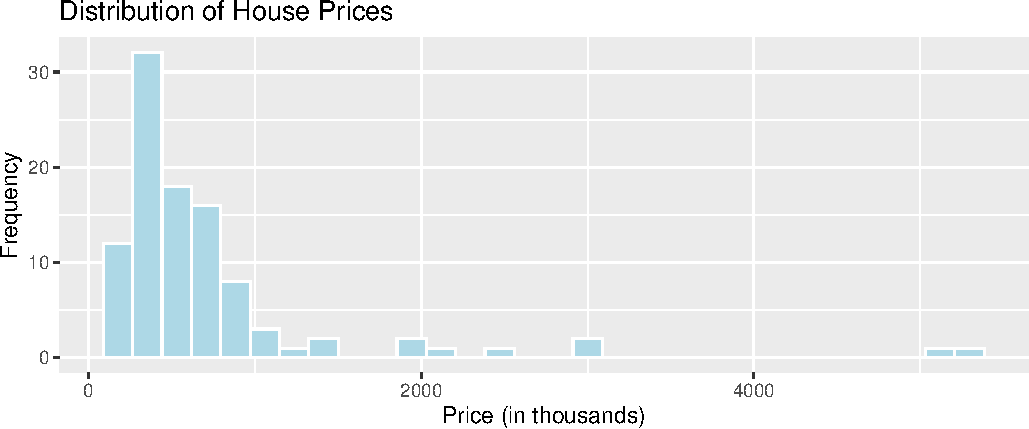
\includegraphics{Ch1_files/figure-pdf/unnamed-chunk-15-1.pdf}

We see that the distribution of house prices is right-skewed. Most
houses cost less than \$1,000,000, though there are a few houses that
are much more expensive. The most common price range is around \$400,000
to \$500,000.

\subsection{Density Plot}\label{density-plot}

Density plots show the distribution for a quantitative variable price.
Scores can be compared across categories, like whether or not the house
is on a waterfront.

\textbf{General Template for Density Plot}

\begin{Shaded}
\begin{Highlighting}[]
\FunctionTok{ggplot}\NormalTok{(}\AttributeTok{data=}\NormalTok{DatasetName, }\FunctionTok{aes}\NormalTok{(}\AttributeTok{x=}\NormalTok{QuantitativeVariable,}
                             \AttributeTok{color=}\NormalTok{CategoricalVariable, }\AttributeTok{fill=}\NormalTok{CategoricalVariable)) }\SpecialCharTok{+} 
  \FunctionTok{geom\_density}\NormalTok{(}\AttributeTok{alpha=}\FloatTok{0.2}\NormalTok{) }\SpecialCharTok{+} 
  \FunctionTok{ggtitle}\NormalTok{(}\StringTok{"Plot Title"}\NormalTok{) }\SpecialCharTok{+}
  \FunctionTok{xlab}\NormalTok{(}\StringTok{"Axis Label"}\NormalTok{) }\SpecialCharTok{+} 
  \FunctionTok{ylab}\NormalTok{(}\StringTok{"Frequency"}\NormalTok{) }
\end{Highlighting}
\end{Shaded}

\texttt{alpha}, ranging from 0 to 1 dictates transparency.

\textbf{Density Plot of House Prices}

\begin{Shaded}
\begin{Highlighting}[]
\FunctionTok{ggplot}\NormalTok{(}\AttributeTok{data=}\NormalTok{Houses, }\FunctionTok{aes}\NormalTok{(}\AttributeTok{x=}\NormalTok{price, }\AttributeTok{color=}\NormalTok{waterfront, }\AttributeTok{fill=}\NormalTok{waterfront)) }\SpecialCharTok{+} 
  \FunctionTok{geom\_density}\NormalTok{(}\AttributeTok{alpha=}\FloatTok{0.2}\NormalTok{) }\SpecialCharTok{+} 
  \FunctionTok{ggtitle}\NormalTok{(}\StringTok{"Distribution of Prices"}\NormalTok{) }\SpecialCharTok{+}
  \FunctionTok{xlab}\NormalTok{(}\StringTok{"House price (in thousands)"}\NormalTok{) }\SpecialCharTok{+} 
  \FunctionTok{ylab}\NormalTok{(}\StringTok{"Frequency"}\NormalTok{) }
\end{Highlighting}
\end{Shaded}

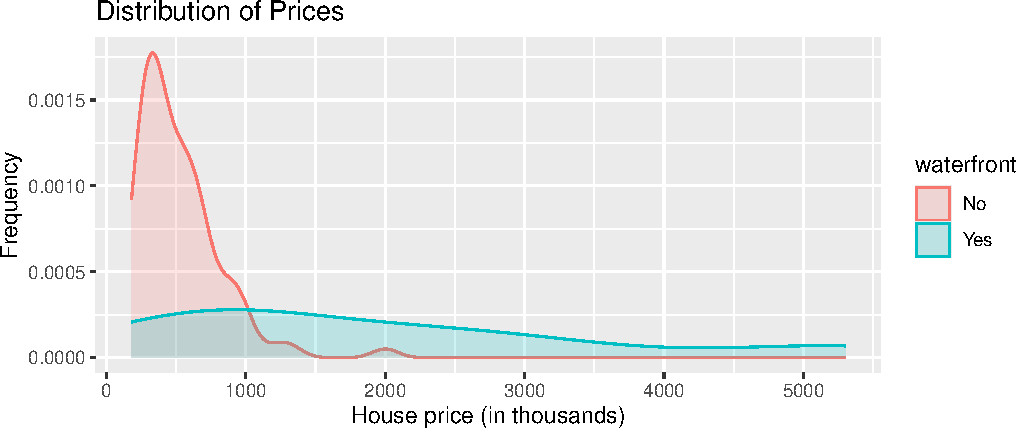
\includegraphics{Ch1_files/figure-pdf/unnamed-chunk-17-1.pdf}

We see that on average, houses on the waterfront tend to be more
expensive and have a greater price range than houses not on the
waterfront.

\subsection{Boxplot}\label{boxplot}

Boxplots can be used to compare a quantitative variable with a
categorical variable. The middle 50\% of observations are contained in
the ``box'', with the upper and lower 25\% of the observations in each
tail.

\textbf{General Template for Boxplot}

\begin{Shaded}
\begin{Highlighting}[]
\FunctionTok{ggplot}\NormalTok{(}\AttributeTok{data=}\NormalTok{DatasetName, }\FunctionTok{aes}\NormalTok{(}\AttributeTok{x=}\NormalTok{CategoricalVariable, }
                             \AttributeTok{y=}\NormalTok{QuantitativeVariable)) }\SpecialCharTok{+} 
  \FunctionTok{geom\_boxplot}\NormalTok{() }\SpecialCharTok{+} 
  \FunctionTok{ggtitle}\NormalTok{(}\StringTok{"Plot Title"}\NormalTok{) }\SpecialCharTok{+} 
  \FunctionTok{xlab}\NormalTok{(}\StringTok{"Variable Name"}\NormalTok{) }\SpecialCharTok{+} \FunctionTok{ylab}\NormalTok{(}\StringTok{"Variable Name"}\NormalTok{) }
\end{Highlighting}
\end{Shaded}

You can make the plot horizontal by adding \texttt{+\ coordflip()}. You
can turn the axis text vertical by adding
\texttt{theme(axis.text.x\ =\ element\_text(angle\ =\ 90))}.

\textbf{Boxplot Comparing Price by Waterfront Status}

\begin{Shaded}
\begin{Highlighting}[]
\FunctionTok{ggplot}\NormalTok{(}\AttributeTok{data=}\NormalTok{Houses, }\FunctionTok{aes}\NormalTok{(}\AttributeTok{x=}\NormalTok{waterfront, }\AttributeTok{y=}\NormalTok{price)) }\SpecialCharTok{+} \FunctionTok{geom\_boxplot}\NormalTok{() }\SpecialCharTok{+} 
  \FunctionTok{ggtitle}\NormalTok{(}\StringTok{"House Price by Waterfront Status"}\NormalTok{) }\SpecialCharTok{+} 
  \FunctionTok{xlab}\NormalTok{(}\StringTok{"Waterfront"}\NormalTok{) }\SpecialCharTok{+} \FunctionTok{ylab}\NormalTok{(}\StringTok{"Price (in thousands)"}\NormalTok{) }\SpecialCharTok{+} \FunctionTok{coord\_flip}\NormalTok{()}
\end{Highlighting}
\end{Shaded}

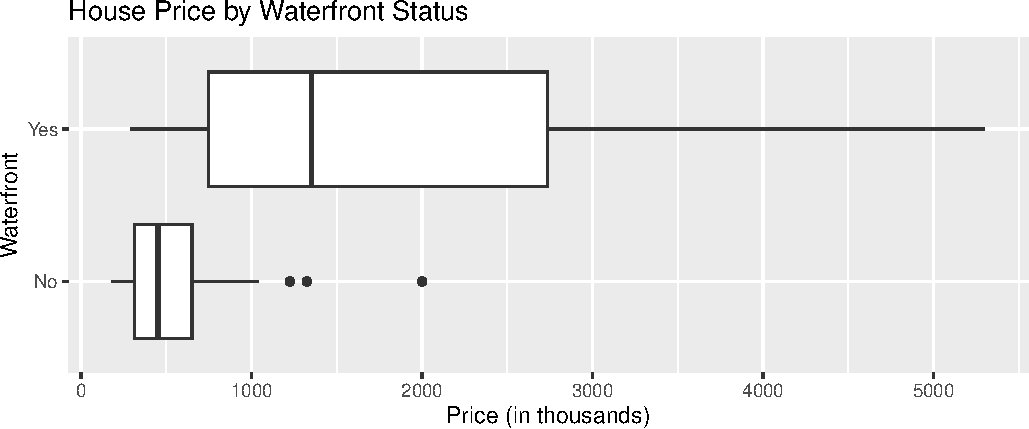
\includegraphics{Ch1_files/figure-pdf/unnamed-chunk-19-1.pdf}

For houses not on the waterfront, the median price is about \$400,000,
and the middle 50\% of prices range from about \$300,000 to \$600,000.

For waterfront houses, the median price is about \$1,500,000, and the
middle 50\% of prices range from about \$900,000 to \$1,900,000.

\subsection{Violin Plot}\label{violin-plot}

Violin plots are an alternative to boxplots. The width of the violin
tells us the density of observations in a given range.

\textbf{General Template for Violin Plot}

\begin{Shaded}
\begin{Highlighting}[]
\FunctionTok{ggplot}\NormalTok{(}\AttributeTok{data=}\NormalTok{DatasetName, }\FunctionTok{aes}\NormalTok{(}\AttributeTok{x=}\NormalTok{CategoricalVariable, }\AttributeTok{y=}\NormalTok{QuantitativeVariable, }
                             \AttributeTok{fill=}\NormalTok{CategoricalVariable)) }\SpecialCharTok{+} 
  \FunctionTok{geom\_violin}\NormalTok{() }\SpecialCharTok{+} 
  \FunctionTok{ggtitle}\NormalTok{(}\StringTok{"Plot Title"}\NormalTok{) }\SpecialCharTok{+} 
  \FunctionTok{xlab}\NormalTok{(}\StringTok{"Variable Name"}\NormalTok{) }\SpecialCharTok{+} \FunctionTok{ylab}\NormalTok{(}\StringTok{"Variable Name"}\NormalTok{) }
\end{Highlighting}
\end{Shaded}

\textbf{Violin Plot Comparing Prices by Waterfront}

\begin{Shaded}
\begin{Highlighting}[]
\FunctionTok{ggplot}\NormalTok{(}\AttributeTok{data=}\NormalTok{Houses, }\FunctionTok{aes}\NormalTok{(}\AttributeTok{x=}\NormalTok{waterfront, }\AttributeTok{y=}\NormalTok{price, }\AttributeTok{fill=}\NormalTok{waterfront)) }\SpecialCharTok{+} 
  \FunctionTok{geom\_violin}\NormalTok{() }\SpecialCharTok{+} 
  \FunctionTok{ggtitle}\NormalTok{(}\StringTok{"Price by Waterfront Status"}\NormalTok{) }\SpecialCharTok{+} 
  \FunctionTok{xlab}\NormalTok{(}\StringTok{"Waterfront"}\NormalTok{) }\SpecialCharTok{+} \FunctionTok{ylab}\NormalTok{(}\StringTok{"Price (in thousands)"}\NormalTok{) }\SpecialCharTok{+} 
  \FunctionTok{theme}\NormalTok{(}\AttributeTok{axis.text.x =} \FunctionTok{element\_text}\NormalTok{(}\AttributeTok{angle =} \DecValTok{90}\NormalTok{))}
\end{Highlighting}
\end{Shaded}

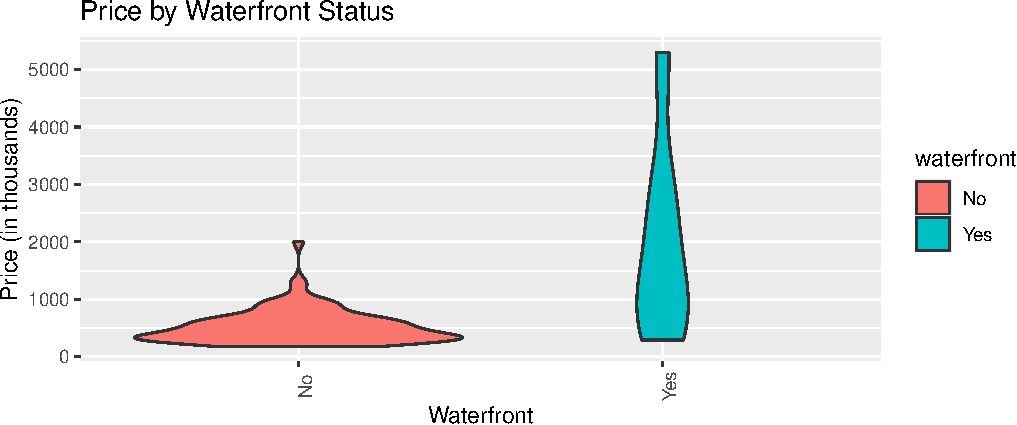
\includegraphics{Ch1_files/figure-pdf/unnamed-chunk-21-1.pdf}

Again, we see that houses on the waterfront tend to be more expensive
than those not on the waterfront, and have a wider range in prices.

\subsection{Scatterplot}\label{scatterplot}

Scatterplots are used to visualize the relationship between two
quantitative variables.

\textbf{Scatterplot Template}

\begin{Shaded}
\begin{Highlighting}[]
\FunctionTok{ggplot}\NormalTok{(}\AttributeTok{data=}\NormalTok{DatasetName, }\FunctionTok{aes}\NormalTok{(}\AttributeTok{x=}\NormalTok{CategoricalVariable, }\AttributeTok{y=}\NormalTok{QuantitativeVariable)) }\SpecialCharTok{+} 
  \FunctionTok{geom\_point}\NormalTok{() }\SpecialCharTok{+}
  \FunctionTok{ggtitle}\NormalTok{(}\StringTok{"Plot Title"}\NormalTok{) }\SpecialCharTok{+} 
  \FunctionTok{ylab}\NormalTok{(}\StringTok{"Axis Label"}\NormalTok{) }\SpecialCharTok{+} 
  \FunctionTok{xlab}\NormalTok{(}\StringTok{"Axis Label"}\NormalTok{)}
\end{Highlighting}
\end{Shaded}

\textbf{Scatterplot Comparing Price and Square Feet of Living Space}

\begin{Shaded}
\begin{Highlighting}[]
\FunctionTok{ggplot}\NormalTok{(}\AttributeTok{data=}\NormalTok{Houses, }\FunctionTok{aes}\NormalTok{(}\AttributeTok{x=}\NormalTok{sqft\_living, }\AttributeTok{y=}\NormalTok{price)) }\SpecialCharTok{+} 
  \FunctionTok{geom\_point}\NormalTok{() }\SpecialCharTok{+}
  \FunctionTok{ggtitle}\NormalTok{(}\StringTok{"Price and Living Space"}\NormalTok{) }\SpecialCharTok{+} 
  \FunctionTok{ylab}\NormalTok{(}\StringTok{"Price (in thousands)"}\NormalTok{) }\SpecialCharTok{+} 
  \FunctionTok{xlab}\NormalTok{(}\StringTok{"Living Space in sq. ft. "}\NormalTok{)}
\end{Highlighting}
\end{Shaded}

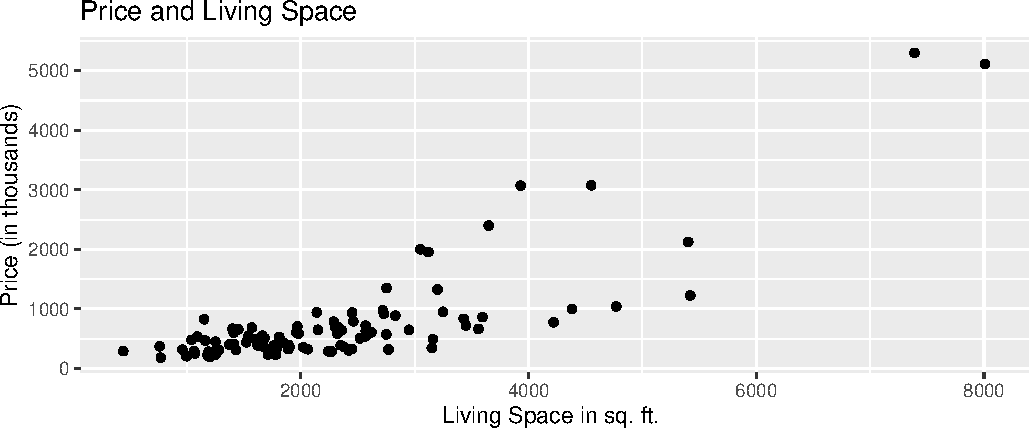
\includegraphics{Ch1_files/figure-pdf/unnamed-chunk-23-1.pdf}

We see that there is an upward trend, indicating that houses with more
living space tend to, on average, be higher priced than those with less
living space. The relationship appears to be roughly linear, though
there might be some curvature, as living space gets very large. There
are some exceptions to this trend, most notably a house with more than
7,000 square feet, priced just over \$1,000,000.

We can also add color, size, and shape to the scatterplot to display
information about other variables.

We'll use color to illustrate whether the house is on the waterfront,
and size to represent the square footage of the entire lot (including
the yard and the house).

\begin{Shaded}
\begin{Highlighting}[]
\FunctionTok{ggplot}\NormalTok{(}\AttributeTok{data=}\NormalTok{Houses, }
       \FunctionTok{aes}\NormalTok{(}\AttributeTok{x=}\NormalTok{sqft\_living, }\AttributeTok{y=}\NormalTok{price, }\AttributeTok{color=}\NormalTok{waterfront, }\AttributeTok{size=}\NormalTok{sqft\_lot)) }\SpecialCharTok{+} 
  \FunctionTok{geom\_point}\NormalTok{() }\SpecialCharTok{+}
  \FunctionTok{ggtitle}\NormalTok{(}\StringTok{"Price of King County Houses"}\NormalTok{) }\SpecialCharTok{+} 
  \FunctionTok{ylab}\NormalTok{(}\StringTok{"Price (in thousands)"}\NormalTok{) }\SpecialCharTok{+} 
  \FunctionTok{xlab}\NormalTok{(}\StringTok{"Living Space in sq. ft. "}\NormalTok{)}
\end{Highlighting}
\end{Shaded}

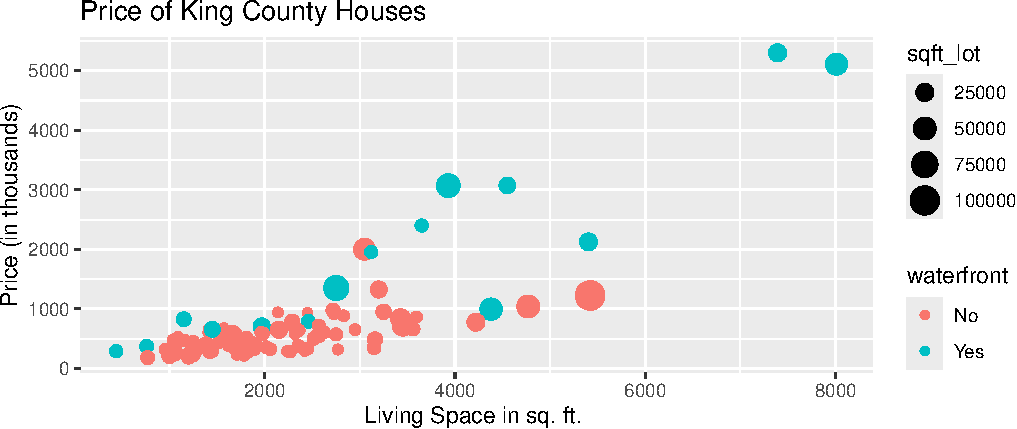
\includegraphics{Ch1_files/figure-pdf/unnamed-chunk-24-1.pdf}

We notice that many of the largest and most expensive houses are on the
waterfront.

\subsection{Bar Graph}\label{bar-graph}

Bar graphs can be used to visualize one or more categorical variables. A
bar graph is similar to a histogram, in that the y-axis again displays
frequency, but the x-axis displays categories, instead of ranges of
values.

\textbf{Bar Graph Template}

\begin{Shaded}
\begin{Highlighting}[]
\FunctionTok{ggplot}\NormalTok{(}\AttributeTok{data=}\NormalTok{DatasetName, }\FunctionTok{aes}\NormalTok{(}\AttributeTok{x=}\NormalTok{CategoricalVariable)) }\SpecialCharTok{+} 
  \FunctionTok{geom\_bar}\NormalTok{(}\AttributeTok{fill=}\StringTok{"colorchoice"}\NormalTok{,}\AttributeTok{color=}\StringTok{"colorchoice"}\NormalTok{)  }\SpecialCharTok{+} 
  \FunctionTok{ggtitle}\NormalTok{(}\StringTok{"Plot Title"}\NormalTok{) }\SpecialCharTok{+} 
  \FunctionTok{xlab}\NormalTok{(}\StringTok{"Variable Name"}\NormalTok{) }\SpecialCharTok{+} 
  \FunctionTok{ylab}\NormalTok{(}\StringTok{"Frequency"}\NormalTok{) }
\end{Highlighting}
\end{Shaded}

\textbf{Bar Graph by Condition}

\begin{Shaded}
\begin{Highlighting}[]
\FunctionTok{ggplot}\NormalTok{(}\AttributeTok{data=}\NormalTok{Houses, }\FunctionTok{aes}\NormalTok{(}\AttributeTok{x=}\NormalTok{condition)) }\SpecialCharTok{+} 
  \FunctionTok{geom\_bar}\NormalTok{(}\AttributeTok{fill=}\StringTok{"lightblue"}\NormalTok{,}\AttributeTok{color=}\StringTok{"white"}\NormalTok{)  }\SpecialCharTok{+} 
  \FunctionTok{ggtitle}\NormalTok{(}\StringTok{"Number of Houses by Condition"}\NormalTok{) }\SpecialCharTok{+} 
  \FunctionTok{xlab}\NormalTok{(}\StringTok{"Condition"}\NormalTok{) }\SpecialCharTok{+} 
  \FunctionTok{ylab}\NormalTok{(}\StringTok{"Frequency"}\NormalTok{) }\SpecialCharTok{+}   
  \FunctionTok{theme}\NormalTok{(}\AttributeTok{axis.text.x =} \FunctionTok{element\_text}\NormalTok{(}\AttributeTok{angle =} \DecValTok{90}\NormalTok{))}
\end{Highlighting}
\end{Shaded}

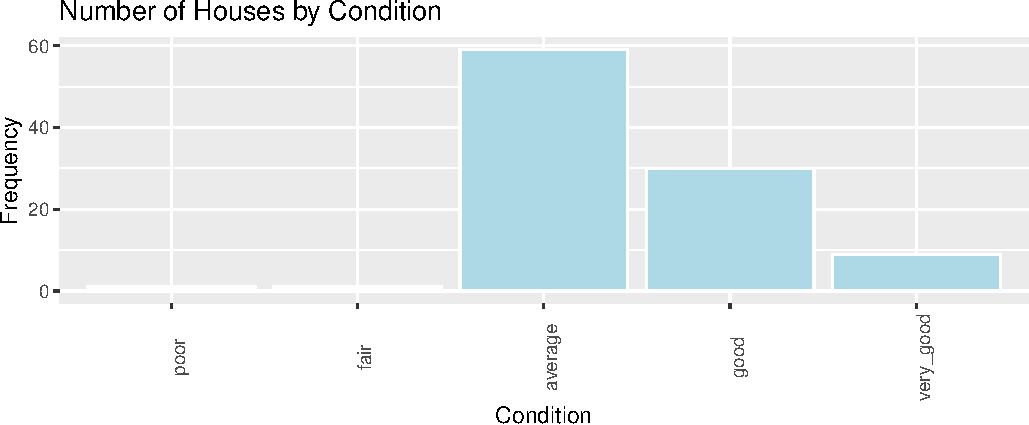
\includegraphics{Ch1_files/figure-pdf/unnamed-chunk-26-1.pdf}

We see that the majority of houses are in average condition. Some are in
good or very good condition, while very few are in poor or very poor
condition.

\subsection{Stacked and Side-by-Side Bar
Graphs}\label{stacked-and-side-by-side-bar-graphs}

\textbf{Stacked Bar Graph Template}

\begin{Shaded}
\begin{Highlighting}[]
\FunctionTok{ggplot}\NormalTok{(}\AttributeTok{data =}\NormalTok{ DatasetName, }\AttributeTok{mapping =} \FunctionTok{aes}\NormalTok{(}\AttributeTok{x =}\NormalTok{ CategoricalVariable1, }
                                         \AttributeTok{fill =}\NormalTok{ CategoricalVariable2)) }\SpecialCharTok{+}
    \FunctionTok{stat\_count}\NormalTok{(}\AttributeTok{position=}\StringTok{"fill"}\NormalTok{)  }\SpecialCharTok{+}
  \FunctionTok{theme\_bw}\NormalTok{() }\SpecialCharTok{+} \FunctionTok{ggtitle}\NormalTok{(}\StringTok{"Plot Title"}\NormalTok{) }\SpecialCharTok{+} 
  \FunctionTok{xlab}\NormalTok{(}\StringTok{"Variable 1"}\NormalTok{) }\SpecialCharTok{+} 
  \FunctionTok{ylab}\NormalTok{(}\StringTok{"Proportion of Variable 2"}\NormalTok{) }\SpecialCharTok{+}   
  \FunctionTok{theme}\NormalTok{(}\AttributeTok{axis.text.x =} \FunctionTok{element\_text}\NormalTok{(}\AttributeTok{angle =} \DecValTok{90}\NormalTok{)) }
\end{Highlighting}
\end{Shaded}

\textbf{Stacked Bar Graph Example}

The \texttt{stat\_count(position="fill")} command creates a stacked bar
graph, comparing two categorical variables. Let's explore whether
waterfront status is related to condition.

\begin{Shaded}
\begin{Highlighting}[]
\FunctionTok{ggplot}\NormalTok{(}\AttributeTok{data =}\NormalTok{ Houses, }\AttributeTok{mapping =} \FunctionTok{aes}\NormalTok{(}\AttributeTok{x =}\NormalTok{ waterfront, }\AttributeTok{fill =}\NormalTok{ condition)) }\SpecialCharTok{+}
    \FunctionTok{stat\_count}\NormalTok{(}\AttributeTok{position=}\StringTok{"fill"}\NormalTok{)  }\SpecialCharTok{+}
  \FunctionTok{theme\_bw}\NormalTok{() }\SpecialCharTok{+} \FunctionTok{ggtitle}\NormalTok{(}\StringTok{"Condition by Waterfront Status"}\NormalTok{) }\SpecialCharTok{+} 
  \FunctionTok{xlab}\NormalTok{(}\StringTok{"Waterfront Status"}\NormalTok{) }\SpecialCharTok{+} 
  \FunctionTok{ylab}\NormalTok{(}\StringTok{"Condition"}\NormalTok{) }\SpecialCharTok{+}   
  \FunctionTok{theme}\NormalTok{(}\AttributeTok{axis.text.x =} \FunctionTok{element\_text}\NormalTok{(}\AttributeTok{angle =} \DecValTok{90}\NormalTok{)) }
\end{Highlighting}
\end{Shaded}

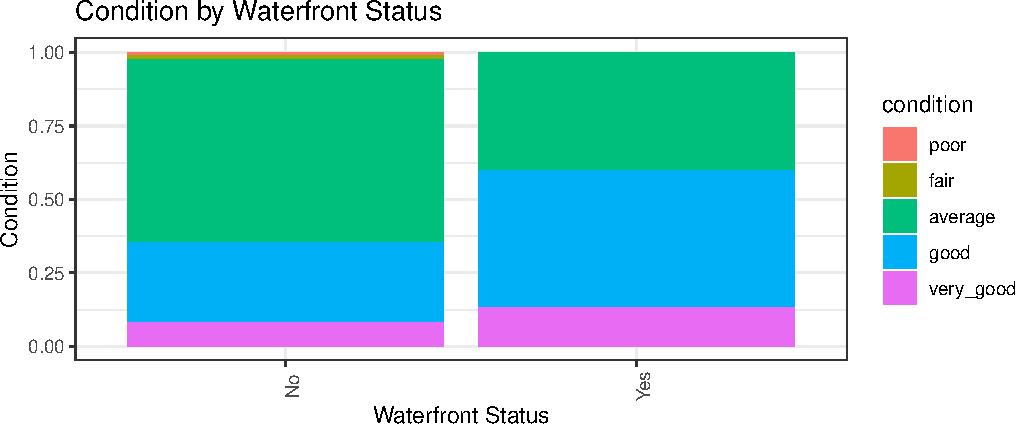
\includegraphics{Ch1_files/figure-pdf/unnamed-chunk-28-1.pdf}

We see that a higher proportion of waterfront houses are in good or
excellent condition than non-waterfront houses.

\textbf{Side-by-side Bar Graph Template}

We can create a side-by-side bar graph, using \texttt{position=dodge}.

\begin{Shaded}
\begin{Highlighting}[]
\FunctionTok{ggplot}\NormalTok{(}\AttributeTok{data =}\NormalTok{ DatasetName, }\AttributeTok{mapping =} \FunctionTok{aes}\NormalTok{(}\AttributeTok{x =}\NormalTok{ CategoricalVariable1, }
                                         \AttributeTok{fill =}\NormalTok{ CategoricalVariable2)) }\SpecialCharTok{+}
    \FunctionTok{geom\_bar}\NormalTok{(}\AttributeTok{position =} \StringTok{"dodge"}\NormalTok{) }\SpecialCharTok{+}
  \FunctionTok{ggtitle}\NormalTok{(}\StringTok{"Plot Title"}\NormalTok{) }\SpecialCharTok{+} 
  \FunctionTok{xlab}\NormalTok{(}\StringTok{"Genre"}\NormalTok{) }\SpecialCharTok{+} 
  \FunctionTok{ylab}\NormalTok{(}\StringTok{"Frequency"}\NormalTok{) }
\end{Highlighting}
\end{Shaded}

\textbf{Side-by-side Bar Graph Example}

\begin{Shaded}
\begin{Highlighting}[]
\FunctionTok{ggplot}\NormalTok{(}\AttributeTok{data =}\NormalTok{ Houses, }\AttributeTok{mapping =} \FunctionTok{aes}\NormalTok{(}\AttributeTok{x =}\NormalTok{ waterfront, }\AttributeTok{fill =}\NormalTok{ condition)) }\SpecialCharTok{+}
    \FunctionTok{geom\_bar}\NormalTok{(}\AttributeTok{position =} \StringTok{"dodge"}\NormalTok{) }\SpecialCharTok{+}
  \FunctionTok{ggtitle}\NormalTok{(}\StringTok{"Condition by Waterfront Status"}\NormalTok{) }\SpecialCharTok{+} 
  \FunctionTok{xlab}\NormalTok{(}\StringTok{"Waterfront Status"}\NormalTok{) }\SpecialCharTok{+} 
  \FunctionTok{ylab}\NormalTok{(}\StringTok{"Condition"}\NormalTok{) }\SpecialCharTok{+}   
  \FunctionTok{theme}\NormalTok{(}\AttributeTok{axis.text.x =} \FunctionTok{element\_text}\NormalTok{(}\AttributeTok{angle =} \DecValTok{90}\NormalTok{)) }
\end{Highlighting}
\end{Shaded}

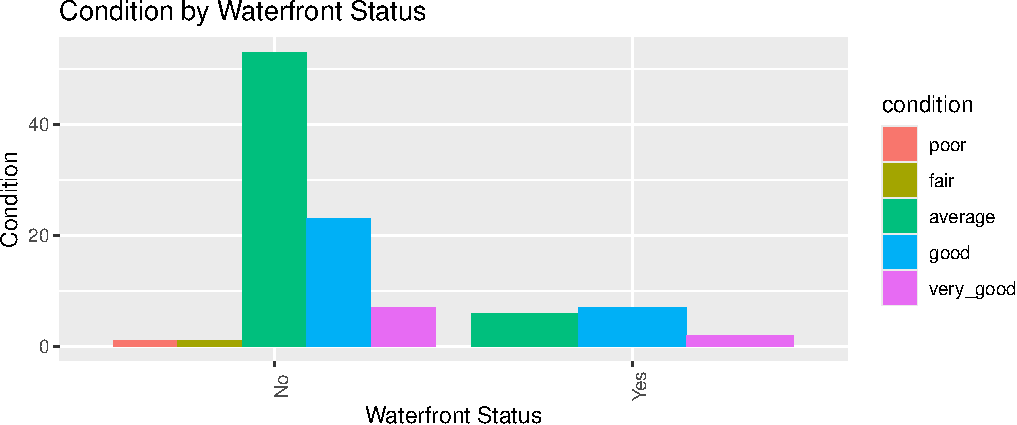
\includegraphics{Ch1_files/figure-pdf/unnamed-chunk-30-1.pdf}

In this case, since there are so few waterfront houses, the graph is
hard to read and not very useful.

The stacked bar graph is a better way to convey information in this
instance, though you may find that for a different dataset, the
side-by-side bar graph could be a better choice.

\subsection{Correlation Plot}\label{correlation-plot}

Correlation plots can be used to visualize relationships between
quantitative variables. Correlation is a number between -1 and 1,
describing the strength of the linear relationship between two
variables. Variables with strong positive correlations will have
correlation close to +1, while variables with strong negative
correlations will have correlations close to -1. Variables with little
to no relationship will have correlation close to 0.

The \texttt{cor()} function calculates correlations between quantitative
variables. We'll use \texttt{select\_if} to select only numeric
variables. The `use=``complete.obs'' command tells R to ignore
observations with missing data.

\begin{Shaded}
\begin{Highlighting}[]
\FunctionTok{cor}\NormalTok{(}\FunctionTok{select\_if}\NormalTok{(Houses, is.numeric), }\AttributeTok{use=}\StringTok{"complete.obs"}\NormalTok{) }\SpecialCharTok{|\textgreater{}} \FunctionTok{round}\NormalTok{(}\DecValTok{2}\NormalTok{)}
\end{Highlighting}
\end{Shaded}

\begin{verbatim}
               Id price bedrooms bathrooms sqft_living sqft_lot yr_built   age
Id           1.00  0.03    -0.06     -0.01       -0.03    -0.07    -0.02  0.02
price        0.03  1.00     0.40      0.67        0.81     0.42     0.17 -0.17
bedrooms    -0.06  0.40     1.00      0.58        0.58     0.15     0.26 -0.26
bathrooms   -0.01  0.67     0.58      1.00        0.85     0.45     0.50 -0.50
sqft_living -0.03  0.81     0.58      0.85        1.00     0.54     0.36 -0.36
sqft_lot    -0.07  0.42     0.15      0.45        0.54     1.00     0.14 -0.14
yr_built    -0.02  0.17     0.26      0.50        0.36     0.14     1.00 -1.00
age          0.02 -0.17    -0.26     -0.50       -0.36    -0.14    -1.00  1.00
\end{verbatim}

The \texttt{corrplot()} function in the \texttt{corrplot()} package
provides a visualization of the correlations. Larger, thicker circles
indicate stronger correlations.

\begin{Shaded}
\begin{Highlighting}[]
\FunctionTok{library}\NormalTok{(corrplot)}
\NormalTok{Corr }\OtherTok{\textless{}{-}} \FunctionTok{cor}\NormalTok{(}\FunctionTok{select\_if}\NormalTok{(Houses, is.numeric), }\AttributeTok{use=}\StringTok{"complete.obs"}\NormalTok{)}
\FunctionTok{corrplot}\NormalTok{(Corr)}
\end{Highlighting}
\end{Shaded}

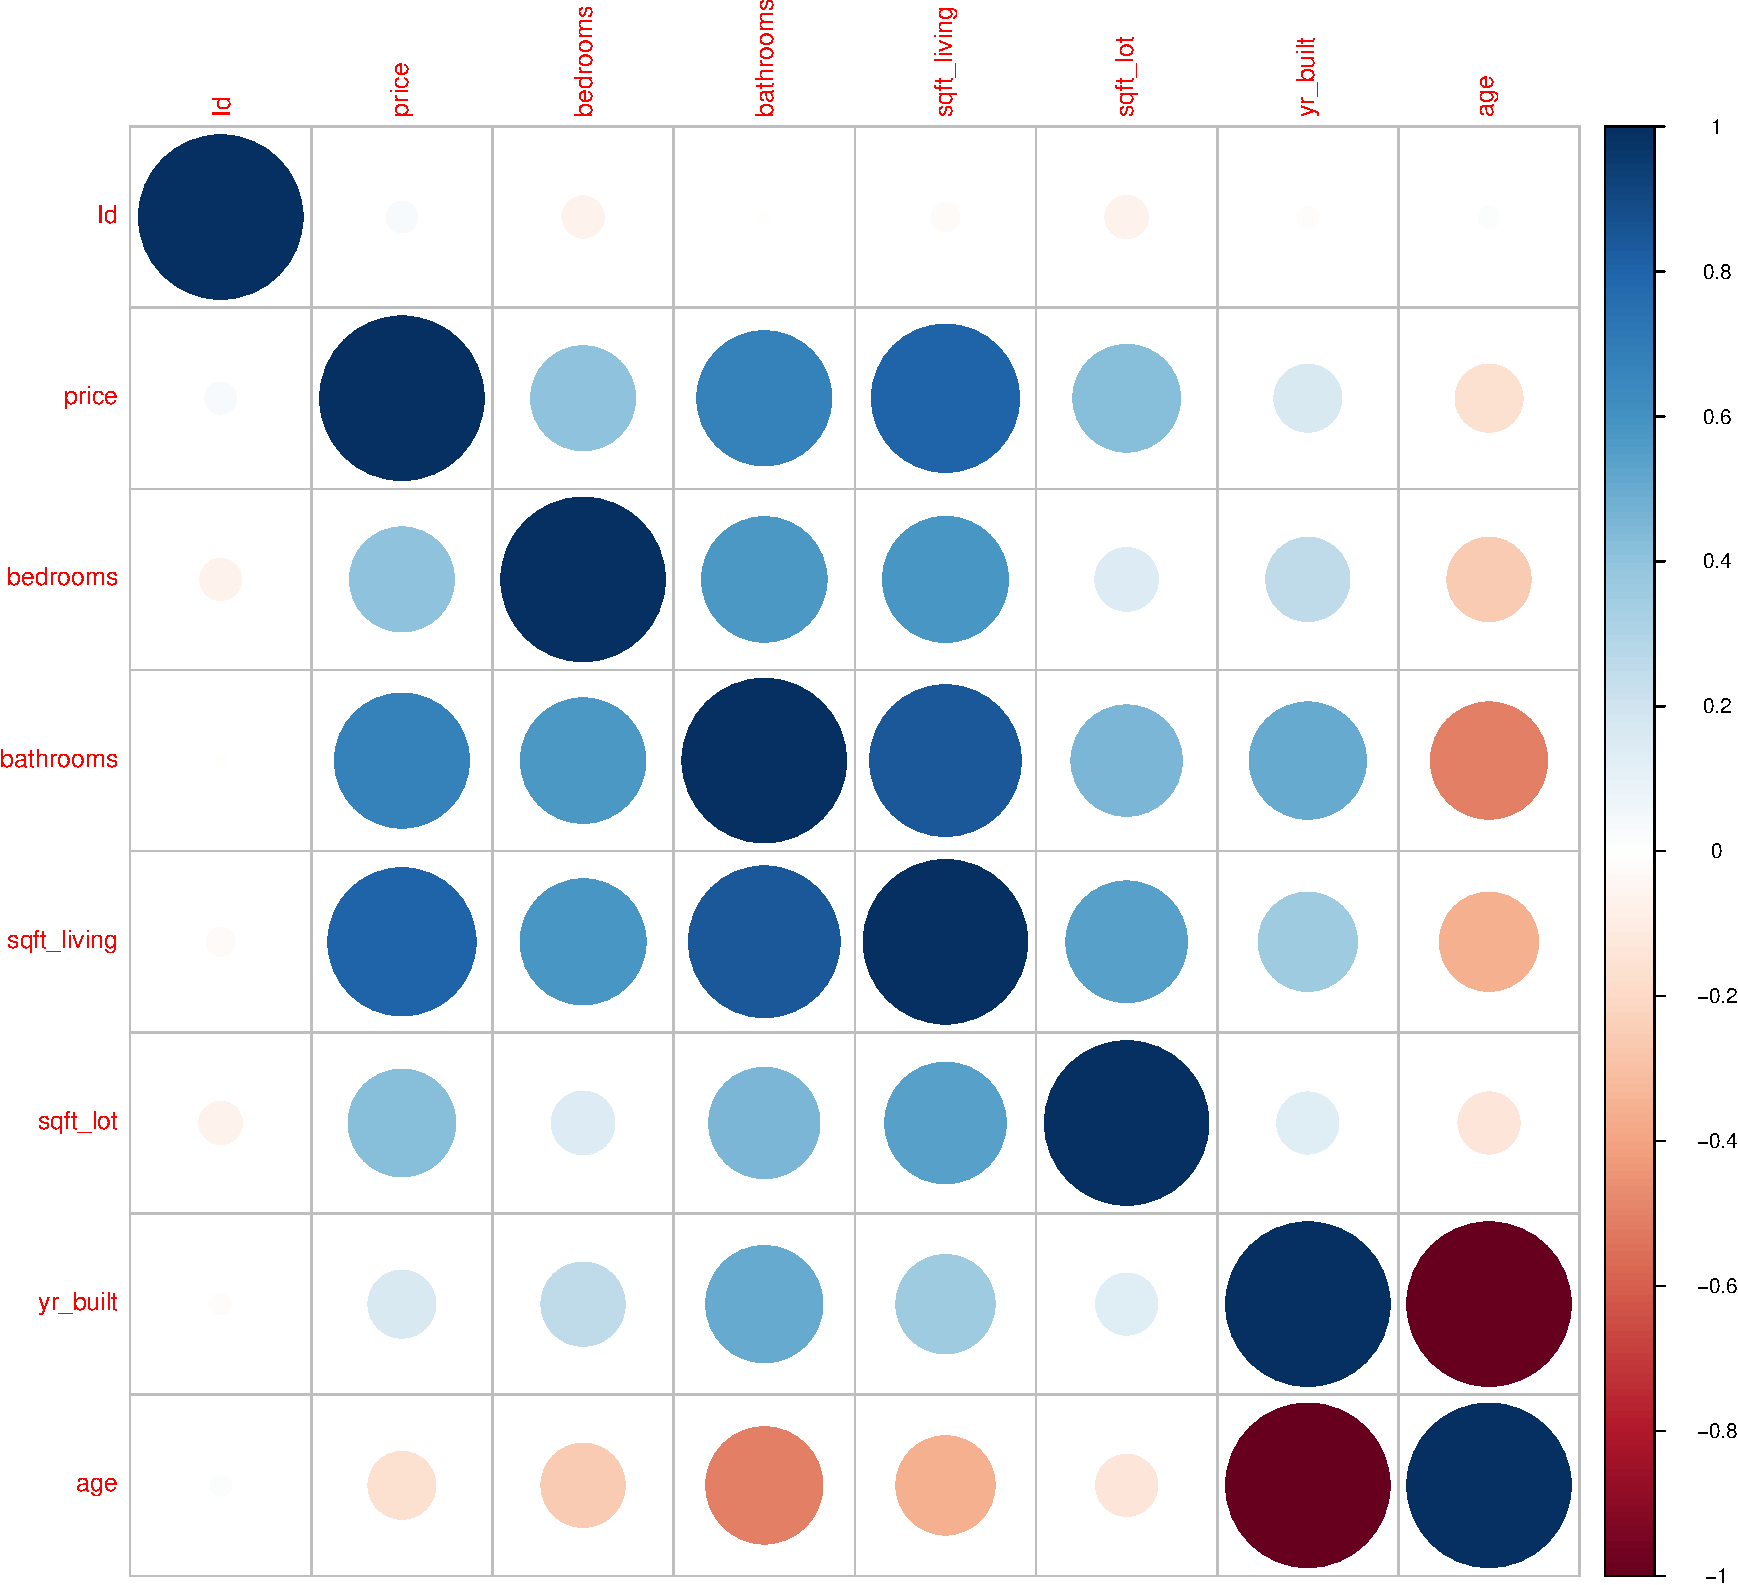
\includegraphics{Ch1_files/figure-pdf/unnamed-chunk-32-1.pdf}

We see that price has a strong positive correlation with square feet of
living space, and is also positively correlated with number of bedrooms
and bathrooms. Living space, bedrooms, and bathrooms are all positively
correlated, which makes sense, since we would expect bigger houses to
have more bedrooms and bathrooms. Price does not show much correlation
with the other variables. We notice that bathrooms is negatively
correlated with age, which means older houses tend to have fewer
bathrooms than newer ones. Not surprisingly, age is very strongly
correlated with year built.

\subsection{Scatterplot Matrix}\label{scatterplot-matrix}

A scatterplot matrix is a grid of plots. It can be created using the
\texttt{ggpairs()} function in the \texttt{GGally} package.

The scatterplot matrix shows us:

\begin{enumerate}
\def\labelenumi{\arabic{enumi}.}
\tightlist
\item
  Along the diagonal are density plots for quantitative variables, or
  bar graphs for categorical variables, showing the distribution of each
  variable.\\
\item
  Under the diagonal are plots showing the relationships between the
  variables in the corresponding row and column. Scatterplots are used
  when both variables are quantitative, bar graphs are used when both
  variables are categorical, and boxplots are used when one variable is
  categorical, and the other is quantitative.\\
\item
  Above the diagonal are correlations between quantitative variables.
\end{enumerate}

Including too many variables can make these hard to read, so it's a good
idea to use \texttt{select} to narrow down the number of variables.

\begin{Shaded}
\begin{Highlighting}[]
\FunctionTok{library}\NormalTok{(GGally)}
\FunctionTok{ggpairs}\NormalTok{(Houses }\SpecialCharTok{|\textgreater{}} \FunctionTok{select}\NormalTok{(price, sqft\_living, condition, age))}
\end{Highlighting}
\end{Shaded}

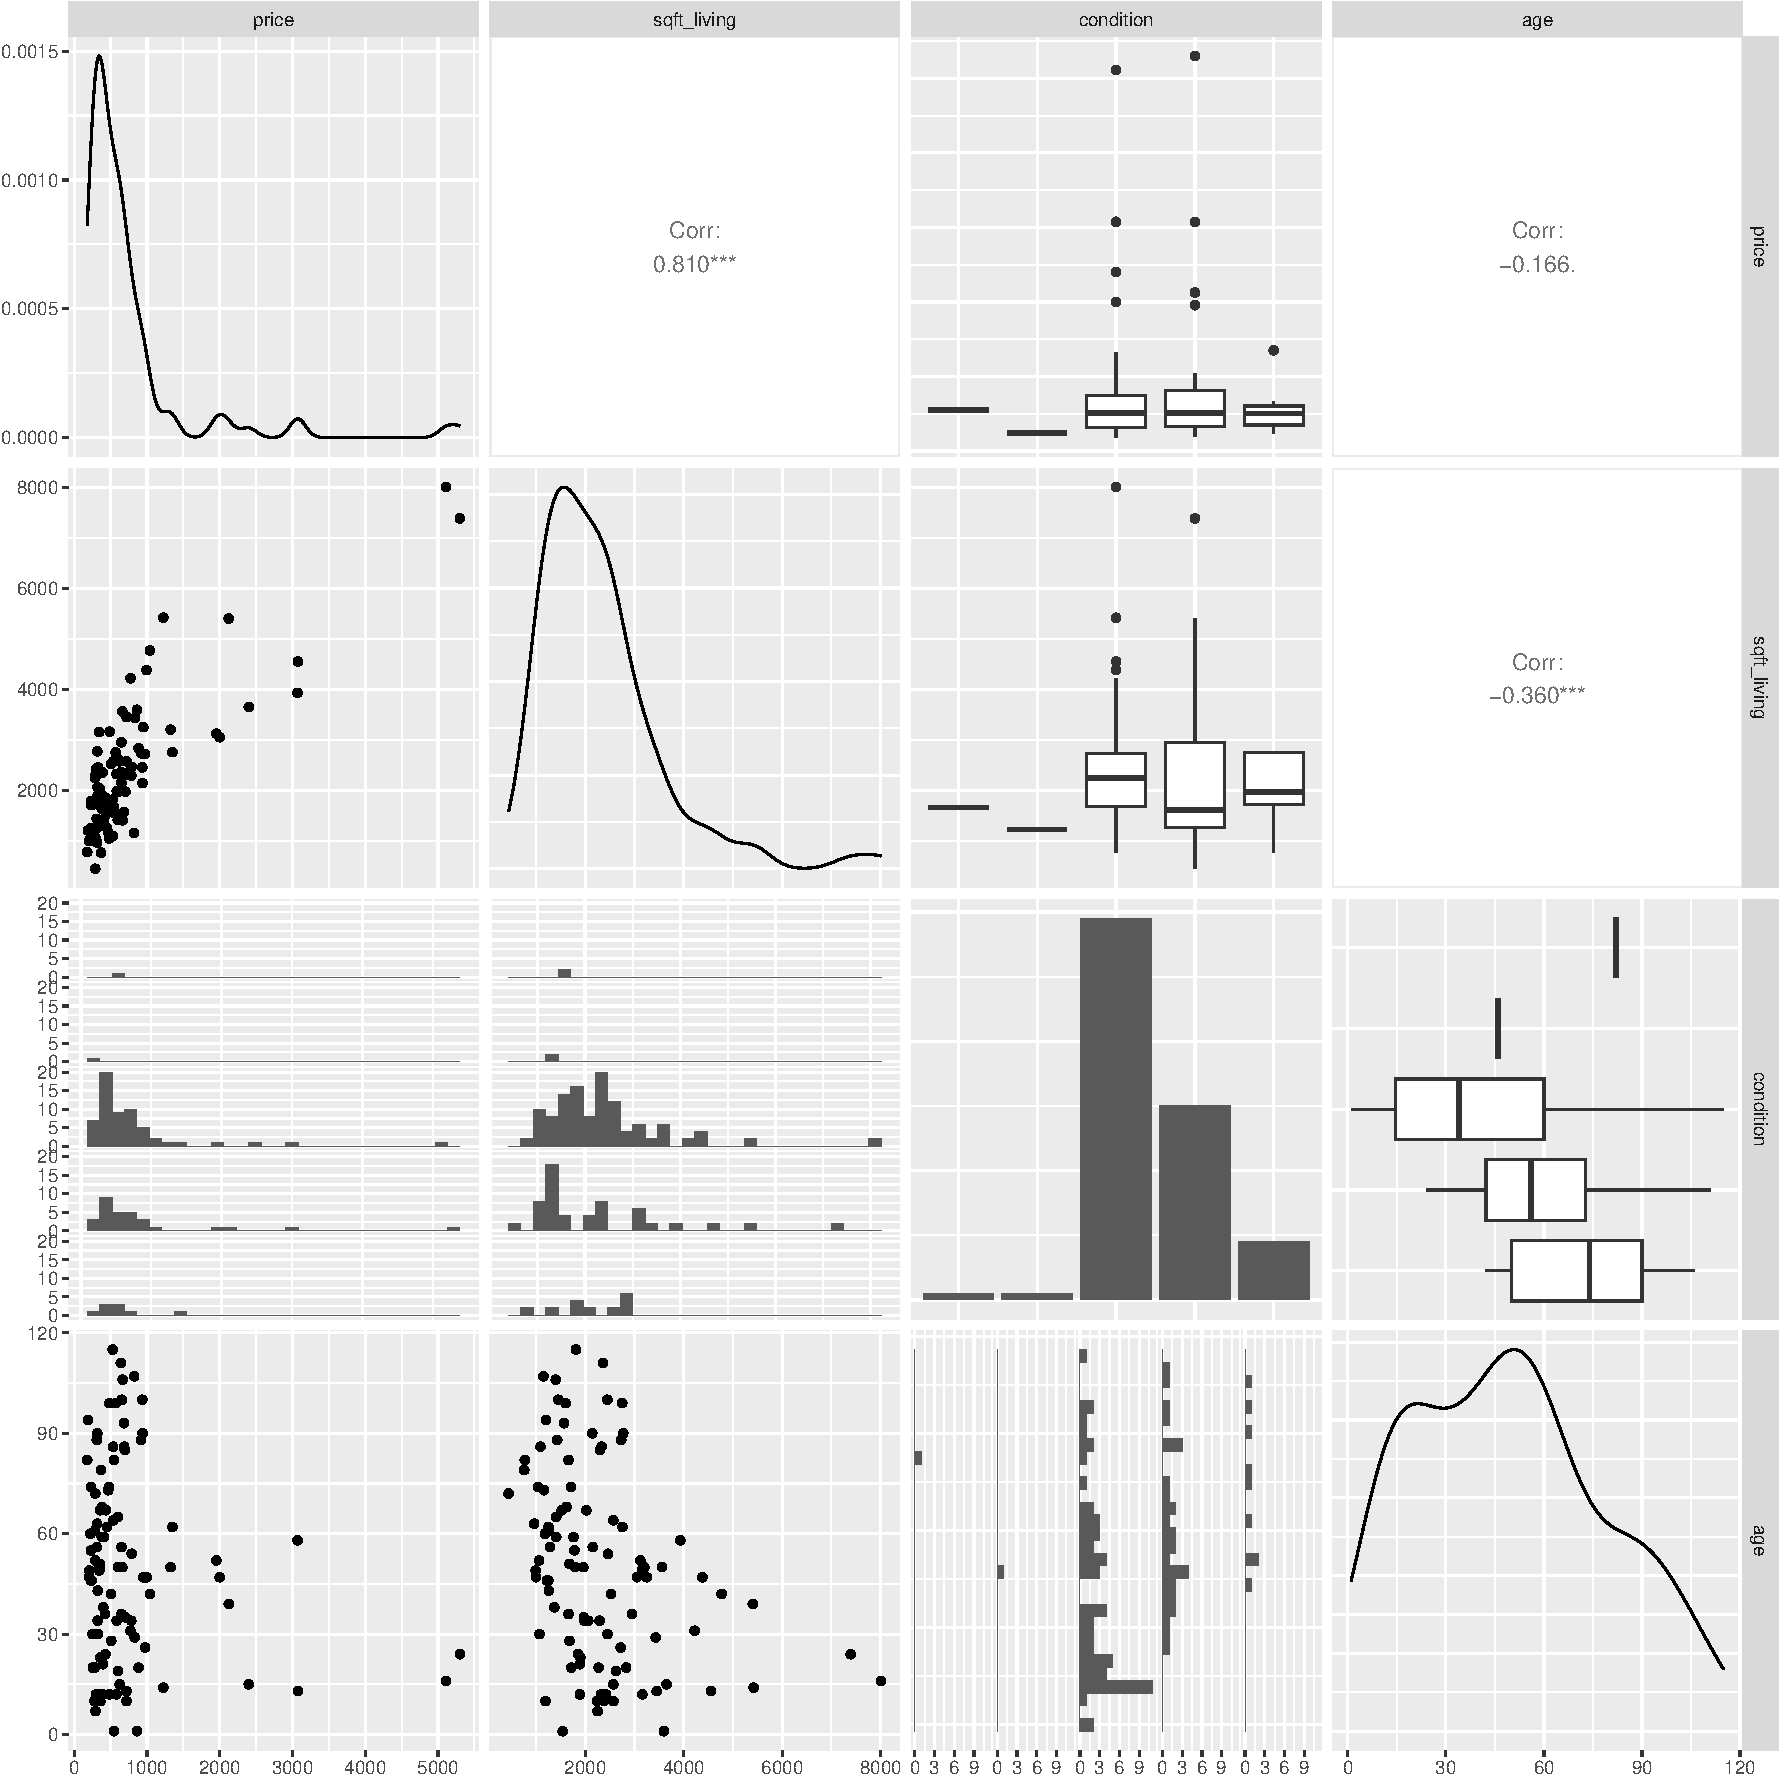
\includegraphics{Ch1_files/figure-pdf/unnamed-chunk-33-1.pdf}

The scatterplot matrix is useful for helping us notice key trends in our
data. However, the plot can hard to read as it is quite dense,
especially when there are a large number of variables. These can help us
look for trends from a distance, but we should then focus in on more
specific plots.

\bookmarksetup{startatroot}

\chapter{Introduction to Statistical
Models}\label{introduction-to-statistical-models}

\textbf{Learning Outcomes:}

\begin{enumerate}
\def\labelenumi{\arabic{enumi}.}
\setcounter{enumi}{4}
\tightlist
\item
  Use regression models to calculate predicted values, changes, and
  differences.\\
\item
  Interpret regression coefficients for simple linear and multiple
  regression models, including models with interaction.\\
\item
  Calculate and interpret regression sums of squares SSR, SSM, and SST,
  and coefficient of determination,\(R^2\).\\
\item
  Determine how changes to sample size, number of terms in a model, or
  regression coefficients impact SST, SSR, and \(R^2\).\\
\item
  Explain what interactions between variables mean, in context.\\
\item
  Explain the least-squares estimation process.\\
\item
  Show how to calculate F-statistics.\\
\item
  Draw conclusions based on F-statistics.\\
\item
  Fit regression models using R and report conclusions.
\end{enumerate}

\section{Fitting Models to Data}\label{fitting-models-to-data}

\subsection{Terminology}\label{terminology}

In this section, we'll use statistical models to predict the prices of
houses in King County, WA.

In a statistical model,

\begin{itemize}
\item
  The variable we are trying to predict (price) is called the
  \textbf{response variable} (denoted \(Y\)).
\item
  Variable(s) we use to help us make the prediction is(are) called
  \textbf{explanatory variables} (denoted \(X\)). These are also
  referred to as \textbf{predictor variables} or \textbf{covariates}.
\end{itemize}

In this section, we'll attempt to predict the price of a house, using
information about its size (in square feet), and whether or not it is on
the waterfront. The price is our response variable, while size and
waterfront location are explanatory variables.

\begin{itemize}
\item
  \textbf{Categorical variables} are variables that take on groups or
  categories, rather than numeric values, for example, whether or not
  the house is on the waterfront.
\item
  \textbf{Quantitative variables} take on meaningful numeric values, for
  example the number of square feet in the house.
\end{itemize}

\subsection{Quantitative Explanatory
Variable}\label{quantitative-explanatory-variable}

We'll first predict the price of the house, using the number of square
feet of living space as our explanatory variable.

We'll assume that price changes linearly with square feet, and fit a
trend line to the data.

\begin{Shaded}
\begin{Highlighting}[]
\FunctionTok{ggplot}\NormalTok{(}\AttributeTok{data=}\NormalTok{Houses, }\FunctionTok{aes}\NormalTok{(}\AttributeTok{x=}\NormalTok{sqft\_living, }\AttributeTok{y=}\NormalTok{price)) }\SpecialCharTok{+}
  \FunctionTok{geom\_point}\NormalTok{() }\SpecialCharTok{+}
  \FunctionTok{stat\_smooth}\NormalTok{(}\AttributeTok{method=}\StringTok{"lm"}\NormalTok{, }\AttributeTok{se=}\ConstantTok{FALSE}\NormalTok{) }\SpecialCharTok{+}
  \FunctionTok{ggtitle}\NormalTok{(}\StringTok{"Price and Living Space"}\NormalTok{) }\SpecialCharTok{+} 
  \FunctionTok{ylab}\NormalTok{(}\StringTok{"Price"}\NormalTok{) }\SpecialCharTok{+} 
  \FunctionTok{xlab}\NormalTok{(}\StringTok{"Living Space in sq. ft. "}\NormalTok{)}
\end{Highlighting}
\end{Shaded}

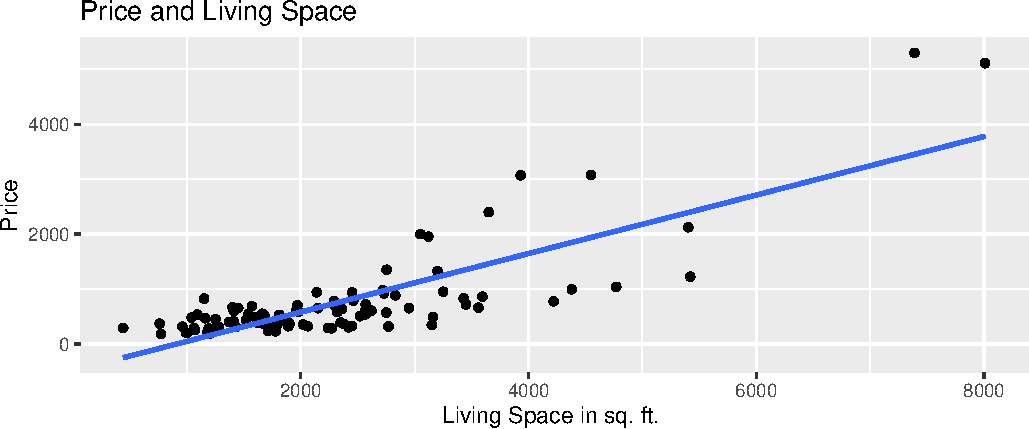
\includegraphics{Ch2_files/figure-pdf/unnamed-chunk-3-1.pdf}

The model equation is

\[
\widehat{\text{Price}} = b_0 + b_1\times\text{Sq.Ft.}
\]

Note, the symbol over the response variable (Price) is read as ``hat'',
and means ``predicted price''.

We fit the model in R, using the \texttt{lm} (linear model) command. The
output gives the estimates of \(b_0\) and \(b_1\).

\begin{Shaded}
\begin{Highlighting}[]
\NormalTok{M\_House\_sqft }\OtherTok{\textless{}{-}} \FunctionTok{lm}\NormalTok{(}\AttributeTok{data=}\NormalTok{Houses, price}\SpecialCharTok{\textasciitilde{}}\NormalTok{sqft\_living)}
\NormalTok{M\_House\_sqft}
\end{Highlighting}
\end{Shaded}

\begin{verbatim}

Call:
lm(formula = price ~ sqft_living, data = Houses)

Coefficients:
(Intercept)  sqft_living  
  -484.9575       0.5328  
\end{verbatim}

The estimates are \(b_0=-484.9575\) and \(b_1=0.5328\).

The model equation is

\[
\widehat{\text{Price}} = -484.9575 + 0.5328\times\text{Sq.Ft.}
\]

\textbf{Interpretations}

The intercept \(b_0\) represents the expected (or average) value of the
response variable, when the explanatory variable is equal to 0. This is
not always a meaningful interpretation in context.

The slope \(b_1\) represents the expected (or average) change in the
response variable for each one-unit increase in the explanatory
variable.

\begin{itemize}
\item
  On average, a house with 0 square feet is expected to cost -485
  thousand dollars. This is not a sensible interpretation, as there are
  no houses with 0 square feet.
\item
  For each additional square foot in living space, the price of the
  house is expected to increase by 0.5328 thousand dollars (or \$533).\\

  \begin{itemize}
  \tightlist
  \item
    Since a 1 square ft. increase is very small, it makes more sense to
    give the interpretation in terms of a 100-square foot increase. For
    each additional 100 square feet in living space, the price of the
    house is expected to increase by 53.28 thousand dollars.
  \end{itemize}
\end{itemize}

\textbf{Prediction}

We can predict the price of a house with a given number of square feet
by plugging the square feet into the model equation.

The predicted price of a house with 1,500 square feet is

\[
\widehat{\text{Price}} = -484.9575 + 0.5328\times 1500 = \$314{ \text{ thousand}}
\]

We can calculate this directly in R using the \texttt{predict} command.

\begin{Shaded}
\begin{Highlighting}[]
\FunctionTok{predict}\NormalTok{(M\_House\_sqft, }\AttributeTok{newdata=}\FunctionTok{data.frame}\NormalTok{(}\AttributeTok{sqft\_living=}\DecValTok{1500}\NormalTok{))}
\end{Highlighting}
\end{Shaded}

\begin{verbatim}
       1 
314.1803 
\end{verbatim}

We should only try to make predictions on houses within the range of the
observed data. Since the largest house in the dataset is 8,000 square
feet we should not try to predict the price of house with 10,000 square
feet.

\subsection{Categorical Explanatory
Variable}\label{categorical-explanatory-variable}

Next, we'll predict the price of a house based on whether or not it is
on the waterfront.

The boxplot shows the distribution of prices for waterfront and
nonwaterfront houses. The red dots indicate the mean.

\begin{Shaded}
\begin{Highlighting}[]
\FunctionTok{ggplot}\NormalTok{(}\AttributeTok{data=}\NormalTok{Houses, }\FunctionTok{aes}\NormalTok{(}\AttributeTok{x=}\NormalTok{waterfront, }\AttributeTok{y=}\NormalTok{price)) }\SpecialCharTok{+} \FunctionTok{geom\_boxplot}\NormalTok{() }\SpecialCharTok{+} 
  \FunctionTok{ggtitle}\NormalTok{(}\StringTok{"House Price by Waterfront Status"}\NormalTok{) }\SpecialCharTok{+} 
  \FunctionTok{xlab}\NormalTok{(}\StringTok{"Waterfront"}\NormalTok{) }\SpecialCharTok{+} \FunctionTok{ylab}\NormalTok{(}\StringTok{"Price"}\NormalTok{) }\SpecialCharTok{+} \FunctionTok{coord\_flip}\NormalTok{() }\SpecialCharTok{+} 
  \FunctionTok{stat\_summary}\NormalTok{(}\AttributeTok{fun.y=}\NormalTok{mean, }\AttributeTok{geom=}\StringTok{"point"}\NormalTok{, }\AttributeTok{shape=}\DecValTok{20}\NormalTok{, }\AttributeTok{color=}\StringTok{"red"}\NormalTok{, }\AttributeTok{fill=}\StringTok{"red"}\NormalTok{)}
\end{Highlighting}
\end{Shaded}

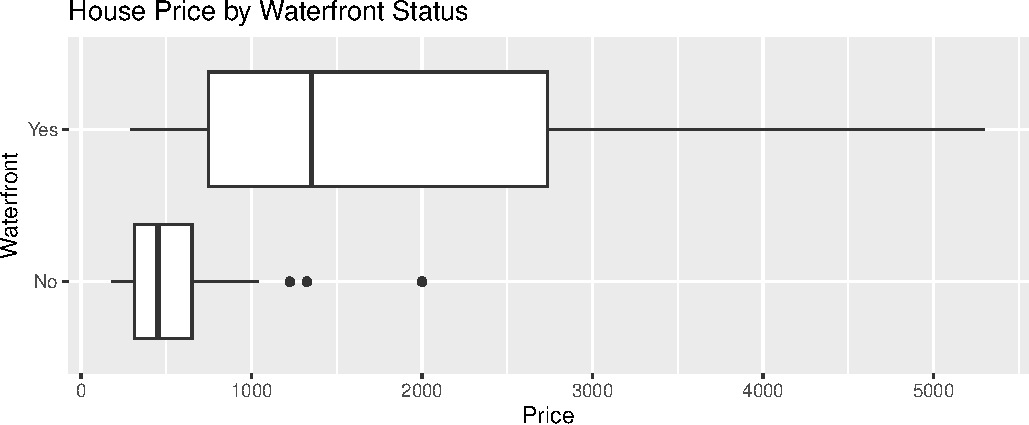
\includegraphics{Ch2_files/figure-pdf/unnamed-chunk-6-1.pdf}

The table displays the price summary by waterfront status.

\begin{Shaded}
\begin{Highlighting}[]
\NormalTok{Houses\_Grouped\_Summary }\OtherTok{\textless{}{-}}\NormalTok{ Houses }\SpecialCharTok{\%\textgreater{}\%} \FunctionTok{group\_by}\NormalTok{(waterfront) }\SpecialCharTok{\%\textgreater{}\%} 
                                      \FunctionTok{summarize}\NormalTok{(}\AttributeTok{Mean\_Price =} \FunctionTok{mean}\NormalTok{(price, }\AttributeTok{na.rm=}\ConstantTok{TRUE}\NormalTok{),}
                                                \AttributeTok{Median\_Price =} \FunctionTok{median}\NormalTok{(price, }\AttributeTok{na.rm=}\ConstantTok{TRUE}\NormalTok{), }
                                                \AttributeTok{StDev\_Price =} \FunctionTok{sd}\NormalTok{(price, }\AttributeTok{na.rm =} \ConstantTok{TRUE}\NormalTok{),}
                                                \AttributeTok{Number\_of\_Houses =} \FunctionTok{n}\NormalTok{()) }
\FunctionTok{kable}\NormalTok{(Houses\_Grouped\_Summary)}
\end{Highlighting}
\end{Shaded}

\begin{longtable}[]{@{}lrrrr@{}}
\toprule\noalign{}
waterfront & Mean\_Price & Median\_Price & StDev\_Price &
Number\_of\_Houses \\
\midrule\noalign{}
\endhead
\bottomrule\noalign{}
\endlastfoot
No & 523.7595 & 450 & 295.7991 & 85 \\
Yes & 1934.3800 & 1350 & 1610.7959 & 15 \\
\end{longtable}

The model equation is

\[
\widehat{\text{Price}} = b_0 + b_1\times\text{Waterfront}
\]

The waterfront variable takes on value of 1 if the house is on the
waterfront, and 0 otherwise.

\begin{Shaded}
\begin{Highlighting}[]
\NormalTok{M\_House\_wf }\OtherTok{\textless{}{-}} \FunctionTok{lm}\NormalTok{(}\AttributeTok{data=}\NormalTok{Houses, price}\SpecialCharTok{\textasciitilde{}}\NormalTok{waterfront)}
\NormalTok{M\_House\_wf}
\end{Highlighting}
\end{Shaded}

\begin{verbatim}

Call:
lm(formula = price ~ waterfront, data = Houses)

Coefficients:
  (Intercept)  waterfrontYes  
        523.8         1410.6  
\end{verbatim}

The estimates are \(b_0=523.8\) and \(b_1=1410.6\).

The model equation is

\[
\widehat{\text{Price}} = 523.8 + 1410.6\times \text{Waterfront}
\]

\textbf{Interpretations}

The intercept \(b_0\) represents the expected (or average) value of the
response variable in the ``baseline'' category (in this case
non-waterfront).

The coefficient \(b_1\) represents the expected (or average) difference
in response between the a category and the ``baseline'' category.

\begin{itemize}
\item
  On average, a house that is not on the waterfront is expected to cost
  523.8 thousand dollars.
\item
  On average a house that is on the waterfront is expected to cost
  1410.6 thousand (or 1.4 million) dollars more than a house that is not
  on the waterfront.
\end{itemize}

\textbf{Prediction}

We can predict the price of a house with a given number of square feet
by plugging in either 1 or 0 for the waterfront variable.

The predicted price of a house on the waterfront is:

\[
\widehat{\text{Price}} = 523.8 + 1410.6\times 1 = \$1934.6{ \text{ thousand (or 1.9 million)}}
\]

The predicted price of a house not on the waterfront is:

\[
\widehat{\text{Price}} = 523.8 + 1410.6\times 0 = \$523.8{ \text{ thousand}}
\]

Calculations in R:

\begin{Shaded}
\begin{Highlighting}[]
\FunctionTok{predict}\NormalTok{(M\_House\_wf, }\AttributeTok{newdata=}\FunctionTok{data.frame}\NormalTok{(}\AttributeTok{waterfront=}\StringTok{"Yes"}\NormalTok{))}
\end{Highlighting}
\end{Shaded}

\begin{verbatim}
      1 
1934.38 
\end{verbatim}

\begin{Shaded}
\begin{Highlighting}[]
\FunctionTok{predict}\NormalTok{(M\_House\_wf, }\AttributeTok{newdata=}\FunctionTok{data.frame}\NormalTok{(}\AttributeTok{waterfront=}\StringTok{"No"}\NormalTok{))}
\end{Highlighting}
\end{Shaded}

\begin{verbatim}
       1 
523.7595 
\end{verbatim}

Notice that the predicted prices for each category correspond to the
average price for that category.

\subsection{Multiple Explanatory
Variables}\label{multiple-explanatory-variables}

We've used square feet and waterfront status as explanatory variables
individually. We can also build a model that uses both of these
variables at the same time.

A model with two or more explanatory variables is called a
\textbf{multiple regression model}.

The model equation is

\[
\widehat{\text{Price}} = b_0 + b_1\times\text{Sq. Ft} + b_2\times\text{Waterfront}
\]

For a house not on the waterfront, \(b_2=0\), so the model equation is:

\[
\widehat{\text{Price}} = b_0  + b_1\text{Sq. Ft} 
\]

For a house on the waterfront, \(b_2=1\), so the model equation is:

\[
\widehat{\text{Price}} = (b_0 + b_2) + b_1\times\text{Sq. Ft} 
\]

Notice that the slope is the same, regardless of whether the house is on
the waterfront (\(b_1\)). The intercept, however, is different (\(b_0\)
for houses not on the waterfront, and \(b_0 + b_2\) for houses on the
waterfront). Thus, the model assumes that price increases at the same
rate, with respect to square feet, regardless of whether or not it is on
the waterfront, but allows the predicted price for a waterfront house to
differ from a non-waterfront house of the same size.

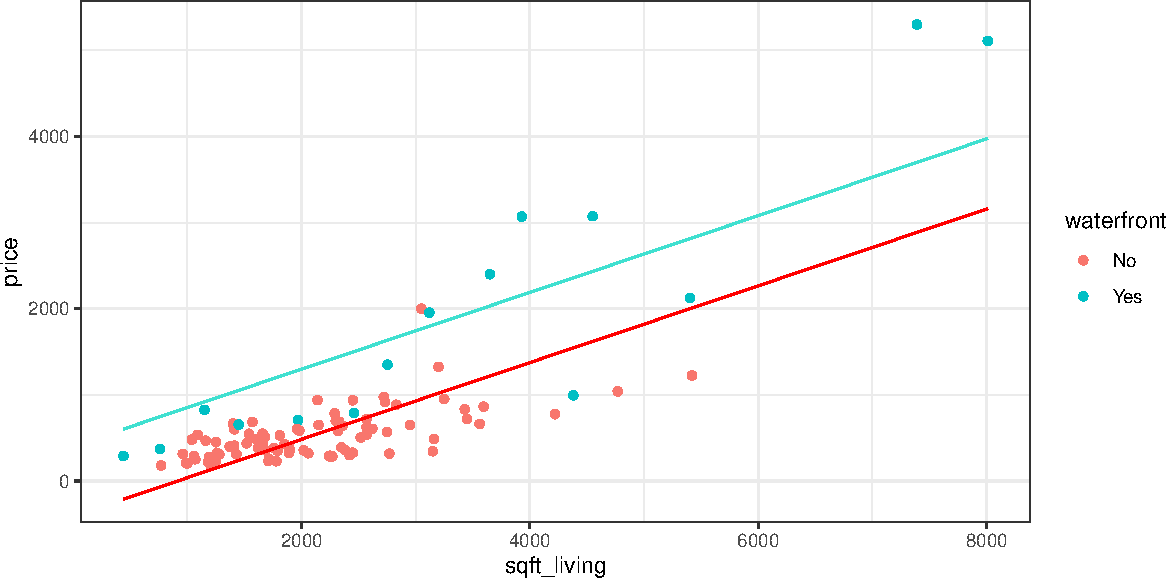
\includegraphics{Ch2_files/figure-pdf/unnamed-chunk-12-1.pdf}

We fit the model in R.

\begin{Shaded}
\begin{Highlighting}[]
\NormalTok{M\_wf\_sqft }\OtherTok{\textless{}{-}} \FunctionTok{lm}\NormalTok{(}\AttributeTok{data=}\NormalTok{Houses, price}\SpecialCharTok{\textasciitilde{}}\NormalTok{sqft\_living}\SpecialCharTok{+}\NormalTok{waterfront)}
\NormalTok{M\_wf\_sqft}
\end{Highlighting}
\end{Shaded}

\begin{verbatim}

Call:
lm(formula = price ~ sqft_living + waterfront, data = Houses)

Coefficients:
  (Intercept)    sqft_living  waterfrontYes  
    -407.6549         0.4457       814.3613  
\end{verbatim}

The model equation is

\[
\widehat{\text{Price}} = -407.7 + 0.4457\times\text{Sq. Ft} + 814.36\times\text{Waterfront}
\]

\textbf{Interpretations}

The intercept \(b_0\) represents the expected (or average) value of the
response variable, when all quantitative explanatory variables are equal
to 0, and all categorical variables are in the ``baseline'' category.
This interpretion is not always sensible.

We interpret coefficients \(b_j\) for categorical or quantitative
variables, the same way we would in a regression model with only one
variable, but we need to state that all other explanatory variables are
being held constant.

\begin{itemize}
\item
  On average, a house that is not on the waterfront with 0 square feet
  is expected to cost -407.7 thousand dollars. This is not a sensible
  interpretation, since there are no houses with 0 square feet.\\
\item
  For each 1-square foot increase in size, the price of a house is
  expected to increase by 0.4457 thousand (or 446 hundred) dollars,
  assuming waterfront status is the same. Equivalently, for each
  100-square foot increase in size, the price of a house is expected to
  increase by 44.57 thousand dollars, assuming waterfront status is the
  same.
\item
  On average, a house on the waterfront is expected to cost 814 thousand
  dollars more than a house that is not on the waterfront, assuming
  square footage is the same.
\end{itemize}

\textbf{Prediction}

The predicted price of a 1,500 square foot house on the waterfront is:

\[
\widehat{\text{Price}} = -407.7 + 0.4457\times1500 + 814.36\times1 = \$1075{ \text{ thousand (or 1.075 million)}}
\]

The predicted price of a 1,500 square foot not on the waterfront is:

\[
\widehat{\text{Price}} = -407.7 + 0.4457\times1500 = \$260.9{ \text{ thousand}}
\]

Calculations in R:

\begin{Shaded}
\begin{Highlighting}[]
\FunctionTok{predict}\NormalTok{(M\_wf\_sqft, }\AttributeTok{newdata=}\FunctionTok{data.frame}\NormalTok{(}\AttributeTok{waterfront=}\StringTok{"Yes"}\NormalTok{, }\AttributeTok{sqft\_living=}\DecValTok{1500}\NormalTok{))}
\end{Highlighting}
\end{Shaded}

\begin{verbatim}
       1 
1075.227 
\end{verbatim}

\begin{Shaded}
\begin{Highlighting}[]
\FunctionTok{predict}\NormalTok{(M\_wf\_sqft, }\AttributeTok{newdata=}\FunctionTok{data.frame}\NormalTok{(}\AttributeTok{waterfront=}\StringTok{"No"}\NormalTok{, }\AttributeTok{sqft\_living=}\DecValTok{1500}\NormalTok{))}
\end{Highlighting}
\end{Shaded}

\begin{verbatim}
       1 
260.8657 
\end{verbatim}

\subsection{No Explanatory Variable}\label{no-explanatory-variable}

Finally, we'll consider a model that makes use of no explanatory
variables at all. Although this might seem silly, its relevance will be
seen in the next section.

The histogram shows the distribution of prices, without any information
about explanatory variables. The mean price is indicated in red.

\begin{Shaded}
\begin{Highlighting}[]
\FunctionTok{ggplot}\NormalTok{(}\AttributeTok{data=}\NormalTok{Houses, }\FunctionTok{aes}\NormalTok{(}\AttributeTok{x=}\NormalTok{price)) }\SpecialCharTok{+} 
  \FunctionTok{geom\_histogram}\NormalTok{(}\AttributeTok{fill=}\StringTok{"lightblue"}\NormalTok{, }\AttributeTok{color=}\StringTok{"white"}\NormalTok{) }\SpecialCharTok{+} 
  \FunctionTok{ggtitle}\NormalTok{(}\StringTok{"Distribution of House Prices"}\NormalTok{) }\SpecialCharTok{+} \FunctionTok{xlab}\NormalTok{(}\StringTok{"Price"}\NormalTok{) }\SpecialCharTok{+} \FunctionTok{ylab}\NormalTok{(}\StringTok{"Frequency"}\NormalTok{) }\SpecialCharTok{+} 
  \FunctionTok{geom\_point}\NormalTok{(}\FunctionTok{aes}\NormalTok{(}\AttributeTok{x=}\FunctionTok{mean}\NormalTok{(Houses}\SpecialCharTok{$}\NormalTok{price), }\AttributeTok{y=}\DecValTok{0}\NormalTok{), }\AttributeTok{color=}\StringTok{"red"}\NormalTok{, }\AttributeTok{shape=}\DecValTok{24}\NormalTok{, }\AttributeTok{fill=}\StringTok{"red"}\NormalTok{)}
\end{Highlighting}
\end{Shaded}

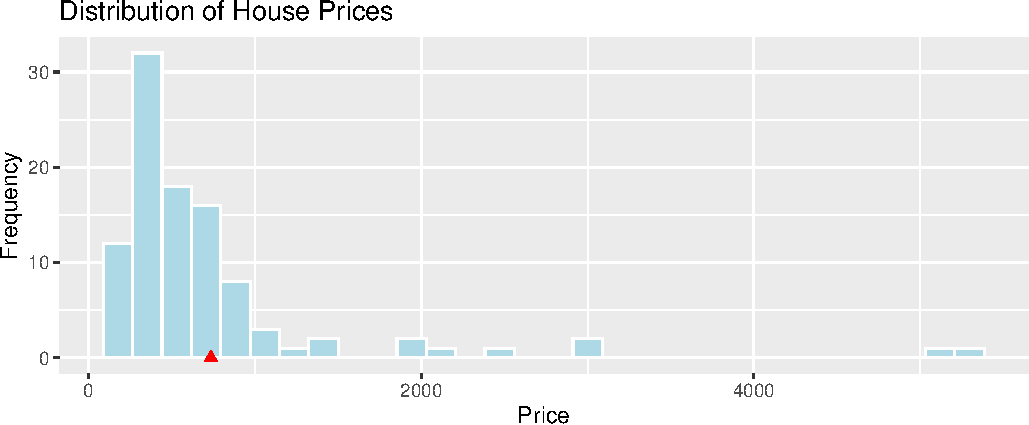
\includegraphics{Ch2_files/figure-pdf/unnamed-chunk-16-1.pdf}

The mean, median, and standard deviation in prices is shown below.

\begin{Shaded}
\begin{Highlighting}[]
\FunctionTok{library}\NormalTok{(knitr)}
\FunctionTok{kable}\NormalTok{(Houses\_Summary)}
\end{Highlighting}
\end{Shaded}

\begin{longtable}[]{@{}rrrr@{}}
\toprule\noalign{}
Mean\_Price & Median\_Price & StDev\_Price & Number\_of\_Houses \\
\midrule\noalign{}
\endhead
\bottomrule\noalign{}
\endlastfoot
735.3525 & 507.5 & 835.1231 & 100 \\
\end{longtable}

Suppose we know that a house sold in King County during this time, and
want to predict the price, without knowing anything else about the
house.

The best we can do is to use the mean price for our prediction. (We'll
define what we mean by ``best'' later in the chapter.)

The model equation is

\[
\widehat{\text{Price}} = b_0
\]

We fit a statistical model in R using the \texttt{lm} command.

\begin{Shaded}
\begin{Highlighting}[]
\CommentTok{\# syntax for lm command}
\CommentTok{\# lm(data=DatasetName, ResponseVariable\textasciitilde{}ExplanatoryVariable(s))}

\NormalTok{M0\_House }\OtherTok{\textless{}{-}} \FunctionTok{lm}\NormalTok{(}\AttributeTok{data=}\NormalTok{Houses, price }\SpecialCharTok{\textasciitilde{}} \DecValTok{1}\NormalTok{) }\CommentTok{\# when there are no explanatory variables, use \textasciitilde{}1}
\NormalTok{M0\_House}
\end{Highlighting}
\end{Shaded}

\begin{verbatim}

Call:
lm(formula = price ~ 1, data = Houses)

Coefficients:
(Intercept)  
      735.4  
\end{verbatim}

The model equation is

\[
\widehat{\text{Price}} = 735.4
\]

\textbf{Interpretation}

The expected price of a house in King County is 735.4 thousand dollars.

\textbf{Predictions}

Without knowing anything about any explanatory variables, we would
predict the price of any house sold in King County, WA to cost 735.4
thousand dollars.

\section{Variability Explained by a
Model}\label{variability-explained-by-a-model}

We've seen four different models for predicting house price. It would be
nice to have a way to assess how well the models are predicting prices,
and determine which model appears to be the best.

Of course we won't know the price of the house we are trying to predict,
so we can't be sure how close or far our prediction is. We do, however,
know the prices of the original 100 houses in our dataset. We can assess
the models by measuring how far the actual prices of the 100 houses
differ from the predicted (mean) price, and by calculating the
proportion of total variation in sale price explained by each model.

\subsection{Total Variability}\label{total-variability}

Let's start with our most basic model, which uses no explanatory
variables and predicts the price of each simply using the average of all
houses in the dataset.

We measure the total variability in the response variable by calculating
the square difference between each individual response value and the
overall average. This quantity is called the total sum of squares (SST).

\[
\text{SST} = \displaystyle\sum_{i=1}^n (y_i - \bar{y})^2
\]

The plot below shows a horizontal line at the mean sale price (785
thousand). The points represent prices of individual houses, and the red
lines represent the differences between the price of each house and the
overall average.

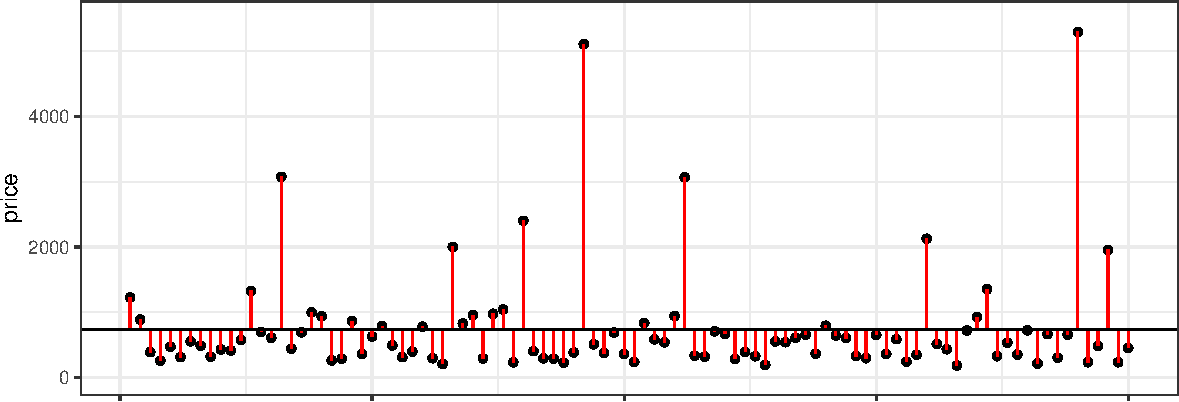
\includegraphics{Ch2_files/figure-pdf/unnamed-chunk-19-1.pdf}

The first three houses in the dataset are shown below.

\begin{Shaded}
\begin{Highlighting}[]
\NormalTok{First3Houses }\OtherTok{\textless{}{-}}\NormalTok{ Houses }\SpecialCharTok{\%\textgreater{}\%} \FunctionTok{select}\NormalTok{(Id, price, waterfront, sqft\_living) }\SpecialCharTok{\%\textgreater{}\%} \FunctionTok{head}\NormalTok{(}\DecValTok{3}\NormalTok{)}
\FunctionTok{kable}\NormalTok{(First3Houses)}
\end{Highlighting}
\end{Shaded}

\begin{longtable}[]{@{}rrlr@{}}
\toprule\noalign{}
Id & price & waterfront & sqft\_living \\
\midrule\noalign{}
\endhead
\bottomrule\noalign{}
\endlastfoot
1 & 1225 & No & 5420 \\
2 & 885 & No & 2830 \\
3 & 385 & No & 1620 \\
\end{longtable}

\[
\begin{aligned}
\text{SST} & = \displaystyle\sum_{i=1}^{100} (y_i - \bar{y})^2 \\
& = (1225-785)^2 + (885-785)^2 + (385-785)^2 + \ldots 
\end{aligned}
\]

We could calculate SST by hand for small datasets. For larger datasets,
we'll use R to perform the calculation.

\begin{Shaded}
\begin{Highlighting}[]
\NormalTok{meanprice }\OtherTok{\textless{}{-}} \FunctionTok{mean}\NormalTok{(Houses}\SpecialCharTok{$}\NormalTok{price)  }\CommentTok{\#calculate mean price}
\NormalTok{SST }\OtherTok{\textless{}{-}} \FunctionTok{sum}\NormalTok{((Houses}\SpecialCharTok{$}\NormalTok{price }\SpecialCharTok{{-}}\NormalTok{ meanprice)}\SpecialCharTok{\^{}}\DecValTok{2}\NormalTok{)  }\DocumentationTok{\#\# calculate SST}
\NormalTok{SST}
\end{Highlighting}
\end{Shaded}

\begin{verbatim}
[1] 69045634
\end{verbatim}

By itself, the size of SST does not have much meaning. We cannot say
whether a SST value like the one we see here is large or small, since it
depends on the size and scale of the variable being measured. An SST
value that is very large in one context might be very small in another.

SST does, however, give us a baseline measure of the total variability
in the response variable. We'll assess the performance of a model with a
given explanatory variable by measuring how much of this variability the
model accounts for.

\subsection{Residuals}\label{residuals}

Now let's consider our model that uses the size of the house in square
feet as the explanatory variable. The figure on the left shows
difference between actual and predicted prices, using this linear model.
We compare the size of the differences to those resulting from the basic
model that does not use any explanatory variables, and predicts each
price using the overall average (shown on the right).

\begin{Shaded}
\begin{Highlighting}[]
\NormalTok{Residplot\_sqft }\OtherTok{\textless{}{-}} \FunctionTok{ggplot}\NormalTok{(}\AttributeTok{data=}\NormalTok{Houses, }\FunctionTok{aes}\NormalTok{(}\AttributeTok{x =}\NormalTok{ sqft\_living, }\AttributeTok{y =}\NormalTok{ price)) }\SpecialCharTok{+}  \FunctionTok{geom\_point}\NormalTok{() }\SpecialCharTok{+}
                \FunctionTok{geom\_segment}\NormalTok{(}\FunctionTok{aes}\NormalTok{(}\AttributeTok{xend =}\NormalTok{ sqft\_living, }\AttributeTok{yend =}\NormalTok{ M\_House\_sqft}\SpecialCharTok{$}\NormalTok{fitted.values), }\AttributeTok{color=}\StringTok{"red"}\NormalTok{) }\SpecialCharTok{+}
                \FunctionTok{geom\_point}\NormalTok{(}\FunctionTok{aes}\NormalTok{(}\AttributeTok{y =}\NormalTok{ M\_House\_sqft}\SpecialCharTok{$}\NormalTok{fitted.values), }\AttributeTok{shape =} \DecValTok{1}\NormalTok{) }\SpecialCharTok{+}
                \FunctionTok{stat\_smooth}\NormalTok{(}\AttributeTok{method=}\StringTok{"lm"}\NormalTok{, }\AttributeTok{se=}\ConstantTok{FALSE}\NormalTok{) }\SpecialCharTok{+} \FunctionTok{ylim}\NormalTok{(}\FunctionTok{c}\NormalTok{(}\DecValTok{0}\NormalTok{,}\DecValTok{5500}\NormalTok{)) }\SpecialCharTok{+}
                \FunctionTok{theme\_bw}\NormalTok{() }
\end{Highlighting}
\end{Shaded}

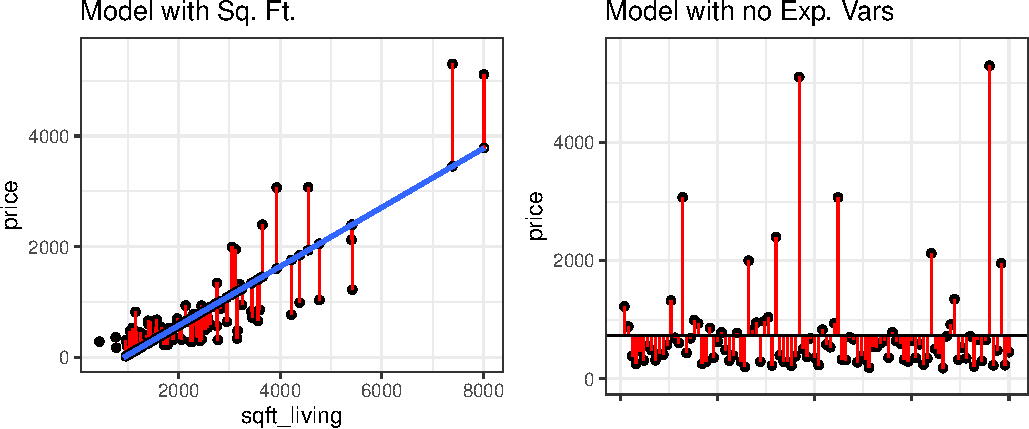
\includegraphics{Ch2_files/figure-pdf/unnamed-chunk-23-1.pdf}

Notice that the red lines are shorter in the figure on the left,
indicating the predictions are closer to the actual values.

The difference between the actual and predicted values is called the
\textbf{residual}. The residual for the \(ith\) case is

\[
r_i = (y_i-\hat{y}_i)
\]

We'll calculate the residuals for the first three houses in the dataset,
shown below.

\begin{Shaded}
\begin{Highlighting}[]
\FunctionTok{kable}\NormalTok{(First3Houses)}
\end{Highlighting}
\end{Shaded}

\begin{longtable}[]{@{}rrlr@{}}
\toprule\noalign{}
Id & price & waterfront & sqft\_living \\
\midrule\noalign{}
\endhead
\bottomrule\noalign{}
\endlastfoot
1 & 1225 & No & 5420 \\
2 & 885 & No & 2830 \\
3 & 385 & No & 1620 \\
\end{longtable}

The model equation is

\[
\widehat{\text{Price}} = -484.9575 + 0.5328\times \text{Sq. Ft} 
\]

The predicted prices for these three houses are:

\[
\widehat{\text{Price}_1} = -484.9575 + 0.5328\times 5420 = 2402.6 \text{ thousand dollars}
\]

\[
\widehat{\text{Price}_2} = -484.9575 + 0.5328\times 2830 = 1022.7 \text{ thousand dollars}
\]

\[
\widehat{\text{Price}_3} = -484.9575 + 0.5328\times 1620 = 378.1 \text{ thousand dollars}
\]

To calculate the residuals, we subtract the predicted price from the
actual price.

\[r_1 = y_1-\hat{y}_1 = 1225 - 2402.6 = -1177.6 \text{ thousand dollars}\]

\[r_2 = y_2-\hat{y}_2 = 885 - 1022.7 = -137.7 \text{ thousand dollars}\]

\[r_2 = y_2-\hat{y}_2 = 385 - 378.1 = 6.9 \text{ thousand dollars}\]

The fact that the first two residuals are negative indicates that these
houses sold for less than the model predicts.

The predicted values and residuals from a model can be calculated
automatically in R. The predicted values and residuals for the first 5
houses are shown below.

\begin{Shaded}
\begin{Highlighting}[]
\NormalTok{Predicted }\OtherTok{\textless{}{-}} \FunctionTok{predict}\NormalTok{(M\_House\_sqft)}
\FunctionTok{head}\NormalTok{(Predicted, }\DecValTok{3}\NormalTok{)}
\end{Highlighting}
\end{Shaded}

\begin{verbatim}
        1         2         3 
2402.5937 1022.7491  378.1113 
\end{verbatim}

\begin{Shaded}
\begin{Highlighting}[]
\NormalTok{Residual }\OtherTok{\textless{}{-}}\NormalTok{ M\_House\_sqft}\SpecialCharTok{$}\NormalTok{residuals}
\FunctionTok{head}\NormalTok{(Residual, }\DecValTok{3}\NormalTok{)}
\end{Highlighting}
\end{Shaded}

\begin{verbatim}
           1            2            3 
-1177.593665  -137.749128     6.888668 
\end{verbatim}

\subsection{Variability Explained by Sq. Ft.
Model}\label{variability-explained-by-sq.-ft.-model}

The \textbf{sum of squared residuals (SSR)} measures the amount of
unexplained variability in the response variable after accounting for
all explanatory variables in the model.

\[
\text{SSR} = \displaystyle\sum_{i=1}^{n}(y_i-\hat{y}_i)^2.  
\]

Note that SSR is similar to SST, except we subtract the model's
predicted values, rather than the overall average. In the special case
of a model with no explanatory variables, the predicted values are equal
to the overall average, so SSR is equal to SST.

We calculate SSR for the model using square feet as the explanatory
variable.

\[
\begin{aligned}
\text{SSR} & = \displaystyle\sum_{i=1}^{n}(y_i-\hat{y}_i)^2.  \\
 & = (1225 - 2402.6)^2 + (885 - 1022.7)^2 + (385 - 378.1)^2 + \ldots
\end{aligned}
\]

We can calculate the model's SSR directly in R.

\begin{Shaded}
\begin{Highlighting}[]
\NormalTok{SSR\_sqft }\OtherTok{\textless{}{-}} \FunctionTok{sum}\NormalTok{(M\_House\_sqft}\SpecialCharTok{$}\NormalTok{residuals}\SpecialCharTok{\^{}}\DecValTok{2}\NormalTok{)}
\NormalTok{SSR\_sqft}
\end{Highlighting}
\end{Shaded}

\begin{verbatim}
[1] 23767280
\end{verbatim}

SSR represents the amount of total variability in saleprice remaining
after accounting for the house's size in square feet.

The SSR=23,767,290 value is about one third of the SST value of
69,045,634. This means that about 2/3 of the total variability in sale
price is explained by the model that accounts for sale price.

The difference (SST-SSR) represents the variability in the response
variable that is explained by the model. This quantity is called the
\textbf{model sum of squares (SSM)}.

\[ \text{SSM} = \text{SST} - \text{SSR} \]

It can be shown that
\(\text{SSM}=\displaystyle\sum_{i=1}^n(\hat{y}_i-\bar{y})^2\).

The proportion of total variability in the response variable explained
by the model is called the \textbf{coefficient of determination},
denoted \(R^2\). We calculate this by dividing SSM by SST.

\[
R^2=\frac{SSM}{SST}= \frac{SST-SSR}{SST}
\]

\textbf{Example:} For the model with square feet as the explanatory
variable,

\[
SSM = SST-SSR = 69,045,634 - 23,767,290 =45,278,344.
\]

\[
R^2 = \frac{45,278,344}{69,045,634}=0.6557.
\]

Approximately 65.6\% of the total variability in sale price is explained
by the model using square feet as the explanatory variable.

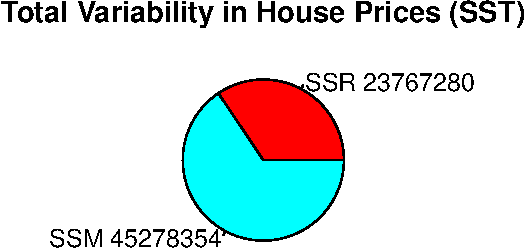
\includegraphics{Ch2_files/figure-pdf/unnamed-chunk-28-1.pdf}

We calculate \(R^2\) directly in R.

\begin{Shaded}
\begin{Highlighting}[]
\FunctionTok{summary}\NormalTok{(M\_House\_sqft)}\SpecialCharTok{$}\NormalTok{r.squared}
\end{Highlighting}
\end{Shaded}

\begin{verbatim}
[1] 0.6557743
\end{verbatim}

\subsection{Linear Correlation
Coefficient}\label{linear-correlation-coefficient}

For models with a single quantiative explanatory varible, the
coefficient of determination is equal to the square of the correlation
coefficient \(r\), discussed in Chapter 1.

\begin{Shaded}
\begin{Highlighting}[]
\FunctionTok{ggplot}\NormalTok{(}\AttributeTok{data=}\NormalTok{Houses, }\FunctionTok{aes}\NormalTok{(}\AttributeTok{x=}\NormalTok{sqft\_living, }\AttributeTok{y=}\NormalTok{price)) }\SpecialCharTok{+} \FunctionTok{geom\_point}\NormalTok{() }\SpecialCharTok{+} 
  \FunctionTok{stat\_smooth}\NormalTok{(}\AttributeTok{method=}\StringTok{"lm"}\NormalTok{, }\AttributeTok{se=}\ConstantTok{FALSE}\NormalTok{)}
\end{Highlighting}
\end{Shaded}

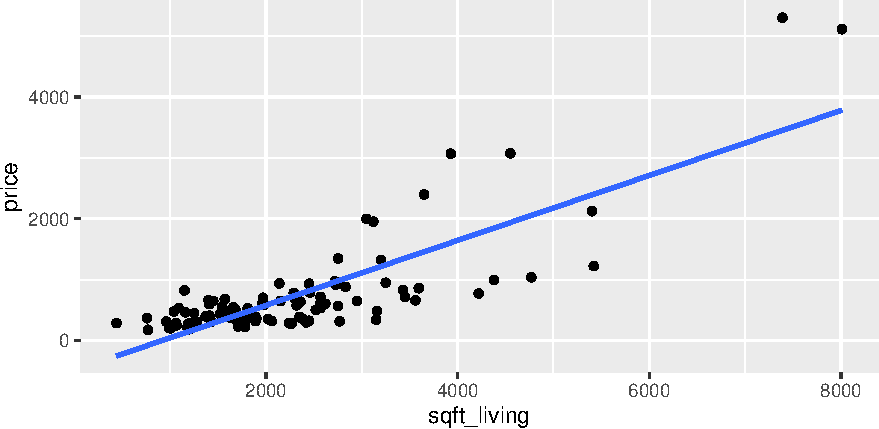
\includegraphics{Ch2_files/figure-pdf/unnamed-chunk-30-1.pdf}

\begin{itemize}
\item
  For linear models with a single quantitative variable, the
  \textbf{linear correlation coefficient} \(r=\sqrt{R^2}\), or
  \(r=-\sqrt{R^2}\) (with sign matching the sign on the slope of the
  line), provides information about the strength and direction of the
  linear relationship between the variables.
\item
  \(-1 \leq r \leq 1\), and \(r\) close to \(\pm1\) provides evidence of
  strong linear relationship, while \(r\) close to 0 suggests linear
  relationship is weak.
\end{itemize}

\begin{Shaded}
\begin{Highlighting}[]
\FunctionTok{cor}\NormalTok{(Houses}\SpecialCharTok{$}\NormalTok{price,Houses}\SpecialCharTok{$}\NormalTok{sqft\_living)}
\end{Highlighting}
\end{Shaded}

\begin{verbatim}
[1] 0.8097989
\end{verbatim}

\begin{itemize}
\tightlist
\item
  \(r\) is only relevant for models with a single quantitative
  explanatory variable and a quantitative response variable, while
  \(R^2\) is relevant for any linear model with a quantitative response
  variable.
\end{itemize}

\subsection{Variability Explained by Waterfront
Model}\label{variability-explained-by-waterfront-model}

We can similarly calculate the proportion of variability explained by
the model using waterfront as an explanatory variable.

Recall that in this model, the predicted price of a house with a
waterfront is given by the average price of all waterfront houses, and
the predicted price of a non-waterfront house is given by the average
price of all non-waterfront houses.

We can calculate residuals using these predicted values, and compare
them to the residuals resulting from a model with no explanatory
variables, which uses the overall average price for all predictions.

The left two figures show the residuals resulting from a model that
accounts for waterfront status. The figure on the right shows the
residuals resulting from the model with no explanatory variables.

\begin{Shaded}
\begin{Highlighting}[]
\FunctionTok{grid.arrange}\NormalTok{(}\FunctionTok{arrangeGrob}\NormalTok{(M1aResid,M1bResid, Residplot\_M0 }\SpecialCharTok{+} \FunctionTok{ggtitle}\NormalTok{(}\StringTok{"Model with no Exp. Vars"}\NormalTok{), }\AttributeTok{ncol=}\DecValTok{3}\NormalTok{, }\AttributeTok{nrow=}\DecValTok{1}\NormalTok{, }\AttributeTok{widths=}\FunctionTok{c}\NormalTok{(}\DecValTok{3}\NormalTok{, }\DecValTok{2}\NormalTok{,}\DecValTok{5}\NormalTok{))) }
\end{Highlighting}
\end{Shaded}

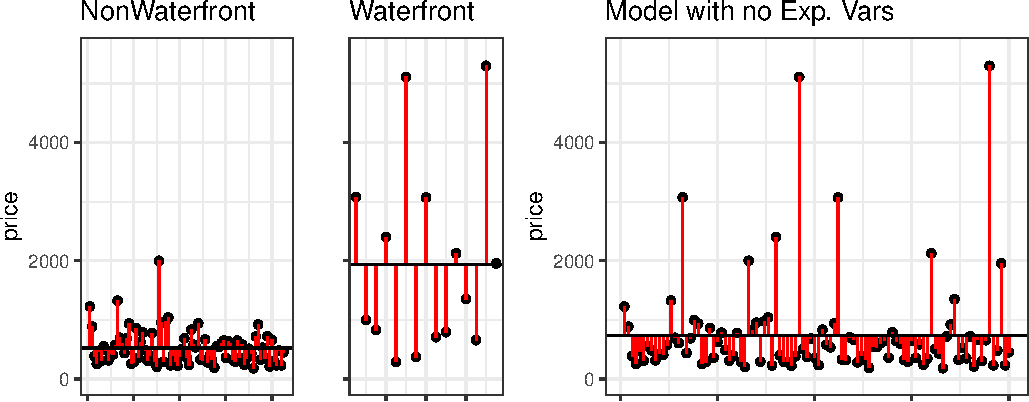
\includegraphics{Ch2_files/figure-pdf/unnamed-chunk-33-1.pdf}

Notice that after accounting for waterfront status, the differences
between observed and predicted values are bigger than they were in the
model that accounted for square feet, though not as big as for the model
that doesn't use any explanatory variables.

We use R to calculate SSR for the waterfront model.

\begin{Shaded}
\begin{Highlighting}[]
\NormalTok{SSR\_wf }\OtherTok{\textless{}{-}} \FunctionTok{sum}\NormalTok{(M\_House\_wf}\SpecialCharTok{$}\NormalTok{residuals}\SpecialCharTok{\^{}}\DecValTok{2}\NormalTok{)}
\NormalTok{SSR\_wf}
\end{Highlighting}
\end{Shaded}

\begin{verbatim}
[1] 43675043
\end{verbatim}

\[
SSM = SST-SSR = 69,045,634 - 43,675,043 =25,370,591.
\]

\[
R^2 = \frac{25,370,591}{69,045,634}=0.3674.
\]

Approximately 36.7\% of the total variability in sale price is explained
by the model using waterfront status as the explanatory variable.

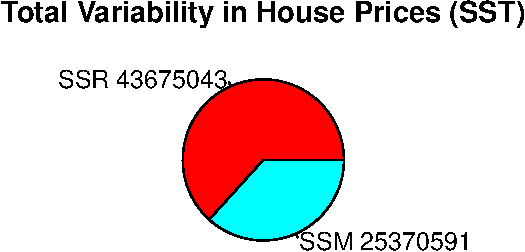
\includegraphics{Ch2_files/figure-pdf/unnamed-chunk-35-1.pdf}

We calculate \(R^2\) directly in R.

\begin{Shaded}
\begin{Highlighting}[]
\FunctionTok{summary}\NormalTok{(M\_House\_wf)}\SpecialCharTok{$}\NormalTok{r.squared}
\end{Highlighting}
\end{Shaded}

\begin{verbatim}
[1] 0.3674467
\end{verbatim}

\subsection{Variability Explained by Multiple Regression
Model}\label{variability-explained-by-multiple-regression-model}

We've seen at the model using square feet accounts for about 2/3 of the
total variability in house prices, while the model using waterfront
status accounts for about 1/3 of the total variability. Let's see if we
can do better by using both variables together.

The left figure shows the residuals resulting from a model that accounts
for both waterfront status and square feet. The figure on the right
shows the residuals resulting from the model with no explanatory
variables.

\begin{Shaded}
\begin{Highlighting}[]
\FunctionTok{grid.arrange}\NormalTok{(Residplot\_MR }\SpecialCharTok{+} \FunctionTok{ggtitle}\NormalTok{(}\StringTok{"Multiple Regression Model"}\NormalTok{) , Residplot\_M0 }\SpecialCharTok{+} \FunctionTok{ggtitle}\NormalTok{(}\StringTok{"Model with no Exp. Vars"}\NormalTok{), }\AttributeTok{ncol=}\DecValTok{2}\NormalTok{)}
\end{Highlighting}
\end{Shaded}

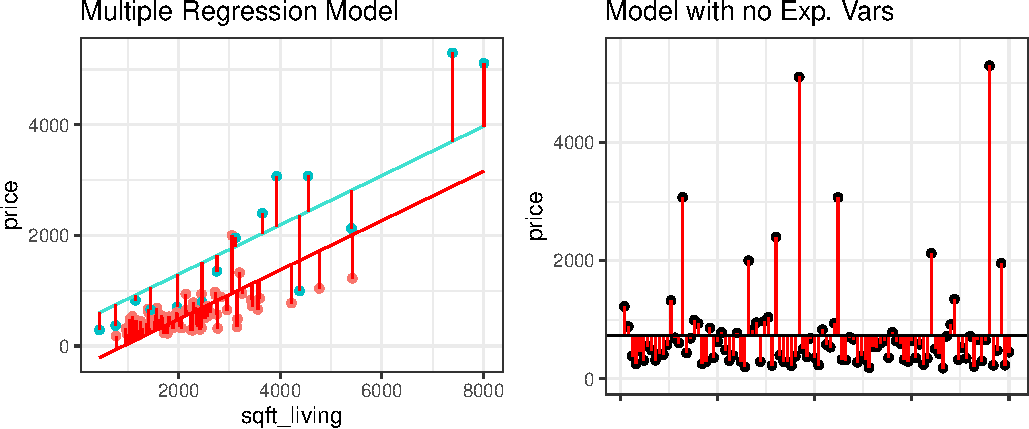
\includegraphics{Ch2_files/figure-pdf/unnamed-chunk-38-1.pdf}

We use R to calculate SSR for the waterfront model.

\begin{Shaded}
\begin{Highlighting}[]
\NormalTok{SSR\_wf\_sqft }\OtherTok{\textless{}{-}} \FunctionTok{sum}\NormalTok{(M\_wf\_sqft}\SpecialCharTok{$}\NormalTok{residuals}\SpecialCharTok{\^{}}\DecValTok{2}\NormalTok{)}
\NormalTok{SSR\_wf\_sqft}
\end{Highlighting}
\end{Shaded}

\begin{verbatim}
[1] 16521296
\end{verbatim}

\[
SSM = SST-SSR = 69,045,634 - 16,521,296 =52,524,338.
\]

\[
R^2 = \frac{52,524,338}{69,045,634}=0.761.
\]

Approximately 76.1\% of the total variability in sale price is explained
by the model using square feet and waterfront status as the explanatory
variables.

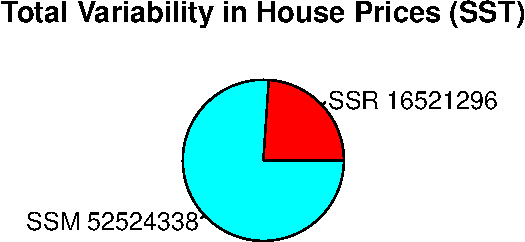
\includegraphics{Ch2_files/figure-pdf/unnamed-chunk-40-1.pdf}

We calculate \(R^2\) directly in R.

\begin{Shaded}
\begin{Highlighting}[]
\FunctionTok{summary}\NormalTok{(M\_wf\_sqft)}\SpecialCharTok{$}\NormalTok{r.squared}
\end{Highlighting}
\end{Shaded}

\begin{verbatim}
[1] 0.7607192
\end{verbatim}

Including both square feet and waterfront status allows us to explain
more variability in sale price than models that include one but not both
of these variables.

\subsection{\texorpdfstring{Summary: SST, SSR, SSM,
\(R^2\)}{Summary: SST, SSR, SSM, R\^{}2}}\label{summary-sst-ssr-ssm-r2}

\begin{itemize}
\tightlist
\item
  the total variability in the response variable is the sum of the
  squared differences between the observed values and the overall
  average.
\end{itemize}

\[\text{Total Variability in Response Var.}= \text{SST} =\displaystyle\sum_{i=1}^n(y_i-\bar{y})^2\]

\begin{itemize}
\tightlist
\item
  the variability remaining unexplained even after accounting for
  explanatory variable(s) in a model is given by the sum of squared
  residuals. We abbreviate this SSR, for sum of squared residuals.
\end{itemize}

\[
\text{SSR} = \text{Variability Remaining}=\displaystyle\sum_{i=1}^n(y_i-\hat{y}_i)^2
\]

\begin{itemize}
\tightlist
\item
  the variability explained by the model, abbreviated SSM, is given by
\end{itemize}

\[ \text{SSM} = \text{SST} - \text{SSR} \]

\begin{itemize}
\tightlist
\item
  The coefficient of determination (abbreviated \(R^2\)) is defined as
\end{itemize}

\[R^2=\frac{\text{Variability Explained by Model}}{\text{Total Variability}}=\frac{\text{SSM}}{\text{SST}} =\frac{\displaystyle\sum_{i=1}^n(\hat{y}_i-\bar{y})^2}{\displaystyle\sum_{i=1}^n(y_i-\bar{y})^2}\]

Note that some texts use different abbreviations than the ones used
here. When working with resources outside this class, be sure to
carefully check the notation being used.

For the model with a single quantitative explanatory variable.

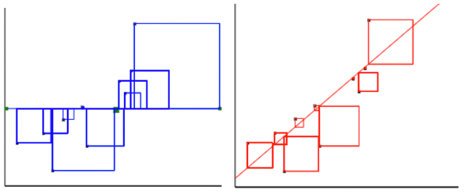
\includegraphics[width=1\textwidth,height=\textheight]{Rsq.png}

Model with a single categorical explanatory variable with 3 categories:

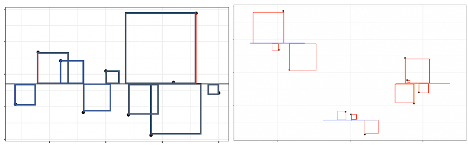
\includegraphics[width=1\textwidth,height=\textheight]{Rsq2.png}

\begin{itemize}
\item
  Blue Area = Total Variability (SST)
\item
  Red Area = Variability Remaining Unexplained by Model (SSR)
\item
  Blue Area - Red Area = Variability Explained by Model (SSM)
\item
  \(R^2 = \frac{\text{Area of Blue Squares} - \text{Area of Red Squares}}{\text{Area of Blue Squares}} = \frac{\text{SST}-\text{SSR}}{\text{SST}}= \frac{\text{SSM}}{\text{SST}}\)
\end{itemize}

\subsection{Model Comparison Summary}\label{model-comparison-summary}

\begin{longtable}[]{@{}
  >{\raggedright\arraybackslash}p{(\columnwidth - 8\tabcolsep) * \real{0.0660}}
  >{\raggedright\arraybackslash}p{(\columnwidth - 8\tabcolsep) * \real{0.2264}}
  >{\raggedright\arraybackslash}p{(\columnwidth - 8\tabcolsep) * \real{0.2358}}
  >{\raggedright\arraybackslash}p{(\columnwidth - 8\tabcolsep) * \real{0.2170}}
  >{\raggedright\arraybackslash}p{(\columnwidth - 8\tabcolsep) * \real{0.2547}}@{}}
\toprule\noalign{}
\begin{minipage}[b]{\linewidth}\raggedright
Model
\end{minipage} & \begin{minipage}[b]{\linewidth}\raggedright
Variables
\end{minipage} & \begin{minipage}[b]{\linewidth}\raggedright
Unexplained Variability
\end{minipage} & \begin{minipage}[b]{\linewidth}\raggedright
Variability Explained
\end{minipage} & \begin{minipage}[b]{\linewidth}\raggedright
\(R^2\)
\end{minipage} \\
\midrule\noalign{}
\endhead
\bottomrule\noalign{}
\endlastfoot
0 & None & 69045634.1341747 & 0 & 0 \\
1 & Sq. Ft. & 23767280.3817707 & 45278353.752404 & 0.6557743 \\
2 & Waterfront & 43675043.0897012 & 25370591.0444735 & 0.3674467 \\
3 & Sq. Ft. and Waterfront & 16521296.4889025 & 52524337.6452723 &
0.7607192 \\
\end{longtable}

\textbf{Comments on} \(R^2\):

\begin{itemize}
\item
  \(R^2\) will never decrease when a new variable is added to a model.\\
\item
  This does not mean that adding more variables to a model always
  improves its ability to make predictions on new data.\\
\item
  \(R^2\) measures how well a model fits the data on which it was
  built.\\
\item
  It is possible for a model with high \(R^2\) to ``overfit'' the data
  it was built from, and thus perform poorly on new data. We will
  discuss this idea extensively later in the course.
\item
  On some datasets, there is a lot of ``natural'' variability in the
  response variable, and no model will achieve a high \(R^2\). That's
  okay. Even a model with \(R^2 = 0.10\) or less can provide useful
  information.
\item
  The goal is not to achieve a model that makes perfect predictions, but
  rather to be able to quantify the amount of uncertainty associated
  with the predictions we make.
\end{itemize}

\section{Models with Interaction}\label{models-with-interaction}

\subsection{Definition of Interaction}\label{definition-of-interaction}

We previously used a multiple regression model of the form

\[
\widehat{Price} = b_0 + b_1\times\text{SqFt} + b_2\times\text{Waterfront}
\]

Recall that this model assumes the slope relating price and square
footage is the same (\(b_1\)) for houses on the waterfront as for houses
not on the waterfront. An illustration of the model is shown below.

\begin{Shaded}
\begin{Highlighting}[]
\NormalTok{PM3}
\end{Highlighting}
\end{Shaded}

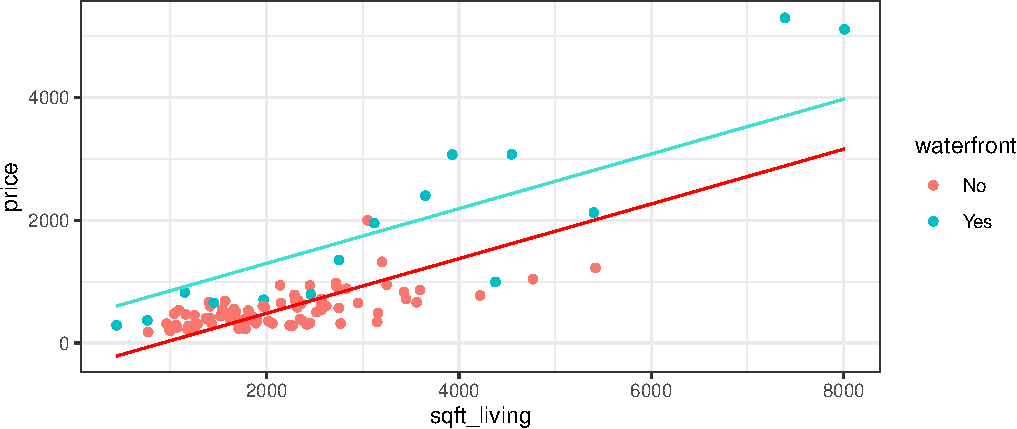
\includegraphics{Ch2_files/figure-pdf/unnamed-chunk-44-1.pdf}

This assumption of the rate of change in price with respect to living
space being the same for waterfront houses, as for non-waterfront houses
might be unrealistic.

Let's fit separate lines waterfront and non-waterfront houses, without
requiring them to have the same slope.

\begin{Shaded}
\begin{Highlighting}[]
\FunctionTok{ggplot}\NormalTok{(}\AttributeTok{data=}\NormalTok{Houses, }\FunctionTok{aes}\NormalTok{(}\AttributeTok{x=}\NormalTok{sqft\_living, }\AttributeTok{y=}\NormalTok{price, }\AttributeTok{color=}\NormalTok{waterfront)) }\SpecialCharTok{+} \FunctionTok{geom\_point}\NormalTok{()}\SpecialCharTok{+}\FunctionTok{stat\_smooth}\NormalTok{(}\AttributeTok{method=}\StringTok{"lm"}\NormalTok{, }\AttributeTok{se=}\ConstantTok{FALSE}\NormalTok{) }\SpecialCharTok{+} \FunctionTok{ylim}\NormalTok{(}\FunctionTok{c}\NormalTok{(}\DecValTok{0}\NormalTok{,}\DecValTok{5500}\NormalTok{)) }\SpecialCharTok{+} \FunctionTok{theme\_bw}\NormalTok{()}
\end{Highlighting}
\end{Shaded}

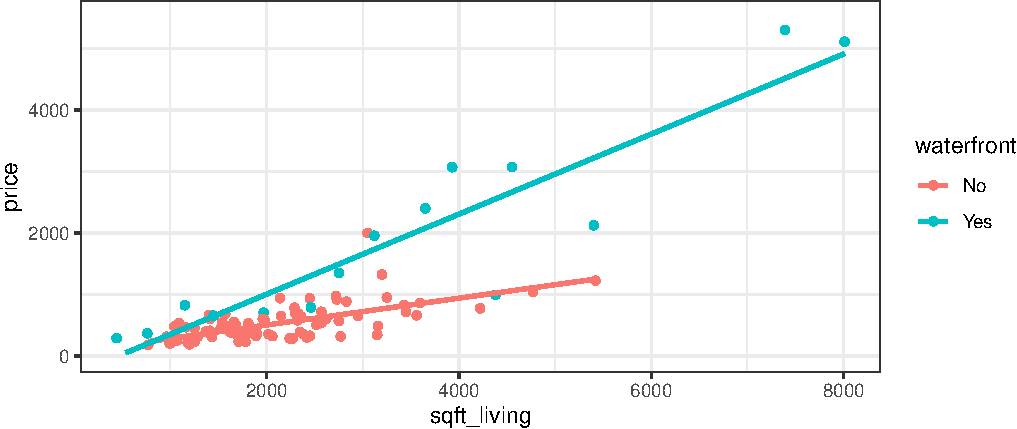
\includegraphics{Ch2_files/figure-pdf/unnamed-chunk-45-1.pdf}

It appears that the prices of the houses on the waterfront are
increasing more rapidly, with respect to square feet of living space,
than the non-waterfront houses. The effect of additional square feet on
the price of the house appears to depend on whether or not the house is
on the waterfront. This is an example of an \textbf{interaction} between
square footage and waterfront status.

An \textbf{interaction} between two explanatory variables occurs when
the effect of one explanatory variable on the response depends on the
other explanatory variable.

\subsection{Interaction Term}\label{interaction-term}

If we want to allow for different slopes between waterfront and
non-waterfront houses, we'll need to change the mathematical equation of
our model. To do that, we'll add a coefficient \(b_3\), multiplied by
the product of our two explanatory variables.

The model equation is

\[
\widehat{Price} = b_0 + b_1\times\text{Sq. Ft.} + b_2\times\text{waterfront} + b_3\times\text{Sq.Ft}\times\text{Waterfront}
\]

The last term is called an \textbf{interaction term.}

For a house on the waterfront (\(\text{waterfront}=1\)), the equation
relating price to square feet is

\[
\begin{aligned}
\widehat{Price} & = b_0 + b_1\times\text{Sq. Ft.} + b_2\times\text{1} + b_3\times\text{Sq.Ft}\times\text{1} \\
& = (b_0+b_2) + (b_1+b_3)\times{\text{Sq. Ft.}}
\end{aligned}
\] For a house not on the waterfront (\(\text{waterfront}=0\)), the
equation relating price to square feet is

\[
\begin{aligned}
\widehat{Price} & = b_0 + b_1\times\text{Sq. Ft.} + b_2\times\text{0} + b_3\times\text{Sq.Ft}\times\text{0} \\
& = b_0 + b_1\times{\text{Sq. Ft}}
\end{aligned}
\]

The intercept is \(b_0\) for non-waterfront houses, and \(b_0 + b_2\)
for waterfront houses.

The slope is \(b_1\) for non-waterfront houses, and \(b_1 + b_3\) for
waterfront houses.

Thus, the model allows both the slope and intercept to differ between
waterfront and non-waterfront houses.

\subsection{Interaction Models in R}\label{interaction-models-in-r}

To fit an interaction model in R, use \texttt{*} instead of \texttt{+}

\begin{Shaded}
\begin{Highlighting}[]
\NormalTok{M\_House\_Int }\OtherTok{\textless{}{-}} \FunctionTok{lm}\NormalTok{(}\AttributeTok{data=}\NormalTok{Houses, price}\SpecialCharTok{\textasciitilde{}}\NormalTok{sqft\_living}\SpecialCharTok{*}\NormalTok{waterfront)}
\NormalTok{M\_House\_Int}
\end{Highlighting}
\end{Shaded}

\begin{verbatim}

Call:
lm(formula = price ~ sqft_living * waterfront, data = Houses)

Coefficients:
              (Intercept)                sqft_living  
                  67.3959                     0.2184  
            waterfrontYes  sqft_living:waterfrontYes  
                -364.5950                     0.4327  
\end{verbatim}

The regression equation is

\[
\widehat{Price} = 67.4 + 0.2184\times\text{Sq. Ft.}  -364.6\times\text{waterfront} + 0.4327\times\text{Sq.Ft}\times\text{Waterfront}
\]

For a house on the waterfront (\(\text{waterfront}=1\)), the equation is

\[
\begin{aligned}
\widehat{Price} & = 67.4 + 0.2184\times\text{Sq. Ft.} -364.6 \times\text{1} + 0.4327\times\text{Sq.Ft}\times\text{1} \\
& = (67.4 - 364.6) + (0.2184+0.4327)\times{\text{Sq. Ft.}} \\
& = -297.2 + 0.6511\times{\text{Sq. Ft.}}
\end{aligned}
\] For a house not on the waterfront (\(\text{waterfront}=0\)), the
equation is

\[
\begin{aligned}
\widehat{Price} & = 67.4 + 0.2184\times\text{Sq. Ft.} -364.6 \times\text{0} + 0.4327\times\text{Sq.Ft}\times\text{0} \\
& = 67.4 0 + 0.2184\times{\text{Sq. Ft.}} 
\end{aligned}
\] \textbf{Interpretation}

When interpreting \(b_0\) and \(b_1\), we need to state that the
interpretations apply only to the ``baseline'' category (in this case
non-waterfront houses).

In a model with interaction, it does not make sense to talk about
holding one variable constant when interpreting the effect of the other,
since the effect of one variable depends on the value or category of the
other. Instead, we must state the value or category of one variable when
interpreting the effect of the other.

\textbf{Interpretations:}

\begin{itemize}
\item
  \(b_0\) - On average, a house with 0 square feet that is not on the
  waterfront is expected to cost 67 thousand dollars. This is not a
  sensible interpretation since there are no houses with 0 square feet.
\item
  \(b_1\) - For each additional square foot in size, the price of a
  non-waterfront house is expected to increase by 0.2184 thousand
  dollars.
\item
  \(b_2\) - On average, the price of a waterfront house with 0 square
  feet is expected to be 364.6 thousand dollars less than the price of a
  non-waterfront house with 0 square feet. This is not a sensible
  interpretation in this case.
\item
  \(b_3\) - For each additional square foot in size, the price of a
  waterfront house is expected to increase by 0.4327 thousand dollars
  more than a non-waterfront house.
\end{itemize}

Alternatively, we could interpret \(b_0+b_2\) and \(b_1+b_3\) together.

\begin{itemize}
\item
  \(b_0 + b_2\) - On average, a house with 0 square feet that is on the
  waterfront is expected to cost -297.2 thousand dollars. This is not a
  sensible interpretation since there are no houses with 0 square feet.
\item
  \(b_1\) - For each additional square foot in size, the price of a
  waterfront house is expected to increase by 0.6511 thousand dollars.
\end{itemize}

\textbf{Prediction}

We calculate predicted prices for the following houses:

\begin{Shaded}
\begin{Highlighting}[]
\NormalTok{Houses[}\FunctionTok{c}\NormalTok{(}\DecValTok{1}\NormalTok{,}\DecValTok{16}\NormalTok{), ] }\SpecialCharTok{\%\textgreater{}\%} \FunctionTok{select}\NormalTok{(Id, price, sqft\_living, waterfront)}
\end{Highlighting}
\end{Shaded}

\begin{verbatim}
# A tibble: 2 x 4
     Id price sqft_living waterfront
  <int> <dbl>       <dbl> <fct>     
1     1  1225        5420 No        
2    16  3075        4550 Yes       
\end{verbatim}

\[
\widehat{Price}_1 = 67.4 + 0.2184\times5420  -364.6\times0 + 0.4327\times5420 \times 0 = 1191 \text{ thousand dollars}
\]

\[
\widehat{Price}_{16} = 67.4 + 0.2184\times4450  -364.6\times1 + 0.4327\times4450 \times 1 = 2600 \text{ thousand dollars}
\]

\subsection{\texorpdfstring{\(R^2\) for Interaction
Model}{R\^{}2 for Interaction Model}}\label{r2-for-interaction-model}

We can calculate residuals, as well as SSR, SSM, SST, and \(R^2\), in
the same manner we've seen previously.

We'll perform these calculations using R.

\begin{Shaded}
\begin{Highlighting}[]
\NormalTok{SSR\_int }\OtherTok{\textless{}{-}} \FunctionTok{sum}\NormalTok{(M\_House\_Int}\SpecialCharTok{$}\NormalTok{residuals}\SpecialCharTok{\^{}}\DecValTok{2}\NormalTok{)}
\NormalTok{SSR\_int}
\end{Highlighting}
\end{Shaded}

\begin{verbatim}
[1] 10139974
\end{verbatim}

\[
SSM = SST-SSR = 69,045,634 - 10,139,974 =58,905,660.
\]

\[
R^2 = \frac{58,905,660}{69,045,634}=0.8531.
\]

Approximately 85.3\% of the total variability in sale price is explained
by the model using square feet and waterfront status, as well as an
interaction between them as the explanatory variables.

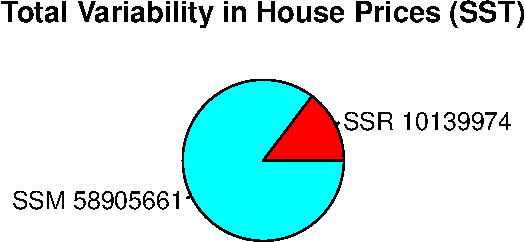
\includegraphics{Ch2_files/figure-pdf/unnamed-chunk-49-1.pdf}

We calculate \(R^2\) directly in R.

\begin{Shaded}
\begin{Highlighting}[]
\FunctionTok{summary}\NormalTok{(M\_House\_Int)}\SpecialCharTok{$}\NormalTok{r.squared}
\end{Highlighting}
\end{Shaded}

\begin{verbatim}
[1] 0.853141
\end{verbatim}

We see that adding an interaction term improved the proportion of
variability in house price explained by the model from 0.76 to 0.85.
This is a fairly notable increase.

\subsection{Considerations for Using
Interactions}\label{considerations-for-using-interactions}

It might be tempting to think we should always add an interaction term
to a model when using two or more explanatory variables. After all, an
interaction term is just another term added to the model, meaning that
\(R^2\) will never go down.

Adding an interaction term is not always a good idea, though. We saw
that doing so makes interpretations more complicated. Increasing the
complexity of a model also increases the risk of overfitting,
potentially hurting predictive performance on new data.

We should only add an interaction term if we have strong reason to
believe that the rate of change in the response variable with respect to
one explanatory variable really does depend on the other variable. This
might come from background knowledge about the subject, or consultation
with an expert in the area. It could also come from data visualization,
and the increase in variability in the response variable explained when
an interaction term is added to the model.

In the house price dataset, we might expect that the price of waterfront
houses might increase more rapidly as they get bigger than the price of
non-waterfront houses. The fact that the lines shown in the scatterplot
are not close to being parallel provides further evidence of a
difference in rate of increase, providing justification for the use of
an interaction term in the model. Furthermore, \(R^2\) increases notably
(from 0.76 to 0.85), when an interaction term is added. All of these
reasons support using an interaction term in this context.

When examining a scatterplot, we should note that even if there is truly
no interaction among all houses, the lines probably won't be exactly
parallel, due to random deviations among the sample of houses chosen. If
the lines are reasonably close to parallel, then an interaction term is
likely not needed.

We'll look more at criteria for determining whether to add an
interaction term to a model in the coming sections.

\subsection{Interaction vs
Correlation}\label{interaction-vs-correlation}

It is easy to confuse the concept of interaction with that of
correlation. These are, in fact, very different concepts.

A correlation between two variables means that as one increases, the
other is more likely to increase or decrease. We only use the word
correlation to describe two quantitative variables, but we could discuss
the similar notion of a relationship between categorical variables.

An interaction between two explanatory variables means that the effect
of one on the response depends on the other.

\textbf{Examples of Correlations (or relationships)}

\begin{enumerate}
\def\labelenumi{\arabic{enumi}.}
\item
  Houses on the waterfront tend to be bigger than houses not on the
  waterfront, so there is a relationship between square feet and
  waterfront status.
\item
  Houses with large amounts of living space in square feet are likely to
  have more bedrooms, so there is a correlation between living space and
  bedrooms.
\item
  Suppose that some genres of movies (drama, comedy, action, etc.) tend
  to be longer than others. This is an example of a relationship between
  genre and length.
\end{enumerate}

The fact that there is a correlation between explanatory variables is
NOT a reason to add an interaction term involving those variables in a
model. Correlation is something entirely different than interaction!

\textbf{Examples of Interactions}

\begin{enumerate}
\def\labelenumi{\arabic{enumi}.}
\item
  As houses on the waterfront increase in size, their price increases
  more rapidly than for houses not on the waterfront. This means there
  is an interaction between size and waterfront location.
\item
  Suppose that the effect of additional bedrooms on price is different
  for houses with lots of living space than for houses with little
  living space. This would be an example of an interaction between
  living space and number of bedrooms.
\item
  Suppose that audiences become more favorable to dramas as they get
  longer, but less favorable to comedies as they get longer. In this
  scenario, the effect of movie length on audience rating depends on the
  genre of the movie, indicating an interaction between length and
  genre.
\end{enumerate}

\section{Least Squares Estimation
(LSE)}\label{least-squares-estimation-lse}

\subsection{Estimating Regression
Coefficients}\label{estimating-regression-coefficients}

We've already used R to determine the estimates of \(b_0\), \(b_1\),
\(b_2\), and \(b_3\) in various kinds of linear models. At this point,
it is natural to wonder where these estimates are come from.

Regression coefficients \(b_0, b_1, \ldots, b_p\) are chosen in a way
that minimizes the sum of the squared differences between the observed
and predicted values. That is, we minimize

\[
\text{SSR} = \displaystyle\sum_{i=1}^{n} (y_i-\hat{y}_i)^2
\]

Because \(\hat{y}_i\) is a function of \(b_0, b_1, \ldots, b_p\), we can
choose the values of \(b_0, b_1, \ldots, b_p\) in a way that minimizes
SSR.

\[\text{SSR} = \displaystyle\sum_{i=1}^n (y_i -\hat{y}_i)^2  = \displaystyle\sum_{i=1}^n (y_i -(b_0 + b_1x_{i1} + b_2x_{i2} + \ldots + b_px_{ip}))^2 \]

The process of estimating regression coefficients
\(b_0, b_1, \ldots, b_p\) in a way that minimizes SSR is called
\textbf{least-squares estimation}.

\textbf{Example: Model with one quantitative variable}

We start with an example of estimating the regression coefficients for a
model with a single explanatory variable. This is easy to illustrate,
since we can draw a scatter plot displaying our explanatory and response
variable.

The figure below illustrates four possible trend lines that could be fit
to a set of 10 points in a scatter plot. The first line is the line of
best fit, in that it makes the sum of the squared residuals the smallest
of all possible lines that could be drawn. The second through fourth
plots all show examples of other trend lines that are not the line of
best fit. The sum of squared residuals for each of these models is
bigger than for the first one.

In the illustration, SSR is represented by the total area of the
squares. The line of best fit is the one that make the intercept the
smallest.

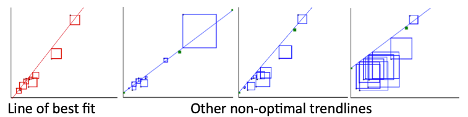
\includegraphics[width=1\textwidth,height=\textheight]{LSE.png}

\begin{itemize}
\tightlist
\item
  This
  \href{http://www.rossmanchance.com/applets/RegShuffle.htm}{Rossman-Chance
  applet} provides an illustration of the line of best fit.
\end{itemize}

Returning to the model for predicting price of a house, using only size
in square feet as an explanatory variable, the scatter plot, along with
the slope and intercept of the regression line are shown below.

\begin{Shaded}
\begin{Highlighting}[]
\FunctionTok{ggplot}\NormalTok{(}\AttributeTok{data=}\NormalTok{Houses, }\FunctionTok{aes}\NormalTok{(}\AttributeTok{x=}\NormalTok{sqft\_living, }\AttributeTok{y=}\NormalTok{price)) }\SpecialCharTok{+} \FunctionTok{geom\_point}\NormalTok{() }\SpecialCharTok{+} 
  \FunctionTok{stat\_smooth}\NormalTok{(}\AttributeTok{method=}\StringTok{"lm"}\NormalTok{, }\AttributeTok{se=}\ConstantTok{FALSE}\NormalTok{) }\SpecialCharTok{+} \FunctionTok{theme\_bw}\NormalTok{()}
\end{Highlighting}
\end{Shaded}

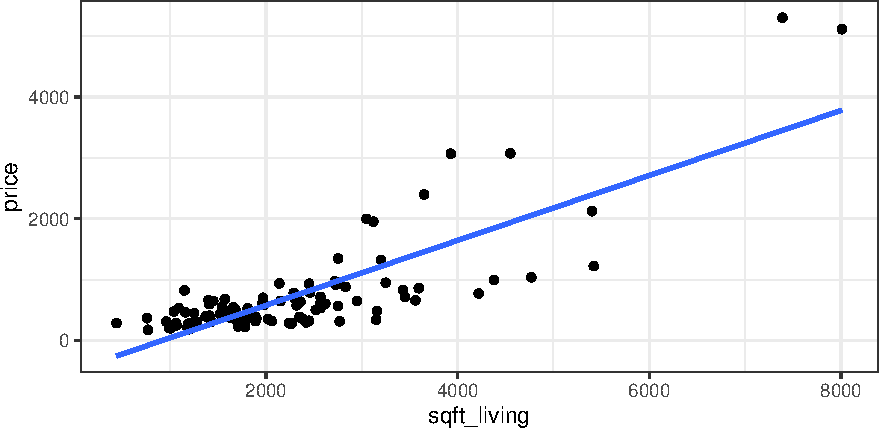
\includegraphics{Ch2_files/figure-pdf/unnamed-chunk-52-1.pdf}

\begin{Shaded}
\begin{Highlighting}[]
\NormalTok{M\_House\_sqft}
\end{Highlighting}
\end{Shaded}

\begin{verbatim}

Call:
lm(formula = price ~ sqft_living, data = Houses)

Coefficients:
(Intercept)  sqft_living  
  -484.9575       0.5328  
\end{verbatim}

The line \(\text{Price} = -485 + 0.5328 \times \text{Square Feet}\) is
the ``line of best fit'' in the sense that it minimizes the sum of the
squared residuals (SSR). Any other choices for the slope or intercept of
the regression line would result in larger SSR than this line.

\subsection{Mathematics of LSE for
SLR}\label{mathematics-of-lse-for-slr}

\begin{itemize}
\item
  Consider a \textbf{simple linear regression(SLR)} model, which is one
  with a singe quantitative explanatory variable \(x\).
\item
  \(\hat{y}_i = b_0+b_1x_i\)
\item
  we need to choose the values of \(b_0\) and \(b_1\) that minimize:
\end{itemize}

\[
\displaystyle\sum_{i=1}^n(y_i-\hat{y}_i)^2 =\displaystyle\sum_{i=1}^n(y_i-(b_0+b_1x_i))^2
\]

We setup the equation by substituting in the values of \(y_i\) and
\(x_i\) seen in the data.

Recall the first 3 houses in the dataset:

\begin{Shaded}
\begin{Highlighting}[]
\FunctionTok{kable}\NormalTok{(First3Houses)}
\end{Highlighting}
\end{Shaded}

\begin{longtable}[]{@{}rrlr@{}}
\toprule\noalign{}
Id & price & waterfront & sqft\_living \\
\midrule\noalign{}
\endhead
\bottomrule\noalign{}
\endlastfoot
1 & 1225 & No & 5420 \\
2 & 885 & No & 2830 \\
3 & 385 & No & 1620 \\
\end{longtable}

\[
\begin{aligned}
\displaystyle\sum_{i=1}^{100}(y_i-\hat{y}_i)^2 & =\displaystyle\sum_{i=1}^n(y_i-(b_0+b_1x_i))^2 \\
& = (1225-(b_0+b_1(5420)))^2 + (885-(b_0+b_1(2830)))^2 + (385-(b_0+b_1(1620)))^2 + \ldots
\end{aligned}
\]

We need to find the values of \(b_0\) and \(b_1\) that minimize this
expression. This is a 2-dimensional optimization problem that can be
solved using multivariable calculus or numerical or graphical methods.

Using calculus, it can be shown that this quantity is minimized when

\begin{itemize}
\item
  \(b_1=\frac{\displaystyle\sum_{i=1}^{n}(x_i-\bar{x})(y_i-\bar{y})}{\displaystyle\sum_{i=1}^{n}(x_i-\bar{x})^2}=\frac{\displaystyle\sum_{i=1}^{n} x_i y_i-\frac{\displaystyle\sum_{i=1}^{n} x_i \displaystyle\sum_{i=1}^{n} y_i }{n}}{\left(\displaystyle\sum_{i=1}^{n} x_i^2 -\frac{\left(\displaystyle\sum_{i=1}^{n} x_i\right)^2}{n}\right)}\)
\item
  \(b_0=\bar{y}-b_1\bar{x}\) (where
  \(\bar{y}=\frac{\displaystyle\sum_{i=1}^{n}{y_i}}{n}\), and
  \(\bar{x}=\frac{\displaystyle\sum_{i=1}^{n}{x_i}}{n}\)).
\end{itemize}

\subsection{LSE for Categorical
Variable}\label{lse-for-categorical-variable}

\begin{itemize}
\item
  Consider a model with a single categorical variable (such as
  waterfront), with G+1 categories, numbered \(g=0,2, \ldots, G\)
\item
  Then \(\hat{y}_i = b_0 + b_1x_{i1} + \ldots +b_{G}x_{iG}\).
\item
  we need to minimize
\end{itemize}

\[
\displaystyle\sum_{i=1}^n(y_i-\hat{y}_i)^2 =\displaystyle\sum_{i=1}^n(y_i-(b_0 + b_1x_{i1} + \ldots +b_{G}x_{iG}))^2.   
\]

\begin{itemize}
\tightlist
\item
  It can be shown that this is achieved when

  \begin{itemize}
  \tightlist
  \item
    \(b_0 = \bar{y_0}\) (i.e.~the average response in the ``baseline
    group''), and\\
  \item
    \(b_j = \bar{y_j} - \bar{y}_0\)
  \end{itemize}
\end{itemize}

\subsection{LSE More Generally}\label{lse-more-generally}

\begin{itemize}
\tightlist
\item
  For multiple regression models, including those involving interaction,
  the logic is the same. We need to choose \(b_0, b_1, \ldots, b_p\) in
  order to minimize
\end{itemize}

\[ \displaystyle\sum_{i=1}^n (y_i -\hat{y}_i)^2  = \displaystyle\sum_{i=1}^n (y_i -(b_0 + b_1x_{i1} + b_2x_{i2} + \ldots + b_px_{ip}))^2 \]

\begin{itemize}
\item
  The mathematics, however, are more complicated and require inverting a
  matrix. This goes beyond the scope of this class, so we will let R do
  the estimation and use the results.
\item
  More on least squares estimation in multiple regression can be found
  \href{http://www.math.chalmers.se/Stat/Grundutb/GU/MSG500/A10/lecture5.pdf}{here}.
\end{itemize}

\section{ANalysis Of VAriance}\label{analysis-of-variance}

\subsection{Submodels}\label{submodels}

We've seen 5 different models for predicting house price using some
combination of square feet and waterfront status.

A model A is defined to be a \textbf{submodel} of another model B, if
every term in model A is also included in model B.

\begin{longtable}[]{@{}
  >{\raggedright\arraybackslash}p{(\columnwidth - 8\tabcolsep) * \real{0.0511}}
  >{\raggedright\arraybackslash}p{(\columnwidth - 8\tabcolsep) * \real{0.2774}}
  >{\raggedright\arraybackslash}p{(\columnwidth - 8\tabcolsep) * \real{0.1898}}
  >{\raggedright\arraybackslash}p{(\columnwidth - 8\tabcolsep) * \real{0.2190}}
  >{\raggedright\arraybackslash}p{(\columnwidth - 8\tabcolsep) * \real{0.2628}}@{}}
\toprule\noalign{}
\begin{minipage}[b]{\linewidth}\raggedright
Model
\end{minipage} & \begin{minipage}[b]{\linewidth}\raggedright
Variables
\end{minipage} & \begin{minipage}[b]{\linewidth}\raggedright
Unexplained Variability
\end{minipage} & \begin{minipage}[b]{\linewidth}\raggedright
Variability Explained
\end{minipage} & \begin{minipage}[b]{\linewidth}\raggedright
\(R^2\)
\end{minipage} \\
\midrule\noalign{}
\endhead
\bottomrule\noalign{}
\endlastfoot
0 & None & 69045634 & 0 & 0 \\
1 & Sq. Ft. & 23767280 & 45278354 & 0.656 \\
2 & Waterfront & 43675043 & 25370591 & 0.367 \\
3 & Sq. Ft. and Waterfront & 16521296 & 52524338 & 0.761 \\
4 & Sq. Ft., Waterfront, and Interaction & 10139974 & 58905661 &
0.853 \\
\end{longtable}

\begin{itemize}
\item
  Model 1 is a submodel of Model 3, since all variables used in Model 1
  are also used in Model 3.
\item
  Model 2 is also a submodel of Model 3.
\item
  Models 1, 2, and 3 are all submodels of Model 4.
\item
  Model 0 is a submodel of Models 1, 2, 3, and 4.
\item
  Models 1 and 2 are not submodels of each other, since Model 1 contains
  a variable used in Model 2 and Model 2 contains a variable not used in
  Model 1.
\end{itemize}

\subsection{F-Statistics}\label{f-statistics}

When one model is a submodel of another, we can compare the amount of
variability explained by the models, using a technique known as
\textbf{ANalysis Of VAriance (ANOVA)}.

Reduced Model:
\(\hat{y}_i = b_0 + b_1x_{i1} + b_2x_{i2} + \ldots + b_qx_{iq}\)

Full Model:
\(\hat{y}_i = b_0 + b_1x_{i1} + b_2x_{i2} + \ldots + b_qx_{iq} + b_{q+1}x_{i{q+1}} \ldots + b_px_{ip}\)

p = \# terms in Full Model, not including the intercept\\
q = \# terms in Reduced Model, not including the intercept\\
n = number of observations

We calculate a statistic called F that measures the amount of
variability explained by adding additional variable(s) to the model,
relative to the total amount of unexplained variability.

\[
\begin{aligned}
F  
&= \frac{\frac{\text{SSR}_{\text{Reduced}}-\text{SSR}_{\text{Full}}}{p-q}}{\frac{\text{SSR}_{\text{Full}}}{n-(p+1)}}
\end{aligned}
\]

\begin{itemize}
\tightlist
\item
  Large values of F indicate that adding the additional explanatory
  variables is helpful in explaining variability in the response
  variable\\
\item
  Small values of F indicate that adding new explanatory variables
  variables does not make much of a difference in explaining variability
  in the response variable\\
\item
  What counts as ``large'' is depends on \(n, p,\) and \(q\). We will
  revisit this later in the course.
\end{itemize}

\textbf{Example 1}

Let's Calculate an ANOVA F-Statistic to compare Models 1 and 3.

Reduced Model:

\[
\widehat{\text{Price}}= b_0+ b_1 \times\text{sqft\_living}
\]

Full Model:

\[
\widehat{\text{Price}}= b_0+ b_1 \times\text{sqft\_living}+ b_2\times\text{Waterfront}
\]

\[
\begin{aligned}
F &= \frac{\frac{\text{SSR}_{\text{Reduced}}-\text{SSR}_{\text{Full}}}{p-q}}{\frac{\text{SSR}_{\text{Full}}}{n-(p+1)}} \\
&=\frac{\frac{23,767,280-16,521,296}{2-1}}{\frac{16,521,296}{100-(2+1)}} \\
\end{aligned}
\]

\begin{Shaded}
\begin{Highlighting}[]
\NormalTok{((SSR\_sqft}\SpecialCharTok{{-}}\NormalTok{SSR\_wf\_sqft)}\SpecialCharTok{/}\NormalTok{(}\DecValTok{2{-}1}\NormalTok{))}\SpecialCharTok{/}\NormalTok{((SSR\_wf\_sqft)}\SpecialCharTok{/}\NormalTok{(}\DecValTok{100}\SpecialCharTok{{-}}\NormalTok{(}\DecValTok{2}\SpecialCharTok{+}\DecValTok{1}\NormalTok{)))}
\end{Highlighting}
\end{Shaded}

\begin{verbatim}
[1] 42.54269
\end{verbatim}

We can calculate the statistic directly in R, using the \texttt{anova}
command.

\begin{Shaded}
\begin{Highlighting}[]
\FunctionTok{anova}\NormalTok{(M\_House\_sqft, M\_wf\_SqFt)}\SpecialCharTok{$}\NormalTok{F[}\DecValTok{2}\NormalTok{]}
\end{Highlighting}
\end{Shaded}

\begin{verbatim}
[1] 42.54269
\end{verbatim}

In the coming chapters, we'll talk about what to conclude from an
F-statistic of 42.5 Is this big enough to say that adding waterfront
status to a model already including square feet helps better explain
variability in sale price? (Spoiler alert: YES - an F-statistic of 42.5
is quite large and indicative that the full model is a better choice
than the reduced model.) We previously saw that the model including both
square feet and waterfront status had a \(R^2\) value considerably
higher than the one including only square feet. This large F-statistic
is further evidence to the benefit of considering both variables in our
model.

\textbf{Example 2}

We'll calculate an F-statistic to compare Models 3 and 4. This can help
us determine whether it is worthwhile to include an interaction term in
our model.

Reduced Model:
\[\widehat{\text{Price}}= b_0+ b_1 \times\text{sqft\_living} + b_2\times\text{Waterfront}\]

Full Model:
\[\widehat{\text{Price}}= b_0+ b_1 \times\text{sqft\_living}+ b_2\times\text{Waterfront} + b_3\times\text{sqft\_living}\times\text{Waterfront}\]

\[
\begin{aligned}
F &= \frac{\frac{\text{SSR}_{\text{Reduced}}-\text{SSR}_{\text{Full}}}{p-q}}{\frac{\text{SSR}_{\text{Full}}}{n-(p+1)}} \\
&=\frac{\frac{16,521,296-10,139,974}{3-2}}{\frac{10,139,974}{100-(3+1)}} \\
\end{aligned}
\]

\begin{Shaded}
\begin{Highlighting}[]
\NormalTok{((SSR\_wf\_sqft}\SpecialCharTok{{-}}\NormalTok{SSR\_int)}\SpecialCharTok{/}\NormalTok{(}\DecValTok{3{-}2}\NormalTok{))}\SpecialCharTok{/}\NormalTok{((SSR\_int)}\SpecialCharTok{/}\NormalTok{(}\DecValTok{100}\SpecialCharTok{{-}}\NormalTok{(}\DecValTok{3}\SpecialCharTok{+}\DecValTok{1}\NormalTok{)))}
\end{Highlighting}
\end{Shaded}

\begin{verbatim}
[1] 60.41505
\end{verbatim}

We can calculate the statistic directly in R, using the \texttt{anova}
command.

\begin{Shaded}
\begin{Highlighting}[]
\FunctionTok{anova}\NormalTok{(M\_wf\_SqFt, M\_House\_Int)}\SpecialCharTok{$}\NormalTok{F[}\DecValTok{2}\NormalTok{]}
\end{Highlighting}
\end{Shaded}

\begin{verbatim}
[1] 60.41505
\end{verbatim}

We observe an F-statistic of 60, which is even bigger than the one seen
previously! This suggests that adding the interaction term does indeed
improve the model's ability to account for variability in prices.

\subsection{Comparing 3 or More
Categories}\label{comparing-3-or-more-categories}

F-statistics are commonly used when making comparisons involving
categorical variables with 3 or more categories.

One variable in the houses dataset, which we haven't looked at yet, is
the condition of the house at the time of sale. The table shows the
number of houses in each condition listed.

\begin{Shaded}
\begin{Highlighting}[]
\FunctionTok{summary}\NormalTok{(Houses}\SpecialCharTok{$}\NormalTok{condition)}
\end{Highlighting}
\end{Shaded}

\begin{verbatim}
average or below             good        very_good 
              61               30                9 
\end{verbatim}

We notice that there is only one house in poor condition and one house
in fair condition. These sample sizes are too small to analyze. We'll
combine these two houses with those in the ``average'' category,
creating a new category called ``average or below).

\begin{Shaded}
\begin{Highlighting}[]
\NormalTok{Houses}\SpecialCharTok{$}\NormalTok{condition }\OtherTok{\textless{}{-}} \FunctionTok{fct\_collapse}\NormalTok{(Houses}\SpecialCharTok{$}\NormalTok{condition, }\StringTok{"average or below"} \OtherTok{=} \FunctionTok{c}\NormalTok{(}\StringTok{"poor"}\NormalTok{,}\StringTok{"fair"}\NormalTok{, }\StringTok{"average"}\NormalTok{))}
\end{Highlighting}
\end{Shaded}

The boxplot shows the distribution of houses in each category, and the
table below it provides a numerical summary.

\begin{Shaded}
\begin{Highlighting}[]
\FunctionTok{ggplot}\NormalTok{(}\AttributeTok{data=}\NormalTok{Houses, }\FunctionTok{aes}\NormalTok{(}\AttributeTok{x=}\NormalTok{condition, }\AttributeTok{y=}\NormalTok{price)) }\SpecialCharTok{+} \FunctionTok{geom\_boxplot}\NormalTok{() }\SpecialCharTok{+}\FunctionTok{coord\_flip}\NormalTok{()}
\end{Highlighting}
\end{Shaded}

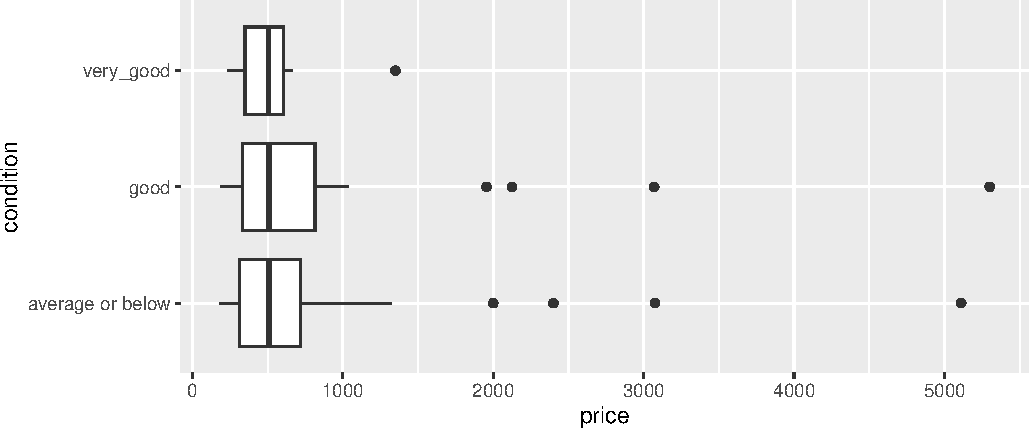
\includegraphics{Ch2_files/figure-pdf/unnamed-chunk-61-1.pdf}

\begin{Shaded}
\begin{Highlighting}[]
\NormalTok{Cond\_Tab }\OtherTok{\textless{}{-}}\NormalTok{ Houses }\SpecialCharTok{\%\textgreater{}\%} \FunctionTok{group\_by}\NormalTok{(condition) }\SpecialCharTok{\%\textgreater{}\%} \FunctionTok{summarize}\NormalTok{(}\AttributeTok{Mean\_Price =} \FunctionTok{mean}\NormalTok{(price), }
                                             \AttributeTok{SD\_Price=} \FunctionTok{sd}\NormalTok{ (price), }
                                             \AttributeTok{N=} \FunctionTok{n}\NormalTok{())}
\FunctionTok{kable}\NormalTok{(Cond\_Tab)}
\end{Highlighting}
\end{Shaded}

\begin{longtable}[]{@{}lrrr@{}}
\toprule\noalign{}
condition & Mean\_Price & SD\_Price & N \\
\midrule\noalign{}
\endhead
\bottomrule\noalign{}
\endlastfoot
average or below & 700.6349 & 768.1179 & 61 \\
good & 861.0000 & 1048.9521 & 30 \\
very\_good & 551.8361 & 332.8597 & 9 \\
\end{longtable}

It can be helpful to calculate a single statistic that quantifies the
size of the differences between the conditions. If we were just
comparing two different categories, we could simply find the difference
in mean prices between them. But, with three or more categories, we need
a way to represent the size of the differences with a single number. An
F-statistic can serve this purpose.

We'll calculate an F-statistic for a model that includes condition,
compared to a model with only an intercept term.

Reduced Model: \[\widehat{\text{Price}}= b_0\]

Full Model:
\[\widehat{\text{Price}}= b_0+ b_1 \times\text{good condition}+ b_2\times\text{very good condition}\]

Notice that the equation includes separate variables for the ``good''
and ``very'' good conditions. These variables take on value 0 if the
house is not in that condition, and 1 if the house is in that condition.
Here, houses in ``average or below'' condition are considered the
``baseline'' category.

We'll fit the model in R. The coefficient estimates for \(b_0\), \(b_1\)
and \(b_2\) are shown below.

\begin{Shaded}
\begin{Highlighting}[]
\NormalTok{M\_House\_Cond }\OtherTok{\textless{}{-}} \FunctionTok{lm}\NormalTok{(}\AttributeTok{data=}\NormalTok{Houses, price}\SpecialCharTok{\textasciitilde{}}\NormalTok{condition)}
\NormalTok{M\_House\_Cond}
\end{Highlighting}
\end{Shaded}

\begin{verbatim}

Call:
lm(formula = price ~ condition, data = Houses)

Coefficients:
       (Intercept)       conditiongood  conditionvery_good  
             700.6               160.4              -148.8  
\end{verbatim}

The model equation is

\[
\widehat{\text{Price}}= b_0+ b_1 \times\text{good condition}+ b_2\times\text{very good condition}
\]

\textbf{Interpretations}

\begin{itemize}
\tightlist
\item
  On average, houses in average or below condition cost 700.6 thousand
  dollars.\\
\item
  On average, houses in good condition cost 160.4 thousand dollars more
  than those in average or below condition.\\
\item
  On average, houses in very good condition cost 148.8 thousand dollars
  less than those in average or below condition.
\end{itemize}

This last sentence is surprising and merits further investigation. We'll
leave that for future consideration.

For now, we'll calculate an F-statistic based on the models.

Note that in this case, the reduced model does not include any
explanatory variables, so SSR is equal to SST, which we calculate
previously.

\begin{Shaded}
\begin{Highlighting}[]
\NormalTok{SST}
\end{Highlighting}
\end{Shaded}

\begin{verbatim}
[1] 69045634
\end{verbatim}

We calculate SSR for the full model.

\begin{Shaded}
\begin{Highlighting}[]
\NormalTok{SSR\_cond }\OtherTok{\textless{}{-}} \FunctionTok{sum}\NormalTok{(M\_House\_Cond}\SpecialCharTok{$}\NormalTok{residuals}\SpecialCharTok{\^{}}\DecValTok{2}\NormalTok{)}
\NormalTok{SSR\_cond  }
\end{Highlighting}
\end{Shaded}

\begin{verbatim}
[1] 68195387
\end{verbatim}

\[
\begin{aligned}
F &= \frac{\frac{\text{SSR}_{\text{Reduced}}-\text{SSR}_{\text{Full}}}{p-q}}{\frac{\text{SSR}_{\text{Full}}}{n-(p+1)}} \\
&=\frac{\frac{69,045,634-68,195,387}{2-0}}{\frac{68,195,387}{100-(2+1)}} \\
\end{aligned}
\]

\begin{Shaded}
\begin{Highlighting}[]
\NormalTok{((SST }\SpecialCharTok{{-}}\NormalTok{ SSR\_cond)}\SpecialCharTok{/}\NormalTok{(}\DecValTok{2{-}0}\NormalTok{))}\SpecialCharTok{/}\NormalTok{(SSR\_cond}\SpecialCharTok{/}\NormalTok{(}\DecValTok{100}\SpecialCharTok{{-}}\NormalTok{(}\DecValTok{2}\SpecialCharTok{+}\DecValTok{1}\NormalTok{)))}
\end{Highlighting}
\end{Shaded}

\begin{verbatim}
[1] 0.6046888
\end{verbatim}

We perform the calculation directly in R.

\begin{Shaded}
\begin{Highlighting}[]
\FunctionTok{anova}\NormalTok{(M\_House\_Cond, M0\_House)}\SpecialCharTok{$}\NormalTok{F[}\DecValTok{2}\NormalTok{]}
\end{Highlighting}
\end{Shaded}

\begin{verbatim}
[1] 0.6046888
\end{verbatim}

Notice that the F-statistic of 0.6 is considerably smaller than the
F-statistics we've seen previously.

This indicates that adding condition to a model with no other
explanatory variables doesn't seem to help improve the model's ability
to account for variation in price. Put another way, there doesn't appear
to be much evidence of difference in price between houses in the
different conditions.

\subsection{F-Statistic Illustration}\label{f-statistic-illustration}

The figure below gives an illustration of data that would produce a
large F-statistic (Scenario 1), and also data that would produce a small
F-statistic (Scenario 2), like the one seen in the house condition data.

An F-statistic compares the amount of variability between groups to the
amount of variability within groups.

In scenario 1, we notice considerable differences between the groups,
relative to the amount of variability within groups. In this scenario,
knowing the group an observation is in will help us predict the response
for that group, so we should include account for the groups in our
model. We would obtain a large F-statistic when comparing a model that
includes group to one that contains only an intercept term.

In scenario 2, there is little difference between the overall averages
in each group, and more variability between individual observations
within each group. In a scenario like this, knowing the group an
observation lies in does little to help us predict the response. In this
scenario, predictions from a model that includes group as an explantory
variable would not be much better than those from a model that does not.
Hence, we would obtain a small F-statistic.

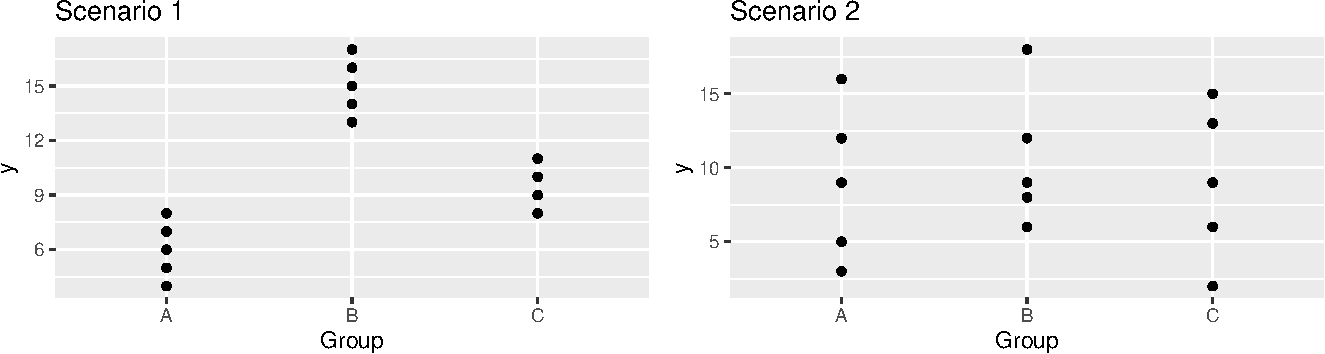
\includegraphics{Ch2_files/figure-pdf/unnamed-chunk-69-1.pdf}

\begin{longtable}[]{@{}
  >{\raggedright\arraybackslash}p{(\columnwidth - 4\tabcolsep) * \real{0.3059}}
  >{\raggedright\arraybackslash}p{(\columnwidth - 4\tabcolsep) * \real{0.3647}}
  >{\raggedright\arraybackslash}p{(\columnwidth - 4\tabcolsep) * \real{0.3294}}@{}}
\toprule\noalign{}
\begin{minipage}[b]{\linewidth}\raggedright
\end{minipage} & \begin{minipage}[b]{\linewidth}\raggedright
Scenario 1
\end{minipage} & \begin{minipage}[b]{\linewidth}\raggedright
Scenario 2
\end{minipage} \\
\midrule\noalign{}
\endhead
\bottomrule\noalign{}
\endlastfoot
variation between groups & High & Low \\
variation within groups & Low & High \\
F Statistic & Large & Small \\
Result & Evidence of Group Differences & No evidence of differences \\
\end{longtable}

\subsection{Alternative F-Statistic
Formula}\label{alternative-f-statistic-formula}

The above illustration suggests alternative (and mathematically
equivalent) way to calculate the F-statistic. We calculate the ratio of
variability between different groups, relative to the amount of
variability within each group

For a categorical variable with \(g\) groups,

\begin{itemize}
\item
  let \(\bar{y}_{1\cdot}, \ldots, \bar{y}_{g\cdot}\) represent the mean
  response for each group.
\item
  let \(n_1, \ldots, n_g\) represent the sample size for each group
\item
  Then
  \(\frac{\displaystyle\sum_{i=1}^g\sum_{j=1}^{n_i}n_i(y_{i\cdot}-\bar{y}_{\cdot\cdot})^2}{g-1}\)
  gives a measure of how much the group means differ, and
\item
  \(\frac{\displaystyle\sum_{i=1}^g\sum_{j=1}^{n_i}(y_{ij}-\bar{y}_{i\cdot})^2}{n-g}\)
  gives a measure of how much individual observations differ within
  groups
\item
  An alternative formula for this F-statistic is:
\end{itemize}

\[
F= \frac{\text{Variability between groups}}{\text{Variability within groups}}= \frac{\frac{\displaystyle\sum_{i=1}^g\sum_{j=1}^{n_i}n_i(y_{i\cdot}-\bar{y}_{\cdot\cdot})^2}{g-1}}{\frac{\displaystyle\sum_{i=1}^g\sum_{j=1}^{n_i}(y_{ij}-\bar{y}_{i\cdot})^2}{n-g}}
\]

\begin{itemize}
\tightlist
\item
  It can be shown that this statistic is equivalent to the one we saw
  previously.
\end{itemize}

\textbf{Example}

Let's recalculate the F-statistic for the conditions of the houses,
using this alternate formula. The first 3 houses are shown.

\begin{Shaded}
\begin{Highlighting}[]
\FunctionTok{kable}\NormalTok{(}\FunctionTok{head}\NormalTok{(Houses }\SpecialCharTok{\%\textgreater{}\%} \FunctionTok{select}\NormalTok{(Id, price, condition),}\DecValTok{3}\NormalTok{))}
\end{Highlighting}
\end{Shaded}

\begin{longtable}[]{@{}rrl@{}}
\toprule\noalign{}
Id & price & condition \\
\midrule\noalign{}
\endhead
\bottomrule\noalign{}
\endlastfoot
1 & 1225 & average or below \\
2 & 885 & average or below \\
3 & 385 & good \\
\end{longtable}

We have seen previously that:

\begin{itemize}
\tightlist
\item
  \(\bar{y}_{\cdot\cdot}=735.3526\) (overall average price), and
  \(n=10\)
\item
  \(\bar{y}_{1\cdot}=700.6349\) (average price for average or below
  houses), and \(n_1=61\)\\
\item
  \(\bar{y}_{2\cdot}=861.0\) (average price for good houses), and
  \(n_2=30\)\\
\item
  \(\bar{y}_{3\cdot}=551.8361\) (average price for very good houses),
  and \(n_3=9\)
\end{itemize}

Then,

\begin{itemize}
\item
  \(\frac{\displaystyle\sum_{i=1}^g\sum_{j=1}^{n_i}(y_{i\cdot}-\bar{y}_{\cdot\cdot})^2}{g-1} = \frac{61(700.6349-735.3526)^2+30(861.0-735.3526)^2+9(551.8361-735.3526)^2}{3-1} = \frac{850247.3}{2}\),
  and
\item
  \(\frac{\displaystyle\sum_{i=1}^g\sum_{j=1}^{n_i}(y_{ij}-\bar{y}_{i\cdot})^2}{n-g} = \frac{(1225.0-700.6349)^2+ (885.0 - 700.6349)^2 + (385.0-861.0)^2+\ldots}{100-3} = \frac{68195387}{97}\)
\end{itemize}

\[
F= \frac{\frac{\displaystyle\sum_{i=1}^g\sum_{j=1}^{n_i}n_i(y_{i\cdot}-\bar{y}_{\cdot\cdot})^2}{g-1}}{\frac{\displaystyle\sum_{i=1}^g\sum_{j=1}^{n_i}(y_{ij}-\bar{y}_{i\cdot})^2}{n-g}} = \frac{\frac{61(700.6349-735.3526)^2+30(861.0-735.3526)^2+9(551.8361-735.3526)^2}{3-1}}{\frac{(1225.0-700.6349)^2+ (885.0 - 700.6349)^2 + (385.0-861.0)^2+\ldots}{100-3}} = \frac{\frac{850247.3}{2}}{\frac{68195387}{97}}
\]

\begin{itemize}
\tightlist
\item
  Note that the quantity in the the quantity in the third line is
  equivalent to the sum of the squared residuals using M2. Thus, we can
  calculate F using:
\end{itemize}

\begin{Shaded}
\begin{Highlighting}[]
\NormalTok{((}\DecValTok{61}\SpecialCharTok{*}\NormalTok{(}\FloatTok{700.6349{-}735.3526}\NormalTok{)}\SpecialCharTok{\^{}}\DecValTok{2}\SpecialCharTok{+}\DecValTok{30}\SpecialCharTok{*}\NormalTok{(}\FloatTok{861.0{-}735.3526}\NormalTok{)}\SpecialCharTok{\^{}}\DecValTok{2}\SpecialCharTok{+}\DecValTok{9}\SpecialCharTok{*}\NormalTok{(}\FloatTok{551.8361{-}735.3526}\NormalTok{)}\SpecialCharTok{\^{}}\DecValTok{2}\NormalTok{)}\SpecialCharTok{/}\NormalTok{(}\DecValTok{3{-}1}\NormalTok{))}\SpecialCharTok{/}\NormalTok{((SSR\_cond)}\SpecialCharTok{/}\NormalTok{(}\DecValTok{100{-}3}\NormalTok{))}
\end{Highlighting}
\end{Shaded}

\begin{verbatim}
[1] 0.6046889
\end{verbatim}

For models with only one categorical explanatory variable, ``variability
within vs variability between'' interpretation of an F-statistic is very
popular. This statistic is often relevant in studies in the natural and
social sciences. Such studies are often referred to as One-Way ANOVA's.
In fact, these are just a special case of the full vs reduced model
interpretation of the F-statistic, which can be applied to any two
models, as long as one is a submodel of the other.

\bookmarksetup{startatroot}

\chapter{Simulation-Based Inference}\label{simulation-based-inference}

\textbf{Learning Outcomes:}

\begin{enumerate}
\def\labelenumi{\arabic{enumi}.}
\setcounter{enumi}{13}
\tightlist
\item
  Define population, sample, and sampling distribution, and a parameter
  and statistic.\\
\item
  Interpret standard deviation and standard error in context.\\
\item
  Explain how to use bootstrapping to calculate confidence intervals.\\
\item
  Interpret confidence intervals in context.\\
\item
  Calculate confidence intervals in R.
\item
  Write null and alternative hypotheses, identify test statistics, and
  state conclusions in context.\\
\item
  Interpret p-values in context.\\
\item
  Explain how to use simulation to perform hypothesis tests.
\item
  Compare and contrast the conclusions we can draw from confidence
  intervals and hypothesis tests.\\
\item
  Perform hypothesis tests in R.
\end{enumerate}

\section{Sampling Distributions}\label{sampling-distributions}

\subsection{Population and Sample}\label{population-and-sample}

In statistics, we often do not have the time, money, or means to collect
data on all individuals or units on which we want to draw conclusions.
Instead, we might collect data on only a subset of the individuals, and
then make inferences about all individuals we are interested in, using
the information we collected.

\textbf{Vocabulary:}

\begin{enumerate}
\def\labelenumi{\arabic{enumi}.}
\tightlist
\item
  A \textbf{population} is the entire set of individuals that we want to
  draw conclusions about.
\item
  A \textbf{sample} is a subset of a population.\\
\item
  A \textbf{parameter} is a numerical quantity pertaining to an entire
  population or process.\\
\item
  A \textbf{statistic} is a numerical quantity calculated from a sample.
\end{enumerate}

We'll work with a dataset containing information on all 20,591 flights
from New York to Chicago in 2013. Our population of interest is all
20,591 flights. We're interested in the proportion of fights that arrive
on time, and the average arrival delay (in minutes). Arrival delay
represents how much earlier/later did the flight arrive than expected.
Whether or not the flight arrived on time is a categorical variable,
while arrival delay is a quantitative variable.

In this situation, we have information on the entire population. In
statistics, this is rare. It is more common to have information on only
subset of flights contained in a sample. If the sample is collected in a
way that is representative of the population, such as by sampling at
random, then we can use the sample to draw conclusions about the
population.

We'll begin by studying the behavior of sample statistics when we know
the population parameters, and then use what we learn to handle more
real situations where we don't know about the entire population.

The parameter of interest is the proportion of on-time arrivals out of
all flights in the population of 20,591. When the parameter is
proportion, we'll denote it with the letter \(p\).

The first 10 flights, all of which occurred on January 1 are shown
below. We see that most of those flights were not on-time.

\begin{Shaded}
\begin{Highlighting}[]
\FunctionTok{head}\NormalTok{(Flights\_NY\_CHI, }\DecValTok{10}\NormalTok{)}
\end{Highlighting}
\end{Shaded}

\begin{verbatim}
# A tibble: 10 x 9
    year month   day carrier origin dest  sched_dep_time arr_delay ontime
   <int> <int> <int> <chr>   <chr>  <chr>          <int>     <dbl> <chr> 
 1  2013     1     1 UA      EWR    ORD              558        12 N     
 2  2013     1     1 AA      LGA    ORD              600         8 N     
 3  2013     1     1 MQ      EWR    ORD              600        32 N     
 4  2013     1     1 AA      LGA    ORD              630        14 N     
 5  2013     1     1 AA      LGA    ORD              700         4 N     
 6  2013     1     1 UA      LGA    ORD              700        20 N     
 7  2013     1     1 UA      EWR    ORD              713        21 N     
 8  2013     1     1 AA      LGA    ORD              745       -12 Y     
 9  2013     1     1 MQ      EWR    ORD              710        49 N     
10  2013     1     1 B6      JFK    ORD              830        15 N     
\end{verbatim}

Note that a negative arrival delay denotes a flight that arrived before
expected, thus on time.

The bar graph shows the number of flights that arrived on time
throughout the year.

\begin{Shaded}
\begin{Highlighting}[]
\NormalTok{on\_time\_plot\_POP }\OtherTok{\textless{}{-}} \FunctionTok{ggplot}\NormalTok{(}\AttributeTok{data=}\NormalTok{Flights\_NY\_CHI, }\FunctionTok{aes}\NormalTok{(}\AttributeTok{x=}\NormalTok{ontime)) }\SpecialCharTok{+} 
                  \FunctionTok{geom\_bar}\NormalTok{(}\AttributeTok{fill=}\StringTok{"blue"}\NormalTok{) }\SpecialCharTok{+} 
                  \FunctionTok{ggtitle}\NormalTok{(}\StringTok{"On{-}time Flights"}\NormalTok{)}
\NormalTok{on\_time\_plot\_POP}
\end{Highlighting}
\end{Shaded}

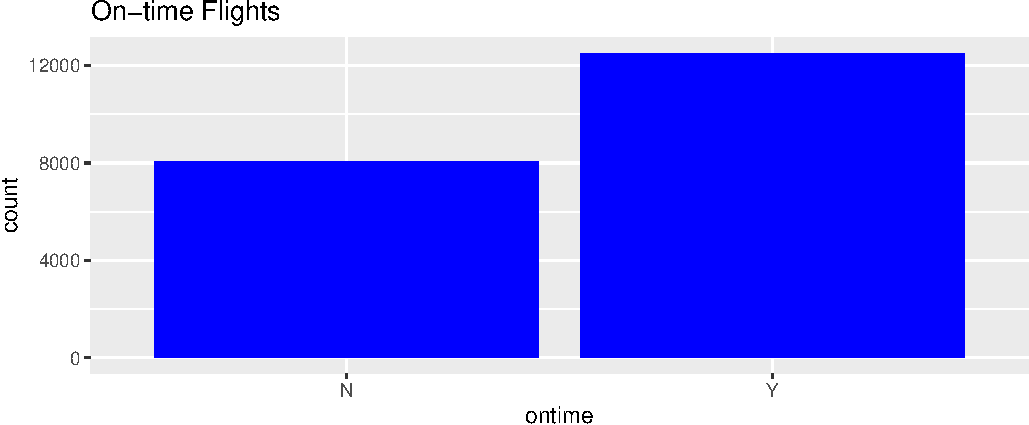
\includegraphics{Ch3_files/figure-pdf/unnamed-chunk-5-1.pdf}

We see that the majority of flights did arrive on time.

We'll calculate the proportion of flights arriving on time, among all
20,591 flights in the population.

\begin{Shaded}
\begin{Highlighting}[]
\CommentTok{\#proportion of flights on time}
\NormalTok{p }\OtherTok{\textless{}{-}} \FunctionTok{sum}\NormalTok{(Flights\_NY\_CHI}\SpecialCharTok{$}\NormalTok{ontime}\SpecialCharTok{==}\StringTok{"Y"}\NormalTok{)}\SpecialCharTok{/}\DecValTok{20591}
\NormalTok{p}
\end{Highlighting}
\end{Shaded}

\begin{verbatim}
[1] 0.6079841
\end{verbatim}

When the population parameter is a proportion, we'll denote it with the
letter \(p\). Here \$p=\$0.6079841. Keep in mind that in a real
situation, we typically won't know the value of the population parameter
\(p\), and will need to estimate it from a sample.

The histogram shows the distribution of arrival delay times. Negative
delays indicate the flight arriving ahead of schedule.

\begin{Shaded}
\begin{Highlighting}[]
\NormalTok{Delay\_plot\_POP }\OtherTok{\textless{}{-}} \FunctionTok{ggplot}\NormalTok{(}\AttributeTok{data=}\NormalTok{Flights\_NY\_CHI, }\FunctionTok{aes}\NormalTok{(}\AttributeTok{x=}\NormalTok{arr\_delay)) }\SpecialCharTok{+} 
  \FunctionTok{geom\_histogram}\NormalTok{(}\AttributeTok{fill=}\StringTok{"blue"}\NormalTok{, }\AttributeTok{binwidth=}\DecValTok{5}\NormalTok{) }\SpecialCharTok{+} 
  \FunctionTok{ggtitle}\NormalTok{(}\StringTok{"Distribution of Arrival Delays"}\NormalTok{)}
\NormalTok{Delay\_plot\_POP}
\end{Highlighting}
\end{Shaded}

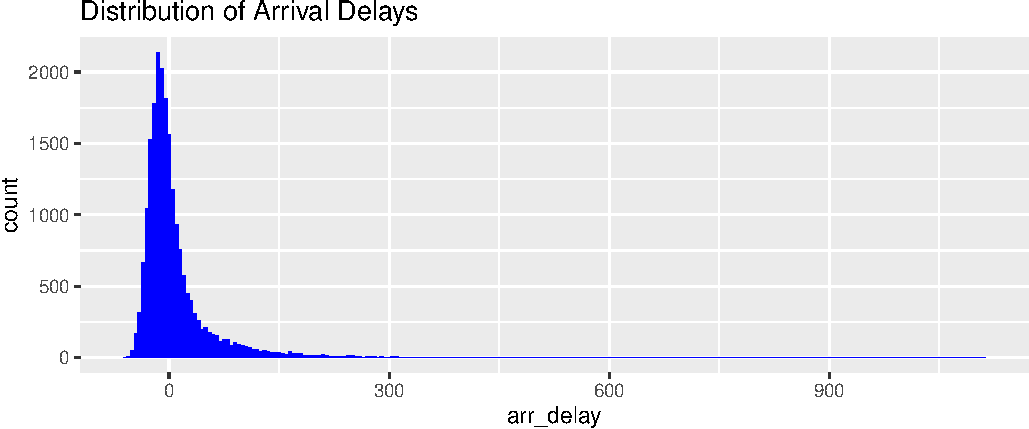
\includegraphics{Ch3_files/figure-pdf/unnamed-chunk-7-1.pdf}

We see that the distribution of arrival delays is heavily right-skewed.
While most flights arrive around the scheduled time, a few were late by
3 or more hours.

We'll calculate the mean arrival delay.

\begin{Shaded}
\begin{Highlighting}[]
\CommentTok{\#proportion of flights on time}
\NormalTok{mu }\OtherTok{\textless{}{-}} \FunctionTok{mean}\NormalTok{(Flights\_NY\_CHI}\SpecialCharTok{$}\NormalTok{arr\_delay)}
\NormalTok{mu}
\end{Highlighting}
\end{Shaded}

\begin{verbatim}
[1] 7.144772
\end{verbatim}

When the population parameter represents a mean, we'll denote it using
\(\mu\). Here \(\mu=\) 7.144772.

We also calculate the standard deviation of arrival delays.

\begin{Shaded}
\begin{Highlighting}[]
\CommentTok{\# mean arrival delay in sample}
\NormalTok{SD\_delay }\OtherTok{\textless{}{-}} \FunctionTok{sd}\NormalTok{(S1}\SpecialCharTok{$}\NormalTok{arr\_delay)}
\NormalTok{SD\_delay}
\end{Highlighting}
\end{Shaded}

\begin{verbatim}
[1] 60.10419
\end{verbatim}

\subsection{Sampling Variability}\label{sampling-variability}

We typically won't have data on the full population and won't know the
values of parameters like \(p\) and \(\mu\). Instead, we'll have data on
just a sample taken from the population.

To illustrate, we'll take a sample of 75 flights. The first 6 flights in
the sample are shown below. The \texttt{ontime} variable tells whether
or not the flight arrived on time.

\begin{Shaded}
\begin{Highlighting}[]
\CommentTok{\# take sample of 75 flights}
\FunctionTok{set.seed}\NormalTok{(}\DecValTok{08082023}\NormalTok{)}
\NormalTok{S1 }\OtherTok{\textless{}{-}} \FunctionTok{sample\_n}\NormalTok{(Flights\_NY\_CHI, }\DecValTok{75}\NormalTok{)}
\FunctionTok{head}\NormalTok{(S1)}
\end{Highlighting}
\end{Shaded}

\begin{verbatim}
# A tibble: 6 x 9
   year month   day carrier origin dest  sched_dep_time arr_delay ontime
  <int> <int> <int> <chr>   <chr>  <chr>          <int>     <dbl> <chr> 
1  2013     3     8 AA      LGA    ORD             1720       106 N     
2  2013    12    15 AA      JFK    ORD             1715       -24 Y     
3  2013    10    22 UA      EWR    ORD             1300       -12 Y     
4  2013     8    26 UA      EWR    ORD             2110        15 N     
5  2013     7    23 AA      LGA    ORD             1359        66 N     
6  2013     5    13 UA      EWR    ORD              900       -21 Y     
\end{verbatim}

We'll calculate the number, and proportion of flights that arrived on
time.

\begin{Shaded}
\begin{Highlighting}[]
\NormalTok{num\_ontime }\OtherTok{\textless{}{-}} \FunctionTok{sum}\NormalTok{(S1}\SpecialCharTok{$}\NormalTok{ontime }\SpecialCharTok{==} \StringTok{"Y"}\NormalTok{) }\CommentTok{\# count number of on{-}time arrivals}
\NormalTok{num\_ontime}
\end{Highlighting}
\end{Shaded}

\begin{verbatim}
[1] 39
\end{verbatim}

Proportion of on-time arrivals in the sample.

\begin{Shaded}
\begin{Highlighting}[]
\CommentTok{\# proportion of on{-}time flights in sample}
\NormalTok{p\_hat }\OtherTok{\textless{}{-}}\NormalTok{ num\_ontime}\SpecialCharTok{/}\DecValTok{75}
\NormalTok{p\_hat}
\end{Highlighting}
\end{Shaded}

\begin{verbatim}
[1] 0.52
\end{verbatim}

When the sample statistic is a proportion, it is commonly denoted
\(\hat{p}\).

In our sample \(\hat{p}\) = 52 percent of flights arrived on-time. The
sample statistic \(\hat{p}\) is an estimate of the population proportion
\(p\), the proportion of all flights arriving on time.

We also calculate the mean arrival delay in minutes.

\begin{Shaded}
\begin{Highlighting}[]
\CommentTok{\# mean arrival delay in sample}
\NormalTok{y\_bar }\OtherTok{\textless{}{-}} \FunctionTok{mean}\NormalTok{(S1}\SpecialCharTok{$}\NormalTok{arr\_delay)}
\NormalTok{y\_bar}
\end{Highlighting}
\end{Shaded}

\begin{verbatim}
[1] 19.2
\end{verbatim}

We'll denote this sample mean \(\bar{y}\). It is an estimate of the
population mean, representing the arrival mean delay for all flights,
which we'll denote \(\mu\).

Of course, this was just one sample of 75 flights. If we took different
samples of 75 flights, we would expect the statistics \(\hat{p}\) and
\(\bar{x}\) to vary from sample to sample.

Here's a different sample of 75 flights.

\begin{Shaded}
\begin{Highlighting}[]
\NormalTok{S2 }\OtherTok{\textless{}{-}} \FunctionTok{sample\_n}\NormalTok{(Flights\_NY\_CHI, }\DecValTok{75}\NormalTok{)}
\end{Highlighting}
\end{Shaded}

Proportion arriving on time in second sample:

\begin{Shaded}
\begin{Highlighting}[]
\CommentTok{\# proportion arriving on time in second sample}
\NormalTok{num\_ontime2 }\OtherTok{\textless{}{-}} \FunctionTok{sum}\NormalTok{(S2}\SpecialCharTok{$}\NormalTok{ontime }\SpecialCharTok{==} \StringTok{"Y"}\NormalTok{) }\CommentTok{\# count number of on{-}time arrivals}
\NormalTok{p\_hat2 }\OtherTok{\textless{}{-}}\NormalTok{ num\_ontime2}\SpecialCharTok{/}\DecValTok{75}
\NormalTok{p\_hat2}
\end{Highlighting}
\end{Shaded}

\begin{verbatim}
[1] 0.5066667
\end{verbatim}

Mean arrival delay in second sample:

\begin{Shaded}
\begin{Highlighting}[]
\CommentTok{\# mean arrival delay in second sample}
\NormalTok{y\_bar2 }\OtherTok{\textless{}{-}} \FunctionTok{mean}\NormalTok{(S2}\SpecialCharTok{$}\NormalTok{arr\_delay)}
\NormalTok{y\_bar2}
\end{Highlighting}
\end{Shaded}

\begin{verbatim}
[1] 15.28
\end{verbatim}

Sample statistics will vary from sample to sample, thus it is not
realistic to expect them to exactly match their corresponding population
parameters.

Nevertheless we can use the sample to estimate the proportion of all
flights in the population that arrive on time.

Let's take 10,000 more random samples of 75 flights and record the
proportion of on-time arrivals in each sample.

\begin{Shaded}
\begin{Highlighting}[]
\NormalTok{nreps }\OtherTok{\textless{}{-}} \DecValTok{10000}  \CommentTok{\# number of repetitions}
\NormalTok{p\_hat\_val }\OtherTok{\textless{}{-}} \FunctionTok{rep}\NormalTok{(}\ConstantTok{NA}\NormalTok{, nreps) }\CommentTok{\# create vector to hold proportion of on{-}time arrivals}
\NormalTok{y\_bar\_val }\OtherTok{\textless{}{-}} \FunctionTok{rep}\NormalTok{(}\ConstantTok{NA}\NormalTok{, nreps) }\CommentTok{\# create vector to hold mean arrival delay}

\NormalTok{Sample }\OtherTok{\textless{}{-}} \DecValTok{1}\SpecialCharTok{:}\NormalTok{nreps}

\ControlFlowTok{for}\NormalTok{(i }\ControlFlowTok{in} \DecValTok{1}\SpecialCharTok{:}\NormalTok{nreps)\{}
\NormalTok{S }\OtherTok{\textless{}{-}} \FunctionTok{sample\_n}\NormalTok{(Flights\_NY\_CHI, }\DecValTok{75}\NormalTok{) }\CommentTok{\# take sample of 75}
\NormalTok{N\_ontime }\OtherTok{\textless{}{-}} \FunctionTok{sum}\NormalTok{(S}\SpecialCharTok{$}\NormalTok{ontime }\SpecialCharTok{==} \StringTok{"Y"}\NormalTok{) }\CommentTok{\# count number of on{-}time arrivals}
\NormalTok{p\_hat\_val[i] }\OtherTok{\textless{}{-}}\NormalTok{ N\_ontime}\SpecialCharTok{/}\DecValTok{75} \CommentTok{\# record proportion on{-}time}
\NormalTok{y\_bar\_val[i] }\OtherTok{\textless{}{-}} \FunctionTok{mean}\NormalTok{(S}\SpecialCharTok{$}\NormalTok{arr\_delay) }\CommentTok{\# record mean arrival delay}
\NormalTok{\}}

\NormalTok{Samples\_df }\OtherTok{\textless{}{-}} \FunctionTok{data.frame}\NormalTok{(Sample, p\_hat\_val, y\_bar\_val) }\CommentTok{\# store results in a data frame}
\end{Highlighting}
\end{Shaded}

The table shows the proportion of on-time arrivals in the first 20
samples of 75 flights.

\begin{Shaded}
\begin{Highlighting}[]
\FunctionTok{kable}\NormalTok{(}\FunctionTok{head}\NormalTok{(Samples\_df, }\DecValTok{20}\NormalTok{) }\SpecialCharTok{|\textgreater{}} \FunctionTok{round}\NormalTok{(}\DecValTok{2}\NormalTok{))}
\end{Highlighting}
\end{Shaded}

\begin{longtable}[]{@{}rrr@{}}
\toprule\noalign{}
Sample & p\_hat\_val & y\_bar\_val \\
\midrule\noalign{}
\endhead
\bottomrule\noalign{}
\endlastfoot
1 & 0.65 & 6.16 \\
2 & 0.53 & 10.75 \\
3 & 0.59 & 12.41 \\
4 & 0.69 & 2.24 \\
5 & 0.59 & 7.33 \\
6 & 0.67 & 1.28 \\
7 & 0.61 & 3.25 \\
8 & 0.59 & 8.93 \\
9 & 0.65 & -3.16 \\
10 & 0.65 & 5.73 \\
11 & 0.61 & 12.32 \\
12 & 0.59 & 8.79 \\
13 & 0.61 & 5.53 \\
14 & 0.48 & 10.55 \\
15 & 0.60 & 5.40 \\
16 & 0.44 & 24.11 \\
17 & 0.49 & 15.93 \\
18 & 0.57 & 4.45 \\
19 & 0.64 & 6.76 \\
20 & 0.56 & 3.65 \\
\end{longtable}

The histogram below shows the distribution of the proportion of on-time
arrivals in the 10,000 different samples.

\begin{Shaded}
\begin{Highlighting}[]
\NormalTok{Prop\_Samp\_Dist}\OtherTok{\textless{}{-}} \FunctionTok{ggplot}\NormalTok{(}\AttributeTok{data=}\NormalTok{Samples\_df, }\FunctionTok{aes}\NormalTok{(}\AttributeTok{x=}\NormalTok{p\_hat\_val)) }\SpecialCharTok{+}
  \FunctionTok{geom\_histogram}\NormalTok{(}\AttributeTok{color=}\StringTok{"blue"}\NormalTok{, }\AttributeTok{fill=}\StringTok{"blue"}\NormalTok{, }\AttributeTok{binwidth=}\FloatTok{0.001}\NormalTok{) }\SpecialCharTok{+} 
  \FunctionTok{ggtitle}\NormalTok{(}\StringTok{"Sampling Distribution for Proportion On Time"}\NormalTok{) }\SpecialCharTok{+} 
  \FunctionTok{xlab}\NormalTok{(}\StringTok{"Prop. on time in sample"}\NormalTok{)}
\NormalTok{Prop\_Samp\_Dist}
\end{Highlighting}
\end{Shaded}

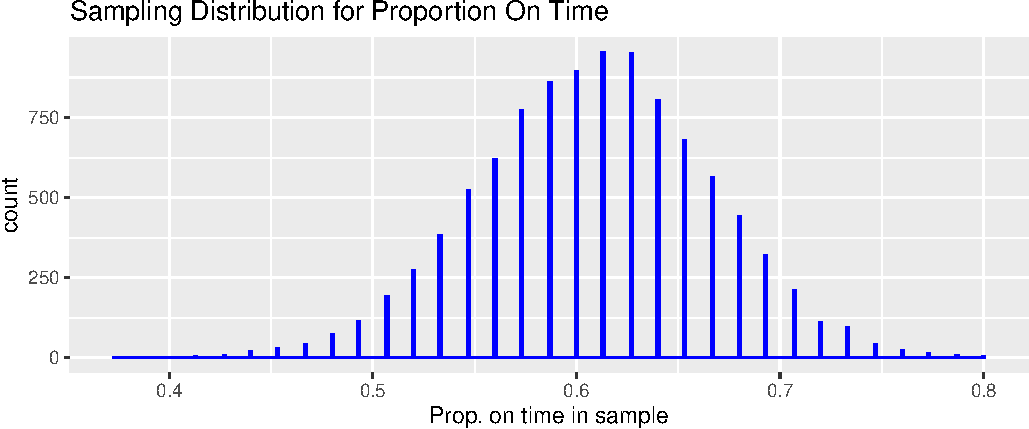
\includegraphics{Ch3_files/figure-pdf/unnamed-chunk-19-1.pdf}

We notice that most of our 10,000 samples yielded proportions of on-time
arrivals between 0.5 and 0.7, The distribution of proportion of on-time
arrivals is roughly symmetric and bell-shaped.

The distribution shown in this histogram is called the \textbf{sampling
distribution for} \(\hat{p}\). The sampling distribution for a statistic
shows the distribution of the statistic over many samples.

We'll calculate the mean of the sampling distribution for \(\hat{p}\).
How does it compare to the true population parameter \(p\)?

\begin{Shaded}
\begin{Highlighting}[]
\NormalTok{Mean\_p\_hat }\OtherTok{\textless{}{-}} \FunctionTok{mean}\NormalTok{(Samples\_df}\SpecialCharTok{$}\NormalTok{p\_hat\_val)}
\NormalTok{Mean\_p\_hat}
\end{Highlighting}
\end{Shaded}

\begin{verbatim}
[1] 0.60848
\end{verbatim}

We can gauge how much the proportion of on-time arrivals varies between
samples by calculating the standard deviation of this sampling
distribution. The standard deviation of a sampling distribution for a
statistic is also called the \textbf{standard error} of the statistic.
In this case it represents the standard error \(\hat{p}\) (the
proportion of on-time arrivals), and is denoted \(\text{SE}(\hat{p})\).
This standard error is shown below.

\begin{Shaded}
\begin{Highlighting}[]
\NormalTok{SE\_p\_hat }\OtherTok{\textless{}{-}} \FunctionTok{sd}\NormalTok{(Samples\_df}\SpecialCharTok{$}\NormalTok{p\_hat\_val)}
\NormalTok{SE\_p\_hat}
\end{Highlighting}
\end{Shaded}

\begin{verbatim}
[1] 0.05659102
\end{verbatim}

Now, we'll examine the sampling distribution of the mean arrival time
\(\bar{y}\).

\begin{Shaded}
\begin{Highlighting}[]
\NormalTok{Mean\_Samp\_Dist}\OtherTok{\textless{}{-}} \FunctionTok{ggplot}\NormalTok{(}\AttributeTok{data=}\NormalTok{Samples\_df, }\FunctionTok{aes}\NormalTok{(}\AttributeTok{x=}\NormalTok{y\_bar\_val)) }\SpecialCharTok{+}
  \FunctionTok{geom\_histogram}\NormalTok{(}\AttributeTok{color=}\StringTok{"white"}\NormalTok{, }\AttributeTok{fill=}\StringTok{"blue"}\NormalTok{, }\AttributeTok{binwidth=}\FloatTok{0.5}\NormalTok{) }\SpecialCharTok{+} 
  \FunctionTok{ggtitle}\NormalTok{(}\StringTok{"Sampling Distribution for Mean Arrival Delay"}\NormalTok{) }\SpecialCharTok{+} 
  \FunctionTok{xlab}\NormalTok{(}\StringTok{"Mean Arrival Delay"}\NormalTok{)}
\NormalTok{Mean\_Samp\_Dist}
\end{Highlighting}
\end{Shaded}

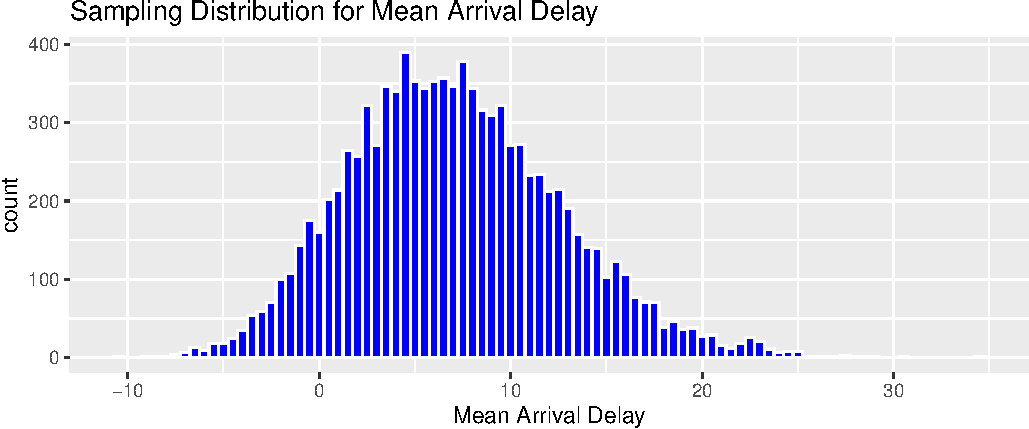
\includegraphics{Ch3_files/figure-pdf/unnamed-chunk-22-1.pdf}

How does the sampling distribution for mean arrival delays compare to
the distribution of arrival delays for individual flights? Think about
the shape and the variability of the distributions.

\begin{Shaded}
\begin{Highlighting}[]
\NormalTok{mean\_y\_bar }\OtherTok{\textless{}{-}} \FunctionTok{mean}\NormalTok{(Samples\_df}\SpecialCharTok{$}\NormalTok{y\_bar\_val)}
\FunctionTok{mean}\NormalTok{(mean\_y\_bar)}
\end{Highlighting}
\end{Shaded}

\begin{verbatim}
[1] 7.081397
\end{verbatim}

The standard error of the mean, \(SE(\bar{y})\) is shown calculated
below.

\begin{Shaded}
\begin{Highlighting}[]
\NormalTok{SE\_y\_bar }\OtherTok{\textless{}{-}} \FunctionTok{sd}\NormalTok{(Samples\_df}\SpecialCharTok{$}\NormalTok{y\_bar\_val)}
\NormalTok{SE\_y\_bar}
\end{Highlighting}
\end{Shaded}

\begin{verbatim}
[1] 5.563925
\end{verbatim}

What does this standard error represent? How is it different than the
the standard deviation of flight times, which we previously saw was 60.1
minutes?

\textbf{Vocabulary:}

\begin{itemize}
\tightlist
\item
  The \textbf{sampling distribution} of a statistic is the distribution
  of values the statistic takes on across many different samples of a
  given size.\\
\item
  The \textbf{standard error} of a statistic is the standard deviation
  of that statistic's sampling distribution. It measures how much the
  statistic varies between different samples of a given size.
\end{itemize}

\subsection{Sample Size and Standard
Error}\label{sample-size-and-standard-error}

\textbf{Question:}

Suppose the sample consisted of 10, or 30, or 500 flights, instead of
75? Would you expect the standard deviation of individual flight times
to increase, decrease or stay about the same? What about the standard
error of the mean delay?

The histogram shows the distribution of individual flight delays in
random samples of each size.

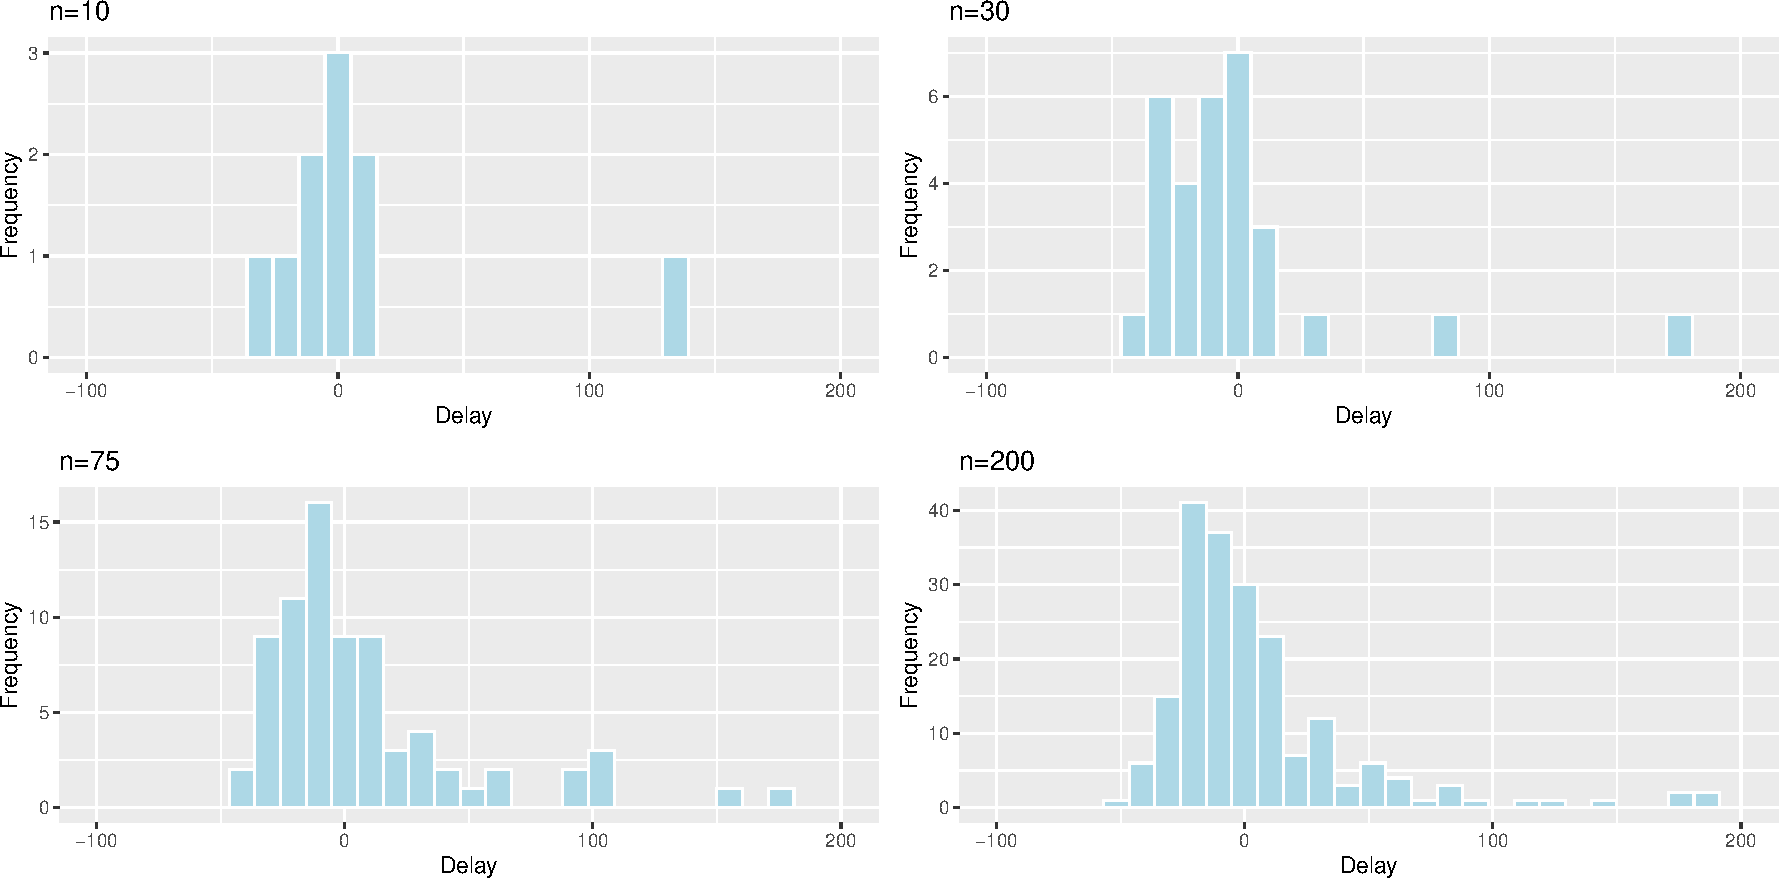
\includegraphics{Ch3_files/figure-pdf/unnamed-chunk-26-1.pdf}

For each sample, most of the flights have delays slightly below or above
0, though a small percentage of the flights in each sample have much
larger delays. The variability in delays is about the same, regardless
of sample size.

The table shows the standard deviation in each of the samples.

\begin{longtable}[]{@{}rr@{}}
\toprule\noalign{}
Sample\_Size & SD \\
\midrule\noalign{}
\endhead
\bottomrule\noalign{}
\endlastfoot
10 & 45.38673 \\
30 & 40.64390 \\
75 & 43.40787 \\
200 & 48.01117 \\
\end{longtable}

Sample size does not impact the amount of variability between individual
flights. Standard deviation in delay times does not systematically
increase or decrease based on sample size (of course it varies a little
based on the lakes randomly chosen in the sample).

Now, we'll examine what happens to the standard error of the mean as the
sample size changes.

\textbf{Distributions of Mean Between Different Samples}

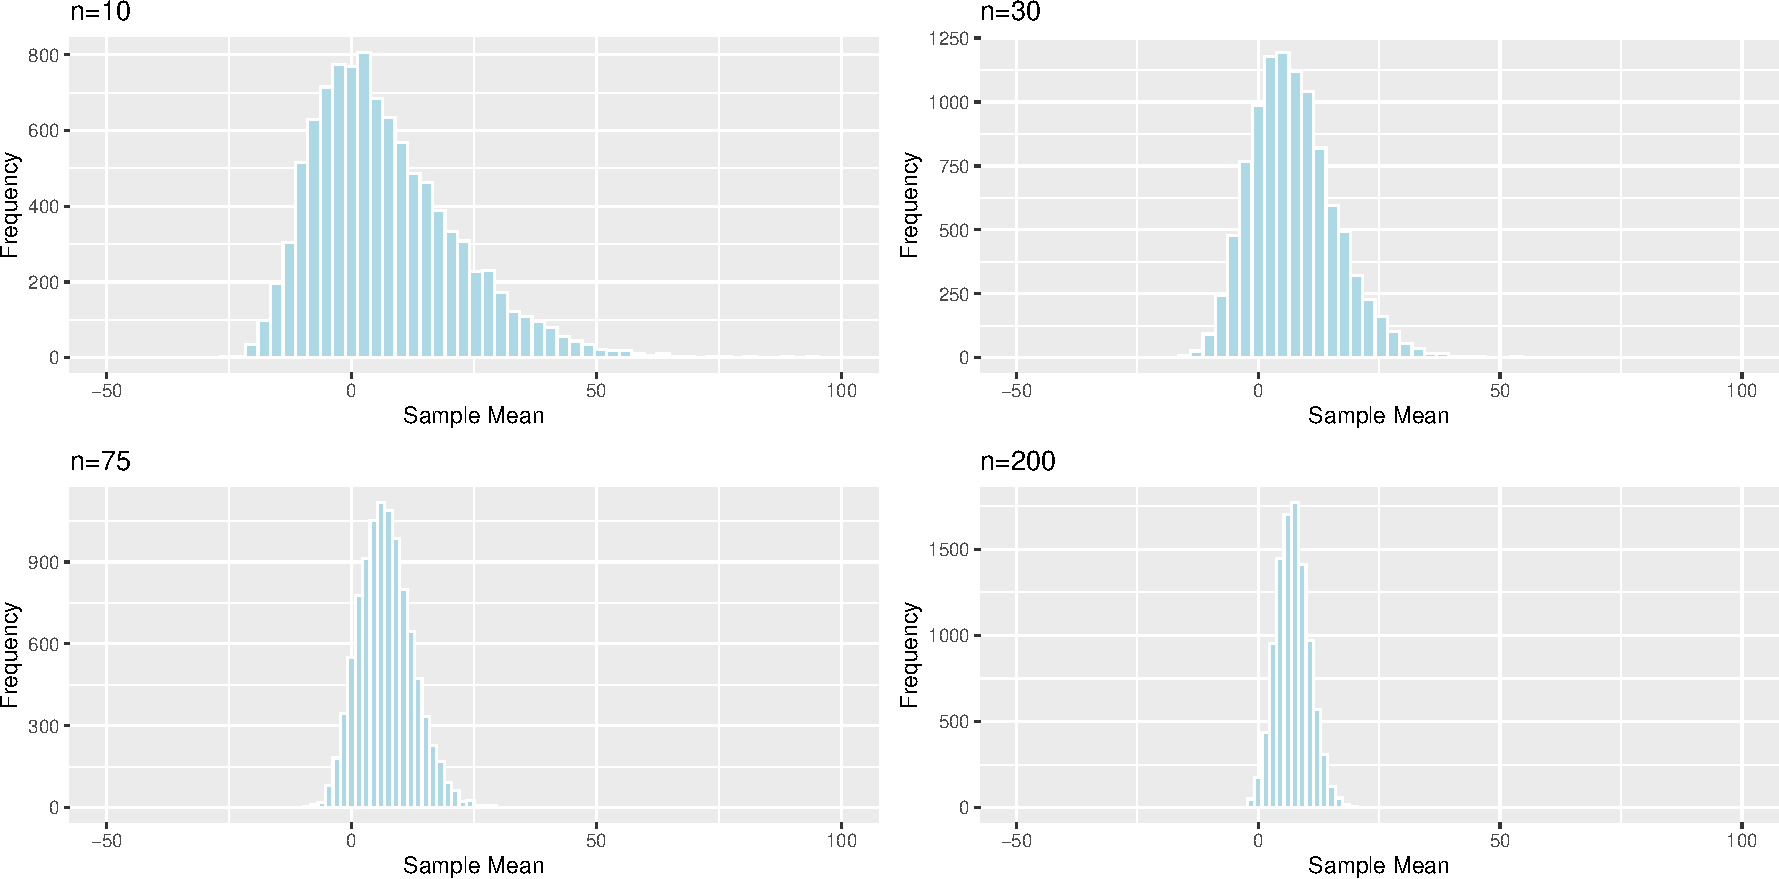
\includegraphics{Ch3_files/figure-pdf/unnamed-chunk-29-1.pdf}

Notice that as the sample size increases, the sampling distribution of
the mean becomes more symmetric and bell-shaped, and also more
concentrated around the population mean \(\mu\).

The table shows the standard error of the mean for samples of different
size:

\begin{longtable}[]{@{}rr@{}}
\toprule\noalign{}
Sample\_Size & SE \\
\midrule\noalign{}
\endhead
\bottomrule\noalign{}
\endlastfoot
10 & 15.027787 \\
30 & 8.832375 \\
75 & 5.461011 \\
200 & 3.371757 \\
\end{longtable}

As sample size increases, variability between means of different samples
decreases. Standard error of the mean decreases. This is also true of
standard errors for other statistics (i.e.~difference in means,
regression slopes, etc.)

\section{Confidence Intervals}\label{confidence-intervals}

\subsection{Constructing Confidence
Intervals}\label{constructing-confidence-intervals}

We saw that while statistics calculated from individual samples deviate
from population parameters, over many samples, they approximately
average to the population parameter (assuming the samples are chosen
randomly).

Thus, when we have only a single sample, we can use the sample statistic
as an estimate of the population parameter, provided we allow for a
certain margin of error. The question is how much margin of error do we
need?

The sampling distribution for the proportion of on-time flights is shown
again below. The true proportion of on-time flights (\(p=0.607984\)) is
marked by the green dotted line. The gold bar at the bottom of the
histogram represents the range of sample proportions that lie within
\(\pm 2\) standard errors of the true population proportion of flights
that arrived on time:

0.608 - 2(0.057) = 0.495 to 0.608 + 2(0.057) = 0.721

\begin{Shaded}
\begin{Highlighting}[]
\NormalTok{Prop\_Samp\_Dist }\SpecialCharTok{+} \FunctionTok{geom\_vline}\NormalTok{(}\AttributeTok{xintercept=}\NormalTok{p, }\AttributeTok{color=}\StringTok{"green"}\NormalTok{, }\AttributeTok{linetype=}\StringTok{"dotted"}\NormalTok{, }\AttributeTok{linewidth=}\DecValTok{2}\NormalTok{) }\SpecialCharTok{+} \FunctionTok{geom\_segment}\NormalTok{(}\FunctionTok{aes}\NormalTok{(}\AttributeTok{x=}\NormalTok{p }\SpecialCharTok{{-}} \DecValTok{2}\SpecialCharTok{*}\NormalTok{SE\_p\_hat,}\AttributeTok{xend=}\NormalTok{p }\SpecialCharTok{+} \DecValTok{2}\SpecialCharTok{*}\NormalTok{SE\_p\_hat, }\AttributeTok{y=}\DecValTok{50}\NormalTok{, }\AttributeTok{yend=}\DecValTok{50}\NormalTok{), }\AttributeTok{color=}\StringTok{"gold"}\NormalTok{, }\AttributeTok{size=}\DecValTok{10}\NormalTok{, }\AttributeTok{alpha=}\FloatTok{0.01}\NormalTok{) }
\end{Highlighting}
\end{Shaded}

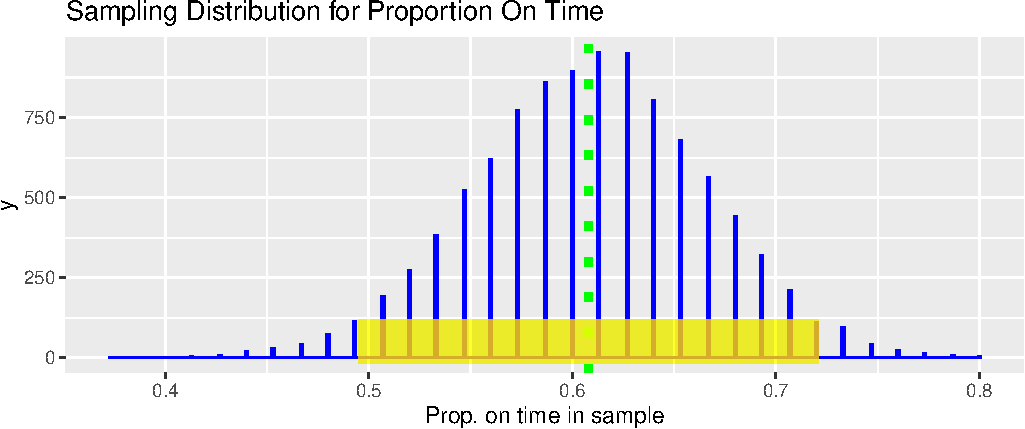
\includegraphics{Ch3_files/figure-pdf/unnamed-chunk-31-1.pdf}

We calculate the proportion of samples whose proportion of on-time
arrivals lies within \(\pm 2\) standard errors of the true proportion.

\begin{Shaded}
\begin{Highlighting}[]
\NormalTok{Lower }\OtherTok{\textless{}{-}}\NormalTok{ p }\SpecialCharTok{{-}} \DecValTok{2}\SpecialCharTok{*}\NormalTok{SE\_p\_hat}
\NormalTok{Upper }\OtherTok{\textless{}{-}}\NormalTok{ p }\SpecialCharTok{+} \DecValTok{2}\SpecialCharTok{*}\NormalTok{SE\_p\_hat}
\FunctionTok{sum}\NormalTok{((Samples\_df}\SpecialCharTok{$}\NormalTok{p\_hat\_val }\SpecialCharTok{\textgreater{}=}\NormalTok{Lower) }\SpecialCharTok{\&}\NormalTok{ (Samples\_df}\SpecialCharTok{$}\NormalTok{p\_hat\_val }\SpecialCharTok{\textless{}=}\NormalTok{ Upper))}
\end{Highlighting}
\end{Shaded}

\begin{verbatim}
[1] 9539
\end{verbatim}

Approximately 95\% 10,000 samples produced proportions within \(\pm 2\)
standard errors of the true population proportion of on-time flights.

In a real situation, we won't have access to the entire population of
flights, only the flights in a single sample. For example, recall our
original sample of 75 flights, in which we observed a proportion of
on-time arrivals of \(\hat{p}=\) 0.52.

Since we now know that 95\% of all samples produce proportions that lie
within two standard errors of the population proportion, we can obtain
an estimate of the population proportion \(p\) by adding and subtracting
\(2\times \text{SE}(\hat{p})\) from our observed sample proportion
\(\hat{p}\).

Using probability theory, it can be shown generally that if the sampling
distribution of a statistic is symmetric and bell shaped, then
approximately 95\% of all samples will produce sample statistics that
lie within two standard errors of the corresponding population
parameter. Such an interval is called an approximate 95\%
\textbf{confidence interval} for the population parameter.

\textbf{Approximate 95\% confidence interval: If the sampling
distribution of a statistic is symmetric and bell-shaped, a 95\%
confidence interval for the population parameter is:}

\[
\text{Statistic} \pm 2\times \text{Standard Error}, 
\]

More generally, if we want to use a level of confidence that is
different than 95\%, we can adjust the value we multiply the standard
error by. In general, a standard error confidence interval has the form:

\[
\text{Statistic } \pm m\times \text{Standard Error}, 
\]

where the value of \(m\) depends on the desired level of confidence.

Confidence intervals that are calculated by adding and subtracting a
certain number of standard errors from the sample statistic are called
\textbf{standard error confidence intervals}. This approach works as
long as the sampling distribution is symmetric and bell-shaped.
Probability theory tells us that in a symmetric and bell-shaped
distribution, approximately 95\% of the area lies within two standard
errors of the center of the distribution, given by the true parameter
value. We will, however, see that this approach will not work in all
cases. Not all statistics produce sampling distributions that are
symmetric and bell-shaped, and we will need an alternative way to
calculate confidence intervals in these situations.

\begin{figure}[H]

{\centering 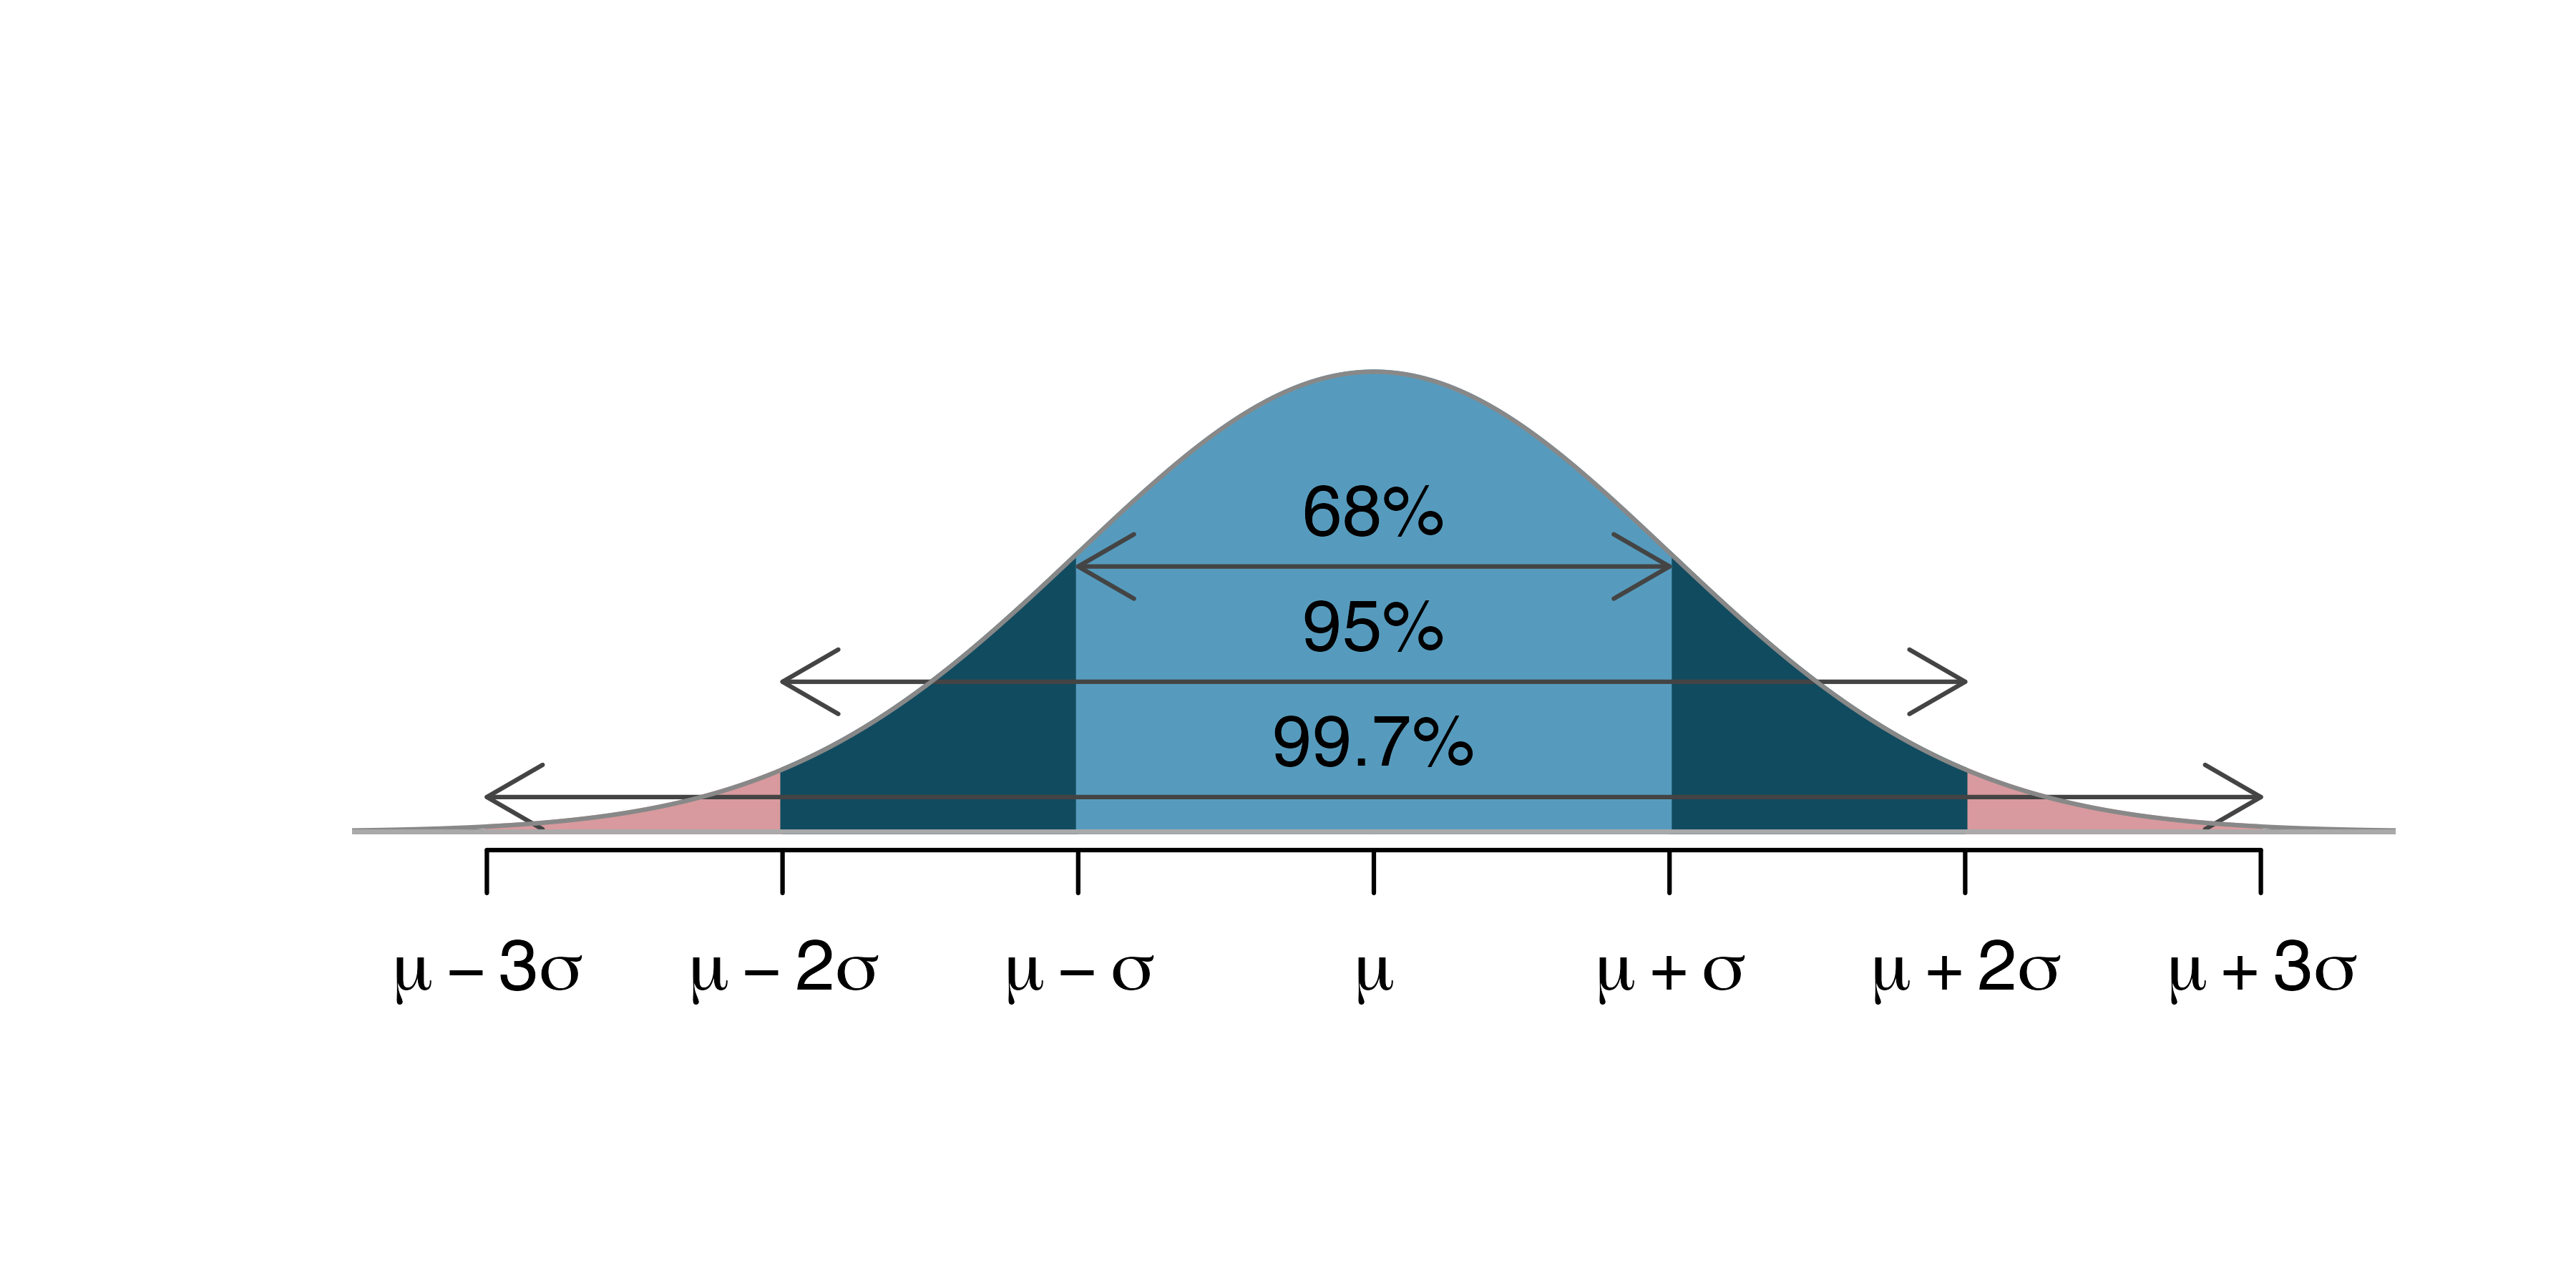
\includegraphics{Emp_Rule.png}

}

\caption{Image from
https://openintro-ims.netlify.app/foundations-mathematical}

\end{figure}%

\subsubsection{\texorpdfstring{Example: 95\% Confidence Interval for
\(p\)}{Example: 95\% Confidence Interval for p}}\label{example-95-confidence-interval-for-p}

We'll calculate a 95\% confidence interval for the proportion of on-time
flights, using our original sample where \(\hat{p}\) = 0.52. The 95\%
confidence interval is:

\[
\begin{aligned}
& \hat{p} \pm 2\times \text{SE}(\hat{p}) \\
& = 0.52 \pm 2(0.056591)
\end{aligned}
\]

The confidence interval is calculated below.

\begin{Shaded}
\begin{Highlighting}[]
\FunctionTok{c}\NormalTok{(p\_hat }\SpecialCharTok{{-}} \DecValTok{2}\SpecialCharTok{*}\NormalTok{SE\_p\_hat, p\_hat }\SpecialCharTok{+} \DecValTok{2}\SpecialCharTok{*}\NormalTok{SE\_p\_hat) }
\end{Highlighting}
\end{Shaded}

\begin{verbatim}
[1] 0.406818 0.633182
\end{verbatim}

Based on our sample of 75 flights, we can be 95\% confident that the
true proportion of on-time arrivals among all 2013 flights from New York
to Chicago is between 0.407 and 0.633.

\subsubsection{\texorpdfstring{Example: 95\% Confidence Interval for
\(\mu\)}{Example: 95\% Confidence Interval for \textbackslash mu}}\label{example-95-confidence-interval-for-mu}

Likewise, we calculate a 95\% confidence interval for average arrival
delay using the formula:

\[
\begin{aligned}
\bar{y} \pm 2\times \text{SE}(\bar{y}) \\
& = 19.2 \pm 2(5.5639246)
\end{aligned}
\]

\begin{Shaded}
\begin{Highlighting}[]
\FunctionTok{c}\NormalTok{(y\_bar }\SpecialCharTok{{-}} \DecValTok{2}\SpecialCharTok{*}\NormalTok{SE\_y\_bar, y\_bar }\SpecialCharTok{+} \DecValTok{2}\SpecialCharTok{*}\NormalTok{SE\_y\_bar) }
\end{Highlighting}
\end{Shaded}

\begin{verbatim}
[1]  8.072151 30.327849
\end{verbatim}

Based on our sample of 75 flights, we can be 95\% confident that the
mean arrival delay among all 2013 flights from New York to Chicago is
between 8.1 and 30.3 minutes.

Note that this is a statement about what we think is true of the mean
overall flight time, not the time of an individual flight. It would be
incorrect to say that we are 95\% confident that an individual flight
would be expected to have a delay in this interval. You might think
about whether the interval for the delay time of an individual flight
should be wider or narrower than this. We'll talk about such an interval
later in the term.

\subsection{What does 95\% Confidence
Mean?}\label{what-does-95-confidence-mean}

Knowing what we do about the true value of the population parameters
\(p\) and \(\mu\), we can see that our interval for \(p\), which was
(0.407, 0.633) does indeed contain the true population value of \(p=\)
0.6079841. However, the interval for \(\mu\), which was (8.1, 30.3) does
not contain the true value of \(\mu=\) 7.144772.

Does this mean we did something wrong when we calculated the interval
for \(\mu\), the average flight delay among all flights in the
population? The answer is ``no''. Notice we claimed to be only ``95\%''
confident that our interval contains the true value of the population
parameter \(\mu\). This means that we should expect 5\% of samples taken
randomly to yield a sample mean \(\bar{y}\) so different from the
population mean \(\mu\), that the resulting confidence interval would
not contain the true value of \(\mu\). This does not mean we did
anything wrong, just that we obtained an unusual sample just by chance.
Since our procedure, namely adding and subtracting two standard errors,
is designed to work 95\% of the time, we can expect such samples to be
rare.

In a real situation, we won't know the true value of the population
parameter, so we won't know for sure whether or not our confidence
interval contains this true parameter value.

To further understand the meaning of ``95\% confidence'', let's explore
what happens when we calculate confidence intervals based on estimates
\(\bar{y}\) obtained from many different samples. For each of our 10,000
different samples taken from our population, we'll add and subtract two
standard errors from the sample proportion \(\hat{p}\) corresponding to
that sample.

The table below displays the value of \(\hat{p}\), for the first 20
samples we took, along with the lower and upper bounds of the confidence
interval, and whether or not the confidence interval contains the true
parameter value \(p\) (either 1=\texttt{TRUE} or 0=\texttt{FALSE}).

\begin{Shaded}
\begin{Highlighting}[]
\NormalTok{Samples\_df\_p }\OtherTok{\textless{}{-}}\NormalTok{ Samples\_df }\SpecialCharTok{\%\textgreater{}\%} \FunctionTok{mutate}\NormalTok{(}\AttributeTok{Lower =}\NormalTok{ p\_hat\_val }\SpecialCharTok{{-}} \DecValTok{2}\SpecialCharTok{*}\NormalTok{SE\_p\_hat, }
                                     \AttributeTok{Upper =}\NormalTok{ p\_hat\_val }\SpecialCharTok{+} \DecValTok{2}\SpecialCharTok{*}\NormalTok{SE\_p\_hat,}
                                     \AttributeTok{Containsp =}\NormalTok{ p }\SpecialCharTok{\textgreater{}=}\NormalTok{ Lower }\SpecialCharTok{\&}\NormalTok{ p }\SpecialCharTok{\textless{}=}\NormalTok{ Upper) }\SpecialCharTok{|\textgreater{}}
                              \FunctionTok{select}\NormalTok{(Sample, p\_hat\_val, Lower, Upper, Containsp)  }
\FunctionTok{kable}\NormalTok{(}\FunctionTok{head}\NormalTok{(Samples\_df\_p }\SpecialCharTok{|\textgreater{}} \FunctionTok{round}\NormalTok{(}\DecValTok{2}\NormalTok{), }\DecValTok{20}\NormalTok{))}
\end{Highlighting}
\end{Shaded}

\begin{longtable}[]{@{}rrrrr@{}}
\toprule\noalign{}
Sample & p\_hat\_val & Lower & Upper & Containsp \\
\midrule\noalign{}
\endhead
\bottomrule\noalign{}
\endlastfoot
1 & 0.65 & 0.54 & 0.77 & 1 \\
2 & 0.53 & 0.42 & 0.65 & 1 \\
3 & 0.59 & 0.47 & 0.70 & 1 \\
4 & 0.69 & 0.58 & 0.81 & 1 \\
5 & 0.59 & 0.47 & 0.70 & 1 \\
6 & 0.67 & 0.55 & 0.78 & 1 \\
7 & 0.61 & 0.50 & 0.73 & 1 \\
8 & 0.59 & 0.47 & 0.70 & 1 \\
9 & 0.65 & 0.54 & 0.77 & 1 \\
10 & 0.65 & 0.54 & 0.77 & 1 \\
11 & 0.61 & 0.50 & 0.73 & 1 \\
12 & 0.59 & 0.47 & 0.70 & 1 \\
13 & 0.61 & 0.50 & 0.73 & 1 \\
14 & 0.48 & 0.37 & 0.59 & 0 \\
15 & 0.60 & 0.49 & 0.71 & 1 \\
16 & 0.44 & 0.33 & 0.55 & 0 \\
17 & 0.49 & 0.38 & 0.61 & 0 \\
18 & 0.57 & 0.46 & 0.69 & 1 \\
19 & 0.64 & 0.53 & 0.75 & 1 \\
20 & 0.56 & 0.45 & 0.67 & 1 \\
\end{longtable}

The graphic below visualizes the confidence intervals produced using the
estimates from the first 100 samples. The green dotted line indicates
the true value of \(p\). The black dots indicate the value of
\(\hat{p}\) for each sample. Intervals that do in fact contain the true
value of \(p\) are shown in blue, and intervals that do not contain the
true value of \(p\) are shown in green.

\begin{Shaded}
\begin{Highlighting}[]
\FunctionTok{ggplot}\NormalTok{(}\AttributeTok{data=}\NormalTok{Samples\_df\_p[}\DecValTok{1}\SpecialCharTok{:}\DecValTok{100}\NormalTok{,], }\FunctionTok{aes}\NormalTok{(}\AttributeTok{y=}\NormalTok{Sample, }\AttributeTok{x=}\NormalTok{p\_hat\_val)) }\SpecialCharTok{+}    
  \FunctionTok{geom\_point}\NormalTok{() }\SpecialCharTok{+}
  \FunctionTok{geom\_errorbar}\NormalTok{(}\FunctionTok{aes}\NormalTok{(}\AttributeTok{xmin =}\NormalTok{ Lower, }\AttributeTok{xmax =}\NormalTok{ Upper, }\AttributeTok{color=}\NormalTok{Containsp))  }\SpecialCharTok{+} 
  \FunctionTok{xlab}\NormalTok{(}\StringTok{"Confidence Interval"}\NormalTok{) }\SpecialCharTok{+} 
  \FunctionTok{ylab}\NormalTok{(}\StringTok{"Sample"}\NormalTok{) }\SpecialCharTok{+} 
  \FunctionTok{geom\_vline}\NormalTok{(}\AttributeTok{xintercept =}\NormalTok{ p, }\AttributeTok{color=}\StringTok{"green"}\NormalTok{, }\AttributeTok{linetype=}\StringTok{"dotted"}\NormalTok{, }\AttributeTok{size=}\DecValTok{2}\NormalTok{) }\SpecialCharTok{+} 
  \FunctionTok{ggtitle}\NormalTok{(}\StringTok{"100 Different Confidence Intervals for p"}\NormalTok{) }\SpecialCharTok{+} 
  \FunctionTok{theme\_bw}\NormalTok{() }
\end{Highlighting}
\end{Shaded}

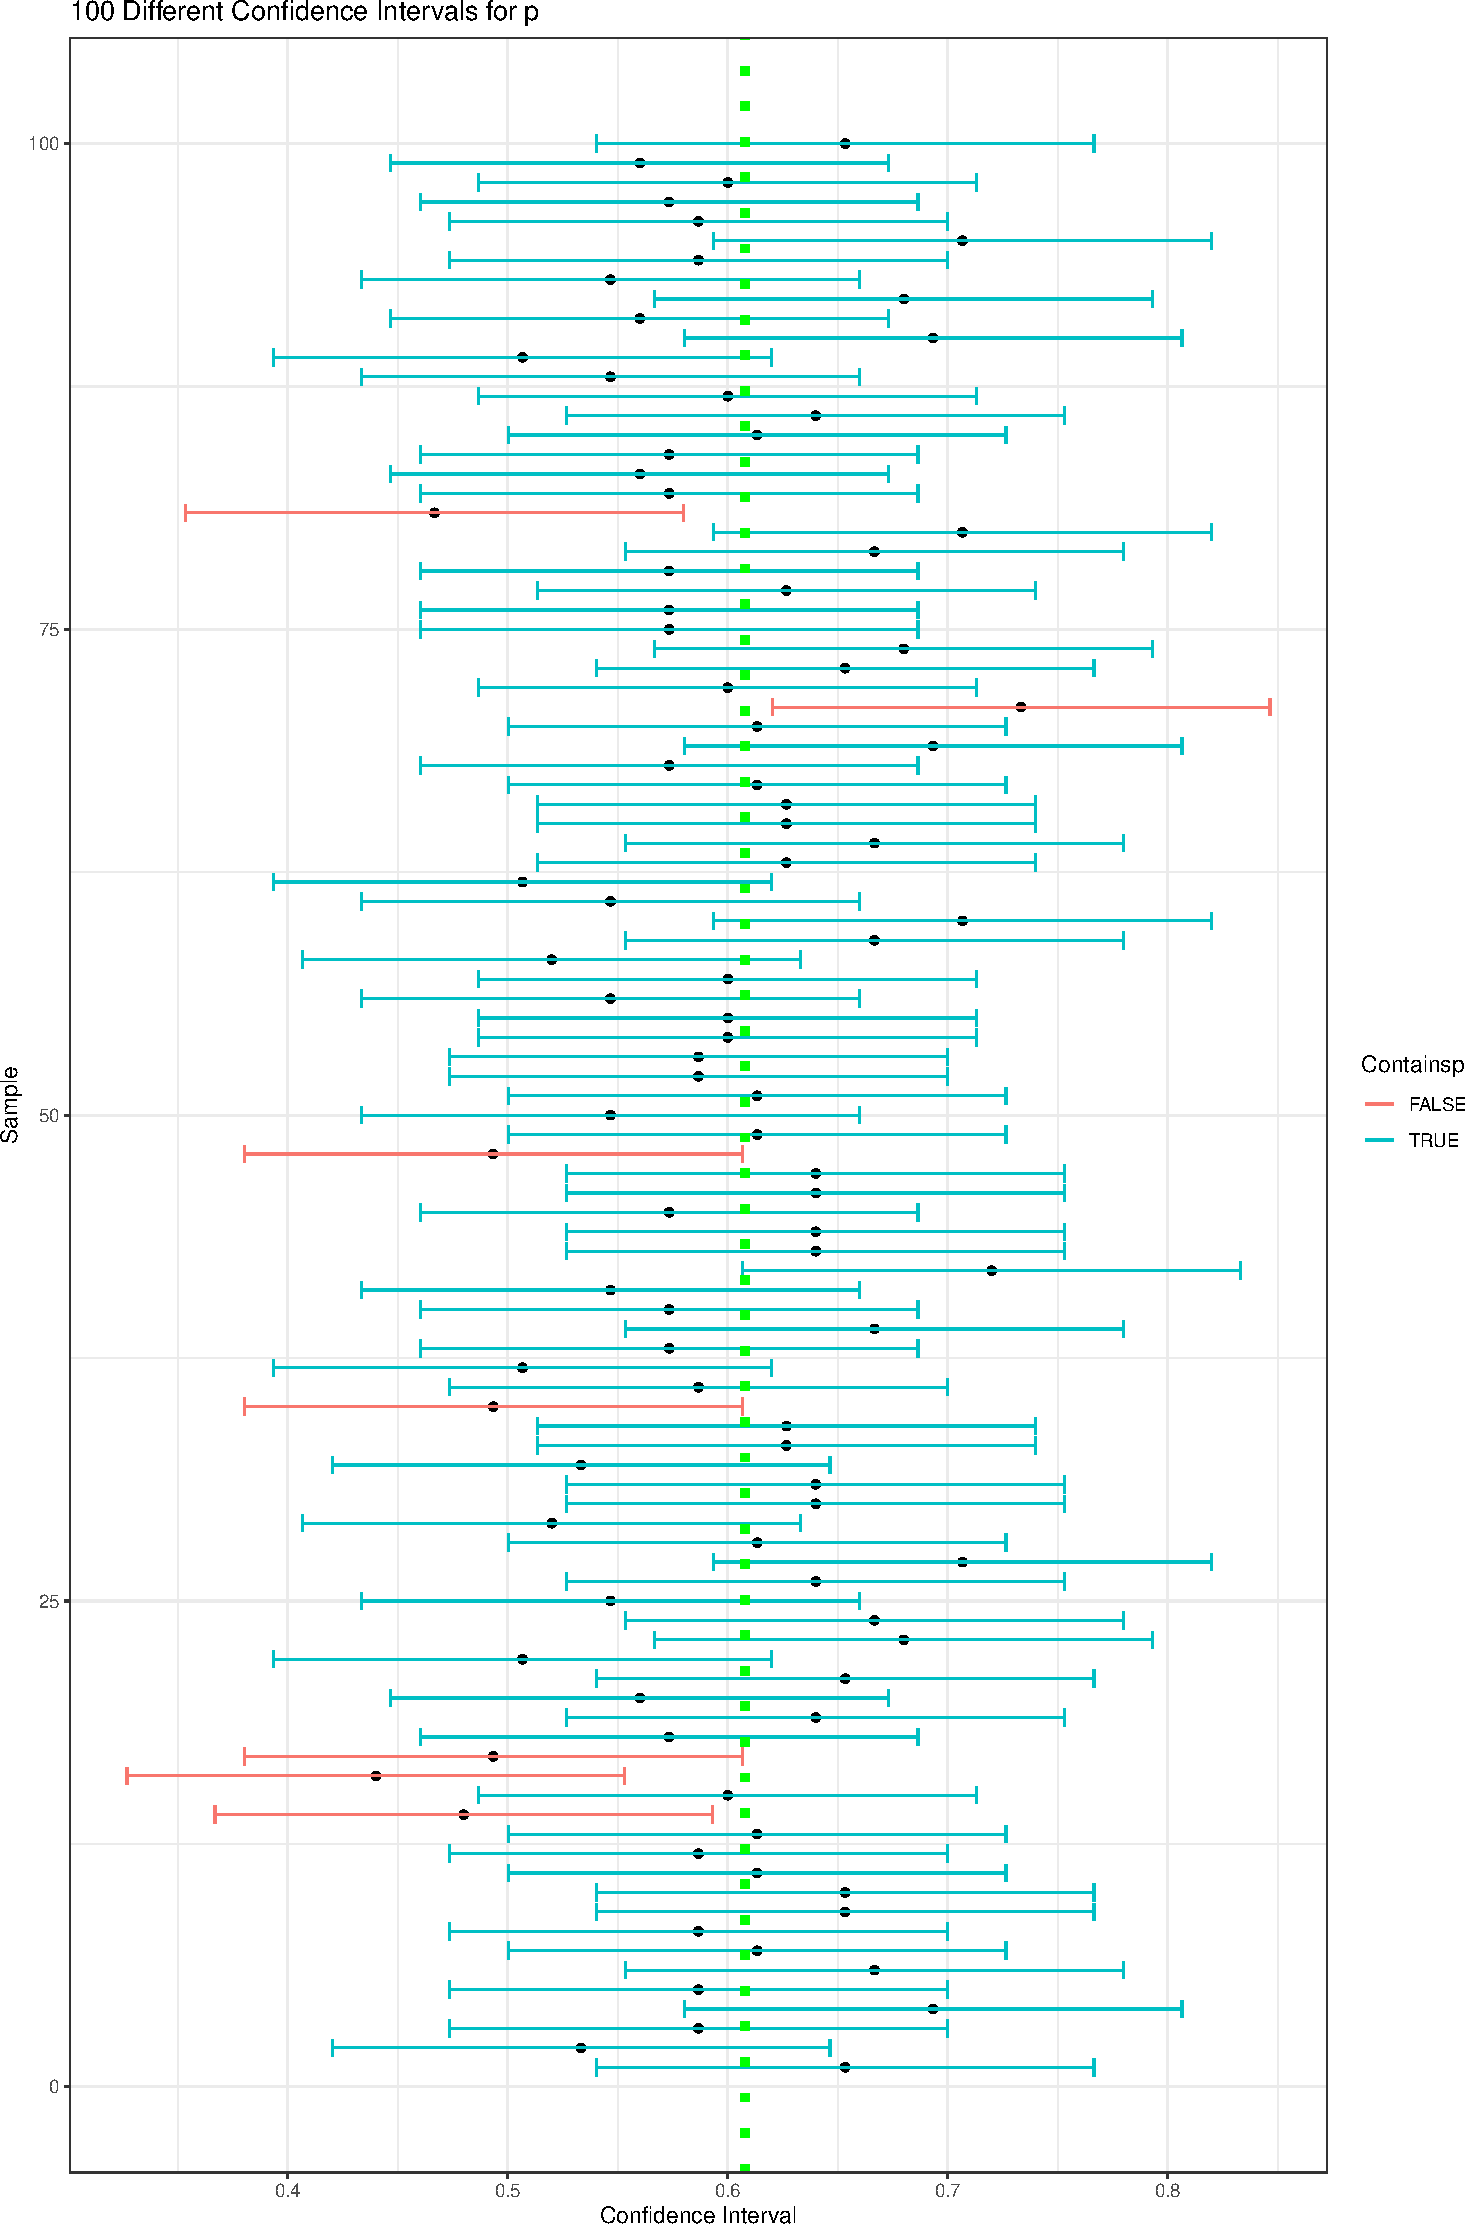
\includegraphics{Ch3_files/figure-pdf/unnamed-chunk-37-1.pdf}

Out of these 100 samples, 93 contain the true value of the population
parameter \(p\). This is close to the desired 95\% confidence level.

The picture shows confidence intervals produced by the first 100
samples, but we actually took 10,000 different samples of 75 flights.
Let's calculate how many of these samples produced confidence intervals
that contain the true value of \(p\).

\begin{Shaded}
\begin{Highlighting}[]
\FunctionTok{sum}\NormalTok{(Samples\_df\_p}\SpecialCharTok{$}\NormalTok{Contains }\SpecialCharTok{==} \ConstantTok{TRUE}\NormalTok{)}
\end{Highlighting}
\end{Shaded}

\begin{verbatim}
[1] 9539
\end{verbatim}

Again, notice that close to 95\% of the samples produced confidence
intervals contain the true population parameter \(p\). Note that for the
red intervals that do not contain \(p\) nothing was done incorrectly.
The sample was taken at random, and the confidence interval was
calculated using the correct formula. It just happened that by chance,
we obtained a sample proportion \(\hat{p}\) that was unusually high or
low, leading to an interval that did not capture the true population
parameter. This, of course, happens rarely, and approximately 95\% of
the samples do, in fact, result in intervals that contain the true value
of \(p\).

\begin{Shaded}
\begin{Highlighting}[]
\NormalTok{Samples\_df\_mu }\OtherTok{\textless{}{-}}\NormalTok{ Samples\_df }\SpecialCharTok{\%\textgreater{}\%} \FunctionTok{mutate}\NormalTok{(}\AttributeTok{Lower =}\NormalTok{ y\_bar\_val }\SpecialCharTok{{-}} \DecValTok{2}\SpecialCharTok{*}\NormalTok{SE\_y\_bar, }
                                     \AttributeTok{Upper =}\NormalTok{ y\_bar\_val }\SpecialCharTok{+} \DecValTok{2}\SpecialCharTok{*}\NormalTok{SE\_y\_bar,}
                                     \AttributeTok{Containsmu =}\NormalTok{ mu }\SpecialCharTok{\textgreater{}=}\NormalTok{ Lower }\SpecialCharTok{\&}\NormalTok{ mu }\SpecialCharTok{\textless{}=}\NormalTok{ Upper) }\SpecialCharTok{|\textgreater{}}
                              \FunctionTok{select}\NormalTok{(Sample, y\_bar\_val, Lower, Upper, Containsmu)  }
\FunctionTok{kable}\NormalTok{(}\FunctionTok{head}\NormalTok{(Samples\_df\_mu }\SpecialCharTok{|\textgreater{}} \FunctionTok{round}\NormalTok{(}\DecValTok{2}\NormalTok{), }\DecValTok{20}\NormalTok{))}
\end{Highlighting}
\end{Shaded}

\begin{longtable}[]{@{}rrrrr@{}}
\toprule\noalign{}
Sample & y\_bar\_val & Lower & Upper & Containsmu \\
\midrule\noalign{}
\endhead
\bottomrule\noalign{}
\endlastfoot
1 & 6.16 & -4.97 & 17.29 & 1 \\
2 & 10.75 & -0.38 & 21.87 & 1 \\
3 & 12.41 & 1.29 & 23.54 & 1 \\
4 & 2.24 & -8.89 & 13.37 & 1 \\
5 & 7.33 & -3.79 & 18.46 & 1 \\
6 & 1.28 & -9.85 & 12.41 & 1 \\
7 & 3.25 & -7.87 & 14.38 & 1 \\
8 & 8.93 & -2.19 & 20.06 & 1 \\
9 & -3.16 & -14.29 & 7.97 & 1 \\
10 & 5.73 & -5.39 & 16.86 & 1 \\
11 & 12.32 & 1.19 & 23.45 & 1 \\
12 & 8.79 & -2.34 & 19.91 & 1 \\
13 & 5.53 & -5.59 & 16.66 & 1 \\
14 & 10.55 & -0.58 & 21.67 & 1 \\
15 & 5.40 & -5.73 & 16.53 & 1 \\
16 & 24.11 & 12.98 & 35.23 & 0 \\
17 & 15.93 & 4.81 & 27.06 & 1 \\
18 & 4.45 & -6.67 & 15.58 & 1 \\
19 & 6.76 & -4.37 & 17.89 & 1 \\
20 & 3.65 & -7.47 & 14.78 & 1 \\
\end{longtable}

The graphic below visualizes the confidence intervals produced using the
estimates from the first 100 samples. The green dotted line indicates
the true value of \(p\). The black dots indicate the value of
\(\hat{p}\) for each sample. Intervals that do in fact contain the true
value of \(p\) are shown in blue, and intervals that do not contain the
true value of \(p\) are shown in green.

\begin{Shaded}
\begin{Highlighting}[]
\FunctionTok{ggplot}\NormalTok{(}\AttributeTok{data=}\NormalTok{Samples\_df\_mu[}\DecValTok{1}\SpecialCharTok{:}\DecValTok{100}\NormalTok{,], }\FunctionTok{aes}\NormalTok{(}\AttributeTok{y=}\NormalTok{Sample, }\AttributeTok{x=}\NormalTok{y\_bar\_val)) }\SpecialCharTok{+}    
  \FunctionTok{geom\_point}\NormalTok{() }\SpecialCharTok{+}
  \FunctionTok{geom\_errorbar}\NormalTok{(}\FunctionTok{aes}\NormalTok{(}\AttributeTok{xmin =}\NormalTok{ Lower, }\AttributeTok{xmax =}\NormalTok{ Upper, }\AttributeTok{color=}\NormalTok{Containsmu))  }\SpecialCharTok{+} 
  \FunctionTok{xlab}\NormalTok{(}\StringTok{"Confidence Interval"}\NormalTok{) }\SpecialCharTok{+} 
  \FunctionTok{ylab}\NormalTok{(}\StringTok{"Sample"}\NormalTok{) }\SpecialCharTok{+} 
  \FunctionTok{geom\_vline}\NormalTok{(}\AttributeTok{xintercept =}\NormalTok{ mu, }\AttributeTok{color=}\StringTok{"green"}\NormalTok{, }\AttributeTok{linetype=}\StringTok{"dotted"}\NormalTok{, }\AttributeTok{size=}\DecValTok{2}\NormalTok{) }\SpecialCharTok{+} 
  \FunctionTok{ggtitle}\NormalTok{(}\FunctionTok{expression}\NormalTok{(}\FunctionTok{paste}\NormalTok{(}\StringTok{"100 Different Confidence Intervals for "}\NormalTok{, mu))) }\SpecialCharTok{+} 
  \FunctionTok{theme\_bw}\NormalTok{() }
\end{Highlighting}
\end{Shaded}

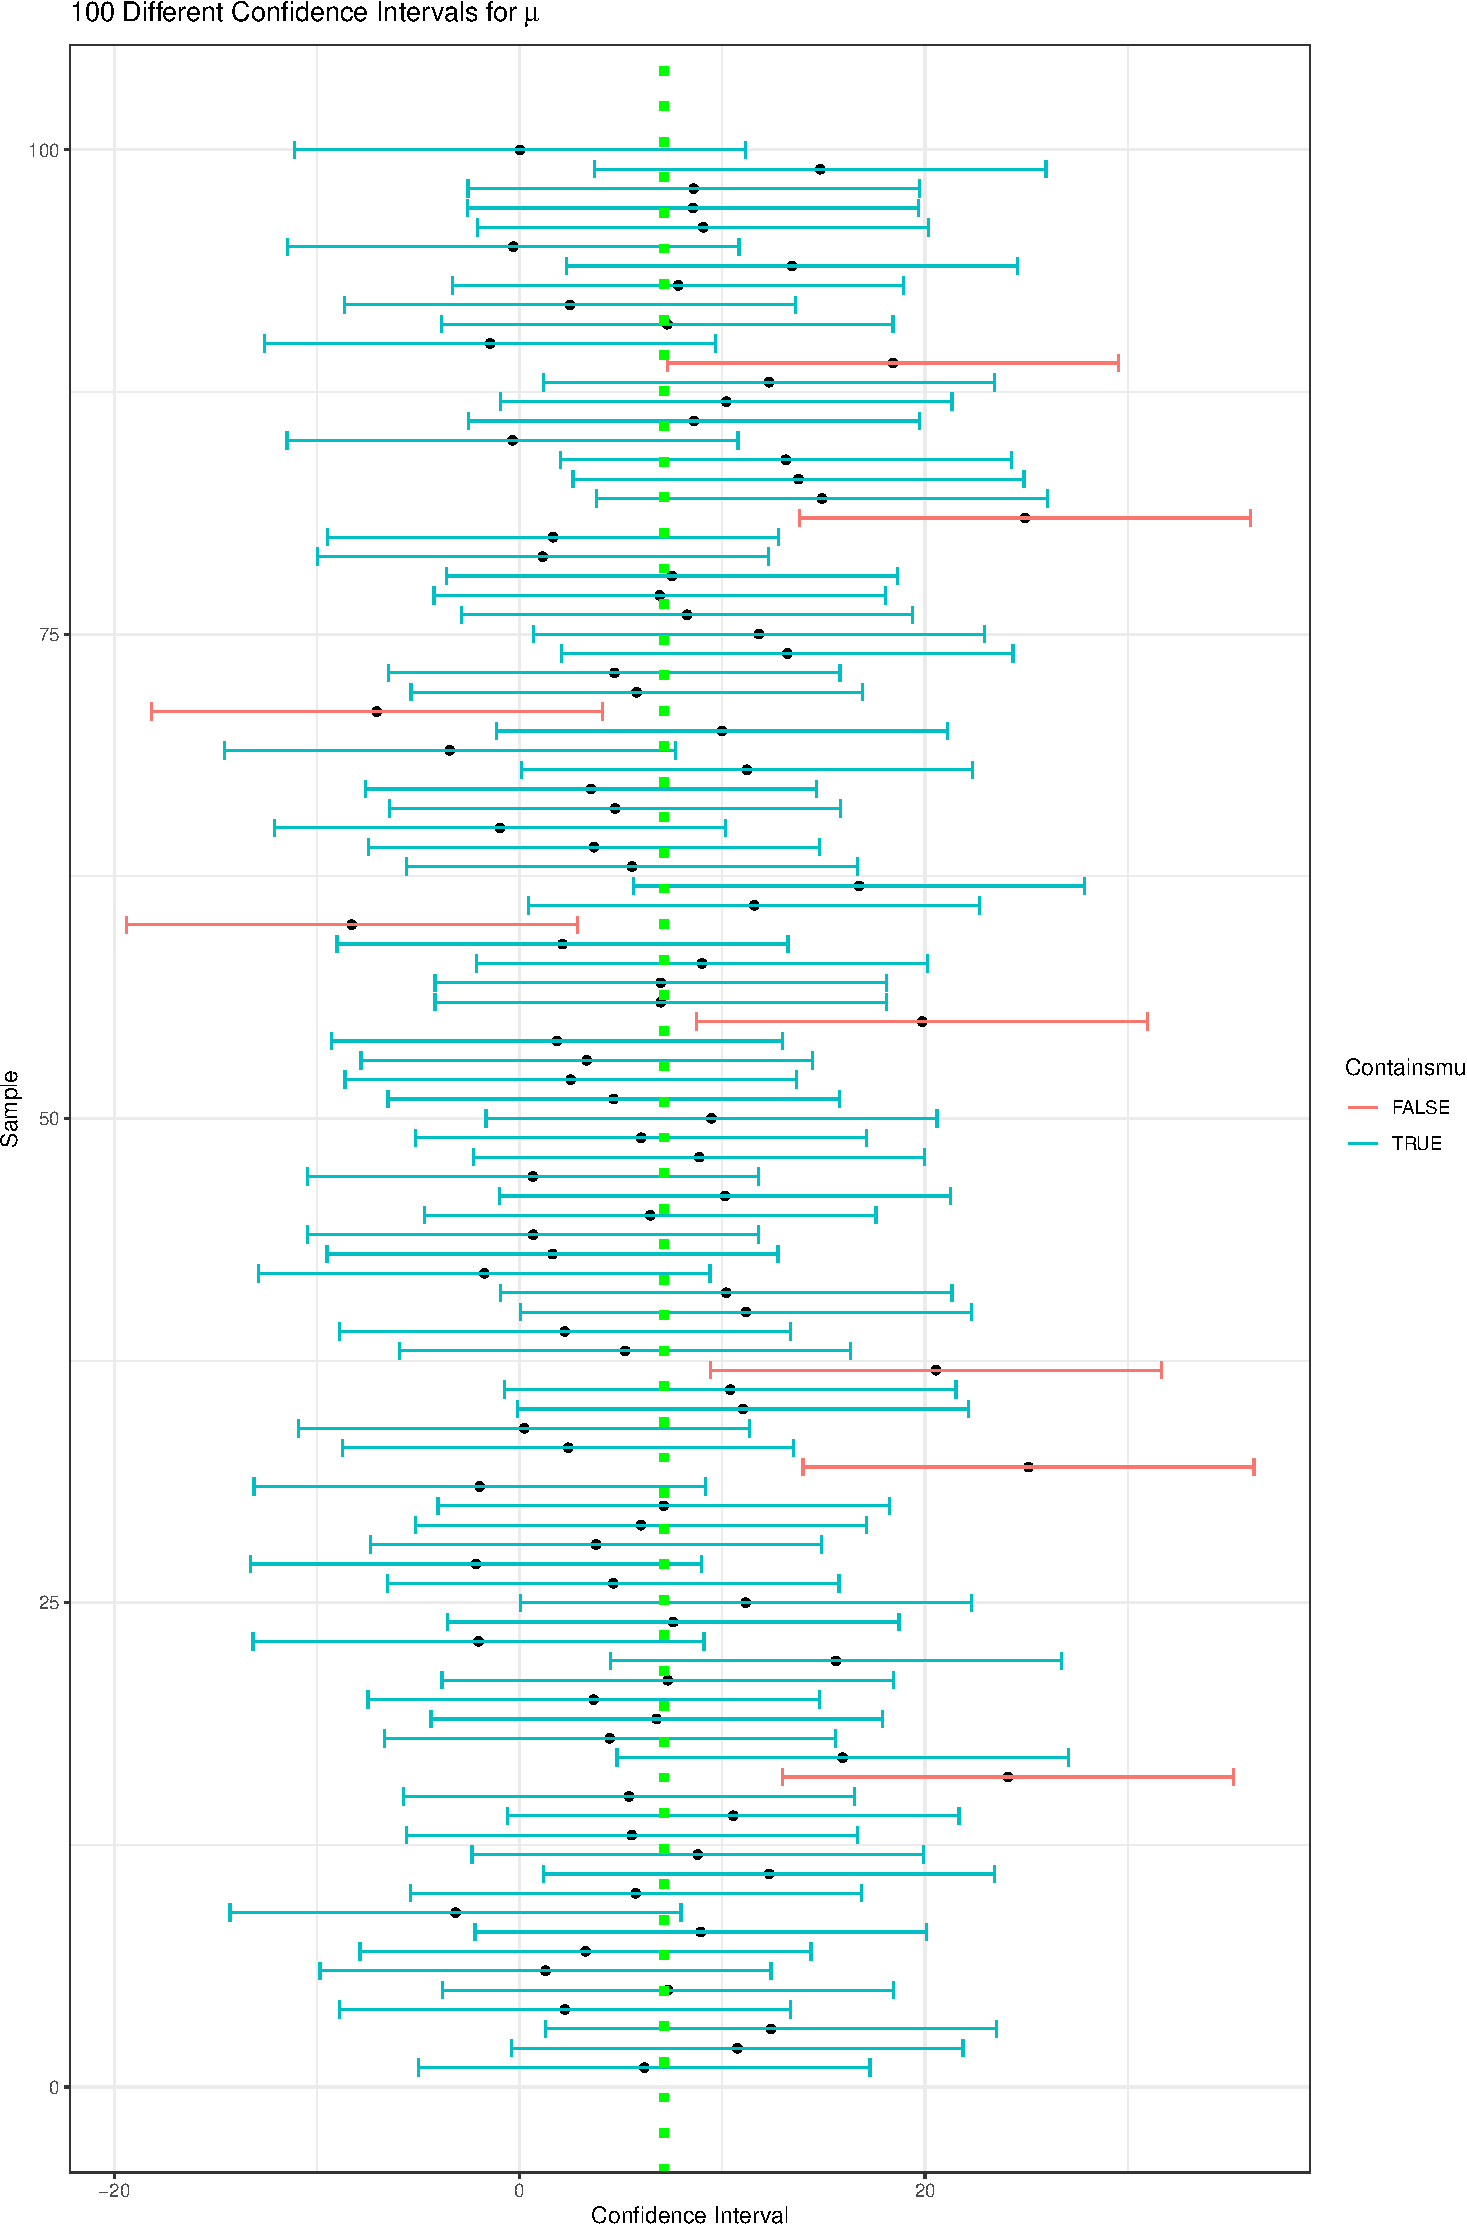
\includegraphics{Ch3_files/figure-pdf/unnamed-chunk-40-1.pdf}

Out of these 100 samples, 92 contain the true value of the population
parameter \(\mu\).

Out of all 10,000 samples, the proportion containing the true population
value of \(\mu\) is:

\begin{Shaded}
\begin{Highlighting}[]
\FunctionTok{sum}\NormalTok{(Samples\_df\_mu}\SpecialCharTok{$}\NormalTok{Containsmu }\SpecialCharTok{==} \ConstantTok{TRUE}\NormalTok{)}
\end{Highlighting}
\end{Shaded}

\begin{verbatim}
[1] 9570
\end{verbatim}

This brings us back to the question ``what does 95\% confidence mean?''.
An approximate 95\% confidence interval means that if we take a large
number of samples and calculate confidence intervals from each of them,
then approximately 95\% of the samples will produce intervals containing
the true population parameter. In reality, we'll only have on sample,
and won't know whether or not our interval contains the true parameter
value. Assuming we have taken the sample and calculated the interval
correctly, we can rest assured in the knowledge that that 95\% of all
intervals taken would contain the true parameter value, and hope that
ours is among that 95\%.

It might be tempting to say that ``there is approximately a 95\%
chance'' that the population parameter lies within the confidence
interval, but this is incorrect. In the statistical framework used here
(known as classical, or frequentist statistics), the population
parameter is assumed to be a fixed, but (typically) unknown number. It
either is within the interval, or it isn't. We just (typically) don't
know which. There's nothing random about whether or not the parameter
value is in our interval, so it doesn't make sense to speak of it in
terms of chance or randomness. Randomness comes into play due to the
fact that we selected a random sample, which will produce a statistic
likely to differ from the population parameter due to sampling
variability. A different statistical framework, known as \emph{Bayesian
statistics} approaches this differently, and would allow us to use
randomness and chance to describe our beliefs about any uncertain
quantity, including a population proportion. In this class, however,
we'll stick to the classical frequentist interpretation.

Of course, you might ask why we needed to calculate a confidence
interval for the proportion of on-time flights in the first place, since
we actually have data on all 20,591 flights in the population and
already know the true proportion of on-time arrivals and mean arrival
delay. The answer is that we don't. But, in most real situations, we
will only have data from a single sample, not the entire population, and
we won't know the true population parameter. We'll be able to build on
the ideas of sampling distributions and standard error that we learned
about in this section to calculate confidence intervals in those
scenarios.

\section{Bootstrapping}\label{bootstrapping}

\subsection{Mercury Concentration in Florida
Lakes}\label{mercury-concentration-in-florida-lakes}

A 2004 study by Lange, T., Royals, H. and Connor, L. examined Mercury
accumulation in large-mouth bass, taken from a sample of 53 Florida
Lakes. If Mercury accumulation exceeds 0.5 ppm, then there are
environmental concerns. In fact, the legal safety limit in Canada is 0.5
ppm, although it is 1 ppm in the United States.

In our sample, we have data on 53 lakes, out of more than 30,000 lakes
in the the state of Florida. We'll attempt to draw conclusions about the
entire population, consisting of all lakes in Florida, using data from
our sample of 53. It is not clear how the lakes in this sample of 53
were selected, or how representative they are of all lakes in the state
of Florida. Let's assume for our purposes that the lakes in the sample
can be reasonably thought of as being representative of all lakes in
Florida.

\begin{figure}[H]

{\centering 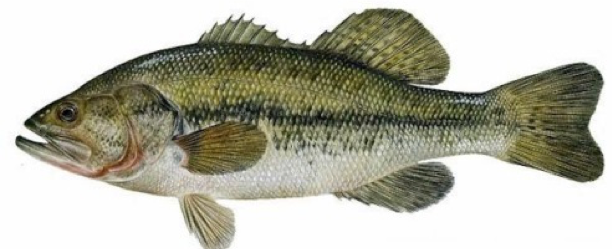
\includegraphics[width=0.5\textwidth,height=\textheight]{Bass.png}

}

\caption{https://www.maine.gov/ifw/fish-wildlife/fisheries/species-information/largemouth-bass.html}

\end{figure}%

\begin{Shaded}
\begin{Highlighting}[]
\FunctionTok{data}\NormalTok{(}\StringTok{"FloridaLakes"}\NormalTok{)}
\FunctionTok{glimpse}\NormalTok{(FloridaLakes)}
\end{Highlighting}
\end{Shaded}

\begin{verbatim}
Rows: 53
Columns: 12
$ ID                <int> 1, 2, 3, 4, 5, 6, 7, 8, 9, 10, 11, 12, 13, 14, 15, 1~
$ Lake              <chr> "Alligator", "Annie", "Apopka", "Blue Cypress", "Bri~
$ Alkalinity        <dbl> 5.9, 3.5, 116.0, 39.4, 2.5, 19.6, 5.2, 71.4, 26.4, 4~
$ pH                <dbl> 6.1, 5.1, 9.1, 6.9, 4.6, 7.3, 5.4, 8.1, 5.8, 6.4, 5.~
$ Calcium           <dbl> 3.0, 1.9, 44.1, 16.4, 2.9, 4.5, 2.8, 55.2, 9.2, 4.6,~
$ Chlorophyll       <dbl> 0.7, 3.2, 128.3, 3.5, 1.8, 44.1, 3.4, 33.7, 1.6, 22.~
$ AvgMercury        <dbl> 1.23, 1.33, 0.04, 0.44, 1.20, 0.27, 0.48, 0.19, 0.83~
$ NumSamples        <int> 5, 7, 6, 12, 12, 14, 10, 12, 24, 12, 12, 12, 7, 43, ~
$ MinMercury        <dbl> 0.85, 0.92, 0.04, 0.13, 0.69, 0.04, 0.30, 0.08, 0.26~
$ MaxMercury        <dbl> 1.43, 1.90, 0.06, 0.84, 1.50, 0.48, 0.72, 0.38, 1.40~
$ ThreeYrStdMercury <dbl> 1.53, 1.33, 0.04, 0.44, 1.33, 0.25, 0.45, 0.16, 0.72~
$ AgeData           <int> 1, 0, 0, 0, 1, 1, 1, 1, 1, 1, 1, 1, 1, 1, 0, 1, 1, 1~
\end{verbatim}

We are interested in whether mercury levels are higher or lower, on
average, in Northern Florida compared to Southern Florida.

We'll divide the state along route 50, which runs East-West, passing
through Northern Orlando.

\begin{figure}[H]

{\centering 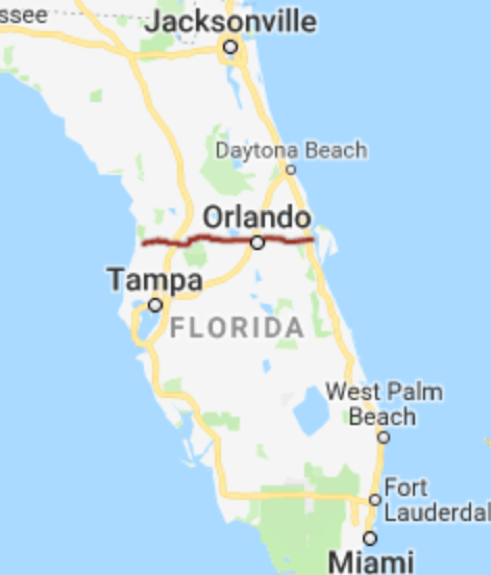
\includegraphics[width=0.3\textwidth,height=\textheight]{Florida.png}

}

\caption{from Google Maps}

\end{figure}%

We add a variable indicating whether each lake lies in the northern or
southern part of the state.

\begin{Shaded}
\begin{Highlighting}[]
\FunctionTok{library}\NormalTok{(Lock5Data)}
\FunctionTok{data}\NormalTok{(FloridaLakes)}
\CommentTok{\#Location relative to rt. 50}
\NormalTok{FloridaLakes}\SpecialCharTok{$}\NormalTok{Location }\OtherTok{\textless{}{-}} \FunctionTok{as.factor}\NormalTok{(}\FunctionTok{c}\NormalTok{(}\StringTok{"S"}\NormalTok{,}\StringTok{"S"}\NormalTok{,}\StringTok{"N"}\NormalTok{,}\StringTok{"S"}\NormalTok{,}\StringTok{"S"}\NormalTok{,}\StringTok{"N"}\NormalTok{,}\StringTok{"N"}\NormalTok{,}\StringTok{"N"}\NormalTok{,}\StringTok{"N"}\NormalTok{,}\StringTok{"N"}\NormalTok{,}\StringTok{"N"}\NormalTok{,}\StringTok{"S"}\NormalTok{,}\StringTok{"N"}\NormalTok{,}\StringTok{"S"}\NormalTok{,}\StringTok{"N"}\NormalTok{,}\StringTok{"N"}\NormalTok{,}\StringTok{"N"}\NormalTok{,}\StringTok{"N"}\NormalTok{,}\StringTok{"S"}\NormalTok{,}\StringTok{"S"}\NormalTok{,}\StringTok{"N"}\NormalTok{,}\StringTok{"S"}\NormalTok{,}\StringTok{"N"}\NormalTok{,}\StringTok{"S"}\NormalTok{,}\StringTok{"N"}\NormalTok{,}\StringTok{"S"}\NormalTok{,}\StringTok{"N"}\NormalTok{,}\StringTok{"S"}\NormalTok{,}\StringTok{"N"}\NormalTok{,}\StringTok{"N"}\NormalTok{,}\StringTok{"N"}\NormalTok{,}\StringTok{"N"}\NormalTok{,}\StringTok{"N"}\NormalTok{,}\StringTok{"N"}\NormalTok{,}\StringTok{"S"}\NormalTok{,}\StringTok{"N"}\NormalTok{,}\StringTok{"N"}\NormalTok{,}\StringTok{"S"}\NormalTok{,}\StringTok{"S"}\NormalTok{,}\StringTok{"N"}\NormalTok{,}\StringTok{"N"}\NormalTok{,}\StringTok{"N"}\NormalTok{,}\StringTok{"N"}\NormalTok{,}\StringTok{"S"}\NormalTok{,}\StringTok{"N"}\NormalTok{,}\StringTok{"S"}\NormalTok{,}\StringTok{"S"}\NormalTok{,}\StringTok{"S"}\NormalTok{,}\StringTok{"S"}\NormalTok{,}\StringTok{"N"}\NormalTok{,}\StringTok{"N"}\NormalTok{,}\StringTok{"N"}\NormalTok{,}\StringTok{"N"}\NormalTok{))}
\NormalTok{FloridaLakes }\OtherTok{\textless{}{-}}\NormalTok{ FloridaLakes }\SpecialCharTok{\%\textgreater{}\%} \FunctionTok{rename}\NormalTok{(}\AttributeTok{Mercury =}\NormalTok{ AvgMercury)}
\end{Highlighting}
\end{Shaded}

Our data come from a sample of 53 lakes, out of more then 30,000 in the
entire state of Florida. The mercury levels of the 53 lakes in the
sample are shown in the table below.

\begin{Shaded}
\begin{Highlighting}[]
\FunctionTok{print.data.frame}\NormalTok{(}\FunctionTok{data.frame}\NormalTok{(FloridaLakes}\SpecialCharTok{\%\textgreater{}\%} \FunctionTok{select}\NormalTok{(Lake, Location, Mercury)), }\AttributeTok{row.names =} \ConstantTok{FALSE}\NormalTok{)}
\end{Highlighting}
\end{Shaded}

\begin{verbatim}
              Lake Location Mercury
         Alligator        S    1.23
             Annie        S    1.33
            Apopka        N    0.04
      Blue Cypress        S    0.44
             Brick        S    1.20
            Bryant        N    0.27
            Cherry        N    0.48
          Crescent        N    0.19
        Deer Point        N    0.83
              Dias        N    0.81
              Dorr        N    0.71
              Down        S    0.50
             Eaton        N    0.49
 East Tohopekaliga        S    1.16
           Farm-13        N    0.05
            George        N    0.15
           Griffin        N    0.19
            Harney        N    0.77
              Hart        S    1.08
        Hatchineha        S    0.98
           Iamonia        N    0.63
         Istokpoga        S    0.56
           Jackson        N    0.41
         Josephine        S    0.73
          Kingsley        N    0.34
         Kissimmee        S    0.59
         Lochloosa        N    0.34
            Louisa        S    0.84
        Miccasukee        N    0.50
          Minneola        N    0.34
            Monroe        N    0.28
           Newmans        N    0.34
        Ocean Pond        N    0.87
      Ocheese Pond        N    0.56
        Okeechobee        S    0.17
            Orange        N    0.18
       Panasoffkee        N    0.19
            Parker        S    0.04
            Placid        S    0.49
            Puzzle        N    1.10
            Rodman        N    0.16
          Rousseau        N    0.10
           Sampson        N    0.48
             Shipp        S    0.21
           Talquin        N    0.86
            Tarpon        S    0.52
      Tohopekaliga        S    0.65
          Trafford        S    0.27
             Trout        S    0.94
      Tsala Apopka        N    0.40
              Weir        N    0.43
           Wildcat        N    0.25
              Yale        N    0.27
\end{verbatim}

The histogram shows the distribution of mercury levels in the 53 lakes
in the sample. Lakes exceeding the US standard of 1 ppm are shown in
red.

\begin{Shaded}
\begin{Highlighting}[]
\NormalTok{Lakes\_Hist }\OtherTok{\textless{}{-}} \FunctionTok{ggplot}\NormalTok{(}\AttributeTok{data=}\NormalTok{FloridaLakes, }\FunctionTok{aes}\NormalTok{(}\AttributeTok{x=}\NormalTok{Mercury)) }\SpecialCharTok{+} 
  \FunctionTok{geom\_histogram}\NormalTok{(}\FunctionTok{aes}\NormalTok{(}\AttributeTok{fill=}\NormalTok{Mercury}\SpecialCharTok{\textless{}=}\DecValTok{1}\NormalTok{), }\AttributeTok{color=}\StringTok{"white"}\NormalTok{, }\AttributeTok{binwidth =} \FloatTok{0.1}\NormalTok{) }\SpecialCharTok{+} 
  \FunctionTok{ggtitle}\NormalTok{(}\StringTok{"Mercury Levels in Sample of 53 Florida Lakes"}\NormalTok{) }\SpecialCharTok{+} 
  \FunctionTok{xlab}\NormalTok{(}\StringTok{"Mercury Level"}\NormalTok{) }\SpecialCharTok{+} \FunctionTok{ylab}\NormalTok{(}\StringTok{"Frequency"}\NormalTok{) }\SpecialCharTok{+} \FunctionTok{theme\_bw}\NormalTok{()}
\NormalTok{Lakes\_Hist}
\end{Highlighting}
\end{Shaded}

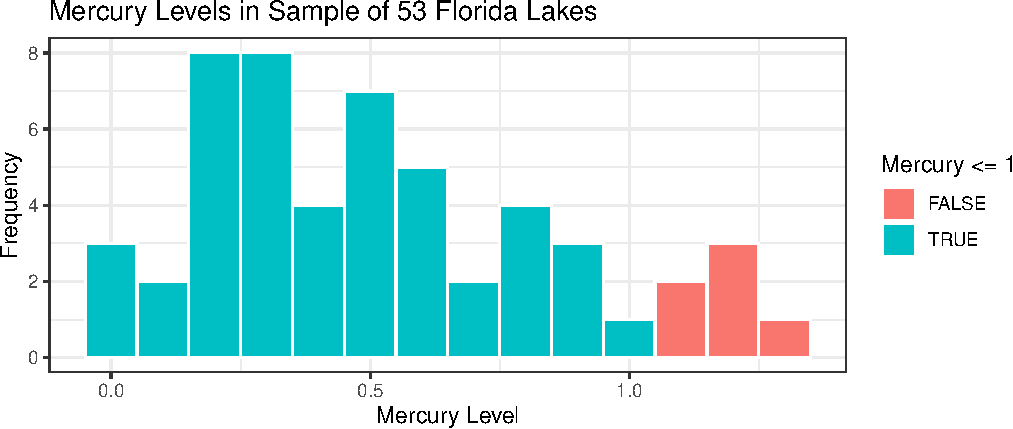
\includegraphics{Ch3_files/figure-pdf/unnamed-chunk-46-1.pdf}

The proportion of lakes with mercury levels exceeding 1 ppm is
calculated below.

\begin{Shaded}
\begin{Highlighting}[]
\NormalTok{p\_hat }\OtherTok{\textless{}{-}} \FunctionTok{sum}\NormalTok{(FloridaLakes}\SpecialCharTok{$}\NormalTok{Mercury }\SpecialCharTok{\textgreater{}} \DecValTok{1}\NormalTok{)}\SpecialCharTok{/}\DecValTok{53}
\NormalTok{p\_hat}
\end{Highlighting}
\end{Shaded}

\begin{verbatim}
[1] 0.1132075
\end{verbatim}

We see that in our sample of 53 lakes, approximately 11\% have mercury
levels exceeding the US standard of 1 ppm. Suppose we want to estimate
the proportion of all Florida Lakes whose mercury level exceeds this
standard. As we saw in the previous section, we would not expect the
population proportion to exactly match the sample, due to random
variability between samples. We can use the sample proportion as an
estimate (\(\hat{p} = 0.1132\)), and construct a confidence interval for
the unknown population proportion \(p\).

In order to construct the confidence interval, we need to know how much
the sample proportion of lakes exceeding 1 ppm \(\hat{p}\) could vary
between different samples of size 53. That is, we need to know the
standard error of \(\hat{p}\). In the previous section, we calculated
the standard error by taking 10,000 different samples of the same size
as ours from the population, calculating the proportion for each sample,
and then calculating the standard deviation of the proportions obtained
from these 10,000 different samples. This procedure will not work here,
however, because unlike the previous example where we really did have
data on the entire population of all flights from New York to Chicago,
we do not have data on all 30,000+ lakes in Florida. We cannot take a
lot of different samples of size 53 from the population of all lakes,
and thus, cannot obtain the sampling distribution for the the proportion
of lakes exceeding 1 ppm, or estimate the standard error of \(\hat{p}\).

\subsection{Bootstrap Sampling}\label{bootstrap-sampling}

All we have is a single sample of 53 lakes. We need to figure out how
much the proportion of lakes with mercury levels exceeding 1 ppm would
vary between different samples of size 53, using only the information
contained in our one sample.

To do this, we'll implement a popular simulation-based strategy, known
as \textbf{bootstrapping}.

Let's assume our sample is representative of all Florida lakes. Then,
we'll duplicate the sample many times to create a large set that will
look like the population of all Florida Lakes. We can then draw samples
of 53 from that large population, and record the mean mercury level for
each sample of 53.

An illustration of the bootstrapping procedure is shown below, using a
sample of 12 colored dots, instead of the 53 lakes.

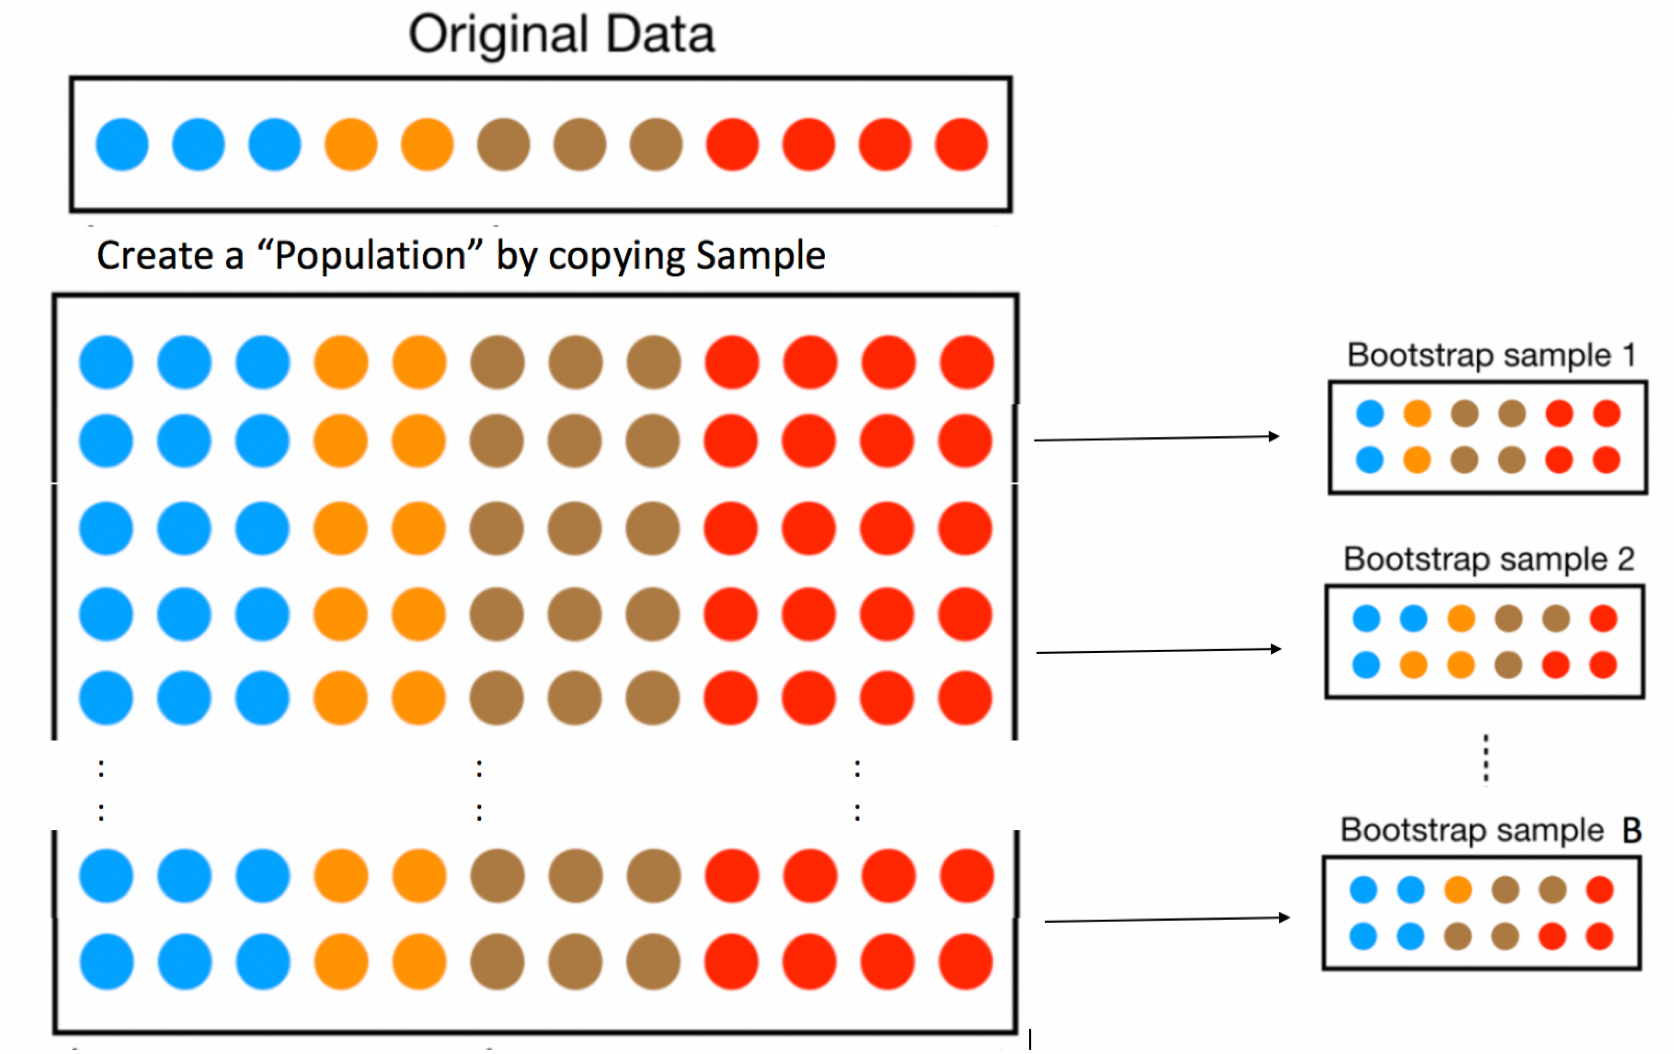
\includegraphics[width=1\textwidth,height=\textheight]{Bootstrap_Idea.png}

In fact, duplicating the sample many times and selecting new samples of
size \(n\) has the same effect as drawing samples of size \(n\) from the
original sample, by putting the item drawn back in each time, a
procedure called \textbf{sampling with replacement}. Thus, we can skip
the step of copying/pasting the sample many times, and instead draw our
samples with replacement.

This means that in each new sample, some lakes will be drawn multiple
times and others not at all. It also ensures that each sample is
different, allowing us to estimate variability in the sample mean
between the different samples of size 53.

An illustration of the concept of bootstrapping, using sampling with
replacement is shown below.

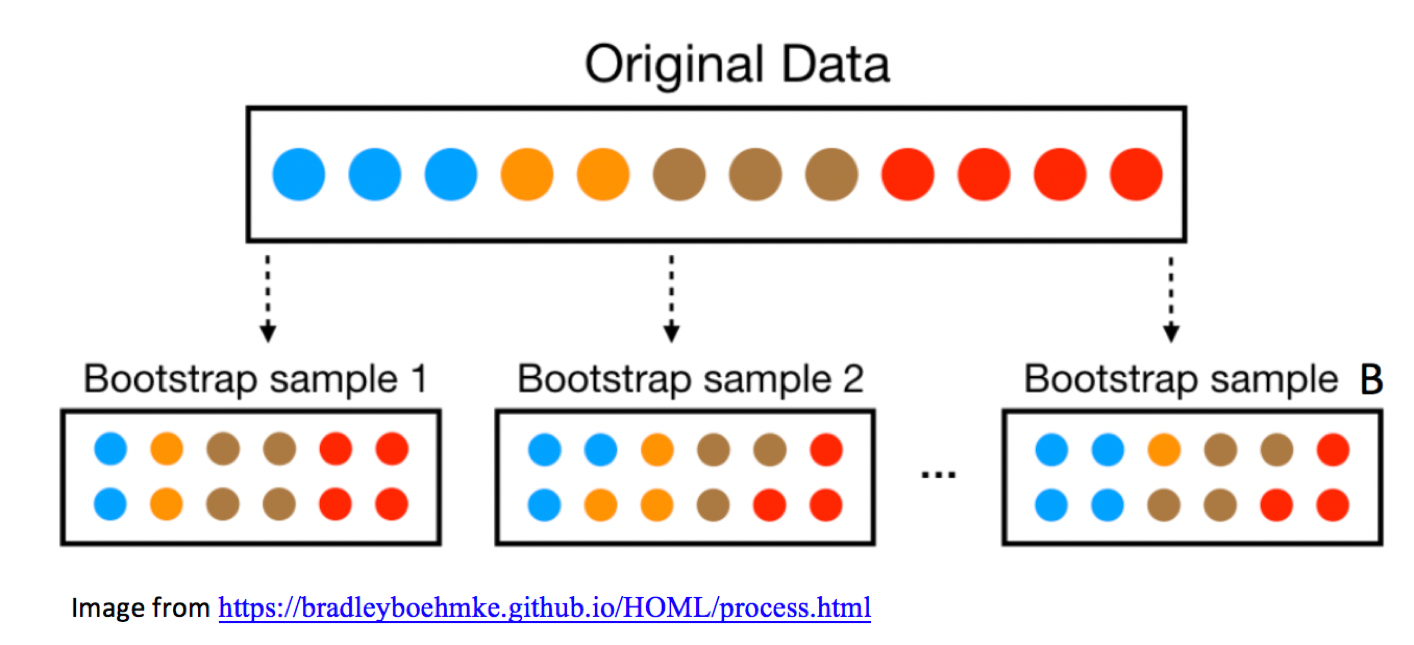
\includegraphics[width=1\textwidth,height=\textheight]{Bootstrap.png}

The variability in sample means in our newly drawn samples is used to
approximate the variability in proportion \(\hat{p}\) that would occur
between different samples of 53 lakes, drawn from the population of all
Florida Lakes.

The point of bootstrapping is to observe how much a statistic (in this
case the proportion of lakes with Mercury levels exceeding 1 ppm) varies
between bootstrap samples. This can act as an estimate of how much that
statistic would vary between different samples of size \(n\), drawn from
the population.

The steps of bootstrap sampling can be summarized in the following
algorithm.

\textbf{Bootstrap Algorithm}

For an original sample of size \(n\):

\begin{enumerate}
\def\labelenumi{\arabic{enumi}.}
\item
  Take a sample size \(n\) by randomly sampling from the original, with
  replacement. Thus, some observations will show up multiple times, and
  others not at all. This sample is called a \textbf{bootstrap sample}.
\item
  Calculate the statistic of interest in the bootstrap sample (in this
  case \(\hat{p}\), the proportion of lakes whose mercury levels exceed
  1 ppm).
\item
  Repeat steps 1 and 2 many (say 10,000) times, keeping track of the
  statistic of interest that is calculated in each bootstrap sample.
\item
  Look at the distribution of the statistic across bootstrap samples.
  The variability in this bootstrap distribution can be used to
  approximate the variability in the sampling distribution for the
  statistic of interest.
\end{enumerate}

\subsection{Bootstrap Samples of
Lakes}\label{bootstrap-samples-of-lakes}

The \texttt{sample\_n()} function samples the specified number rows from
a data frame, with or without replacement.

The lakes in the first sample are shown below. Notice that some lakes
occur multiple times, and others not at all.

\textbf{Bootstrap Sample 1}

\begin{Shaded}
\begin{Highlighting}[]
\NormalTok{BootstrapSample1 }\OtherTok{\textless{}{-}} \FunctionTok{sample\_n}\NormalTok{(FloridaLakes, }\DecValTok{53}\NormalTok{, }\AttributeTok{replace=}\ConstantTok{TRUE}\NormalTok{) }\SpecialCharTok{\%\textgreater{}\%} \FunctionTok{arrange}\NormalTok{(Lake)}
\NormalTok{BootstrapSample1 }\SpecialCharTok{\%\textgreater{}\%} \FunctionTok{select}\NormalTok{(ID, Lake, Mercury) }\SpecialCharTok{|\textgreater{}} \FunctionTok{kable}\NormalTok{()}
\end{Highlighting}
\end{Shaded}

\begin{longtable}[]{@{}rlr@{}}
\toprule\noalign{}
ID & Lake & Mercury \\
\midrule\noalign{}
\endhead
\bottomrule\noalign{}
\endlastfoot
3 & Apopka & 0.04 \\
4 & Blue Cypress & 0.44 \\
4 & Blue Cypress & 0.44 \\
5 & Brick & 1.20 \\
5 & Brick & 1.20 \\
5 & Brick & 1.20 \\
6 & Bryant & 0.27 \\
6 & Bryant & 0.27 \\
7 & Cherry & 0.48 \\
10 & Dias & 0.81 \\
10 & Dias & 0.81 \\
10 & Dias & 0.81 \\
13 & Eaton & 0.49 \\
17 & Griffin & 0.19 \\
18 & Harney & 0.77 \\
18 & Harney & 0.77 \\
19 & Hart & 1.08 \\
20 & Hatchineha & 0.98 \\
22 & Istokpoga & 0.56 \\
22 & Istokpoga & 0.56 \\
23 & Jackson & 0.41 \\
25 & Kingsley & 0.34 \\
25 & Kingsley & 0.34 \\
26 & Kissimmee & 0.59 \\
27 & Lochloosa & 0.34 \\
30 & Minneola & 0.34 \\
32 & Newmans & 0.34 \\
33 & Ocean Pond & 0.87 \\
34 & Ocheese Pond & 0.56 \\
35 & Okeechobee & 0.17 \\
37 & Panasoffkee & 0.19 \\
37 & Panasoffkee & 0.19 \\
38 & Parker & 0.04 \\
38 & Parker & 0.04 \\
40 & Puzzle & 1.10 \\
40 & Puzzle & 1.10 \\
40 & Puzzle & 1.10 \\
41 & Rodman & 0.16 \\
41 & Rodman & 0.16 \\
42 & Rousseau & 0.10 \\
43 & Sampson & 0.48 \\
43 & Sampson & 0.48 \\
44 & Shipp & 0.21 \\
44 & Shipp & 0.21 \\
45 & Talquin & 0.86 \\
51 & Tohopekaliga & 0.65 \\
51 & Tohopekaliga & 0.65 \\
51 & Tohopekaliga & 0.65 \\
48 & Trout & 0.94 \\
48 & Trout & 0.94 \\
52 & Wildcat & 0.25 \\
52 & Wildcat & 0.25 \\
53 & Yale & 0.27 \\
\end{longtable}

We calculate the proportion of lakes with mercury levels exceeding 1 ppm
in this bootstrap sample. Note that if a lake shows up more than once in
the bootstrap sample, then it is counted however many times it shows up.

\begin{Shaded}
\begin{Highlighting}[]
\FunctionTok{sum}\NormalTok{(BootstrapSample1}\SpecialCharTok{$}\NormalTok{Mercury }\SpecialCharTok{\textgreater{}} \DecValTok{1}\NormalTok{) }\SpecialCharTok{/} \DecValTok{53}
\end{Highlighting}
\end{Shaded}

\begin{verbatim}
[1] 0.1320755
\end{verbatim}

\textbf{Bootstrap Sample \#2}

We take a second bootstrap sample. We display only the first 10 lakes,
though the bootstrap sample still has 53 lakes.

Notice that the lakes chosen and omitted differ from the first sample.

\begin{Shaded}
\begin{Highlighting}[]
\NormalTok{BootstrapSample2 }\OtherTok{\textless{}{-}} \FunctionTok{sample\_n}\NormalTok{(FloridaLakes, }\DecValTok{53}\NormalTok{, }\AttributeTok{replace=}\ConstantTok{TRUE}\NormalTok{) }\SpecialCharTok{\%\textgreater{}\%} \FunctionTok{arrange}\NormalTok{(Lake)}
\NormalTok{BootstrapSample2 }\SpecialCharTok{\%\textgreater{}\%} \FunctionTok{select}\NormalTok{(ID, Lake, Mercury)}
\end{Highlighting}
\end{Shaded}

\begin{verbatim}
# A tibble: 53 x 3
      ID Lake         Mercury
   <int> <chr>          <dbl>
 1     1 Alligator       1.23
 2     3 Apopka          0.04
 3     4 Blue Cypress    0.44
 4     5 Brick           1.2 
 5     6 Bryant          0.27
 6     7 Cherry          0.48
 7     9 Deer Point      0.83
 8    10 Dias            0.81
 9    10 Dias            0.81
10    11 Dorr            0.71
# i 43 more rows
\end{verbatim}

Proportion exceeding 1 ppm:

\begin{Shaded}
\begin{Highlighting}[]
\FunctionTok{sum}\NormalTok{(BootstrapSample2}\SpecialCharTok{$}\NormalTok{Mercury }\SpecialCharTok{\textgreater{}} \DecValTok{1}\NormalTok{) }\SpecialCharTok{/} \DecValTok{53}
\end{Highlighting}
\end{Shaded}

\begin{verbatim}
[1] 0.0754717
\end{verbatim}

\textbf{Bootstrap Sample \#3}

We'll take one more bootstrap sample and calculate the proportion of
lakes with mercury levels exceeding 1 ppm. The first 10 lakes in this
third sample are shown.

\begin{Shaded}
\begin{Highlighting}[]
\NormalTok{BootstrapSample3 }\OtherTok{\textless{}{-}} \FunctionTok{sample\_n}\NormalTok{(FloridaLakes, }\DecValTok{53}\NormalTok{, }\AttributeTok{replace=}\ConstantTok{TRUE}\NormalTok{) }\SpecialCharTok{\%\textgreater{}\%} \FunctionTok{arrange}\NormalTok{(Lake)}
\NormalTok{BootstrapSample3 }\SpecialCharTok{\%\textgreater{}\%} \FunctionTok{select}\NormalTok{(ID, Lake, Mercury)}
\end{Highlighting}
\end{Shaded}

\begin{verbatim}
# A tibble: 53 x 3
      ID Lake       Mercury
   <int> <chr>        <dbl>
 1     1 Alligator     1.23
 2     3 Apopka        0.04
 3     3 Apopka        0.04
 4     5 Brick         1.2 
 5     5 Brick         1.2 
 6     7 Cherry        0.48
 7     7 Cherry        0.48
 8     8 Crescent      0.19
 9     9 Deer Point    0.83
10    10 Dias          0.81
# i 43 more rows
\end{verbatim}

Proportion exceeding 1 ppm:

\begin{Shaded}
\begin{Highlighting}[]
\FunctionTok{sum}\NormalTok{(BootstrapSample3}\SpecialCharTok{$}\NormalTok{Mercury }\SpecialCharTok{\textgreater{}} \DecValTok{1}\NormalTok{) }\SpecialCharTok{/} \DecValTok{53}
\end{Highlighting}
\end{Shaded}

\begin{verbatim}
[1] 0.1132075
\end{verbatim}

\subsection{Bootstrap Distribution}\label{bootstrap-distribution}

Now that we have seen how bootstrap sampling works, we'll take a large
number (10,000) different bootstrap samples and examine how the
proportion of lakes with mercury levels exceeding 1 ppm varies between
samples.

We'll use a \texttt{for-loop} to take many different bootstrap samples
and record the observed proportion in a vector called \texttt{p\_hat\_b}

\begin{Shaded}
\begin{Highlighting}[]
\NormalTok{p\_hat }\OtherTok{\textless{}{-}} \FunctionTok{sum}\NormalTok{(FloridaLakes}\SpecialCharTok{$}\NormalTok{Mercury }\SpecialCharTok{\textgreater{}} \DecValTok{1}\NormalTok{)}\SpecialCharTok{/}\DecValTok{53} \CommentTok{\#calculate sample statistic}
\NormalTok{Bootstrap\_prop }\OtherTok{\textless{}{-}} \FunctionTok{rep}\NormalTok{(}\ConstantTok{NA}\NormalTok{, }\DecValTok{10000}\NormalTok{)   }\CommentTok{\#setup vector to hold bootstrap statistics}

\ControlFlowTok{for}\NormalTok{ (i }\ControlFlowTok{in} \DecValTok{1}\SpecialCharTok{:}\DecValTok{10000}\NormalTok{)\{}
\NormalTok{BootstrapSample }\OtherTok{\textless{}{-}} \FunctionTok{sample\_n}\NormalTok{(FloridaLakes, }\DecValTok{53}\NormalTok{, }\AttributeTok{replace=}\ConstantTok{TRUE}\NormalTok{) }\CommentTok{\#take bootstrap sample}
\NormalTok{Bootstrap\_prop[i] }\OtherTok{\textless{}{-}} \FunctionTok{sum}\NormalTok{(BootstrapSample}\SpecialCharTok{$}\NormalTok{Mercury }\SpecialCharTok{\textgreater{}} \DecValTok{1}\NormalTok{)}\SpecialCharTok{/}\DecValTok{53} \CommentTok{\# calc. prop exceeding 1}
\NormalTok{\}}
\NormalTok{Lakes\_Bootstrap\_Prop }\OtherTok{\textless{}{-}} \FunctionTok{data.frame}\NormalTok{(Bootstrap\_prop)  }\CommentTok{\#store values in a dataframe}
\end{Highlighting}
\end{Shaded}

The distribution of proportions observed in the 10,000 different
bootstrap samples is shown below. This distribution is called the
\textbf{bootstrap distribution.}

\begin{Shaded}
\begin{Highlighting}[]
\NormalTok{Lakes\_Bootstrap\_Prop\_plot }\OtherTok{\textless{}{-}} \FunctionTok{ggplot}\NormalTok{(}\AttributeTok{data=}\NormalTok{Lakes\_Bootstrap\_Prop, }\FunctionTok{aes}\NormalTok{(}\AttributeTok{x=}\NormalTok{Bootstrap\_prop)) }\SpecialCharTok{+}  
  \FunctionTok{geom\_histogram}\NormalTok{(}\AttributeTok{color=}\StringTok{"white"}\NormalTok{, }\AttributeTok{fill=}\StringTok{"lightblue"}\NormalTok{, }\AttributeTok{binwidth=}\FloatTok{0.02}\NormalTok{) }\SpecialCharTok{+}
  \FunctionTok{xlab}\NormalTok{(}\StringTok{"Prop \textgreater{} 1 in Bootstrap Sample "}\NormalTok{) }\SpecialCharTok{+} \FunctionTok{ylab}\NormalTok{(}\StringTok{"Frequency"}\NormalTok{) }\SpecialCharTok{+}
  \FunctionTok{ggtitle}\NormalTok{(}\StringTok{"Bootstrap Distribution for Prop. of Lakes Exeeding 1 ppm Hg"}\NormalTok{) }\SpecialCharTok{+} 
  \FunctionTok{theme}\NormalTok{(}\AttributeTok{legend.position =} \StringTok{"none"}\NormalTok{)}
\NormalTok{Lakes\_Bootstrap\_Prop\_plot}
\end{Highlighting}
\end{Shaded}

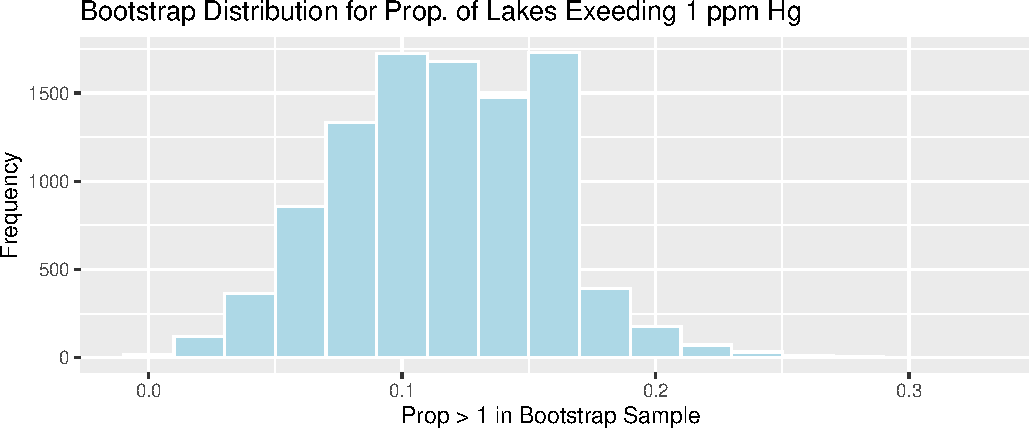
\includegraphics{Ch3_files/figure-pdf/unnamed-chunk-57-1.pdf}

The bootstrap distribution is meant to approximate the sampling
distribution of the statistic of interest (in this case the proportion
exceeding 1 ppm). Because it is based on the sample, the bootstrap
distribution will be centered at the sample statistic (\(\hat{p}\) in
this case) while the sampling distribution would have been centered at
the population parameter (\(p\)), which is unknown. The important
things, however, is that the variability in the bootstrap distribution
gives a good approximation of the amount of variability in the sampling
distribution, so we can use the standard deviation of the bootstrap
distribution (called \textbf{bootstrap standard error}) in our
confidence interval calculation.

\subsection{Bootstrap SE Confidence
Interval}\label{bootstrap-se-confidence-interval}

We calculate the standard deviation of this bootstrap distribution,
which is an estimate of the standard error of \(\hat{p}\). It measures
how much the proportion of lakes exceeding 1 ppm varies between samples
of size 53.

\textbf{Bootstrap Standard Error:}

\begin{Shaded}
\begin{Highlighting}[]
\NormalTok{SE\_p\_hat }\OtherTok{\textless{}{-}} \FunctionTok{sd}\NormalTok{(Lakes\_Bootstrap\_Prop}\SpecialCharTok{$}\NormalTok{Bootstrap\_prop)}
\end{Highlighting}
\end{Shaded}

Since the bootstrap distribution is roughly symmetric and bell-shaped,
we can calculate a 95\% confidence interval for the proportion of all
Florida lakes with mercury levels exceeding 1 ppm, using bootstrap
standard error confidence interval method.

\[
\hat{p} \pm 2\times\text{SE}(\hat{p})
\]

\begin{Shaded}
\begin{Highlighting}[]
\FunctionTok{c}\NormalTok{(p\_hat }\SpecialCharTok{{-}} \DecValTok{2}\SpecialCharTok{*}\NormalTok{SE\_p\_hat, p\_hat }\SpecialCharTok{+} \DecValTok{2}\SpecialCharTok{*}\NormalTok{SE\_p\_hat)}
\end{Highlighting}
\end{Shaded}

\begin{verbatim}
[1] 0.02684273 0.19957237
\end{verbatim}

The gold bar at the bottom of the bootstrap distribution represents this
95\% confidence interval.

\begin{Shaded}
\begin{Highlighting}[]
\NormalTok{Lakes\_Bootstrap\_Prop\_plot }\SpecialCharTok{+} 
  \FunctionTok{geom\_segment}\NormalTok{(}\FunctionTok{aes}\NormalTok{(}\AttributeTok{x=}\NormalTok{p\_hat }\SpecialCharTok{{-}} \DecValTok{2}\SpecialCharTok{*}\NormalTok{SE\_p\_hat,}\AttributeTok{xend=}\NormalTok{p\_hat }\SpecialCharTok{+} \DecValTok{2}\SpecialCharTok{*}\NormalTok{SE\_p\_hat, }\AttributeTok{y=}\DecValTok{50}\NormalTok{, }\AttributeTok{yend=}\DecValTok{50}\NormalTok{),}
               \AttributeTok{color=}\StringTok{"gold"}\NormalTok{, }\AttributeTok{size=}\DecValTok{10}\NormalTok{, }\AttributeTok{alpha=}\FloatTok{0.01}\NormalTok{) }
\end{Highlighting}
\end{Shaded}

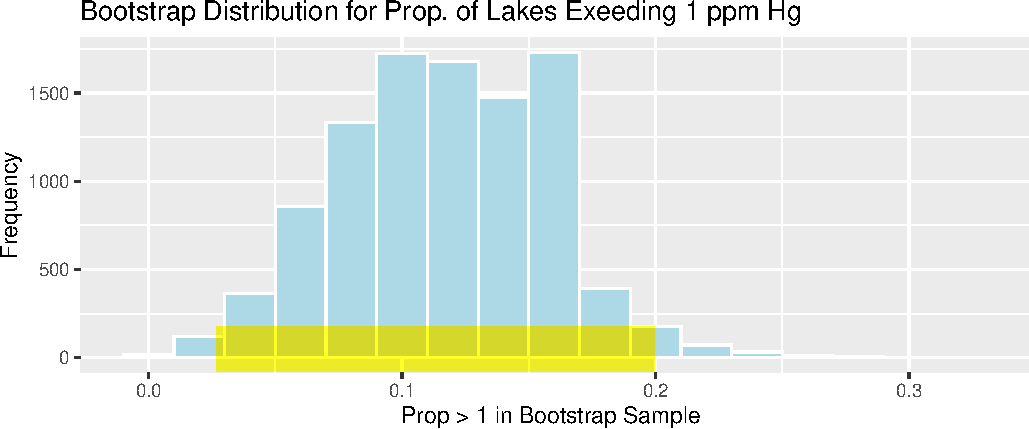
\includegraphics{Ch3_files/figure-pdf/unnamed-chunk-60-1.pdf}

We are 95\% confident that the proportion of all Florida lakes with
mercury levels exceeding 1 ppm is between 0.0268 and 0.1996.

\section{More Bootstrap Examples}\label{more-bootstrap-examples}

\subsection{Bootstrapping Other
Statistics}\label{bootstrapping-other-statistics}

We've seen how to use bootstrapping to calculate confidence intervals
for an unknown population parameter \(p\), using an estimate
\(\hat{p}\), calculated from a sample of size \(n\). This procedure can
be applied to calculate confidence intervals for a wide range of
population parameters, using statistics calculated from a sample.

For example, we could calculate confidence intervals any of the
following parameters, using the corresponding sample statistic.

\begin{longtable}[]{@{}
  >{\raggedright\arraybackslash}p{(\columnwidth - 4\tabcolsep) * \real{0.3611}}
  >{\raggedright\arraybackslash}p{(\columnwidth - 4\tabcolsep) * \real{0.3194}}
  >{\raggedright\arraybackslash}p{(\columnwidth - 4\tabcolsep) * \real{0.3194}}@{}}
\toprule\noalign{}
\begin{minipage}[b]{\linewidth}\raggedright
Context
\end{minipage} & \begin{minipage}[b]{\linewidth}\raggedright
Parameter
\end{minipage} & \begin{minipage}[b]{\linewidth}\raggedright
Statistic
\end{minipage} \\
\midrule\noalign{}
\endhead
\bottomrule\noalign{}
\endlastfoot
Proportion & \(p\) & \(\hat{p}\) \\
Mean & \(\mu\) & \(\bar{x}\) \\
Standard Deviation & \(\sigma\) & \(s\) \\
Median & no common abbreviations & \\
Difference in Means & \(\mu_2-\mu_1\) & \(\bar{x}_2 - \bar{x}_1\) \\
Regression Coefficient & \(\beta_j\) & \(b_j\) \\
Estimated Regression Response &
\(\beta_0 + \beta_1x_{i1} + \ldots + \beta_px_{ip}\) &
\(b_0 + b_1x_{i1} + \ldots + b_px_{ip}\) \\
\end{longtable}

We follow the same algorithm as we did when working with a proportion,
and simply calculate whatever statistic we are interested in step 2, in
place of \(\hat{p}\), as we did previously.

The bootstrap algorithm is given again, below.

\textbf{Bootstrap Algorithm}

For an original sample of size \(n\):

\begin{enumerate}
\def\labelenumi{\arabic{enumi}.}
\item
  Take a sample of size \(n\) by randomly sampling from the original
  sample with replacement. (Thus some observations will show up multiple
  times and others not at all.)
\item
  Calculate the statistic of interest in the bootstrap sample.
\item
  Repeat steps 1 and 2 many (say 10,000) times, keeping track of the
  statistic of interest that is calculated in each bootstrap sample.
\item
  Look at the distribution of the statistic across bootstrap samples.
  The variability in this bootstrap distribution can be used to
  approximate the variability in the sampling distribution for the
  statistic of interest.
\end{enumerate}

We'll now go through examples, calculating bootstrap confidence
intervals for each of the parameters listed above.

\subsection{CI for Mean}\label{ci-for-mean}

The histogram shows the distribution of mercury levels of the 53 lakes
in our sample. The mean and standard deviation in mercury levels for
these 53 lakes is shown.

\begin{Shaded}
\begin{Highlighting}[]
\NormalTok{Lakes\_Hist }\OtherTok{\textless{}{-}} \FunctionTok{ggplot}\NormalTok{(}\AttributeTok{data=}\NormalTok{FloridaLakes, }\FunctionTok{aes}\NormalTok{(}\AttributeTok{x=}\NormalTok{Mercury)) }\SpecialCharTok{+} 
  \FunctionTok{geom\_histogram}\NormalTok{(}\AttributeTok{color=}\StringTok{"white"}\NormalTok{, }\AttributeTok{fill=}\StringTok{"lightblue"}\NormalTok{, }\AttributeTok{binwidth =} \FloatTok{0.2}\NormalTok{) }\SpecialCharTok{+} 
  \FunctionTok{ggtitle}\NormalTok{(}\StringTok{"Mercury Levels in Sample of Florida Lakes"}\NormalTok{) }\SpecialCharTok{+} 
  \FunctionTok{xlab}\NormalTok{(}\StringTok{"Mercury Level"}\NormalTok{) }\SpecialCharTok{+} \FunctionTok{ylab}\NormalTok{(}\StringTok{"Frequency"}\NormalTok{) }
\NormalTok{Lakes\_Hist}
\end{Highlighting}
\end{Shaded}

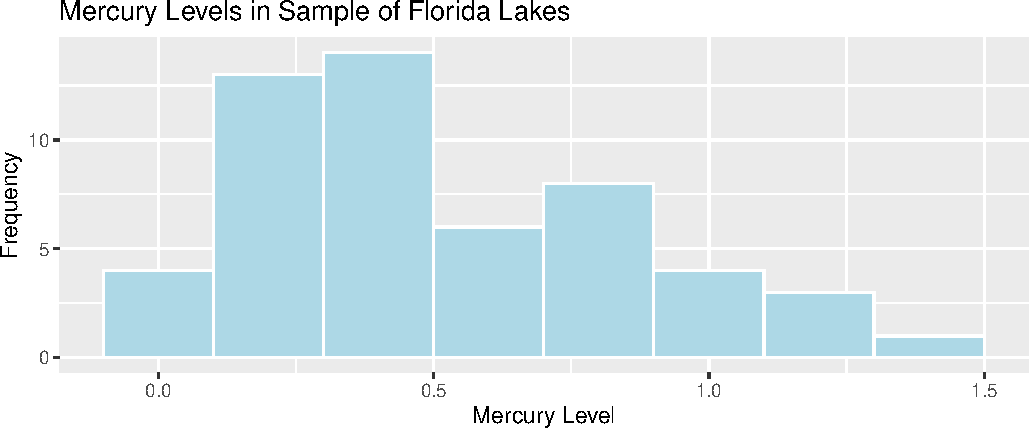
\includegraphics{Ch3_files/figure-pdf/unnamed-chunk-61-1.pdf}

We'll calculate the mean and median mercury level for the 53 lakes in
the sample.

\begin{Shaded}
\begin{Highlighting}[]
\NormalTok{Lakes\_Stats }\OtherTok{\textless{}{-}}\NormalTok{ FloridaLakes }\SpecialCharTok{\%\textgreater{}\%} \FunctionTok{summarize}\NormalTok{(}\AttributeTok{MeanHg =} \FunctionTok{mean}\NormalTok{(Mercury), }
                           \AttributeTok{StDevHG =} \FunctionTok{sd}\NormalTok{(Mercury),}
                           \AttributeTok{N=}\FunctionTok{n}\NormalTok{())}
\FunctionTok{kable}\NormalTok{(Lakes\_Stats)}
\end{Highlighting}
\end{Shaded}

\begin{longtable}[]{@{}rrr@{}}
\toprule\noalign{}
MeanHg & StDevHG & N \\
\midrule\noalign{}
\endhead
\bottomrule\noalign{}
\endlastfoot
0.5271698 & 0.3410356 & 53 \\
\end{longtable}

We want to calculate a 95\% confidence interval for the mean mercury
level among all Florida lakes. We'll use bootstrapping again, this time
using the sample mean, rather than the proportion exceeding 1 ppm, as
our statistic of interest.

\textbf{Bootstrap Steps}

\begin{enumerate}
\def\labelenumi{\arabic{enumi}.}
\item
  Take a sample of 53 lakes by randomly sampling from the original
  sample of 53 lakes, with replacement.
\item
  Calculate the mean mercury level in the bootstrap sample.
\item
  Repeat steps 1 and 2 many (say 10,000) times, keeping track of the
  mean mercury level in each bootstrap sample.
\item
  Look at the distribution of the mean across bootstrap samples. The
  variability in this bootstrap distribution can be used to approximate
  the variability in the sampling distribution for the mean mercury
  level.
\end{enumerate}

We'll illustrate the procedure on 3 bootstrap samples.

\textbf{Bootstrap Sample 1}

The first 10 lakes in the bootstrap sample are shown below. Notice again
that some lakes occur multiple times, and others not at all.

\begin{Shaded}
\begin{Highlighting}[]
\NormalTok{BootstrapSample1 }\OtherTok{\textless{}{-}} \FunctionTok{sample\_n}\NormalTok{(FloridaLakes, }\DecValTok{53}\NormalTok{, }\AttributeTok{replace=}\ConstantTok{TRUE}\NormalTok{) }\SpecialCharTok{\%\textgreater{}\%} \FunctionTok{arrange}\NormalTok{(Lake)}
\NormalTok{BootstrapSample1 }\SpecialCharTok{\%\textgreater{}\%} \FunctionTok{select}\NormalTok{(ID, Lake, Mercury)}
\end{Highlighting}
\end{Shaded}

\begin{verbatim}
# A tibble: 53 x 3
      ID Lake       Mercury
   <int> <chr>        <dbl>
 1     1 Alligator     1.23
 2     2 Annie         1.33
 3     2 Annie         1.33
 4     3 Apopka        0.04
 5     3 Apopka        0.04
 6     3 Apopka        0.04
 7     3 Apopka        0.04
 8     6 Bryant        0.27
 9     9 Deer Point    0.83
10     9 Deer Point    0.83
# i 43 more rows
\end{verbatim}

We calculate the mean mercury level among the lakes in the bootstrap
sample.

\begin{Shaded}
\begin{Highlighting}[]
\FunctionTok{mean}\NormalTok{(BootstrapSample1}\SpecialCharTok{$}\NormalTok{Mercury)}
\end{Highlighting}
\end{Shaded}

\begin{verbatim}
[1] 0.4790566
\end{verbatim}

\textbf{Bootstrap Sample \#2}

\begin{Shaded}
\begin{Highlighting}[]
\NormalTok{BootstrapSample2 }\OtherTok{\textless{}{-}} \FunctionTok{sample\_n}\NormalTok{(FloridaLakes, }\DecValTok{53}\NormalTok{, }\AttributeTok{replace=}\ConstantTok{TRUE}\NormalTok{) }\SpecialCharTok{\%\textgreater{}\%} \FunctionTok{arrange}\NormalTok{(Lake)}
\NormalTok{BootstrapSample2 }\SpecialCharTok{\%\textgreater{}\%} \FunctionTok{select}\NormalTok{(ID, Lake, Mercury)}
\end{Highlighting}
\end{Shaded}

\begin{verbatim}
# A tibble: 53 x 3
      ID Lake       Mercury
   <int> <chr>        <dbl>
 1     1 Alligator     1.23
 2     1 Alligator     1.23
 3     1 Alligator     1.23
 4     2 Annie         1.33
 5     5 Brick         1.2 
 6     6 Bryant        0.27
 7     8 Crescent      0.19
 8     8 Crescent      0.19
 9     9 Deer Point    0.83
10     9 Deer Point    0.83
# i 43 more rows
\end{verbatim}

Mean Mercury Level:

\begin{Shaded}
\begin{Highlighting}[]
\FunctionTok{mean}\NormalTok{(BootstrapSample2}\SpecialCharTok{$}\NormalTok{Mercury)}
\end{Highlighting}
\end{Shaded}

\begin{verbatim}
[1] 0.5479245
\end{verbatim}

\textbf{Bootstrap Sample \#3}

\begin{Shaded}
\begin{Highlighting}[]
\NormalTok{BootstrapSample3 }\OtherTok{\textless{}{-}} \FunctionTok{sample\_n}\NormalTok{(FloridaLakes, }\DecValTok{53}\NormalTok{, }\AttributeTok{replace=}\ConstantTok{TRUE}\NormalTok{) }\SpecialCharTok{\%\textgreater{}\%} \FunctionTok{arrange}\NormalTok{(Lake)}
\NormalTok{BootstrapSample3 }\SpecialCharTok{\%\textgreater{}\%} \FunctionTok{select}\NormalTok{(ID, Lake, Mercury)}
\end{Highlighting}
\end{Shaded}

\begin{verbatim}
# A tibble: 53 x 3
      ID Lake         Mercury
   <int> <chr>          <dbl>
 1     1 Alligator       1.23
 2     3 Apopka          0.04
 3     3 Apopka          0.04
 4     4 Blue Cypress    0.44
 5     5 Brick           1.2 
 6     5 Brick           1.2 
 7     6 Bryant          0.27
 8     7 Cherry          0.48
 9     8 Crescent        0.19
10     9 Deer Point      0.83
# i 43 more rows
\end{verbatim}

Mean Mercury Level:

\begin{Shaded}
\begin{Highlighting}[]
\FunctionTok{mean}\NormalTok{(BootstrapSample3}\SpecialCharTok{$}\NormalTok{Mercury)}
\end{Highlighting}
\end{Shaded}

\begin{verbatim}
[1] 0.5437736
\end{verbatim}

Now, we'll take 10,000 bootstrap samples, and record the mean mercury
concentration in each sample.

\begin{Shaded}
\begin{Highlighting}[]
\NormalTok{mean }\OtherTok{\textless{}{-}} \FunctionTok{mean}\NormalTok{(FloridaLakes}\SpecialCharTok{$}\NormalTok{Mercury)  }\CommentTok{\#calculate sample statistic}
\NormalTok{Bootstrap\_Mean }\OtherTok{\textless{}{-}} \FunctionTok{rep}\NormalTok{(}\ConstantTok{NA}\NormalTok{, }\DecValTok{10000}\NormalTok{) }\CommentTok{\# setup vector to hold bootstrap statistics}

\ControlFlowTok{for}\NormalTok{ (i }\ControlFlowTok{in} \DecValTok{1}\SpecialCharTok{:}\DecValTok{10000}\NormalTok{)\{}
\NormalTok{BootstrapSample }\OtherTok{\textless{}{-}} \FunctionTok{sample\_n}\NormalTok{(FloridaLakes, }\DecValTok{53}\NormalTok{, }\AttributeTok{replace=}\ConstantTok{TRUE}\NormalTok{) }\CommentTok{\# take bootstrap sample}
\NormalTok{Bootstrap\_Mean[i] }\OtherTok{\textless{}{-}} \FunctionTok{mean}\NormalTok{(BootstrapSample}\SpecialCharTok{$}\NormalTok{Mercury) }\CommentTok{\# calculate mean in bootstrap sample}
\NormalTok{\}}
\NormalTok{Lakes\_Bootstrap\_Results\_Mean }\OtherTok{\textless{}{-}} \FunctionTok{data.frame}\NormalTok{(Bootstrap\_Mean)  }\CommentTok{\#store results in data frame}
\end{Highlighting}
\end{Shaded}

The bootstrap distribution for the mean mercury level is shown below,
along with its standard error.

\begin{Shaded}
\begin{Highlighting}[]
\NormalTok{Lakes\_Bootstrap\_Mean\_Plot }\OtherTok{\textless{}{-}} \FunctionTok{ggplot}\NormalTok{(}\AttributeTok{data=}\NormalTok{Lakes\_Bootstrap\_Results\_Mean, }
                                    \FunctionTok{aes}\NormalTok{(}\AttributeTok{x=}\NormalTok{Bootstrap\_Mean)) }\SpecialCharTok{+}  
  \FunctionTok{geom\_histogram}\NormalTok{(}\AttributeTok{color=}\StringTok{"white"}\NormalTok{, }\AttributeTok{fill=}\StringTok{"lightblue"}\NormalTok{) }\SpecialCharTok{+}
  \FunctionTok{xlab}\NormalTok{(}\StringTok{"Mean Mercury in Bootstrap Sample "}\NormalTok{) }\SpecialCharTok{+} \FunctionTok{ylab}\NormalTok{(}\StringTok{"Frequency"}\NormalTok{) }\SpecialCharTok{+}
  \FunctionTok{ggtitle}\NormalTok{(}\StringTok{"Bootstrap Distribution for Sample Mean in Florida Lakes"}\NormalTok{) }\SpecialCharTok{+} 
  \FunctionTok{theme}\NormalTok{(}\AttributeTok{legend.position =} \StringTok{"none"}\NormalTok{) }
\NormalTok{Lakes\_Bootstrap\_Mean\_Plot }
\end{Highlighting}
\end{Shaded}

\includegraphics{Ch3_files/figure-pdf/unnamed-chunk-70-1.pdf}

\textbf{Bootstrap Standard Error}

We'll calculate the bootstrap standard error of the mean. This is a
measure of how much the mean varies between samples of size 53.

\begin{Shaded}
\begin{Highlighting}[]
\NormalTok{SE\_mean }\OtherTok{\textless{}{-}} \FunctionTok{sd}\NormalTok{(Lakes\_Bootstrap\_Results\_Mean}\SpecialCharTok{$}\NormalTok{Bootstrap\_Mean)}
\NormalTok{SE\_mean}
\end{Highlighting}
\end{Shaded}

\begin{verbatim}
[1] 0.04595372
\end{verbatim}

Notice that the standard error of the mean is much less than the sample
standard deviation of 0.341.

\textbf{Interpretations of sample standard deviation and standard error
of the mean}

\begin{itemize}
\item
  The sample standard deviation measures the amount of variability in
  mercury levels between the 53 individual lakes in our sample.
\item
  The standard error of the mean measures the amount of variability in
  sample mean mercury levels between different samples of size 53.
\end{itemize}

There is more variability between mercury levels in individual lakes
than there is between average mercury levels in different samples of
size 53.

Since the bootstrap distribution is roughly symmetric and bell-shaped,
we can use the bootstrap standard error method to calculate an
approximate 95\% confidence interval for the mean mercury level among
all Florida lakes.

\[
\text{Statistic} \pm 2\times\text{Standard Error}
\]

In this case, the statistic of interest is the sample mean
\(\bar{x}=0.527\). The confidence interval is

\[
\begin{aligned}
& \bar{x} \pm 2\times\text{SE}(\bar{x}) \\
& = 0.527 \pm 2\times\text{0.0459537}
\end{aligned}
\]

95\% Confidence Interval:

\begin{Shaded}
\begin{Highlighting}[]
\FunctionTok{c}\NormalTok{(mean }\SpecialCharTok{{-}} \DecValTok{2}\SpecialCharTok{*}\NormalTok{SE\_mean, mean }\SpecialCharTok{+} \DecValTok{2}\SpecialCharTok{*}\NormalTok{SE\_mean) }
\end{Highlighting}
\end{Shaded}

\begin{verbatim}
[1] 0.4352624 0.6190773
\end{verbatim}

The 95\% confidence interval is shown by the gold bar on the graph of
the bootstrap distribution below.

\begin{Shaded}
\begin{Highlighting}[]
\NormalTok{Lakes\_Bootstrap\_Mean\_Plot }\SpecialCharTok{+} 
  \FunctionTok{geom\_segment}\NormalTok{(}\FunctionTok{aes}\NormalTok{(}\AttributeTok{x=}\NormalTok{mean }\SpecialCharTok{{-}} \DecValTok{2}\SpecialCharTok{*}\NormalTok{SE\_mean,}\AttributeTok{xend=}\NormalTok{mean }\SpecialCharTok{+} \DecValTok{2}\SpecialCharTok{*}\NormalTok{SE\_mean, }\AttributeTok{y=}\DecValTok{50}\NormalTok{, }\AttributeTok{yend=}\DecValTok{50}\NormalTok{), }
               \AttributeTok{color=}\StringTok{"gold"}\NormalTok{, }\AttributeTok{size=}\DecValTok{10}\NormalTok{, }\AttributeTok{alpha=}\FloatTok{0.01}\NormalTok{) }
\end{Highlighting}
\end{Shaded}

\includegraphics{Ch3_files/figure-pdf/unnamed-chunk-73-1.pdf}

We are 95\% confident that the average mercury level among all Florida
lakes is between 0.44 and 0.62 parts per million.

It is important to note that we are not saying that we are 95\%
confident that an individual lake lie in this range, or that 95\% of all
individual lakes lie in this range. We are only saying that we are
confident that the \emph{average} mercury level among all lakes lies in
this range. A confidence interval is a statement about a population
parameter (in this case the average mercury level), rather than about
individual lakes in the population. Since there is more variability
about individual lakes than overall averages, we'll need to make a wider
interval when talking about the mercury level for an individual lake.

\subsection{CI for Standard Deviation}\label{ci-for-standard-deviation}

Now, we'll calculate a confidence interval for the standard deviation in
mercury levels among all Florida lakes. Recall that the sample standard
deviation (\(s\)) was:

\begin{Shaded}
\begin{Highlighting}[]
\NormalTok{Sample\_SD }\OtherTok{\textless{}{-}} \FunctionTok{sd}\NormalTok{(FloridaLakes}\SpecialCharTok{$}\NormalTok{Mercury)}
\NormalTok{Sample\_SD}
\end{Highlighting}
\end{Shaded}

\begin{verbatim}
[1] 0.3410356
\end{verbatim}

We'll use this estimate to calculate a confidence interval for the
population standard deviation \(\sigma\).

This time, our statistic of interest is the sample standard deviation
\(s\).

\textbf{Bootstrap Steps}

\begin{enumerate}
\def\labelenumi{\arabic{enumi}.}
\item
  Take a sample of 53 lakes by randomly sampling from the original
  sample of 53 lakes, with replacement.
\item
  Calculate the standard deviation in mercury level in the bootstrap
  sample.
\item
  Repeat steps 1 and 2 many (say 10,000) times, keeping track of the
  standard deviation mercury level in each bootstrap sample.
\item
  Look at the distribution of the standard deviations across bootstrap
  samples. The variability in this bootstrap distribution can be used to
  approximate the variability in the sampling distribution for the
  standard deviation in mercury level.
\end{enumerate}

We'll illustrate the procedure on 3 bootstrap samples.

\textbf{Bootstrap Sample 1}

\begin{Shaded}
\begin{Highlighting}[]
\NormalTok{BootstrapSample1 }\OtherTok{\textless{}{-}} \FunctionTok{sample\_n}\NormalTok{(FloridaLakes, }\DecValTok{53}\NormalTok{, }\AttributeTok{replace=}\ConstantTok{TRUE}\NormalTok{) }\SpecialCharTok{\%\textgreater{}\%} \FunctionTok{arrange}\NormalTok{(Lake)}
\NormalTok{BootstrapSample1 }\SpecialCharTok{\%\textgreater{}\%} \FunctionTok{select}\NormalTok{(ID, Lake, Mercury)}
\end{Highlighting}
\end{Shaded}

\begin{verbatim}
# A tibble: 53 x 3
      ID Lake         Mercury
   <int> <chr>          <dbl>
 1     1 Alligator       1.23
 2     3 Apopka          0.04
 3     4 Blue Cypress    0.44
 4     5 Brick           1.2 
 5     6 Bryant          0.27
 6     6 Bryant          0.27
 7     6 Bryant          0.27
 8     6 Bryant          0.27
 9     7 Cherry          0.48
10     8 Crescent        0.19
# i 43 more rows
\end{verbatim}

We calculate the standard deviation in mercury levels among the lakes in
the bootstrap sample.

\begin{Shaded}
\begin{Highlighting}[]
\FunctionTok{sd}\NormalTok{(BootstrapSample1}\SpecialCharTok{$}\NormalTok{Mercury)}
\end{Highlighting}
\end{Shaded}

\begin{verbatim}
[1] 0.3157289
\end{verbatim}

\textbf{Bootstrap Sample \#2}

\begin{Shaded}
\begin{Highlighting}[]
\NormalTok{BootstrapSample2 }\OtherTok{\textless{}{-}} \FunctionTok{sample\_n}\NormalTok{(FloridaLakes, }\DecValTok{53}\NormalTok{, }\AttributeTok{replace=}\ConstantTok{TRUE}\NormalTok{) }\SpecialCharTok{\%\textgreater{}\%} \FunctionTok{arrange}\NormalTok{(Lake)}
\NormalTok{BootstrapSample2 }\SpecialCharTok{\%\textgreater{}\%} \FunctionTok{select}\NormalTok{(ID, Lake, Mercury)}
\end{Highlighting}
\end{Shaded}

\begin{verbatim}
# A tibble: 53 x 3
      ID Lake         Mercury
   <int> <chr>          <dbl>
 1     1 Alligator       1.23
 2     1 Alligator       1.23
 3     3 Apopka          0.04
 4     4 Blue Cypress    0.44
 5     5 Brick           1.2 
 6     5 Brick           1.2 
 7     6 Bryant          0.27
 8     7 Cherry          0.48
 9     7 Cherry          0.48
10     8 Crescent        0.19
# i 43 more rows
\end{verbatim}

Standard Deviation in Mercury Level:

\begin{Shaded}
\begin{Highlighting}[]
\FunctionTok{sd}\NormalTok{(BootstrapSample2}\SpecialCharTok{$}\NormalTok{Mercury)}
\end{Highlighting}
\end{Shaded}

\begin{verbatim}
[1] 0.3466327
\end{verbatim}

\textbf{Bootstrap Sample \#3}

\begin{Shaded}
\begin{Highlighting}[]
\NormalTok{BootstrapSample3 }\OtherTok{\textless{}{-}} \FunctionTok{sample\_n}\NormalTok{(FloridaLakes, }\DecValTok{53}\NormalTok{, }\AttributeTok{replace=}\ConstantTok{TRUE}\NormalTok{) }\SpecialCharTok{\%\textgreater{}\%} \FunctionTok{arrange}\NormalTok{(Lake)}
\NormalTok{BootstrapSample3 }\SpecialCharTok{\%\textgreater{}\%} \FunctionTok{select}\NormalTok{(ID, Lake, Mercury)}
\end{Highlighting}
\end{Shaded}

\begin{verbatim}
# A tibble: 53 x 3
      ID Lake       Mercury
   <int> <chr>        <dbl>
 1     2 Annie         1.33
 2     3 Apopka        0.04
 3     5 Brick         1.2 
 4     6 Bryant        0.27
 5     6 Bryant        0.27
 6     6 Bryant        0.27
 7     7 Cherry        0.48
 8     8 Crescent      0.19
 9     9 Deer Point    0.83
10     9 Deer Point    0.83
# i 43 more rows
\end{verbatim}

Standard Deviation Mercury Level:

\begin{Shaded}
\begin{Highlighting}[]
\FunctionTok{sd}\NormalTok{(BootstrapSample3}\SpecialCharTok{$}\NormalTok{Mercury)}
\end{Highlighting}
\end{Shaded}

\begin{verbatim}
[1] 0.3294457
\end{verbatim}

Now, we'll take 10,000 bootstrap samples, and record the standard
deviation in mercury concentration in each sample.

\begin{Shaded}
\begin{Highlighting}[]
\NormalTok{Sample\_SD }\OtherTok{\textless{}{-}} \FunctionTok{sd}\NormalTok{(FloridaLakes}\SpecialCharTok{$}\NormalTok{Mercury)  }\CommentTok{\#calculate sample statistic}
\NormalTok{Bootstrap\_SD }\OtherTok{\textless{}{-}} \FunctionTok{rep}\NormalTok{(}\ConstantTok{NA}\NormalTok{, }\DecValTok{10000}\NormalTok{) }\CommentTok{\# setup vector to hold bootstrap statistics}

\ControlFlowTok{for}\NormalTok{ (i }\ControlFlowTok{in} \DecValTok{1}\SpecialCharTok{:}\DecValTok{10000}\NormalTok{)\{}
\NormalTok{BootstrapSample }\OtherTok{\textless{}{-}} \FunctionTok{sample\_n}\NormalTok{(FloridaLakes, }\DecValTok{53}\NormalTok{, }\AttributeTok{replace=}\ConstantTok{TRUE}\NormalTok{) }\CommentTok{\# take bootstrap sample}
\NormalTok{Bootstrap\_SD[i] }\OtherTok{\textless{}{-}} \FunctionTok{sd}\NormalTok{(BootstrapSample}\SpecialCharTok{$}\NormalTok{Mercury) }\CommentTok{\# calculate standard deviation in bootstrap sample}
\NormalTok{\}}
\NormalTok{Lakes\_Bootstrap\_Results\_SD }\OtherTok{\textless{}{-}} \FunctionTok{data.frame}\NormalTok{(Bootstrap\_SD)  }\CommentTok{\#store results in data frame}
\end{Highlighting}
\end{Shaded}

The bootstrap distribution for the mean mercury level is shown below,
along with its standard error.

\begin{Shaded}
\begin{Highlighting}[]
\NormalTok{Lakes\_Bootstrap\_SD\_Plot }\OtherTok{\textless{}{-}} \FunctionTok{ggplot}\NormalTok{(}\AttributeTok{data=}\NormalTok{Lakes\_Bootstrap\_Results\_SD, }
                                    \FunctionTok{aes}\NormalTok{(}\AttributeTok{x=}\NormalTok{Bootstrap\_SD)) }\SpecialCharTok{+}  
  \FunctionTok{geom\_histogram}\NormalTok{(}\AttributeTok{color=}\StringTok{"white"}\NormalTok{, }\AttributeTok{fill=}\StringTok{"lightblue"}\NormalTok{) }\SpecialCharTok{+}
  \FunctionTok{xlab}\NormalTok{(}\StringTok{"SD in Mercury in Bootstrap Sample "}\NormalTok{) }\SpecialCharTok{+} \FunctionTok{ylab}\NormalTok{(}\StringTok{"Frequency"}\NormalTok{) }\SpecialCharTok{+}
  \FunctionTok{ggtitle}\NormalTok{(}\StringTok{"Bootstrap Distribution for Sample SD in Florida Lakes"}\NormalTok{) }\SpecialCharTok{+} 
  \FunctionTok{theme}\NormalTok{(}\AttributeTok{legend.position =} \StringTok{"none"}\NormalTok{) }
\NormalTok{Lakes\_Bootstrap\_SD\_Plot }
\end{Highlighting}
\end{Shaded}

\includegraphics{Ch3_files/figure-pdf/unnamed-chunk-82-1.pdf}

\textbf{Bootstrap Standard Error:}

We'll calculate the bootstrap standard error of the standard deviation.
This is a measure of how much the standard deviation varies between
samples.

\begin{Shaded}
\begin{Highlighting}[]
\NormalTok{SE\_SD }\OtherTok{\textless{}{-}} \FunctionTok{sd}\NormalTok{(Lakes\_Bootstrap\_Results\_SD}\SpecialCharTok{$}\NormalTok{Bootstrap\_SD)}
\NormalTok{SE\_SD}
\end{Highlighting}
\end{Shaded}

\begin{verbatim}
[1] 0.02867548
\end{verbatim}

Since the bootstrap distribution is roughly symmetric and bell-shaped,
we can use the bootstrap standard error method to calculate an
approximate 95\% confidence interval for the standard deviation in
mercury levels among all Florida lakes.

\[
\text{Statistic} \pm 2\times\text{Standard Error}
\]

In this case, the statistic of interest is the sample standard deviation
\(s=0.341\). The confidence interval is

\[
\begin{aligned}
& s \pm 2\times\text{SE}(s) \\
& = 0.341 \pm 2\times{0.029}
\end{aligned}
\]

95\% Confidence Interval:

\begin{Shaded}
\begin{Highlighting}[]
\FunctionTok{c}\NormalTok{(Sample\_SD }\SpecialCharTok{{-}} \DecValTok{2}\SpecialCharTok{*}\NormalTok{SE\_SD, Sample\_SD }\SpecialCharTok{+} \DecValTok{2}\SpecialCharTok{*}\NormalTok{SE\_SD        ) }
\end{Highlighting}
\end{Shaded}

\begin{verbatim}
[1] 0.2836847 0.3983866
\end{verbatim}

The 95\% confidence interval is shown by the gold bar on the graph of
the bootstrap distribution below.

\begin{Shaded}
\begin{Highlighting}[]
\NormalTok{Lakes\_Bootstrap\_SD\_Plot }\SpecialCharTok{+} 
  \FunctionTok{geom\_segment}\NormalTok{(}\FunctionTok{aes}\NormalTok{(}\AttributeTok{x=}\NormalTok{Sample\_SD }\SpecialCharTok{{-}} \DecValTok{2}\SpecialCharTok{*}\NormalTok{SE\_SD,}\AttributeTok{xend=}\NormalTok{Sample\_SD }\SpecialCharTok{+} \DecValTok{2}\SpecialCharTok{*}\NormalTok{SE\_SD, }\AttributeTok{y=}\DecValTok{50}\NormalTok{, }\AttributeTok{yend=}\DecValTok{50}\NormalTok{), }
               \AttributeTok{color=}\StringTok{"gold"}\NormalTok{, }\AttributeTok{size=}\DecValTok{10}\NormalTok{, }\AttributeTok{alpha=}\FloatTok{0.01}\NormalTok{) }
\end{Highlighting}
\end{Shaded}

\includegraphics{Ch3_files/figure-pdf/unnamed-chunk-85-1.pdf}

We are 95\% confident that the standard deviation in mercury levels
among all Florida lakes is between 0.28 and 0.4 parts per million.

\subsection{CI for Median}\label{ci-for-median}

We already calculated a confidence interval for the mean mercury level
among all Florida lakes. We could calculate a bootstrap confidence
interval for the median mercury level as well, but since the
distribution of mercury levels in the lakes is roughly symmetric, the
mean is a reasonable measure of center, and there is not a clear reason
for using the median instead.

When a distribution is skewed or contains large outliers, however, the
median is a more robust measure of center than the mean. Recall the
distribution of 100 Seattle house prices seen in Chapters 1 and 2.

\begin{Shaded}
\begin{Highlighting}[]
\FunctionTok{ggplot}\NormalTok{(}\AttributeTok{data=}\NormalTok{Houses, }\FunctionTok{aes}\NormalTok{(}\AttributeTok{x=}\NormalTok{price)) }\SpecialCharTok{+} 
  \FunctionTok{geom\_histogram}\NormalTok{(}\AttributeTok{fill=}\StringTok{"lightblue"}\NormalTok{, }\AttributeTok{color=}\StringTok{"white"}\NormalTok{) }\SpecialCharTok{+} 
  \FunctionTok{ggtitle}\NormalTok{(}\StringTok{"Distribution of House Prices"}\NormalTok{) }\SpecialCharTok{+}
  \FunctionTok{xlab}\NormalTok{(}\StringTok{"Price"}\NormalTok{) }\SpecialCharTok{+} 
  \FunctionTok{ylab}\NormalTok{(}\StringTok{"Frequency"}\NormalTok{)}
\end{Highlighting}
\end{Shaded}

\includegraphics{Ch3_files/figure-pdf/unnamed-chunk-86-1.pdf}

These 100 houses are a sample of all houses sold in Seattle in 2014 and
2015, so we can use statistics from our sample to draw conclusions about
all houses sold in Seattle in this time period.

In this subsection, we'll use bootstrapping to calculate a 95\%
confidence interval for the median price among all houses sold in
Seattle in this time period.

We calculate the sample median price.

\begin{Shaded}
\begin{Highlighting}[]
\NormalTok{Sample\_Median }\OtherTok{\textless{}{-}} \FunctionTok{median}\NormalTok{(Houses}\SpecialCharTok{$}\NormalTok{price)}
\NormalTok{Sample\_Median}
\end{Highlighting}
\end{Shaded}

\begin{verbatim}
[1] 507.5
\end{verbatim}

\textbf{Bootstrap Steps}

\begin{enumerate}
\def\labelenumi{\arabic{enumi}.}
\item
  Take a sample of 100 houses by randomly sampling from the original
  sample of 100 houses, with replacement.
\item
  Calculate the median price in the bootstrap sample.
\item
  Repeat steps 1 and 2 many (say 10,000) times, keeping track of the
  median price in each bootstrap sample.
\item
  Look at the distribution of the median price across bootstrap samples.
  The variability in this bootstrap distribution can be used to
  approximate the variability in the sampling distribution for the
  median price.
\end{enumerate}

We'll illustrate the procedure on 3 bootstrap samples.

\textbf{Bootstrap Sample 1}

\begin{Shaded}
\begin{Highlighting}[]
\NormalTok{BootstrapSample1 }\OtherTok{\textless{}{-}} \FunctionTok{sample\_n}\NormalTok{(Houses, }\DecValTok{100}\NormalTok{, }\AttributeTok{replace=}\ConstantTok{TRUE}\NormalTok{) }\SpecialCharTok{\%\textgreater{}\%} \FunctionTok{arrange}\NormalTok{(Id)}
\NormalTok{BootstrapSample1 }\SpecialCharTok{\%\textgreater{}\%} \FunctionTok{select}\NormalTok{(Id, price)}
\end{Highlighting}
\end{Shaded}

\begin{verbatim}
# A tibble: 100 x 2
      Id price
   <int> <dbl>
 1     2  885.
 2     3  385.
 3     4  253.
 4     4  253.
 5     5  468.
 6     6  310.
 7     8  485.
 8     9  315.
 9     9  315.
10    10  425 
# i 90 more rows
\end{verbatim}

We calculate the median price among the houses in the bootstrap sample.

\begin{Shaded}
\begin{Highlighting}[]
\FunctionTok{median}\NormalTok{(BootstrapSample1}\SpecialCharTok{$}\NormalTok{price)}
\end{Highlighting}
\end{Shaded}

\begin{verbatim}
[1] 400
\end{verbatim}

\textbf{Bootstrap Sample \#2}

\begin{Shaded}
\begin{Highlighting}[]
\NormalTok{BootstrapSample2 }\OtherTok{\textless{}{-}} \FunctionTok{sample\_n}\NormalTok{(Houses, }\DecValTok{100}\NormalTok{, }\AttributeTok{replace=}\ConstantTok{TRUE}\NormalTok{) }\SpecialCharTok{\%\textgreater{}\%} \FunctionTok{arrange}\NormalTok{(Id)}
\NormalTok{BootstrapSample2 }\SpecialCharTok{\%\textgreater{}\%} \FunctionTok{select}\NormalTok{(Id, price)}
\end{Highlighting}
\end{Shaded}

\begin{verbatim}
# A tibble: 100 x 2
      Id price
   <int> <dbl>
 1     1 1225 
 2     3  385.
 3     4  253.
 4     4  253.
 5     4  253.
 6     6  310.
 7     7  550.
 8     8  485.
 9     8  485.
10     9  315.
# i 90 more rows
\end{verbatim}

Median Price:

\begin{Shaded}
\begin{Highlighting}[]
\FunctionTok{median}\NormalTok{(BootstrapSample2}\SpecialCharTok{$}\NormalTok{price)}
\end{Highlighting}
\end{Shaded}

\begin{verbatim}
[1] 427.5
\end{verbatim}

\textbf{Bootstrap Sample \#3}

\begin{Shaded}
\begin{Highlighting}[]
\NormalTok{BootstrapSample3 }\OtherTok{\textless{}{-}} \FunctionTok{sample\_n}\NormalTok{(Houses, }\DecValTok{100}\NormalTok{, }\AttributeTok{replace=}\ConstantTok{TRUE}\NormalTok{) }\SpecialCharTok{\%\textgreater{}\%} \FunctionTok{arrange}\NormalTok{(Id)}
\NormalTok{BootstrapSample3 }\SpecialCharTok{\%\textgreater{}\%} \FunctionTok{select}\NormalTok{(Id, price)}
\end{Highlighting}
\end{Shaded}

\begin{verbatim}
# A tibble: 100 x 2
      Id price
   <int> <dbl>
 1     2  885.
 2     4  253.
 3     5  468.
 4     7  550.
 5    10  425 
 6    13 1325 
 7    16 3075 
 8    17  438 
 9    18  688.
10    19  995.
# i 90 more rows
\end{verbatim}

Median Price:

\begin{Shaded}
\begin{Highlighting}[]
\FunctionTok{median}\NormalTok{(BootstrapSample3}\SpecialCharTok{$}\NormalTok{price)}
\end{Highlighting}
\end{Shaded}

\begin{verbatim}
[1] 488
\end{verbatim}

Now, we'll take 10,000 bootstrap samples, and record the median price in
each sample.

\begin{Shaded}
\begin{Highlighting}[]
\NormalTok{Sample\_Med }\OtherTok{\textless{}{-}} \FunctionTok{median}\NormalTok{(Houses}\SpecialCharTok{$}\NormalTok{price)  }\CommentTok{\#calculate sample median}
\NormalTok{Bootstrap\_Med }\OtherTok{\textless{}{-}} \FunctionTok{rep}\NormalTok{(}\ConstantTok{NA}\NormalTok{, }\DecValTok{10000}\NormalTok{) }\CommentTok{\# setup vector to hold bootstrap statistics}

\ControlFlowTok{for}\NormalTok{ (i }\ControlFlowTok{in} \DecValTok{1}\SpecialCharTok{:}\DecValTok{10000}\NormalTok{)\{}
\NormalTok{BootstrapSample }\OtherTok{\textless{}{-}} \FunctionTok{sample\_n}\NormalTok{(Houses, }\DecValTok{100}\NormalTok{, }\AttributeTok{replace=}\ConstantTok{TRUE}\NormalTok{) }\CommentTok{\# take bootstrap sample}
\NormalTok{Bootstrap\_Med[i] }\OtherTok{\textless{}{-}} \FunctionTok{median}\NormalTok{(BootstrapSample}\SpecialCharTok{$}\NormalTok{price) }\CommentTok{\# calculate standard deviation in bootstrap sample}
\NormalTok{\}}
\NormalTok{Houses\_Bootstrap\_Results\_Med }\OtherTok{\textless{}{-}} \FunctionTok{data.frame}\NormalTok{(Bootstrap\_Med)  }\CommentTok{\#store results in data frame}
\end{Highlighting}
\end{Shaded}

The bootstrap distribution for the median price is shown below, along
with its standard error.

\begin{Shaded}
\begin{Highlighting}[]
\NormalTok{Houses\_Bootstrap\_Med\_Plot }\OtherTok{\textless{}{-}} \FunctionTok{ggplot}\NormalTok{(}\AttributeTok{data=}\NormalTok{Houses\_Bootstrap\_Results\_Med, }
                                    \FunctionTok{aes}\NormalTok{(}\AttributeTok{x=}\NormalTok{Bootstrap\_Med)) }\SpecialCharTok{+}  
  \FunctionTok{geom\_histogram}\NormalTok{(}\AttributeTok{color=}\StringTok{"white"}\NormalTok{, }\AttributeTok{fill=}\StringTok{"lightblue"}\NormalTok{) }\SpecialCharTok{+}
  \FunctionTok{xlab}\NormalTok{(}\StringTok{"Median Price in Bootstrap Sample "}\NormalTok{) }\SpecialCharTok{+} \FunctionTok{ylab}\NormalTok{(}\StringTok{"Frequency"}\NormalTok{) }\SpecialCharTok{+}
  \FunctionTok{ggtitle}\NormalTok{(}\StringTok{"Bootstrap Distribution for Median Price in Seattle Houses"}\NormalTok{) }\SpecialCharTok{+} 
  \FunctionTok{theme}\NormalTok{(}\AttributeTok{legend.position =} \StringTok{"none"}\NormalTok{) }
\NormalTok{Houses\_Bootstrap\_Med\_Plot }
\end{Highlighting}
\end{Shaded}

\includegraphics{Ch3_files/figure-pdf/unnamed-chunk-95-1.pdf}

\textbf{Bootstrap Standard Error:}

We'll calculate the bootstrap standard error of the median. This is a
measure of how much the median varies between samples.

\begin{Shaded}
\begin{Highlighting}[]
\NormalTok{SE\_Med }\OtherTok{\textless{}{-}} \FunctionTok{sd}\NormalTok{(Houses\_Bootstrap\_Results\_Med}\SpecialCharTok{$}\NormalTok{Bootstrap\_Med)}
\NormalTok{SE\_Med}
\end{Highlighting}
\end{Shaded}

\begin{verbatim}
[1] 48.11411
\end{verbatim}

The standard error measures the amount of variability in median house
price between different samples of size 100.

Note that this is different than the sample standard deviation, which
represents the standard deviation in prices between the 100 different
houses in the sample.

Notice that the bootstrap distribution for the median is not symmetric
and bell-shaped. Thus, we cannot be assured that 95\% of samples will
produce a statistic within two standard errors of the mean, so the
standard error confidence interval method is not appropriate here.
Instead, we'll calculate a confidence interval by taking the middle 95\%
of the values in the bootstrap distribution. A confidence interval
calculated this way is called a \textbf{percentile bootstrap interval}.

We'll calculate the 0.025 quantile and the 0.975 quantile of this
bootstrap distribution. These are the points below which lie 2.5\% and
97.5\% of the medians in the bootstrap distribution. Thus, the middle
95\% of the medians lie between these values.

\begin{Shaded}
\begin{Highlighting}[]
\NormalTok{q}\FloatTok{.025} \OtherTok{\textless{}{-}} \FunctionTok{quantile}\NormalTok{(Houses\_Bootstrap\_Results\_Med}\SpecialCharTok{$}\NormalTok{Bootstrap\_Med, }\FloatTok{0.025}\NormalTok{)}
\NormalTok{q}\FloatTok{.025}
\end{Highlighting}
\end{Shaded}

\begin{verbatim}
2.5% 
 410 
\end{verbatim}

\begin{Shaded}
\begin{Highlighting}[]
\NormalTok{q}\FloatTok{.975} \OtherTok{\textless{}{-}} \FunctionTok{quantile}\NormalTok{(Houses\_Bootstrap\_Results\_Med}\SpecialCharTok{$}\NormalTok{Bootstrap\_Med, }\FloatTok{0.975}\NormalTok{)}
\NormalTok{q}\FloatTok{.975} 
\end{Highlighting}
\end{Shaded}

\begin{verbatim}
 97.5% 
600.05 
\end{verbatim}

The 95\% confidence interval is shown by the gold bar on the graph of
the bootstrap distribution below.

\begin{Shaded}
\begin{Highlighting}[]
\NormalTok{Houses\_Bootstrap\_Med\_Plot }\SpecialCharTok{+} 
  \FunctionTok{geom\_segment}\NormalTok{(}\FunctionTok{aes}\NormalTok{(}\AttributeTok{x=}\NormalTok{q}\FloatTok{.025}\NormalTok{,}\AttributeTok{xend=}\NormalTok{q}\FloatTok{.975}\NormalTok{, }\AttributeTok{y=}\DecValTok{50}\NormalTok{, }\AttributeTok{yend=}\DecValTok{50}\NormalTok{), }
               \AttributeTok{color=}\StringTok{"gold"}\NormalTok{, }\AttributeTok{size=}\DecValTok{10}\NormalTok{, }\AttributeTok{alpha=}\FloatTok{0.01}\NormalTok{) }
\end{Highlighting}
\end{Shaded}

\includegraphics{Ch3_files/figure-pdf/unnamed-chunk-99-1.pdf}

We are 95\% confident that the median price among all houses that sold
in Seattle between 2014 and 2015 is between 410 and 600 thousand
dollars.

\subsection{CI for Difference in
Means}\label{ci-for-difference-in-means}

We previously calculated a confidence interval for the average mercury
level among all lakes in Florida.

Now, we'll calculate an interval for the difference in average mercury
levels between lakes in Northern Florida, compared to Southern Florida.

The boxplot shows and table below describe the distribution of mercury
levels for lakes in Northern Florida, compared to Southern Florida.

\begin{Shaded}
\begin{Highlighting}[]
\NormalTok{LakesBP }\OtherTok{\textless{}{-}} \FunctionTok{ggplot}\NormalTok{(}\AttributeTok{data=}\NormalTok{FloridaLakes, }\FunctionTok{aes}\NormalTok{(}\AttributeTok{x=}\NormalTok{Location, }\AttributeTok{y=}\NormalTok{Mercury, }\AttributeTok{fill=}\NormalTok{Location)) }\SpecialCharTok{+} 
  \FunctionTok{geom\_boxplot}\NormalTok{() }\SpecialCharTok{+}   \FunctionTok{geom\_jitter}\NormalTok{() }\SpecialCharTok{+} \FunctionTok{ggtitle}\NormalTok{(}\StringTok{"Mercury Levels in Florida Lakes"}\NormalTok{) }\SpecialCharTok{+} 
  \FunctionTok{xlab}\NormalTok{(}\StringTok{"Location"}\NormalTok{) }\SpecialCharTok{+} \FunctionTok{ylab}\NormalTok{(}\StringTok{"Mercury Level"}\NormalTok{) }\SpecialCharTok{+} \FunctionTok{theme}\NormalTok{(}\AttributeTok{axis.text.x =} \FunctionTok{element\_text}\NormalTok{(}\AttributeTok{angle =} \DecValTok{90}\NormalTok{)) }\SpecialCharTok{+} \FunctionTok{coord\_flip}\NormalTok{()}
\NormalTok{LakesBP}
\end{Highlighting}
\end{Shaded}

\includegraphics{Ch3_files/figure-pdf/unnamed-chunk-101-1.pdf}

\begin{Shaded}
\begin{Highlighting}[]
\NormalTok{LakesTable }\OtherTok{\textless{}{-}}\NormalTok{ FloridaLakes }\SpecialCharTok{\%\textgreater{}\%} \FunctionTok{group\_by}\NormalTok{(Location) }\SpecialCharTok{\%\textgreater{}\%} \FunctionTok{summarize}\NormalTok{(}\AttributeTok{MeanHg=}\FunctionTok{mean}\NormalTok{(Mercury), }
                                                  \AttributeTok{StDevHg=}\FunctionTok{sd}\NormalTok{(Mercury), }
                                                  \AttributeTok{N=}\FunctionTok{n}\NormalTok{())}
\NormalTok{LakesTable}
\end{Highlighting}
\end{Shaded}

\begin{verbatim}
# A tibble: 2 x 4
  Location MeanHg StDevHg     N
  <fct>     <dbl>   <dbl> <int>
1 N         0.425   0.270    33
2 S         0.696   0.384    20
\end{verbatim}

In our sample of 33 Northern Lakes and 20 Southern Lakes, we saw a
difference of 0.27 ppm. We'll calculate a confidence interval to
estimate how big or small this difference could be among all Florida
lakes.

We'll use a statistical model to calculate the average mercury levels in
Northern and Southern Florida.

\(\widehat{\text{Mercury}} = b_0 +b_1\times{\text{South}}\)

\begin{itemize}
\tightlist
\item
  \(b_0\) represents the mean mercury level for lakes in North Florida,
  and\\
\item
  \(b_1\) represents the mean difference in mercury level for lakes in
  South Florida, compared to North Florida
\end{itemize}

The estimates for corresponding to the original sample are shown below.

\begin{Shaded}
\begin{Highlighting}[]
\NormalTok{M }\OtherTok{\textless{}{-}} \FunctionTok{lm}\NormalTok{(}\AttributeTok{data=}\NormalTok{FloridaLakes, Mercury}\SpecialCharTok{\textasciitilde{}}\NormalTok{Location)}
\NormalTok{M}
\end{Highlighting}
\end{Shaded}

\begin{verbatim}

Call:
lm(formula = Mercury ~ Location, data = FloridaLakes)

Coefficients:
(Intercept)    LocationS  
     0.4245       0.2720  
\end{verbatim}

Thus, we can obtain a confidence interval for the difference in average
mercury levels by fitting a regression model to each of our bootstrap
samples and recording the value of the sample statistic \(b_1\), which
represents this difference. Alternatively, we could calculate the mean
from each group separately and subtract.

When comparing groups, we make one modification in Step \#1 of the
bootstrap process. Rather than drawing a sample of size \(n\) at random,
with replacement, we'll draw the same number of observations from each
group as were in the original sample. In this case, we had 33 northern
lakes, and 20 southern lakes.

\textbf{Bootstrap Steps}

\begin{enumerate}
\def\labelenumi{\arabic{enumi}.}
\item
  Take a sample of 33 northern lakes and 20 southern lakes by randomly
  sampling from the original sample, with replacement.
\item
  Fit a regression model with location as the explanatory variable and
  record the value of \(b_1\), representing the difference between the
  means for each group (South-North).
\item
  Repeat steps 1 and 2 many (say 10,000) times, keeping track of the
  difference in means in each bootstrap sample.
\item
  Look at the distribution of the differences in means across bootstrap
  samples. The variability in this bootstrap distribution can be used to
  approximate the variability in the sampling distribution for the
  difference in means between mercury levels in Northern and Southern
  Florida.
\end{enumerate}

We'll illustrate the procedure on 3 bootstrap samples.

\textbf{Bootstrap Sample 1}

\begin{Shaded}
\begin{Highlighting}[]
\NormalTok{NLakes }\OtherTok{\textless{}{-}} \FunctionTok{sample\_n}\NormalTok{(FloridaLakes }\SpecialCharTok{\%\textgreater{}\%} \FunctionTok{filter}\NormalTok{(Location}\SpecialCharTok{==}\StringTok{"N"}\NormalTok{), }\DecValTok{33}\NormalTok{, }\AttributeTok{replace=}\ConstantTok{TRUE}\NormalTok{)   }\DocumentationTok{\#\# sample 33 northern lakes}
\NormalTok{SLakes }\OtherTok{\textless{}{-}} \FunctionTok{sample\_n}\NormalTok{(FloridaLakes }\SpecialCharTok{\%\textgreater{}\%} \FunctionTok{filter}\NormalTok{(Location}\SpecialCharTok{==}\StringTok{"S"}\NormalTok{), }\DecValTok{20}\NormalTok{, }\AttributeTok{replace=}\ConstantTok{TRUE}\NormalTok{)   }\DocumentationTok{\#\# sample 20 southern lakes}
\NormalTok{BootstrapSample1 }\OtherTok{\textless{}{-}} \FunctionTok{rbind}\NormalTok{(NLakes, SLakes) }\SpecialCharTok{\%\textgreater{}\%} \FunctionTok{arrange}\NormalTok{(ID) }\SpecialCharTok{\%\textgreater{}\%} 
  \FunctionTok{select}\NormalTok{(ID, Lake, Location, Mercury)   }\DocumentationTok{\#\# combine Northern and Southern Lakes}
\NormalTok{BootstrapSample1}
\end{Highlighting}
\end{Shaded}

\begin{verbatim}
# A tibble: 53 x 4
      ID Lake         Location Mercury
   <int> <chr>        <fct>      <dbl>
 1     1 Alligator    S           1.23
 2     2 Annie        S           1.33
 3     2 Annie        S           1.33
 4     3 Apopka       N           0.04
 5     4 Blue Cypress S           0.44
 6     4 Blue Cypress S           0.44
 7     4 Blue Cypress S           0.44
 8     7 Cherry       N           0.48
 9     8 Crescent     N           0.19
10    10 Dias         N           0.81
# i 43 more rows
\end{verbatim}

We fit a regression model to the bootstrap sample and calculate the
regression coefficients. We're interested in the second coefficient,
\(b_1\), which represents the mean difference between lakes in Southern
and Northern Florida

\begin{Shaded}
\begin{Highlighting}[]
\NormalTok{Mb1 }\OtherTok{\textless{}{-}} \FunctionTok{lm}\NormalTok{(}\AttributeTok{data=}\NormalTok{BootstrapSample1, Mercury }\SpecialCharTok{\textasciitilde{}}\NormalTok{ Location) }\DocumentationTok{\#\# fit linear model}
\NormalTok{Mb1}
\end{Highlighting}
\end{Shaded}

\begin{verbatim}

Call:
lm(formula = Mercury ~ Location, data = BootstrapSample1)

Coefficients:
(Intercept)    LocationS  
     0.3894       0.2471  
\end{verbatim}

\begin{Shaded}
\begin{Highlighting}[]
\NormalTok{NLakes }\OtherTok{\textless{}{-}} \FunctionTok{sample\_n}\NormalTok{(FloridaLakes }\SpecialCharTok{\%\textgreater{}\%} \FunctionTok{filter}\NormalTok{(Location}\SpecialCharTok{==}\StringTok{"N"}\NormalTok{), }\DecValTok{33}\NormalTok{, }\AttributeTok{replace=}\ConstantTok{TRUE}\NormalTok{)   }\DocumentationTok{\#\# sample 33 northern lakes}
\NormalTok{SLakes }\OtherTok{\textless{}{-}} \FunctionTok{sample\_n}\NormalTok{(FloridaLakes }\SpecialCharTok{\%\textgreater{}\%} \FunctionTok{filter}\NormalTok{(Location}\SpecialCharTok{==}\StringTok{"S"}\NormalTok{), }\DecValTok{20}\NormalTok{, }\AttributeTok{replace=}\ConstantTok{TRUE}\NormalTok{)   }\DocumentationTok{\#\# sample 20 southern lakes}
\NormalTok{BootstrapSample2 }\OtherTok{\textless{}{-}} \FunctionTok{rbind}\NormalTok{(NLakes, SLakes) }\SpecialCharTok{\%\textgreater{}\%} \FunctionTok{arrange}\NormalTok{(ID) }\SpecialCharTok{\%\textgreater{}\%} 
  \FunctionTok{select}\NormalTok{(ID, Lake, Location, Mercury)   }\DocumentationTok{\#\# combine Northern and Southern Lakes}
\NormalTok{BootstrapSample2}
\end{Highlighting}
\end{Shaded}

\begin{verbatim}
# A tibble: 53 x 4
      ID Lake         Location Mercury
   <int> <chr>        <fct>      <dbl>
 1     1 Alligator    S           1.23
 2     1 Alligator    S           1.23
 3     1 Alligator    S           1.23
 4     1 Alligator    S           1.23
 5     3 Apopka       N           0.04
 6     3 Apopka       N           0.04
 7     3 Apopka       N           0.04
 8     4 Blue Cypress S           0.44
 9     4 Blue Cypress S           0.44
10     4 Blue Cypress S           0.44
# i 43 more rows
\end{verbatim}

\textbf{Bootstrap Sample 2}

\begin{Shaded}
\begin{Highlighting}[]
\NormalTok{Mb2 }\OtherTok{\textless{}{-}} \FunctionTok{lm}\NormalTok{(}\AttributeTok{data=}\NormalTok{BootstrapSample2, Mercury }\SpecialCharTok{\textasciitilde{}}\NormalTok{ Location) }\DocumentationTok{\#\# fit linear model}
\NormalTok{Mb2}
\end{Highlighting}
\end{Shaded}

\begin{verbatim}

Call:
lm(formula = Mercury ~ Location, data = BootstrapSample2)

Coefficients:
(Intercept)    LocationS  
     0.4585       0.2755  
\end{verbatim}

\textbf{Bootstrap Sample 3}

\begin{Shaded}
\begin{Highlighting}[]
\NormalTok{NLakes }\OtherTok{\textless{}{-}} \FunctionTok{sample\_n}\NormalTok{(FloridaLakes }\SpecialCharTok{\%\textgreater{}\%} \FunctionTok{filter}\NormalTok{(Location}\SpecialCharTok{==}\StringTok{"N"}\NormalTok{), }\DecValTok{33}\NormalTok{, }\AttributeTok{replace=}\ConstantTok{TRUE}\NormalTok{)   }\DocumentationTok{\#\# sample 33 northern lakes}
\NormalTok{SLakes }\OtherTok{\textless{}{-}} \FunctionTok{sample\_n}\NormalTok{(FloridaLakes }\SpecialCharTok{\%\textgreater{}\%} \FunctionTok{filter}\NormalTok{(Location}\SpecialCharTok{==}\StringTok{"S"}\NormalTok{), }\DecValTok{20}\NormalTok{, }\AttributeTok{replace=}\ConstantTok{TRUE}\NormalTok{)   }\DocumentationTok{\#\# sample 20 southern lakes}
\NormalTok{BootstrapSample3 }\OtherTok{\textless{}{-}} \FunctionTok{rbind}\NormalTok{(NLakes, SLakes) }\SpecialCharTok{\%\textgreater{}\%} \FunctionTok{arrange}\NormalTok{(ID) }\SpecialCharTok{\%\textgreater{}\%} 
  \FunctionTok{select}\NormalTok{(ID, Lake, Location, Mercury)   }\DocumentationTok{\#\# combine Northern and Southern Lakes}
\NormalTok{BootstrapSample3}
\end{Highlighting}
\end{Shaded}

\begin{verbatim}
# A tibble: 53 x 4
      ID Lake      Location Mercury
   <int> <chr>     <fct>      <dbl>
 1     1 Alligator S           1.23
 2     1 Alligator S           1.23
 3     2 Annie     S           1.33
 4     2 Annie     S           1.33
 5     2 Annie     S           1.33
 6     2 Annie     S           1.33
 7     3 Apopka    N           0.04
 8     3 Apopka    N           0.04
 9     6 Bryant    N           0.27
10     6 Bryant    N           0.27
# i 43 more rows
\end{verbatim}

\begin{Shaded}
\begin{Highlighting}[]
\NormalTok{Mb3 }\OtherTok{\textless{}{-}} \FunctionTok{lm}\NormalTok{(}\AttributeTok{data=}\NormalTok{BootstrapSample3, Mercury }\SpecialCharTok{\textasciitilde{}}\NormalTok{ Location) }\DocumentationTok{\#\# fit linear model}
\NormalTok{Mb3}
\end{Highlighting}
\end{Shaded}

\begin{verbatim}

Call:
lm(formula = Mercury ~ Location, data = BootstrapSample3)

Coefficients:
(Intercept)    LocationS  
     0.3342       0.4178  
\end{verbatim}

We'll now take 10,000 different bootstrap samples and look at the
bootstrap distribution for \(b_1\), the difference in mean mercury
levels between lakes in Southern and Northern Florida

\begin{Shaded}
\begin{Highlighting}[]
\NormalTok{M }\OtherTok{\textless{}{-}} \FunctionTok{lm}\NormalTok{(}\AttributeTok{data=}\NormalTok{FloridaLakes, Mercury}\SpecialCharTok{\textasciitilde{}}\NormalTok{Location) }\CommentTok{\#fit model to original sample}
\NormalTok{Sample\_b1 }\OtherTok{\textless{}{-}}\NormalTok{ M}\SpecialCharTok{$}\NormalTok{coefficients[}\DecValTok{2}\NormalTok{] }\CommentTok{\# record b1 value (second coefficient)}
\NormalTok{Bootstrap\_b1 }\OtherTok{\textless{}{-}} \FunctionTok{rep}\NormalTok{(}\ConstantTok{NA}\NormalTok{, }\DecValTok{10000}\NormalTok{)  }\CommentTok{\#vector to store b1 values}

\ControlFlowTok{for}\NormalTok{ (i }\ControlFlowTok{in} \DecValTok{1}\SpecialCharTok{:}\DecValTok{10000}\NormalTok{)\{}
\NormalTok{NLakes }\OtherTok{\textless{}{-}} \FunctionTok{sample\_n}\NormalTok{(FloridaLakes }\SpecialCharTok{\%\textgreater{}\%} \FunctionTok{filter}\NormalTok{(Location}\SpecialCharTok{==}\StringTok{"N"}\NormalTok{), }\DecValTok{33}\NormalTok{, }\AttributeTok{replace=}\ConstantTok{TRUE}\NormalTok{)   }\DocumentationTok{\#\# sample 33 northern lakes}
\NormalTok{SLakes }\OtherTok{\textless{}{-}} \FunctionTok{sample\_n}\NormalTok{(FloridaLakes }\SpecialCharTok{\%\textgreater{}\%} \FunctionTok{filter}\NormalTok{(Location}\SpecialCharTok{==}\StringTok{"S"}\NormalTok{), }\DecValTok{20}\NormalTok{, }\AttributeTok{replace=}\ConstantTok{TRUE}\NormalTok{)   }\DocumentationTok{\#\# sample 20 southern lakes}
\NormalTok{BootstrapSample }\OtherTok{\textless{}{-}} \FunctionTok{rbind}\NormalTok{(NLakes, SLakes)   }\DocumentationTok{\#\# combine Northern and Southern Lakes}
\NormalTok{M }\OtherTok{\textless{}{-}} \FunctionTok{lm}\NormalTok{(}\AttributeTok{data=}\NormalTok{BootstrapSample, Mercury }\SpecialCharTok{\textasciitilde{}}\NormalTok{ Location) }\DocumentationTok{\#\# fit linear model}
\NormalTok{Bootstrap\_b1[i] }\OtherTok{\textless{}{-}}\NormalTok{ M}\SpecialCharTok{$}\NormalTok{coefficients[}\DecValTok{2}\NormalTok{] }\DocumentationTok{\#\# record b1 }
\NormalTok{\}}
\NormalTok{NS\_Lakes\_Bootstrap\_Results }\OtherTok{\textless{}{-}} \FunctionTok{data.frame}\NormalTok{(Bootstrap\_b1)  }\CommentTok{\#save results as dataframe}
\end{Highlighting}
\end{Shaded}

The bootstrap distribution for the difference in means, \(b_1\), is
shown below, along with the standard error for the difference.

\begin{Shaded}
\begin{Highlighting}[]
\NormalTok{NS\_Lakes\_Bootstrap\_Plot\_b1 }\OtherTok{\textless{}{-}} \FunctionTok{ggplot}\NormalTok{(}\AttributeTok{data=}\NormalTok{NS\_Lakes\_Bootstrap\_Results, }\FunctionTok{aes}\NormalTok{(}\AttributeTok{x=}\NormalTok{Bootstrap\_b1)) }\SpecialCharTok{+}  
  \FunctionTok{geom\_histogram}\NormalTok{(}\AttributeTok{color=}\StringTok{"white"}\NormalTok{, }\AttributeTok{fill=}\StringTok{"lightblue"}\NormalTok{) }\SpecialCharTok{+} 
  \FunctionTok{xlab}\NormalTok{(}\StringTok{"Mean Difference (b1) in Bootstrap Sample"}\NormalTok{) }\SpecialCharTok{+} \FunctionTok{ylab}\NormalTok{(}\StringTok{"Frequency"}\NormalTok{) }\SpecialCharTok{+}
  \FunctionTok{ggtitle}\NormalTok{(}\StringTok{"Northern vs Southern Lakes: Bootstrap Distribution for b1"}\NormalTok{) }
\NormalTok{NS\_Lakes\_Bootstrap\_Plot\_b1}
\end{Highlighting}
\end{Shaded}

\includegraphics{Ch3_files/figure-pdf/unnamed-chunk-111-1.pdf}

\textbf{Bootstrap Standard Error:}

We'll calculate the bootstrap standard error of the difference in means
\(b_1\). This is a measure of how much the difference in means varies
between samples.

\begin{Shaded}
\begin{Highlighting}[]
\NormalTok{SE\_b1 }\OtherTok{\textless{}{-}} \FunctionTok{sd}\NormalTok{(NS\_Lakes\_Bootstrap\_Results}\SpecialCharTok{$}\NormalTok{Bootstrap\_b1)}
\NormalTok{SE\_b1}
\end{Highlighting}
\end{Shaded}

\begin{verbatim}
[1] 0.09549244
\end{verbatim}

The bootstrap distribution is symmetric and bell-shaped, so we can use
the standard error method to calculate a 95\% confidence interval.

\[
\begin{aligned}
& b_1 \pm 2\times\text{SE}(b_1) \\
& = 0.271 \pm 2\times{0.095}
\end{aligned}
\]

95\% Confidence Interval:

\begin{Shaded}
\begin{Highlighting}[]
\FunctionTok{c}\NormalTok{(Sample\_b1 }\SpecialCharTok{{-}} \DecValTok{2}\SpecialCharTok{*}\NormalTok{SE\_b1, Sample\_b1 }\SpecialCharTok{+} \DecValTok{2}\SpecialCharTok{*}\NormalTok{SE\_b1) }
\end{Highlighting}
\end{Shaded}

\begin{verbatim}
 LocationS  LocationS 
0.08096967 0.46293942 
\end{verbatim}

The 95\% confidence interval is shown by the gold bar on the graph of
the bootstrap distribution below.

\begin{Shaded}
\begin{Highlighting}[]
\NormalTok{NS\_Lakes\_Bootstrap\_Plot\_b1 }\SpecialCharTok{+} 
  \FunctionTok{geom\_segment}\NormalTok{(}\FunctionTok{aes}\NormalTok{(}\AttributeTok{x=}\NormalTok{Sample\_b1 }\SpecialCharTok{{-}} \DecValTok{2}\SpecialCharTok{*}\NormalTok{SE\_b1,}\AttributeTok{xend=}\NormalTok{Sample\_b1 }\SpecialCharTok{+} \DecValTok{2}\SpecialCharTok{*}\NormalTok{SE\_b1, }\AttributeTok{y=}\DecValTok{50}\NormalTok{, }\AttributeTok{yend=}\DecValTok{50}\NormalTok{), }
               \AttributeTok{color=}\StringTok{"gold"}\NormalTok{, }\AttributeTok{size=}\DecValTok{10}\NormalTok{, }\AttributeTok{alpha=}\FloatTok{0.01}\NormalTok{) }
\end{Highlighting}
\end{Shaded}

\includegraphics{Ch3_files/figure-pdf/unnamed-chunk-114-1.pdf}

We are 95\% confident that the mean mercury level among all lakes in
Southern Florida is between 0.08 and 0.46 higher than the mean mercury
level among all lakes in Northern Florida.

\subsection{CI for Regression Slope}\label{ci-for-regression-slope}

Now, we'll examine the relationship between mercury concentration and pH
in Florida lakes. The scatterplot displays these variables, along with
the least squares regression line.

\begin{Shaded}
\begin{Highlighting}[]
\FunctionTok{ggplot}\NormalTok{(}\AttributeTok{data=}\NormalTok{FloridaLakes, }\FunctionTok{aes}\NormalTok{(}\AttributeTok{y=}\NormalTok{Mercury, }\AttributeTok{x=}\NormalTok{pH)) }\SpecialCharTok{+} 
  \FunctionTok{geom\_point}\NormalTok{() }\SpecialCharTok{+} \FunctionTok{stat\_smooth}\NormalTok{(}\AttributeTok{method=}\StringTok{"lm"}\NormalTok{, }\AttributeTok{se=}\ConstantTok{FALSE}\NormalTok{)}
\end{Highlighting}
\end{Shaded}

\includegraphics{Ch3_files/figure-pdf/unnamed-chunk-115-1.pdf}

The regression equation is

\[
\widehat{\text{Mercury}} = b_0 + b_1\times\text{pH}
\]

Regression estimates \(b_0\) and \(b_1\) are shown below.

\begin{Shaded}
\begin{Highlighting}[]
\NormalTok{M }\OtherTok{\textless{}{-}} \FunctionTok{lm}\NormalTok{(}\AttributeTok{data=}\NormalTok{FloridaLakes, Mercury}\SpecialCharTok{\textasciitilde{}}\NormalTok{pH)}
\NormalTok{M}
\end{Highlighting}
\end{Shaded}

\begin{verbatim}

Call:
lm(formula = Mercury ~ pH, data = FloridaLakes)

Coefficients:
(Intercept)           pH  
     1.5309      -0.1523  
\end{verbatim}

\begin{itemize}
\tightlist
\item
  On average, lakes with pH level 0 are expected to have a mercury level
  of 1.53 ppm.\\
\item
  For each one-unit increase in pH, mercury level is expected to
  decrease by 0.15 ppm.
\end{itemize}

These estimates are sample statistics, calculated from our sample of 53
lakes. We can think of our regression equation estimates \(b_0\) and
\(b_1\) as estimates of parameters \(\beta_0\) and \(\beta_1\), which
pertain to the slope and intercept of the regression line pertaining to
the entire population of all lakes in Florida. We'll use \(b_0\) and
\(b_1\) to estimate \(\beta_0\) and \(\beta_1\) in the same way that we
used sample proportion \(\hat{p}\) to estimate population proportion
\(p\) and sample mean \(\bar{x}\) to estimate population mean \(\mu\).

The intercept, \(\beta_0\) has little meaning here, but the slope
\(\beta_1\) represents the average change in mercury level for each
one-unit increase in pH, among all Florida lakes. We'll use
bootstrapping to find a confidence interval for this quantity.

\textbf{Bootstrap Steps}

\begin{enumerate}
\def\labelenumi{\arabic{enumi}.}
\item
  Take a sample of 53 lakes by randomly sampling from the original
  sample, with replacement.
\item
  Fit a regression model with pH as the explanatory variable and record
  the value of slope \(b_1\).
\item
  Repeat steps 1 and 2 many (say 10,000) times, keeping track of slope
  of the regression line for each bootstrap sample.
\item
  Look at the distribution of the slopes across bootstrap samples. The
  variability in this bootstrap distribution can be used to approximate
  the variability in the sampling distribution for the slope relating
  mercury and pH levels.
\end{enumerate}

We'll illustrate the procedure on 3 bootstrap samples.

\textbf{Bootstrap Sample 1}

\begin{Shaded}
\begin{Highlighting}[]
\NormalTok{BootstrapSample1 }\OtherTok{\textless{}{-}} \FunctionTok{sample\_n}\NormalTok{(FloridaLakes , }\DecValTok{53}\NormalTok{, }\AttributeTok{replace=}\ConstantTok{TRUE}\NormalTok{)  }\SpecialCharTok{\%\textgreater{}\%} \FunctionTok{arrange}\NormalTok{(ID) }\SpecialCharTok{\%\textgreater{}\%} 
  \FunctionTok{select}\NormalTok{(ID, Lake, pH, Mercury)   }\CommentTok{\# take bootstrap sample}
\NormalTok{BootstrapSample1}
\end{Highlighting}
\end{Shaded}

\begin{verbatim}
# A tibble: 53 x 4
      ID Lake            pH Mercury
   <int> <chr>        <dbl>   <dbl>
 1     1 Alligator      6.1    1.23
 2     1 Alligator      6.1    1.23
 3     2 Annie          5.1    1.33
 4     2 Annie          5.1    1.33
 5     3 Apopka         9.1    0.04
 6     4 Blue Cypress   6.9    0.44
 7     5 Brick          4.6    1.2 
 8     9 Deer Point     5.8    0.83
 9     9 Deer Point     5.8    0.83
10    10 Dias           6.4    0.81
# i 43 more rows
\end{verbatim}

We fit a regression model to the bootstrap sample and calculate the
regression coefficients. We're again interested in the second
coefficient, \(b_1\), which now represents the slope of the regression
line.

\begin{Shaded}
\begin{Highlighting}[]
\NormalTok{Mb1 }\OtherTok{\textless{}{-}} \FunctionTok{lm}\NormalTok{(}\AttributeTok{data=}\NormalTok{BootstrapSample1, Mercury }\SpecialCharTok{\textasciitilde{}}\NormalTok{ pH) }\CommentTok{\# fit linear model}
\NormalTok{Mb1}
\end{Highlighting}
\end{Shaded}

\begin{verbatim}

Call:
lm(formula = Mercury ~ pH, data = BootstrapSample1)

Coefficients:
(Intercept)           pH  
     1.7542      -0.1774  
\end{verbatim}

\textbf{Bootstrap Sample 2}

\begin{Shaded}
\begin{Highlighting}[]
\NormalTok{BootstrapSample2 }\OtherTok{\textless{}{-}} \FunctionTok{sample\_n}\NormalTok{(FloridaLakes , }\DecValTok{53}\NormalTok{, }\AttributeTok{replace=}\ConstantTok{TRUE}\NormalTok{)  }\SpecialCharTok{\%\textgreater{}\%} \FunctionTok{arrange}\NormalTok{(ID) }\SpecialCharTok{\%\textgreater{}\%} 
  \FunctionTok{select}\NormalTok{(ID, Lake, pH, Mercury)}
\NormalTok{BootstrapSample2}
\end{Highlighting}
\end{Shaded}

\begin{verbatim}
# A tibble: 53 x 4
      ID Lake         pH Mercury
   <int> <chr>     <dbl>   <dbl>
 1     1 Alligator   6.1    1.23
 2     2 Annie       5.1    1.33
 3     2 Annie       5.1    1.33
 4     3 Apopka      9.1    0.04
 5     3 Apopka      9.1    0.04
 6     5 Brick       4.6    1.2 
 7     5 Brick       4.6    1.2 
 8     6 Bryant      7.3    0.27
 9     6 Bryant      7.3    0.27
10     7 Cherry      5.4    0.48
# i 43 more rows
\end{verbatim}

\begin{Shaded}
\begin{Highlighting}[]
\NormalTok{Mb2 }\OtherTok{\textless{}{-}} \FunctionTok{lm}\NormalTok{(}\AttributeTok{data=}\NormalTok{BootstrapSample2, Mercury }\SpecialCharTok{\textasciitilde{}}\NormalTok{ pH) }\CommentTok{\# fit linear model}
\NormalTok{Mb2}
\end{Highlighting}
\end{Shaded}

\begin{verbatim}

Call:
lm(formula = Mercury ~ pH, data = BootstrapSample2)

Coefficients:
(Intercept)           pH  
      1.752       -0.189  
\end{verbatim}

\textbf{Bootstrap Sample 3}

\begin{Shaded}
\begin{Highlighting}[]
\NormalTok{BootstrapSample3 }\OtherTok{\textless{}{-}} \FunctionTok{sample\_n}\NormalTok{(FloridaLakes , }\DecValTok{53}\NormalTok{, }\AttributeTok{replace=}\ConstantTok{TRUE}\NormalTok{)  }\SpecialCharTok{\%\textgreater{}\%} \FunctionTok{arrange}\NormalTok{(ID) }\SpecialCharTok{\%\textgreater{}\%} 
  \FunctionTok{select}\NormalTok{(ID, Lake, pH, Mercury)}
\NormalTok{BootstrapSample3}
\end{Highlighting}
\end{Shaded}

\begin{verbatim}
# A tibble: 53 x 4
      ID Lake                 pH Mercury
   <int> <chr>             <dbl>   <dbl>
 1     2 Annie               5.1    1.33
 2     5 Brick               4.6    1.2 
 3     6 Bryant              7.3    0.27
 4     7 Cherry              5.4    0.48
 5    10 Dias                6.4    0.81
 6    11 Dorr                5.4    0.71
 7    14 East Tohopekaliga   5.8    1.16
 8    14 East Tohopekaliga   5.8    1.16
 9    15 Farm-13             7.6    0.05
10    15 Farm-13             7.6    0.05
# i 43 more rows
\end{verbatim}

\begin{Shaded}
\begin{Highlighting}[]
\NormalTok{Mb3 }\OtherTok{\textless{}{-}} \FunctionTok{lm}\NormalTok{(}\AttributeTok{data=}\NormalTok{BootstrapSample3, Mercury }\SpecialCharTok{\textasciitilde{}}\NormalTok{ pH) }\CommentTok{\# fit linear model}
\NormalTok{Mb3}
\end{Highlighting}
\end{Shaded}

\begin{verbatim}

Call:
lm(formula = Mercury ~ pH, data = BootstrapSample3)

Coefficients:
(Intercept)           pH  
     1.2629      -0.1102  
\end{verbatim}

We'll now take 10,000 different bootstrap samples and look at the
bootstrap distribution for \(b_1\), the slope of the regression line
relating mercury level and pH.

\begin{Shaded}
\begin{Highlighting}[]
\NormalTok{M }\OtherTok{\textless{}{-}} \FunctionTok{lm}\NormalTok{(}\AttributeTok{data=}\NormalTok{FloridaLakes, Mercury}\SpecialCharTok{\textasciitilde{}}\NormalTok{pH) }\CommentTok{\#fit model to original sample}
\NormalTok{Sample\_b1 }\OtherTok{\textless{}{-}}\NormalTok{ M}\SpecialCharTok{$}\NormalTok{coefficients[}\DecValTok{2}\NormalTok{] }\CommentTok{\# record b1 value (second coefficient)}
\NormalTok{Bootstrap\_b1 }\OtherTok{\textless{}{-}} \FunctionTok{rep}\NormalTok{(}\ConstantTok{NA}\NormalTok{, }\DecValTok{10000}\NormalTok{)  }\CommentTok{\#vector to store b1 values}

\ControlFlowTok{for}\NormalTok{ (i }\ControlFlowTok{in} \DecValTok{1}\SpecialCharTok{:}\DecValTok{10000}\NormalTok{)\{}
\NormalTok{BootstrapSample }\OtherTok{\textless{}{-}} \FunctionTok{sample\_n}\NormalTok{(FloridaLakes , }\DecValTok{53}\NormalTok{, }\AttributeTok{replace=}\ConstantTok{TRUE}\NormalTok{)   }\CommentTok{\#take bootstrap sample}
\NormalTok{M }\OtherTok{\textless{}{-}} \FunctionTok{lm}\NormalTok{(}\AttributeTok{data=}\NormalTok{BootstrapSample, Mercury }\SpecialCharTok{\textasciitilde{}}\NormalTok{ pH) }\CommentTok{\# fit linear model}
\NormalTok{Bootstrap\_b1[i] }\OtherTok{\textless{}{-}}\NormalTok{ M}\SpecialCharTok{$}\NormalTok{coefficients[}\DecValTok{2}\NormalTok{] }\CommentTok{\# record b1 }
\NormalTok{\}}
\NormalTok{Lakes\_Bootstrap\_Slope\_Results }\OtherTok{\textless{}{-}} \FunctionTok{data.frame}\NormalTok{(Bootstrap\_b1)  }\CommentTok{\#save results as dataframe}
\end{Highlighting}
\end{Shaded}

The bootstrap distribution for the slopes, \(b_1\), is shown below,
along with the standard error for the difference.

\begin{Shaded}
\begin{Highlighting}[]
\NormalTok{Lakes\_Bootstrap\_Plot\_Slope }\OtherTok{\textless{}{-}} \FunctionTok{ggplot}\NormalTok{(}\AttributeTok{data=}\NormalTok{Lakes\_Bootstrap\_Slope\_Results, }\FunctionTok{aes}\NormalTok{(}\AttributeTok{x=}\NormalTok{Bootstrap\_b1)) }\SpecialCharTok{+}
  \FunctionTok{geom\_histogram}\NormalTok{(}\AttributeTok{color=}\StringTok{"white"}\NormalTok{, }\AttributeTok{fill=}\StringTok{"lightblue"}\NormalTok{) }\SpecialCharTok{+} 
  \FunctionTok{xlab}\NormalTok{(}\StringTok{"Slope in Bootstrap Sample"}\NormalTok{) }\SpecialCharTok{+} \FunctionTok{ylab}\NormalTok{(}\StringTok{"Frequency"}\NormalTok{) }\SpecialCharTok{+}
  \FunctionTok{ggtitle}\NormalTok{(}\StringTok{"Bootstrap Distribution for Slope"}\NormalTok{) }
\NormalTok{Lakes\_Bootstrap\_Plot\_Slope}
\end{Highlighting}
\end{Shaded}

\includegraphics{Ch3_files/figure-pdf/unnamed-chunk-124-1.pdf}

\textbf{Bootstrap Standard Error:}

We'll calculate the bootstrap standard error of the slope \(b_1\). This
is a measure of how much the slope varies between samples.

\begin{Shaded}
\begin{Highlighting}[]
\NormalTok{SE\_b1 }\OtherTok{\textless{}{-}} \FunctionTok{sd}\NormalTok{(Lakes\_Bootstrap\_Slope\_Results}\SpecialCharTok{$}\NormalTok{Bootstrap\_b1)}
\NormalTok{SE\_b1}
\end{Highlighting}
\end{Shaded}

\begin{verbatim}
[1] 0.02694529
\end{verbatim}

The bootstrap distribution is symmetric and bell-shaped, so we can use
the standard error method to calculate a 95\% confidence interval.

\[
\begin{aligned}
& b_1 \pm 2\times\text{SE}(b_1) \\
& = -0.1523 \pm 2\times{0.027}
\end{aligned}
\]

95\% Confidence Interval:

\begin{Shaded}
\begin{Highlighting}[]
\FunctionTok{c}\NormalTok{(Sample\_b1 }\SpecialCharTok{{-}} \DecValTok{2}\SpecialCharTok{*}\NormalTok{SE\_b1, Sample\_b1 }\SpecialCharTok{+} \DecValTok{2}\SpecialCharTok{*}\NormalTok{SE\_b1) }
\end{Highlighting}
\end{Shaded}

\begin{verbatim}
         pH          pH 
-0.20619145 -0.09841028 
\end{verbatim}

The 95\% confidence interval is shown by the gold bar on the graph of
the bootstrap distribution below.

\begin{Shaded}
\begin{Highlighting}[]
\NormalTok{Lakes\_Bootstrap\_Plot\_Slope }\SpecialCharTok{+} 
  \FunctionTok{geom\_segment}\NormalTok{(}\FunctionTok{aes}\NormalTok{(}\AttributeTok{x=}\NormalTok{Sample\_b1 }\SpecialCharTok{{-}} \DecValTok{2}\SpecialCharTok{*}\NormalTok{SE\_b1,}\AttributeTok{xend=}\NormalTok{Sample\_b1 }\SpecialCharTok{+} \DecValTok{2}\SpecialCharTok{*}\NormalTok{SE\_b1, }\AttributeTok{y=}\DecValTok{50}\NormalTok{, }\AttributeTok{yend=}\DecValTok{50}\NormalTok{), }
               \AttributeTok{color=}\StringTok{"gold"}\NormalTok{, }\AttributeTok{size=}\DecValTok{10}\NormalTok{, }\AttributeTok{alpha=}\FloatTok{0.01}\NormalTok{) }
\end{Highlighting}
\end{Shaded}

\includegraphics{Ch3_files/figure-pdf/unnamed-chunk-127-1.pdf}

We are 95\% confident that among all Florida lakes, for each 1 unit
increase in pH, mercury level decreases between 0.2 and 0.1, on average.

\subsection{CI for Regression
Response}\label{ci-for-regression-response}

In addition to calculating a confidence interval for the slope of the
regression line relating mercury and pH levels in a lake, we can also
calculate a confidence interval for the average mercury level among all
lakes with a given pH.

We'll calculate a confidence interval for the average mercury level
among all lakes with a neutral pH level of 7.

The regression equation is

\[
\begin{aligned}
\widehat{\text{Mercury}} & = b_0 + b_1\times\text{pH} \\
& = 1.5309 - 0.1523\times\text{pH}
\end{aligned}
\]

so the expected mercury level among all lakes with \(\text{pH} = 7\) is
\(b_0+7b_1 = 1.5309-0.1523(7)=0.4648\) ppm.

This quantity is a statistic calculated from a sample of 53 lakes, so we
would not expect the average mercury level among all lakes in the
population to be exactly equal to 0.4648. Again, we'll use this sample
statistic as an estimate of the population parameter, and use
bootstrapping to estimate the variability associated with this
statistic, in order to make a confidence interval.

\textbf{Bootstrap Steps}

\begin{enumerate}
\def\labelenumi{\arabic{enumi}.}
\item
  Take a sample of 53 lakes by randomly sampling from the original
  sample, with replacement.
\item
  Fit a regression model with location as the explanatory variable and
  record the values of \(b_0\) and \(b_1\). Use these to calculate
  \(b_0+7b_1\).
\item
  Repeat steps 1 and 2 many (say 10,000) times, keeping track of \(b_0\)
  and \(b_1\), and calculating \(b_0+7b_1\) in each bootstrap sample.
\item
  Look at the distribution of the expected response, \(b_0 + 7b_1\),
  across bootstrap samples. The variability in this bootstrap
  distribution can be used to approximate the variability in the
  sampling distribution for the expected mercury level among all lakes
  with pH level of 7.
\end{enumerate}

We'll illustrate the procedure on 3 bootstrap samples.

\textbf{Bootstrap Sample 1}

\begin{Shaded}
\begin{Highlighting}[]
\NormalTok{BootstrapSample1 }\OtherTok{\textless{}{-}} \FunctionTok{sample\_n}\NormalTok{(FloridaLakes , }\DecValTok{53}\NormalTok{, }\AttributeTok{replace=}\ConstantTok{TRUE}\NormalTok{)  }\SpecialCharTok{\%\textgreater{}\%} \FunctionTok{arrange}\NormalTok{(ID) }\SpecialCharTok{\%\textgreater{}\%} 
  \FunctionTok{select}\NormalTok{(ID, Lake, pH, Mercury)   }\CommentTok{\# take bootstrap sample}
\NormalTok{BootstrapSample1}
\end{Highlighting}
\end{Shaded}

\begin{verbatim}
# A tibble: 53 x 4
      ID Lake          pH Mercury
   <int> <chr>      <dbl>   <dbl>
 1     1 Alligator    6.1    1.23
 2     3 Apopka       9.1    0.04
 3     3 Apopka       9.1    0.04
 4     6 Bryant       7.3    0.27
 5     7 Cherry       5.4    0.48
 6     8 Crescent     8.1    0.19
 7     8 Crescent     8.1    0.19
 8     9 Deer Point   5.8    0.83
 9     9 Deer Point   5.8    0.83
10    10 Dias         6.4    0.81
# i 43 more rows
\end{verbatim}

We fit a regression model to the bootstrap sample and calculate the
regression coefficients. We're interested in the second coefficient,
\(b_1\), which represents the mean difference between lakes in Southern
and Northern Florida

\begin{Shaded}
\begin{Highlighting}[]
\NormalTok{Mb1 }\OtherTok{\textless{}{-}} \FunctionTok{lm}\NormalTok{(}\AttributeTok{data=}\NormalTok{BootstrapSample1, Mercury }\SpecialCharTok{\textasciitilde{}}\NormalTok{ pH) }\DocumentationTok{\#\# fit linear model}
\NormalTok{b0 }\OtherTok{\textless{}{-}}\NormalTok{ Mb1}\SpecialCharTok{$}\NormalTok{coefficients[}\DecValTok{1}\NormalTok{] }\CommentTok{\# record value of b0 (first coefficient)}
\NormalTok{b1 }\OtherTok{\textless{}{-}}\NormalTok{ Mb1}\SpecialCharTok{$}\NormalTok{coefficients[}\DecValTok{2}\NormalTok{] }\CommentTok{\# record value of b1 (second coefficient)}
\NormalTok{b0}\SpecialCharTok{+}\DecValTok{7}\SpecialCharTok{*}\NormalTok{b1 }\CommentTok{\#calculate b0+7*b1}
\end{Highlighting}
\end{Shaded}

\begin{verbatim}
(Intercept) 
  0.4353724 
\end{verbatim}

\textbf{Bootstrap Sample 2}

\begin{Shaded}
\begin{Highlighting}[]
\NormalTok{BootstrapSample2 }\OtherTok{\textless{}{-}} \FunctionTok{sample\_n}\NormalTok{(FloridaLakes , }\DecValTok{53}\NormalTok{, }\AttributeTok{replace=}\ConstantTok{TRUE}\NormalTok{)  }\SpecialCharTok{\%\textgreater{}\%} \FunctionTok{arrange}\NormalTok{(ID) }\SpecialCharTok{\%\textgreater{}\%} 
  \FunctionTok{select}\NormalTok{(ID, Lake, pH, Mercury)}
\NormalTok{BootstrapSample2}
\end{Highlighting}
\end{Shaded}

\begin{verbatim}
# A tibble: 53 x 4
      ID Lake            pH Mercury
   <int> <chr>        <dbl>   <dbl>
 1     2 Annie          5.1    1.33
 2     2 Annie          5.1    1.33
 3     3 Apopka         9.1    0.04
 4     4 Blue Cypress   6.9    0.44
 5     6 Bryant         7.3    0.27
 6     6 Bryant         7.3    0.27
 7    10 Dias           6.4    0.81
 8    10 Dias           6.4    0.81
 9    12 Down           7.2    0.5 
10    12 Down           7.2    0.5 
# i 43 more rows
\end{verbatim}

\begin{Shaded}
\begin{Highlighting}[]
\NormalTok{Mb2 }\OtherTok{\textless{}{-}} \FunctionTok{lm}\NormalTok{(}\AttributeTok{data=}\NormalTok{BootstrapSample2, Mercury }\SpecialCharTok{\textasciitilde{}}\NormalTok{ pH) }\CommentTok{\# fit linear model}
\NormalTok{b0 }\OtherTok{\textless{}{-}}\NormalTok{ Mb2}\SpecialCharTok{$}\NormalTok{coefficients[}\DecValTok{1}\NormalTok{] }\CommentTok{\# record value of b0 (first coefficient)}
\NormalTok{b1 }\OtherTok{\textless{}{-}}\NormalTok{ Mb2}\SpecialCharTok{$}\NormalTok{coefficients[}\DecValTok{2}\NormalTok{] }\CommentTok{\# record value of b1 (second coefficient)}
\NormalTok{b0}\SpecialCharTok{+}\DecValTok{7}\SpecialCharTok{*}\NormalTok{b1 }\CommentTok{\#calculate b0+7*b1}
\end{Highlighting}
\end{Shaded}

\begin{verbatim}
(Intercept) 
  0.5738289 
\end{verbatim}

\textbf{Bootstrap Sample 3}

\begin{Shaded}
\begin{Highlighting}[]
\NormalTok{BootstrapSample3 }\OtherTok{\textless{}{-}} \FunctionTok{sample\_n}\NormalTok{(FloridaLakes , }\DecValTok{53}\NormalTok{, }\AttributeTok{replace=}\ConstantTok{TRUE}\NormalTok{)  }\SpecialCharTok{\%\textgreater{}\%} \FunctionTok{arrange}\NormalTok{(ID) }\SpecialCharTok{\%\textgreater{}\%} 
  \FunctionTok{select}\NormalTok{(ID, Lake, pH, Mercury)}
\NormalTok{BootstrapSample3}
\end{Highlighting}
\end{Shaded}

\begin{verbatim}
# A tibble: 53 x 4
      ID Lake        pH Mercury
   <int> <chr>    <dbl>   <dbl>
 1     2 Annie      5.1    1.33
 2     3 Apopka     9.1    0.04
 3     6 Bryant     7.3    0.27
 4     6 Bryant     7.3    0.27
 5     7 Cherry     5.4    0.48
 6     7 Cherry     5.4    0.48
 7     8 Crescent   8.1    0.19
 8    10 Dias       6.4    0.81
 9    10 Dias       6.4    0.81
10    10 Dias       6.4    0.81
# i 43 more rows
\end{verbatim}

\begin{Shaded}
\begin{Highlighting}[]
\NormalTok{Mb3 }\OtherTok{\textless{}{-}} \FunctionTok{lm}\NormalTok{(}\AttributeTok{data=}\NormalTok{BootstrapSample3, Mercury }\SpecialCharTok{\textasciitilde{}}\NormalTok{ pH) }\CommentTok{\# fit linear model}
\NormalTok{b0 }\OtherTok{\textless{}{-}}\NormalTok{ Mb3}\SpecialCharTok{$}\NormalTok{coefficients[}\DecValTok{1}\NormalTok{] }\CommentTok{\# record value of b0 (first coefficient)}
\NormalTok{b1 }\OtherTok{\textless{}{-}}\NormalTok{ Mb3}\SpecialCharTok{$}\NormalTok{coefficients[}\DecValTok{2}\NormalTok{] }\CommentTok{\# record value of b1 (second coefficient)}
\NormalTok{b0}\SpecialCharTok{+}\DecValTok{7}\SpecialCharTok{*}\NormalTok{b1 }\CommentTok{\#calculate b0+7*b1}
\end{Highlighting}
\end{Shaded}

\begin{verbatim}
(Intercept) 
  0.4223812 
\end{verbatim}

We'll now take 10,000 different bootstrap samples and record the values
of \(b_0\), \(b_1\), which we'll then use to calculate \(b_0+7b_1\).

\begin{Shaded}
\begin{Highlighting}[]
\NormalTok{M }\OtherTok{\textless{}{-}} \FunctionTok{lm}\NormalTok{(}\AttributeTok{data=}\NormalTok{FloridaLakes, Mercury}\SpecialCharTok{\textasciitilde{}}\NormalTok{pH) }\CommentTok{\#fit model to original sample}
\NormalTok{Sample\_b0 }\OtherTok{\textless{}{-}}\NormalTok{ M}\SpecialCharTok{$}\NormalTok{coefficients[}\DecValTok{1}\NormalTok{] }\CommentTok{\# record b0 value (second coefficient)}
\NormalTok{Sample\_b1 }\OtherTok{\textless{}{-}}\NormalTok{ M}\SpecialCharTok{$}\NormalTok{coefficients[}\DecValTok{2}\NormalTok{] }\CommentTok{\# record b1 value (second coefficient)}
\NormalTok{Sample\_Exp7 }\OtherTok{\textless{}{-}}\NormalTok{ Sample\_b0 }\SpecialCharTok{+} \DecValTok{7}\SpecialCharTok{*}\NormalTok{Sample\_b1 }\CommentTok{\# calculate sample expected mercury when pH=7}
\NormalTok{Bootstrap\_b0 }\OtherTok{\textless{}{-}} \FunctionTok{rep}\NormalTok{(}\ConstantTok{NA}\NormalTok{, }\DecValTok{10000}\NormalTok{)  }\CommentTok{\#vector to store b1 values}
\NormalTok{Bootstrap\_b1 }\OtherTok{\textless{}{-}} \FunctionTok{rep}\NormalTok{(}\ConstantTok{NA}\NormalTok{, }\DecValTok{10000}\NormalTok{)  }\CommentTok{\#vector to store b1 values}

\ControlFlowTok{for}\NormalTok{ (i }\ControlFlowTok{in} \DecValTok{1}\SpecialCharTok{:}\DecValTok{10000}\NormalTok{)\{}
\NormalTok{BootstrapSample }\OtherTok{\textless{}{-}} \FunctionTok{sample\_n}\NormalTok{(FloridaLakes , }\DecValTok{53}\NormalTok{, }\AttributeTok{replace=}\ConstantTok{TRUE}\NormalTok{)   }\CommentTok{\#take bootstrap sample}
\NormalTok{M }\OtherTok{\textless{}{-}} \FunctionTok{lm}\NormalTok{(}\AttributeTok{data=}\NormalTok{BootstrapSample, Mercury }\SpecialCharTok{\textasciitilde{}}\NormalTok{ pH) }\CommentTok{\# fit linear model}
\NormalTok{Bootstrap\_b0[i] }\OtherTok{\textless{}{-}}\NormalTok{ M}\SpecialCharTok{$}\NormalTok{coefficients[}\DecValTok{1}\NormalTok{] }\CommentTok{\# record b0 }
\NormalTok{Bootstrap\_b1[i] }\OtherTok{\textless{}{-}}\NormalTok{ M}\SpecialCharTok{$}\NormalTok{coefficients[}\DecValTok{2}\NormalTok{] }\CommentTok{\# record b1 }
\NormalTok{\}}

\NormalTok{Bootstrap\_Exp7 }\OtherTok{\textless{}{-}}\NormalTok{  Bootstrap\_b0 }\SpecialCharTok{+} \DecValTok{7}\SpecialCharTok{*}\NormalTok{Bootstrap\_b1 }\CommentTok{\# calcualte expected response for each bootstrap sample}

\NormalTok{Lakes\_Bootstrap\_Exp7\_Results }\OtherTok{\textless{}{-}} \FunctionTok{data.frame}\NormalTok{(Bootstrap\_b0, Bootstrap\_b1, Bootstrap\_Exp7)  }\CommentTok{\#save results as dataframe}
\end{Highlighting}
\end{Shaded}

The bootstrap distribution for the expected mercury level among all
lakes with pH level 7, \(b_0+7b_1\), is shown below, along with the
standard error for this quantity.

\begin{Shaded}
\begin{Highlighting}[]
\NormalTok{Lakes\_Bootstrap\_Plot\_Exp7 }\OtherTok{\textless{}{-}} \FunctionTok{ggplot}\NormalTok{(}\AttributeTok{data=}\NormalTok{Lakes\_Bootstrap\_Exp7\_Results, }\FunctionTok{aes}\NormalTok{(}\AttributeTok{x=}\NormalTok{Bootstrap\_Exp7)) }\SpecialCharTok{+}  
  \FunctionTok{geom\_histogram}\NormalTok{(}\AttributeTok{color=}\StringTok{"white"}\NormalTok{, }\AttributeTok{fill=}\StringTok{"lightblue"}\NormalTok{) }\SpecialCharTok{+} 
  \FunctionTok{xlab}\NormalTok{(}\StringTok{"Expected Mercury Level in Bootstrap Sample"}\NormalTok{) }\SpecialCharTok{+} \FunctionTok{ylab}\NormalTok{(}\StringTok{"Frequency"}\NormalTok{) }\SpecialCharTok{+}
  \FunctionTok{ggtitle}\NormalTok{( }\StringTok{"Bootstrap Distribution for Exp. Mercury when pH=7"}\NormalTok{) }
\NormalTok{Lakes\_Bootstrap\_Plot\_Exp7}
\end{Highlighting}
\end{Shaded}

\includegraphics{Ch3_files/figure-pdf/unnamed-chunk-135-1.pdf}

\textbf{Bootstrap Standard Error:}

We'll calculate the bootstrap standard error of expected mercury
concentration \(b_0 + 7b_1\). This is a measure of how much the
estimated expected concentration varies between samples.

\begin{Shaded}
\begin{Highlighting}[]
\NormalTok{SE\_Exp7 }\OtherTok{\textless{}{-}} \FunctionTok{sd}\NormalTok{(Lakes\_Bootstrap\_Exp7\_Results}\SpecialCharTok{$}\NormalTok{Bootstrap\_Exp7)}
\NormalTok{SE\_Exp7}
\end{Highlighting}
\end{Shaded}

\begin{verbatim}
[1] 0.03702503
\end{verbatim}

Again, the bootstrap distribution is symmetric and bell-shaped, so we
can use the standard error method to calculate a 95\% confidence
interval.

\[
\begin{aligned}
& b_1 \pm 2\times\text{SE}(b_1) \\
& = 0.4648 \pm 2\times{0.037}
\end{aligned}
\]

95\% Confidence Interval:

\begin{Shaded}
\begin{Highlighting}[]
\FunctionTok{c}\NormalTok{(Sample\_Exp7 }\SpecialCharTok{{-}} \DecValTok{2}\SpecialCharTok{*}\NormalTok{SE\_Exp7, Sample\_Exp7 }\SpecialCharTok{+} \DecValTok{2}\SpecialCharTok{*}\NormalTok{SE\_Exp7) }
\end{Highlighting}
\end{Shaded}

\begin{verbatim}
(Intercept) (Intercept) 
  0.3907626   0.5388627 
\end{verbatim}

The 95\% confidence interval is shown by the gold bar on the graph of
the bootstrap distribution below.

\begin{Shaded}
\begin{Highlighting}[]
\NormalTok{Lakes\_Bootstrap\_Plot\_Exp7 }\SpecialCharTok{+} 
  \FunctionTok{geom\_segment}\NormalTok{(}\FunctionTok{aes}\NormalTok{(}\AttributeTok{x=}\NormalTok{Sample\_Exp7 }\SpecialCharTok{{-}} \DecValTok{2}\SpecialCharTok{*}\NormalTok{SE\_Exp7,}\AttributeTok{xend=}\NormalTok{Sample\_Exp7 }\SpecialCharTok{+} \DecValTok{2}\SpecialCharTok{*}\NormalTok{SE\_Exp7, }\AttributeTok{y=}\DecValTok{50}\NormalTok{, }\AttributeTok{yend=}\DecValTok{50}\NormalTok{), }
               \AttributeTok{color=}\StringTok{"gold"}\NormalTok{, }\AttributeTok{size=}\DecValTok{10}\NormalTok{, }\AttributeTok{alpha=}\FloatTok{0.01}\NormalTok{) }
\end{Highlighting}
\end{Shaded}

\includegraphics{Ch3_files/figure-pdf/unnamed-chunk-138-1.pdf}

We are 95\% confident that average mercury level among all Florida lakes
with pH level 7 is between 0.4 and 0.5 ppm.

Again, we are not saying that we think an individual like with a pH
level of 7 will lie in this range, only that the average mercury level
among all such lakes lies in this range.

\subsection{More CI's in Regression}\label{more-cis-in-regression}

We saw in the previous two examples how to calculate a confidence
interval for the slope of a regression line, and for an expected
response in regression. In fact, we can calculate confidence intervals
for any function involving regression coefficients
\(\beta_0, \beta_1, \ldots, \beta_p\), in a similar manner.

For example, let's consider the model for Seattle house prices that
involved square feet, whether or not the house was on the waterfront,
and an interaction term between these variables.

The model is

\[
\widehat{Price} = b_0 + b_1\times\text{Sq. Ft.} + b_2\times\text{waterfront} + b_3\times\text{Sq.Ft}\times\text{Waterfront}
\]

We fit the model and obtain the parameter estimates shown below.

\begin{Shaded}
\begin{Highlighting}[]
\NormalTok{M }\OtherTok{\textless{}{-}} \FunctionTok{lm}\NormalTok{(}\AttributeTok{data=}\NormalTok{Houses, price}\SpecialCharTok{\textasciitilde{}}\NormalTok{sqft\_living }\SpecialCharTok{+}\NormalTok{ waterfront }\SpecialCharTok{+}
\NormalTok{          sqft\_living}\SpecialCharTok{:}\NormalTok{waterfront) }\CommentTok{\#fit model to original sample}
\NormalTok{Sample\_b0 }\OtherTok{\textless{}{-}}\NormalTok{ M}\SpecialCharTok{$}\NormalTok{coefficients[}\DecValTok{1}\NormalTok{] }\CommentTok{\# record b0 value (second coefficient)}
\NormalTok{Sample\_b1 }\OtherTok{\textless{}{-}}\NormalTok{ M}\SpecialCharTok{$}\NormalTok{coefficients[}\DecValTok{2}\NormalTok{] }\CommentTok{\# record b1 value (second coefficient)}
\NormalTok{Sample\_b2 }\OtherTok{\textless{}{-}}\NormalTok{ M}\SpecialCharTok{$}\NormalTok{coefficients[}\DecValTok{3}\NormalTok{] }\CommentTok{\# record b1 value (second coefficient)}
\NormalTok{Sample\_b3 }\OtherTok{\textless{}{-}}\NormalTok{ M}\SpecialCharTok{$}\NormalTok{coefficients[}\DecValTok{4}\NormalTok{] }\CommentTok{\# record b1 value (second coefficient)}
\NormalTok{M}
\end{Highlighting}
\end{Shaded}

\begin{verbatim}

Call:
lm(formula = price ~ sqft_living + waterfront + sqft_living:waterfront, 
    data = Houses)

Coefficients:
              (Intercept)                sqft_living  
                  67.3959                     0.2184  
            waterfrontYes  sqft_living:waterfrontYes  
                -364.5950                     0.4327  
\end{verbatim}

Consider the following quantities that we might be interested in
estimating:

\begin{enumerate}
\def\labelenumi{\arabic{enumi}.}
\tightlist
\item
  The expected price of a 2,000 square foot waterfront house.\\
\item
  The expected price of a 1,500 square foot non-waterfront house.\\
\item
  The difference between the expected price of a house 1,800 square foot
  house on the waterfront, compared to a house the same size that is not
  on the waterfront.\\
\item
  The difference in the rate of change in house prices for each
  additional 100 square feet for houses on the waterfront, compared to
  houses not on the waterfront.
\end{enumerate}

Each of these quantities can be expressed as a linear function of our
regression coefficients \(b_0, b_1, b_2, b_3\). We just need to find the
appropriate function of the \(b_j\)'s, and then calculate a bootstrap
confidence interval for that quantity, using the same steps we've seen
in the previous examples.

Substituting into the regression equation, we see that:

\begin{enumerate}
\def\labelenumi{\arabic{enumi}.}
\tightlist
\item
  The expected price of a 2,000 square foot waterfront house is given by
  \[b_0 + 2000b_1 + b_2 + 2000b_3\]
\end{enumerate}

We calculate this estimate from the model, based on our sample of 100
houses:

\begin{Shaded}
\begin{Highlighting}[]
\DecValTok{2000}\SpecialCharTok{*}\NormalTok{Sample\_b1 }\SpecialCharTok{+}\NormalTok{Sample\_b2}\SpecialCharTok{+}\DecValTok{2000}\SpecialCharTok{*}\NormalTok{Sample\_b3 }\CommentTok{\# calculate b0+2000b1+b2+2000b3}
\end{Highlighting}
\end{Shaded}

\begin{verbatim}
sqft_living 
   937.4777 
\end{verbatim}

We estimate that the average price of all 2,000 square foot waterfront
houses in Seattle is 937 thousand dollars.

\begin{enumerate}
\def\labelenumi{\arabic{enumi}.}
\setcounter{enumi}{1}
\tightlist
\item
  The expected price of a 1,500 square foot non-waterfront house is
  given by \[b_0 + 1500b_1\]
\end{enumerate}

\begin{Shaded}
\begin{Highlighting}[]
\NormalTok{Sample\_b0 }\SpecialCharTok{+} \DecValTok{1500}\SpecialCharTok{*}\NormalTok{Sample\_b1 }\CommentTok{\# calculate b0+1500b1+}
\end{Highlighting}
\end{Shaded}

\begin{verbatim}
(Intercept) 
   394.9499 
\end{verbatim}

We estimate that the average price of all 1,500 square foot
non-waterfront houses in Seattle is 395 thousand dollars.

\begin{enumerate}
\def\labelenumi{\arabic{enumi}.}
\setcounter{enumi}{2}
\tightlist
\item
  The difference between the expected price of a house 1,800 square foot
  house on the waterfront, compared to a house the same size that is not
  on the waterfront is given by:
\end{enumerate}

\[
\begin{aligned}
& (b_0 + 1800b_1 + b_2 + 1800b_3) - (b_0 + 1800b_1) \\
& = b_2 +1800b_3
\end{aligned}
\]

\begin{Shaded}
\begin{Highlighting}[]
\NormalTok{Sample\_b2}\SpecialCharTok{+}\DecValTok{1800}\SpecialCharTok{*}\NormalTok{Sample\_b3 }\CommentTok{\# calculate b2+1800b3}
\end{Highlighting}
\end{Shaded}

\begin{verbatim}
waterfrontYes 
     414.2058 
\end{verbatim}

We estimate that on average a 1,800 square foot house on the waterfront
will cost 414 thousand dollars more than a 1,800 square foot house not
on the waterfront.

\begin{enumerate}
\def\labelenumi{\arabic{enumi}.}
\setcounter{enumi}{3}
\tightlist
\item
  The difference in the rate of change in house prices for each
  additional 100 square feet for houses on the waterfront, compared to
  houses not on the waterfront.
\end{enumerate}

This question is asking about the difference in slopes of the regression
lines relating price and square feet for houses on the waterfront,
compared to those not on the waterfront.

For houses on the waterfront, the regression equation is

\[ \widehat{Price} = (b_0 + b_2) + (b_1 +b_3)\times\text{Sq. Ft.}, \]

so the slope is \(b_1 + b_3\).

For houses not on the waterfront, the regression equation is

\[ \widehat{Price} = b_0 + b_1 \times\text{Sq. Ft.}, \]

so the slope is \(b_1\).

These slope pertain to the expected change in price for each additional
1 square foot. So, for a 100-square foot increase, the price of a
waterfront house is expected to increase by \(100(b_1+b_3)\), compared
to an increase of \(100b_1\) for a non-waterfront house. Thus, the
difference in the rates of change is \(100b_3\).

\begin{Shaded}
\begin{Highlighting}[]
\DecValTok{100}\SpecialCharTok{*}\NormalTok{Sample\_b3 }\CommentTok{\# calculate 100b3}
\end{Highlighting}
\end{Shaded}

\begin{verbatim}
sqft_living:waterfrontYes 
                 43.26671 
\end{verbatim}

We estimate that the price of waterfront houses increases by 43 thousand
dollars more for each additional 100 square feet than the price of
non-waterfront houses.

These estimates calculated from the sample are statistics, which, like
all the other statistics we've seen are likely to vary from the true
values of the corresponding population parameters, due to variability
between samples. We can use bootstrapping to calculate confidence
intervals for the relevant population parameters, using these sample
statistics (the functions of \(b_j\)'s), just as we've done for the
other statistics we've seen.

\textbf{Bootstrap Steps}

\begin{enumerate}
\def\labelenumi{\arabic{enumi}.}
\item
  Take a sample of 100 houses by randomly sampling from the original
  sample, with replacement.
\item
  Fit a regression model with location as the explanatory variable and
  record the values of regression coefficients \(b_0, b_1, b_2, b_3\).
  Use these to calculate each of the four desired quantities
  (i.e.~\(b_0 + 2000b_1 + b_2 +2000b_3\))
\item
  Repeat steps 1 and 2 many (say 10,000) times, keeping track of the
  regression coefficients and calculating the desired quantities in each
  bootstrap sample.
\item
  Look at the distribution of the quantities of interest, across
  bootstrap samples. The variability in this bootstrap distribution can
  be used to approximate the variability in the sampling distribution
  for each of these quantities.
\end{enumerate}

We'll illustrate the procedure on 3 bootstrap samples.

\textbf{Bootstrap Sample 1}

We take the first bootstrap sample and fit a model with interaction. For
brevity, we won't list out the houses in each of the bootstrap samples,
as the idea should be clear by now. Model coefficients are shown below.

\begin{Shaded}
\begin{Highlighting}[]
\NormalTok{BootstrapSample1 }\OtherTok{\textless{}{-}} \FunctionTok{sample\_n}\NormalTok{(Houses , }\DecValTok{100}\NormalTok{, }\AttributeTok{replace=}\ConstantTok{TRUE}\NormalTok{)  }\SpecialCharTok{\%\textgreater{}\%} \FunctionTok{arrange}\NormalTok{(Id) }\SpecialCharTok{\%\textgreater{}\%} 
  \FunctionTok{select}\NormalTok{(Id, price, sqft\_living, waterfront)   }

\NormalTok{Mb1 }\OtherTok{\textless{}{-}} \FunctionTok{lm}\NormalTok{(}\AttributeTok{data=}\NormalTok{BootstrapSample1, price }\SpecialCharTok{\textasciitilde{}}\NormalTok{ sqft\_living }\SpecialCharTok{+}\NormalTok{ waterfront }\SpecialCharTok{+}\NormalTok{ sqft\_living}\SpecialCharTok{:}\NormalTok{waterfront) }\CommentTok{\# fit linear model with interaction}
\NormalTok{b0 }\OtherTok{\textless{}{-}}\NormalTok{ Mb1}\SpecialCharTok{$}\NormalTok{coefficients[}\DecValTok{1}\NormalTok{] }\CommentTok{\# record value of b0 (first coefficient)}
\NormalTok{b1 }\OtherTok{\textless{}{-}}\NormalTok{ Mb1}\SpecialCharTok{$}\NormalTok{coefficients[}\DecValTok{2}\NormalTok{] }\CommentTok{\# record value of b1 (second coefficient)}
\NormalTok{b2 }\OtherTok{\textless{}{-}}\NormalTok{ Mb1}\SpecialCharTok{$}\NormalTok{coefficients[}\DecValTok{3}\NormalTok{] }\CommentTok{\# record value of b2 (third coefficient)}
\NormalTok{b3 }\OtherTok{\textless{}{-}}\NormalTok{ Mb1}\SpecialCharTok{$}\NormalTok{coefficients[}\DecValTok{4}\NormalTok{] }\CommentTok{\# record value of b3 (fourth coefficient)}
\NormalTok{Mb1}
\end{Highlighting}
\end{Shaded}

\begin{verbatim}

Call:
lm(formula = price ~ sqft_living + waterfront + sqft_living:waterfront, 
    data = BootstrapSample1)

Coefficients:
              (Intercept)                sqft_living  
                  69.4180                     0.2308  
            waterfrontYes  sqft_living:waterfrontYes  
                -444.1795                     0.4229  
\end{verbatim}

We calculate each of the four desired quantities.

\begin{Shaded}
\begin{Highlighting}[]
\NormalTok{b0}\SpecialCharTok{+}\DecValTok{2000}\SpecialCharTok{*}\NormalTok{b1 }\SpecialCharTok{+}\NormalTok{ b2 }\SpecialCharTok{+} \DecValTok{2000}\SpecialCharTok{*}\NormalTok{b3}
\end{Highlighting}
\end{Shaded}

\begin{verbatim}
(Intercept) 
   932.7184 
\end{verbatim}

\begin{Shaded}
\begin{Highlighting}[]
\NormalTok{b0}\SpecialCharTok{+}\DecValTok{1500}\SpecialCharTok{*}\NormalTok{b1}
\end{Highlighting}
\end{Shaded}

\begin{verbatim}
(Intercept) 
   415.6311 
\end{verbatim}

\begin{Shaded}
\begin{Highlighting}[]
\NormalTok{b2}\SpecialCharTok{+}\DecValTok{1800}\SpecialCharTok{*}\NormalTok{b3}
\end{Highlighting}
\end{Shaded}

\begin{verbatim}
waterfrontYes 
     317.0968 
\end{verbatim}

\begin{Shaded}
\begin{Highlighting}[]
\DecValTok{100}\SpecialCharTok{*}\NormalTok{b3}
\end{Highlighting}
\end{Shaded}

\begin{verbatim}
sqft_living:waterfrontYes 
                 42.29312 
\end{verbatim}

\textbf{Bootstrap Sample 2}

\begin{Shaded}
\begin{Highlighting}[]
\NormalTok{BootstrapSample2 }\OtherTok{\textless{}{-}} \FunctionTok{sample\_n}\NormalTok{(Houses , }\DecValTok{100}\NormalTok{, }\AttributeTok{replace=}\ConstantTok{TRUE}\NormalTok{)  }\SpecialCharTok{\%\textgreater{}\%} \FunctionTok{arrange}\NormalTok{(Id) }\SpecialCharTok{\%\textgreater{}\%} 
  \FunctionTok{select}\NormalTok{(Id, price, sqft\_living, waterfront)   }

\NormalTok{Mb2 }\OtherTok{\textless{}{-}} \FunctionTok{lm}\NormalTok{(}\AttributeTok{data=}\NormalTok{BootstrapSample2, price }\SpecialCharTok{\textasciitilde{}}\NormalTok{ sqft\_living }\SpecialCharTok{+}\NormalTok{ waterfront }\SpecialCharTok{+}\NormalTok{ sqft\_living}\SpecialCharTok{:}\NormalTok{waterfront) }\CommentTok{\# fit linear model with interaction}
\NormalTok{b0 }\OtherTok{\textless{}{-}}\NormalTok{ Mb2}\SpecialCharTok{$}\NormalTok{coefficients[}\DecValTok{1}\NormalTok{] }\CommentTok{\# record value of b0 (first coefficient)}
\NormalTok{b1 }\OtherTok{\textless{}{-}}\NormalTok{ Mb2}\SpecialCharTok{$}\NormalTok{coefficients[}\DecValTok{2}\NormalTok{] }\CommentTok{\# record value of b1 (second coefficient)}
\NormalTok{b2 }\OtherTok{\textless{}{-}}\NormalTok{ Mb2}\SpecialCharTok{$}\NormalTok{coefficients[}\DecValTok{3}\NormalTok{] }\CommentTok{\# record value of b2 (third coefficient)}
\NormalTok{b3 }\OtherTok{\textless{}{-}}\NormalTok{ Mb2}\SpecialCharTok{$}\NormalTok{coefficients[}\DecValTok{4}\NormalTok{] }\CommentTok{\# record value of b3 (fourth coefficient)}
\NormalTok{Mb2}
\end{Highlighting}
\end{Shaded}

\begin{verbatim}

Call:
lm(formula = price ~ sqft_living + waterfront + sqft_living:waterfront, 
    data = BootstrapSample2)

Coefficients:
              (Intercept)                sqft_living  
                 118.2805                     0.1840  
            waterfrontYes  sqft_living:waterfrontYes  
                -337.1774                     0.4875  
\end{verbatim}

We calculate each of the four desired quantities.

\begin{Shaded}
\begin{Highlighting}[]
\NormalTok{b0}\SpecialCharTok{+}\DecValTok{2000}\SpecialCharTok{*}\NormalTok{b1 }\SpecialCharTok{+}\NormalTok{ b2 }\SpecialCharTok{+} \DecValTok{2000}\SpecialCharTok{*}\NormalTok{b3}
\end{Highlighting}
\end{Shaded}

\begin{verbatim}
(Intercept) 
    1124.13 
\end{verbatim}

\begin{Shaded}
\begin{Highlighting}[]
\NormalTok{b0}\SpecialCharTok{+}\DecValTok{1500}\SpecialCharTok{*}\NormalTok{b1}
\end{Highlighting}
\end{Shaded}

\begin{verbatim}
(Intercept) 
   394.2376 
\end{verbatim}

\begin{Shaded}
\begin{Highlighting}[]
\NormalTok{b2}\SpecialCharTok{+}\DecValTok{1800}\SpecialCharTok{*}\NormalTok{b3}
\end{Highlighting}
\end{Shaded}

\begin{verbatim}
waterfrontYes 
     540.3978 
\end{verbatim}

\begin{Shaded}
\begin{Highlighting}[]
\DecValTok{100}\SpecialCharTok{*}\NormalTok{b3}
\end{Highlighting}
\end{Shaded}

\begin{verbatim}
sqft_living:waterfrontYes 
                 48.75418 
\end{verbatim}

\textbf{Bootstrap Sample 3}

\begin{Shaded}
\begin{Highlighting}[]
\NormalTok{BootstrapSample3 }\OtherTok{\textless{}{-}} \FunctionTok{sample\_n}\NormalTok{(Houses , }\DecValTok{100}\NormalTok{, }\AttributeTok{replace=}\ConstantTok{TRUE}\NormalTok{)  }\SpecialCharTok{\%\textgreater{}\%} \FunctionTok{arrange}\NormalTok{(Id) }\SpecialCharTok{\%\textgreater{}\%} 
  \FunctionTok{select}\NormalTok{(Id, price, sqft\_living, waterfront)   }

\NormalTok{Mb3 }\OtherTok{\textless{}{-}} \FunctionTok{lm}\NormalTok{(}\AttributeTok{data=}\NormalTok{BootstrapSample3, price }\SpecialCharTok{\textasciitilde{}}\NormalTok{ sqft\_living }\SpecialCharTok{+}\NormalTok{ waterfront }\SpecialCharTok{+}\NormalTok{ sqft\_living}\SpecialCharTok{:}\NormalTok{waterfront) }\CommentTok{\# fit linear model with interaction}
\NormalTok{b0 }\OtherTok{\textless{}{-}}\NormalTok{ Mb3}\SpecialCharTok{$}\NormalTok{coefficients[}\DecValTok{1}\NormalTok{] }\CommentTok{\# record value of b0 (first coefficient)}
\NormalTok{b1 }\OtherTok{\textless{}{-}}\NormalTok{ Mb3}\SpecialCharTok{$}\NormalTok{coefficients[}\DecValTok{2}\NormalTok{] }\CommentTok{\# record value of b1 (second coefficient)}
\NormalTok{b2 }\OtherTok{\textless{}{-}}\NormalTok{ Mb3}\SpecialCharTok{$}\NormalTok{coefficients[}\DecValTok{3}\NormalTok{] }\CommentTok{\# record value of b2 (third coefficient)}
\NormalTok{b3 }\OtherTok{\textless{}{-}}\NormalTok{ Mb3}\SpecialCharTok{$}\NormalTok{coefficients[}\DecValTok{4}\NormalTok{] }\CommentTok{\# record value of b3 (fourth coefficient)}
\NormalTok{Mb3}
\end{Highlighting}
\end{Shaded}

\begin{verbatim}

Call:
lm(formula = price ~ sqft_living + waterfront + sqft_living:waterfront, 
    data = BootstrapSample3)

Coefficients:
              (Intercept)                sqft_living  
                  52.4142                     0.2223  
            waterfrontYes  sqft_living:waterfrontYes  
                -260.6892                     0.3865  
\end{verbatim}

We calculate each of the four desired quantities.

\begin{Shaded}
\begin{Highlighting}[]
\NormalTok{b0}\SpecialCharTok{+}\DecValTok{2000}\SpecialCharTok{*}\NormalTok{b1 }\SpecialCharTok{+}\NormalTok{ b2 }\SpecialCharTok{+} \DecValTok{2000}\SpecialCharTok{*}\NormalTok{b3}
\end{Highlighting}
\end{Shaded}

\begin{verbatim}
(Intercept) 
    1009.22 
\end{verbatim}

\begin{Shaded}
\begin{Highlighting}[]
\NormalTok{b0}\SpecialCharTok{+}\DecValTok{1500}\SpecialCharTok{*}\NormalTok{b1}
\end{Highlighting}
\end{Shaded}

\begin{verbatim}
(Intercept) 
    385.811 
\end{verbatim}

\begin{Shaded}
\begin{Highlighting}[]
\NormalTok{b2}\SpecialCharTok{+}\DecValTok{1800}\SpecialCharTok{*}\NormalTok{b3}
\end{Highlighting}
\end{Shaded}

\begin{verbatim}
waterfrontYes 
     434.9802 
\end{verbatim}

\begin{Shaded}
\begin{Highlighting}[]
\DecValTok{100}\SpecialCharTok{*}\NormalTok{b3}
\end{Highlighting}
\end{Shaded}

\begin{verbatim}
sqft_living:waterfrontYes 
                  38.6483 
\end{verbatim}

We'll now take 10,000 different bootstrap samples and record the values
of \(b_0\), \(b_1\), \(b_3\), and \(b_4\), which we'll then use to
calculate each of our four desired quantities.

\begin{Shaded}
\begin{Highlighting}[]
\NormalTok{M }\OtherTok{\textless{}{-}} \FunctionTok{lm}\NormalTok{(}\AttributeTok{data=}\NormalTok{Houses, price}\SpecialCharTok{\textasciitilde{}}\NormalTok{sqft\_living }\SpecialCharTok{+}\NormalTok{ waterfront }\SpecialCharTok{+}
\NormalTok{          sqft\_living}\SpecialCharTok{:}\NormalTok{waterfront) }\CommentTok{\#fit model to original sample}
\NormalTok{Sample\_b0 }\OtherTok{\textless{}{-}}\NormalTok{ M}\SpecialCharTok{$}\NormalTok{coefficients[}\DecValTok{1}\NormalTok{] }\CommentTok{\# record b0 value (second coefficient)}
\NormalTok{Sample\_b1 }\OtherTok{\textless{}{-}}\NormalTok{ M}\SpecialCharTok{$}\NormalTok{coefficients[}\DecValTok{2}\NormalTok{] }\CommentTok{\# record b1 value (second coefficient)}
\NormalTok{Sample\_b2 }\OtherTok{\textless{}{-}}\NormalTok{ M}\SpecialCharTok{$}\NormalTok{coefficients[}\DecValTok{3}\NormalTok{] }\CommentTok{\# record b1 value (second coefficient)}
\NormalTok{Sample\_b3 }\OtherTok{\textless{}{-}}\NormalTok{ M}\SpecialCharTok{$}\NormalTok{coefficients[}\DecValTok{4}\NormalTok{] }\CommentTok{\# record b1 value (second coefficient)}
\NormalTok{Sample\_Q1 }\OtherTok{\textless{}{-}}\NormalTok{ Sample\_b0 }\SpecialCharTok{+} \DecValTok{2000}\SpecialCharTok{*}\NormalTok{Sample\_b1 }\SpecialCharTok{+}\NormalTok{Sample\_b2}\SpecialCharTok{+}\DecValTok{2000}\SpecialCharTok{*}\NormalTok{Sample\_b3 }\CommentTok{\# calculate b0+2000b1+b2+2000b3}
\NormalTok{Sample\_Q2 }\OtherTok{\textless{}{-}}\NormalTok{ Sample\_b0 }\SpecialCharTok{+} \DecValTok{1500}\SpecialCharTok{*}\NormalTok{Sample\_b1 }\CommentTok{\# calculate b0+1500b1+}
\NormalTok{Sample\_Q3 }\OtherTok{\textless{}{-}}\NormalTok{ Sample\_b2}\SpecialCharTok{+}\DecValTok{1800}\SpecialCharTok{*}\NormalTok{Sample\_b3 }\CommentTok{\# calculate b2+1800b3}
\NormalTok{Sample\_Q4 }\OtherTok{\textless{}{-}} \DecValTok{100}\SpecialCharTok{*}\NormalTok{Sample\_b3 }\CommentTok{\# calculate 100b3}

\NormalTok{Bootstrap\_b0 }\OtherTok{\textless{}{-}} \FunctionTok{rep}\NormalTok{(}\ConstantTok{NA}\NormalTok{, }\DecValTok{10000}\NormalTok{)  }\CommentTok{\#vector to store b0 values}
\NormalTok{Bootstrap\_b1 }\OtherTok{\textless{}{-}} \FunctionTok{rep}\NormalTok{(}\ConstantTok{NA}\NormalTok{, }\DecValTok{10000}\NormalTok{)  }\CommentTok{\#vector to store b1 values}
\NormalTok{Bootstrap\_b2 }\OtherTok{\textless{}{-}} \FunctionTok{rep}\NormalTok{(}\ConstantTok{NA}\NormalTok{, }\DecValTok{10000}\NormalTok{)  }\CommentTok{\#vector to store b2 values}
\NormalTok{Bootstrap\_b3 }\OtherTok{\textless{}{-}} \FunctionTok{rep}\NormalTok{(}\ConstantTok{NA}\NormalTok{, }\DecValTok{10000}\NormalTok{)  }\CommentTok{\#vector to store b3 values}


\ControlFlowTok{for}\NormalTok{ (i }\ControlFlowTok{in} \DecValTok{1}\SpecialCharTok{:}\DecValTok{10000}\NormalTok{)\{}
\NormalTok{BootstrapSample }\OtherTok{\textless{}{-}} \FunctionTok{sample\_n}\NormalTok{(Houses, }\DecValTok{1000}\NormalTok{, }\AttributeTok{replace=}\ConstantTok{TRUE}\NormalTok{)   }\CommentTok{\#take bootstrap sample}
\NormalTok{Mb }\OtherTok{\textless{}{-}} \FunctionTok{lm}\NormalTok{(}\AttributeTok{data=}\NormalTok{BootstrapSample, price }\SpecialCharTok{\textasciitilde{}}\NormalTok{ sqft\_living }\SpecialCharTok{+} 
\NormalTok{           waterfront }\SpecialCharTok{+}\NormalTok{ sqft\_living}\SpecialCharTok{:}\NormalTok{waterfront) }\CommentTok{\# fit linear model with interaction}
\NormalTok{Bootstrap\_b0[i] }\OtherTok{\textless{}{-}}\NormalTok{ Mb}\SpecialCharTok{$}\NormalTok{coefficients[}\DecValTok{1}\NormalTok{] }\CommentTok{\# record value of b0 (first coefficient)}
\NormalTok{Bootstrap\_b1[i] }\OtherTok{\textless{}{-}}\NormalTok{ Mb}\SpecialCharTok{$}\NormalTok{coefficients[}\DecValTok{2}\NormalTok{] }\CommentTok{\# record value of b1 (second coefficient)}
\NormalTok{Bootstrap\_b2[i] }\OtherTok{\textless{}{-}}\NormalTok{ Mb}\SpecialCharTok{$}\NormalTok{coefficients[}\DecValTok{3}\NormalTok{] }\CommentTok{\# record value of b2 (third coefficient)}
\NormalTok{Bootstrap\_b3[i] }\OtherTok{\textless{}{-}}\NormalTok{ Mb}\SpecialCharTok{$}\NormalTok{coefficients[}\DecValTok{4}\NormalTok{] }\CommentTok{\# record value of b3 (fourth coefficient)}
\NormalTok{\}}

\NormalTok{Bootstrap\_Q1 }\OtherTok{\textless{}{-}}\NormalTok{  Bootstrap\_b0 }\SpecialCharTok{+} \DecValTok{2000}\SpecialCharTok{*}\NormalTok{Bootstrap\_b1 }\SpecialCharTok{+}\NormalTok{ Bootstrap\_b2 }\SpecialCharTok{+} \DecValTok{2000}\SpecialCharTok{*}\NormalTok{Bootstrap\_b3}
\NormalTok{Bootstrap\_Q2 }\OtherTok{\textless{}{-}}\NormalTok{  Bootstrap\_b0 }\SpecialCharTok{+} \DecValTok{1500}\SpecialCharTok{*}\NormalTok{Bootstrap\_b1 }
\NormalTok{Bootstrap\_Q3 }\OtherTok{\textless{}{-}}\NormalTok{  Bootstrap\_b2 }\SpecialCharTok{+} \DecValTok{1800}\SpecialCharTok{*}\NormalTok{Bootstrap\_b3}
\NormalTok{Bootstrap\_Q4 }\OtherTok{\textless{}{-}}  \DecValTok{100}\SpecialCharTok{*}\NormalTok{Bootstrap\_b3}

\NormalTok{Houses\_Bootstrap\_Results }\OtherTok{\textless{}{-}} \FunctionTok{data.frame}\NormalTok{(Bootstrap\_b0, Bootstrap\_b1, Bootstrap\_b2, Bootstrap\_b3, Bootstrap\_Q1, Bootstrap\_Q2 , Bootstrap\_Q3 , Bootstrap\_Q4)  }\CommentTok{\#save results as dataframe}
\end{Highlighting}
\end{Shaded}

\textbf{Bootstrap Distribution for} \(b_0 + 2000b_1 + b_2 + 2000b_3\)

\begin{Shaded}
\begin{Highlighting}[]
\NormalTok{Houses\_Bootstrap\_Plot\_Q1 }\OtherTok{\textless{}{-}} \FunctionTok{ggplot}\NormalTok{(}\AttributeTok{data=}\NormalTok{Houses\_Bootstrap\_Results, }
                                   \FunctionTok{aes}\NormalTok{(}\AttributeTok{x=}\NormalTok{Bootstrap\_Q1)) }\SpecialCharTok{+}  
  \FunctionTok{geom\_histogram}\NormalTok{(}\AttributeTok{color=}\StringTok{"white"}\NormalTok{, }\AttributeTok{fill=}\StringTok{"lightblue"}\NormalTok{) }\SpecialCharTok{+} 
  \FunctionTok{xlab}\NormalTok{(}\StringTok{"Expected Price of 2000 Sq. Ft. Waterfront House"}\NormalTok{) }\SpecialCharTok{+} \FunctionTok{ylab}\NormalTok{(}\StringTok{"Frequency"}\NormalTok{) }\SpecialCharTok{+}
  \FunctionTok{ggtitle}\NormalTok{( }\StringTok{"Bootstrap Distribution b0+2000b1+b2+2000b3"}\NormalTok{) }
\NormalTok{Houses\_Bootstrap\_Plot\_Q1}
\end{Highlighting}
\end{Shaded}

\includegraphics{Ch3_files/figure-pdf/unnamed-chunk-160-1.pdf}

Standard Error:

\begin{Shaded}
\begin{Highlighting}[]
\NormalTok{SE\_Q1 }\OtherTok{\textless{}{-}} \FunctionTok{sd}\NormalTok{(Houses\_Bootstrap\_Results}\SpecialCharTok{$}\NormalTok{Bootstrap\_Q1)}
\NormalTok{SE\_Q1}
\end{Highlighting}
\end{Shaded}

\begin{verbatim}
[1] 40.03112
\end{verbatim}

The bootstrap distribution is symmetric and bell-shaped, so we can use
the standard error method to calculate a 95\% confidence interval.

95\% Confidence Interval:

\begin{Shaded}
\begin{Highlighting}[]
\FunctionTok{c}\NormalTok{(Sample\_Q1 }\SpecialCharTok{{-}} \DecValTok{2}\SpecialCharTok{*}\NormalTok{SE\_Q1, Sample\_Q1 }\SpecialCharTok{+} \DecValTok{2}\SpecialCharTok{*}\NormalTok{SE\_Q1) }
\end{Highlighting}
\end{Shaded}

\begin{verbatim}
(Intercept) (Intercept) 
   924.8114   1084.9359 
\end{verbatim}

The 95\% confidence interval is shown by the gold bar on the graph of
the bootstrap distribution below.

\begin{Shaded}
\begin{Highlighting}[]
\NormalTok{Houses\_Bootstrap\_Plot\_Q1 }\SpecialCharTok{+} 
  \FunctionTok{geom\_segment}\NormalTok{(}\FunctionTok{aes}\NormalTok{(}\AttributeTok{x=}\NormalTok{Sample\_Q1 }\SpecialCharTok{{-}} \DecValTok{2}\SpecialCharTok{*}\NormalTok{SE\_Q1,}\AttributeTok{xend=}\NormalTok{Sample\_Q1 }\SpecialCharTok{+} \DecValTok{2}\SpecialCharTok{*}\NormalTok{SE\_Q1, }\AttributeTok{y=}\DecValTok{50}\NormalTok{, }\AttributeTok{yend=}\DecValTok{50}\NormalTok{), }
               \AttributeTok{color=}\StringTok{"gold"}\NormalTok{, }\AttributeTok{size=}\DecValTok{10}\NormalTok{, }\AttributeTok{alpha=}\FloatTok{0.01}\NormalTok{) }
\end{Highlighting}
\end{Shaded}

\includegraphics{Ch3_files/figure-pdf/unnamed-chunk-163-1.pdf}

We are 95\% confident that average price among all 2,000 square foot
Seattle waterfront houses is between 924.8114379 and 1084.9359281
thousand dollars.

\textbf{Bootstrap Distribution for} \(b_0 + 1500b_1\)

\begin{Shaded}
\begin{Highlighting}[]
\NormalTok{Houses\_Bootstrap\_Plot\_Q2 }\OtherTok{\textless{}{-}} \FunctionTok{ggplot}\NormalTok{(}\AttributeTok{data=}\NormalTok{Houses\_Bootstrap\_Results, }
                                   \FunctionTok{aes}\NormalTok{(}\AttributeTok{x=}\NormalTok{Bootstrap\_Q2)) }\SpecialCharTok{+}  
  \FunctionTok{geom\_histogram}\NormalTok{(}\AttributeTok{color=}\StringTok{"white"}\NormalTok{, }\AttributeTok{fill=}\StringTok{"lightblue"}\NormalTok{) }\SpecialCharTok{+} 
  \FunctionTok{xlab}\NormalTok{(}\StringTok{"Expected Price of 1500 Sq. Ft. Non{-}Waterfront House"}\NormalTok{) }\SpecialCharTok{+} \FunctionTok{ylab}\NormalTok{(}\StringTok{"Frequency"}\NormalTok{) }\SpecialCharTok{+}
  \FunctionTok{ggtitle}\NormalTok{( }\StringTok{"Bootstrap Distribution b0+1500b1"}\NormalTok{) }
\NormalTok{Houses\_Bootstrap\_Plot\_Q2}
\end{Highlighting}
\end{Shaded}

\includegraphics{Ch3_files/figure-pdf/unnamed-chunk-164-1.pdf}

Standard Error:

\begin{Shaded}
\begin{Highlighting}[]
\NormalTok{SE\_Q2 }\OtherTok{\textless{}{-}} \FunctionTok{sd}\NormalTok{(Houses\_Bootstrap\_Results}\SpecialCharTok{$}\NormalTok{Bootstrap\_Q2)}
\NormalTok{SE\_Q2}
\end{Highlighting}
\end{Shaded}

\begin{verbatim}
[1] 5.812557
\end{verbatim}

The bootstrap distribution is symmetric and bell-shaped, so we can use
the standard error method to calculate a 95\% confidence interval.

95\% Confidence Interval:

\begin{Shaded}
\begin{Highlighting}[]
\FunctionTok{c}\NormalTok{(Sample\_Q2 }\SpecialCharTok{{-}} \DecValTok{2}\SpecialCharTok{*}\NormalTok{SE\_Q2, Sample\_Q2 }\SpecialCharTok{+} \DecValTok{2}\SpecialCharTok{*}\NormalTok{SE\_Q2) }
\end{Highlighting}
\end{Shaded}

\begin{verbatim}
(Intercept) (Intercept) 
   383.3247    406.5750 
\end{verbatim}

The 95\% confidence interval is shown by the gold bar on the graph of
the bootstrap distribution below.

\begin{Shaded}
\begin{Highlighting}[]
\NormalTok{Houses\_Bootstrap\_Plot\_Q2 }\SpecialCharTok{+} 
  \FunctionTok{geom\_segment}\NormalTok{(}\FunctionTok{aes}\NormalTok{(}\AttributeTok{x=}\NormalTok{Sample\_Q2 }\SpecialCharTok{{-}} \DecValTok{2}\SpecialCharTok{*}\NormalTok{SE\_Q2,}\AttributeTok{xend=}\NormalTok{Sample\_Q2 }\SpecialCharTok{+} \DecValTok{2}\SpecialCharTok{*}\NormalTok{SE\_Q2, }\AttributeTok{y=}\DecValTok{50}\NormalTok{, }\AttributeTok{yend=}\DecValTok{50}\NormalTok{), }
               \AttributeTok{color=}\StringTok{"gold"}\NormalTok{, }\AttributeTok{size=}\DecValTok{10}\NormalTok{, }\AttributeTok{alpha=}\FloatTok{0.01}\NormalTok{) }
\end{Highlighting}
\end{Shaded}

\includegraphics{Ch3_files/figure-pdf/unnamed-chunk-167-1.pdf}

We are 95\% confident that average price among all 1,500 square foot
Seattle non-waterfront houses is between 383.3247413 and 406.5749705
thousand dollars.

\textbf{Bootstrap Distribution for} \(b_2 + 1800b_3\)

\begin{Shaded}
\begin{Highlighting}[]
\NormalTok{Houses\_Bootstrap\_Plot\_Q3 }\OtherTok{\textless{}{-}} \FunctionTok{ggplot}\NormalTok{(}\AttributeTok{data=}\NormalTok{Houses\_Bootstrap\_Results, }
                                   \FunctionTok{aes}\NormalTok{(}\AttributeTok{x=}\NormalTok{Bootstrap\_Q3)) }\SpecialCharTok{+}  
  \FunctionTok{geom\_histogram}\NormalTok{(}\AttributeTok{color=}\StringTok{"white"}\NormalTok{, }\AttributeTok{fill=}\StringTok{"lightblue"}\NormalTok{) }\SpecialCharTok{+} 
  \FunctionTok{xlab}\NormalTok{(}\StringTok{"Expected Price Difference WF vs NWF for 1800 sq. Ft. House"}\NormalTok{) }\SpecialCharTok{+} \FunctionTok{ylab}\NormalTok{(}\StringTok{"Frequency"}\NormalTok{) }\SpecialCharTok{+}
  \FunctionTok{ggtitle}\NormalTok{( }\StringTok{"Bootstrap Distribution b2+1800b3"}\NormalTok{) }
\NormalTok{Houses\_Bootstrap\_Plot\_Q3}
\end{Highlighting}
\end{Shaded}

\includegraphics{Ch3_files/figure-pdf/unnamed-chunk-168-1.pdf}

Standard Error:

\begin{Shaded}
\begin{Highlighting}[]
\NormalTok{SE\_Q3 }\OtherTok{\textless{}{-}} \FunctionTok{sd}\NormalTok{(Houses\_Bootstrap\_Results}\SpecialCharTok{$}\NormalTok{Bootstrap\_Q3)}
\NormalTok{SE\_Q3}
\end{Highlighting}
\end{Shaded}

\begin{verbatim}
[1] 40.38204
\end{verbatim}

The bootstrap distribution is symmetric and bell-shaped, so we can use
the standard error method to calculate a 95\% confidence interval.

95\% Confidence Interval:

\begin{Shaded}
\begin{Highlighting}[]
\FunctionTok{c}\NormalTok{(Sample\_Q3 }\SpecialCharTok{{-}} \DecValTok{2}\SpecialCharTok{*}\NormalTok{SE\_Q3, Sample\_Q3 }\SpecialCharTok{+} \DecValTok{2}\SpecialCharTok{*}\NormalTok{SE\_Q3) }
\end{Highlighting}
\end{Shaded}

\begin{verbatim}
waterfrontYes waterfrontYes 
     333.4417      494.9698 
\end{verbatim}

The 95\% confidence interval is shown by the gold bar on the graph of
the bootstrap distribution below.

\begin{Shaded}
\begin{Highlighting}[]
\NormalTok{Houses\_Bootstrap\_Plot\_Q3 }\SpecialCharTok{+} 
  \FunctionTok{geom\_segment}\NormalTok{(}\FunctionTok{aes}\NormalTok{(}\AttributeTok{x=}\NormalTok{Sample\_Q3 }\SpecialCharTok{{-}} \DecValTok{2}\SpecialCharTok{*}\NormalTok{SE\_Q3,}\AttributeTok{xend=}\NormalTok{Sample\_Q3 }\SpecialCharTok{+} \DecValTok{2}\SpecialCharTok{*}\NormalTok{SE\_Q3, }\AttributeTok{y=}\DecValTok{50}\NormalTok{, }\AttributeTok{yend=}\DecValTok{50}\NormalTok{), }
               \AttributeTok{color=}\StringTok{"gold"}\NormalTok{, }\AttributeTok{size=}\DecValTok{10}\NormalTok{, }\AttributeTok{alpha=}\FloatTok{0.01}\NormalTok{) }
\end{Highlighting}
\end{Shaded}

\includegraphics{Ch3_files/figure-pdf/unnamed-chunk-171-1.pdf}

We are 95\% confident that the average price among all 1800 square feet
waterfront houses in Seattle is between 333.441699 and 494.9698429
thousand dollars more than the average price among all non-waterfront
houses of the same size.

\textbf{Bootstrap Distribution for} \(100b_3\)

\begin{Shaded}
\begin{Highlighting}[]
\NormalTok{Houses\_Bootstrap\_Plot\_Q4 }\OtherTok{\textless{}{-}} \FunctionTok{ggplot}\NormalTok{(}\AttributeTok{data=}\NormalTok{Houses\_Bootstrap\_Results, }
                                   \FunctionTok{aes}\NormalTok{(}\AttributeTok{x=}\NormalTok{Bootstrap\_Q4)) }\SpecialCharTok{+}  
  \FunctionTok{geom\_histogram}\NormalTok{(}\AttributeTok{color=}\StringTok{"white"}\NormalTok{, }\AttributeTok{fill=}\StringTok{"lightblue"}\NormalTok{) }\SpecialCharTok{+} 
  \FunctionTok{xlab}\NormalTok{(}\StringTok{"Expected Difference per 100 square feet"}\NormalTok{) }\SpecialCharTok{+} \FunctionTok{ylab}\NormalTok{(}\StringTok{"Frequency"}\NormalTok{) }\SpecialCharTok{+}
  \FunctionTok{ggtitle}\NormalTok{( }\StringTok{"Bootstrap Distribution 100b3"}\NormalTok{) }
\NormalTok{Houses\_Bootstrap\_Plot\_Q4}
\end{Highlighting}
\end{Shaded}

\includegraphics{Ch3_files/figure-pdf/unnamed-chunk-172-1.pdf}

\textbf{Bootstrap Standard Error:} We'll calculate the bootstrap
standard error of the slope \(100b_3\). This is a measure of how much
the slope varies between samples.

\begin{Shaded}
\begin{Highlighting}[]
\NormalTok{SE\_Q4 }\OtherTok{\textless{}{-}} \FunctionTok{sd}\NormalTok{(Houses\_Bootstrap\_Results}\SpecialCharTok{$}\NormalTok{Bootstrap\_Q4)}
\NormalTok{SE\_Q4}
\end{Highlighting}
\end{Shaded}

\begin{verbatim}
[1] 2.175838
\end{verbatim}

The bootstrap distribution is symmetric and bell-shaped, so we can use
the standard error method to calculate a 95\% confidence interval.

95\% Confidence Interval:

\begin{Shaded}
\begin{Highlighting}[]
\FunctionTok{c}\NormalTok{(Sample\_Q4 }\SpecialCharTok{{-}} \DecValTok{2}\SpecialCharTok{*}\NormalTok{SE\_Q4, Sample\_Q4 }\SpecialCharTok{+} \DecValTok{2}\SpecialCharTok{*}\NormalTok{SE\_Q4) }
\end{Highlighting}
\end{Shaded}

\begin{verbatim}
sqft_living:waterfrontYes sqft_living:waterfrontYes 
                 38.91503                  47.61838 
\end{verbatim}

The 95\% confidence interval is shown by the gold bar on the graph of
the bootstrap distribution below.

\begin{Shaded}
\begin{Highlighting}[]
\NormalTok{Houses\_Bootstrap\_Plot\_Q4 }\SpecialCharTok{+} 
  \FunctionTok{geom\_segment}\NormalTok{(}\FunctionTok{aes}\NormalTok{(}\AttributeTok{x=}\NormalTok{Sample\_Q4 }\SpecialCharTok{{-}} \DecValTok{2}\SpecialCharTok{*}\NormalTok{SE\_Q4,}\AttributeTok{xend=}\NormalTok{Sample\_Q4 }\SpecialCharTok{+} \DecValTok{2}\SpecialCharTok{*}\NormalTok{SE\_Q4, }\AttributeTok{y=}\DecValTok{50}\NormalTok{, }\AttributeTok{yend=}\DecValTok{50}\NormalTok{), }
               \AttributeTok{color=}\StringTok{"gold"}\NormalTok{, }\AttributeTok{size=}\DecValTok{10}\NormalTok{, }\AttributeTok{alpha=}\FloatTok{0.01}\NormalTok{) }
\end{Highlighting}
\end{Shaded}

\includegraphics{Ch3_files/figure-pdf/unnamed-chunk-175-1.pdf}

We are 95\% confident that for each 100 square foot increase, the
average price among all waterfront houses increases by between
38.9150334 and 47.6183836 thousand dollars more than the increase in
average price among all non-waterfront.

\subsection{Bootstrapping Cautions}\label{bootstrapping-cautions}

While bootstrapping is a popular and robust procedure for calculating
confidence intervals, it does have cautions and limitations. We should
be sure to use the bootstrap procedure appropriate for our context. A
standard-error bootstrap interval is appropriate when the sampling
distribution for our statistic is roughly symmetric and bell-shaped.
When this is not true, a percentile bootstrap interval can be used as
long as there are no gaps or breaks in the bootstrap distribution. In
situations where there are gaps and breaks in the bootstrap
distribution, then the bootstrap distribution may not be a reasonable
approximation of the sampling distribution we are interested in.

\section{Hypothesis Testing}\label{hypothesis-testing}

\subsection{Mercury Levels in Florida
Lakes}\label{mercury-levels-in-florida-lakes}

Recall the 2004 study by Lange, T., Royals, H. and Connor, L., which
examined Mercury accumulation in large-mouth bass, taken from a sample
of 53 Florida Lakes. If Mercury accumulation exceeds 0.5 ppm, then there
are environmental concerns. In fact, the legal safety limit in Canada is
0.5 ppm, although it is 1 ppm in the United States.

In our sample, we have data on 53 lakes, out of more than 30,000 lakes
in the the state of Florida.

We are interested in whether mercury levels are higher or lower, on
average, in Northern Florida compared to Southern Florida.

We'll divide the state along route 50, which runs East-West, passing
through Northern Orlando.

\begin{figure}[H]

{\centering \includegraphics[width=0.3\textwidth,height=\textheight]{Florida.png}

}

\caption{from Google Maps}

\end{figure}%

We add a variable indicating whether each lake lies in the northern or
southern part of the state.

\begin{Shaded}
\begin{Highlighting}[]
\FunctionTok{library}\NormalTok{(Lock5Data)}
\FunctionTok{data}\NormalTok{(FloridaLakes)}
\CommentTok{\#Location relative to rt. 50}
\NormalTok{FloridaLakes}\SpecialCharTok{$}\NormalTok{Location }\OtherTok{\textless{}{-}} \FunctionTok{as.factor}\NormalTok{(}\FunctionTok{c}\NormalTok{(}\StringTok{"S"}\NormalTok{,}\StringTok{"S"}\NormalTok{,}\StringTok{"N"}\NormalTok{,}\StringTok{"S"}\NormalTok{,}\StringTok{"S"}\NormalTok{,}\StringTok{"N"}\NormalTok{,}\StringTok{"N"}\NormalTok{,}\StringTok{"N"}\NormalTok{,}\StringTok{"N"}\NormalTok{,}\StringTok{"N"}\NormalTok{,}\StringTok{"N"}\NormalTok{,}\StringTok{"S"}\NormalTok{,}\StringTok{"N"}\NormalTok{,}\StringTok{"S"}\NormalTok{,}\StringTok{"N"}\NormalTok{,}\StringTok{"N"}\NormalTok{,}\StringTok{"N"}\NormalTok{,}\StringTok{"N"}\NormalTok{,}\StringTok{"S"}\NormalTok{,}\StringTok{"S"}\NormalTok{,}\StringTok{"N"}\NormalTok{,}\StringTok{"S"}\NormalTok{,}\StringTok{"N"}\NormalTok{,}\StringTok{"S"}\NormalTok{,}\StringTok{"N"}\NormalTok{,}\StringTok{"S"}\NormalTok{,}\StringTok{"N"}\NormalTok{,}\StringTok{"S"}\NormalTok{,}\StringTok{"N"}\NormalTok{,}\StringTok{"N"}\NormalTok{,}\StringTok{"N"}\NormalTok{,}\StringTok{"N"}\NormalTok{,}\StringTok{"N"}\NormalTok{,}\StringTok{"N"}\NormalTok{,}\StringTok{"S"}\NormalTok{,}\StringTok{"N"}\NormalTok{,}\StringTok{"N"}\NormalTok{,}\StringTok{"S"}\NormalTok{,}\StringTok{"S"}\NormalTok{,}\StringTok{"N"}\NormalTok{,}\StringTok{"N"}\NormalTok{,}\StringTok{"N"}\NormalTok{,}\StringTok{"N"}\NormalTok{,}\StringTok{"S"}\NormalTok{,}\StringTok{"N"}\NormalTok{,}\StringTok{"S"}\NormalTok{,}\StringTok{"S"}\NormalTok{,}\StringTok{"S"}\NormalTok{,}\StringTok{"S"}\NormalTok{,}\StringTok{"N"}\NormalTok{,}\StringTok{"N"}\NormalTok{,}\StringTok{"N"}\NormalTok{,}\StringTok{"N"}\NormalTok{))}
\NormalTok{FloridaLakes }\OtherTok{\textless{}{-}}\NormalTok{ FloridaLakes }\SpecialCharTok{\%\textgreater{}\%} \FunctionTok{rename}\NormalTok{(}\AttributeTok{Mercury =}\NormalTok{ AvgMercury)}
\FunctionTok{print.data.frame}\NormalTok{(}\FunctionTok{data.frame}\NormalTok{(FloridaLakes}\SpecialCharTok{\%\textgreater{}\%} \FunctionTok{select}\NormalTok{(Lake, Location, Mercury)), }\AttributeTok{row.names =} \ConstantTok{FALSE}\NormalTok{)}
\end{Highlighting}
\end{Shaded}

\begin{verbatim}
              Lake Location Mercury
         Alligator        S    1.23
             Annie        S    1.33
            Apopka        N    0.04
      Blue Cypress        S    0.44
             Brick        S    1.20
            Bryant        N    0.27
            Cherry        N    0.48
          Crescent        N    0.19
        Deer Point        N    0.83
              Dias        N    0.81
              Dorr        N    0.71
              Down        S    0.50
             Eaton        N    0.49
 East Tohopekaliga        S    1.16
           Farm-13        N    0.05
            George        N    0.15
           Griffin        N    0.19
            Harney        N    0.77
              Hart        S    1.08
        Hatchineha        S    0.98
           Iamonia        N    0.63
         Istokpoga        S    0.56
           Jackson        N    0.41
         Josephine        S    0.73
          Kingsley        N    0.34
         Kissimmee        S    0.59
         Lochloosa        N    0.34
            Louisa        S    0.84
        Miccasukee        N    0.50
          Minneola        N    0.34
            Monroe        N    0.28
           Newmans        N    0.34
        Ocean Pond        N    0.87
      Ocheese Pond        N    0.56
        Okeechobee        S    0.17
            Orange        N    0.18
       Panasoffkee        N    0.19
            Parker        S    0.04
            Placid        S    0.49
            Puzzle        N    1.10
            Rodman        N    0.16
          Rousseau        N    0.10
           Sampson        N    0.48
             Shipp        S    0.21
           Talquin        N    0.86
            Tarpon        S    0.52
      Tohopekaliga        S    0.65
          Trafford        S    0.27
             Trout        S    0.94
      Tsala Apopka        N    0.40
              Weir        N    0.43
           Wildcat        N    0.25
              Yale        N    0.27
\end{verbatim}

We are interested in investigating whether average mercury levels are
higher in either Northern Florida or Southern Florida than the other.

The boxplot and table below show the distribution of mercury levels
among the 33 northern and 20 southern lakes in the sample.

\begin{Shaded}
\begin{Highlighting}[]
\NormalTok{LakesBP }\OtherTok{\textless{}{-}} \FunctionTok{ggplot}\NormalTok{(}\AttributeTok{data=}\NormalTok{FloridaLakes, }\FunctionTok{aes}\NormalTok{(}\AttributeTok{x=}\NormalTok{Location, }\AttributeTok{y=}\NormalTok{Mercury, }\AttributeTok{fill=}\NormalTok{Location)) }\SpecialCharTok{+} 
  \FunctionTok{geom\_boxplot}\NormalTok{() }\SpecialCharTok{+}   \FunctionTok{geom\_jitter}\NormalTok{() }\SpecialCharTok{+} \FunctionTok{ggtitle}\NormalTok{(}\StringTok{"Mercury Levels in Florida Lakes"}\NormalTok{) }\SpecialCharTok{+} 
  \FunctionTok{xlab}\NormalTok{(}\StringTok{"Location"}\NormalTok{) }\SpecialCharTok{+} \FunctionTok{ylab}\NormalTok{(}\StringTok{"Mercury Level"}\NormalTok{) }\SpecialCharTok{+} \FunctionTok{theme}\NormalTok{(}\AttributeTok{axis.text.x =} \FunctionTok{element\_text}\NormalTok{(}\AttributeTok{angle =} \DecValTok{90}\NormalTok{)) }\SpecialCharTok{+} \FunctionTok{ylim}\NormalTok{(}\FunctionTok{c}\NormalTok{(}\DecValTok{0}\NormalTok{, }\FloatTok{1.5}\NormalTok{)) }\SpecialCharTok{+} \FunctionTok{coord\_flip}\NormalTok{() }
\NormalTok{LakesBP}
\end{Highlighting}
\end{Shaded}

\includegraphics{Ch3_files/figure-pdf/unnamed-chunk-178-1.pdf}

\begin{Shaded}
\begin{Highlighting}[]
\NormalTok{LakesTable }\OtherTok{\textless{}{-}}\NormalTok{ FloridaLakes }\SpecialCharTok{\%\textgreater{}\%} \FunctionTok{group\_by}\NormalTok{(Location) }\SpecialCharTok{\%\textgreater{}\%} \FunctionTok{summarize}\NormalTok{(}\AttributeTok{MeanHg=}\FunctionTok{mean}\NormalTok{(Mercury), }\AttributeTok{StDevHg=}\FunctionTok{sd}\NormalTok{(Mercury),  }\AttributeTok{N=}\FunctionTok{n}\NormalTok{())}
\FunctionTok{kable}\NormalTok{(LakesTable)}
\end{Highlighting}
\end{Shaded}

\begin{longtable}[]{@{}lrrr@{}}
\toprule\noalign{}
Location & MeanHg & StDevHg & N \\
\midrule\noalign{}
\endhead
\bottomrule\noalign{}
\endlastfoot
N & 0.4245455 & 0.2696652 & 33 \\
S & 0.6965000 & 0.3838760 & 20 \\
\end{longtable}

We see that on average mercury levels were higher among the southern
lakes than the northern ones, a difference of \(0.697-0.445= 0.272\)
ppm.

\subsection{Model for Mercury Level}\label{model-for-mercury-level}

We can use a statistical model to estimate a lake's mercury level, using
its location (N or S) as our explanatory variable.

The model equation is

\(\widehat{\text{Hg}} = b_0 +b_1\times\text{South}\)

\begin{itemize}
\tightlist
\item
  \(b_0\) represents the mean mercury level for lakes in North Florida,
  and\\
\item
  \(b_1\) represents the mean difference in mercury level for lakes in
  South Florida, compared to North Florida
\end{itemize}

Fitting the model in R, we obtain the estimates for \(b_0\) and \(b_1\).

\begin{Shaded}
\begin{Highlighting}[]
\NormalTok{Lakes\_M }\OtherTok{\textless{}{-}} \FunctionTok{lm}\NormalTok{(}\AttributeTok{data=}\NormalTok{FloridaLakes, Mercury }\SpecialCharTok{\textasciitilde{}}\NormalTok{ Location)}
\NormalTok{Lakes\_M}
\end{Highlighting}
\end{Shaded}

\begin{verbatim}

Call:
lm(formula = Mercury ~ Location, data = FloridaLakes)

Coefficients:
(Intercept)    LocationS  
     0.4245       0.2720  
\end{verbatim}

\(\widehat{\text{Hg}} = 0.4245455+0.2719545\times\text{South}\)

\begin{itemize}
\item
  \(b_1 = 0.272= 0.6965 - 0.4245\) is equal to the difference in mean
  mercury levels between Northern and Southern lakes. (We've already
  seen that for categorical variables, the least-squares estimate is the
  mean, so this makes sense.)
\item
  We can use \(b_1\) to assess the size of the difference in mean
  mercury concentration levels.
\end{itemize}

\subsection{Hypotheses and Key
Question}\label{hypotheses-and-key-question}

Since the lakes we observed are only a sample of 53 lakes out of more
than 30,000, we cannot assume the difference in mercury concentration
for \textbf{all} Northern vs Southern Florida lakes is exactly 0.272.
Instead, we need to determine whether a difference of this size in our
sample is large enough to provide evidence of a difference in average
mercury level between \textbf{all} Northern and Southern lakes in
Florida.

One possible explanation for us getting the results we did in our sample
is that there really is no difference in average mercury levels between
all lakes in Northern and Southern Florida, and we just happened, by
chance, to select more lakes with higher mercury concentrations in
Southern Florida than in Northern Florida. A different possible
explanation is that there really is a difference in average mercury
level between lakes in Northern and Southern Florida.

In a statistical investigation, the \textbf{null hypothesis} is the one
that says there is no difference between groups , or no relationship
between variables in the larger population, and that any
difference/relationship observed in our sample occurred merely by
chance. The \textbf{alternative hypothesis} contradicts the null
hypothesis, stating that there is a difference/relationship.

Stated formally, the hypotheses are:

\textbf{Null Hypothesis:} There is no difference in average mercury
level between all lakes in Northern Florida and all lakes in Southern
Florida.

\textbf{Alternative Hypothesis:} There is a difference in average
mercury level between all lakes in Northern Florida and all lakes in
Southern Florida.

A statistician's job is to determine whether the data provide strong
enough evidence to rule out the null hypothesis.

The question we need to investigate is:

*``How likely is it that we would have observed a difference in means
(i.e.~a value of* \(b_1\)) as extreme as 0.6965-0.4245 = 0.272 ppm,
merely by chance, if there is really no relationship between location
and mercury level?''

\subsection{Permutation Test for Difference in
Means}\label{permutation-test-for-difference-in-means}

We can answer the key question using a procedure known as a
\textbf{permutation test}. In a permutation test, we randomly permute
(or shuffle) the values of our explanatory variable to simulate a
situation where there is no relationship between our explanatory and
response variable. We observe whether it is plausible to observe values
of a statistic (in this case the difference in means) as extreme or more
extreme than what we saw in the actual data.

We'll simulate situations where there is no relationship between
location and mercury level, and see how often we observe a difference in
means (\(b_1\)) as extreme as 0.272.

\textbf{Procedure:}

\begin{enumerate}
\def\labelenumi{\arabic{enumi}.}
\item
  Randomly shuffle the locations of the lakes, so that any relationship
  between location and mercury level is due only to chance.
\item
  Calculate the difference in mean mercury levels (i.e.~value of
  \(b_1\)) in ``Northern'' and ``Southern'' lakes, using the shuffled
  data. The statistic used to measure the size of the difference or
  relationship in the sample is called the \textbf{test statistic.}
\item
  Repeat steps 1 and 2 many (say 10,000) times, recording the test
  statistic (difference in means, \(b_1\)) each time.
\item
  Analyze the distribution of the test statistic (mean difference),
  simulated under the assumption that there is no relationship between
  location and mercury level. Look whether the value of the test
  statistic we observed in the sample (0.272) is consistent with values
  simulated under the assumption that the null hypothesis is true.
\end{enumerate}

This simulation can be performed using this
\href{http://www.rossmanchance.com/applets/2021/anovashuffle/AnovaShuffle.htm?hideExtras=2}{Rossman-Chance
App}.

\subsection{Five Permutations in R}\label{five-permutations-in-r}

We'll use R to perform permutation test.

\textbf{First Permutation}

Recall these groups were randomly assigned, so the only differences in
averages are due to random chance.

\begin{Shaded}
\begin{Highlighting}[]
\NormalTok{ShuffledLakes }\OtherTok{\textless{}{-}}\NormalTok{ FloridaLakes    }\CommentTok{\# create copy of dataset}
\NormalTok{ShuffledLakes}\SpecialCharTok{$}\NormalTok{Location }\OtherTok{\textless{}{-}}\NormalTok{ ShuffledLakes}\SpecialCharTok{$}\NormalTok{Location[}\FunctionTok{sample}\NormalTok{(}\DecValTok{1}\SpecialCharTok{:}\FunctionTok{nrow}\NormalTok{(ShuffledLakes))] }
\end{Highlighting}
\end{Shaded}

\begin{Shaded}
\begin{Highlighting}[]
\NormalTok{Shuffle1df }\OtherTok{\textless{}{-}} \FunctionTok{data.frame}\NormalTok{(FloridaLakes}\SpecialCharTok{$}\NormalTok{Lake, FloridaLakes}\SpecialCharTok{$}\NormalTok{Location, }
\NormalTok{                         FloridaLakes}\SpecialCharTok{$}\NormalTok{Mercury, ShuffledLakes}\SpecialCharTok{$}\NormalTok{Location)}
\FunctionTok{names}\NormalTok{(Shuffle1df) }\OtherTok{\textless{}{-}} \FunctionTok{c}\NormalTok{(}\StringTok{"Lake"}\NormalTok{, }\StringTok{"Location"}\NormalTok{, }\StringTok{"Mercury"}\NormalTok{, }\StringTok{"Shuffled Location"}\NormalTok{)}
\FunctionTok{kable}\NormalTok{(}\FunctionTok{head}\NormalTok{(Shuffle1df))}
\end{Highlighting}
\end{Shaded}

\begin{longtable}[]{@{}llrl@{}}
\toprule\noalign{}
Lake & Location & Mercury & Shuffled Location \\
\midrule\noalign{}
\endhead
\bottomrule\noalign{}
\endlastfoot
Alligator & S & 1.23 & S \\
Annie & S & 1.33 & N \\
Apopka & N & 0.04 & N \\
Blue Cypress & S & 0.44 & S \\
Brick & S & 1.20 & N \\
Bryant & N & 0.27 & S \\
\end{longtable}

Notice that the locations of the lakes have now been mixed up and
assigned randomly. So, any relationship between location and mercury
level will have occurred merely by chance.

We create a boxplot and calculate the difference in mean mercury levels
for the shuffled data.

\begin{Shaded}
\begin{Highlighting}[]
\NormalTok{LakesPerm }\OtherTok{\textless{}{-}} \FunctionTok{ggplot}\NormalTok{(}\AttributeTok{data=}\NormalTok{Shuffle1df, }\FunctionTok{aes}\NormalTok{(}\AttributeTok{x=}\StringTok{\textasciigrave{}}\AttributeTok{Shuffled Location}\StringTok{\textasciigrave{}}\NormalTok{, }
                                         \AttributeTok{y=}\NormalTok{Mercury, }\AttributeTok{fill=}\StringTok{\textasciigrave{}}\AttributeTok{Shuffled Location}\StringTok{\textasciigrave{}}\NormalTok{)) }\SpecialCharTok{+} 
  \FunctionTok{geom\_boxplot}\NormalTok{() }\SpecialCharTok{+}   \FunctionTok{geom\_jitter}\NormalTok{() }\SpecialCharTok{+} \FunctionTok{ggtitle}\NormalTok{(}\StringTok{"Mercury Levels in Florida Lakes"}\NormalTok{) }\SpecialCharTok{+} 
  \FunctionTok{xlab}\NormalTok{(}\StringTok{"Location"}\NormalTok{) }\SpecialCharTok{+} \FunctionTok{ylab}\NormalTok{(}\StringTok{"Mercury Level"}\NormalTok{) }\SpecialCharTok{+} \FunctionTok{theme}\NormalTok{(}\AttributeTok{axis.text.x =} \FunctionTok{element\_text}\NormalTok{(}\AttributeTok{angle =} \DecValTok{90}\NormalTok{)) }\SpecialCharTok{+} \FunctionTok{ylim}\NormalTok{(}\FunctionTok{c}\NormalTok{(}\DecValTok{0}\NormalTok{, }\FloatTok{1.5}\NormalTok{)) }\SpecialCharTok{+} \FunctionTok{coord\_flip}\NormalTok{()}
\NormalTok{LakesPerm}
\end{Highlighting}
\end{Shaded}

\includegraphics{Ch3_files/figure-pdf/unnamed-chunk-183-1.pdf}

\begin{Shaded}
\begin{Highlighting}[]
\NormalTok{LakesPermTable }\OtherTok{\textless{}{-}}\NormalTok{ Shuffle1df }\SpecialCharTok{\%\textgreater{}\%} \FunctionTok{group\_by}\NormalTok{(}\StringTok{\textasciigrave{}}\AttributeTok{Shuffled Location}\StringTok{\textasciigrave{}}\NormalTok{) }\SpecialCharTok{\%\textgreater{}\%} \FunctionTok{summarize}\NormalTok{(}\AttributeTok{MeanHg=}\FunctionTok{mean}\NormalTok{(Mercury), }\AttributeTok{StDevHg=}\FunctionTok{sd}\NormalTok{(Mercury),  }\AttributeTok{N=}\FunctionTok{n}\NormalTok{())}
\FunctionTok{kable}\NormalTok{(LakesPermTable)}
\end{Highlighting}
\end{Shaded}

\begin{longtable}[]{@{}lrrr@{}}
\toprule\noalign{}
Shuffled Location & MeanHg & StDevHg & N \\
\midrule\noalign{}
\endhead
\bottomrule\noalign{}
\endlastfoot
N & 0.4978788 & 0.3536308 & 33 \\
S & 0.5755000 & 0.3220898 & 20 \\
\end{longtable}

Notice that the sample means are not identical. We observe a difference
of -0.0776212121212121 just by chance associated with the assignment of
the lakes to their random location groups.

This difference is considerably smaller than the difference of 0.272
that we saw in the actual data, suggesting that perhaps a difference as
big as 0.272 would not be likely to occur by chance. Before we can be
sure of this, however, we should repeat our simulation many times to get
a better sense for how big of a difference we might reasonable expect to
occur just by chance.

\textbf{Second Permutation}

\begin{Shaded}
\begin{Highlighting}[]
\NormalTok{ShuffledLakes }\OtherTok{\textless{}{-}}\NormalTok{ FloridaLakes    }\DocumentationTok{\#\# create copy of dataset}
\NormalTok{ShuffledLakes}\SpecialCharTok{$}\NormalTok{Location }\OtherTok{\textless{}{-}}\NormalTok{ ShuffledLakes}\SpecialCharTok{$}\NormalTok{Location[}\FunctionTok{sample}\NormalTok{(}\DecValTok{1}\SpecialCharTok{:}\FunctionTok{nrow}\NormalTok{(ShuffledLakes))] }
\FunctionTok{kable}\NormalTok{(}\FunctionTok{head}\NormalTok{(Shuffle1df))}
\end{Highlighting}
\end{Shaded}

\begin{longtable}[]{@{}llrl@{}}
\toprule\noalign{}
Lake & Location & Mercury & Shuffled Location \\
\midrule\noalign{}
\endhead
\bottomrule\noalign{}
\endlastfoot
Alligator & S & 1.23 & S \\
Annie & S & 1.33 & N \\
Apopka & N & 0.04 & N \\
Blue Cypress & S & 0.44 & S \\
Brick & S & 1.20 & N \\
Bryant & N & 0.27 & S \\
\end{longtable}

\begin{Shaded}
\begin{Highlighting}[]
\NormalTok{Shuffle1df }\OtherTok{\textless{}{-}} \FunctionTok{data.frame}\NormalTok{(FloridaLakes}\SpecialCharTok{$}\NormalTok{Lake, FloridaLakes}\SpecialCharTok{$}\NormalTok{Location, FloridaLakes}\SpecialCharTok{$}\NormalTok{Mercury, ShuffledLakes}\SpecialCharTok{$}\NormalTok{Location)}
\FunctionTok{names}\NormalTok{(Shuffle1df) }\OtherTok{\textless{}{-}} \FunctionTok{c}\NormalTok{(}\StringTok{"Lake"}\NormalTok{, }\StringTok{"Location"}\NormalTok{, }\StringTok{"Mercury"}\NormalTok{, }\StringTok{"Shuffled Location"}\NormalTok{)}
\end{Highlighting}
\end{Shaded}

\begin{Shaded}
\begin{Highlighting}[]
\NormalTok{LakesPerm }\OtherTok{\textless{}{-}} \FunctionTok{ggplot}\NormalTok{(}\AttributeTok{data=}\NormalTok{Shuffle1df, }\FunctionTok{aes}\NormalTok{(}\AttributeTok{x=}\StringTok{\textasciigrave{}}\AttributeTok{Shuffled Location}\StringTok{\textasciigrave{}}\NormalTok{, }\AttributeTok{y=}\NormalTok{Mercury, }\AttributeTok{fill=}\StringTok{\textasciigrave{}}\AttributeTok{Shuffled Location}\StringTok{\textasciigrave{}}\NormalTok{)) }\SpecialCharTok{+} 
  \FunctionTok{geom\_boxplot}\NormalTok{() }\SpecialCharTok{+}   \FunctionTok{geom\_jitter}\NormalTok{() }\SpecialCharTok{+} \FunctionTok{ggtitle}\NormalTok{(}\StringTok{"Mercury Levels in Florida Lakes"}\NormalTok{) }\SpecialCharTok{+} 
  \FunctionTok{xlab}\NormalTok{(}\StringTok{"Location"}\NormalTok{) }\SpecialCharTok{+} \FunctionTok{ylab}\NormalTok{(}\StringTok{"Mercury Level"}\NormalTok{) }\SpecialCharTok{+} \FunctionTok{theme}\NormalTok{(}\AttributeTok{axis.text.x =} \FunctionTok{element\_text}\NormalTok{(}\AttributeTok{angle =} \DecValTok{90}\NormalTok{)) }\SpecialCharTok{+} \FunctionTok{ylim}\NormalTok{(}\FunctionTok{c}\NormalTok{(}\DecValTok{0}\NormalTok{, }\FloatTok{1.5}\NormalTok{)) }\SpecialCharTok{+} \FunctionTok{coord\_flip}\NormalTok{()}
\NormalTok{LakesPerm}
\end{Highlighting}
\end{Shaded}

\includegraphics{Ch3_files/figure-pdf/unnamed-chunk-187-1.pdf}

\begin{Shaded}
\begin{Highlighting}[]
\NormalTok{LakesPermTable }\OtherTok{\textless{}{-}}\NormalTok{ Shuffle1df }\SpecialCharTok{\%\textgreater{}\%} \FunctionTok{group\_by}\NormalTok{(}\StringTok{\textasciigrave{}}\AttributeTok{Shuffled Location}\StringTok{\textasciigrave{}}\NormalTok{) }\SpecialCharTok{\%\textgreater{}\%} \FunctionTok{summarize}\NormalTok{(}\AttributeTok{MeanHg=}\FunctionTok{mean}\NormalTok{(Mercury), }\AttributeTok{StDevHg=}\FunctionTok{sd}\NormalTok{(Mercury),  }\AttributeTok{N=}\FunctionTok{n}\NormalTok{())}
\FunctionTok{kable}\NormalTok{(LakesPermTable)}
\end{Highlighting}
\end{Shaded}

\begin{longtable}[]{@{}lrrr@{}}
\toprule\noalign{}
Shuffled Location & MeanHg & StDevHg & N \\
\midrule\noalign{}
\endhead
\bottomrule\noalign{}
\endlastfoot
N & 0.4866667 & 0.3676332 & 33 \\
S & 0.5940000 & 0.2883236 & 20 \\
\end{longtable}

\textbf{Third Permutation}

\begin{Shaded}
\begin{Highlighting}[]
\NormalTok{ShuffledLakes }\OtherTok{\textless{}{-}}\NormalTok{ FloridaLakes    }\DocumentationTok{\#\# create copy of dataset}
\NormalTok{ShuffledLakes}\SpecialCharTok{$}\NormalTok{Location }\OtherTok{\textless{}{-}}\NormalTok{ ShuffledLakes}\SpecialCharTok{$}\NormalTok{Location[}\FunctionTok{sample}\NormalTok{(}\DecValTok{1}\SpecialCharTok{:}\FunctionTok{nrow}\NormalTok{(ShuffledLakes))] }
\FunctionTok{kable}\NormalTok{(}\FunctionTok{head}\NormalTok{(Shuffle1df))}
\end{Highlighting}
\end{Shaded}

\begin{longtable}[]{@{}llrl@{}}
\toprule\noalign{}
Lake & Location & Mercury & Shuffled Location \\
\midrule\noalign{}
\endhead
\bottomrule\noalign{}
\endlastfoot
Alligator & S & 1.23 & N \\
Annie & S & 1.33 & N \\
Apopka & N & 0.04 & N \\
Blue Cypress & S & 0.44 & S \\
Brick & S & 1.20 & S \\
Bryant & N & 0.27 & N \\
\end{longtable}

\begin{Shaded}
\begin{Highlighting}[]
\NormalTok{Shuffle1df }\OtherTok{\textless{}{-}} \FunctionTok{data.frame}\NormalTok{(FloridaLakes}\SpecialCharTok{$}\NormalTok{Lake, FloridaLakes}\SpecialCharTok{$}\NormalTok{Location, FloridaLakes}\SpecialCharTok{$}\NormalTok{Mercury, ShuffledLakes}\SpecialCharTok{$}\NormalTok{Location)}
\FunctionTok{names}\NormalTok{(Shuffle1df) }\OtherTok{\textless{}{-}} \FunctionTok{c}\NormalTok{(}\StringTok{"Lake"}\NormalTok{, }\StringTok{"Location"}\NormalTok{, }\StringTok{"Mercury"}\NormalTok{, }\StringTok{"Shuffled Location"}\NormalTok{)}
\end{Highlighting}
\end{Shaded}

\begin{Shaded}
\begin{Highlighting}[]
\NormalTok{LakesPerm }\OtherTok{\textless{}{-}} \FunctionTok{ggplot}\NormalTok{(}\AttributeTok{data=}\NormalTok{Shuffle1df, }\FunctionTok{aes}\NormalTok{(}\AttributeTok{x=}\StringTok{\textasciigrave{}}\AttributeTok{Shuffled Location}\StringTok{\textasciigrave{}}\NormalTok{, }\AttributeTok{y=}\NormalTok{Mercury, }\AttributeTok{fill=}\StringTok{\textasciigrave{}}\AttributeTok{Shuffled Location}\StringTok{\textasciigrave{}}\NormalTok{)) }\SpecialCharTok{+} 
  \FunctionTok{geom\_boxplot}\NormalTok{() }\SpecialCharTok{+}   \FunctionTok{geom\_jitter}\NormalTok{() }\SpecialCharTok{+} \FunctionTok{ggtitle}\NormalTok{(}\StringTok{"Mercury Levels in Florida Lakes"}\NormalTok{) }\SpecialCharTok{+} 
  \FunctionTok{xlab}\NormalTok{(}\StringTok{"Location"}\NormalTok{) }\SpecialCharTok{+} \FunctionTok{ylab}\NormalTok{(}\StringTok{"Mercury Level"}\NormalTok{) }\SpecialCharTok{+} \FunctionTok{theme}\NormalTok{(}\AttributeTok{axis.text.x =} \FunctionTok{element\_text}\NormalTok{(}\AttributeTok{angle =} \DecValTok{90}\NormalTok{)) }\SpecialCharTok{+} \FunctionTok{ylim}\NormalTok{(}\FunctionTok{c}\NormalTok{(}\DecValTok{0}\NormalTok{, }\FloatTok{1.5}\NormalTok{)) }\SpecialCharTok{+} \FunctionTok{coord\_flip}\NormalTok{()}
\NormalTok{LakesPerm}
\end{Highlighting}
\end{Shaded}

\includegraphics{Ch3_files/figure-pdf/unnamed-chunk-191-1.pdf}

\begin{Shaded}
\begin{Highlighting}[]
\NormalTok{LakesPermTable }\OtherTok{\textless{}{-}}\NormalTok{ Shuffle1df }\SpecialCharTok{\%\textgreater{}\%} \FunctionTok{group\_by}\NormalTok{(}\StringTok{\textasciigrave{}}\AttributeTok{Shuffled Location}\StringTok{\textasciigrave{}}\NormalTok{) }\SpecialCharTok{\%\textgreater{}\%} \FunctionTok{summarize}\NormalTok{(}\AttributeTok{MeanHg=}\FunctionTok{mean}\NormalTok{(Mercury), }\AttributeTok{StDevHg=}\FunctionTok{sd}\NormalTok{(Mercury),  }\AttributeTok{N=}\FunctionTok{n}\NormalTok{())}
\FunctionTok{kable}\NormalTok{(LakesPermTable)}
\end{Highlighting}
\end{Shaded}

\begin{longtable}[]{@{}lrrr@{}}
\toprule\noalign{}
Shuffled Location & MeanHg & StDevHg & N \\
\midrule\noalign{}
\endhead
\bottomrule\noalign{}
\endlastfoot
N & 0.4760606 & 0.3406514 & 33 \\
S & 0.6115000 & 0.3329339 & 20 \\
\end{longtable}

\textbf{Fourth Permutation}

\begin{Shaded}
\begin{Highlighting}[]
\NormalTok{ShuffledLakes }\OtherTok{\textless{}{-}}\NormalTok{ FloridaLakes    }\DocumentationTok{\#\# create copy of dataset}
\NormalTok{ShuffledLakes}\SpecialCharTok{$}\NormalTok{Location }\OtherTok{\textless{}{-}}\NormalTok{ ShuffledLakes}\SpecialCharTok{$}\NormalTok{Location[}\FunctionTok{sample}\NormalTok{(}\DecValTok{1}\SpecialCharTok{:}\FunctionTok{nrow}\NormalTok{(ShuffledLakes))] }
\FunctionTok{kable}\NormalTok{(}\FunctionTok{head}\NormalTok{(Shuffle1df))}
\end{Highlighting}
\end{Shaded}

\begin{longtable}[]{@{}llrl@{}}
\toprule\noalign{}
Lake & Location & Mercury & Shuffled Location \\
\midrule\noalign{}
\endhead
\bottomrule\noalign{}
\endlastfoot
Alligator & S & 1.23 & S \\
Annie & S & 1.33 & S \\
Apopka & N & 0.04 & N \\
Blue Cypress & S & 0.44 & S \\
Brick & S & 1.20 & N \\
Bryant & N & 0.27 & N \\
\end{longtable}

\begin{Shaded}
\begin{Highlighting}[]
\NormalTok{Shuffle1df }\OtherTok{\textless{}{-}} \FunctionTok{data.frame}\NormalTok{(FloridaLakes}\SpecialCharTok{$}\NormalTok{Lake, FloridaLakes}\SpecialCharTok{$}\NormalTok{Location, FloridaLakes}\SpecialCharTok{$}\NormalTok{Mercury, ShuffledLakes}\SpecialCharTok{$}\NormalTok{Location)}
\FunctionTok{names}\NormalTok{(Shuffle1df) }\OtherTok{\textless{}{-}} \FunctionTok{c}\NormalTok{(}\StringTok{"Lake"}\NormalTok{, }\StringTok{"Location"}\NormalTok{, }\StringTok{"Mercury"}\NormalTok{, }\StringTok{"Shuffled Location"}\NormalTok{)}
\end{Highlighting}
\end{Shaded}

\begin{Shaded}
\begin{Highlighting}[]
\NormalTok{LakesPerm }\OtherTok{\textless{}{-}} \FunctionTok{ggplot}\NormalTok{(}\AttributeTok{data=}\NormalTok{Shuffle1df, }\FunctionTok{aes}\NormalTok{(}\AttributeTok{x=}\StringTok{\textasciigrave{}}\AttributeTok{Shuffled Location}\StringTok{\textasciigrave{}}\NormalTok{, }\AttributeTok{y=}\NormalTok{Mercury, }\AttributeTok{fill=}\StringTok{\textasciigrave{}}\AttributeTok{Shuffled Location}\StringTok{\textasciigrave{}}\NormalTok{)) }\SpecialCharTok{+} 
  \FunctionTok{geom\_boxplot}\NormalTok{() }\SpecialCharTok{+}   \FunctionTok{geom\_jitter}\NormalTok{() }\SpecialCharTok{+} \FunctionTok{ggtitle}\NormalTok{(}\StringTok{"Mercury Levels in Florida Lakes"}\NormalTok{) }\SpecialCharTok{+} 
  \FunctionTok{xlab}\NormalTok{(}\StringTok{"Location"}\NormalTok{) }\SpecialCharTok{+} \FunctionTok{ylab}\NormalTok{(}\StringTok{"Mercury Level"}\NormalTok{) }\SpecialCharTok{+} \FunctionTok{theme}\NormalTok{(}\AttributeTok{axis.text.x =} \FunctionTok{element\_text}\NormalTok{(}\AttributeTok{angle =} \DecValTok{90}\NormalTok{)) }\SpecialCharTok{+} \FunctionTok{ylim}\NormalTok{(}\FunctionTok{c}\NormalTok{(}\DecValTok{0}\NormalTok{, }\FloatTok{1.5}\NormalTok{)) }\SpecialCharTok{+} \FunctionTok{coord\_flip}\NormalTok{()}
\NormalTok{LakesPerm}
\end{Highlighting}
\end{Shaded}

\includegraphics{Ch3_files/figure-pdf/unnamed-chunk-195-1.pdf}

\begin{Shaded}
\begin{Highlighting}[]
\NormalTok{LakesPermTable }\OtherTok{\textless{}{-}}\NormalTok{ Shuffle1df }\SpecialCharTok{\%\textgreater{}\%} \FunctionTok{group\_by}\NormalTok{(}\StringTok{\textasciigrave{}}\AttributeTok{Shuffled Location}\StringTok{\textasciigrave{}}\NormalTok{) }\SpecialCharTok{\%\textgreater{}\%} \FunctionTok{summarize}\NormalTok{(}\AttributeTok{MeanHg=}\FunctionTok{mean}\NormalTok{(Mercury), }\AttributeTok{StDevHg=}\FunctionTok{sd}\NormalTok{(Mercury),  }\AttributeTok{N=}\FunctionTok{n}\NormalTok{())}
\FunctionTok{kable}\NormalTok{(LakesPermTable)}
\end{Highlighting}
\end{Shaded}

\begin{longtable}[]{@{}lrrr@{}}
\toprule\noalign{}
Shuffled Location & MeanHg & StDevHg & N \\
\midrule\noalign{}
\endhead
\bottomrule\noalign{}
\endlastfoot
N & 0.5315152 & 0.3750343 & 33 \\
S & 0.5200000 & 0.2851961 & 20 \\
\end{longtable}

\textbf{Fifth Permutation}

\begin{Shaded}
\begin{Highlighting}[]
\NormalTok{ShuffledLakes }\OtherTok{\textless{}{-}}\NormalTok{ FloridaLakes    }\DocumentationTok{\#\# create copy of dataset}
\NormalTok{ShuffledLakes}\SpecialCharTok{$}\NormalTok{Location }\OtherTok{\textless{}{-}}\NormalTok{ ShuffledLakes}\SpecialCharTok{$}\NormalTok{Location[}\FunctionTok{sample}\NormalTok{(}\DecValTok{1}\SpecialCharTok{:}\FunctionTok{nrow}\NormalTok{(ShuffledLakes))] }
\FunctionTok{kable}\NormalTok{(}\FunctionTok{head}\NormalTok{(Shuffle1df))}
\end{Highlighting}
\end{Shaded}

\begin{longtable}[]{@{}llrl@{}}
\toprule\noalign{}
Lake & Location & Mercury & Shuffled Location \\
\midrule\noalign{}
\endhead
\bottomrule\noalign{}
\endlastfoot
Alligator & S & 1.23 & N \\
Annie & S & 1.33 & N \\
Apopka & N & 0.04 & N \\
Blue Cypress & S & 0.44 & N \\
Brick & S & 1.20 & N \\
Bryant & N & 0.27 & N \\
\end{longtable}

\begin{Shaded}
\begin{Highlighting}[]
\NormalTok{Shuffle1df }\OtherTok{\textless{}{-}} \FunctionTok{data.frame}\NormalTok{(FloridaLakes}\SpecialCharTok{$}\NormalTok{Lake, FloridaLakes}\SpecialCharTok{$}\NormalTok{Location, FloridaLakes}\SpecialCharTok{$}\NormalTok{Mercury, ShuffledLakes}\SpecialCharTok{$}\NormalTok{Location)}
\FunctionTok{names}\NormalTok{(Shuffle1df) }\OtherTok{\textless{}{-}} \FunctionTok{c}\NormalTok{(}\StringTok{"Lake"}\NormalTok{, }\StringTok{"Location"}\NormalTok{, }\StringTok{"Mercury"}\NormalTok{, }\StringTok{"Shuffled Location"}\NormalTok{)}
\end{Highlighting}
\end{Shaded}

\begin{Shaded}
\begin{Highlighting}[]
\NormalTok{LakesPerm }\OtherTok{\textless{}{-}} \FunctionTok{ggplot}\NormalTok{(}\AttributeTok{data=}\NormalTok{Shuffle1df, }\FunctionTok{aes}\NormalTok{(}\AttributeTok{x=}\StringTok{\textasciigrave{}}\AttributeTok{Shuffled Location}\StringTok{\textasciigrave{}}\NormalTok{, }\AttributeTok{y=}\NormalTok{Mercury, }\AttributeTok{fill=}\StringTok{\textasciigrave{}}\AttributeTok{Shuffled Location}\StringTok{\textasciigrave{}}\NormalTok{)) }\SpecialCharTok{+} 
  \FunctionTok{geom\_boxplot}\NormalTok{() }\SpecialCharTok{+}   \FunctionTok{geom\_jitter}\NormalTok{() }\SpecialCharTok{+} \FunctionTok{ggtitle}\NormalTok{(}\StringTok{"Mercury Levels in Florida Lakes"}\NormalTok{) }\SpecialCharTok{+} 
  \FunctionTok{xlab}\NormalTok{(}\StringTok{"Location"}\NormalTok{) }\SpecialCharTok{+} \FunctionTok{ylab}\NormalTok{(}\StringTok{"Mercury Level"}\NormalTok{) }\SpecialCharTok{+} \FunctionTok{theme}\NormalTok{(}\AttributeTok{axis.text.x =} \FunctionTok{element\_text}\NormalTok{(}\AttributeTok{angle =} \DecValTok{90}\NormalTok{)) }\SpecialCharTok{+} \FunctionTok{ylim}\NormalTok{(}\FunctionTok{c}\NormalTok{(}\DecValTok{0}\NormalTok{, }\FloatTok{1.5}\NormalTok{)) }\SpecialCharTok{+} \FunctionTok{coord\_flip}\NormalTok{()}
\NormalTok{LakesPerm}
\end{Highlighting}
\end{Shaded}

\includegraphics{Ch3_files/figure-pdf/unnamed-chunk-199-1.pdf}

\begin{Shaded}
\begin{Highlighting}[]
\NormalTok{LakesPermTable }\OtherTok{\textless{}{-}}\NormalTok{ Shuffle1df }\SpecialCharTok{\%\textgreater{}\%} \FunctionTok{group\_by}\NormalTok{(}\StringTok{\textasciigrave{}}\AttributeTok{Shuffled Location}\StringTok{\textasciigrave{}}\NormalTok{) }\SpecialCharTok{\%\textgreater{}\%} \FunctionTok{summarize}\NormalTok{(}\AttributeTok{MeanHg=}\FunctionTok{mean}\NormalTok{(Mercury), }\AttributeTok{StDevHg=}\FunctionTok{sd}\NormalTok{(Mercury),  }\AttributeTok{N=}\FunctionTok{n}\NormalTok{())}
\FunctionTok{kable}\NormalTok{(LakesPermTable)}
\end{Highlighting}
\end{Shaded}

\begin{longtable}[]{@{}lrrr@{}}
\toprule\noalign{}
Shuffled Location & MeanHg & StDevHg & N \\
\midrule\noalign{}
\endhead
\bottomrule\noalign{}
\endlastfoot
N & 0.5054545 & 0.3339357 & 33 \\
S & 0.5630000 & 0.3582281 & 20 \\
\end{longtable}

\subsection{R Code for Permutation
Test}\label{r-code-for-permutation-test}

We'll write a \texttt{for} loop to perform 10,000 permutations and
record the value of \(b_1\) (the difference in sample means) for each
simulation.

\begin{Shaded}
\begin{Highlighting}[]
\NormalTok{b1 }\OtherTok{\textless{}{-}}\NormalTok{ Lakes\_M}\SpecialCharTok{$}\NormalTok{coef[}\DecValTok{2}\NormalTok{] }\DocumentationTok{\#\# record value of b1 from actual data}

\DocumentationTok{\#\# perform simulation}
\NormalTok{b1Sim }\OtherTok{\textless{}{-}} \FunctionTok{rep}\NormalTok{(}\ConstantTok{NA}\NormalTok{, }\DecValTok{10000}\NormalTok{)          }\DocumentationTok{\#\# vector to hold results}
\NormalTok{ShuffledLakes }\OtherTok{\textless{}{-}}\NormalTok{ FloridaLakes    }\DocumentationTok{\#\# create copy of dataset}
\ControlFlowTok{for}\NormalTok{ (i }\ControlFlowTok{in} \DecValTok{1}\SpecialCharTok{:}\DecValTok{10000}\NormalTok{)\{}
  \CommentTok{\#randomly shuffle locations}
\NormalTok{ShuffledLakes}\SpecialCharTok{$}\NormalTok{Location }\OtherTok{\textless{}{-}}\NormalTok{ ShuffledLakes}\SpecialCharTok{$}\NormalTok{Location[}\FunctionTok{sample}\NormalTok{(}\DecValTok{1}\SpecialCharTok{:}\FunctionTok{nrow}\NormalTok{(ShuffledLakes))] }
\NormalTok{ShuffledLakes\_M}\OtherTok{\textless{}{-}} \FunctionTok{lm}\NormalTok{(}\AttributeTok{data=}\NormalTok{ShuffledLakes, Mercury }\SpecialCharTok{\textasciitilde{}}\NormalTok{ Location)   }\CommentTok{\#fit model to shuffled data}
\NormalTok{b1Sim[i] }\OtherTok{\textless{}{-}}\NormalTok{ ShuffledLakes\_M}\SpecialCharTok{$}\NormalTok{coef[}\DecValTok{2}\NormalTok{]  }\DocumentationTok{\#\# record b1 from shuffled model}
\NormalTok{\}}
\NormalTok{NSLakes\_SimulationResults }\OtherTok{\textless{}{-}} \FunctionTok{data.frame}\NormalTok{(b1Sim)  }\CommentTok{\#save results in dataframe}
\end{Highlighting}
\end{Shaded}

The histogram shows the distribution of differences in the group means
observed in our simulation. The red lines indicate the difference we
actually observed in the data (0.272), as well as an equally large
difference in the opposite direction (-0.272).

\begin{Shaded}
\begin{Highlighting}[]
\NormalTok{NSLakes\_SimulationResultsPlot }\OtherTok{\textless{}{-}} \FunctionTok{ggplot}\NormalTok{(}\AttributeTok{data=}\NormalTok{NSLakes\_SimulationResults, }
                                        \FunctionTok{aes}\NormalTok{(}\AttributeTok{x=}\NormalTok{b1Sim)) }\SpecialCharTok{+} 
  \FunctionTok{geom\_histogram}\NormalTok{(}\AttributeTok{fill=}\StringTok{"lightblue"}\NormalTok{, }\AttributeTok{color=}\StringTok{"white"}\NormalTok{) }\SpecialCharTok{+} 
  \FunctionTok{geom\_vline}\NormalTok{(}\AttributeTok{xintercept=}\FunctionTok{c}\NormalTok{(b1, }\SpecialCharTok{{-}}\DecValTok{1}\SpecialCharTok{*}\NormalTok{b1), }\AttributeTok{color=}\StringTok{"red"}\NormalTok{) }\SpecialCharTok{+} 
  \FunctionTok{xlab}\NormalTok{(}\StringTok{"Lakes: Simulated Value of b1"}\NormalTok{) }\SpecialCharTok{+} \FunctionTok{ylab}\NormalTok{(}\StringTok{"Frequency"}\NormalTok{) }\SpecialCharTok{+} 
  \FunctionTok{ggtitle}\NormalTok{(}\StringTok{"Distribution of b1 under assumption of no relationship"}\NormalTok{)}
\NormalTok{NSLakes\_SimulationResultsPlot}
\end{Highlighting}
\end{Shaded}

\includegraphics{Ch3_files/figure-pdf/unnamed-chunk-202-1.pdf}

The red lines are quite extreme, relative to the simulated values shown
in the histogram. Based on the simulation, it is rare to obtain a
difference as extreme as the 0.272 value we saw in the actual data, by
chance when there is actually no difference in average mercury levels
between Northern and Southern Florida lakes.

We calculate the precise number of simulations (out of 10,000) resulting
in difference in means more extreme than 0.27195.

\begin{Shaded}
\begin{Highlighting}[]
\FunctionTok{sum}\NormalTok{(}\FunctionTok{abs}\NormalTok{(b1Sim) }\SpecialCharTok{\textgreater{}} \FunctionTok{abs}\NormalTok{(b1))}
\end{Highlighting}
\end{Shaded}

\begin{verbatim}
[1] 39
\end{verbatim}

The proportion of simulations resulting in difference in means more
extreme than 0.272 is:

\begin{Shaded}
\begin{Highlighting}[]
\FunctionTok{sum}\NormalTok{(}\FunctionTok{abs}\NormalTok{(b1Sim) }\SpecialCharTok{\textgreater{}} \FunctionTok{abs}\NormalTok{(b1))}\SpecialCharTok{/}\DecValTok{10000}
\end{Highlighting}
\end{Shaded}

\begin{verbatim}
[1] 0.0039
\end{verbatim}

We only observed a difference between the groups as extreme or more
extreme than the 0.272 difference we saw in the sample in a proportion
of 0.0039 of our simulations (less than 1\%).

The probability of getting a difference in means as extreme or more
extreme than 0.272 ppm by chance, when there is no relationship between
location and mercury level is about 0.0039. In other words, it is very
unlikely that we would have observed a result like we did by chance
alone. Thus, we have strong evidence that there is a difference in
average mercury level between lakes in Northern and Southern Florida. In
this case, there is strong evidence that mercury level is higher in
Southern Florida lakes than Northern Florida lakes.

Recall that in the previous chapter, we found that we could be 95\%
confident that the mean mercury level among all lakes in Southern
Florida is between 0.08 and 0.46 higher than the mean mercury level
among all lakes in Northern Florida.

\subsection{p-values}\label{p-values}

The \textbf{p-value} represents the probability of getting a test
statistic as extreme or more extreme than we did in our sample when the
null hypothesis is true.

In this situation, the p-value represents the probability of observing a
difference in sample means as extreme or more extreme than 0.272 if
there is actually no difference in average mercury level among all lakes
in Northern Florida, compared to Southern Florida.

In our study, the p-value was 0.0039, which is very low. This provides
strong evidence against the null hypothesis that there is no difference
in average mercury levels between all Northern and Southern Florida
lakes.

A low p-value tells us that the difference in average Mercury levels
that we saw in our sample is unlikely to have occurred by chance,
providing evidence that there is indeed a difference in average Mercury
levels between Northern and Southern lakes.

The p-value does not tell us anything about the size of the difference!
If the difference is really small (say 0.001 ppm), perhaps there is no
need to worry about it. It is possible to get a small p-value even when
the true difference is very small (especially when our sample size is
large). In addition to a p-value, we should consider whether a
difference is big enough to be meaningful in a practical way, before
making any policy decisions.

For now, we can use the difference in sample means of 0.272 ppm as an
estimate of the size of the difference. Based on our limited knowledge
of mercury levels, this does seem big enough to merit further
investigation, and possible action.

At this point, a reasonable question is ``how small must a p-value be in
order to provide evidence against the null hypothesis?'' While it is
sometimes common to establish strict cutoffs for what counts as a small
p-value (such as \(<0.05\)), the American Statistical Association does
not recommend this. In reality, a p-value of 0.04 is practically no
different than a p-value of 0.06. Rather than using strict cutoffs for
what counts as small, it is better to interpreting p-values on a sliding
scale, as illustrated in the diagram below. A p-value of 0.10 or less
provides at least some evidence against a null hypothesis, and the
smaller the p-value is, the stronger the evidence gets.

\begin{Shaded}
\begin{Highlighting}[]
\NormalTok{knitr}\SpecialCharTok{::}\FunctionTok{include\_graphics}\NormalTok{(}\StringTok{"pvals.png"}\NormalTok{)}
\end{Highlighting}
\end{Shaded}

\includegraphics[width=1\textwidth,height=\textheight]{pvals.png}

\section{More Hypothesis Test
Examples}\label{more-hypothesis-test-examples}

\subsection{Other Test Statistics}\label{other-test-statistics}

The permutation test procedure can be used to test hypotheses involving
lots of different test statistics, in addition to testing for a
difference in means, as we saw seen in the previous section. For example
we could test whether there is evidence of:

\begin{enumerate}
\def\labelenumi{\arabic{enumi}.}
\item
  a difference in the median mercury level between lakes in Northern
  Florida, compared to southern Florida
\item
  a difference in the amount of variability in mercury levels between
  lakes in Northern Florida, compared to southern Florida\\
\item
  a difference in the proportion of lakes whose mercury level exceeds 1
  ppm between lakes in Northern Florida, compared to southern Florida\\
\item
  a difference in mean price between King County houses in very good,
  good, and average or below conditions
\item
  a relationship between mercury level and pH level among all Florida
  lakes
\end{enumerate}

For each of these investigations, the null hypothesis will be that there
is no difference or relationship among all lakes (that is, whatever
difference or relationship occurred in the sample occurred just by
random chance). We'll need to find a test statistic that measures the
quantity we're interested in (for example, difference in means). Then,
we use the permutation procedure to simulate a scenario where our null
hypothesis is true, and see if test statistic we saw in our data is
consistent with the ones we simulate under the null hypothesis.

\subsection{General Permutation Test
Procedure}\label{general-permutation-test-procedure}

\textbf{Procedure:}

\begin{enumerate}
\def\labelenumi{\arabic{enumi}.}
\item
  Randomly shuffle the values or categories of the explanatory variable,
  so that any relationship between the explanatory and response variable
  occurs just by chance.
\item
  Calculate the test statistic on the shuffled data.
\item
  Repeat steps 1 and 2 many (say 10,000) times, recording the test
  statistic each time.
\item
  Analyze the distribution of the test statistic, simulated under the
  assumption that the null hypothesis is true. Look whether the value of
  the test statistic we observed in the sample is consistent with values
  simulated under the assumption that the null hypothesis is true. (We
  might calculate a p-value, which represents the proportion of
  simulations in which we observed a test statistic as extreme or more
  extreme than the one we saw in our actual sample.)
\end{enumerate}

Next, we'll apply these steps to questions 2, 4, and 5 from the previous
subsection.

\subsection{Difference in Standard
Deviation}\label{difference-in-standard-deviation}

We'll test whether there is evidence of a difference in variability
between lakes in Northern Florida, compared to Southern Florida. Since
standard deviation is a measure of variability, we'll use the difference
in standard deviation in Northern vs Southern lakes as our test
statistic.

Recall that the standard deviation among the 53 Northern Florida Lakes
in our sample was 0.270 ppm, which is lower than the 0.384 ppm in
Southern Florida.

\begin{Shaded}
\begin{Highlighting}[]
\FunctionTok{kable}\NormalTok{(LakesTable)}
\end{Highlighting}
\end{Shaded}

\begin{longtable}[]{@{}lrrr@{}}
\toprule\noalign{}
Location & MeanHg & StDevHg & N \\
\midrule\noalign{}
\endhead
\bottomrule\noalign{}
\endlastfoot
N & 0.4245455 & 0.2696652 & 33 \\
S & 0.6965000 & 0.3838760 & 20 \\
\end{longtable}

The test statistic we observe in our sample is
\(0.2696-0.3839 = -0.1142\) ppm.

We need to determine whether a difference this large could have
plausibly occurred in our sample, just by chance, if there is really no
difference in standard deviation among all lakes in Northern Florida,
compared to Southern Florida.

\textbf{Null Hypothesis:} There is no difference in standard deviation
of mercury levels between all lakes in Northern Florida and all lakes in
Southern Florida.

\textbf{Alternative Hypothesis:} There is a difference in standard
deviation of mercury levels between all lakes in Northern Florida and
all lakes in Southern Florida.

We'll apply the general hypothesis testing procedure, using standard
deviation as our test statistic.

\textbf{Procedure:}

\begin{enumerate}
\def\labelenumi{\arabic{enumi}.}
\item
  Randomly shuffle the locations of the lakes, so that any relationship
  between the location and mercury level occurs just by chance.
\item
  Calculate the difference in standard deviation between lakes in the
  two samples of the shuffled data.
\item
  Repeat steps 1 and 2 many (say 10,000) times, recording the difference
  in standard deviations each time.
\item
  Analyze the distribution of difference in standard deviations,
  simulated under the assumption that there is no difference in standard
  deviations between North and South. Look whether the value of the test
  statistic we observed in the sample is consistent with values
  simulated under the assumption that there is no difference in standard
  deviations.
\end{enumerate}

\textbf{R Code for Permutation Test}

We'll write a \texttt{for} loop to perform 10,000 permutations and
record the value of \(b_1\) (the difference in sample means) for each
simulation.

\begin{Shaded}
\begin{Highlighting}[]
\NormalTok{SDTab }\OtherTok{\textless{}{-}}\NormalTok{ FloridaLakes }\SpecialCharTok{\%\textgreater{}\%} \FunctionTok{group\_by}\NormalTok{(Location) }\SpecialCharTok{\%\textgreater{}\%} \FunctionTok{summarize}\NormalTok{(}\AttributeTok{SD=}\FunctionTok{sd}\NormalTok{(Mercury))}
\NormalTok{DiffSD }\OtherTok{\textless{}{-}}\NormalTok{ SDTab}\SpecialCharTok{$}\NormalTok{SD[}\DecValTok{2}\NormalTok{] }\SpecialCharTok{{-}}\NormalTok{ SDTab}\SpecialCharTok{$}\NormalTok{SD[}\DecValTok{1}\NormalTok{] }

\DocumentationTok{\#\# perform simulation}
\NormalTok{DiffSim }\OtherTok{\textless{}{-}} \FunctionTok{rep}\NormalTok{(}\ConstantTok{NA}\NormalTok{, }\DecValTok{10000}\NormalTok{)          }\DocumentationTok{\#\# vector to hold results}
\NormalTok{ShuffledLakes }\OtherTok{\textless{}{-}}\NormalTok{ FloridaLakes    }\DocumentationTok{\#\# create copy of dataset}
\ControlFlowTok{for}\NormalTok{ (i }\ControlFlowTok{in} \DecValTok{1}\SpecialCharTok{:}\DecValTok{10000}\NormalTok{)\{}
  \CommentTok{\#randomly shuffle locations}
\NormalTok{ShuffledLakes}\SpecialCharTok{$}\NormalTok{Location }\OtherTok{\textless{}{-}}\NormalTok{ ShuffledLakes}\SpecialCharTok{$}\NormalTok{Location[}\FunctionTok{sample}\NormalTok{(}\DecValTok{1}\SpecialCharTok{:}\FunctionTok{nrow}\NormalTok{(ShuffledLakes))] }
\NormalTok{SDTabSim }\OtherTok{\textless{}{-}}\NormalTok{ ShuffledLakes }\SpecialCharTok{\%\textgreater{}\%} \FunctionTok{group\_by}\NormalTok{(Location) }\SpecialCharTok{\%\textgreater{}\%} \FunctionTok{summarize}\NormalTok{(}\AttributeTok{SD=}\FunctionTok{sd}\NormalTok{(Mercury))}
\NormalTok{DiffSim[i] }\OtherTok{\textless{}{-}}\NormalTok{ SDTabSim}\SpecialCharTok{$}\NormalTok{SD[}\DecValTok{2}\NormalTok{] }\SpecialCharTok{{-}}\NormalTok{ SDTabSim}\SpecialCharTok{$}\NormalTok{SD[}\DecValTok{1}\NormalTok{] }\CommentTok{\#record difference in SD for simulated data}
\NormalTok{\}}
\NormalTok{NSLakes\_SDSimResults }\OtherTok{\textless{}{-}} \FunctionTok{data.frame}\NormalTok{(DiffSim)  }\CommentTok{\#save results in dataframe}
\end{Highlighting}
\end{Shaded}

The distribution of the simulated differences in standard deviation is
shown below. Recall that these were simulated assuming that the null
hypothesis, that there is no difference in standard deviation of mercury
levels among all lakes in Northern Florida, compared to Southern Florida
is true.

The red lines represent differences as extreme as -0.1142 that we saw in
our sample.

\begin{Shaded}
\begin{Highlighting}[]
\NormalTok{NSLakes\_SDSimResultsPlot }\OtherTok{\textless{}{-}} \FunctionTok{ggplot}\NormalTok{(}\AttributeTok{data=}\NormalTok{NSLakes\_SDSimResults, }\FunctionTok{aes}\NormalTok{(}\AttributeTok{x=}\NormalTok{DiffSim)) }\SpecialCharTok{+} 
  \FunctionTok{geom\_histogram}\NormalTok{(}\AttributeTok{fill=}\StringTok{"lightblue"}\NormalTok{, }\AttributeTok{color=}\StringTok{"white"}\NormalTok{) }\SpecialCharTok{+} 
  \FunctionTok{geom\_vline}\NormalTok{(}\AttributeTok{xintercept=}\FunctionTok{c}\NormalTok{(DiffSD, }\SpecialCharTok{{-}}\DecValTok{1}\SpecialCharTok{*}\NormalTok{DiffSD), }\AttributeTok{color=}\StringTok{"red"}\NormalTok{) }\SpecialCharTok{+} 
  \FunctionTok{xlab}\NormalTok{(}\StringTok{"Simulated Difference in SD\textquotesingle{}s"}\NormalTok{) }\SpecialCharTok{+} \FunctionTok{ylab}\NormalTok{(}\StringTok{"Frequency"}\NormalTok{) }\SpecialCharTok{+} 
  \FunctionTok{ggtitle}\NormalTok{(}\StringTok{"Distribution of Difference in SD under assumption of no relationship"}\NormalTok{)}
\NormalTok{NSLakes\_SDSimResultsPlot}
\end{Highlighting}
\end{Shaded}

\includegraphics{Ch3_files/figure-pdf/unnamed-chunk-208-1.pdf}

We calculate the number of simulations (out of 10,000) resulting in
standard deviations greater the 0.1142.

\begin{Shaded}
\begin{Highlighting}[]
\FunctionTok{sum}\NormalTok{(}\FunctionTok{abs}\NormalTok{(DiffSim) }\SpecialCharTok{\textgreater{}} \FunctionTok{abs}\NormalTok{(DiffSD))}
\end{Highlighting}
\end{Shaded}

\begin{verbatim}
[1] 614
\end{verbatim}

\textbf{p-value:} Proportion of simulations (out of 10,000) resulting in
difference in standard deviations greater the 0.1142.

\begin{Shaded}
\begin{Highlighting}[]
\FunctionTok{mean}\NormalTok{(}\FunctionTok{abs}\NormalTok{(DiffSim) }\SpecialCharTok{\textgreater{}} \FunctionTok{abs}\NormalTok{(DiffSD))}
\end{Highlighting}
\end{Shaded}

\begin{verbatim}
[1] 0.0614
\end{verbatim}

This p-value represents the probability of observing a difference in
sample standard deviations as extreme as 0.1142 in a samples of size 33
and 20 by chance, if in fact, the standard deviation in mercury
concentration levels is the same for lakes in Northern Florida as in
Southern Florida.

Since the p-value is small, it is unlikely that we would observe a
difference in standard deviations as extreme as 0.1142 by chance. There
is evidence that lakes in Southern Florida exhibit more variability in
mercury levels than lakes in Northern Florida (though the evidence is
not as strong as it was when we were testing for a difference in means).

Note that we have avoided the fallacy of using 0.05 as a strict cutoff
for rejecting the null hypothesis.

Although the difference in standard deviations is statistically
discernible, it is hard to say whether it is practically meaningful.
Without knowing a lot about mercury levels, and their impact on the
ecosystem, it's harder to tell whether an estimated difference in
standard deviations of 0.11 ppm is meaningful or not. It would be good
to consult a biologist before making any decisions based on these
results.

\subsection{Slope of Regression Line}\label{slope-of-regression-line}

In addition to the mercury levels of the Florida lakes, we have data on
the pH level of each lake. pH level measures the acidity of a lake,
ranging from 0 to 14, with 7 being neutral, and lower levels indicating
more acidity. We plot the pH level against the mercury level in our
sample of 53 lakes.

\begin{Shaded}
\begin{Highlighting}[]
\FunctionTok{ggplot}\NormalTok{(}\AttributeTok{data=}\NormalTok{FloridaLakes, }\FunctionTok{aes}\NormalTok{(}\AttributeTok{y=}\NormalTok{Mercury, }\AttributeTok{x=}\NormalTok{pH)) }\SpecialCharTok{+} 
  \FunctionTok{geom\_point}\NormalTok{() }\SpecialCharTok{+} \FunctionTok{stat\_smooth}\NormalTok{(}\AttributeTok{method=}\StringTok{"lm"}\NormalTok{, }\AttributeTok{se=}\ConstantTok{FALSE}\NormalTok{) }\SpecialCharTok{+} 
  \FunctionTok{xlim}\NormalTok{(}\FunctionTok{c}\NormalTok{(}\DecValTok{3}\NormalTok{, }\DecValTok{10}\NormalTok{)) }\SpecialCharTok{+} \FunctionTok{ylim}\NormalTok{(}\FunctionTok{c}\NormalTok{(}\DecValTok{0}\NormalTok{,}\FloatTok{1.5}\NormalTok{))}
\end{Highlighting}
\end{Shaded}

\includegraphics{Ch3_files/figure-pdf/unnamed-chunk-211-1.pdf}

The regression equation is

\[
\widehat{\text{Mercury}} = b_0 + b_1\times\text{pH}
\]

Regression estimates \(b_0\) and \(b_1\) are shown below.

\begin{Shaded}
\begin{Highlighting}[]
\NormalTok{Lakes\_M\_pH }\OtherTok{\textless{}{-}} \FunctionTok{lm}\NormalTok{(}\AttributeTok{data=}\NormalTok{FloridaLakes, Mercury}\SpecialCharTok{\textasciitilde{}}\NormalTok{pH)}
\NormalTok{Lakes\_M\_pH}
\end{Highlighting}
\end{Shaded}

\begin{verbatim}

Call:
lm(formula = Mercury ~ pH, data = FloridaLakes)

Coefficients:
(Intercept)           pH  
     1.5309      -0.1523  
\end{verbatim}

We can use the slope of the regression line \(b_1\) to measure the
strength relationship between Mercury and pH. Based on our sample, each
one-unit increase in pH, mercury level is expected to decrease by 0.15
ppm.

If there was really no relationship, then the slope among all lakes
would be 0. But, of course, we would not expect the slope in our sample
to exactly match the slope for all lakes. Our question of interest is
whether it is plausible that we could have randomly selected a sample
resulting in a slope as extreme as 0.15 by chance, when there is
actually no relationship between mercury and pH levels, among all lakes.
In other words, could we plausible have drawn the sample of 53 lakes
shown in blue from a population like the one in red, shown below?

\includegraphics{Ch3_files/figure-pdf/unnamed-chunk-213-1.pdf}

\textbf{Key Question:}

\begin{itemize}
\tightlist
\item
  How likely is it that we would have observed a slope (i.e.~a value of
  \(b_1\)) as extreme as 0.15 by chance, if there is really no
  relationship between mercury level and pH?
\end{itemize}

\textbf{Null Hypothesis:} Among all Florida lakes, there is no
relationship between mercury level and pH.

\textbf{Alternative Hypothesis:} Among all Florida lakes, there is a
relationship between mercury level and pH.

\textbf{Procedure:}

\begin{enumerate}
\def\labelenumi{\arabic{enumi}.}
\item
  Randomly shuffle the pH values, so that any relationship between
  acceleration mercury and pH is due only to chance.
\item
  Fit a regression line to the shuffled data and record the slope of the
  regression line.
\item
  Repeat steps 1 and 2 many (say 10,000) times, recording the slope
  (i.e.~value of \(b_1\)) each time.
\item
  Analyze the distribution of slopes, simulated under the assumption
  that there is no relationship between mercury and pH. Look whether the
  actual slope we observed is consistent with the simulation results.
\end{enumerate}

We'll illustrate the first three permutations.

\textbf{First Permutation}

\begin{Shaded}
\begin{Highlighting}[]
\NormalTok{ShuffledLakes }\OtherTok{\textless{}{-}}\NormalTok{ FloridaLakes    }\DocumentationTok{\#\# create copy of dataset}
\NormalTok{ShuffledLakes}\SpecialCharTok{$}\NormalTok{pH }\OtherTok{\textless{}{-}}\NormalTok{ ShuffledLakes}\SpecialCharTok{$}\NormalTok{pH[}\FunctionTok{sample}\NormalTok{(}\DecValTok{1}\SpecialCharTok{:}\FunctionTok{nrow}\NormalTok{(ShuffledLakes))] }
\end{Highlighting}
\end{Shaded}

\begin{Shaded}
\begin{Highlighting}[]
\NormalTok{Shuffle1df }\OtherTok{\textless{}{-}} \FunctionTok{data.frame}\NormalTok{(ShuffledLakes}\SpecialCharTok{$}\NormalTok{Lake, FloridaLakes}\SpecialCharTok{$}\NormalTok{Mercury, FloridaLakes}\SpecialCharTok{$}\NormalTok{pH, ShuffledLakes}\SpecialCharTok{$}\NormalTok{pH)}
\FunctionTok{names}\NormalTok{(Shuffle1df) }\OtherTok{\textless{}{-}} \FunctionTok{c}\NormalTok{(}\StringTok{"Lake"}\NormalTok{, }\StringTok{"Mercury"}\NormalTok{, }\StringTok{"pH"}\NormalTok{, }\StringTok{"Shuffled\_pH"}\NormalTok{)}
\FunctionTok{kable}\NormalTok{(}\FunctionTok{head}\NormalTok{(Shuffle1df))}
\end{Highlighting}
\end{Shaded}

\begin{longtable}[]{@{}lrrr@{}}
\toprule\noalign{}
Lake & Mercury & pH & Shuffled\_pH \\
\midrule\noalign{}
\endhead
\bottomrule\noalign{}
\endlastfoot
Alligator & 1.23 & 6.1 & 8.4 \\
Annie & 1.33 & 5.1 & 7.1 \\
Apopka & 0.04 & 9.1 & 6.9 \\
Blue Cypress & 0.44 & 6.9 & 4.6 \\
Brick & 1.20 & 4.6 & 5.8 \\
Bryant & 0.27 & 7.3 & 7.8 \\
\end{longtable}

The red line indicates the slope of the regression line fit to the
shuffled data. The blue line indicates the regression line for the
actual lakes in the sampe, which has a slope of -0.15.

\begin{Shaded}
\begin{Highlighting}[]
\FunctionTok{ggplot}\NormalTok{(}\AttributeTok{data=}\NormalTok{Shuffle1df, }\FunctionTok{aes}\NormalTok{(}\AttributeTok{x=}\NormalTok{Shuffled\_pH, }\AttributeTok{y=}\NormalTok{Mercury)) }\SpecialCharTok{+} 
  \FunctionTok{geom\_point}\NormalTok{() }\SpecialCharTok{+} \FunctionTok{stat\_smooth}\NormalTok{(}\AttributeTok{method=}\StringTok{"lm"}\NormalTok{, }\AttributeTok{se=}\ConstantTok{FALSE}\NormalTok{, }\AttributeTok{color=}\StringTok{"red"}\NormalTok{) }\SpecialCharTok{+} 
  \FunctionTok{xlim}\NormalTok{(}\FunctionTok{c}\NormalTok{(}\DecValTok{3}\NormalTok{, }\DecValTok{10}\NormalTok{)) }\SpecialCharTok{+} \FunctionTok{ylim}\NormalTok{(}\FunctionTok{c}\NormalTok{(}\DecValTok{0}\NormalTok{,}\FloatTok{1.5}\NormalTok{)) }\SpecialCharTok{+} 
  \FunctionTok{geom\_abline}\NormalTok{(}\AttributeTok{slope=}\SpecialCharTok{{-}}\FloatTok{0.1523}\NormalTok{, }\AttributeTok{intercept=}\FloatTok{1.5309}\NormalTok{, }\AttributeTok{color=}\StringTok{"blue"}\NormalTok{)}
\end{Highlighting}
\end{Shaded}

\includegraphics{Ch3_files/figure-pdf/unnamed-chunk-216-1.pdf}

Slope of regression line from permuted data:

\begin{Shaded}
\begin{Highlighting}[]
\NormalTok{M\_Lakes\_Shuffle }\OtherTok{\textless{}{-}} \FunctionTok{lm}\NormalTok{(}\AttributeTok{data=}\NormalTok{Shuffle1df, Mercury}\SpecialCharTok{\textasciitilde{}}\NormalTok{Shuffled\_pH)}
\FunctionTok{summary}\NormalTok{(M\_Lakes\_Shuffle)}\SpecialCharTok{$}\NormalTok{coef[}\DecValTok{2}\NormalTok{]}
\end{Highlighting}
\end{Shaded}

\begin{verbatim}
[1] 0.03934635
\end{verbatim}

\textbf{Second Permutation}

\begin{Shaded}
\begin{Highlighting}[]
\NormalTok{ShuffledLakes }\OtherTok{\textless{}{-}}\NormalTok{ FloridaLakes    }\DocumentationTok{\#\# create copy of dataset}
\NormalTok{ShuffledLakes}\SpecialCharTok{$}\NormalTok{pH }\OtherTok{\textless{}{-}}\NormalTok{ ShuffledLakes}\SpecialCharTok{$}\NormalTok{pH[}\FunctionTok{sample}\NormalTok{(}\DecValTok{1}\SpecialCharTok{:}\FunctionTok{nrow}\NormalTok{(ShuffledLakes))] }
\end{Highlighting}
\end{Shaded}

\begin{Shaded}
\begin{Highlighting}[]
\NormalTok{Shuffle2df }\OtherTok{\textless{}{-}} \FunctionTok{data.frame}\NormalTok{(ShuffledLakes}\SpecialCharTok{$}\NormalTok{Lake, FloridaLakes}\SpecialCharTok{$}\NormalTok{Mercury, FloridaLakes}\SpecialCharTok{$}\NormalTok{pH, ShuffledLakes}\SpecialCharTok{$}\NormalTok{pH)}
\FunctionTok{names}\NormalTok{(Shuffle2df) }\OtherTok{\textless{}{-}} \FunctionTok{c}\NormalTok{(}\StringTok{"Lake"}\NormalTok{, }\StringTok{"Mercury"}\NormalTok{, }\StringTok{"pH"}\NormalTok{, }\StringTok{"Shuffled\_pH"}\NormalTok{)}
\FunctionTok{kable}\NormalTok{(}\FunctionTok{head}\NormalTok{(Shuffle2df))}
\end{Highlighting}
\end{Shaded}

\begin{longtable}[]{@{}lrrr@{}}
\toprule\noalign{}
Lake & Mercury & pH & Shuffled\_pH \\
\midrule\noalign{}
\endhead
\bottomrule\noalign{}
\endlastfoot
Alligator & 1.23 & 6.1 & 4.4 \\
Annie & 1.33 & 5.1 & 7.3 \\
Apopka & 0.04 & 9.1 & 7.5 \\
Blue Cypress & 0.44 & 6.9 & 5.8 \\
Brick & 1.20 & 4.6 & 7.2 \\
Bryant & 0.27 & 7.3 & 6.7 \\
\end{longtable}

\begin{Shaded}
\begin{Highlighting}[]
\FunctionTok{ggplot}\NormalTok{(}\AttributeTok{data=}\NormalTok{Shuffle2df, }\FunctionTok{aes}\NormalTok{(}\AttributeTok{x=}\NormalTok{Shuffled\_pH, }\AttributeTok{y=}\NormalTok{Mercury)) }\SpecialCharTok{+} 
  \FunctionTok{geom\_point}\NormalTok{() }\SpecialCharTok{+} \FunctionTok{stat\_smooth}\NormalTok{(}\AttributeTok{method=}\StringTok{"lm"}\NormalTok{, }\AttributeTok{se=}\ConstantTok{FALSE}\NormalTok{, }\AttributeTok{color=}\StringTok{"red"}\NormalTok{) }\SpecialCharTok{+} 
  \FunctionTok{xlim}\NormalTok{(}\FunctionTok{c}\NormalTok{(}\DecValTok{3}\NormalTok{, }\DecValTok{10}\NormalTok{)) }\SpecialCharTok{+} \FunctionTok{ylim}\NormalTok{(}\FunctionTok{c}\NormalTok{(}\DecValTok{0}\NormalTok{,}\FloatTok{1.5}\NormalTok{)) }\SpecialCharTok{+} 
  \FunctionTok{geom\_abline}\NormalTok{(}\AttributeTok{slope=}\SpecialCharTok{{-}}\FloatTok{0.1523}\NormalTok{, }\AttributeTok{intercept=}\FloatTok{1.5309}\NormalTok{, }\AttributeTok{color=}\StringTok{"blue"}\NormalTok{)}
\end{Highlighting}
\end{Shaded}

\includegraphics{Ch3_files/figure-pdf/unnamed-chunk-220-1.pdf}

Slope of regression line from permuted data:

\begin{Shaded}
\begin{Highlighting}[]
\NormalTok{M\_Lakes\_Shuffle }\OtherTok{\textless{}{-}} \FunctionTok{lm}\NormalTok{(}\AttributeTok{data=}\NormalTok{Shuffle2df, Mercury}\SpecialCharTok{\textasciitilde{}}\NormalTok{Shuffled\_pH)}
\FunctionTok{summary}\NormalTok{(M\_Lakes\_Shuffle)}\SpecialCharTok{$}\NormalTok{coef[}\DecValTok{2}\NormalTok{]}
\end{Highlighting}
\end{Shaded}

\begin{verbatim}
[1] 0.009030783
\end{verbatim}

\begin{Shaded}
\begin{Highlighting}[]
\NormalTok{ShuffledLakes }\OtherTok{\textless{}{-}}\NormalTok{ FloridaLakes    }\DocumentationTok{\#\# create copy of dataset}
\NormalTok{ShuffledLakes}\SpecialCharTok{$}\NormalTok{pH }\OtherTok{\textless{}{-}}\NormalTok{ ShuffledLakes}\SpecialCharTok{$}\NormalTok{pH[}\FunctionTok{sample}\NormalTok{(}\DecValTok{1}\SpecialCharTok{:}\FunctionTok{nrow}\NormalTok{(ShuffledLakes))] }
\end{Highlighting}
\end{Shaded}

\begin{Shaded}
\begin{Highlighting}[]
\NormalTok{Shuffle3df }\OtherTok{\textless{}{-}} \FunctionTok{data.frame}\NormalTok{(ShuffledLakes}\SpecialCharTok{$}\NormalTok{Lake, FloridaLakes}\SpecialCharTok{$}\NormalTok{Mercury, FloridaLakes}\SpecialCharTok{$}\NormalTok{pH, ShuffledLakes}\SpecialCharTok{$}\NormalTok{pH)}
\FunctionTok{names}\NormalTok{(Shuffle3df) }\OtherTok{\textless{}{-}} \FunctionTok{c}\NormalTok{(}\StringTok{"Lake"}\NormalTok{, }\StringTok{"Mercury"}\NormalTok{, }\StringTok{"pH"}\NormalTok{, }\StringTok{"Shuffled\_pH"}\NormalTok{)}
\FunctionTok{kable}\NormalTok{(}\FunctionTok{head}\NormalTok{(Shuffle3df))}
\end{Highlighting}
\end{Shaded}

\begin{longtable}[]{@{}lrrr@{}}
\toprule\noalign{}
Lake & Mercury & pH & Shuffled\_pH \\
\midrule\noalign{}
\endhead
\bottomrule\noalign{}
\endlastfoot
Alligator & 1.23 & 6.1 & 7.0 \\
Annie & 1.33 & 5.1 & 6.2 \\
Apopka & 0.04 & 9.1 & 8.3 \\
Blue Cypress & 0.44 & 6.9 & 7.3 \\
Brick & 1.20 & 4.6 & 6.8 \\
Bryant & 0.27 & 7.3 & 7.2 \\
\end{longtable}

\begin{Shaded}
\begin{Highlighting}[]
\FunctionTok{ggplot}\NormalTok{(}\AttributeTok{data=}\NormalTok{Shuffle3df, }\FunctionTok{aes}\NormalTok{(}\AttributeTok{x=}\NormalTok{Shuffled\_pH, }\AttributeTok{y=}\NormalTok{Mercury)) }\SpecialCharTok{+} 
  \FunctionTok{geom\_point}\NormalTok{() }\SpecialCharTok{+} \FunctionTok{stat\_smooth}\NormalTok{(}\AttributeTok{method=}\StringTok{"lm"}\NormalTok{, }\AttributeTok{se=}\ConstantTok{FALSE}\NormalTok{, }\AttributeTok{color=}\StringTok{"red"}\NormalTok{) }\SpecialCharTok{+} 
  \FunctionTok{xlim}\NormalTok{(}\FunctionTok{c}\NormalTok{(}\DecValTok{3}\NormalTok{, }\DecValTok{10}\NormalTok{)) }\SpecialCharTok{+} \FunctionTok{ylim}\NormalTok{(}\FunctionTok{c}\NormalTok{(}\DecValTok{0}\NormalTok{,}\FloatTok{1.5}\NormalTok{)) }\SpecialCharTok{+} 
  \FunctionTok{geom\_abline}\NormalTok{(}\AttributeTok{slope=}\SpecialCharTok{{-}}\FloatTok{0.1523}\NormalTok{, }\AttributeTok{intercept=}\FloatTok{1.5309}\NormalTok{, }\AttributeTok{color=}\StringTok{"blue"}\NormalTok{)}
\end{Highlighting}
\end{Shaded}

\includegraphics{Ch3_files/figure-pdf/unnamed-chunk-224-1.pdf}

Slope of regression line from permuted data:

\begin{Shaded}
\begin{Highlighting}[]
\NormalTok{M\_Lakes\_Shuffle }\OtherTok{\textless{}{-}} \FunctionTok{lm}\NormalTok{(}\AttributeTok{data=}\NormalTok{Shuffle3df, Mercury}\SpecialCharTok{\textasciitilde{}}\NormalTok{Shuffled\_pH)}
\FunctionTok{summary}\NormalTok{(M\_Lakes\_Shuffle)}\SpecialCharTok{$}\NormalTok{coef[}\DecValTok{2}\NormalTok{]}
\end{Highlighting}
\end{Shaded}

\begin{verbatim}
[1] 0.003748437
\end{verbatim}

None of our three simulations resulted in a slope near as extreme as the
-0.15 that we saw in the actual data. This seems to suggest that it is
unlikely that we would have observed a slope as extreme as -0.15 if
there is actually no relationship between mercury and pH among all
lakes.

That said, we should repeat the simulation many more times to see
whether getting a slope as extreme as -0.15 is plausible.

\begin{Shaded}
\begin{Highlighting}[]
\NormalTok{b1 }\OtherTok{\textless{}{-}}\NormalTok{ Lakes\_M\_pH}\SpecialCharTok{$}\NormalTok{coef[}\DecValTok{2}\NormalTok{] }\DocumentationTok{\#\# record value of b1 from actual data}

\DocumentationTok{\#\# perform simulation}
\NormalTok{b1Sim }\OtherTok{\textless{}{-}} \FunctionTok{rep}\NormalTok{(}\ConstantTok{NA}\NormalTok{, }\DecValTok{10000}\NormalTok{)          }\DocumentationTok{\#\# vector to hold results}
\NormalTok{ShuffledLakes }\OtherTok{\textless{}{-}}\NormalTok{ FloridaLakes    }\DocumentationTok{\#\# create copy of dataset}
\ControlFlowTok{for}\NormalTok{ (i }\ControlFlowTok{in} \DecValTok{1}\SpecialCharTok{:}\DecValTok{10000}\NormalTok{)\{}
  \CommentTok{\#randomly shuffle acceleration times}
\NormalTok{ShuffledLakes}\SpecialCharTok{$}\NormalTok{pH }\OtherTok{\textless{}{-}}\NormalTok{ ShuffledLakes}\SpecialCharTok{$}\NormalTok{pH[}\FunctionTok{sample}\NormalTok{(}\DecValTok{1}\SpecialCharTok{:}\FunctionTok{nrow}\NormalTok{(ShuffledLakes))] }
\NormalTok{ShuffledLakes\_M}\OtherTok{\textless{}{-}} \FunctionTok{lm}\NormalTok{(}\AttributeTok{data=}\NormalTok{ShuffledLakes, Mercury }\SpecialCharTok{\textasciitilde{}}\NormalTok{ pH)   }\CommentTok{\#fit model to shuffled data}
\NormalTok{b1Sim[i] }\OtherTok{\textless{}{-}}\NormalTok{ ShuffledLakes\_M}\SpecialCharTok{$}\NormalTok{coef[}\DecValTok{2}\NormalTok{]  }\DocumentationTok{\#\# record b1 from shuffled model}
\NormalTok{\}}
\NormalTok{Lakes\_pHSimulationResults }\OtherTok{\textless{}{-}} \FunctionTok{data.frame}\NormalTok{(b1Sim)  }\CommentTok{\#save results in dataframe}
\end{Highlighting}
\end{Shaded}

\begin{Shaded}
\begin{Highlighting}[]
\NormalTok{b1 }\OtherTok{\textless{}{-}}\NormalTok{ Lakes\_M\_pH}\SpecialCharTok{$}\NormalTok{coef[}\DecValTok{2}\NormalTok{] }\DocumentationTok{\#\# record value of b1 from actual data}
\NormalTok{Lakes\_pHSimulationResultsPlot }\OtherTok{\textless{}{-}} \FunctionTok{ggplot}\NormalTok{(}\AttributeTok{data=}\NormalTok{Lakes\_pHSimulationResults, }\FunctionTok{aes}\NormalTok{(}\AttributeTok{x=}\NormalTok{b1Sim)) }\SpecialCharTok{+} 
  \FunctionTok{geom\_histogram}\NormalTok{(}\AttributeTok{fill=}\StringTok{"lightblue"}\NormalTok{, }\AttributeTok{color=}\StringTok{"white"}\NormalTok{) }\SpecialCharTok{+} 
  \FunctionTok{geom\_vline}\NormalTok{(}\AttributeTok{xintercept=}\FunctionTok{c}\NormalTok{(b1, }\SpecialCharTok{{-}}\DecValTok{1}\SpecialCharTok{*}\NormalTok{b1), }\AttributeTok{color=}\StringTok{"red"}\NormalTok{) }\SpecialCharTok{+} 
  \FunctionTok{xlab}\NormalTok{(}\StringTok{"Simulated Value of b1"}\NormalTok{) }\SpecialCharTok{+} \FunctionTok{ylab}\NormalTok{(}\StringTok{"Frequency"}\NormalTok{) }\SpecialCharTok{+} 
  \FunctionTok{ggtitle}\NormalTok{(}\StringTok{"Distribution of b1 under assumption of no relationship"}\NormalTok{)}
\NormalTok{Lakes\_pHSimulationResultsPlot}
\end{Highlighting}
\end{Shaded}

\includegraphics{Ch3_files/figure-pdf/unnamed-chunk-227-1.pdf}

\textbf{p-value:} Proportion of simulations resulting in value of
\(b_1\) more extreme than -0.15

\begin{Shaded}
\begin{Highlighting}[]
\FunctionTok{mean}\NormalTok{(}\FunctionTok{abs}\NormalTok{(b1Sim) }\SpecialCharTok{\textgreater{}} \FunctionTok{abs}\NormalTok{(b1))}
\end{Highlighting}
\end{Shaded}

\begin{verbatim}
[1] 0
\end{verbatim}

The p-value represents the probability of observing a slope as extreme
or more extreme than -0.15 by chance when there is actually no
relationship between mercury level and pH.

It is extremely unlikely that we would observe a value of \(b_1\) as
extreme as -0.15 by chance, if there is really no relationship between
mercury level and pH. In fact, this never happened in any of our 10,000
simulations!

There is very strong evidence of a relationship mercury level and pH.

A low p-value tells us only that there is evidence of a relationship,
not that it is practically meaningful. We have seen that for each
one-unit increase in pH, mercury level is expected to decrease by 0.15
ppm on average, which seems like a pretty meaningful decrease,
especially considering that mercury levels typically stay between 0 and
1.

We used the slope as our test statistic to measure the evidence of the
relationship between the explanatory and response variables. In fact, we
could have also used the correlation coefficient \(r\) as our test
statistic, and we would have gotten the same p-value. Either slope or
correlation may be used for a hypothesis test involving two quantitative
variables, but we will use slope in this class.

\subsection{F-Statistic}\label{f-statistic}

Recall when we examined the prices of houses in King County, WA, whose
conditions were rated as either very good, good, or average or below.
Suppose we want to test the hypotheses:

\textbf{Null Hypothesis:} There is no difference in average prices
between houses of the three different conditions, among all houses in
King County, WA.

\textbf{Alternative Hypothesis:} There is a difference in average prices
between houses of the three different conditions, among all houses in
King County, WA.

Comparative boxplots are shown below.

\begin{Shaded}
\begin{Highlighting}[]
\FunctionTok{ggplot}\NormalTok{(}\AttributeTok{data=}\NormalTok{Houses, }\FunctionTok{aes}\NormalTok{(}\AttributeTok{x=}\NormalTok{condition, }\AttributeTok{y=}\NormalTok{price, }\AttributeTok{fill=}\NormalTok{condition)) }\SpecialCharTok{+} 
  \FunctionTok{geom\_boxplot}\NormalTok{(}\AttributeTok{outlier.shape =} \ConstantTok{NA}\NormalTok{) }\SpecialCharTok{+} \FunctionTok{geom\_jitter}\NormalTok{(}\AttributeTok{alpha=}\FloatTok{0.5}\NormalTok{) }\SpecialCharTok{+} \FunctionTok{coord\_flip}\NormalTok{() }\SpecialCharTok{+} \FunctionTok{ggtitle}\NormalTok{(}\StringTok{"Houses"}\NormalTok{)}
\end{Highlighting}
\end{Shaded}

\includegraphics{Ch3_files/figure-pdf/unnamed-chunk-229-1.pdf}

\begin{Shaded}
\begin{Highlighting}[]
\NormalTok{Cond\_Tab }\OtherTok{\textless{}{-}}\NormalTok{ Houses }\SpecialCharTok{\%\textgreater{}\%} \FunctionTok{group\_by}\NormalTok{(condition) }\SpecialCharTok{\%\textgreater{}\%} \FunctionTok{summarize}\NormalTok{(}\AttributeTok{Mean\_Price =} \FunctionTok{mean}\NormalTok{(price), }
                                             \AttributeTok{SD\_Price=} \FunctionTok{sd}\NormalTok{ (price), }
                                             \AttributeTok{N=} \FunctionTok{n}\NormalTok{())}
\FunctionTok{kable}\NormalTok{(Cond\_Tab)}
\end{Highlighting}
\end{Shaded}

\begin{longtable}[]{@{}lrrr@{}}
\toprule\noalign{}
condition & Mean\_Price & SD\_Price & N \\
\midrule\noalign{}
\endhead
\bottomrule\noalign{}
\endlastfoot
average or below & 700.6349 & 768.1179 & 61 \\
good & 861.0000 & 1048.9521 & 30 \\
very\_good & 551.8361 & 332.8597 & 9 \\
\end{longtable}

We notice differences in price. Surprisingly, houses in good condition
cost more than 300 thousand dollars more than those in very good
condition, on average.

If we were only comparing two groups, we could use the difference in
average price between them as a test statistic. But since we're
comparing three, we need a statistic that can measure the size of
differences between all three groups. An F-statistic can do this, so
we'll use the F-statistic as our test statistic here.

We calculated the F-statistic in Chapter 2.

\begin{Shaded}
\begin{Highlighting}[]
\NormalTok{M\_House\_Cond }\OtherTok{\textless{}{-}} \FunctionTok{lm}\NormalTok{(}\AttributeTok{data=}\NormalTok{Houses, price}\SpecialCharTok{\textasciitilde{}}\NormalTok{condition)}
\NormalTok{M0\_House }\OtherTok{\textless{}{-}} \FunctionTok{lm}\NormalTok{(}\AttributeTok{data=}\NormalTok{Houses, price}\SpecialCharTok{\textasciitilde{}}\DecValTok{1}\NormalTok{)}
\FunctionTok{anova}\NormalTok{(M\_House\_Cond, M0\_House)}\SpecialCharTok{$}\NormalTok{F[}\DecValTok{2}\NormalTok{]}
\end{Highlighting}
\end{Shaded}

\begin{verbatim}
[1] 0.6046888
\end{verbatim}

Our question of interest is ``How likely is it to observe an F-statistic
as extreme or more extreme than 0.605 if there is actually no difference
in average price between houses of the three conditions?''

We'll use a permutation-based hypothesis test to investigate this
question.

\textbf{Procedure:}

\begin{enumerate}
\def\labelenumi{\arabic{enumi}.}
\item
  Randomly shuffle the conditions of the houses, so that any
  relationship between condition and price is due only to chance.
\item
  Using the shuffled data, calculate an F-statistic for a predicting
  price, comparing a full model that uses condition as an explanatory
  variable, to a reduced model with no explanatory variables.
\item
  Repeat steps 1 and 2 many (say 10,000) times, recording the
  F-statistic each time.
\item
  Analyze the distribution of F-statistics, simulated under the
  assumption that there is no relationship between condition and price.
  Look whether the actual F-statistic we observed is consistent with the
  simulation results.
\end{enumerate}

We'll illustrate the first three permutations.

\textbf{First Permutation}

\begin{Shaded}
\begin{Highlighting}[]
\NormalTok{ShuffledHouses }\OtherTok{\textless{}{-}}\NormalTok{ Houses    }\DocumentationTok{\#\# create copy of dataset}
\NormalTok{ShuffledHouses}\SpecialCharTok{$}\NormalTok{condition }\OtherTok{\textless{}{-}}\NormalTok{ ShuffledHouses}\SpecialCharTok{$}\NormalTok{condition[}\FunctionTok{sample}\NormalTok{(}\DecValTok{1}\SpecialCharTok{:}\FunctionTok{nrow}\NormalTok{(ShuffledHouses))] }
\end{Highlighting}
\end{Shaded}

\begin{Shaded}
\begin{Highlighting}[]
\NormalTok{Shuffle1df }\OtherTok{\textless{}{-}} \FunctionTok{data.frame}\NormalTok{(Houses}\SpecialCharTok{$}\NormalTok{Id, Houses}\SpecialCharTok{$}\NormalTok{price, Houses}\SpecialCharTok{$}\NormalTok{condition, ShuffledHouses}\SpecialCharTok{$}\NormalTok{condition)}
\FunctionTok{names}\NormalTok{(Shuffle1df) }\OtherTok{\textless{}{-}} \FunctionTok{c}\NormalTok{(}\StringTok{"Id"}\NormalTok{, }\StringTok{"price"}\NormalTok{, }\StringTok{"condition"}\NormalTok{, }\StringTok{"Shuffled\_Condition"}\NormalTok{)}
\FunctionTok{kable}\NormalTok{(}\FunctionTok{head}\NormalTok{(Shuffle1df))}
\end{Highlighting}
\end{Shaded}

\begin{longtable}[]{@{}rrll@{}}
\toprule\noalign{}
Id & price & condition & Shuffled\_Condition \\
\midrule\noalign{}
\endhead
\bottomrule\noalign{}
\endlastfoot
1 & 1225.0 & average or below & average or below \\
2 & 885.0 & average or below & average or below \\
3 & 385.0 & good & average or below \\
4 & 252.7 & average or below & good \\
5 & 468.0 & good & good \\
6 & 310.0 & good & average or below \\
\end{longtable}

\begin{Shaded}
\begin{Highlighting}[]
\FunctionTok{ggplot}\NormalTok{(}\AttributeTok{data=}\NormalTok{ShuffledHouses, }\FunctionTok{aes}\NormalTok{(}\AttributeTok{x=}\NormalTok{condition, }\AttributeTok{y=}\NormalTok{price, }\AttributeTok{fill=}\NormalTok{condition)) }\SpecialCharTok{+} 
  \FunctionTok{geom\_boxplot}\NormalTok{(}\AttributeTok{outlier.shape =} \ConstantTok{NA}\NormalTok{) }\SpecialCharTok{+} \FunctionTok{geom\_jitter}\NormalTok{(}\AttributeTok{alpha=}\FloatTok{0.5}\NormalTok{) }\SpecialCharTok{+} \FunctionTok{coord\_flip}\NormalTok{() }\SpecialCharTok{+} \FunctionTok{ggtitle}\NormalTok{(}\StringTok{"Shuffled Houses"}\NormalTok{)}
\end{Highlighting}
\end{Shaded}

\includegraphics{Ch3_files/figure-pdf/unnamed-chunk-234-1.pdf}

We fit a model to predict price using condition, and compare it to one
that predicts price without using condition, and calculate the
F-statistic.

\begin{Shaded}
\begin{Highlighting}[]
\NormalTok{M1\_Shuffled\_Houses }\OtherTok{\textless{}{-}} \FunctionTok{lm}\NormalTok{(}\AttributeTok{data=}\NormalTok{ShuffledHouses, price}\SpecialCharTok{\textasciitilde{}}\NormalTok{condition)}
\NormalTok{M0\_Shuffled\_Houses }\OtherTok{\textless{}{-}} \FunctionTok{lm}\NormalTok{(}\AttributeTok{data=}\NormalTok{ShuffledHouses, price}\SpecialCharTok{\textasciitilde{}}\DecValTok{1}\NormalTok{)}
\FunctionTok{anova}\NormalTok{(M1\_Shuffled\_Houses, M0\_Shuffled\_Houses)}\SpecialCharTok{$}\NormalTok{F[}\DecValTok{2}\NormalTok{]}
\end{Highlighting}
\end{Shaded}

\begin{verbatim}
[1] 1.831639
\end{verbatim}

\textbf{Second Permutation}

\begin{Shaded}
\begin{Highlighting}[]
\NormalTok{ShuffledHouses }\OtherTok{\textless{}{-}}\NormalTok{ Houses    }\DocumentationTok{\#\# create copy of dataset}
\NormalTok{ShuffledHouses}\SpecialCharTok{$}\NormalTok{condition }\OtherTok{\textless{}{-}}\NormalTok{ ShuffledHouses}\SpecialCharTok{$}\NormalTok{condition[}\FunctionTok{sample}\NormalTok{(}\DecValTok{1}\SpecialCharTok{:}\FunctionTok{nrow}\NormalTok{(ShuffledHouses))] }
\end{Highlighting}
\end{Shaded}

\begin{Shaded}
\begin{Highlighting}[]
\NormalTok{Shuffle2df }\OtherTok{\textless{}{-}} \FunctionTok{data.frame}\NormalTok{(Houses}\SpecialCharTok{$}\NormalTok{Id, Houses}\SpecialCharTok{$}\NormalTok{price, Houses}\SpecialCharTok{$}\NormalTok{condition, ShuffledHouses}\SpecialCharTok{$}\NormalTok{condition)}
\FunctionTok{names}\NormalTok{(Shuffle2df) }\OtherTok{\textless{}{-}} \FunctionTok{c}\NormalTok{(}\StringTok{"Id"}\NormalTok{, }\StringTok{"price"}\NormalTok{, }\StringTok{"condition"}\NormalTok{, }\StringTok{"Shuffled\_Condition"}\NormalTok{)}
\FunctionTok{kable}\NormalTok{(}\FunctionTok{head}\NormalTok{(Shuffle2df))}
\end{Highlighting}
\end{Shaded}

\begin{longtable}[]{@{}rrll@{}}
\toprule\noalign{}
Id & price & condition & Shuffled\_Condition \\
\midrule\noalign{}
\endhead
\bottomrule\noalign{}
\endlastfoot
1 & 1225.0 & average or below & good \\
2 & 885.0 & average or below & average or below \\
3 & 385.0 & good & good \\
4 & 252.7 & average or below & average or below \\
5 & 468.0 & good & average or below \\
6 & 310.0 & good & average or below \\
\end{longtable}

\begin{Shaded}
\begin{Highlighting}[]
\FunctionTok{ggplot}\NormalTok{(}\AttributeTok{data=}\NormalTok{ShuffledHouses, }\FunctionTok{aes}\NormalTok{(}\AttributeTok{x=}\NormalTok{condition, }\AttributeTok{y=}\NormalTok{price, }\AttributeTok{fill=}\NormalTok{condition)) }\SpecialCharTok{+} 
  \FunctionTok{geom\_boxplot}\NormalTok{(}\AttributeTok{outlier.shape =} \ConstantTok{NA}\NormalTok{) }\SpecialCharTok{+} \FunctionTok{geom\_jitter}\NormalTok{(}\AttributeTok{alpha=}\FloatTok{0.5}\NormalTok{) }\SpecialCharTok{+} \FunctionTok{coord\_flip}\NormalTok{() }\SpecialCharTok{+} \FunctionTok{ggtitle}\NormalTok{(}\StringTok{"Shuffled Houses"}\NormalTok{)}
\end{Highlighting}
\end{Shaded}

\includegraphics{Ch3_files/figure-pdf/unnamed-chunk-238-1.pdf}

We fit a model to predict price using condition, and compare it to one
that predicts price without using condition, and calculate the
F-statistic.

\begin{Shaded}
\begin{Highlighting}[]
\NormalTok{M1\_Shuffled\_Houses }\OtherTok{\textless{}{-}} \FunctionTok{lm}\NormalTok{(}\AttributeTok{data=}\NormalTok{ShuffledHouses, price}\SpecialCharTok{\textasciitilde{}}\NormalTok{condition)}
\NormalTok{M0\_Shuffled\_Houses }\OtherTok{\textless{}{-}} \FunctionTok{lm}\NormalTok{(}\AttributeTok{data=}\NormalTok{ShuffledHouses, price}\SpecialCharTok{\textasciitilde{}}\DecValTok{1}\NormalTok{)}
\FunctionTok{anova}\NormalTok{(M1\_Shuffled\_Houses, M0\_Shuffled\_Houses)}\SpecialCharTok{$}\NormalTok{F[}\DecValTok{2}\NormalTok{]}
\end{Highlighting}
\end{Shaded}

\begin{verbatim}
[1] 0.3999225
\end{verbatim}

\textbf{Third Permutation}

\begin{Shaded}
\begin{Highlighting}[]
\NormalTok{ShuffledHouses }\OtherTok{\textless{}{-}}\NormalTok{ Houses    }\DocumentationTok{\#\# create copy of dataset}
\NormalTok{ShuffledHouses}\SpecialCharTok{$}\NormalTok{condition }\OtherTok{\textless{}{-}}\NormalTok{ ShuffledHouses}\SpecialCharTok{$}\NormalTok{condition[}\FunctionTok{sample}\NormalTok{(}\DecValTok{1}\SpecialCharTok{:}\FunctionTok{nrow}\NormalTok{(ShuffledHouses))] }
\end{Highlighting}
\end{Shaded}

\begin{Shaded}
\begin{Highlighting}[]
\NormalTok{Shuffle3df }\OtherTok{\textless{}{-}} \FunctionTok{data.frame}\NormalTok{(Houses}\SpecialCharTok{$}\NormalTok{Id, Houses}\SpecialCharTok{$}\NormalTok{price, Houses}\SpecialCharTok{$}\NormalTok{condition, ShuffledHouses}\SpecialCharTok{$}\NormalTok{condition)}
\FunctionTok{names}\NormalTok{(Shuffle3df) }\OtherTok{\textless{}{-}} \FunctionTok{c}\NormalTok{(}\StringTok{"Id"}\NormalTok{, }\StringTok{"price"}\NormalTok{, }\StringTok{"condition"}\NormalTok{, }\StringTok{"Shuffled\_Condition"}\NormalTok{)}
\FunctionTok{kable}\NormalTok{(}\FunctionTok{head}\NormalTok{(Shuffle1df))}
\end{Highlighting}
\end{Shaded}

\begin{longtable}[]{@{}rrll@{}}
\toprule\noalign{}
Id & price & condition & Shuffled\_Condition \\
\midrule\noalign{}
\endhead
\bottomrule\noalign{}
\endlastfoot
1 & 1225.0 & average or below & average or below \\
2 & 885.0 & average or below & average or below \\
3 & 385.0 & good & average or below \\
4 & 252.7 & average or below & good \\
5 & 468.0 & good & good \\
6 & 310.0 & good & average or below \\
\end{longtable}

\begin{Shaded}
\begin{Highlighting}[]
\FunctionTok{ggplot}\NormalTok{(}\AttributeTok{data=}\NormalTok{ShuffledHouses, }\FunctionTok{aes}\NormalTok{(}\AttributeTok{x=}\NormalTok{condition, }\AttributeTok{y=}\NormalTok{price, }\AttributeTok{fill=}\NormalTok{condition)) }\SpecialCharTok{+} 
  \FunctionTok{geom\_boxplot}\NormalTok{(}\AttributeTok{outlier.shape =} \ConstantTok{NA}\NormalTok{) }\SpecialCharTok{+} \FunctionTok{geom\_jitter}\NormalTok{(}\AttributeTok{alpha=}\FloatTok{0.5}\NormalTok{) }\SpecialCharTok{+} \FunctionTok{coord\_flip}\NormalTok{() }\SpecialCharTok{+} \FunctionTok{ggtitle}\NormalTok{(}\StringTok{"Shuffled Houses"}\NormalTok{)}
\end{Highlighting}
\end{Shaded}

\includegraphics{Ch3_files/figure-pdf/unnamed-chunk-242-1.pdf}

We fit a model to predict price using condition, and compare it to one
that predicts price without using condition, and calculate the
F-statistic.

\begin{Shaded}
\begin{Highlighting}[]
\NormalTok{M1\_Shuffled\_Houses }\OtherTok{\textless{}{-}} \FunctionTok{lm}\NormalTok{(}\AttributeTok{data=}\NormalTok{ShuffledHouses, price}\SpecialCharTok{\textasciitilde{}}\NormalTok{condition)}
\NormalTok{M0\_Shuffled\_Houses }\OtherTok{\textless{}{-}} \FunctionTok{lm}\NormalTok{(}\AttributeTok{data=}\NormalTok{ShuffledHouses, price}\SpecialCharTok{\textasciitilde{}}\DecValTok{1}\NormalTok{)}
\FunctionTok{anova}\NormalTok{(M1\_Shuffled\_Houses, M0\_Shuffled\_Houses)}\SpecialCharTok{$}\NormalTok{F[}\DecValTok{2}\NormalTok{]}
\end{Highlighting}
\end{Shaded}

\begin{verbatim}
[1] 2.55569
\end{verbatim}

We'll simulate 10,000 permutations and record the F-statistic for each
set of permuted data.

\begin{Shaded}
\begin{Highlighting}[]
\NormalTok{Fstat }\OtherTok{\textless{}{-}} \FunctionTok{anova}\NormalTok{(M\_House\_Cond, M0\_House)}\SpecialCharTok{$}\NormalTok{F[}\DecValTok{2}\NormalTok{] }\DocumentationTok{\#\# record value of F{-}statistic from actual data}

\DocumentationTok{\#\# perform simulation}
\NormalTok{FSim }\OtherTok{\textless{}{-}} \FunctionTok{rep}\NormalTok{(}\ConstantTok{NA}\NormalTok{, }\DecValTok{10000}\NormalTok{)          }\DocumentationTok{\#\# vector to hold results}
\NormalTok{ShuffledHouses }\OtherTok{\textless{}{-}}\NormalTok{ Houses    }\DocumentationTok{\#\# create copy of dataset}
\ControlFlowTok{for}\NormalTok{ (i }\ControlFlowTok{in} \DecValTok{1}\SpecialCharTok{:}\DecValTok{10000}\NormalTok{)\{}
  \CommentTok{\#randomly shuffle acceleration times}
\NormalTok{ShuffledHouses}\SpecialCharTok{$}\NormalTok{condition }\OtherTok{\textless{}{-}}\NormalTok{ ShuffledHouses}\SpecialCharTok{$}\NormalTok{condition[}\FunctionTok{sample}\NormalTok{(}\DecValTok{1}\SpecialCharTok{:}\FunctionTok{nrow}\NormalTok{(ShuffledHouses))] }
\NormalTok{ShuffledHouses\_M1}\OtherTok{\textless{}{-}} \FunctionTok{lm}\NormalTok{(}\AttributeTok{data=}\NormalTok{ShuffledHouses, price }\SpecialCharTok{\textasciitilde{}}\NormalTok{ condition)  }\CommentTok{\#fit full model to shuffled data}
\NormalTok{ShuffledHouses\_M0}\OtherTok{\textless{}{-}} \FunctionTok{lm}\NormalTok{(}\AttributeTok{data=}\NormalTok{ShuffledHouses, price }\SpecialCharTok{\textasciitilde{}} \DecValTok{1}\NormalTok{)  }\CommentTok{\#fit reduced model to shuffled data}
\NormalTok{FSim[i] }\OtherTok{\textless{}{-}} \FunctionTok{anova}\NormalTok{(ShuffledHouses\_M1, ShuffledHouses\_M0)}\SpecialCharTok{$}\NormalTok{F[}\DecValTok{2}\NormalTok{]  }\DocumentationTok{\#\# record F from shuffled model}
\NormalTok{\}}
\NormalTok{House\_Cond\_SimulationResults }\OtherTok{\textless{}{-}} \FunctionTok{data.frame}\NormalTok{(FSim)  }\CommentTok{\#save results in dataframe}
\end{Highlighting}
\end{Shaded}

The distribution of the F-statistics is shown below. Recall that these
are simulated under the assumption that there is no difference in
average price between houses of the three different conditions, i.e.~no
relationship between price and condition.

The red line shows the location of the F-statistic we saw in our data
(0.60). Since F-statistics cannot be negative, we don't need to worry
about finding an F-statistic as extreme in the opposite direction.

\begin{Shaded}
\begin{Highlighting}[]
\NormalTok{House\_Cond\_SimulationResults\_Plot }\OtherTok{\textless{}{-}} \FunctionTok{ggplot}\NormalTok{(}\AttributeTok{data=}\NormalTok{House\_Cond\_SimulationResults, }
                                            \FunctionTok{aes}\NormalTok{(}\AttributeTok{x=}\NormalTok{FSim)) }\SpecialCharTok{+} 
  \FunctionTok{geom\_histogram}\NormalTok{(}\AttributeTok{fill=}\StringTok{"lightblue"}\NormalTok{, }\AttributeTok{color=}\StringTok{"white"}\NormalTok{) }\SpecialCharTok{+}  \FunctionTok{geom\_vline}\NormalTok{(}\AttributeTok{xintercept=}\FunctionTok{c}\NormalTok{(Fstat), }\AttributeTok{color=}\StringTok{"red"}\NormalTok{) }\SpecialCharTok{+} 
  \FunctionTok{xlab}\NormalTok{(}\StringTok{"Simulated Value of F"}\NormalTok{) }\SpecialCharTok{+} \FunctionTok{ylab}\NormalTok{(}\StringTok{"Frequency"}\NormalTok{) }\SpecialCharTok{+}  \FunctionTok{ggtitle}\NormalTok{(}\StringTok{"Distribution of F under assumption of no relationship"}\NormalTok{)}
\NormalTok{House\_Cond\_SimulationResults\_Plot}
\end{Highlighting}
\end{Shaded}

\includegraphics{Ch3_files/figure-pdf/unnamed-chunk-245-1.pdf}

The F-statistic in our actual we observed does not appear to be very
extreme.

\textbf{p-value:} Proportion of simulations resulting in value of F more
extreme than 0.60.

\begin{Shaded}
\begin{Highlighting}[]
\FunctionTok{mean}\NormalTok{(FSim }\SpecialCharTok{\textgreater{}}\NormalTok{ Fstat)}
\end{Highlighting}
\end{Shaded}

\begin{verbatim}
[1] 0.5548
\end{verbatim}

The p-value represents the probability of observing an F-statistic as
extreme as 0.60 by chance, in samples of size 61, 30, and 9, if in fact
there is no relationship between price and size of car.

More than half of our simulations resulted in an F-statistic as extreme
or more extreme than the one we saw in our actual data, even though the
simulation was performed in a situation where there was no relationship
between price and condition. Thus, it is very plausible that we would
observe an F-statistic as extreme or more extreme than we saw in our
data, even if there is no relationship between price and condition (or
no difference in average price between the conditions), among all
houses.

Since the p-value is large, we cannot reject the null hypothesis. We do
not have evidence to say that average price differs between houses of
the different condition types.

It is important to note that we are not saying that we believe the
average price is the same for each condition. Recall that the average
prices among the conditions in our sample differed by more than 300
thousand dollars! It's just that given the size of our samples, and the
amount of variability in our data, we cannot rule out the possibility
that this difference occurred purely by chance.

\section{Responsible Hypothesis
Testing}\label{responsible-hypothesis-testing}

While hypothesis tests are a powerful tool in statistics, they are also
one that has been widely misused, to the detriment of scientific
research. The hard caused by these misuses caused the American
Statistical Association to release a
\href{https://www.amstat.org/asa/files/pdfs/p-valuestatement.pdf}{2016
statement}, intended to provide guidance and clarification to scientists
who use hypothesis testing and p-values in their research.

The statement provides the following six principles for responsible use
of hypothesis tests and p-values.

\begin{enumerate}
\def\labelenumi{\arabic{enumi}.}
\item
  P-values can indicate how incompatible the data are with a specified
  statistical model.
\item
  P-values do not measure the probability that the studied hypothesis is
  true, or the probability that the data were produced by random chance
  alone.
\item
  Scientific conclusions and business or policy decisions should not be
  based only on whether a p-value passes a specific threshold.
\item
  Proper inference requires full reporting and transparency.
\item
  A p-value, or statistical significance, does not measure the size of
  an effect or the importance of a result.
\item
  By itself, a p-value does not provide a good measure of evidence
  regarding a model or hypothesis.
\end{enumerate}

The statement provides important guidance for us to consider as we work
with hypothesis testing in this class, as well as in future classes and
potentially in our own research.

\begin{itemize}
\item
  A hypothesis test can only tell us the strength of evidence against
  the null hypothesis. The absence of evidence against the null
  hypothesis should not be interpreted as evidence for the null
  hypothesis.
\item
  We should never say that the data support/prove/confirm the null
  hypothesis.
\item
  We can only say that the data do not provide evidence against the null
  hypothesis.
\end{itemize}

\textbf{What to conclude from p-values and what not to:}

\begin{itemize}
\item
  A low p-value provides evidence against the null hypothesis. It
  suggests the test statistic we observed is inconsistent with the null
  hypothesis.
\item
  A low p-value does \textbf{not} tell us that the difference or
  relationship we observed is meaningful in a practical sense.
  Researchers should look at the size of the difference or strength of
  the relationship in the sample before deciding whether it merits being
  acted upon.
\item
  A high p-value means that the data could have plausibly been obtained
  when the null hypothesis is true. The test statistic we observed is
  consistent with what we would have expected to see when the null
  hypothesis is true, and thus we cannot rule out the null hypothesis.
\item
  A high p-value does \textbf{not} mean that the null hypothesis is true
  or probably true. A p-value can only tell us the strength of evidence
  against the null hypothesis, and should never be interpreted as
  support for the null hypothesis.
\end{itemize}

Just because our result is consistent with the null hypothesis does not
mean that we should believe that null hypothesis is true. Lack of
evidence against a claim does not necessarily mean that the claim is
true.

In this scenario, we got a small p-value, but we should also be aware of
what we should conclude if the p-value is large. Remember that the
p-value only measures the strength of evidence \emph{against} the null
hypothesis. A large p-value means we lack evidence against the null
hypothesis. This does not mean, however, that we have evidence
\emph{supporting} null hypothesis.

A hypothesis test can be thought of as being analogous to a courtroom
trial, where the null hypothesis is that the defendant did not commit
the crime. Suppose that after each side presents evidence, the jury
remains unsure whether the defendant committed the crime. Since the jury
does not have enough evidence to be sure, they must, under the law of
the United States find the defendant ``not guilty.'' This does not mean
that the jury thinks the defendant is innocent, only that they do not
have enough evidence to be sure they are guilty. Similarly in a
hypothesis test, a large p-value indicates a lack of evidence against
the null hypothesis, rather than evidence supporting it. As such, we
should avoid statements suggesting we ``support'', ``accept'', or
``believe'' the null hypothesis, and simply state that we lack evidence
against it.

\textbf{Things to say when the p-value is large:}

\begin{itemize}
\tightlist
\item
  The data are consistent with the null hypothesis.\\
\item
  We do not have enough evidence against the null hypothesis.\\
\item
  We cannot reject the null hypothesis.\\
\item
  The null hypothesis is plausible.
\end{itemize}

\textbf{Things NOT to say when the p-value is large:}

\begin{itemize}
\tightlist
\item
  The data support the null hypothesis.\\
\item
  The data provide evidence for the null hypothesis.\\
\item
  We accept the null hypothesis.\\
\item
  We conclude that the null hypothesis is true.
\end{itemize}

Thus, if we had obtained a large p-value in the comparison in mercury
levels between Northern and Southern lakes, the appropriate conclusion
would be

``We do not have evidence that the average mercury level differs between
lakes in Northern Florida, compared to Southern Florida.''

Even if we got a large p-value it would be incorrect to say ``There is
no difference in average mercury levels between lakes in Northern
Florida and Southern Florida.''

We would just be saying that given the size of our sample and the amount
of variability on the date, we cannot rule out the possibility of
observing a difference like we did by chance, when there really is no
difference.

\bookmarksetup{startatroot}

\chapter{Inference from Models}\label{inference-from-models}

\textbf{Learning Outcomes:}

\begin{enumerate}
\def\labelenumi{\arabic{enumi}.}
\setcounter{enumi}{23}
\tightlist
\item
  State the assumptions of the normal error regression model in
  context.\\
\item
  Calculate confidence intervals and t-statistics using standard error
  formulas.\\
\item
  State the hypotheses associated with each p-value in the lm summary
  table and explain what we should conclude from each test.\\
\item
  Show how to calculate standard errors, t-statistics, residual standard
  error, Multiple R\^{}2, and F-Statistic in the \texttt{lm} summary
  output in R.\\
\item
  Interpret confidence and prediction intervals for expected response,
  as well as intervals for parameter estimates, and identify the sources
  of variability affecting each.
\item
  Explain the regression effect in context.\\
\item
  Make responsible decisions from data, considering issues such as
  representation and randomization, multiple testing, and the difference
  between statistical significance and practical importance.
\end{enumerate}

\section{The Normal Error Regression
Model}\label{the-normal-error-regression-model}

You've probably noticed that most of the sampling distributions of
statistics we've seen were symmetric and bell-shaped in nature. When
working with statistics that have symmetric and bell-shaped
distributions and know standard error formulas, it is possible to use
well-known probability facts to obtain confidence intervals and perform
hypothesis tests without actually performing simulation.

In this chapter, we'll examine a set of assumptions that, if true, would
ensure that statistics like means and differences in means, and
regression coefficients follow symmetric and bell-shaped distributions.
We'll learn how to use facts from probability to calculate confidence
intervals and p-values without actually performing simulation in these
instances.

\subsection{Example: Ice Cream
dispenser}\label{example-ice-cream-dispenser}

\includegraphics[width=0.5\textwidth,height=\textheight]{Ice_Cream.png}

Suppose an ice cream machine is manufactured to dispense 2 oz. of ice
cream per second, on average. If 15 people used the ice cream machine,
holding the dispenser for different amounts of time, and each person got
exactly 2 oz. per second, the relationship between time holding the
dispenser and amount dispensed would look like this:

\includegraphics{Ch4_files/figure-pdf/unnamed-chunk-4-1.pdf}

In reality, however, the actual amount dispensed each time it is used
will vary due to unknown factors like:

\begin{itemize}
\tightlist
\item
  force applied to dispenser\\
\item
  temperature\\
\item
  build-up of ice cream\\
\item
  other unknown factors
\end{itemize}

Thus, if 15 real people held the dispenser and recorded the amount of
ice cream they got, the scatter plot we would see would look something
like this:

\includegraphics{Ch4_files/figure-pdf/unnamed-chunk-5-1.pdf}

We can think of the amount of ice cream a person receives as being a
result of two separate components, often referred to as \textbf{signal}
and \textbf{noise}.

Signal represents the average amount of ice cream a person is expected
to receive based on the amount of time holding the dispenser. In this
case, signal is given by the function
\(\text{Expected Amount} = 2\times\text{Time}\). Everyone who holds the
dispenser for \(t\) seconds is expected to receive \(2t\) ounces of ice
cream.

Noise represents how much each person's actual amount of ice cream
deviates from their expected amount. For example, a person who holds the
dispenser for 1.5 seconds and receives 3.58 oz. of ice cream will have
received 0.58 ounces more than expected due to noise (i.e.~factors
beyond time holding the dispenser).

In a statistical model, we assume that the response value of a response
variable we observe is the sum of the signal, or expected response,
which is a function of the explanatory variables in the model, and
noise, which results from deviations due to factors beyond those
accounted for in the model.

\subsection{Normal Distribution}\label{normal-distribution}

It is common to model noise using a symmetric, bell-shaped distribution,
known as a \textbf{normal distribution}.

\includegraphics{Ch4_files/figure-pdf/unnamed-chunk-6-1.pdf}

We can think of the error term as a random draw from somewhere in the
area below the bell-curve. For example, in the above illustration, most
of the area under the curve lies between \(-1\leq x\leq 1\). If this
curve represented the noise term in the ice cream example, it would mean
that most people's actual amount of ice cream dispensed would be within
\(\pm 1\) ounce of their expected amount (or signal). Notice that the
normal distribution is centered at 0, indicating that on average, a
person would be expected to get an amount exactly equal to their signal,
but that they might deviate above or below this amount by unexplained
factors, which can be modeled by random chance.

A normal distribution is defined by two parameters:\\
- \(\mu\) representing the center of the distribution\\
- \(\sigma\) representing the standard deviation

This distribution is denoted \(\mathcal{N}(\mu, \sigma)\).

\includegraphics{Ch4_files/figure-pdf/unnamed-chunk-8-1.pdf}

When the standard deviation is small, such as for the blue curve, noise
tends to be close to 0, meaning the observed values will be close to
their expectation. On the other hand, the green curve, which has higher
standard deviation, would often produce noise values as extreme as
\(\pm 2\) or more.

Note that the square of the standard deviation \(\sigma^2\) is called
the variance. Some books denote the normal distribution as
\(\mathcal{N}(\mu, \sigma^2)\), instead of \(\mathcal{N}(\mu,\sigma)\).
We will use the \(\mathcal{N}(\mu,\sigma)\) here, which is consistent
with R.

\subsection{Modeling Ice Cream
Dispenser}\label{modeling-ice-cream-dispenser}

In this example, we'll simulate the amount of ice cream dispensed for
each person by adding a random number from a normal distribution with
mean 0 and standard deviation 0.5 to the expected amount dispensed,
which is given by \(2x\), where \(x\) represents time pressing the
dispenser. We'll let \(\epsilon_i\) represent the random noise term for
the \(i\)th person.

Thus, amount dispensed (\(Y_i\)) for person \(i\) is given by

\[
Y_i = 2x_i+\epsilon_i, \text{ where } \epsilon_i\sim\mathcal{N}(0, 0.5)
\]

\textbf{Illustration}

\begin{figure}[H]

{\centering \includegraphics[width=0.5\textwidth,height=\textheight]{SLR_Model_Assumptions.png}

}

\caption{The amount dispensed follows a normal distribution with mean
equal to twice the time holding the dispensor and standard deviation
0.5}

\end{figure}%

We simulate the amount dispensed for a sample of 15 people below. The
\texttt{rnorm}(n, \(\mu\), \(\sigma\)) function generates \(n\) random
numbers from a normal distribution with mean \(\mu\), and standard
deviation \(\sigma\). The code below simulates 15 random numbers and
adds them to the expected amount dispensed for 15 people who hold the
dispenser for the times shown.

\begin{Shaded}
\begin{Highlighting}[]
\FunctionTok{set.seed}\NormalTok{(}\DecValTok{10082020}\NormalTok{)}
\CommentTok{\# set times }
\NormalTok{time }\OtherTok{\textless{}{-}} \FunctionTok{c}\NormalTok{(}\DecValTok{1}\NormalTok{, }\FloatTok{1.2}\NormalTok{, }\FloatTok{1.5}\NormalTok{, }\FloatTok{1.8}\NormalTok{, }\FloatTok{2.1}\NormalTok{, }\FloatTok{2.1}\NormalTok{, }\FloatTok{2.3}\NormalTok{, }\FloatTok{2.5}\NormalTok{, }\FloatTok{2.6}\NormalTok{, }\FloatTok{2.8}\NormalTok{, }\FloatTok{2.9}\NormalTok{, }\FloatTok{2.9}\NormalTok{, }\FloatTok{3.1}\NormalTok{, }\FloatTok{3.2}\NormalTok{, }\FloatTok{3.6}\NormalTok{)}
\NormalTok{expected }\OtherTok{\textless{}{-}} \DecValTok{2}\SpecialCharTok{*}\NormalTok{time  }\CommentTok{\# expected amount}
\NormalTok{noise }\OtherTok{\textless{}{-}}\FunctionTok{rnorm}\NormalTok{(}\DecValTok{15}\NormalTok{, }\DecValTok{0}\NormalTok{, }\FloatTok{0.5}\NormalTok{) }\SpecialCharTok{\%\textgreater{}\%} \FunctionTok{round}\NormalTok{(}\DecValTok{2}\NormalTok{)  }\CommentTok{\#generate noise from normal distribution}
\NormalTok{amount }\OtherTok{\textless{}{-}} \DecValTok{2}\SpecialCharTok{*}\NormalTok{time }\SpecialCharTok{+}\NormalTok{ noise  }\CommentTok{\# calculate observed amounts}
\NormalTok{Icecream }\OtherTok{\textless{}{-}} \FunctionTok{data.frame}\NormalTok{(time, signal, noise, amount) }\CommentTok{\# set up data table}
\FunctionTok{kable}\NormalTok{((Icecream)) }\CommentTok{\#display table}
\end{Highlighting}
\end{Shaded}

\begin{longtable}[]{@{}rrrr@{}}
\toprule\noalign{}
time & signal & noise & amount \\
\midrule\noalign{}
\endhead
\bottomrule\noalign{}
\endlastfoot
1.0 & 2.0 & 0.23 & 2.23 \\
1.2 & 2.4 & -0.49 & 1.91 \\
1.5 & 3.0 & 0.58 & 3.58 \\
1.8 & 3.6 & -0.03 & 3.57 \\
2.1 & 4.2 & 0.17 & 4.37 \\
2.1 & 4.2 & -0.93 & 3.27 \\
2.3 & 4.6 & 0.05 & 4.65 \\
2.5 & 5.0 & -0.37 & 4.63 \\
2.6 & 5.2 & -0.46 & 4.74 \\
2.8 & 5.6 & 0.17 & 5.77 \\
2.9 & 5.8 & -0.59 & 5.21 \\
2.9 & 5.8 & 0.12 & 5.92 \\
3.1 & 6.2 & 0.00 & 6.20 \\
3.2 & 6.4 & 0.67 & 7.07 \\
3.6 & 7.2 & 0.05 & 7.25 \\
\end{longtable}

The scatterplot displays the amount dispensed, compared to the time
pressing the dispenser. The red line indicates the line \(y=2x\). If
there was no random noise, then each person's amount dispensed would lie
exactly on this line.

\begin{Shaded}
\begin{Highlighting}[]
\FunctionTok{ggplot}\NormalTok{(}\AttributeTok{data=}\NormalTok{Icecream1, }\FunctionTok{aes}\NormalTok{(}\AttributeTok{x=}\NormalTok{time, }\AttributeTok{y=}\NormalTok{amount)) }\SpecialCharTok{+} \FunctionTok{geom\_point}\NormalTok{() }\SpecialCharTok{+} \FunctionTok{ggtitle}\NormalTok{(}\StringTok{"Icecream Dispensed"}\NormalTok{) }\SpecialCharTok{+} \FunctionTok{xlab}\NormalTok{(}\StringTok{"Time Pressing dispenser"}\NormalTok{) }\SpecialCharTok{+} \FunctionTok{ylab}\NormalTok{(}\StringTok{"Amount Dispensed"}\NormalTok{) }\SpecialCharTok{+} \FunctionTok{geom\_abline}\NormalTok{(}\AttributeTok{slope=}\DecValTok{2}\NormalTok{, }\AttributeTok{intercept=}\DecValTok{0}\NormalTok{, }\AttributeTok{color=}\StringTok{"red"}\NormalTok{) }\SpecialCharTok{+} 
  \FunctionTok{annotate}\NormalTok{(}\StringTok{"text"}\NormalTok{, }\AttributeTok{label=}\StringTok{"y=2x"}\NormalTok{, }\AttributeTok{x=} \FloatTok{3.5}\NormalTok{, }\AttributeTok{y=}\FloatTok{6.5}\NormalTok{, }\AttributeTok{size=}\DecValTok{10}\NormalTok{, }\AttributeTok{color=}\StringTok{"red"}\NormalTok{)}
\end{Highlighting}
\end{Shaded}

\includegraphics{Ch4_files/figure-pdf/unnamed-chunk-11-1.pdf}

\textbf{Estimating Regression Line}

In a real situation, we would not see the signal and noise columns in
the table or the red line on the graph. We would only see the time and
amount, and points on the scatter plot. From these, we would need to
estimate the location of the red line by fitting a least squares
regression line to the data, as we've done before.

The blue line represents the location of the least squares regression
line fit to the time and amounts observed.

\begin{Shaded}
\begin{Highlighting}[]
\FunctionTok{ggplot}\NormalTok{(}\AttributeTok{data=}\NormalTok{Icecream1, }\FunctionTok{aes}\NormalTok{(}\AttributeTok{x=}\NormalTok{time, }\AttributeTok{y=}\NormalTok{amount)) }\SpecialCharTok{+} \FunctionTok{geom\_point}\NormalTok{() }\SpecialCharTok{+} \FunctionTok{ggtitle}\NormalTok{(}\StringTok{"Icecream Dispensed"}\NormalTok{) }\SpecialCharTok{+} \FunctionTok{xlab}\NormalTok{(}\StringTok{"Time Pressing dispenser"}\NormalTok{) }\SpecialCharTok{+} \FunctionTok{ylab}\NormalTok{(}\StringTok{"Amount Dispensed"}\NormalTok{) }\SpecialCharTok{+} \FunctionTok{stat\_smooth}\NormalTok{(}\AttributeTok{method=}\StringTok{"lm"}\NormalTok{, }\AttributeTok{se=}\ConstantTok{FALSE}\NormalTok{) }\SpecialCharTok{+} \FunctionTok{geom\_abline}\NormalTok{(}\AttributeTok{slope=}\DecValTok{2}\NormalTok{, }\AttributeTok{intercept=}\DecValTok{0}\NormalTok{, }\AttributeTok{color=}\StringTok{"red"}\NormalTok{) }\SpecialCharTok{+} 
  \FunctionTok{annotate}\NormalTok{(}\StringTok{"text"}\NormalTok{, }\AttributeTok{label=}\StringTok{"y=2x"}\NormalTok{, }\AttributeTok{x=} \FloatTok{3.5}\NormalTok{, }\AttributeTok{y=}\FloatTok{6.5}\NormalTok{, }\AttributeTok{size=}\DecValTok{10}\NormalTok{, }\AttributeTok{color=}\StringTok{"red"}\NormalTok{)}
\end{Highlighting}
\end{Shaded}

\includegraphics{Ch4_files/figure-pdf/unnamed-chunk-12-1.pdf}

The blue line is close, but not identical to the red line, representing
the true (usually unknown) signal.

The slope and intercept of the blue line are given by:

\begin{Shaded}
\begin{Highlighting}[]
\NormalTok{IC\_Model }\OtherTok{\textless{}{-}} \FunctionTok{lm}\NormalTok{(}\AttributeTok{data=}\NormalTok{Icecream1, }\FunctionTok{lm}\NormalTok{(amount}\SpecialCharTok{\textasciitilde{}}\NormalTok{time))}
\NormalTok{IC\_Model}
\end{Highlighting}
\end{Shaded}

\begin{verbatim}

Call:
lm(formula = lm(amount ~ time), data = Icecream1)

Coefficients:
(Intercept)         time  
    -0.1299       2.0312  
\end{verbatim}

Notice that these estimates are close, but not identical to the
intercept and slope of the red line, which are 0 and 2, respectively.

The equation of the red line is given by:

\(Y_i = \beta_0 + \beta_1X_{i} + \epsilon_i\), where
\(\epsilon_i\sim\mathcal{N}(0,\sigma)\),

where \(Y_i\) represents amount dispensed, and \(X_i\) represents time.
\(\beta_0, \beta_1,\), and \(\sigma\) are the unknown model parameters
associated with the ice cream machine's process.

Using the values of \(b_0\) and \(b_1\) obtained by fitting a model to
our observed data as estimates of \(\beta_0\) and \(\beta_1\), our
estimated regression equation is

{[}Y\_i = b\_0 + b\_1X\_i + \epsilon\_i = -0.1299087 + 2.0312489X\_i +
\epsilon\_i {]}

where \(\epsilon_i\sim\mathcal{N}(0,\sigma)\).

An estimate for \(\sigma\) is given by

\(s =\sqrt{\frac{\text{SSR}}{n-(p+1)}} = \sqrt{\frac{\displaystyle\sum_{i=1}^n(y_i-\hat{y}_i)^2}{(n-(p+1))}}\).

We calculate \(s\) , using R.

\begin{Shaded}
\begin{Highlighting}[]
\NormalTok{s }\OtherTok{\textless{}{-}} \FunctionTok{sqrt}\NormalTok{(}\FunctionTok{sum}\NormalTok{(IC\_Model}\SpecialCharTok{$}\NormalTok{residuals}\SpecialCharTok{\^{}}\DecValTok{2}\NormalTok{)}\SpecialCharTok{/}\NormalTok{(}\DecValTok{15{-}2}\NormalTok{))}
\NormalTok{s}
\end{Highlighting}
\end{Shaded}

\begin{verbatim}
[1] 0.4527185
\end{verbatim}

In statistics it is common to use Greek letters like \(\beta_j\) and
\(\sigma\), to represent unknown model parameters, pertaining to a
population or process (such as the ice cream dispenser), and English
letters like \(b_j\) and \(s\) to represent statistics calculated from
data.

The estimates of \(b_0 = -0.1299087\), \(b_1=2.0312489\), and
\(s = 0.4527185\) are reasonably close estimates to the values
\(\beta_0=0, \beta_1=2\), and \(\sigma = 0.5\), that we used to generate
the data.

In a real situation, we'll have only statistics \(b_0\), \(b_1\), and
\(s\), and we'll need to use them to draw conclusions about parameters
\(\beta_0=0, \beta_1=2\), and \(\sigma = 0.5\).

\subsection{Normal Error Regression
Model}\label{normal-error-regression-model}

In the ice cream example, the relationship between expected amount and
time holding the dispenser was given by a linear equation involving a
single numeric explanatory variable. We can generalize this to
situations with multiple explanatory variables, which might be numeric
or categorical.

Individual observations are then assumed to vary from their expectation
in accordance with a normal distribution, representing random noise (or
error).

The mathematical form of a normal error linear regression model is

\(Y_i = \beta_0 + \beta_1X_{i1}+ \ldots + \beta_pX_{ip} + \epsilon_i\),
with \(\epsilon_i\sim\mathcal{N}(0,\sigma)\).

Note that in place of \(X_{ip}\), we could have indicators for
categories, or functions of \(X_{ip}\), such as \(X_{ip}^2\),
\(\text{log}(X_{ip})\), or \(\text{sin}(X_{ip})\).

\begin{itemize}
\item
  The quantities \(\beta_0, \beta_1, \ldots, \beta_p\) are parameters,
  pertaining to the true but unknown data generating mechanism.
\item
  The estimates \(b_0, b_1, \ldots, b_p\), are statistics, calculated
  from our observed data.\\
\item
  We use statistics \(b_0, b_1, \ldots, b_p\) to obtain confidence
  intervals and hypothesis tests to make statements about parameters
  \(\beta_0, \beta_1, \ldots, \beta_p\).
\end{itemize}

\textbf{Assumptions of Normal Error Regression Model}

When generating data for the ice cream machine, we assumed four things:

\begin{enumerate}
\def\labelenumi{\arabic{enumi}.}
\item
  \textbf{Linearity} - the expected amount of ice cream dispensed (i.e
  the signal) is a linear function of time the dispenser was pressed.
\item
  \textbf{Constant Variance} - individual amounts dispensed varied from
  their expected amount with equal variability, regardless of the amount
  of time. That is, the amount of variability in individual amounts
  dispensed was the same for people who held the dispenser for 1 s. as
  for people who held it for 2 s. or 3 s., etc.
\item
  \textbf{Normality} - individual amounts dispensed varied from their
  expected amount in accordance with a normal distribution.
\item
  \textbf{Independence} - the amount of ice cream dispensed for one
  person was not affected by the amount dispensed for anyone else.
\end{enumerate}

More generally, the normal error regression model assumes:

\begin{enumerate}
\def\labelenumi{\arabic{enumi}.}
\item
  \textbf{Linearity} - the expected response is a linear function of the
  explanatory variable(s).
\item
  \textbf{Constant Variance} - the variance between individual values of
  the response variable are the same for any values/categories of the
  explanatory variable(s)
\item
  \textbf{Normality} - for any values/categories of the explanatory
  variable(s) individual response values vary from their expectation in
  accordance with a normal distribution.
\item
  \textbf{Independence} - individual response values are not affected by
  one another
\end{enumerate}

\subsection{Examples of Normal Error Regression
Model}\label{examples-of-normal-error-regression-model}

We can formulate all of the examples we've worked with so far in terms
of the normal error regression model.

In the house price example, consider the following models:

\textbf{Model 1:}

\(\text{Price}_i = \beta_0 + \beta_1\text{Sq.Ft.}_{i} + \epsilon_i\),
where \(\epsilon_i\sim\mathcal{N}(0,\sigma)\).

If we use this model, we're saying that we believe the expected price of
a house is a linear function of its size, and that for any given size,
the distribution of actual prices are normally distributed around their
expected value of \(\beta_0 + \beta_1\text{Sq.Ft.}_{i}\). Furthermore,
we're saying that the amount of variability in hourse prices is the same
for houses of any size.

\textbf{Model 2:}

\(\text{Price}_i = \beta_0 + \beta_2\text{Waterfront}_{i}+ \epsilon_i\),
where \(\epsilon_i\sim\mathcal{N}(0,\sigma)\).

If we use this model, we're saying that we believe the expected price of
a house depends only on whether or not it is on the waterfront, and that
prices of both waterfront and non-waterfront houses follow normal
distributions. Though these distributions may have different means
(\(\beta_0\) for non-waterfront houses, and \(\beta_1\) for waterfront
houses), the amount of variability in prices should be the same for
waterfront as non-waterfront houses.

\textbf{Model 3:}

\(\text{Price}_i = \beta_0 + \beta_1\text{Sq.Ft.}_{i}+ \beta_2\text{Waterfront}_{i}+ \beta_3\times\text{Sq.Ft.}_i\times\text{Waterfront}_{i} + \epsilon_i\),
where \(\epsilon_i\sim\mathcal{N}(0,\sigma)\).

and

\textbf{Model 4:}

\(\text{Price}_i = \beta_0 + \beta_1\text{Sq.Ft.}_{i}+ \beta_2\text{Waterfront}_{i}+ \beta_3\times\text{Sq.Ft.}_i\times\text{Waterfront}_{i} + \epsilon_i\),
where \(\epsilon_i\sim\mathcal{N}(0,\sigma)\).

Both of Models 3 and 4 assume that actual prices of houses with the same
size and waterfront status are normally distributed, and that the mean
of the normal distribution is a linear function of its size. Model 3
allows for the intercept of the lines to differ between waterfront and
non-waterfront houses, while Model 4 allows both the intercept and slope
to differ. Both assume that the amount of variability among houses of
the same size and waterfront status is the same.

\subsection{Implications of Normal Error Regression
Model}\label{implications-of-normal-error-regression-model}

If we really believe that data come about as the normal error regression
model describes, then probability theory tells us that regression
coefficients \(b_j\)'s, representing differences between categories for
categorical variables and rates of change for quantitative variables,
follow symmetric and bell-shaped distributions. We can use this fact to
create confidence intervals and perform hypothesis tests, without
needing to perform simulation. This is, in fact what R does in it's
model summary output.

These methods are only valid, however, if data can reasonably be thought
of as having come from a process consistent with the assumptions of the
normal error regression model process. If we don't believe that our
observed data can be reasonably thought of as having come from such a
process, then the confidence intervals and p-values produced by R, and
other places that rely on probability-based methods will not be
reliable.

We close the section with a philosophical question:

Do data really come about from processes like the normal error
regression model? That is, do you think it is reasonable to believe that
data we see in the real world (perhaps the amount of ice cream dispensed
by an ice cream machine) represent independent outcomes of a process in
which expected outcomes are a linear function of explanatory variables,
and deviate from their expectation according to a normal distribution
with constant variance?

We won't attempt to answer that question here, but it is worth thinking
about. After all, it is an assumption on which many frequently employed
methods of statistical inference depends.

\section{Standard Error and Confidence
Intervals}\label{standard-error-and-confidence-intervals}

\subsection{Common Standard Error
Formulas}\label{common-standard-error-formulas}

In the normal error regression model, \(\sigma\) is an unknown model
parameter representing the standard deviation in response values among
cases with the same values/categories of explanatory variable(s). We
estimate \(\sigma\) using the statistic

\(s =\sqrt{\frac{\text{SSR}}{n-(p+1)}} = \sqrt{\frac{\displaystyle\sum_{i=1}^n(y_i-\hat{y}_i)^2}{(n-(p+1))}}\).

\(s\) is not the same as the standard errors of statistics we estimated
using bootstrapping in Chapter 3. It is, however, related to these
standard errors. In fact, standard errors for common statistics like
sample means, differences in means, and regression coefficients can be
approximated using formulas involving \(s\).

So far, we've used simulation (permutation tests and bootstrap
intervals) to determine the amount of variability associated with a test
statistic or estimate, in order to perform hypotheses tests and create
confidence intervals. In special situations, there are mathematical
formulas, based on probability theory, that can be used to approximate
these standard errors without having to perform the simulations.

\textbf{Theory-Based Standard Error Formulas}

\begin{longtable}[]{@{}
  >{\raggedright\arraybackslash}p{(\columnwidth - 2\tabcolsep) * \real{0.3056}}
  >{\raggedright\arraybackslash}p{(\columnwidth - 2\tabcolsep) * \real{0.6944}}@{}}
\toprule\noalign{}
\begin{minipage}[b]{\linewidth}\raggedright
Statistic
\end{minipage} & \begin{minipage}[b]{\linewidth}\raggedright
Standard Error
\end{minipage} \\
\midrule\noalign{}
\endhead
\bottomrule\noalign{}
\endlastfoot
Single Mean & \(SE(b_0)=\frac{s}{\sqrt{n}}\) \\
Difference in Means & \(SE(b_j)=s\sqrt{\frac{1}{n_1}+\frac{1}{n_2}}\) \\
Single Proportion &
\(SE(\hat{p}) = \sqrt{\frac{\hat{p}(1-\hat{p})}{n}}\) \\
Difference in Proportions &
\(SE(\hat{p}) = \sqrt{\left(\frac{\hat{p_1}(1-\hat{p}_1)}{n_1}+\frac{\hat{p_2}(1-\hat{p_2})}{n_2}\right)}\) \\
Intercept in Simple Linear Regression &
\(SE(b_0)=s\sqrt{\frac{1}{n}+\frac{\bar{x}^2}{\sum(x_i-\bar{x})^2}}\) \\
Slope in Simple Linear Regression &
\(SE(b_1)=\sqrt{\frac{s^2}{\sum(x_i-\bar{x})^2}}=\sqrt{\frac{1}{n-2}\frac{{\sum(\hat{y}_i-y_i)^2}}{\sum(x_i-\bar{x})^2}}\) \\
\end{longtable}

\begin{itemize}
\item
  \(s=\sqrt{\frac{\displaystyle\sum_{i=1}^n(y_i-\hat{y}_i)^2}{(n-(p+1))}} = \sqrt{\frac{\text{SSR}}{(n-(p+1))}}\),
  (p is number of regression coefficients not including \(b_0\)). \(s\)
  is an estimate of the variability in the response variable among cases
  where the explanatory variable(s) are the same. Note that in the
  one-sample case, this simplifies to the standard deviation formula
  we've seen previously.
\item
  In the 2nd formula, the standard error estimate
  \(s\sqrt{\frac{1}{n_1+n_2}}\) is called a ``pooled'' estimate since it
  combines information from all groups. When there is reason to believe
  standard deviation differs between groups, we often use an
  ``unpooled'' standard error estimate of
  \(\sqrt{\frac{s_1^2}{n_1}+\frac{s_2^2}{n_2}}\), where \(s_1, s_2\)
  represent the standard deviation for groups 1 and 2. This can be used
  in situations where the explanatory variable is categorical and we
  have doubts about the constant variance assumption.
\end{itemize}

There is no theory-based formula for standard error associated with the
median or standard deviation. For these, and many other statistics, we
rely on simulation to estimate variability between samples.

There are formulas for standard errors associated with coefficients in
multiple regression, but these require mathematics beyond what is
assumed in this class. They involve linear algebra and matrix inversion,
which you can read about
\href{https://web.stanford.edu/~mrosenfe/soc_meth_proj3/matrix_OLS_NYU_notes.pdf}{here}
if you are interested.

When the sampling distribution is symmetric and bell-shaped, approximate
95\% confidence intervals can be calculated using the formula,

\[
\text{Statistic} \pm 2\times \text{Standard Error}, 
\]

where the standard error is estimated using a formula, rather than
through bootstrapping.

We'll go through some examples to illustrate how to calculate and
interpret \(s\) and \(SE(b_j)\).

\subsection{Example: Difference in
Means}\label{example-difference-in-means}

We'll use the normal error regression model to predict a lake's mercury
level, using location (N vs S) as the explanatory variable.

The regression model is:

\[
\text{Mercury} = \beta_0 +\beta_1 \times\text{Location}_{\text{South}} + \epsilon_i, \text{where } \epsilon_i\sim\mathcal{N}(0, \sigma) 
\]

This model assumes:

\begin{enumerate}
\def\labelenumi{\arabic{enumi}.}
\item
  \textbf{Linearity} - there is no linearity assumption when the
  explanatory variable is categorical.
\item
  \textbf{Constant Variance} - the variance between mercury levels of
  individual lakes is the same for Northern Florida, as for Southern
  Florida.
\item
  \textbf{Normality} - mercury levels are normally distributed in
  Northern Florida and also in Southern Florida.
\item
  \textbf{Independence} - mercury levels of individual lakes are not
  affected by those of other lakes.
\end{enumerate}

The \texttt{lm} summary command in R returns information pertaining to
the model.

\begin{Shaded}
\begin{Highlighting}[]
\NormalTok{Lakes\_M }\OtherTok{\textless{}{-}} \FunctionTok{lm}\NormalTok{(}\AttributeTok{data=}\NormalTok{FloridaLakes, Mercury }\SpecialCharTok{\textasciitilde{}}\NormalTok{ Location)}
\FunctionTok{summary}\NormalTok{(Lakes\_M)}
\end{Highlighting}
\end{Shaded}

\begin{verbatim}

Call:
lm(formula = Mercury ~ Location, data = FloridaLakes)

Residuals:
     Min       1Q   Median       3Q      Max 
-0.65650 -0.23455 -0.08455  0.24350  0.67545 

Coefficients:
            Estimate Std. Error t value       Pr(>|t|)    
(Intercept)  0.42455    0.05519   7.692 0.000000000441 ***
LocationS    0.27195    0.08985   3.027        0.00387 ** 
---
Signif. codes:  0 '***' 0.001 '**' 0.01 '*' 0.05 '.' 0.1 ' ' 1

Residual standard error: 0.3171 on 51 degrees of freedom
Multiple R-squared:  0.1523,    Adjusted R-squared:  0.1357 
F-statistic: 9.162 on 1 and 51 DF,  p-value: 0.003868
\end{verbatim}

The estimates column returns the estimates of \(b_0\) and \(b_1\). The
estimated regression equation is

\[
\widehat{\text{Mercury}} = 0.42455 + 0.27185\times\text{Location}_{\text{South}}
\]

\textbf{Estimating} \(\sigma\)

The \textbf{Residual Standard Error} in the output gives the value of
\(s\), and estimate of \(\sigma\).

\(s =\sqrt{\frac{\text{SSR}}{n-(p+1)}} = \sqrt{\frac{\displaystyle\sum_{i=1}^n(y_i-\hat{y}_i)^2}{(n-(p+1))}}\).

SSR is:

\begin{Shaded}
\begin{Highlighting}[]
\FunctionTok{sum}\NormalTok{(Lakes\_M}\SpecialCharTok{$}\NormalTok{residuals}\SpecialCharTok{\^{}}\DecValTok{2}\NormalTok{)}
\end{Highlighting}
\end{Shaded}

\begin{verbatim}
[1] 5.126873
\end{verbatim}

Since LocationSouth is our only explanatory variable, \(p=1\), and since
we have 53 lakes in the sample, \(n=53\).

Thus,

\(s =\sqrt{\frac{5.126873}{53-(1+1)}} = 0.317\).

The standard deviation in mercury concentrations among lakes in the same
part of the state is estimated to be 0.317 ppm.

THe second column in the coefficients table gives standard errors
associated with \(b_0\) and \(b_1\). These tell us how much these
statistics are expected to vary between samples of the given size.

\textbf{Estimating} \(\text{SE}(b_0)\) and \(\text{SE}(b_1)\)

We'll use the theory-based formulas to calculate the standard errors for
\(b_0\) and \(b_1\).

In this case, \(b_0\) represents a single mean, the mean mercury level
for lakes in Northern Florida. Since there are 33 such lakes, the
calculation is:

\(SE(b_0)=\frac{s}{\sqrt{n}} = \frac{0.317}{\sqrt{33}} \approx 0.055\)

The standard error of intercept \(b_0\) is 0.055. This represents the
variability in average mercury level in different samples of 33 lakes
from Northern Florida.

\(SE(b_1)=s\sqrt{\frac{1}{n_1}+\frac{1}{n_2}} = 0.317\sqrt{\frac{1}{20}+{1}{33}} = 0.0898\)

The standard error of slope \(b_1\) is 0.0898. This represents the
variability in average difference in mercury levels between samples of
33 lakes from Northern Florida and 20 lakes from Southern Florida.

These numbers match the values in the \texttt{Std.\ Error} column of the
coefficients table of the \texttt{lm} summary output.

A 95\% confidence interval for \(\beta_0\) is given by

\[
\begin{aligned}
& b_0 \pm 2\times\text{SE}(b_0) \\
& = 0.42455 \pm 2\times{0.055} \\
& = (0.314, 0.535)
\end{aligned}
\]

A 95\% confidence interval for \(\beta_1\) is given by

\[
\begin{aligned}
& b_1 \pm 2\times\text{SE}(b_1) \\
& = 0.272 \pm 2\times{0.0898} \\
& = (0.09, 0.45)
\end{aligned}
\]

We are 95\% confident that the average mercury level in Southern Lakes
is between 0.09 ppm and 0.45 ppm higher than in Northern Florida.

These intervals can be obtained directly in R using the \texttt{confint}
command.

\begin{Shaded}
\begin{Highlighting}[]
\FunctionTok{confint}\NormalTok{(Lakes\_M, }\AttributeTok{level=}\FloatTok{0.95}\NormalTok{)}
\end{Highlighting}
\end{Shaded}

\begin{verbatim}
                 2.5 %    97.5 %
(Intercept) 0.31374083 0.5353501
LocationS   0.09157768 0.4523314
\end{verbatim}

\textbf{Comparison to Bootstrap}

We previously calculated \(\text{SE}(b_1)\) and a 95\% confidence
interval for \(\beta_1\), which are shown below.

\textbf{Bootstrap Standard Error}

\begin{Shaded}
\begin{Highlighting}[]
\NormalTok{SE\_b1 }\OtherTok{\textless{}{-}} \FunctionTok{sd}\NormalTok{(NS\_Lakes\_Bootstrap\_Results}\SpecialCharTok{$}\NormalTok{Bootstrap\_b1)}
\NormalTok{SE\_b1}
\end{Highlighting}
\end{Shaded}

\begin{verbatim}
[1] 0.09549244
\end{verbatim}

\textbf{Bootstrap 95\% Confidence Interval:}

\begin{Shaded}
\begin{Highlighting}[]
\NormalTok{Sample\_b1 }\OtherTok{\textless{}{-}}\NormalTok{ Lakes\_M}\SpecialCharTok{$}\NormalTok{coefficients[}\DecValTok{2}\NormalTok{]}
\FunctionTok{c}\NormalTok{(Sample\_b1 }\SpecialCharTok{{-}} \DecValTok{2}\SpecialCharTok{*}\NormalTok{SE\_b1, Sample\_b1 }\SpecialCharTok{+} \DecValTok{2}\SpecialCharTok{*}\NormalTok{SE\_b1) }
\end{Highlighting}
\end{Shaded}

\begin{verbatim}
 LocationS  LocationS 
0.08096967 0.46293942 
\end{verbatim}

\begin{Shaded}
\begin{Highlighting}[]
\NormalTok{NS\_Lakes\_Bootstrap\_Plot\_b1 }\SpecialCharTok{+} 
  \FunctionTok{geom\_segment}\NormalTok{(}\FunctionTok{aes}\NormalTok{(}\AttributeTok{x=}\NormalTok{Sample\_b1 }\SpecialCharTok{{-}} \DecValTok{2}\SpecialCharTok{*}\NormalTok{SE\_b1,}\AttributeTok{xend=}\NormalTok{Sample\_b1 }\SpecialCharTok{+} \DecValTok{2}\SpecialCharTok{*}\NormalTok{SE\_b1, }\AttributeTok{y=}\DecValTok{50}\NormalTok{, }\AttributeTok{yend=}\DecValTok{50}\NormalTok{), }
               \AttributeTok{color=}\StringTok{"gold"}\NormalTok{, }\AttributeTok{size=}\DecValTok{10}\NormalTok{, }\AttributeTok{alpha=}\FloatTok{0.01}\NormalTok{) }
\end{Highlighting}
\end{Shaded}

\includegraphics{Ch4_files/figure-pdf/unnamed-chunk-20-1.pdf}

The formula-based standard error and confidence interval and those
produced by bootstrapping are both approximations, so they are not
expected to be identical, but should be close.

\subsection{Example: Regression Slope and
Intercept}\label{example-regression-slope-and-intercept}

We'll use the normal error regression model to predict a lake's mercury
level, using pH as the explanatory variable.

The regression model is:

\[
\text{Mercury} = \beta_0 +\beta_1 \times\text{pH} + \epsilon_i, \text{where } \epsilon_i\sim\mathcal{N}(0, \sigma) 
\]

This model assumes:

\begin{enumerate}
\def\labelenumi{\arabic{enumi}.}
\item
  \textbf{Linearity} - the mercury level is a linear function of pH.
\item
  \textbf{Constant Variance} - the variance between mercury levels of
  individual lakes is the same for each pH level.
\item
  \textbf{Normality} - for each pH, mercury levels are normally
  distributed.
\item
  \textbf{Independence} - mercury levels of individual lakes are not
  affected by those of other lakes.
\end{enumerate}

We might have doubts about some of these assumptions. For example, if we
believe there might be more variability in mercury levels among lakes
with higher pH levels than lower ones (a violation of the constant
variance assumption), or that lakes closer together are likely to have
similar mercury levels (a violation of the independence assumption) then
the results of the model might not be reliable.

Later in this chapter, we'll learn ways to check the appropriateness of
these assumptions. For now, we'll assume that the model is a reasonable
enough approximation of reality and use it accordingly.

The \texttt{lm} summary command in R returns information pertaining to
the model.

\begin{Shaded}
\begin{Highlighting}[]
\NormalTok{M\_pH }\OtherTok{\textless{}{-}} \FunctionTok{lm}\NormalTok{(}\AttributeTok{data=}\NormalTok{FloridaLakes, Mercury }\SpecialCharTok{\textasciitilde{}}\NormalTok{ pH)}
\FunctionTok{summary}\NormalTok{(M\_pH)}
\end{Highlighting}
\end{Shaded}

\begin{verbatim}

Call:
lm(formula = Mercury ~ pH, data = FloridaLakes)

Residuals:
     Min       1Q   Median       3Q      Max 
-0.48895 -0.19188 -0.05774  0.09456  0.71134 

Coefficients:
            Estimate Std. Error t value       Pr(>|t|)    
(Intercept)  1.53092    0.20349   7.523 0.000000000814 ***
pH          -0.15230    0.03031  -5.024 0.000006572811 ***
---
Signif. codes:  0 '***' 0.001 '**' 0.01 '*' 0.05 '.' 0.1 ' ' 1

Residual standard error: 0.2816 on 51 degrees of freedom
Multiple R-squared:  0.3311,    Adjusted R-squared:  0.318 
F-statistic: 25.24 on 1 and 51 DF,  p-value: 0.000006573
\end{verbatim}

The estimated regression equation is

\[
\widehat{\text{Mercury}} = 1.53 - 0.15 \times\text{pH}
\]

\textbf{Estimating} \(\sigma\)

As we saw in the ice cream example, an estimate for \(\sigma\) is given
by

\(s =\sqrt{\frac{\text{SSR}}{n-(p+1)}} = \sqrt{\frac{\displaystyle\sum_{i=1}^n(y_i-\hat{y}_i)^2}{(n-(p+1))}}\).

We calculate \(s\) , using R.

SSR is:

\begin{Shaded}
\begin{Highlighting}[]
\FunctionTok{sum}\NormalTok{(M\_pH}\SpecialCharTok{$}\NormalTok{residuals}\SpecialCharTok{\^{}}\DecValTok{2}\NormalTok{)}
\end{Highlighting}
\end{Shaded}

\begin{verbatim}
[1] 4.045513
\end{verbatim}

Since pH is our only explanatory variable, \(p=1\), and since we have 53
lakes in the sample, \(n=53\).

Thus,

\(s =\sqrt{\frac{4.045513}{53-(1+1)}} = 0.2816\).

The standard deviation in mercury concentrations among lakes with the
same pH is estimated to be 0.2816 ppm.

The \textbf{residual standard error} in the summary output returns the
value of \(s\).

\textbf{Estimating} \(\text{SE}(b_0)\) and \(\text{SE}(b_1)\)

Now, we'll use the theory-based formulas to calculate standard error
associated with the intercept and slope of the regression line relating
mercury level and pH in Florida lakes.

We calculate \(\bar{x}\), the mean pH, and \(\sum(x_i-\bar{x})^2\).

\begin{Shaded}
\begin{Highlighting}[]
\NormalTok{xbar }\OtherTok{\textless{}{-}} \FunctionTok{mean}\NormalTok{(FloridaLakes}\SpecialCharTok{$}\NormalTok{pH)}
\NormalTok{xbar}
\end{Highlighting}
\end{Shaded}

\begin{verbatim}
[1] 6.590566
\end{verbatim}

\begin{Shaded}
\begin{Highlighting}[]
\NormalTok{Sxx }\OtherTok{\textless{}{-}} \FunctionTok{sum}\NormalTok{((FloridaLakes}\SpecialCharTok{$}\NormalTok{pH  }\SpecialCharTok{{-}}\NormalTok{ xbar)}\SpecialCharTok{\^{}}\DecValTok{2}\NormalTok{)}
\NormalTok{Sxx}
\end{Highlighting}
\end{Shaded}

\begin{verbatim}
[1] 86.32528
\end{verbatim}

\(SE(b_0)=s\sqrt{\frac{1}{n}+\frac{\bar{x}^2}{\sum(x_i-\bar{x})^2}} = 0.2816\sqrt{\frac{1}{53}+\frac{6.59^2}{86.325}}\approx 0.2034\)

The standard error of intercept \(b_0\) is 0.2034. This represents the
variability in estimated mercury level in lakes with pH of 0, between
different samples of size 53. Since none of the lakes have pH levels of
0, this is not a meaningful statistic.

\(SE(b_1)=\sqrt{\frac{s^2}{\sum(x_i-\bar{x})^2}}=\sqrt{\frac{0.2816^2}{86.325}} \approx 0.0303\)

The standard error of slope \(b_1\) is 0.0303. This represents the
variability in estimated rate of change in mercury level per one unit
increase in pH, between different samples of size 53.

These numbers match the values in the \texttt{Std.\ Error} column of the
coefficients table of the \texttt{lm} summary output.

A 95\% confidence interval for \(\beta_1\) is given by

\[
\begin{aligned}
& b_1 \pm 2\times\text{SE}(b_1) \\
& = -0.15 \pm 2\times{0.0303} \\
& = (-0.09, -0.21)
\end{aligned}
\]

We are 95\% confident that for each one unit increase in pH, mercury
concentration is expected to decrease between 0.09 and 0.21 ppm, on
average.

We can also use the \texttt{confint()} command to obtain these
intervals.

\begin{Shaded}
\begin{Highlighting}[]
\FunctionTok{confint}\NormalTok{(M\_pH, }\AttributeTok{level=}\FloatTok{0.95}\NormalTok{)}
\end{Highlighting}
\end{Shaded}

\begin{verbatim}
                 2.5 %      97.5 %
(Intercept)  1.1223897  1.93944769
pH          -0.2131573 -0.09144445
\end{verbatim}

\textbf{Comparison to Bootstrap}

We previously calculated \(\text{SE}(b_1)\) and a 95\% confidence
interval for \(\beta_1\), which are shown below.

\textbf{Bootstrap Standard Error for} \(b_1\):

\begin{Shaded}
\begin{Highlighting}[]
\NormalTok{Sample\_b1 }\OtherTok{\textless{}{-}}\NormalTok{ M\_pH}\SpecialCharTok{$}\NormalTok{coefficients[}\DecValTok{2}\NormalTok{]}
\NormalTok{SE\_b1 }\OtherTok{\textless{}{-}} \FunctionTok{sd}\NormalTok{(Lakes\_Bootstrap\_Slope\_Results}\SpecialCharTok{$}\NormalTok{Bootstrap\_b1)}
\NormalTok{SE\_b1}
\end{Highlighting}
\end{Shaded}

\begin{verbatim}
[1] 0.02694529
\end{verbatim}

\textbf{Bootstrap 95\% Confidence Interval for} \(\beta_1\):

\begin{Shaded}
\begin{Highlighting}[]
\FunctionTok{c}\NormalTok{(Sample\_b1 }\SpecialCharTok{{-}} \DecValTok{2}\SpecialCharTok{*}\NormalTok{SE\_b1, Sample\_b1 }\SpecialCharTok{+} \DecValTok{2}\SpecialCharTok{*}\NormalTok{SE\_b1) }
\end{Highlighting}
\end{Shaded}

\begin{verbatim}
         pH          pH 
-0.20619145 -0.09841028 
\end{verbatim}

The formula-based standard error and confidence interval and those
produced by bootstrapping are both approximations, so they are not
expected to be identical, but should be close.

\subsection{Example: Single Mean}\label{example-single-mean}

Finally, we'll use a model to estimate the average mercury level among
all lakes in Florida. For this, we use an ``Intercept-only'' model, with
no explanatory variables.

The model equation is:

The regression model is:

\[
\text{Mercury} = \beta_0  + \epsilon_i, \text{where } \epsilon_i\sim\mathcal{N}(0, \sigma) 
\]

This model assumes:

\begin{enumerate}
\def\labelenumi{\arabic{enumi}.}
\item
  \textbf{Linearity} - there is no linearity assumption since there are
  no explanatory variables.
\item
  \textbf{Constant Variance} - there is no linearity assumption since
  there are no explanatory variables.
\item
  \textbf{Normality} - mercury levels among all lakes in Florida are
  normally distributed.
\item
  \textbf{Independence} - mercury levels of individual lakes are not
  affected by those of other lakes.
\end{enumerate}

The \texttt{lm} summary command in R returns information pertaining to
the model.

\begin{Shaded}
\begin{Highlighting}[]
\NormalTok{Lakes\_M0 }\OtherTok{\textless{}{-}} \FunctionTok{lm}\NormalTok{(}\AttributeTok{data=}\NormalTok{FloridaLakes, Mercury }\SpecialCharTok{\textasciitilde{}} \DecValTok{1}\NormalTok{)}
\FunctionTok{summary}\NormalTok{(Lakes\_M0)}
\end{Highlighting}
\end{Shaded}

\begin{verbatim}

Call:
lm(formula = Mercury ~ 1, data = FloridaLakes)

Residuals:
     Min       1Q   Median       3Q      Max 
-0.48717 -0.25717 -0.04717  0.24283  0.80283 

Coefficients:
            Estimate Std. Error t value            Pr(>|t|)    
(Intercept)  0.52717    0.04684   11.25 0.00000000000000151 ***
---
Signif. codes:  0 '***' 0.001 '**' 0.01 '*' 0.05 '.' 0.1 ' ' 1

Residual standard error: 0.341 on 52 degrees of freedom
\end{verbatim}

The model estimates that the average mercury level is 0.527, which
matches the sample mean, as we know it should.

\textbf{Estimating} \(\sigma\)

An estimate for \(\sigma\) is given by

\(s =\sqrt{\frac{\text{SSR}}{n-(p+1)}} = \sqrt{\frac{\displaystyle\sum_{i=1}^n(y_i-\hat{y}_i)^2}{(n-(p+1))}}\).

We calculate \(s\) , using R.

SSR is:

\begin{Shaded}
\begin{Highlighting}[]
\FunctionTok{sum}\NormalTok{(Lakes\_M0}\SpecialCharTok{$}\NormalTok{residuals}\SpecialCharTok{\^{}}\DecValTok{2}\NormalTok{)}
\end{Highlighting}
\end{Shaded}

\begin{verbatim}
[1] 6.047875
\end{verbatim}

Since there are no explanatory variables, \(p=0\), and since we have 53
lakes in the sample, \(n=53\).

When there are no explanatory variables, \(s\) is simply an estimate of
the standard deviation of individual observations of the response
variable.

Thus,

\(s =\sqrt{\frac{6.047875}{53-(0+1)}} = 0.341\).

The standard deviation in mercury concentrations among lakes in Florida
is estimated to be 0.341 ppm.

This matches \textbf{residual standard error} in the summary output
returns the value of \(s\).

\textbf{Estimating} \(\text{SE}(b_0)\)

Now, we'll use the theory-based formulas to calculate standard error
associated with \(b_0\), the average mercury level among all lakes in
Florida.

\(SE(b_0)=\frac{s}{\sqrt{n}}=\frac{0.341}{\sqrt{53}}\approx0.04684\)

The standard error of mean \(b_0\) is 0.0484. This represents the
variability in mean mercury level among samples of 53 lakes.

Notice that the standard error of the mean is less than the standard
deviation of individual observations, and that the standard error of the
mean decreases as sample size increases, as we've seen previously.

A 95\% confidence interval for \(\beta_0\), is:

\[
\begin{aligned}
& b_0 \pm 2\times\text{SE}(b_0) \\
& = 0.527 \pm 2\times{0.0484} \\
& = (0.43, 0.62)
\end{aligned}
\]

We are 95\% confident that the average mercury level among all lakes in
Florida is between 0.43 and 0.62 ppm.

We can also obtain this interval using the \texttt{confint()} command.

\begin{Shaded}
\begin{Highlighting}[]
\FunctionTok{confint}\NormalTok{(Lakes\_M0, }\AttributeTok{level=}\FloatTok{0.95}\NormalTok{)}
\end{Highlighting}
\end{Shaded}

\begin{verbatim}
                2.5 %    97.5 %
(Intercept) 0.4331688 0.6211709
\end{verbatim}

\textbf{Comparison to Bootstrap}

Here are the bootstrap standard error and confidence interval we
calculated previously.

\textbf{Bootstrap Standard Error}

\begin{Shaded}
\begin{Highlighting}[]
\NormalTok{SE\_mean }\OtherTok{\textless{}{-}} \FunctionTok{sd}\NormalTok{(Lakes\_Bootstrap\_Results\_Mean}\SpecialCharTok{$}\NormalTok{Bootstrap\_Mean)}
\NormalTok{SE\_mean}
\end{Highlighting}
\end{Shaded}

\begin{verbatim}
[1] 0.04595372
\end{verbatim}

\textbf{Bootstrap 95\% Confidence Interval:}

\begin{Shaded}
\begin{Highlighting}[]
\FunctionTok{c}\NormalTok{(mean }\SpecialCharTok{{-}} \DecValTok{2}\SpecialCharTok{*}\NormalTok{SE\_mean, mean }\SpecialCharTok{+} \DecValTok{2}\SpecialCharTok{*}\NormalTok{SE\_mean) }
\end{Highlighting}
\end{Shaded}

\begin{verbatim}
[1] 0.4352624 0.6190773
\end{verbatim}

\begin{Shaded}
\begin{Highlighting}[]
\NormalTok{Lakes\_Bootstrap\_Mean\_Plot }\SpecialCharTok{+} 
  \FunctionTok{geom\_segment}\NormalTok{(}\FunctionTok{aes}\NormalTok{(}\AttributeTok{x=}\NormalTok{mean }\SpecialCharTok{{-}} \DecValTok{2}\SpecialCharTok{*}\NormalTok{SE\_mean,}\AttributeTok{xend=}\NormalTok{mean }\SpecialCharTok{+} \DecValTok{2}\SpecialCharTok{*}\NormalTok{SE\_mean, }\AttributeTok{y=}\DecValTok{50}\NormalTok{, }\AttributeTok{yend=}\DecValTok{50}\NormalTok{), }
               \AttributeTok{color=}\StringTok{"gold"}\NormalTok{, }\AttributeTok{size=}\DecValTok{10}\NormalTok{, }\AttributeTok{alpha=}\FloatTok{0.01}\NormalTok{) }
\end{Highlighting}
\end{Shaded}

\includegraphics{Ch4_files/figure-pdf/unnamed-chunk-33-1.pdf}

The standard error and interval are very close to those obtained using
the approximation formulas.

\subsection{CI Method Comparison}\label{ci-method-comparison}

We've now seen 3 different ways to obtain confidence intervals based on
statistics calculated from data.

The table below tells us what must be true of the sampling distribution
for a statistic in order to use each technique.

\begin{longtable}[]{@{}
  >{\raggedright\arraybackslash}p{(\columnwidth - 6\tabcolsep) * \real{0.3714}}
  >{\raggedright\arraybackslash}p{(\columnwidth - 6\tabcolsep) * \real{0.1286}}
  >{\raggedright\arraybackslash}p{(\columnwidth - 6\tabcolsep) * \real{0.1857}}
  >{\raggedright\arraybackslash}p{(\columnwidth - 6\tabcolsep) * \real{0.3143}}@{}}
\toprule\noalign{}
\begin{minipage}[b]{\linewidth}\raggedright
Technique
\end{minipage} & \begin{minipage}[b]{\linewidth}\raggedright
No Gaps
\end{minipage} & \begin{minipage}[b]{\linewidth}\raggedright
Bell-Shaped
\end{minipage} & \begin{minipage}[b]{\linewidth}\raggedright
Known Formula for SE
\end{minipage} \\
\midrule\noalign{}
\endhead
\bottomrule\noalign{}
\endlastfoot
Bootstrap Percentile & x & & \\
Bootstrap Standard Error & x & x & \\
Theory-Based & x & x & x \\
\end{longtable}

\section{t-tests}\label{t-tests}

\subsection{t-Distribution}\label{t-distribution}

A t-distribution is a symmetric, bell-shaped curve. The t-distribution
depends on a parameter called \textbf{degrees of freedom}, which
determines the thickness of the distribution's tails.

When the sampling distribution for a statistic is symmetric and
bell-shaped, it can be approximated by a t-distribution. As the sample
size increases, so do the degrees of freedom in the t-distribution.

As the degrees of freedom grow large, we see that the t-distributions
get closer together, converging to a bell-shaped curve. This
distribution is called a \textbf{standard normal distribution.}

\includegraphics{Ch4_files/figure-pdf/unnamed-chunk-36-1.pdf}

\subsection{t-tests}\label{t-tests-1}

When the sampling distribution of a statistic is symmetric and
bell-shaped, then the ratio

\[
t= \frac{{\text{Statistic}}}{\text{SE}(\text{Statistic})}  
\]

approximately follows a t-distribution.

The statistic \(t\) is called a t-statistic.

We'll use this t-statistic as the test statistic in our hypothesis test.

The degrees of freedom are given by \(n-(p+1)\), where \(p\) represents
the number of terms in the model, not including the intercept.

To find a p-value, we use a t-distribution to find the probability of
obtaining a t-statistic as or more extreme than the one calculated from
our data.

A hypothesis test based on the t-statistic and t-distribution is called
a \textbf{t-test}.

\subsection{t-test Examples}\label{t-test-examples}

\subsubsection{Example 1: N vs S Lakes}\label{example-1-n-vs-s-lakes}

The equation of the model is:

\[
\widehat{\text{Mercury}} = b_0+b_1\times\text{South}
\]

We fit the model in R and display its summary output below.

\begin{Shaded}
\begin{Highlighting}[]
\NormalTok{Lakes\_M }\OtherTok{\textless{}{-}} \FunctionTok{lm}\NormalTok{(}\AttributeTok{data=}\NormalTok{FloridaLakes, Mercury}\SpecialCharTok{\textasciitilde{}}\NormalTok{Location)}
\FunctionTok{summary}\NormalTok{(Lakes\_M)}
\end{Highlighting}
\end{Shaded}

\begin{verbatim}

Call:
lm(formula = Mercury ~ Location, data = FloridaLakes)

Residuals:
     Min       1Q   Median       3Q      Max 
-0.65650 -0.23455 -0.08455  0.24350  0.67545 

Coefficients:
            Estimate Std. Error t value       Pr(>|t|)    
(Intercept)  0.42455    0.05519   7.692 0.000000000441 ***
LocationS    0.27195    0.08985   3.027        0.00387 ** 
---
Signif. codes:  0 '***' 0.001 '**' 0.01 '*' 0.05 '.' 0.1 ' ' 1

Residual standard error: 0.3171 on 51 degrees of freedom
Multiple R-squared:  0.1523,    Adjusted R-squared:  0.1357 
F-statistic: 9.162 on 1 and 51 DF,  p-value: 0.003868
\end{verbatim}

Looking at the coefficients table, we've already seen where the first
two columns, \texttt{Estimate} and \texttt{Std.\ Error} come from.
\textbf{The last two columns, labeled \texttt{t\ value} and
``Pr(\textgreater\textbar t\textbar)'' represent the t-statistic and
p-value for the t-test associated with the that the regression parameter
on that line is zero. (i.e.} \(\beta_j=0\)).

\textbf{t-test for line \texttt{LocationS}}

To test whether there is evidence of a difference in mercury levels
between Northern and Southern Florida, we'll test the null hypothesis
(\(\beta_1=0\)). This corresponds to the \texttt{locationS} line of the
R output.

\textbf{Null Hypothesis:} There is no difference in average mercury
levels between Northern and Southern Florida (\(\beta_1=0\)).

\textbf{Alternative Hypothesis:} There is a difference in average
mercury levels in Northern and Southern Florida (\(\beta_1\neq 0\)).

In the previous section, we calculated the standard error for \(b_1\) to
be 0.0898, respectively.

\textbf{Test Statistic}:
\(t=\frac{{b_j}}{\text{SE}(b_j)} = \frac{0.27195}{0.0898} = 3.027\)

To calculate the p-value, we plot the t-statistic of 3.027 that we
observed in our data and observe where it lies on a t-distribution.

\begin{Shaded}
\begin{Highlighting}[]
\NormalTok{ts}\OtherTok{=}\FloatTok{3.027}
\FunctionTok{gf\_dist}\NormalTok{(}\StringTok{"t"}\NormalTok{, }\AttributeTok{df=}\DecValTok{51}\NormalTok{, }\AttributeTok{geom =} \StringTok{"area"}\NormalTok{, }\AttributeTok{fill =} \SpecialCharTok{\textasciitilde{}}\NormalTok{ (}\FunctionTok{abs}\NormalTok{(x)}\SpecialCharTok{\textless{}} \FunctionTok{abs}\NormalTok{(ts)), }\AttributeTok{show.legend=}\ConstantTok{FALSE}\NormalTok{) }\SpecialCharTok{+} \FunctionTok{geom\_vline}\NormalTok{(}\AttributeTok{xintercept=}\FunctionTok{c}\NormalTok{(ts, }\SpecialCharTok{{-}}\NormalTok{ts), }\AttributeTok{color=}\StringTok{"red"}\NormalTok{)  }\SpecialCharTok{+} \FunctionTok{xlab}\NormalTok{(}\StringTok{"t"}\NormalTok{)}
\end{Highlighting}
\end{Shaded}

\includegraphics{Ch4_files/figure-pdf/unnamed-chunk-38-1.pdf}

The \texttt{pt} function returns the probability of getting a
t-statistic higher than 3.027. We multiply by 2 to also get the area in
the left tail.

\textbf{p-value:}

\begin{Shaded}
\begin{Highlighting}[]
\DecValTok{2}\SpecialCharTok{*}\FunctionTok{pt}\NormalTok{(}\SpecialCharTok{{-}}\FunctionTok{abs}\NormalTok{(ts), }\AttributeTok{df=}\DecValTok{51}\NormalTok{)}
\end{Highlighting}
\end{Shaded}

\begin{verbatim}
[1] 0.003866374
\end{verbatim}

The low p-value gives us strong evidence of a difference in average
mercury levels between lakes in Northern and Southern Florida.

\textbf{Comparison to Permutation Test}

Recall the permutation test we previously performed.

\begin{Shaded}
\begin{Highlighting}[]
\NormalTok{NSLakes\_SimulationResultsPlot}
\end{Highlighting}
\end{Shaded}

\includegraphics{Ch4_files/figure-pdf/unnamed-chunk-40-1.pdf}

p-value:

\begin{Shaded}
\begin{Highlighting}[]
\NormalTok{b1 }\OtherTok{\textless{}{-}}\NormalTok{ Lakes\_M}\SpecialCharTok{$}\NormalTok{coef[}\DecValTok{2}\NormalTok{] }\DocumentationTok{\#\# record value of b1 from actual data}

\FunctionTok{mean}\NormalTok{(}\FunctionTok{abs}\NormalTok{(NSLakes\_SimulationResults}\SpecialCharTok{$}\NormalTok{b1Sim) }\SpecialCharTok{\textgreater{}} \FunctionTok{abs}\NormalTok{(b1))}
\end{Highlighting}
\end{Shaded}

\begin{verbatim}
[1] 0.0039
\end{verbatim}

The p-value from the permutation test is similar to the one from the
t-test. Both lead us to the same conclusion.

\textbf{Hypothesis Test for line (intercept)}

Notice that there is also a t-statistic and p-value on the line
\texttt{(intercept)}. This is tesing the following hypotheses.

\textbf{Null Hypothesis:} The average mercury level among all lakes in
North Florida is 0 (\(\beta_0=0\)).

\textbf{Alternative Hypothesis:} The average mercury level among all
lakes in Northern Florida is not 0 (\(\beta_0\neq 0\)).

We could carry out this test by dividing the estimate by its standard
error and finding the p-value using a t-distribution, just like we did
for \(\beta_1\). However, we already know that the average mercury level
among all lakes in North Florida is certainly not 0, so this is a silly
test, and we shouldn't conclude much from it.

\textbf{Not every p-value that R provides is actually meaningful or
informative.}

\subsubsection{Example 2: Regression
Slope}\label{example-2-regression-slope}

We revisit the model predicting a lake's mercury level, using pH as the
explanatory variable.

\begin{Shaded}
\begin{Highlighting}[]
\NormalTok{M\_pH }\OtherTok{\textless{}{-}} \FunctionTok{lm}\NormalTok{(}\AttributeTok{data=}\NormalTok{FloridaLakes, Mercury}\SpecialCharTok{\textasciitilde{}}\NormalTok{pH)}
\FunctionTok{summary}\NormalTok{(M\_pH)}
\end{Highlighting}
\end{Shaded}

\begin{verbatim}

Call:
lm(formula = Mercury ~ pH, data = FloridaLakes)

Residuals:
     Min       1Q   Median       3Q      Max 
-0.48895 -0.19188 -0.05774  0.09456  0.71134 

Coefficients:
            Estimate Std. Error t value       Pr(>|t|)    
(Intercept)  1.53092    0.20349   7.523 0.000000000814 ***
pH          -0.15230    0.03031  -5.024 0.000006572811 ***
---
Signif. codes:  0 '***' 0.001 '**' 0.01 '*' 0.05 '.' 0.1 ' ' 1

Residual standard error: 0.2816 on 51 degrees of freedom
Multiple R-squared:  0.3311,    Adjusted R-squared:  0.318 
F-statistic: 25.24 on 1 and 51 DF,  p-value: 0.000006573
\end{verbatim}

The estimated regression equation is

\[
\text{Mercury} = 1.53 - 0.15 \times\text{pH}, \text{where } \epsilon\_i\sim\mathcal{N}(0, \sigma) 
\]

We can use \(b_1\) to test whether there is evidence of a relationship
between mercury concentration and pH level.

\textbf{Null Hypothesis:} There is no relationship between mercury and
pH level among all Florida lakes. (\(\beta_1=0\)).

\textbf{Alternative Hypothesis:} There is a relationship between mercury
and pH level among all Florida lakes. (\(\beta_1 \neq 0\)).

In the last section, we calculated \(SE(b_1)\) to be 0.0303.

\textbf{Test Statistic}:
\(t=\frac{{b_j}}{\text{SE}(b_j)} = \frac{-0.15230}{0.03031} = -5.024\)

\begin{Shaded}
\begin{Highlighting}[]
\NormalTok{ts}\OtherTok{=}\FloatTok{5.024}
\FunctionTok{gf\_dist}\NormalTok{(}\StringTok{"t"}\NormalTok{, }\AttributeTok{df=}\DecValTok{51}\NormalTok{, }\AttributeTok{geom =} \StringTok{"area"}\NormalTok{, }\AttributeTok{fill =} \SpecialCharTok{\textasciitilde{}}\NormalTok{ (}\FunctionTok{abs}\NormalTok{(x)}\SpecialCharTok{\textless{}} \FunctionTok{abs}\NormalTok{(ts)), }\AttributeTok{show.legend=}\ConstantTok{FALSE}\NormalTok{) }\SpecialCharTok{+} \FunctionTok{geom\_vline}\NormalTok{(}\AttributeTok{xintercept=}\FunctionTok{c}\NormalTok{(ts, }\SpecialCharTok{{-}}\NormalTok{ts), }\AttributeTok{color=}\StringTok{"red"}\NormalTok{)  }\SpecialCharTok{+} \FunctionTok{xlab}\NormalTok{(}\StringTok{"t"}\NormalTok{)}
\end{Highlighting}
\end{Shaded}

\includegraphics{Ch4_files/figure-pdf/unnamed-chunk-43-1.pdf}

\textbf{p-value:}

\begin{Shaded}
\begin{Highlighting}[]
\DecValTok{2}\SpecialCharTok{*}\FunctionTok{pt}\NormalTok{(}\SpecialCharTok{{-}}\FunctionTok{abs}\NormalTok{(ts), }\AttributeTok{df=}\DecValTok{51}\NormalTok{)}
\end{Highlighting}
\end{Shaded}

\begin{verbatim}
[1] 0.000006578117
\end{verbatim}

The p-value is extremely small, providing strong evidence of a
relationship between pH level and mercury concentration.

\textbf{Hypothesis Test for Intercept Line}

\textbf{Null Hypothesis:} The average mercury level among all Florida
lakes with pH = 0 is 0. (\(\beta_0=0\)).

\textbf{Alternative Hypothesis:} The average mercury level among all
Florida lakes with pH = 0 not 0. (\(\beta_0 \neq 0\)).

Since there are no lakes with pH level 0, this is not a meaningful test.

\section{F-tests}\label{f-tests}

Just as we've seen that the ratio of a regression statistic to its
standard error follows a t-distribution when can be thought of as having
come from a process that can be approximated with the normal error
regression model, F-statistics also follow a known probability
distribution under this assumption.

\subsection{F-Distribution}\label{f-distribution}

An \textbf{F distribution} is a right-skewed distribution. It is defined
by two parameters, \(\nu_1, \nu_2\), called numerator and denominator
degrees of freedom.

\includegraphics{Ch4_files/figure-pdf/unnamed-chunk-45-1.pdf}

Under certain conditions (which we'll examine in the next chapter), the
F-statistic

\[
F=\frac{\frac{\text{Unexplained Variability in Reduced Model}-\text{Unexplained Variability in Full Model}}{p-q}}{\frac{\text{Unexplained Variability in Full Model}}{n-(p+1)}}
\]

follows an F-distribution.

The numerator and denominator degrees of freedom are given by \(p-q\)
and \(n-(p+1)\), respectively. These are the same values we divided by
when computing the F-statistic.

\subsection{House Condition Example}\label{house-condition-example}

Recall the F-statistic for comparing prices of houses in either very
good, good, or average condition, and the p-value associated with the
simulation-based F-test we performed previously.

\textbf{Null Hypothesis:} There is no difference in average prices
between houses of the three different conditions, among all houses in
King County, WA.

\textbf{Alternative Hypothesis:} There is a difference in average prices
between houses of the three different conditions, among all houses in
King County, WA.

Reduced Model:
\(\text{Price}= \beta_0 + \epsilon_i , \text{ where } \epsilon_i\sim\mathcal{N}(0, \sigma)\)

Full Model:
\(\text{Price}= \beta_0+ \beta_1 \times\text{good condition}+ \beta_2\times\text{very good condition} + \epsilon_i , \text{ where } \epsilon_i\sim\mathcal{N}(0, \sigma)\)

\[
\begin{aligned}
F &= \frac{\frac{\text{SSR}_{\text{Reduced}}-\text{SSR}_{\text{Full}}}{p-q}}{\frac{\text{SSR}_{\text{Full}}}{n-(p+1)}} \\
&=\frac{\frac{69,045,634-68,195,387}{2-0}}{\frac{68,195,387}{100-(2+1)}} \\
\end{aligned}
\]

\begin{Shaded}
\begin{Highlighting}[]
\NormalTok{((SST }\SpecialCharTok{{-}}\NormalTok{ SSR\_cond)}\SpecialCharTok{/}\NormalTok{(}\DecValTok{2{-}0}\NormalTok{))}\SpecialCharTok{/}\NormalTok{(SSR\_cond}\SpecialCharTok{/}\NormalTok{(}\DecValTok{100}\SpecialCharTok{{-}}\NormalTok{(}\DecValTok{2}\SpecialCharTok{+}\DecValTok{1}\NormalTok{)))}
\end{Highlighting}
\end{Shaded}

\begin{verbatim}
[1] 0.6046888
\end{verbatim}

The results of the simulation-based hypothesis test are shown below.

\begin{Shaded}
\begin{Highlighting}[]
\NormalTok{House\_Cond\_SimulationResults\_Plot}
\end{Highlighting}
\end{Shaded}

\includegraphics{Ch4_files/figure-pdf/unnamed-chunk-47-1.pdf}

\textbf{simulation-based p-value:}

\begin{Shaded}
\begin{Highlighting}[]
\FunctionTok{mean}\NormalTok{(FSim }\SpecialCharTok{\textgreater{}}\NormalTok{ Fstat)}
\end{Highlighting}
\end{Shaded}

\begin{verbatim}
[1] 0.5548
\end{verbatim}

Now, we calculate the p-value using the probability-based
F-distribution.

\begin{Shaded}
\begin{Highlighting}[]
\NormalTok{ts}\OtherTok{=}\FloatTok{0.605}
\FunctionTok{gf\_dist}\NormalTok{(}\StringTok{"f"}\NormalTok{, }\AttributeTok{df1=}\DecValTok{2}\NormalTok{, }\AttributeTok{df2=}\DecValTok{97}\NormalTok{, }\AttributeTok{geom =} \StringTok{"area"}\NormalTok{, }\AttributeTok{fill =} \SpecialCharTok{\textasciitilde{}}\NormalTok{ (}\FunctionTok{abs}\NormalTok{(x)}\SpecialCharTok{\textless{}} \FunctionTok{abs}\NormalTok{(ts)), }\AttributeTok{show.legend=}\ConstantTok{FALSE}\NormalTok{) }\SpecialCharTok{+} \FunctionTok{geom\_vline}\NormalTok{(}\AttributeTok{xintercept=}\FunctionTok{c}\NormalTok{(ts), }\AttributeTok{color=}\StringTok{"red"}\NormalTok{)  }\SpecialCharTok{+} \FunctionTok{xlab}\NormalTok{(}\StringTok{"F"}\NormalTok{)}
\end{Highlighting}
\end{Shaded}

\includegraphics{Ch4_files/figure-pdf/unnamed-chunk-49-1.pdf}

\textbf{p-value:}

\begin{Shaded}
\begin{Highlighting}[]
\DecValTok{1}\SpecialCharTok{{-}}\FunctionTok{pf}\NormalTok{(ts, }\AttributeTok{df1=}\DecValTok{2}\NormalTok{, }\AttributeTok{df2=}\DecValTok{97}\NormalTok{)}
\end{Highlighting}
\end{Shaded}

\begin{verbatim}
[1] 0.5481219
\end{verbatim}

The p-value we obtained is very similar to the one we obtained using the
simulation-based test.

We can obtain this p-value directly using the \texttt{anova} command.

\begin{Shaded}
\begin{Highlighting}[]
\NormalTok{M\_cond }\OtherTok{\textless{}{-}} \FunctionTok{lm}\NormalTok{(}\AttributeTok{data=}\NormalTok{Houses, price }\SpecialCharTok{\textasciitilde{}}\NormalTok{ condition)}
\NormalTok{M0 }\OtherTok{\textless{}{-}} \FunctionTok{lm}\NormalTok{(}\AttributeTok{data=}\NormalTok{Houses, price }\SpecialCharTok{\textasciitilde{}} \DecValTok{1}\NormalTok{)}
\FunctionTok{anova}\NormalTok{(M0, M\_cond)}
\end{Highlighting}
\end{Shaded}

\begin{verbatim}
Analysis of Variance Table

Model 1: price ~ 1
Model 2: price ~ condition
  Res.Df      RSS Df Sum of Sq      F Pr(>F)
1     99 69045634                           
2     97 68195387  2    850247 0.6047 0.5483
\end{verbatim}

Since the p-value is large, we do not have enough evidence to say that
average price differs between conditions of the houses.

\subsection{Interaction Example}\label{interaction-example}

We can also use an F-test to compare a model predicting house prices
with an interaction term to one without one.

Reduced Model:
\(\text{Price}= \beta_0+ \beta_1 \times\text{sqft\_living} + \beta_2\times\text{Waterfront} + \epsilon_i , \text{ where } \epsilon_i\sim\mathcal{N}(0, \sigma)\)

Full Model:
\(\text{Price}= \beta_0+ \beta_1 \times\text{sqft\_living}+ \beta_2\times\text{Waterfront} + \beta_3\times\text{sqft\_living}\times\text{Waterfront} + \epsilon_i , \text{ where } \epsilon_i\sim\mathcal{N}(0, \sigma)\)

\[
\begin{aligned}
F &= \frac{\frac{\text{SSR}_{\text{Reduced}}-\text{SSR}_{\text{Full}}}{p-q}}{\frac{\text{SSR}_{\text{Full}}}{n-(p+1)}} \\
&=\frac{\frac{16,521,296-10,139,974}{3-2}}{\frac{10,139,974}{100-(3+1)}} \\
\end{aligned}
\]

\begin{Shaded}
\begin{Highlighting}[]
\NormalTok{((SSR\_wf\_sqft}\SpecialCharTok{{-}}\NormalTok{SSR\_int)}\SpecialCharTok{/}\NormalTok{(}\DecValTok{3{-}2}\NormalTok{))}\SpecialCharTok{/}\NormalTok{((SSR\_int)}\SpecialCharTok{/}\NormalTok{(}\DecValTok{100}\SpecialCharTok{{-}}\NormalTok{(}\DecValTok{3}\SpecialCharTok{+}\DecValTok{1}\NormalTok{)))}
\end{Highlighting}
\end{Shaded}

\begin{verbatim}
[1] 60.41505
\end{verbatim}

\begin{Shaded}
\begin{Highlighting}[]
\NormalTok{ts}\OtherTok{=}\FloatTok{60.41505}
\FunctionTok{gf\_dist}\NormalTok{(}\StringTok{"f"}\NormalTok{, }\AttributeTok{df1=}\DecValTok{1}\NormalTok{, }\AttributeTok{df2=}\DecValTok{96}\NormalTok{, }\AttributeTok{geom =} \StringTok{"area"}\NormalTok{, }\AttributeTok{fill =} \SpecialCharTok{\textasciitilde{}}\NormalTok{ (}\FunctionTok{abs}\NormalTok{(x)}\SpecialCharTok{\textgreater{}!} \FunctionTok{abs}\NormalTok{(ts)), }\AttributeTok{show.legend=}\ConstantTok{FALSE}\NormalTok{) }\SpecialCharTok{+} \FunctionTok{geom\_vline}\NormalTok{(}\AttributeTok{xintercept=}\FunctionTok{c}\NormalTok{(ts), }\AttributeTok{color=}\StringTok{"red"}\NormalTok{)  }\SpecialCharTok{+} \FunctionTok{xlab}\NormalTok{(}\StringTok{"F"}\NormalTok{)}
\end{Highlighting}
\end{Shaded}

\includegraphics{Ch4_files/figure-pdf/unnamed-chunk-53-1.pdf}

\textbf{p-value:}

\begin{Shaded}
\begin{Highlighting}[]
\DecValTok{1}\SpecialCharTok{{-}}\FunctionTok{pf}\NormalTok{(ts, }\AttributeTok{df1=}\DecValTok{1}\NormalTok{, }\AttributeTok{df2=}\DecValTok{96}\NormalTok{)}
\end{Highlighting}
\end{Shaded}

\begin{verbatim}
[1] 0.000000000008572476
\end{verbatim}

The probability-based F-test is used in the \texttt{anova} command.

\begin{Shaded}
\begin{Highlighting}[]
\NormalTok{M\_wf\_SqFt }\OtherTok{\textless{}{-}} \FunctionTok{lm}\NormalTok{(}\AttributeTok{data=}\NormalTok{Houses, price}\SpecialCharTok{\textasciitilde{}}\NormalTok{sqft\_living }\SpecialCharTok{+}\NormalTok{ waterfront)}
\NormalTok{M\_House\_Int }\OtherTok{\textless{}{-}} \FunctionTok{lm}\NormalTok{(}\AttributeTok{data=}\NormalTok{Houses, price}\SpecialCharTok{\textasciitilde{}}\NormalTok{sqft\_living }\SpecialCharTok{*}\NormalTok{ waterfront)}
\FunctionTok{anova}\NormalTok{(M\_wf\_SqFt, M\_House\_Int)}
\end{Highlighting}
\end{Shaded}

\begin{verbatim}
Analysis of Variance Table

Model 1: price ~ sqft_living + waterfront
Model 2: price ~ sqft_living * waterfront
  Res.Df      RSS Df Sum of Sq      F            Pr(>F)    
1     97 16521296                                          
2     96 10139974  1   6381323 60.415 0.000000000008572 ***
---
Signif. codes:  0 '***' 0.001 '**' 0.01 '*' 0.05 '.' 0.1 ' ' 1
\end{verbatim}

Since the p-value is small, we have enough evidence to say that there is
evidence of an interaction between size and whether or not the house is
on the waterfront.

Notice that this p-value is identical to the one we obtained in the
previous section, using the t-test for interaction associated with the
\texttt{lm} command.

\section{\texorpdfstring{\texttt{lm} Summary in
R}{lm Summary in R}}\label{lm-summary-in-r}

We've now seen how to obtain all of the quantities shown in the
\texttt{lm} summary output in R. This section does not provide any new
information, but brings together all of the information from the
previous sections and chapters to show, in one place, how the
\texttt{lm} summary output is obtained.

\subsection{\texorpdfstring{\texttt{lm} \texttt{summary}
Output}{lm summary Output}}\label{lm-summary-output}

The \texttt{summary} command for a linear model in R displays a table
including 4 columns.

\textbf{Linear Model \texttt{summary()} Output in R}

\begin{itemize}
\item
  \textbf{Estimate} gives the least-squares estimates
  \(b_0, b_1, \ldots, b_p\)
\item
  \textbf{Standard Error} gives estimates of the standard deviation in
  the sampling distribution for estimate. It tells us how the estimate
  is expected to vary between different samples of the given size. These
  are computed using the formulas in Section 4.2.
\item
  \textbf{t value} is the estimate divided by its standard error.
\item
  \textbf{Pr(\textgreater\textbar t\textbar)} is a p-value for the
  hypothesis test associated with the null hypothesis \(\beta_j = 0\),
  where \(\beta_j\) is the regression coefficient pertaining to the
  given line. Note that \(\beta_j\) is the unknown population parameter
  estimated by \(b_j\).
\item
  The \textbf{Residual Standard Error} is
  \(s =\sqrt{\frac{\text{SSR}}{n-(p+1)}} = \sqrt{\frac{\displaystyle\sum_{i=1}^n(y_i-\hat{y}_i)^2}{(n-(p+1))}}\).
  This is an estimate of \(\sigma\), which represents the standard
  deviation in the distribution of the response variable for given
  value(s) or category(ies) of explanatory variable(s). It tells us how
  much variability is expected in the response variable between
  different individuals with the same values/categories of the
  explanatory variables.
\item
  The \textbf{degrees of freedom} are \(n-(p+1)\).
\item
  The \textbf{Multiple R-Squared} value is the \(R^2\) value seen in
  Chapter 2.
  \(R^2 = \frac{\text{SST} -\text{SSR}}{\text{SST}} = \frac{\displaystyle\sum_{i=1}^n(y_i-\hat{y}_i)^2}{\displaystyle\sum_{i=1}^n(y_i-\bar{y}_i)^2}\)
\item
  We know that \(R^2\) can never decrease when additional variables are
  added to a model. The \textbf{Adjusted-R\^{}2} value is an alternate
  version of \(R^2\) that is designed to penalize adding variables that
  do little to explain variation in the response.
\item
  The F-statistic on the bottom line of the R-output corresponds to an
  F-test of the given model against a reduced model that include no
  explanatory variables. The p-value on this line is associated with the
  test of the null hypothesis that there is no relationship between the
  response variable and any of the explanatory variables. Since SSR for
  this reduced model is equal to SST, the F-statistic calculation
  simplifies to:
\end{itemize}

\[ F=\frac{\frac{SST - SSR}{p}}{\frac{SSR}{n-(p+1)}} \]

The degrees of freedom associated with the F-statistic are given by
\(p\) and \((n-(p+1))\).

\textbf{Example:} Northern vs Southern Florida Lakes

Recall our linear model for mercury levels of lakes in Northern Florida,
compared to Southern Florida.

The equation of the model is:

\[\text{Mercury} = \beta\_0+\beta_1\times\text{South} + \epsilon_i, \text{where } \epsilon_i\sim\mathcal{N}(0, \sigma)\]

We fit the model in R and display its summary output below.

\begin{Shaded}
\begin{Highlighting}[]
\NormalTok{Lakes\_M }\OtherTok{\textless{}{-}} \FunctionTok{lm}\NormalTok{(}\AttributeTok{data=}\NormalTok{FloridaLakes, Mercury}\SpecialCharTok{\textasciitilde{}}\NormalTok{Location)}
\FunctionTok{summary}\NormalTok{(Lakes\_M)}
\end{Highlighting}
\end{Shaded}

\begin{verbatim}

Call:
lm(formula = Mercury ~ Location, data = FloridaLakes)

Residuals:
     Min       1Q   Median       3Q      Max 
-0.65650 -0.23455 -0.08455  0.24350  0.67545 

Coefficients:
            Estimate Std. Error t value       Pr(>|t|)    
(Intercept)  0.42455    0.05519   7.692 0.000000000441 ***
LocationS    0.27195    0.08985   3.027        0.00387 ** 
---
Signif. codes:  0 '***' 0.001 '**' 0.01 '*' 0.05 '.' 0.1 ' ' 1

Residual standard error: 0.3171 on 51 degrees of freedom
Multiple R-squared:  0.1523,    Adjusted R-squared:  0.1357 
F-statistic: 9.162 on 1 and 51 DF,  p-value: 0.003868
\end{verbatim}

The estimated regression equation is

\[ \text{Mercury} = 0.42455+0.27195\times\text{South}, \text{where } \epsilon_i\sim\mathcal{N}(0, \sigma) \]

\begin{itemize}
\tightlist
\item
  SSR is:
\end{itemize}

\begin{Shaded}
\begin{Highlighting}[]
\FunctionTok{sum}\NormalTok{(Lakes\_M}\SpecialCharTok{$}\NormalTok{residuals}\SpecialCharTok{\^{}}\DecValTok{2}\NormalTok{)}
\end{Highlighting}
\end{Shaded}

\begin{verbatim}
[1] 5.126873
\end{verbatim}

\begin{itemize}
\tightlist
\item
  SST is:
\end{itemize}

\begin{Shaded}
\begin{Highlighting}[]
\FunctionTok{sum}\NormalTok{((FloridaLakes}\SpecialCharTok{$}\NormalTok{Mercury }\SpecialCharTok{{-}} \FunctionTok{mean}\NormalTok{(FloridaLakes}\SpecialCharTok{$}\NormalTok{Mercury))}\SpecialCharTok{\^{}}\DecValTok{2}\NormalTok{)}
\end{Highlighting}
\end{Shaded}

\begin{verbatim}
[1] 6.047875
\end{verbatim}

\begin{itemize}
\tightlist
\item
  The residual standard error \(s\) is our estimate of the standard
  deviation among lakes in the same location (either Northern or
  Southern Florida).
\end{itemize}

\[ s =\sqrt{\frac{\text{SSR}}{n-(p+1)}} = \sqrt{\frac{\text{SSR}}{n-(p+1)}} = \sqrt{\frac{5.126873}{53-(1+1)}}=0.3171 \]

The degrees of freedom associated with this estimate is
\(53-(1+1) = 51\).

\begin{itemize}
\tightlist
\item
  The Multiple R-Squared is:
\end{itemize}

\[ R^2 = \frac{6.047875 - 5.126873}{6.047875} = 0.1523 \]

\begin{itemize}
\tightlist
\item
  The F-statistic is
\end{itemize}

\[ F=\frac{\frac{SST - SSR}{p}}{\frac{SSR}{n-(p+1)}} = \frac{\frac{6.047875 - 5.126873}{1}}{\frac{5.126873}{53-(1+1)}} = 9.162 \]

This F-statistic is associated with 1 and 51 degrees of freedom.

Using formulas in Section 4.2, we obtain the standard error estimates
for \(b_0\) and \(b_1\), given in the second column of the table.

\[SE(b_0) = SE(\bar{x}\_N)=s\frac{1}{\sqrt{n_{\text{North}}}} = \frac{0.3171}{\sqrt{33}} =0.0552 \]

\(SE(b_0)\) represents the variability in average mercury levels between
different samples of 33 Northern Florida lakes.

\[
SE(b_1) = SE(\bar{x}*{South}-*\bar{x}{North})=s\sqrt{\frac{1}{n_{North}}+\frac{1}{n_{South}}} = 0.3171\sqrt{\frac{1}{20} + \frac{1}{33}} =0.0898
\]

\(SE(b_1)\) represents the variability in average difference in mercury
levels between northern and southern lakes between different samples of
33 Northern Florida lakes and 20 Southern Florida lakes.

The last column, labeled ``Pr(\textgreater\textbar t\textbar)'' is, in
fact a p-value associated with associated with the null hypothesis that
the regression parameter on that line is zero. (i.e.~\(\beta_j=0\)).

\textbf{Hypothesis Test for line (intercept)}

\textbf{Null Hypothesis:} The average mercury level among all lakes in
North Florida is 0 (\(\beta_0=0\)).

\textbf{Alternative Hypothesis:} The average mercury level among all
lakes in Northern Florida is not 0 (\(\beta_0\neq 0\)).

We already know the average mercury level among all lakes in North
Florida is not 0, so this is a silly test.

\textbf{Hypothesis Test for line LocationS}

\textbf{Null Hypothesis:} There is no difference in average mercury
levels between Northern and Southern Florida (\(\beta_1=0\)).

\textbf{Alternative Hypothesis:} There is a difference in average
mercury levels in Northern and Southern Florida (\(\beta_1\neq 0\)).

\subsection{Difference in Means
Example}\label{difference-in-means-example}

Recall the hypothesis test we performed to investigate whether there is
a difference in average mercury level between lakes in Northern Florida
and Southern Florida.

\textbf{Null Hypothesis:} There is no difference in average mercury
levels between Northern and Southern Florida (\(\beta_1=0\)).

\textbf{Alternative Hypothesis:} There is a difference in average
mercury levels in Northern and Southern Florida (\(\beta_1\neq 0\)).

\textbf{Test Statistic}:
\(t=\frac{{b_j}}{\text{SE}(b_j)} = \frac{0.27195}{0.08985} = 3.027\)

\textbf{Key Question:} What is the probability of getting a t-statistic
as extreme as 3.027 if \(\beta_1=0\) (i.e.~there is no difference in
mercury levels between northern and southern lakes).

We plot the t-statistic of 3.027 that we observed in our data and
observe where it lies on a t-distribution.

\begin{Shaded}
\begin{Highlighting}[]
\NormalTok{ts}\OtherTok{=}\FloatTok{3.027}
\FunctionTok{gf\_dist}\NormalTok{(}\StringTok{"t"}\NormalTok{, }\AttributeTok{df=}\DecValTok{51}\NormalTok{, }\AttributeTok{geom =} \StringTok{"area"}\NormalTok{, }\AttributeTok{fill =} \SpecialCharTok{\textasciitilde{}}\NormalTok{ (}\FunctionTok{abs}\NormalTok{(x)}\SpecialCharTok{\textless{}} \FunctionTok{abs}\NormalTok{(ts)), }\AttributeTok{show.legend=}\ConstantTok{FALSE}\NormalTok{) }\SpecialCharTok{+} \FunctionTok{geom\_vline}\NormalTok{(}\AttributeTok{xintercept=}\FunctionTok{c}\NormalTok{(ts, }\SpecialCharTok{{-}}\NormalTok{ts), }\AttributeTok{color=}\StringTok{"red"}\NormalTok{)  }\SpecialCharTok{+} \FunctionTok{xlab}\NormalTok{(}\StringTok{"t"}\NormalTok{)}
\end{Highlighting}
\end{Shaded}

\includegraphics{Ch4_files/figure-pdf/unnamed-chunk-59-1.pdf}

\begin{Shaded}
\begin{Highlighting}[]
\DecValTok{2}\SpecialCharTok{*}\FunctionTok{pt}\NormalTok{(}\SpecialCharTok{{-}}\FunctionTok{abs}\NormalTok{(ts), }\AttributeTok{df=}\DecValTok{51}\NormalTok{)}
\end{Highlighting}
\end{Shaded}

\begin{verbatim}
[1] 0.003866374
\end{verbatim}

The low p-value gives us strong evidence of a difference in average
mercury levels between lakes in Northern and Southern Florida.

This is the p-value reported in R's \texttt{lm} \texttt{summary()}
output.

A t-statistic more extreme than \(\pm 2\) will roughly correspond to a
p-value less than 0.05.

\textbf{Permutation Test}

Let's compare these results to those given by the permutation test.

\begin{Shaded}
\begin{Highlighting}[]
\NormalTok{NSLakes\_SimulationResultsPlot}
\end{Highlighting}
\end{Shaded}

\includegraphics{Ch4_files/figure-pdf/unnamed-chunk-61-1.pdf}

p-value:

\begin{Shaded}
\begin{Highlighting}[]
\NormalTok{b1 }\OtherTok{\textless{}{-}}\NormalTok{ Lakes\_M}\SpecialCharTok{$}\NormalTok{coef[}\DecValTok{2}\NormalTok{] }\DocumentationTok{\#\# record value of b1 from actual data}

\FunctionTok{mean}\NormalTok{(}\FunctionTok{abs}\NormalTok{(NSLakes\_SimulationResults}\SpecialCharTok{$}\NormalTok{b1Sim) }\SpecialCharTok{\textgreater{}} \FunctionTok{abs}\NormalTok{(b1))}
\end{Highlighting}
\end{Shaded}

\begin{verbatim}
[1] 0.0039
\end{verbatim}

\subsection{Simple Linear Regression
Example}\label{simple-linear-regression-example}

We examine the model summary output for the model predicting a lake's
mercury level, using pH as the explanatory variable.

\begin{Shaded}
\begin{Highlighting}[]
\NormalTok{M\_pH }\OtherTok{\textless{}{-}} \FunctionTok{lm}\NormalTok{(}\AttributeTok{data=}\NormalTok{FloridaLakes, Mercury}\SpecialCharTok{\textasciitilde{}}\NormalTok{pH)}
\FunctionTok{summary}\NormalTok{(M\_pH)}
\end{Highlighting}
\end{Shaded}

\begin{verbatim}

Call:
lm(formula = Mercury ~ pH, data = FloridaLakes)

Residuals:
     Min       1Q   Median       3Q      Max 
-0.48895 -0.19188 -0.05774  0.09456  0.71134 

Coefficients:
            Estimate Std. Error t value       Pr(>|t|)    
(Intercept)  1.53092    0.20349   7.523 0.000000000814 ***
pH          -0.15230    0.03031  -5.024 0.000006572811 ***
---
Signif. codes:  0 '***' 0.001 '**' 0.01 '*' 0.05 '.' 0.1 ' ' 1

Residual standard error: 0.2816 on 51 degrees of freedom
Multiple R-squared:  0.3311,    Adjusted R-squared:  0.318 
F-statistic: 25.24 on 1 and 51 DF,  p-value: 0.000006573
\end{verbatim}

The estimated regression equation is

\[ \text{Mercury} = 1.53 - 0.15 \times\text{pH}, \text{where } \epsilon_i\sim\mathcal{N}(0, \sigma) \]

\begin{itemize}
\tightlist
\item
  SSR is:
\end{itemize}

\begin{Shaded}
\begin{Highlighting}[]
\FunctionTok{sum}\NormalTok{(M\_pH}\SpecialCharTok{$}\NormalTok{residuals}\SpecialCharTok{\^{}}\DecValTok{2}\NormalTok{)}
\end{Highlighting}
\end{Shaded}

\begin{verbatim}
[1] 4.045513
\end{verbatim}

\begin{itemize}
\tightlist
\item
  SST is:
\end{itemize}

\begin{Shaded}
\begin{Highlighting}[]
\FunctionTok{sum}\NormalTok{((FloridaLakes}\SpecialCharTok{$}\NormalTok{Mercury }\SpecialCharTok{{-}} \FunctionTok{mean}\NormalTok{(FloridaLakes}\SpecialCharTok{$}\NormalTok{Mercury))}\SpecialCharTok{\^{}}\DecValTok{2}\NormalTok{)}
\end{Highlighting}
\end{Shaded}

\begin{verbatim}
[1] 6.047875
\end{verbatim}

\begin{itemize}
\tightlist
\item
  The residual standard error \(s\) is our estimate of \(\sigma\), the
  standard deviation among lakes with the same pH.
\end{itemize}

\[ s =\sqrt{\frac{\text{SSR}}{n-(p+1)}} = \sqrt{\frac{\text{SSR}}{n-(p+1)}} = \sqrt{\frac{4.045513}{53-(1+1)}}=0.2816 \]

The degrees of freedom associated with this estimate is
\(53-(1+1) = 51\).

\begin{itemize}
\tightlist
\item
  The Multiple R-Squared is:
\end{itemize}

\[ R^2 = \frac{6.047875 - 4.045513}{6.047875} = 0.3311 \]

\begin{itemize}
\tightlist
\item
  The F-statistic is
\end{itemize}

\[ F=\frac{\frac{SST - SSR}{p}}{\frac{SSR}{n-(p+1)}} = \frac{\frac{6.047875 - 4.045513}{1}}{\frac{4.045513}{53-(1+1)}} = 25.24 \]

This F-statistic is associated with 1 and 51 degrees of freedom.

Using formulas in Section 4.2, we obtain the standard error estimates
for \(b_0\) and \(b_1\), given in the second column of the table.

To do this, we need to calculate \(\bar{x}\) and
\(\sum(x_i-\bar{x})^2\), where \(x\) represents the explanatory
variable, \(pH\).

\begin{Shaded}
\begin{Highlighting}[]
\FunctionTok{mean}\NormalTok{(FloridaLakes}\SpecialCharTok{$}\NormalTok{pH)}
\end{Highlighting}
\end{Shaded}

\begin{verbatim}
[1] 6.590566
\end{verbatim}

\begin{Shaded}
\begin{Highlighting}[]
\FunctionTok{sum}\NormalTok{((FloridaLakes}\SpecialCharTok{$}\NormalTok{pH}\SpecialCharTok{{-}}\FunctionTok{mean}\NormalTok{(FloridaLakes}\SpecialCharTok{$}\NormalTok{pH))}\SpecialCharTok{\^{}}\DecValTok{2}\NormalTok{)}
\end{Highlighting}
\end{Shaded}

\begin{verbatim}
[1] 86.32528
\end{verbatim}

\[ SE(b_0)=s\sqrt{\frac{1}{n}+\frac{\bar{x}^2}{\sum(x_i-\bar{x})^2}} = 0.2816\sqrt{\frac{1}{53} + \frac{6.59^2}{86.32528} } = 0.2034 \]

\(SE(b_0)\) represents the variability in mercury levels among lakes
with pH of 0 between different samples of size 53. Since we don't have
any lakes with pH of 0, this is not a meaningful calculation.

\[ SE(b_1)=\sqrt{\frac{s^2}{\sum(x_i-\bar{x})^2}}=\sqrt{\frac{0.2816^2}{86.32528}} = 0.0303 \]

\(SE(b_1)\) represents the variability in rate of change in mercury
level for each additional one unit increase in pH, between different
samples of size 53.

\textbf{Hypothesis Test for Intercept Line}

\textbf{Null Hypothesis:} The average mercury level among all Florida
lakes with pH = 0 is 0. (\(\beta_0=0\)).

\textbf{Alternative Hypothesis:} The average mercury level among all
Florida lakes with pH = 0 not 0. (\(\beta_0 \neq 0\)).

Since there are no lakes with pH level 0, this is not a meaningful test.

\textbf{Hypothesis Test for pH Line}

\textbf{Null Hypothesis:} There is no relationship between mercury and
pH level among all Florida lakes. (\(\beta_1=0\)).

\textbf{Alternative Hypothesis:} There is a relationship between mercury
and pH level among all Florida lakes. (\(\beta_1 \neq 0\)).

\textbf{Test Statistic}:
\(t=\frac{{b_j}}{\text{SE}(b_j)} = \frac{-0.15230}{0.03031} = -5.024\)

\begin{Shaded}
\begin{Highlighting}[]
\NormalTok{ts}\OtherTok{=}\FloatTok{5.024}
\FunctionTok{gf\_dist}\NormalTok{(}\StringTok{"t"}\NormalTok{, }\AttributeTok{df=}\DecValTok{51}\NormalTok{, }\AttributeTok{geom =} \StringTok{"area"}\NormalTok{, }\AttributeTok{fill =} \SpecialCharTok{\textasciitilde{}}\NormalTok{ (}\FunctionTok{abs}\NormalTok{(x)}\SpecialCharTok{\textless{}} \FunctionTok{abs}\NormalTok{(ts)), }\AttributeTok{show.legend=}\ConstantTok{FALSE}\NormalTok{) }\SpecialCharTok{+} \FunctionTok{geom\_vline}\NormalTok{(}\AttributeTok{xintercept=}\FunctionTok{c}\NormalTok{(ts, }\SpecialCharTok{{-}}\NormalTok{ts), }\AttributeTok{color=}\StringTok{"red"}\NormalTok{)  }\SpecialCharTok{+} \FunctionTok{xlab}\NormalTok{(}\StringTok{"t"}\NormalTok{)}
\end{Highlighting}
\end{Shaded}

\includegraphics{Ch4_files/figure-pdf/unnamed-chunk-68-1.pdf}

\begin{Shaded}
\begin{Highlighting}[]
\DecValTok{2}\SpecialCharTok{*}\FunctionTok{pt}\NormalTok{(}\SpecialCharTok{{-}}\FunctionTok{abs}\NormalTok{(ts), }\AttributeTok{df=}\DecValTok{51}\NormalTok{)}
\end{Highlighting}
\end{Shaded}

\begin{verbatim}
[1] 0.000006578117
\end{verbatim}

The p-value is extremely small, just as the simulation-based p-value we
saw in Chapter 3.

\subsection{Multiple Regression
Example}\label{multiple-regression-example}

We perform hypothesis tests on a model predicting house price using
square feet and waterfront status as explanatory variables.

\begin{Shaded}
\begin{Highlighting}[]
\NormalTok{M\_wf\_sqft }\OtherTok{\textless{}{-}} \FunctionTok{lm}\NormalTok{(}\AttributeTok{data=}\NormalTok{Houses, price}\SpecialCharTok{\textasciitilde{}}\NormalTok{sqft\_living}\SpecialCharTok{+}\NormalTok{waterfront)}
\FunctionTok{summary}\NormalTok{(M\_wf\_sqft)}
\end{Highlighting}
\end{Shaded}

\begin{verbatim}

Call:
lm(formula = price ~ sqft_living + waterfront, data = Houses)

Residuals:
     Min       1Q   Median       3Q      Max 
-1363.79  -251.55    59.28   177.58  1599.72 

Coefficients:
               Estimate Std. Error t value             Pr(>|t|)    
(Intercept)   -407.6549    86.2868  -4.724        0.00000779668 ***
sqft_living      0.4457     0.0353  12.626 < 0.0000000000000002 ***
waterfrontYes  814.3613   124.8546   6.522        0.00000000313 ***
---
Signif. codes:  0 '***' 0.001 '**' 0.01 '*' 0.05 '.' 0.1 ' ' 1

Residual standard error: 412.7 on 97 degrees of freedom
Multiple R-squared:  0.7607,    Adjusted R-squared:  0.7558 
F-statistic: 154.2 on 2 and 97 DF,  p-value: < 0.00000000000000022
\end{verbatim}

We won't go through the standard error calculations here, though the
details are given in the link provided in Section 4.2.

\textbf{Intercept Line:}

\textbf{Null Hypothesis} The average price among all non-waterfront
houses with 0 square feet is 0 dollars. (\(\beta_0=0\))

This is not a sensible hypothesis to test.

\textbf{sqft\_living Line:}

\textbf{Null Hypothesis} There is no relationship between price and
square feet in a house, after accounting for waterfront status.
(\(\beta_1=0\))

The large t-statistic (12.626) and small p-value provide strong evidence
against this null hypothesis.

We know that a small p-value alone does not provide evidence of a
relationship that is practically meaningful, but since our model
estimates an expected 45 thousand dollar increase for each additional
100 square feet, this seems like a meaningful relationship.

\textbf{waterfrontYes Line:}

\textbf{Null Hypothesis} On average, there is no difference between
average price of waterfront and non-waterfront houses, assuming they are
the same size. (\(\beta_2=0\))

The large t-statistic (6.522) and small p-value provide strong evidence
against this null hypothesis. Waterfront houses are estimated to cost
814 thousand dollars more, on average, than non-waterfront houses of the
same size.

\subsection{MR with Interaction
Example}\label{mr-with-interaction-example}

\begin{Shaded}
\begin{Highlighting}[]
\NormalTok{M\_House\_Int }\OtherTok{\textless{}{-}} \FunctionTok{lm}\NormalTok{(}\AttributeTok{data=}\NormalTok{Houses, price }\SpecialCharTok{\textasciitilde{}}\NormalTok{ sqft\_living }\SpecialCharTok{*}\NormalTok{ waterfront)}
\FunctionTok{summary}\NormalTok{(M\_House\_Int)}
\end{Highlighting}
\end{Shaded}

\begin{verbatim}

Call:
lm(formula = price ~ sqft_living * waterfront, data = Houses)

Residuals:
     Min       1Q   Median       3Q      Max 
-1559.34  -114.93   -30.24   131.09  1266.58 

Coefficients:
                            Estimate Std. Error t value         Pr(>|t|)    
(Intercept)                 67.39594   91.39267   0.737           0.4627    
sqft_living                  0.21837    0.04035   5.412 0.00000045752269 ***
waterfrontYes             -364.59498  180.75875  -2.017           0.0465 *  
sqft_living:waterfrontYes    0.43267    0.05566   7.773 0.00000000000857 ***
---
Signif. codes:  0 '***' 0.001 '**' 0.01 '*' 0.05 '.' 0.1 ' ' 1

Residual standard error: 325 on 96 degrees of freedom
Multiple R-squared:  0.8531,    Adjusted R-squared:  0.8486 
F-statistic: 185.9 on 3 and 96 DF,  p-value: < 0.00000000000000022
\end{verbatim}

\textbf{Intercept Line:}

\textbf{Null Hypothesis} The average price among all non-waterfront
houses with 0 square feet is 0 dollars. (\(\beta_0=0\))

This is not a sensible hypothesis to test.

\textbf{sqft\_living Line:}

\textbf{Null Hypothesis} There is no relationship between price and
square feet among non-waterfront houses. (\(\beta_1=0\))

The large t-statistic (5.412) and small p-value provide strong evidence
against this null hypothesis.

\textbf{waterfrontYes Line:}

\textbf{Null Hypothesis} On average, there is no difference between
average price of waterfront and non-waterfront houses with 0 square
feet. (\(\beta_2=0\))

This is not a sensible hypothesis to test.

\textbf{sqft\_living:waterfrontYes}

\textbf{Null Hypothesis}: There is no interaction between square feet
and waterfront. (\(\beta_3=0\)) (That is, the effect of size on price is
the same for waterfront and non-waterfront houses).

The large t-statistic (7.773) and small p-value provide strong evidence
against this null hypothesis. It appears there really is evidence of an
interaction between price and waterfront status, as we previously
suspected, based on graphical representation and background knowledge.

Note that if the interaction term had yielded a large p-value,
indicating a lack of evidence of an interaction, we might have wanted to
drop the interaction term from the model, in order to make the
interpretations of the other estimates and hypothesis tests simpler.

\section{Intervals for Expected
Response}\label{intervals-for-expected-response}

\subsection{Parameter Values and Expected
Responses}\label{parameter-values-and-expected-responses}

Recall that in Chapter 4, we saw two different types of confidence
intervals. One type was for regression parameters,
\(\beta_0, \beta_1, \ldots, \beta_p\), using estimate
\(b_0, b_1, \ldots, b_p\). The other type was for expected responses,
which involved estimating linear functions of these parameters, for
example \(\beta_0 + 7\beta_1\).

Under the assumptions of a normal error regression model, we an
approximate 95\% confidence interval for regression parameter
\(\beta_j\) is given by

\[ b_j + \pm t^*\text{SE}(b_j), \]

where \(t^*\approx 2\).

We've seen that in R, confidence intervals for regression parameters can
be obtained through the \texttt{confint()} command.

A 95\% confidence interval for an expected response
\(E(Y_i|X_{i1}=x_{i1}, \ldots X_{ip}=x_{ip}) = \beta_0 + \beta_1x_{i1} + \ldots + \beta_px_{ip}\)
is estimated by

\[ b_0 + b_1x_{i1} + \ldots + b_px_{ip} \pm t^*\text{SE}(b_0 + b_1x_{i1} + \ldots + b_px_{ip}), \]

In this section, we'll look more into confidence intervals for expected
responses and also another kind of interval involving expected
responses, called a prediction interval.

Well sometimes write \(E(Y_i|X_{i1}=x_{i1}, \ldots X_{ip}=x_{ip})\) as
\(E(Y|X)\).

\subsection{Estimation and Prediction}\label{estimation-and-prediction}

Recall the ice cream dispenser that is known to dispense ice cream at a
rate of 2 oz. per second on average, with individual amounts varying
according to a normal distribution with mean 0 and standard deviation
0.5

Consider the following two questions:

\begin{enumerate}
\def\labelenumi{\arabic{enumi}.}
\item
  On average, how much ice cream will be dispensed for people who press
  the dispenser for 1.5 seconds?
\item
  If a single person presses the dispenser for 1.5 seconds, how much ice
  cream will be dispensed?
\end{enumerate}

The first question is one of estimation. The second pertains to
prediction.

When estimating expected responses and making predictions on new
observations, there are two sources of variability we must consider.

\begin{enumerate}
\def\labelenumi{\arabic{enumi}.}
\tightlist
\item
  We are using data to estimate \(\beta_0\) and \(\beta_1\), which
  introduces sampling variability.\\
\item
  Even if we did know \(\beta_0\) and \(\beta_1\), there is variability
  in individual observations, which follows a \(\mathcal{N}(0, \sigma)\)
  distribution.
\end{enumerate}

In an estimation problem, we only need to think about (1). When
predicting the value of a single new observation, we need to think about
both (1) and (2).

Thus, intervals for predictions of individual observations carry more
uncertainty and are wider than confidence intervals for \(E(Y|X)\).

\includegraphics[width=0.5\textwidth,height=\textheight]{SLR_Model_Assumptions.png}

\subsubsection{Example: Ice Cream
Machine}\label{example-ice-cream-machine}

In the estimation setting, we are trying to determine the location of
the regression line for the entire population. Uncertainty comes from
the fact that we only have data from a sample.

In the ice cream example, we can see that the blue line, fit to our
data, is a good approximation of the ``true'' regression line that
pertains to the mechanism from which the data were generated. It does,
however, vary from the red line slightly due to sampling variability.

\begin{Shaded}
\begin{Highlighting}[]
\FunctionTok{ggplot}\NormalTok{(}\AttributeTok{data=}\NormalTok{Icecream1, }\FunctionTok{aes}\NormalTok{(}\AttributeTok{x=}\NormalTok{time, }\AttributeTok{y=}\NormalTok{amount)) }\SpecialCharTok{+} \FunctionTok{geom\_point}\NormalTok{() }\SpecialCharTok{+} \FunctionTok{ggtitle}\NormalTok{(}\StringTok{"Icecream Dispensed"}\NormalTok{) }\SpecialCharTok{+} \FunctionTok{xlab}\NormalTok{(}\StringTok{"Time Pressing dispenser"}\NormalTok{) }\SpecialCharTok{+} \FunctionTok{ylab}\NormalTok{(}\StringTok{"Amount Dispensed"}\NormalTok{) }\SpecialCharTok{+} \FunctionTok{geom\_abline}\NormalTok{(}\AttributeTok{slope=}\DecValTok{2}\NormalTok{, }\AttributeTok{intercept=}\DecValTok{0}\NormalTok{, }\AttributeTok{color=}\StringTok{"red"}\NormalTok{) }\SpecialCharTok{+} \FunctionTok{stat\_smooth}\NormalTok{(}\AttributeTok{method=}\StringTok{"lm"}\NormalTok{)}
\end{Highlighting}
\end{Shaded}

\includegraphics{Ch4_files/figure-pdf/unnamed-chunk-73-1.pdf}

\begin{Shaded}
\begin{Highlighting}[]
\FunctionTok{summary}\NormalTok{(IC\_Model)}
\end{Highlighting}
\end{Shaded}

\begin{verbatim}

Call:
lm(formula = lm(amount ~ time), data = Icecream1)

Residuals:
    Min      1Q  Median      3Q     Max 
-0.8645 -0.3553  0.0685  0.2252  0.6963 

Coefficients:
            Estimate Std. Error t value     Pr(>|t|)    
(Intercept)  -0.1299     0.3968  -0.327        0.749    
time          2.0312     0.1598  12.714 0.0000000104 ***
---
Signif. codes:  0 '***' 0.001 '**' 0.01 '*' 0.05 '.' 0.1 ' ' 1

Residual standard error: 0.4527 on 13 degrees of freedom
Multiple R-squared:  0.9256,    Adjusted R-squared:  0.9198 
F-statistic: 161.6 on 1 and 13 DF,  p-value: 0.00000001042
\end{verbatim}

\begin{Shaded}
\begin{Highlighting}[]
\NormalTok{b0 }\OtherTok{\textless{}{-}}\NormalTok{ IC\_Model}\SpecialCharTok{$}\NormalTok{coefficients[}\DecValTok{1}\NormalTok{]}
\NormalTok{b1 }\OtherTok{\textless{}{-}}\NormalTok{ IC\_Model}\SpecialCharTok{$}\NormalTok{coefficients[}\DecValTok{2}\NormalTok{]}
\NormalTok{s }\OtherTok{\textless{}{-}} \FunctionTok{sigma}\NormalTok{(IC\_Model)}
\end{Highlighting}
\end{Shaded}

The first question:

``On average, how much ice cream will be dispensed for people who press
the dispenser for 1.5 seconds?''

is a question of estimation. It is of the form, for a given \(X\), on
average what do we expect to be true of \(Y\).

In the ice cream question, we can answer this exactly, since we know
\(\beta_0\) and \(\beta_1\).

In a real situation, we don't know these and have to estimate them from
the data, which introduces uncertainty.

Confidence interval for \(E(Y | (X=x))\):

\[
\begin{aligned}
& b_0+b_1x^* \pm t^*SE(\hat{Y}|X=x^*) \\
& b_0+b_1x^* \pm t^*\sqrt{\widehat{Var}(\hat{Y}|X=x^*)}
\end{aligned}
\]

The second question is a question of prediction. Even if we knew the
true values of \(beta_0\) and \(\beta_1\), we would not be able to given
the exact amount dispensed for an individual user, since this varies
between users.

Prediction interval for \(E(Y | (X=x))\):

\[
\begin{aligned}
& b_0+b_1x^* \pm t^*\sqrt{\widehat{Var}(\hat{Y}|X=x^*) + s^2} 
\end{aligned}
\]

The extra \(s^2\) in the calculation of prediction variance comes from
the uncertainty associated with individual observations.

\subsection{Intervals in R}\label{intervals-in-r}

In R, we can obtain confidence intervals for an expected response and
prediction intervals for an individual response using the
\texttt{predict} command, with either \texttt{interval="confidence"} or
\texttt{interval="prediction"}.

\begin{Shaded}
\begin{Highlighting}[]
\FunctionTok{predict}\NormalTok{(IC\_Model, }\AttributeTok{newdata=}\FunctionTok{data.frame}\NormalTok{(}\AttributeTok{time=}\FloatTok{1.5}\NormalTok{), }\AttributeTok{interval =} \StringTok{"confidence"}\NormalTok{, }\AttributeTok{level=}\FloatTok{0.95}\NormalTok{)}
\end{Highlighting}
\end{Shaded}

\begin{verbatim}
       fit      lwr      upr
1 2.916965 2.523728 3.310201
\end{verbatim}

We are 95\% confident that the mean amount of ice cream dispensed when
the dispenser is held for 1.5 seconds is between 2.52 and 3.31 oz.

\begin{Shaded}
\begin{Highlighting}[]
\FunctionTok{predict}\NormalTok{(IC\_Model, }\AttributeTok{newdata=}\FunctionTok{data.frame}\NormalTok{(}\AttributeTok{time=}\FloatTok{1.5}\NormalTok{), }\AttributeTok{interval =} \StringTok{"prediction"}\NormalTok{, }\AttributeTok{level=}\FloatTok{0.95}\NormalTok{)}
\end{Highlighting}
\end{Shaded}

\begin{verbatim}
       fit      lwr      upr
1 2.916965 1.862832 3.971097
\end{verbatim}

We are 95\% confident that in individual who holds the dispenser for 1.5
seconds will get between 1.86 and 3.97 oz of ice cream.

\includegraphics{Ch4_files/figure-pdf/unnamed-chunk-78-1.pdf}

The prediction interval (in red) is wider than the confidence interval
(in blue), since it must account for variability between individuals, in
addition to sampling variability.

\includegraphics[width=0.75\textwidth,height=\textheight]{C_P_Band.png}

\subsection{SLR Calculations
(Optional)}\label{slr-calculations-optional}

In simple linear regression,

\[
\begin{aligned}
SE(\hat{Y}|X=x^*) = \sqrt{\frac{1}{n}+ \frac{(x^*-\bar{x})^2}{\displaystyle\sum_{i=1}^n(x_i-\bar{x})^2}}
\end{aligned}
\]

Thus a confidence interval for \(E(Y | (X=x))\) is:

\[
\begin{aligned}
& b_0+b_1x^* \pm t^*SE(\hat{Y}|X=x^*) \\
& = b_0+b_1x^* \pm t^*s\sqrt{\frac{1}{n}+ \frac{(x^*-\bar{x})^2}{\displaystyle\sum_{i=1}^n(x_i-\bar{x})^2}}  \
\end{aligned}
\]

A prediction interval for \(E(Y | (X=x))\) is:

\[
\beta_0 + \beta_1x^* \pm t^* s\sqrt{\left(\frac{1}{n}+ \frac{(x^*-\bar{x})^2}{\displaystyle\sum_{i=1}^n(x_i-\bar{x})^2}\right) + 1} 
\]

\textbf{Calculations in Ice cream example}

For \(x=1.5\), a confidence interval is:

\[
\begin{aligned}
& b_0+b_1x^* \pm t^*SE(\hat{Y}|X=x^*) \\
& = b_0+b_1x^* \pm 2s\sqrt{\frac{1}{n}+ \frac{(x^*-\bar{x})^2}{\displaystyle\sum_{i=1}^n(x_i-\bar{x})^2}}  \\
& = -0.1299087 + 2.0312489 \pm 20.4527185 \sqrt{\frac{1}{15}+ \frac{(1.5-2.3733)^2}{8.02933}}
\end{aligned}
\]

A prediction interval is:

\[
\begin{aligned}
& b_0+b_1x^* \pm t^*SE(\hat{Y}|X=x^*) \\
& = b_0+b_1x^* \pm 2s\sqrt{\frac{1}{n}+ \frac{(x^*-\bar{x})^2}{\displaystyle\sum_{i=1}^n(x_i-\bar{x})^2}}  \\
& = -0.1299087 + 2.0312489 \pm 20.4527185 \sqrt{\left(\frac{1}{15}+ \frac{(1.5-2.3733)^2}{8.02933}\right)+1}
\end{aligned}
\]

\subsection{Car Price and Acceleration
Time}\label{car-price-and-acceleration-time}

We consider data from the Kelly Blue Book, pertaining to new cars,
released in 2015. We'll investigate the relationship between price,
length, and time it takes to accelerate from 0 to 60 mph.

\texttt{Price} represents the price of a standard (non-luxury) model of
a car. \texttt{Acc060} represents time it takes to accelerate from 0 to
60 mph.

\begin{Shaded}
\begin{Highlighting}[]
\NormalTok{CarsA060 }\OtherTok{\textless{}{-}} \FunctionTok{ggplot}\NormalTok{(}\AttributeTok{data=}\NormalTok{Cars2015, }\FunctionTok{aes}\NormalTok{(}\AttributeTok{x=}\NormalTok{Acc060, }\AttributeTok{y=}\NormalTok{Price)) }\SpecialCharTok{+} \FunctionTok{geom\_point}\NormalTok{() }
\NormalTok{CarsA060 }\SpecialCharTok{+} \FunctionTok{stat\_smooth}\NormalTok{(}\AttributeTok{method=}\StringTok{"lm"}\NormalTok{, }\AttributeTok{se=}\ConstantTok{FALSE}\NormalTok{)}
\end{Highlighting}
\end{Shaded}

\includegraphics{Ch4_files/figure-pdf/unnamed-chunk-81-1.pdf}

\(Price = \beta_0 + \beta_1\times\text{Acc. Time} , \text{where } \epsilon_i\sim\mathcal{N}(0, \sigma)\)

The model assumes expected price is a linear function of acceleration
time.

Parameter Interpretations:

\(\beta_0\) represents intercept of regression line, i.e.~expected price
of a car that can accelerate from 0 to 60 mph in no time. This is not a
meaningful interpretation in context.

\(\beta_1\) represents slope of regression line, i.e.~expected change in
price for each additional second it takes to accelerate from 0 to 60
mph.

\begin{Shaded}
\begin{Highlighting}[]
\NormalTok{Cars\_M\_A060 }\OtherTok{\textless{}{-}} \FunctionTok{lm}\NormalTok{(}\AttributeTok{data=}\NormalTok{Cars2015, Price}\SpecialCharTok{\textasciitilde{}}\NormalTok{Acc060)}
\FunctionTok{summary}\NormalTok{(Cars\_M\_A060)}
\end{Highlighting}
\end{Shaded}

\begin{verbatim}

Call:
lm(formula = Price ~ Acc060, data = Cars2015)

Residuals:
    Min      1Q  Median      3Q     Max 
-29.512  -6.544  -1.265   4.759  27.195 

Coefficients:
            Estimate Std. Error t value            Pr(>|t|)    
(Intercept)  89.9036     5.0523   17.79 <0.0000000000000002 ***
Acc060       -7.1933     0.6234  -11.54 <0.0000000000000002 ***
---
Signif. codes:  0 '***' 0.001 '**' 0.01 '*' 0.05 '.' 0.1 ' ' 1

Residual standard error: 10.71 on 108 degrees of freedom
Multiple R-squared:  0.5521,    Adjusted R-squared:  0.548 
F-statistic: 133.1 on 1 and 108 DF,  p-value: < 0.00000000000000022
\end{verbatim}

** Model Interpretations**

\(\widehat{Price} = b_0 + b_1\times\text{Acc. Time}\)

\(\widehat{Price} = 89.90 - 7.193\times\text{Acc. Time}\)

\begin{itemize}
\item
  Intercept \(b_0\) might be interpreted as the price of a car that can
  accelerate from 0 to 60 in no time, but this is not a meaningful
  interpretation since there are no such cars.
\item
  \(b_1=-7.1933\) tells us that on average, the price of a car is
  expected to decrease by 7.19 thousand dollars for each additional
  second it takes to accelerate from 0 to 60 mph.
\item
  \(R^2 = 0.5521\) tells us that 55\% of the variation in price is
  explained by the linear model using acceleration time as the
  explanatory variable.
\end{itemize}

\begin{enumerate}
\def\labelenumi{\arabic{enumi}.}
\item
  What is a reasonable range for the average price of all new 2015 cars
  that can accelerate from 0 to 60 mph in 7 seconds?
\item
  If a car I am looking to buy can accelerate from 0 to 60 mph in 7
  seconds, what price range should I expect?
\end{enumerate}

What is a reasonable range for the average price of all new 2015 cars
that can accelerate from 0 to 60 mph in 7 seconds?

\begin{Shaded}
\begin{Highlighting}[]
\FunctionTok{predict}\NormalTok{(Cars\_M\_A060, }\AttributeTok{newdata=}\FunctionTok{data.frame}\NormalTok{(}\AttributeTok{Acc060=}\DecValTok{7}\NormalTok{), }\AttributeTok{interval=}\StringTok{"confidence"}\NormalTok{, }\AttributeTok{level=}\FloatTok{0.95}\NormalTok{)}
\end{Highlighting}
\end{Shaded}

\begin{verbatim}
      fit      lwr      upr
1 39.5502 37.21856 41.88184
\end{verbatim}

We are 95\% confident that the average price of new 2015 cars that
accelerate from 0 to 60 mph in 7 seconds is between 37.2 and 41.9
thousand dollars.

Note: this is a confidence interval for \(\beta_0 -7\beta_1\).

If a car I am looking to buy can accelerate from 0 to 60 mph in 7
seconds, what price range should I expect?

\begin{Shaded}
\begin{Highlighting}[]
\FunctionTok{predict}\NormalTok{(Cars\_M\_A060, }\AttributeTok{newdata=}\FunctionTok{data.frame}\NormalTok{(}\AttributeTok{Acc060=}\DecValTok{7}\NormalTok{), }\AttributeTok{interval=}\StringTok{"prediction"}\NormalTok{, }\AttributeTok{level=}\FloatTok{0.95}\NormalTok{)}
\end{Highlighting}
\end{Shaded}

\begin{verbatim}
      fit      lwr      upr
1 39.5502 18.19826 60.90215
\end{verbatim}

We are 95\% confident that a single new 2015 car that accelerates from 0
to 60 mph in 7 seconds will cost between 18.2 and 60.9 thousand dollars.

\includegraphics{Ch4_files/figure-pdf/unnamed-chunk-85-1.pdf}

\subsection{Florida Lakes Est. and
Pred.}\label{florida-lakes-est.-and-pred.}

\begin{enumerate}
\def\labelenumi{\arabic{enumi}.}
\item
  Calculate an interval that we are 95\% confident contains the mean
  mercury concentration for all lakes in Northern Florida. Do the same
  for Southern Florida.
\item
  Calculate an interval that we are 95\% confident contains the mean
  mercury concentration for an individual lake in Northern Florida. Do
  the same for a lake in Southern Florida.
\end{enumerate}

\begin{Shaded}
\begin{Highlighting}[]
\FunctionTok{predict}\NormalTok{(Lakes\_M, }\AttributeTok{newdata=}\FunctionTok{data.frame}\NormalTok{(}\AttributeTok{Location=}\FunctionTok{c}\NormalTok{(}\StringTok{"N"}\NormalTok{, }\StringTok{"S"}\NormalTok{)), }\AttributeTok{interval=}\StringTok{"confidence"}\NormalTok{, }\AttributeTok{level=}\FloatTok{0.95}\NormalTok{)}
\end{Highlighting}
\end{Shaded}

\begin{verbatim}
        fit       lwr       upr
1 0.4245455 0.3137408 0.5353501
2 0.6965000 0.5541689 0.8388311
\end{verbatim}

We are 95\% confident that the mean mercury level in North Florida is
between 0.31 and 0.54 ppm.\\
We are 95\% confident that the mean mercury level in South Florida is
between 0.55 and 0.84 ppm.\\
Note: these are confidence intervals for \(\beta_0\), and
\(\beta_0 + \beta_1\), respectively.

\begin{Shaded}
\begin{Highlighting}[]
\FunctionTok{predict}\NormalTok{(Lakes\_M, }\AttributeTok{newdata=}\FunctionTok{data.frame}\NormalTok{(}\AttributeTok{Location=}\FunctionTok{c}\NormalTok{(}\StringTok{"N"}\NormalTok{, }\StringTok{"S"}\NormalTok{)), }\AttributeTok{interval=}\StringTok{"prediction"}\NormalTok{, }\AttributeTok{level=}\FloatTok{0.95}\NormalTok{)}
\end{Highlighting}
\end{Shaded}

\begin{verbatim}
        fit         lwr      upr
1 0.4245455 -0.22155101 1.070642
2 0.6965000  0.04425685 1.348743
\end{verbatim}

We are 95\% confident that an individual lake in North Florida will have
mercury level between 0 and 1.07 ppm.

We are 95\% confident that the mean mercury level in South Florida is
between 0.04 and 1.35 ppm.

Note that the normality assumption, which allows for negative mercury
levels leads to a somewhat nonsensical result.

\section{The Regression Effect}\label{the-regression-effect}

\subsection{The Regression Effect}\label{the-regression-effect-1}

You might be wondering how regression gets its name. It comes from a
well known phenomenon, known as ``regression to the mean'', or the
``regression effect''. While the word ``regression'' is often construed
with a negative context (i.e.~getting worse), it could also refer to
movement in the positive direction.

Exam 1 vs Exam 2 scores for intro stat students at another college

\includegraphics{Ch4_files/figure-pdf/unnamed-chunk-88-1.pdf}

What is the relationship between scores on the two exams?

\subsection{The Regression Effect}\label{the-regression-effect-2}

Exam 1 vs Exam 2 scores for intro stat students at another college

\includegraphics{Ch4_files/figure-pdf/unnamed-chunk-89-1.pdf}

How many of the 6 students who scored below 70 on Exam 1 improved their
scores on Exam 2?

How many of the 7 students who scored above 90 improved on Exam 2?

\subsection{The Regression Effect}\label{the-regression-effect-3}

A low score on an exam is often the result of both poor preparation and
bad luck.

A high score often results from both good preparation and good luck.

While changes in study habits and preparation likely explain some
improvement in low scores, we would also expect the lowest performers to
improve simply because of better luck.

Likewise, some of the highest performers may simply not be as lucky on
exam 2, so a small dropoff should not be interpreted as weaker
understanding of the exam material.

\subsection{Simulating Regression
Effect}\label{simulating-regression-effect}

\begin{Shaded}
\begin{Highlighting}[]
\FunctionTok{set.seed}\NormalTok{(}\DecValTok{110322018}\NormalTok{)}
\NormalTok{Understanding }\OtherTok{\textless{}{-}}\FunctionTok{rnorm}\NormalTok{(}\DecValTok{25}\NormalTok{, }\DecValTok{80}\NormalTok{, }\DecValTok{10}\NormalTok{)}
\NormalTok{Score1 }\OtherTok{\textless{}{-}}\NormalTok{ Understanding }\SpecialCharTok{+} \FunctionTok{rnorm}\NormalTok{(}\DecValTok{25}\NormalTok{, }\DecValTok{0}\NormalTok{, }\DecValTok{5}\NormalTok{)}
\NormalTok{Score2 }\OtherTok{\textless{}{-}}\NormalTok{ Understanding }\SpecialCharTok{+} \FunctionTok{rnorm}\NormalTok{(}\DecValTok{25}\NormalTok{, }\DecValTok{0}\NormalTok{, }\DecValTok{5}\NormalTok{)}
\NormalTok{Understanding }\OtherTok{\textless{}{-}} \FunctionTok{round}\NormalTok{(Understanding,}\DecValTok{0}\NormalTok{)}
\NormalTok{TestSim }\OtherTok{\textless{}{-}} \FunctionTok{data.frame}\NormalTok{(Understanding, Score1, Score2)}
\FunctionTok{ggplot}\NormalTok{(}\AttributeTok{data=}\NormalTok{TestSim, }\FunctionTok{aes}\NormalTok{(}\AttributeTok{y=}\NormalTok{Score2, }\AttributeTok{x=}\NormalTok{Score1))}\SpecialCharTok{+} \FunctionTok{geom\_point}\NormalTok{() }\SpecialCharTok{+} \FunctionTok{stat\_smooth}\NormalTok{(}\AttributeTok{method=}\StringTok{"lm"}\NormalTok{) }\SpecialCharTok{+}
  \FunctionTok{geom\_abline}\NormalTok{(}\AttributeTok{slope=}\DecValTok{1}\NormalTok{) }\SpecialCharTok{+} \FunctionTok{geom\_text}\NormalTok{(}\FunctionTok{aes}\NormalTok{(}\AttributeTok{label=}\NormalTok{Understanding), }\AttributeTok{vjust =} \DecValTok{0}\NormalTok{, }\AttributeTok{nudge\_y =} \FloatTok{0.5}\NormalTok{)}
\end{Highlighting}
\end{Shaded}

\includegraphics{Ch4_files/figure-pdf/unnamed-chunk-90-1.pdf}

This phenomon is called the \textbf{regression effect}.

\subsection{Test Scores Simulation - Highest
Scores}\label{test-scores-simulation---highest-scores}

\begin{Shaded}
\begin{Highlighting}[]
\FunctionTok{kable}\NormalTok{(}\FunctionTok{head}\NormalTok{(TestSim}\SpecialCharTok{\%\textgreater{}\%}\FunctionTok{arrange}\NormalTok{(}\FunctionTok{desc}\NormalTok{(Score1))))}
\end{Highlighting}
\end{Shaded}

\begin{longtable}[]{@{}rrr@{}}
\toprule\noalign{}
Understanding & Score1 & Score2 \\
\midrule\noalign{}
\endhead
\bottomrule\noalign{}
\endlastfoot
97 & 98.86412 & 93.60285 \\
89 & 98.57157 & 88.25851 \\
94 & 97.23330 & 92.65175 \\
91 & 93.92857 & 98.23312 \\
85 & 93.66503 & 88.70963 \\
93 & 92.06243 & 88.67015 \\
\end{longtable}

These students' success on test 1 is due to a strong understanding and
good luck. We would expect the understanding to carry over to test 2
(provided the student continues to study in a similar way), but not
necessarily the luck.

\subsection{Test Scores Simulation - Lowest
Scores}\label{test-scores-simulation---lowest-scores}

\begin{Shaded}
\begin{Highlighting}[]
\FunctionTok{kable}\NormalTok{(}\FunctionTok{head}\NormalTok{(TestSim}\SpecialCharTok{\%\textgreater{}\%}\FunctionTok{arrange}\NormalTok{(Score1)))}
\end{Highlighting}
\end{Shaded}

\begin{longtable}[]{@{}rrr@{}}
\toprule\noalign{}
Understanding & Score1 & Score2 \\
\midrule\noalign{}
\endhead
\bottomrule\noalign{}
\endlastfoot
58 & 54.44354 & 50.30597 \\
69 & 59.86641 & 77.04696 \\
61 & 61.35228 & 65.54305 \\
66 & 65.22433 & 73.45304 \\
75 & 65.87041 & 80.79416 \\
72 & 69.53082 & 74.96092 \\
\end{longtable}

These students' lack of success on test 1 is due to a low understanding
and poor luck. We would expect the understanding to carry over to test 2
(unless the student improves their preparation), but not necessarily the
luck.

\subsection{Another Example}\label{another-example}

Wins by NFL teams in 2021 and 2022

\includegraphics{Ch4_files/figure-pdf/unnamed-chunk-93-1.pdf}

\subsection{Other Examples of Regression
Effect}\label{other-examples-of-regression-effect}

A 1973 article by Kahneman, D. and Tversky, A., ``On the Psychology of
Prediction,'' Pysch. Rev.~80:237-251 describes an instance of the
regression effect in the training of air force pilots.

Trainees were praised after performing well and criticized after
performing badly. The flight instructors observed that ``high praise for
good execution of complex maneuvers typically results in a decrement of
performance on the next try.''

Kahneman and Tversky write that :

\emph{``We normally reinforce others when their behavior is good and
punish them when their behavior is bad. By regression alone, therefore,
they {[}the trainees{]} are most likely to improve after being punished
and most likely to deteriorate after being rewarded. Consequently, we
are exposed to a lifetime schedule in which we are most often rewarded
for punishing others, and punished for rewarding.''}

\section{Responsible Statistical
Inference}\label{responsible-statistical-inference}

\subsection{Statistical Significance vs Practical
Importance}\label{statistical-significance-vs-practical-importance}

\begin{itemize}
\tightlist
\item
  ``(S)cientists have embraced and even avidly pursued meaningless
  differences solely because they are statistically significant, and
  have ignored important effects because they failed to pass the screen
  of statistical significance\ldots It is a safe bet that people have
  suffered or died because scientists (and editors, regulators,
  journalists and others) have used significance tests to interpret
  results, and have consequently failed to identify the most beneficial
  courses of action.'' -ASA statement on p-values, 2016
\end{itemize}

\subsection{What a p-value tells us}\label{what-a-p-value-tells-us}

Performing responsible statistical inference requires understanding what
p-values do and do not tell us, and how they should and should not be
interpreted.

\begin{itemize}
\item
  A low p-value tells us that the data we observed are inconsistent with
  our null hypothesis or some assumption we make in our model.
\item
  A large p-value tells us that the data we observed could have
  plausibly been obtained under our supposed model and null hypothesis.
\item
  A p-value never provides evidence supporting the null hypothesis, it
  only tells us the strength of evidence against it.
\item
  A p-value is impacted by

  \begin{itemize}
  \tightlist
  \item
    the size of the difference between group, or change per unit
    increase (effect size)\\
  \item
    the amount of variability in the data\\
  \item
    the sample size
  \end{itemize}
\item
  Sometimes, a p-value tells us more about sample size, than
  relationship we're actually interested in.
\item
  A p-value does not tell us the ``size'' of a difference or effect, or
  whether it is practically meaningful.
\end{itemize}

\subsection{Flights from New York to
Chicago}\label{flights-from-new-york-to-chicago}

A traveler lives in New York and wants to fly to Chicago. They consider
flying out of two New York airports:

\begin{itemize}
\tightlist
\item
  Newark (EWR)\\
\item
  LaGuardia (LGA)
\end{itemize}

We have data on the times of flights from both airports to Chicago's
O'Hare airport from 2013 (more than 14,000 flights).

Assuming these flights represent a random sample of all flights from
these airports to Chicago, consider how the traveler might use this
information to decide which airport to fly out of.

\begin{Shaded}
\begin{Highlighting}[]
\FunctionTok{library}\NormalTok{(nycflights13)}
\FunctionTok{data}\NormalTok{(flights)}
\NormalTok{flights}\SpecialCharTok{$}\NormalTok{origin }\OtherTok{\textless{}{-}} \FunctionTok{as.factor}\NormalTok{(flights}\SpecialCharTok{$}\NormalTok{origin)}
\NormalTok{flights}\SpecialCharTok{$}\NormalTok{dest }\OtherTok{\textless{}{-}} \FunctionTok{as.factor}\NormalTok{(flights}\SpecialCharTok{$}\NormalTok{dest)}
\end{Highlighting}
\end{Shaded}

We'll create a dataset containing only flights from Newark and Laguardia
to O'Hare, and only the variables we're interested in.

\begin{Shaded}
\begin{Highlighting}[]
\NormalTok{Flights\_NY\_CHI }\OtherTok{\textless{}{-}}\NormalTok{ flights }\SpecialCharTok{\%\textgreater{}\%} 
  \FunctionTok{filter}\NormalTok{(origin }\SpecialCharTok{\%in\%} \FunctionTok{c}\NormalTok{(}\StringTok{"EWR"}\NormalTok{, }\StringTok{"LGA"}\NormalTok{) }\SpecialCharTok{\&}\NormalTok{ dest }\SpecialCharTok{==}\StringTok{"ORD"}\NormalTok{) }\SpecialCharTok{\%\textgreater{}\%}
  \FunctionTok{select}\NormalTok{(origin, dest, air\_time)}
\end{Highlighting}
\end{Shaded}

\subsection{Visualizing New York to Chicago
Flights}\label{visualizing-new-york-to-chicago-flights}

\begin{Shaded}
\begin{Highlighting}[]
\NormalTok{p1 }\OtherTok{\textless{}{-}} \FunctionTok{ggplot}\NormalTok{(}\AttributeTok{data=}\NormalTok{Flights\_NY\_CHI, }\FunctionTok{aes}\NormalTok{(}\AttributeTok{x=}\NormalTok{air\_time, }\AttributeTok{fill=}\NormalTok{origin, }\AttributeTok{color=}\NormalTok{origin)) }\SpecialCharTok{+} \FunctionTok{geom\_density}\NormalTok{(}\AttributeTok{alpha=}\FloatTok{0.2}\NormalTok{) }\SpecialCharTok{+} \FunctionTok{ggtitle}\NormalTok{(}\StringTok{"Flight Time"}\NormalTok{)}
\NormalTok{p2 }\OtherTok{\textless{}{-}} \FunctionTok{ggplot}\NormalTok{(}\AttributeTok{data=}\NormalTok{Flights\_NY\_CHI, }\FunctionTok{aes}\NormalTok{(}\AttributeTok{x=}\NormalTok{air\_time, }\AttributeTok{y=}\NormalTok{origin)) }\SpecialCharTok{+} \FunctionTok{geom\_boxplot}\NormalTok{() }\SpecialCharTok{+} \FunctionTok{ggtitle}\NormalTok{(}\StringTok{"Flight Time"}\NormalTok{)}
\FunctionTok{grid.arrange}\NormalTok{(p1, p2, }\AttributeTok{ncol=}\DecValTok{2}\NormalTok{)}
\end{Highlighting}
\end{Shaded}

\includegraphics{Ch4_files/figure-pdf/unnamed-chunk-96-1.pdf}

\begin{Shaded}
\begin{Highlighting}[]
\FunctionTok{library}\NormalTok{(knitr)}
\NormalTok{T }\OtherTok{\textless{}{-}}\NormalTok{ Flights\_NY\_CHI }\SpecialCharTok{\%\textgreater{}\%} \FunctionTok{group\_by}\NormalTok{(origin) }\SpecialCharTok{\%\textgreater{}\%} 
  \FunctionTok{summarize}\NormalTok{(}\AttributeTok{Mean\_Airtime =} \FunctionTok{mean}\NormalTok{(air\_time, }\AttributeTok{na.rm=}\ConstantTok{TRUE}\NormalTok{), }
            \AttributeTok{SD =} \FunctionTok{sd}\NormalTok{(air\_time, }\AttributeTok{na.rm=}\ConstantTok{TRUE}\NormalTok{), }\AttributeTok{n=}\FunctionTok{sum}\NormalTok{(}\SpecialCharTok{!}\FunctionTok{is.na}\NormalTok{(air\_time)))}
\FunctionTok{kable}\NormalTok{(T)}
\end{Highlighting}
\end{Shaded}

\begin{longtable}[]{@{}lrrr@{}}
\toprule\noalign{}
origin & Mean\_Airtime & SD & n \\
\midrule\noalign{}
\endhead
\bottomrule\noalign{}
\endlastfoot
EWR & 113.2603 & 9.987122 & 5828 \\
LGA & 115.7998 & 9.865270 & 8507 \\
\end{longtable}

\textbf{Question:} If you were flying from New York to Chicago, would
this information influence which airport you would fly out of? If so,
which would you be more likely to choose?

\subsection{Model for Airlines Data}\label{model-for-airlines-data}

\begin{Shaded}
\begin{Highlighting}[]
\NormalTok{M\_Flights }\OtherTok{\textless{}{-}} \FunctionTok{lm}\NormalTok{(}\AttributeTok{data=}\NormalTok{Flights\_NY\_CHI, air\_time}\SpecialCharTok{\textasciitilde{}}\NormalTok{origin)}
\FunctionTok{summary}\NormalTok{(M\_Flights)}
\end{Highlighting}
\end{Shaded}

\begin{verbatim}

Call:
lm(formula = air_time ~ origin, data = Flights_NY_CHI)

Residuals:
   Min     1Q Median     3Q    Max 
-26.26  -7.26  -1.26   5.20  84.74 

Coefficients:
            Estimate Std. Error t value            Pr(>|t|)    
(Intercept) 113.2603     0.1299  872.06 <0.0000000000000002 ***
originLGA     2.5395     0.1686   15.06 <0.0000000000000002 ***
---
Signif. codes:  0 '***' 0.001 '**' 0.01 '*' 0.05 '.' 0.1 ' ' 1

Residual standard error: 9.915 on 14333 degrees of freedom
  (622 observations deleted due to missingness)
Multiple R-squared:  0.01558,   Adjusted R-squared:  0.01551 
F-statistic: 226.9 on 1 and 14333 DF,  p-value: < 0.00000000000000022
\end{verbatim}

\subsection{Confidence Interval for
Flights}\label{confidence-interval-for-flights}

\begin{Shaded}
\begin{Highlighting}[]
\FunctionTok{confint}\NormalTok{(M\_Flights)}
\end{Highlighting}
\end{Shaded}

\begin{verbatim}
                2.5 %     97.5 %
(Intercept) 113.00572 113.514871
originLGA     2.20905   2.869984
\end{verbatim}

\begin{itemize}
\item
  Flights from LGA are estimated to take 2.5 minutes longer than flights
  from EWR on average.
\item
  The very low p-value provides strong evidence of a difference in mean
  flight time.
\item
  We are 95\% confident that flights from LGA to ORD take between 2.2
  and 2.9 minutes longer, on average, than flights from EWR to ORD.
\end{itemize}

\subsection{Flights Conclusions?}\label{flights-conclusions}

Although we have a low p-value, indicating a discernable difference, the
size of this difference (2-3 minutes in airtime) is very small. A
travelor would most likely have other, more important considerations
when deciding which airport to fly from.

The low p-value is due to the very large sample size, rather than the
size of the difference.

Note: there is also some question about whether it is appropriate to use
a hypothesis test or confidence interval here at all. We have data on
all flights in 2013, so one could argue that we have the entire
population already. Perhaps, we could view this as a sample and
generalize to flights in other years, though conditions change, so it is
not clear that these flights from 2013 would be representative of
flights in other years.

\subsection{Smoking and Birthweight
Example}\label{smoking-and-birthweight-example}

We consider data on the relationship between a pregnant mother's smoking
and the birthweight of the baby. Data come from a sample of 80 babies
born in North Carolina in 2004. Thirty of the mothers were smokers, and
fifty were nonsmokers.

\begin{Shaded}
\begin{Highlighting}[]
\NormalTok{p1 }\OtherTok{\textless{}{-}} \FunctionTok{ggplot}\NormalTok{(}\AttributeTok{data=}\NormalTok{NCBirths, }\FunctionTok{aes}\NormalTok{(}\AttributeTok{x=}\NormalTok{weight, }\AttributeTok{fill=}\NormalTok{habit, }\AttributeTok{color=}\NormalTok{habit)) }\SpecialCharTok{+} \FunctionTok{geom\_density}\NormalTok{(}\AttributeTok{alpha=}\FloatTok{0.2}\NormalTok{) }\SpecialCharTok{+} \FunctionTok{ggtitle}\NormalTok{(}\StringTok{"Birthweight and Smoking"}\NormalTok{)}
\NormalTok{p2 }\OtherTok{\textless{}{-}} \FunctionTok{ggplot}\NormalTok{(}\AttributeTok{data=}\NormalTok{NCBirths, }\FunctionTok{aes}\NormalTok{(}\AttributeTok{x=}\NormalTok{weight, }\AttributeTok{y=}\NormalTok{habit)) }\SpecialCharTok{+} \FunctionTok{geom\_boxplot}\NormalTok{() }\SpecialCharTok{+} \FunctionTok{ggtitle}\NormalTok{(}\StringTok{"Birthweight and Smoking"}\NormalTok{)}
\FunctionTok{grid.arrange}\NormalTok{(p1, p2, }\AttributeTok{ncol=}\DecValTok{2}\NormalTok{)}
\end{Highlighting}
\end{Shaded}

\includegraphics{Ch4_files/figure-pdf/unnamed-chunk-101-1.pdf}

\begin{Shaded}
\begin{Highlighting}[]
\FunctionTok{library}\NormalTok{(knitr)}
\NormalTok{T }\OtherTok{\textless{}{-}}\NormalTok{ NCBirths }\SpecialCharTok{\%\textgreater{}\%} \FunctionTok{group\_by}\NormalTok{(habit) }\SpecialCharTok{\%\textgreater{}\%} \FunctionTok{summarize}\NormalTok{(}\AttributeTok{Mean\_Weight =} \FunctionTok{mean}\NormalTok{(weight), }\AttributeTok{SD =} \FunctionTok{sd}\NormalTok{(weight), }\AttributeTok{n=}\FunctionTok{n}\NormalTok{())}
\FunctionTok{kable}\NormalTok{(T)}
\end{Highlighting}
\end{Shaded}

\begin{longtable}[]{@{}lrrr@{}}
\toprule\noalign{}
habit & Mean\_Weight & SD & n \\
\midrule\noalign{}
\endhead
\bottomrule\noalign{}
\endlastfoot
nonsmoker & 7.039200 & 1.709388 & 50 \\
smoker & 6.616333 & 1.106418 & 30 \\
\end{longtable}

\subsection{Model for Birthweight}\label{model-for-birthweight}

\begin{Shaded}
\begin{Highlighting}[]
\NormalTok{M\_Birthwt }\OtherTok{\textless{}{-}} \FunctionTok{lm}\NormalTok{(}\AttributeTok{data=}\NormalTok{NCBirths, weight}\SpecialCharTok{\textasciitilde{}}\NormalTok{habit)}
\FunctionTok{summary}\NormalTok{(M\_Birthwt)}
\end{Highlighting}
\end{Shaded}

\begin{verbatim}

Call:
lm(formula = weight ~ habit, data = NCBirths)

Residuals:
    Min      1Q  Median      3Q     Max 
-6.0392 -0.6763  0.2372  0.8280  2.4437 

Coefficients:
            Estimate Std. Error t value            Pr(>|t|)    
(Intercept)   7.0392     0.2140   32.89 <0.0000000000000002 ***
habitsmoker  -0.4229     0.3495   -1.21                0.23    
---
Signif. codes:  0 '***' 0.001 '**' 0.01 '*' 0.05 '.' 0.1 ' ' 1

Residual standard error: 1.514 on 78 degrees of freedom
Multiple R-squared:  0.01842,   Adjusted R-squared:  0.005834 
F-statistic: 1.464 on 1 and 78 DF,  p-value: 0.23
\end{verbatim}

\subsection{Conclusions from Birthweight
Data}\label{conclusions-from-birthweight-data}

\begin{Shaded}
\begin{Highlighting}[]
\FunctionTok{confint}\NormalTok{(M\_Birthwt)}
\end{Highlighting}
\end{Shaded}

\begin{verbatim}
                2.5 %    97.5 %
(Intercept)  6.613070 7.4653303
habitsmoker -1.118735 0.2730012
\end{verbatim}

\begin{itemize}
\item
  The average birtweight of babies whose mothers are smokers is
  estimated to be about 0.42 lbs less than the average birthweight for
  babies whose mothers are nonsmokers.
\item
  The large p-value of 0.23, tells us that there is not enough evidence
  to say that a mother's smoking is associated with lower birthweights.
  It is plausible that this difference could have occurred by chance.
\item
  We are 95\% confident that the average birtweight of babies whose
  mothers are smokers is between 1.12 lbs less and 0.27 lbs more than
  the average birthweight for babies whose mothers are nonsmokers.
\end{itemize}

\textbf{Question:} Many studies have shown that a mother's smoking puts
a baby at risk of low birthweight. Do our results contradict this
research? Should we conclude that smoking has no impact on birthweights?

\subsection{Impact of Small Sample
Size}\label{impact-of-small-sample-size}

Notice that we observed a difference of about 0.4 lbs. in mean
birthweight, which is a considerable difference.

The large p-value is mosty due to the relatively small sample size. Even
though we observed a mean difference of 0.4 lbs, the sample is to small
to allow us to say conclusively that smoking is associated with lower
birthweights.

This is very different from concluding that smoking does not impact
birthweight.

This is an example of why we should never ``accept the null hypothesis''
or say that our data ``support the null hypothesis.''

\subsection{Larger Dataset}\label{larger-dataset}

In fact, this sample of 80 babies is part of a larger dataset,
consisting of 1,000 babies born in NC in 2004. When we consider the full
dataset, notice that the difference between the groups is similar, but
the p-value is much smaller, providing stronger evidence of a
relationship between a mother's smoking and lower birthweight.

\begin{Shaded}
\begin{Highlighting}[]
\NormalTok{M\_Birthwt\_Full }\OtherTok{\textless{}{-}} \FunctionTok{lm}\NormalTok{(}\AttributeTok{data=}\NormalTok{ncbirths, weight}\SpecialCharTok{\textasciitilde{}}\NormalTok{habit)}
\FunctionTok{summary}\NormalTok{(M\_Birthwt\_Full)}
\end{Highlighting}
\end{Shaded}

\begin{verbatim}

Call:
lm(formula = weight ~ habit, data = ncbirths)

Residuals:
    Min      1Q  Median      3Q     Max 
-6.1443 -0.7043  0.1657  0.9157  4.6057 

Coefficients:
            Estimate Std. Error t value            Pr(>|t|)    
(Intercept)  7.14427    0.05086 140.472 <0.0000000000000002 ***
habitsmoker -0.31554    0.14321  -2.203              0.0278 *  
---
Signif. codes:  0 '***' 0.001 '**' 0.01 '*' 0.05 '.' 0.1 ' ' 1

Residual standard error: 1.503 on 997 degrees of freedom
  (1 observation deleted due to missingness)
Multiple R-squared:  0.004846,  Adjusted R-squared:  0.003848 
F-statistic: 4.855 on 1 and 997 DF,  p-value: 0.02779
\end{verbatim}

\subsection{Multiple Testing}\label{multiple-testing}

\subsection{Cautions and Advice}\label{cautions-and-advice}

\textbf{p-values are only (a small) part of a statistical analysis.}

\begin{itemize}
\tightlist
\item
  For small samples, real differences might not be statistically
  significant.\\
  -Don't accept null hypothesis. Gather more information.\\
\item
  For large, even very small differences will be statistically
  significant.\\
  -Look at confidence interval. Is difference practically important?\\
\item
  When many hypotheses are tested at once (such as many food items) some
  will produce a significant result just by change.\\
  -Use a multiple testing correction, such as Bonferroni\\
\item
  Interpret p-values on a ``sliding scale''

  \begin{itemize}
  \tightlist
  \item
    0.049 is practically the same as 0.051
  \end{itemize}
\item
  Is sample representative of larger population?\\
\item
  Were treatments randomly assigned (for experiments)?\\
\item
  Are there other variables to consider?
\end{itemize}

\textless!--- \#\# Responsible Inference - Case Studies

\subsection{Limitations of Model-Based
Inference}\label{limitations-of-model-based-inference}

We've seen that in situations where the sampling distribution for a
regression coefficient \(b_j\) is symmetric and bell-shaped, we can
create confidence intervals and perform hypothesis tests using the
t-distribution without performing permutation for hypothesis tests, or
bootstrapping for confidence intervals.

There are, however, limitations to this approach, which underscore the
importance of the simulation-based approaches seen in Chapters 3 and 4.

These include:

\begin{enumerate}
\def\labelenumi{\arabic{enumi}.}
\item
  There are lots of statistics, like medians and standard deviations,
  that do not have known standard error formulas, and do not follow
  symmetric bell-shaped distributions. In more advanced and complicated
  models, it is common to encounter statistics of interest with unknown
  sampling distributions. In these cases, we can estimate p-values and
  build confidence intervals via simulation, even if we cannot identify
  the distribution by name.
\item
  Even for statistics with known standard error formulas, the t-test is
  only appropriate when the sampling distribution for \(b_j\) is
  symmetric and bell-shaped. While there is probability theory that
  shows this will happen when the sample size is ``large enough,'' there
  is no set sample size that guarantees this. Datasets with heavier
  skewness in the response variable will require larger sample sizes
  than datasets with less skewness in the response.
\item
  The simulation-based approaches provide valuable insight to the logic
  behind hypothesis tests. When we permute values of an explanatory
  variable in a hypothesis test it is clear that we are simulating a
  situation where the null hypothesis is true. Likewise, when we
  simulate taking many samples in bootstrapping, it is clear that we are
  assessing the variability in a statistic across samples. Simply
  jumping to the t-based approximations of these distributions makes it
  easy to lose our sense of what they actually represent, and thus
  increases the likelihood of interpreting them incorrectly.
\end{enumerate}

In fact prominent statistician R.A. Fisher wrote of simulation-based
methods in 1936:

\emph{``Actually, the statistician does not carry out this very simple
and very tedious process, but his conclusions have no justification
beyond the fact that they agree with those which could have been arrived
at by this elementary method.''}

Fisher's comment emphasizes the fact that probability-based tests, like
the t-test are simply approximations to what we would obtain via
simulation-based approaches, which were not possible in his day, but are
now.

Proponents of simulation-based inference include Tim Hesterberg, Senior
Statistician at Instacart, and former Senior Statistician at Google,
which heavily used simulation-based tests associated with computer
experiments associated with their search settings. Hesterberg wrote a
\href{https://browse.arxiv.org/pdf/1411.5279.pdf}{2015 paper}, arguing
for the use and teaching of simulation-based techniques.

We will move forward by using probability-based inference where
appropriate, while understanding that we are merely approximating what
we would obtain via simulation. Meanwhile, we'll continue to employ
simulation-based approaches where probability-based techniques are
inappropriate or unavailable.

\subsection{Statistical Significance vs Practical
Importance}\label{statistical-significance-vs-practical-importance-1}

\begin{itemize}
\tightlist
\item
  ``(S)cientists have embraced and even avidly pursued meaningless
  differences solely because they are statistically significant, and
  have ignored important effects because they failed to pass the screen
  of statistical significance\ldots It is a safe bet that people have
  suffered or died because scientists (and editors, regulators,
  journalists and others) have used significance tests to interpret
  results, and have consequently failed to identify the most beneficial
  courses of action.'' -ASA statement on p-values, 2016
\end{itemize}

\subsection{What a p-value tells us}\label{what-a-p-value-tells-us-1}

Performing responsible statistical inference requires understanding what
p-values do and do not tell us, and how they should and should not be
interpreted.

\begin{itemize}
\item
  A low p-value tells us that the data we observed are inconsistent with
  our null hypothesis or some assumption we make in our model.
\item
  A large p-value tells us that the data we observed could have
  plausibly been obtained under our supposed model and null hypothesis.
\item
  A p-value never provides evidence supporting the null hypothesis, it
  only tells us the strength of evidence against it.
\item
  A p-value is impacted by

  \begin{itemize}
  \tightlist
  \item
    the size of the difference between group, or change per unit
    increase (effect size)\\
  \item
    the amount of variability in the data\\
  \item
    the sample size
  \end{itemize}
\item
  Sometimes, a p-value tells us more about sample size, than
  relationship we're actually interested in.
\item
  A p-value does not tell us the ``size'' of a difference or effect, or
  whether it is practically meaningful.
\end{itemize}

In this section, we'll examine three case studies and think about what
we should or shouldn't conclude in each situation.

\subsection{Multiple Testing}\label{multiple-testing-1}

\subsection{Flights from NY to CHI}\label{flights-from-ny-to-chi}

A traveler lives in New York and wants to fly to Chicago. They consider
flying out of two New York airports:

\begin{itemize}
\tightlist
\item
  Newark (EWR)\\
\item
  LaGuardia (LGA)
\end{itemize}

We have data on the times of flights from both airports to Chicago's
O'Hare airport from 2013 (more than 14,000 flights).

Assuming these flights represent a random sample of all flights from
these airports to Chicago, consider how the traveler might use this
information to decide which airport to fly out of.

\begin{Shaded}
\begin{Highlighting}[]
\FunctionTok{library}\NormalTok{(nycflights13)}
\FunctionTok{data}\NormalTok{(flights)}
\NormalTok{flights}\SpecialCharTok{$}\NormalTok{origin }\OtherTok{\textless{}{-}} \FunctionTok{as.factor}\NormalTok{(flights}\SpecialCharTok{$}\NormalTok{origin)}
\NormalTok{flights}\SpecialCharTok{$}\NormalTok{dest }\OtherTok{\textless{}{-}} \FunctionTok{as.factor}\NormalTok{(flights}\SpecialCharTok{$}\NormalTok{dest)}

\NormalTok{Flights\_NY\_CHI }\OtherTok{\textless{}{-}}\NormalTok{ flights }\SpecialCharTok{\%\textgreater{}\%} 
  \FunctionTok{filter}\NormalTok{(origin }\SpecialCharTok{\%in\%} \FunctionTok{c}\NormalTok{(}\StringTok{"EWR"}\NormalTok{, }\StringTok{"LGA"}\NormalTok{) }\SpecialCharTok{\&}\NormalTok{ dest }\SpecialCharTok{==}\StringTok{"ORD"}\NormalTok{) }\SpecialCharTok{\%\textgreater{}\%}
  \FunctionTok{select}\NormalTok{(origin, dest, air\_time)}
\end{Highlighting}
\end{Shaded}

\begin{Shaded}
\begin{Highlighting}[]
\NormalTok{p1 }\OtherTok{\textless{}{-}} \FunctionTok{ggplot}\NormalTok{(}\AttributeTok{data=}\NormalTok{Flights\_NY\_CHI, }\FunctionTok{aes}\NormalTok{(}\AttributeTok{x=}\NormalTok{air\_time, }\AttributeTok{fill=}\NormalTok{origin, }\AttributeTok{color=}\NormalTok{origin)) }\SpecialCharTok{+} \FunctionTok{geom\_density}\NormalTok{(}\AttributeTok{alpha=}\FloatTok{0.2}\NormalTok{) }\SpecialCharTok{+} \FunctionTok{ggtitle}\NormalTok{(}\StringTok{"Flight Time"}\NormalTok{)}
\NormalTok{p2 }\OtherTok{\textless{}{-}} \FunctionTok{ggplot}\NormalTok{(}\AttributeTok{data=}\NormalTok{Flights\_NY\_CHI, }\FunctionTok{aes}\NormalTok{(}\AttributeTok{x=}\NormalTok{air\_time, }\AttributeTok{y=}\NormalTok{origin)) }\SpecialCharTok{+} \FunctionTok{geom\_boxplot}\NormalTok{() }\SpecialCharTok{+} \FunctionTok{ggtitle}\NormalTok{(}\StringTok{"Flight Time"}\NormalTok{)}
\FunctionTok{grid.arrange}\NormalTok{(p1, p2, }\AttributeTok{ncol=}\DecValTok{2}\NormalTok{)}
\end{Highlighting}
\end{Shaded}

\includegraphics{Ch4_files/figure-pdf/unnamed-chunk-107-1.pdf}

\begin{Shaded}
\begin{Highlighting}[]
\FunctionTok{library}\NormalTok{(knitr)}
\NormalTok{T }\OtherTok{\textless{}{-}}\NormalTok{ Flights\_NY\_CHI }\SpecialCharTok{\%\textgreater{}\%} \FunctionTok{group\_by}\NormalTok{(origin) }\SpecialCharTok{\%\textgreater{}\%} 
  \FunctionTok{summarize}\NormalTok{(}\AttributeTok{Mean\_Airtime =} \FunctionTok{mean}\NormalTok{(air\_time, }\AttributeTok{na.rm=}\ConstantTok{TRUE}\NormalTok{), }
            \AttributeTok{SD =} \FunctionTok{sd}\NormalTok{(air\_time, }\AttributeTok{na.rm=}\ConstantTok{TRUE}\NormalTok{), }\AttributeTok{n=}\FunctionTok{sum}\NormalTok{(}\SpecialCharTok{!}\FunctionTok{is.na}\NormalTok{(air\_time)))}
\FunctionTok{kable}\NormalTok{(T)}
\end{Highlighting}
\end{Shaded}

\begin{longtable}[]{@{}lrrr@{}}
\toprule\noalign{}
origin & Mean\_Airtime & SD & n \\
\midrule\noalign{}
\endhead
\bottomrule\noalign{}
\endlastfoot
EWR & 113.2603 & 9.987122 & 5828 \\
LGA & 115.7998 & 9.865270 & 8507 \\
\end{longtable}

\textbf{Model for Flights Data}

\begin{Shaded}
\begin{Highlighting}[]
\NormalTok{M\_Flights }\OtherTok{\textless{}{-}} \FunctionTok{lm}\NormalTok{(}\AttributeTok{data=}\NormalTok{Flights\_NY\_CHI, air\_time}\SpecialCharTok{\textasciitilde{}}\NormalTok{origin)}
\FunctionTok{summary}\NormalTok{(M\_Flights)}
\end{Highlighting}
\end{Shaded}

\begin{verbatim}

Call:
lm(formula = air_time ~ origin, data = Flights_NY_CHI)

Residuals:
   Min     1Q Median     3Q    Max 
-26.26  -7.26  -1.26   5.20  84.74 

Coefficients:
            Estimate Std. Error t value            Pr(>|t|)    
(Intercept) 113.2603     0.1299  872.06 <0.0000000000000002 ***
originLGA     2.5395     0.1686   15.06 <0.0000000000000002 ***
---
Signif. codes:  0 '***' 0.001 '**' 0.01 '*' 0.05 '.' 0.1 ' ' 1

Residual standard error: 9.915 on 14333 degrees of freedom
  (622 observations deleted due to missingness)
Multiple R-squared:  0.01558,   Adjusted R-squared:  0.01551 
F-statistic: 226.9 on 1 and 14333 DF,  p-value: < 0.00000000000000022
\end{verbatim}

\textbf{Confidence Interval}

\begin{Shaded}
\begin{Highlighting}[]
\FunctionTok{confint}\NormalTok{(M\_Flights)}
\end{Highlighting}
\end{Shaded}

\begin{verbatim}
                2.5 %     97.5 %
(Intercept) 113.00572 113.514871
originLGA     2.20905   2.869984
\end{verbatim}

\textbf{Question:} If you were flying from New York to Chicago, would
this information influence which airport you would fly out of? If so,
which would you be more likely to choose?

\subsection{Smoking During Pregnancy}\label{smoking-during-pregnancy}

Many studies have shown that a mother's smoking during pregnancy puts a
baby at risk of low birth weight.

We have data on the from a sample of 80 babies born in North Carolina in
2004. Thirty of the mothers were smokers, and fifty were nonsmokers.

\begin{Shaded}
\begin{Highlighting}[]
\NormalTok{p1 }\OtherTok{\textless{}{-}} \FunctionTok{ggplot}\NormalTok{(}\AttributeTok{data=}\NormalTok{NCBirths, }\FunctionTok{aes}\NormalTok{(}\AttributeTok{x=}\NormalTok{weight, }\AttributeTok{fill=}\NormalTok{habit, }\AttributeTok{color=}\NormalTok{habit)) }\SpecialCharTok{+} \FunctionTok{geom\_density}\NormalTok{(}\AttributeTok{alpha=}\FloatTok{0.2}\NormalTok{) }\SpecialCharTok{+} \FunctionTok{ggtitle}\NormalTok{(}\StringTok{"Birthweight and Smoking"}\NormalTok{)}
\NormalTok{p2 }\OtherTok{\textless{}{-}} \FunctionTok{ggplot}\NormalTok{(}\AttributeTok{data=}\NormalTok{NCBirths, }\FunctionTok{aes}\NormalTok{(}\AttributeTok{x=}\NormalTok{weight, }\AttributeTok{y=}\NormalTok{habit)) }\SpecialCharTok{+} \FunctionTok{geom\_boxplot}\NormalTok{() }\SpecialCharTok{+} \FunctionTok{ggtitle}\NormalTok{(}\StringTok{"Birthweight and Smoking"}\NormalTok{)}
\FunctionTok{grid.arrange}\NormalTok{(p1, p2, }\AttributeTok{ncol=}\DecValTok{2}\NormalTok{)}
\end{Highlighting}
\end{Shaded}

\includegraphics{Ch4_files/figure-pdf/unnamed-chunk-112-1.pdf}

\begin{Shaded}
\begin{Highlighting}[]
\FunctionTok{library}\NormalTok{(knitr)}
\NormalTok{T }\OtherTok{\textless{}{-}}\NormalTok{ NCBirths }\SpecialCharTok{\%\textgreater{}\%} \FunctionTok{group\_by}\NormalTok{(habit) }\SpecialCharTok{\%\textgreater{}\%} \FunctionTok{summarize}\NormalTok{(}\AttributeTok{Mean\_Weight =} \FunctionTok{mean}\NormalTok{(weight), }\AttributeTok{SD =} \FunctionTok{sd}\NormalTok{(weight), }\AttributeTok{n=}\FunctionTok{n}\NormalTok{())}
\FunctionTok{kable}\NormalTok{(T)}
\end{Highlighting}
\end{Shaded}

\begin{longtable}[]{@{}lrrr@{}}
\toprule\noalign{}
habit & Mean\_Weight & SD & n \\
\midrule\noalign{}
\endhead
\bottomrule\noalign{}
\endlastfoot
nonsmoker & 7.039200 & 1.709388 & 50 \\
smoker & 6.616333 & 1.106418 & 30 \\
\end{longtable}

\textbf{Model for Birth Weights Data}

\begin{Shaded}
\begin{Highlighting}[]
\NormalTok{M\_Birthwt }\OtherTok{\textless{}{-}} \FunctionTok{lm}\NormalTok{(}\AttributeTok{data=}\NormalTok{NCBirths, weight}\SpecialCharTok{\textasciitilde{}}\NormalTok{habit)}
\FunctionTok{summary}\NormalTok{(M\_Birthwt)}
\end{Highlighting}
\end{Shaded}

\begin{verbatim}

Call:
lm(formula = weight ~ habit, data = NCBirths)

Residuals:
    Min      1Q  Median      3Q     Max 
-6.0392 -0.6763  0.2372  0.8280  2.4437 

Coefficients:
            Estimate Std. Error t value            Pr(>|t|)    
(Intercept)   7.0392     0.2140   32.89 <0.0000000000000002 ***
habitsmoker  -0.4229     0.3495   -1.21                0.23    
---
Signif. codes:  0 '***' 0.001 '**' 0.01 '*' 0.05 '.' 0.1 ' ' 1

Residual standard error: 1.514 on 78 degrees of freedom
Multiple R-squared:  0.01842,   Adjusted R-squared:  0.005834 
F-statistic: 1.464 on 1 and 78 DF,  p-value: 0.23
\end{verbatim}

\textbf{Confidence Interval}

\begin{Shaded}
\begin{Highlighting}[]
\FunctionTok{confint}\NormalTok{(M\_Birthwt)}
\end{Highlighting}
\end{Shaded}

\begin{verbatim}
                2.5 %    97.5 %
(Intercept)  6.613070 7.4653303
habitsmoker -1.118735 0.2730012
\end{verbatim}

\textbf{Question:}

What should we conclude about the effect of smoking on birth weight
based on these results?

\subsection{Smoking During Pregnancy
(cont)}\label{smoking-during-pregnancy-cont}

In fact, this sample of 80 babies is part of a larger dataset,
consisting of 1,000 babies born in NC in 2004. When we consider the full
dataset, notice that the difference between the groups is similar, but
the p-value is much smaller, providing stronger evidence of a
relationship between a mother's smoking and lower birthweight.

\begin{Shaded}
\begin{Highlighting}[]
\NormalTok{M\_Birthwt\_Full }\OtherTok{\textless{}{-}} \FunctionTok{lm}\NormalTok{(}\AttributeTok{data=}\NormalTok{ncbirths, weight}\SpecialCharTok{\textasciitilde{}}\NormalTok{habit)}
\FunctionTok{summary}\NormalTok{(M\_Birthwt\_Full)}
\end{Highlighting}
\end{Shaded}

\begin{verbatim}

Call:
lm(formula = weight ~ habit, data = ncbirths)

Residuals:
    Min      1Q  Median      3Q     Max 
-6.1443 -0.7043  0.1657  0.9157  4.6057 

Coefficients:
            Estimate Std. Error t value            Pr(>|t|)    
(Intercept)  7.14427    0.05086 140.472 <0.0000000000000002 ***
habitsmoker -0.31554    0.14321  -2.203              0.0278 *  
---
Signif. codes:  0 '***' 0.001 '**' 0.01 '*' 0.05 '.' 0.1 ' ' 1

Residual standard error: 1.503 on 997 degrees of freedom
  (1 observation deleted due to missingness)
Multiple R-squared:  0.004846,  Adjusted R-squared:  0.003848 
F-statistic: 4.855 on 1 and 997 DF,  p-value: 0.02779
\end{verbatim}

\subsection{Cautions and Advice}\label{cautions-and-advice-1}

\textbf{p-values are only (a small) part of a statistical analysis.}

\begin{itemize}
\tightlist
\item
  For small samples, real differences might not be statistically
  significant.\\
  -Don't accept null hypothesis. Gather more information.\\
\item
  For large, even very small differences will be statistically
  significant.\\
  -Look at confidence interval. Is difference practically important?\\
\item
  When many hypotheses are tested at once (such as many food items) some
  will produce a significant result just by change.\\
  -Use a multiple testing correction, such as Bonferroni\\
\item
  Interpret p-values on a ``sliding scale''

  \begin{itemize}
  \tightlist
  \item
    0.049 is practically the same as 0.051
  \end{itemize}
\item
  Is sample representative of larger population?\\
\item
  Were treatments randomly assigned (for experiments)?\\
\item
  Are there other variables to consider?
\end{itemize}

\bookmarksetup{startatroot}

\chapter{Building and Assessing
Models}\label{building-and-assessing-models}

\textbf{Learning Outcomes:}

\begin{enumerate}
\def\labelenumi{\arabic{enumi}.}
\setcounter{enumi}{30}
\tightlist
\item
  Check the validity of model assumptions using plots and other
  information.\\
\item
  Interpret regression coefficients in models involving log
  transformations.\\
\item
  Calculate predicted values and confidence/prediction intervals for
  models involving log transformations.\\
\item
  Identify instances of confounding and Simpson's paradox and draw
  conclusions in these situations.\\
\item
  Explain how multicollinearity impacts predictions and
  confidence/prediction intervals.\\
\item
  Build and interpret multiple and polynomial regression models in R.
\end{enumerate}

\section{Checking Regression
Assumptions}\label{checking-regression-assumptions}

We've seen that tests and intervals based on the normal error regression
model depend on four assumptions. If these assumptions are not
reasonable then the tests and intervals may not be reliable.

The statement
\(Y_i = \beta_0 + \beta_1X_{i1}+ \ldots + \beta_pX_{ip} + \epsilon_i\),
with \(\epsilon_i\sim\mathcal{N}(0,\sigma)\) implies the following:

\begin{enumerate}
\def\labelenumi{\arabic{enumi}.}
\item
  Linearity: the expected value of \(Y\) is a linear function of
  \(X_1, X_2, \ldots, X_p\). (This assumption is only relevant for
  models including at least one quantitative explanatory variable.)
\item
  Normality: Given the values of \(X_1, X_2, \ldots, X_p\), \(Y\)
  follows a normal distribution.
\item
  Constant Variance: Regardless of the values of
  \(X_1, X_2, \ldots, X_p\), the variance (or standard deviation) in the
  normal distribution for \(Y\) is the same.
\item
  Independence: The response value for each observation is not affected
  by any of the other observations (expect due to explanatory variables
  included in the model).
\end{enumerate}

\textbf{Illustration of Model Assumptions}

\includegraphics[width=0.5\textwidth,height=\textheight]{SLR_Model_Assumptions.png}

We know that these assumptions held true in the ice cream example,
because we generated the data in a way that was consistent with these.

In practice, we will have only the data, without knowing the exact
mechanism that produced it. We should only rely on the t-distribution
based p-values and confidence intervals in the R output if these appear
to be reasonable assumptions.

Of course, these assumptions will almost never be truly satisfied, but
they should at least be a reasonable approximation if we are to draw
meaningful conclusions.

\subsection{Checking Model
Assumptions}\label{checking-model-assumptions}

The following plots are useful when assessing the appropriateness of the
normal error regression model.

\begin{enumerate}
\def\labelenumi{\arabic{enumi}.}
\item
  Scatterplot of residuals against predicted values
\item
  Histogram of standardized residuals

  \begin{itemize}
  \tightlist
  \item
    heavy skewness indicates a problem with normality assumption
  \end{itemize}
\item
  Normal quantile plot

  \begin{itemize}
  \tightlist
  \item
    severe departures from diagonal line indicate problem with normality
    assumption
  \end{itemize}
\end{enumerate}

\textbf{Residual vs Predicted Plots}

A residual vs predicted plot is useful for detecting issues with the
linearity or constant variance assumption.

\begin{itemize}
\tightlist
\item
  curvature indicates a problem with linearity assumption\\
\item
  ``funnel'' or ``megaphone'' shape indicates problem with constant
  variance assumption
\end{itemize}

\begin{Shaded}
\begin{Highlighting}[]
\NormalTok{P1 }\OtherTok{\textless{}{-}} \FunctionTok{ggplot}\NormalTok{(}\AttributeTok{data=}\NormalTok{Violations, }\FunctionTok{aes}\NormalTok{(}\AttributeTok{y=}\NormalTok{no\_viol\_Model}\SpecialCharTok{$}\NormalTok{residuals, }\AttributeTok{x=}\NormalTok{no\_viol\_Model}\SpecialCharTok{$}\NormalTok{fitted.values)) }\SpecialCharTok{+} \FunctionTok{geom\_point}\NormalTok{() }\SpecialCharTok{+} \FunctionTok{ggtitle}\NormalTok{(}\StringTok{"No Violation"}\NormalTok{) }\SpecialCharTok{+} \FunctionTok{xlab}\NormalTok{(}\StringTok{"Predicted Values"}\NormalTok{) }\SpecialCharTok{+} \FunctionTok{ylab}\NormalTok{(}\StringTok{"Residuals"}\NormalTok{)}
\NormalTok{P2 }\OtherTok{\textless{}{-}} \FunctionTok{ggplot}\NormalTok{(}\AttributeTok{data=}\NormalTok{Violations, }\FunctionTok{aes}\NormalTok{(}\AttributeTok{y=}\NormalTok{lin\_viol\_Model}\SpecialCharTok{$}\NormalTok{residuals, }\AttributeTok{x=}\NormalTok{no\_viol\_Model}\SpecialCharTok{$}\NormalTok{fitted.values)) }\SpecialCharTok{+} \FunctionTok{geom\_point}\NormalTok{() }\SpecialCharTok{+} \FunctionTok{ggtitle}\NormalTok{(}\StringTok{"Violation of Linearity Assumption"}\NormalTok{)}\SpecialCharTok{+} \FunctionTok{xlab}\NormalTok{(}\StringTok{"Predicted Values"}\NormalTok{) }\SpecialCharTok{+} \FunctionTok{ylab}\NormalTok{(}\StringTok{"Residuals"}\NormalTok{)}
\NormalTok{P3 }\OtherTok{\textless{}{-}} \FunctionTok{ggplot}\NormalTok{(}\AttributeTok{data=}\NormalTok{Violations, }\FunctionTok{aes}\NormalTok{(}\AttributeTok{y=}\NormalTok{cvar\_viol\_Model}\SpecialCharTok{$}\NormalTok{residuals, }\AttributeTok{x=}\NormalTok{no\_viol\_Model}\SpecialCharTok{$}\NormalTok{fitted.values)) }\SpecialCharTok{+} \FunctionTok{geom\_point}\NormalTok{() }\SpecialCharTok{+} \FunctionTok{ggtitle}\NormalTok{(}\StringTok{"Violation of Constant Variance Assumption"}\NormalTok{)}\SpecialCharTok{+} \FunctionTok{xlab}\NormalTok{(}\StringTok{"Predicted Values"}\NormalTok{) }\SpecialCharTok{+} \FunctionTok{ylab}\NormalTok{(}\StringTok{"Residuals"}\NormalTok{)}
\FunctionTok{grid.arrange}\NormalTok{(P1, P2, P3, }\AttributeTok{ncol=}\DecValTok{3}\NormalTok{)}
\end{Highlighting}
\end{Shaded}

\includegraphics{Ch5_files/figure-pdf/unnamed-chunk-5-1.pdf}

If there is only one explanatory variable, plotting the residuals
against that variable reveals the same information as a residual vs
predicted plot.

\textbf{Histogram of Residuals}

A histogram of the residuals is useful for assessing the normality
assumption.

\begin{itemize}
\tightlist
\item
  Severe skewness indicates violation of normality assumption
\end{itemize}

\begin{Shaded}
\begin{Highlighting}[]
\NormalTok{P1 }\OtherTok{\textless{}{-}} \FunctionTok{ggplot}\NormalTok{(}\AttributeTok{data=}\NormalTok{Violations, }\FunctionTok{aes}\NormalTok{(}\AttributeTok{x=}\NormalTok{no\_viol\_Model}\SpecialCharTok{$}\NormalTok{residuals)) }\SpecialCharTok{+} \FunctionTok{geom\_histogram}\NormalTok{() }\SpecialCharTok{+} \FunctionTok{ggtitle}\NormalTok{(}\StringTok{"No Violation"}\NormalTok{) }\SpecialCharTok{+}\FunctionTok{xlab}\NormalTok{(}\StringTok{"Residual"}\NormalTok{)}
\NormalTok{P2 }\OtherTok{\textless{}{-}} \FunctionTok{ggplot}\NormalTok{(}\AttributeTok{data=}\NormalTok{Violations, }\FunctionTok{aes}\NormalTok{(}\AttributeTok{x=}\NormalTok{norm\_viol\_Model}\SpecialCharTok{$}\NormalTok{residuals)) }\SpecialCharTok{+} \FunctionTok{geom\_histogram}\NormalTok{() }\SpecialCharTok{+} \FunctionTok{ggtitle}\NormalTok{(}\StringTok{"Violation of Normality Assumption"}\NormalTok{) }\SpecialCharTok{+} \FunctionTok{xlab}\NormalTok{(}\StringTok{"Residual"}\NormalTok{)}
\FunctionTok{grid.arrange}\NormalTok{(P1, P2, }\AttributeTok{ncol=}\DecValTok{2}\NormalTok{)}
\end{Highlighting}
\end{Shaded}

\includegraphics{Ch5_files/figure-pdf/unnamed-chunk-6-1.pdf}

\textbf{Normal Quantile-Quantile (QQ) Plot}

Sometimes histograms can be inconclusive, especially when sample size is
smaller.

A Normal quantile-quantile plot displays quantiles of the residuals
against the expected quantiles of a normal distribution.

\begin{itemize}
\tightlist
\item
  Severe departures from diagonal line indicate a problem with normality
  assumption.
\end{itemize}

\begin{Shaded}
\begin{Highlighting}[]
\NormalTok{P1 }\OtherTok{\textless{}{-}} \FunctionTok{ggplot}\NormalTok{(}\AttributeTok{data=}\NormalTok{Violations, }\FunctionTok{aes}\NormalTok{(}\AttributeTok{sample =} \FunctionTok{scale}\NormalTok{(no\_viol\_Model}\SpecialCharTok{$}\NormalTok{residuals))) }\SpecialCharTok{+} \FunctionTok{stat\_qq}\NormalTok{() }\SpecialCharTok{+} \FunctionTok{stat\_qq\_line}\NormalTok{() }\SpecialCharTok{+} \FunctionTok{xlab}\NormalTok{(}\StringTok{"Normal Quantiles"}\NormalTok{) }\SpecialCharTok{+} \FunctionTok{ylab}\NormalTok{(}\StringTok{"Residual Quantiles"}\NormalTok{) }\SpecialCharTok{+} \FunctionTok{ggtitle}\NormalTok{(}\StringTok{"No Violation"}\NormalTok{) }\SpecialCharTok{+} \FunctionTok{xlim}\NormalTok{(}\FunctionTok{c}\NormalTok{(}\SpecialCharTok{{-}}\DecValTok{4}\NormalTok{,}\DecValTok{4}\NormalTok{)) }\SpecialCharTok{+} \FunctionTok{ylim}\NormalTok{(}\FunctionTok{c}\NormalTok{(}\SpecialCharTok{{-}}\DecValTok{4}\NormalTok{,}\DecValTok{4}\NormalTok{))}
\NormalTok{P2 }\OtherTok{\textless{}{-}} \FunctionTok{ggplot}\NormalTok{(}\AttributeTok{data=}\NormalTok{Violations, }\FunctionTok{aes}\NormalTok{(}\AttributeTok{sample =} \FunctionTok{scale}\NormalTok{(norm\_viol\_Model}\SpecialCharTok{$}\NormalTok{residuals))) }\SpecialCharTok{+} \FunctionTok{stat\_qq}\NormalTok{() }\SpecialCharTok{+} \FunctionTok{stat\_qq\_line}\NormalTok{() }\SpecialCharTok{+} \FunctionTok{xlab}\NormalTok{(}\StringTok{"Normal Quantiles"}\NormalTok{) }\SpecialCharTok{+} \FunctionTok{ylab}\NormalTok{(}\StringTok{"Residual Quantiles"}\NormalTok{) }\SpecialCharTok{+} \FunctionTok{ggtitle}\NormalTok{(}\StringTok{"Violation of Normality Assumption"}\NormalTok{) }\SpecialCharTok{+} \FunctionTok{xlim}\NormalTok{(}\FunctionTok{c}\NormalTok{(}\SpecialCharTok{{-}}\DecValTok{4}\NormalTok{,}\DecValTok{4}\NormalTok{)) }\SpecialCharTok{+} \FunctionTok{ylim}\NormalTok{(}\FunctionTok{c}\NormalTok{(}\SpecialCharTok{{-}}\DecValTok{4}\NormalTok{,}\DecValTok{4}\NormalTok{))}
\FunctionTok{grid.arrange}\NormalTok{(P1, P2, }\AttributeTok{ncol=}\DecValTok{2}\NormalTok{)}
\end{Highlighting}
\end{Shaded}

\includegraphics{Ch5_files/figure-pdf/unnamed-chunk-7-1.pdf}

\textbf{Checking Model Assumptions - Independence}

Independence is often difficult to assess through plots of data, but it
is important to think about whether there were factors in the data
collection that would cause some observations to be more highly
correlated than others.

For example:

\begin{enumerate}
\def\labelenumi{\arabic{enumi}.}
\tightlist
\item
  People in the study who are related.\\
\item
  Some plants grown in the same greenhouse and others in different
  greenhouses.\\
\item
  Some observations taken in same time period and others at different
  times.
\end{enumerate}

All of these require more complicated models that account for
correlation using spatial and time structure.

\subsection{Summary of Checks for Model
Assumptions}\label{summary-of-checks-for-model-assumptions}

\begin{longtable}[]{@{}
  >{\raggedright\arraybackslash}p{(\columnwidth - 2\tabcolsep) * \real{0.2361}}
  >{\raggedright\arraybackslash}p{(\columnwidth - 2\tabcolsep) * \real{0.7639}}@{}}
\toprule\noalign{}
\begin{minipage}[b]{\linewidth}\raggedright
Model assumption
\end{minipage} & \begin{minipage}[b]{\linewidth}\raggedright
How to detect violation
\end{minipage} \\
\midrule\noalign{}
\endhead
\bottomrule\noalign{}
\endlastfoot
Linearity & Curvature in residual plot \\
Constant Variance & Funnel shape in residual plot \\
Normality & Skewness in histogram of residuals or departure from diag.
line in QQ plot \\
Independence & No graphical check, carefully examine data collection \\
\end{longtable}

\subsection{Example: N v S Lakes}\label{example-n-v-s-lakes}

Recall our sample of 53 Florida Lakes, 33 in the north, and 20 in the
south.

\(\text{Mercury}_i = \beta_0 + \beta_1\times{\text{South}_i} + \epsilon_i\),
where \(\epsilon_i\sim\mathcal{N}(0, \sigma)\).

\begin{Shaded}
\begin{Highlighting}[]
\NormalTok{LakesBP}
\end{Highlighting}
\end{Shaded}

\includegraphics{Ch5_files/figure-pdf/unnamed-chunk-8-1.pdf}

When we use the normal error regression model, we are assuming the
following:

\begin{enumerate}
\def\labelenumi{\arabic{enumi}.}
\item
  Linearity: there is an expected mercury concentration for lakes in
  North Florida, and another for lakes in South Florida.
\item
  Normality: mercury concentrations of individual lakes in the north are
  normally distributed, and so are mercury concentrations in the south.
  These normal distributions might have different means.
\item
  Constant Variance: the normal distribution for mercury concentrations
  in North Florida has the same standard deviation as the normal
  distribution for mercury concentrations in South Florida
\item
  Independence: no two lakes are any more alike than any others, except
  for being in the north or south, which we account for in the model. We
  might have concerns about this, do to some lakes being geographically
  closer to each other than others.
\end{enumerate}

We should only use the p-values and confidence intervals provided by R,
which depend on the t-distribution approximation, if we believe these
assumptions are reasonable.

A residual by predicted plot, histogram of residuals, and normal
quantile-quantile plot are shown below.

\begin{Shaded}
\begin{Highlighting}[]
\NormalTok{P1 }\OtherTok{\textless{}{-}} \FunctionTok{ggplot}\NormalTok{(}\AttributeTok{data=}\NormalTok{FloridaLakes, }\FunctionTok{aes}\NormalTok{(}\AttributeTok{y=}\NormalTok{Lakes\_M}\SpecialCharTok{$}\NormalTok{residuals, }\AttributeTok{x=}\NormalTok{Lakes\_M}\SpecialCharTok{$}\NormalTok{fitted.values)) }\SpecialCharTok{+} \FunctionTok{geom\_point}\NormalTok{() }\SpecialCharTok{+} \FunctionTok{ggtitle}\NormalTok{(}\StringTok{"Residual vs Predicted Plot"}\NormalTok{) }\SpecialCharTok{+} \FunctionTok{xlab}\NormalTok{(}\StringTok{"Predicted Values"}\NormalTok{) }\SpecialCharTok{+} \FunctionTok{ylab}\NormalTok{(}\StringTok{"Residuals"}\NormalTok{)}
\NormalTok{P2 }\OtherTok{\textless{}{-}} \FunctionTok{ggplot}\NormalTok{(}\AttributeTok{data=}\NormalTok{FloridaLakes, }\FunctionTok{aes}\NormalTok{(}\AttributeTok{x=}\NormalTok{Lakes\_M}\SpecialCharTok{$}\NormalTok{residuals)) }\SpecialCharTok{+} \FunctionTok{geom\_histogram}\NormalTok{() }\SpecialCharTok{+} \FunctionTok{ggtitle}\NormalTok{(}\StringTok{"Histogram of Residuals"}\NormalTok{) }\SpecialCharTok{+} \FunctionTok{xlab}\NormalTok{(}\StringTok{"Residual"}\NormalTok{)}
\NormalTok{P3 }\OtherTok{\textless{}{-}} \FunctionTok{ggplot}\NormalTok{(}\AttributeTok{data=}\NormalTok{FloridaLakes, }\FunctionTok{aes}\NormalTok{(}\AttributeTok{sample =} \FunctionTok{scale}\NormalTok{(Lakes\_M}\SpecialCharTok{$}\NormalTok{residuals))) }\SpecialCharTok{+} \FunctionTok{stat\_qq}\NormalTok{() }\SpecialCharTok{+} \FunctionTok{stat\_qq\_line}\NormalTok{() }\SpecialCharTok{+} \FunctionTok{xlab}\NormalTok{(}\StringTok{"Normal Quantiles"}\NormalTok{) }\SpecialCharTok{+} \FunctionTok{ylab}\NormalTok{(}\StringTok{"Residual Quantiles"}\NormalTok{) }\SpecialCharTok{+} \FunctionTok{ggtitle}\NormalTok{(}\StringTok{"Normal QQ Plot"}\NormalTok{)}
\FunctionTok{grid.arrange}\NormalTok{(P1, P2, P3, }\AttributeTok{ncol=}\DecValTok{3}\NormalTok{)}
\end{Highlighting}
\end{Shaded}

\includegraphics{Ch5_files/figure-pdf/unnamed-chunk-9-1.pdf}

Notice that we see two lines of predicted values and residuals. This
makes sense since all lakes in North Florida will have the same
predicted value, as will all lakes in Southern Florida.

There appears to be a little more variability in residuals for Southern
Florida (on the right), than Northern Florida, causing some concern
about the constant variance assumption.

Overall, though, the assumptions seem mostly reasonable.

We shouldn't be concerned about using theory-based hypothesis tests or
confidence intervals for the mean mercury level or difference in mean
mercury levels. There might be some concern that prediction intervals
could be either too wide or too narrow, but this is not a major concern,
since the constant variance assumption is not severe.

\subsection{Example: pH Model}\label{example-ph-model}

Recall the regression line estimating the relationship between a lake's
mercury level and pH.

\(\text{Mercury}_i = \beta_0 + \beta_1\times\text{pH}_i + \epsilon_i\),
where \(\epsilon_i\sim\mathcal{N}(0, \sigma)\).

The model assumes:

\begin{enumerate}
\def\labelenumi{\arabic{enumi}.}
\item
  Linearity: the expected mercury level of a lake is a linear function
  of pH.
\item
  Normality: for any given pH, the mercury levels of lakes with that pH
  follow a normal distribution. For example, mercury levels for lakes
  with pH of 6 is are normally distributed, and mercury levels for lakes
  with pH of 9 are normally distributed, though these normal
  distributions may have different means.
\item
  Constant Variance: the variance (or standard deviation) in the normal
  distribution for mercury level is the same for each pH. For example,
  there is the same amount of variability associated with lakes with pH
  level 6, as pH level 8.
\item
  Independence: no two lakes are any more alike than any others, except
  with respect to pH, which is accounted for in the model. This may not
  be a reasonable assumption, but it's unclear what the effects of such
  a violation would be.
\end{enumerate}

We should only use the p-values and confidence intervals provided by R,
which depend on the t-distribution approximation, if we believe these
assumptions are reasonable.

The plots for checking these assumptions are shown below.

\begin{Shaded}
\begin{Highlighting}[]
\NormalTok{P1 }\OtherTok{\textless{}{-}} \FunctionTok{ggplot}\NormalTok{(}\AttributeTok{data=}\NormalTok{FloridaLakes, }\FunctionTok{aes}\NormalTok{(}\AttributeTok{y=}\NormalTok{M\_pH}\SpecialCharTok{$}\NormalTok{residuals, }\AttributeTok{x=}\NormalTok{M\_pH}\SpecialCharTok{$}\NormalTok{fitted.values)) }\SpecialCharTok{+} \FunctionTok{geom\_point}\NormalTok{() }\SpecialCharTok{+} \FunctionTok{ggtitle}\NormalTok{(}\StringTok{"Residual vs Predicted Plot"}\NormalTok{) }\SpecialCharTok{+} \FunctionTok{xlab}\NormalTok{(}\StringTok{"Predicted Values"}\NormalTok{) }\SpecialCharTok{+} \FunctionTok{ylab}\NormalTok{(}\StringTok{"Residuals"}\NormalTok{)}
\NormalTok{P2 }\OtherTok{\textless{}{-}} \FunctionTok{ggplot}\NormalTok{(}\AttributeTok{data=}\NormalTok{FloridaLakes, }\FunctionTok{aes}\NormalTok{(}\AttributeTok{x=}\NormalTok{M\_pH}\SpecialCharTok{$}\NormalTok{residuals)) }\SpecialCharTok{+} \FunctionTok{geom\_histogram}\NormalTok{() }\SpecialCharTok{+} \FunctionTok{ggtitle}\NormalTok{(}\StringTok{"Histogram of Residuals"}\NormalTok{) }\SpecialCharTok{+} \FunctionTok{xlab}\NormalTok{(}\StringTok{"Residual"}\NormalTok{)}
\NormalTok{P3 }\OtherTok{\textless{}{-}} \FunctionTok{ggplot}\NormalTok{(}\AttributeTok{data=}\NormalTok{FloridaLakes, }\FunctionTok{aes}\NormalTok{(}\AttributeTok{sample =} \FunctionTok{scale}\NormalTok{(M\_pH}\SpecialCharTok{$}\NormalTok{residuals))) }\SpecialCharTok{+} \FunctionTok{stat\_qq}\NormalTok{() }\SpecialCharTok{+} \FunctionTok{stat\_qq\_line}\NormalTok{() }\SpecialCharTok{+} \FunctionTok{xlab}\NormalTok{(}\StringTok{"Normal Quantiles"}\NormalTok{) }\SpecialCharTok{+} \FunctionTok{ylab}\NormalTok{(}\StringTok{"Residual Quantiles"}\NormalTok{) }\SpecialCharTok{+} \FunctionTok{ggtitle}\NormalTok{(}\StringTok{"Normal QQ Plot"}\NormalTok{)}
\FunctionTok{grid.arrange}\NormalTok{(P1, P2, P3, }\AttributeTok{ncol=}\DecValTok{3}\NormalTok{)}
\end{Highlighting}
\end{Shaded}

\includegraphics{Ch5_files/figure-pdf/unnamed-chunk-10-1.pdf}

The residual vs predicted plot does not show any linear trend, and
variability appears to be about the same for low predicted values as for
high ones. Thus, the linearity and constant variance assumptions appear
reasonable.

The histogram shows some right-skewness, and the right-most points on
the normal-qq plot are above the line, indicating a possible concern
with the normality assumption. There is some evidence of right-skewness,
which might impact the appropriatness of the normal error regression
model.

Nevertheless, we obtained similar results using the simulation-based
results as the normal error regression model, suggesting that the
concern about normality did not have much impact on the estimation of
\(\beta_1\). It is possible that this concern could have implications
for other kinds of inference, such as confidence intervals for an
expected response, and prediction intervals, which we'll explore later
in the chapter.

\subsection{Example: House Prices}\label{example-house-prices}

Recall the model for estimating price of a house, using size, waterfront
status, and an interaction term.

\(\text{Price}_i = \beta_0 + \beta_1\text{Sq.Ft.}_{i}+ \beta_2\text{Waterfront}_{i}+ \beta_3\times\text{Sq.Ft.}_i\times\text{Waterfront}_{i} + \epsilon_i\),
where \(\epsilon_i\sim\mathcal{N}(0,\sigma)\).

The model assumes:

\begin{enumerate}
\def\labelenumi{\arabic{enumi}.}
\item
  Linearity: the expected price of a house is a linear function of its
  size. The slope and intercept of this function may be different for
  houses on the waterfront, compared to houses not on the waterfront.
\item
  Normality: prices of houses of a given size and waterfront status are
  normally distributed.
\item
  Constant Variance: the variance (or standard deviation) in the normal
  distribution for prices is the same for all sizes and waterfront
  statuses.
\item
  Independence: no two houses are any more alike than any others, except
  with respect to size and waterfront status.
\end{enumerate}

We should only use the p-values and confidence intervals provided by R,
which depend on the t-distribution approximation, if we believe these
assumptions are reasonable.

Several reasons come to mind that might cause us to doubt the validity
of these assumptions, but let's investigate them emperically, using our
data on 100 houses.

The plots for checking these assumptions are shown below.

\begin{Shaded}
\begin{Highlighting}[]
\NormalTok{P1 }\OtherTok{\textless{}{-}} \FunctionTok{ggplot}\NormalTok{(}\AttributeTok{data=}\NormalTok{Houses, }\FunctionTok{aes}\NormalTok{(}\AttributeTok{y=}\NormalTok{M\_House\_Int}\SpecialCharTok{$}\NormalTok{residuals, }\AttributeTok{x=}\NormalTok{M\_House\_Int}\SpecialCharTok{$}\NormalTok{fitted.values)) }\SpecialCharTok{+} \FunctionTok{geom\_point}\NormalTok{() }\SpecialCharTok{+} \FunctionTok{ggtitle}\NormalTok{(}\StringTok{"Residual vs Predicted Plot"}\NormalTok{) }\SpecialCharTok{+} \FunctionTok{xlab}\NormalTok{(}\StringTok{"Predicted Values"}\NormalTok{) }\SpecialCharTok{+} \FunctionTok{ylab}\NormalTok{(}\StringTok{"Residuals"}\NormalTok{)}
\NormalTok{P2 }\OtherTok{\textless{}{-}} \FunctionTok{ggplot}\NormalTok{(}\AttributeTok{data=}\NormalTok{Houses, }\FunctionTok{aes}\NormalTok{(}\AttributeTok{x=}\NormalTok{M\_House\_Int}\SpecialCharTok{$}\NormalTok{residuals)) }\SpecialCharTok{+} \FunctionTok{geom\_histogram}\NormalTok{() }\SpecialCharTok{+} \FunctionTok{ggtitle}\NormalTok{(}\StringTok{"Histogram of Residuals"}\NormalTok{) }\SpecialCharTok{+} \FunctionTok{xlab}\NormalTok{(}\StringTok{"Residual"}\NormalTok{)}
\NormalTok{P3 }\OtherTok{\textless{}{-}} \FunctionTok{ggplot}\NormalTok{(}\AttributeTok{data=}\NormalTok{Houses, }\FunctionTok{aes}\NormalTok{(}\AttributeTok{sample =} \FunctionTok{scale}\NormalTok{(M\_House\_Int}\SpecialCharTok{$}\NormalTok{residuals))) }\SpecialCharTok{+} \FunctionTok{stat\_qq}\NormalTok{() }\SpecialCharTok{+} \FunctionTok{stat\_qq\_line}\NormalTok{() }\SpecialCharTok{+} \FunctionTok{xlab}\NormalTok{(}\StringTok{"Normal Quantiles"}\NormalTok{) }\SpecialCharTok{+} \FunctionTok{ylab}\NormalTok{(}\StringTok{"Residual Quantiles"}\NormalTok{) }\SpecialCharTok{+} \FunctionTok{ggtitle}\NormalTok{(}\StringTok{"Normal QQ Plot"}\NormalTok{)}
\FunctionTok{grid.arrange}\NormalTok{(P1, P2, P3, }\AttributeTok{ncol=}\DecValTok{3}\NormalTok{)}
\end{Highlighting}
\end{Shaded}

\includegraphics{Ch5_files/figure-pdf/unnamed-chunk-11-1.pdf}

Although we might have had some initial concerns about the model
assumptions, the plots do not raise any serious concerns. There is no
sign of a nonlinear relationship in the residual vs predicted plot, so
the linearity assumption appears reasonable.

There is possibly more variability associated with prices or more
expensive houses than less expensive ones, so we might have some
concerns about constant variance, but since there are only a few very
high-priced houses, and the increasing variance is not too severe, this
may not be much of a concern.

There are a few houses on each end of the normal qq plot that deviate
from their expected line, but not very many. It's not uncommon to have a
few points deviate from the line on the end, so we do not have severe
concerns about normality. The histogram of residuals is roughly
symmetric.

Thus, the normal error regression model appears to be reasonable for
these data.

\subsection{Impact of Model Assumption
Violations}\label{impact-of-model-assumption-violations}

In this chapter, we've studied the normal error regression model and its
underlying assumptions. We've seen that when these assumptions are
realistic, we can use distributions derived from probability theory,
such as t and F distributions to approximate sampling distributions, in
place of the simulation-based methods seen in Chapters 3 and 4.

Of course, real data don't come exactly from processes like the
fictional ice cream dispenser described in Section 5.1, so it's really a
question of whether this model is a realistic approximation (or
simplification) of the true mechanism that led to the data we observe.
We can use diagnostics like residual and Normal-QQ plots, as well as our
intuition and background knowledge to assess whether the normal error
regression model is a reasonable approximation.

The p-values provided by the \texttt{lm} summary output, and
\texttt{anova} commands, and the and intervals produced by the
\texttt{confint}, and \texttt{predict} command, as well as many other R
commands, depend on the assumptions of the normal error regression
model, and should only be used when these assumptions are reasonable.

In situations where some model assumptions appear to be violated, we
might be okay using certain tests/intervals, but not others. In general,
we should proceed with caution in these situations.

The table below provides guidance on the potential impact of model
assumption violation on predicted values, confidence intervals, and
prediction intervals.

\begin{longtable}[]{@{}
  >{\raggedright\arraybackslash}p{(\columnwidth - 6\tabcolsep) * \real{0.1806}}
  >{\raggedright\arraybackslash}p{(\columnwidth - 6\tabcolsep) * \real{0.1806}}
  >{\raggedright\arraybackslash}p{(\columnwidth - 6\tabcolsep) * \real{0.4583}}
  >{\raggedright\arraybackslash}p{(\columnwidth - 6\tabcolsep) * \real{0.1806}}@{}}
\toprule\noalign{}
\begin{minipage}[b]{\linewidth}\raggedright
Model assumption Violated
\end{minipage} & \begin{minipage}[b]{\linewidth}\raggedright
Predicted Values
\end{minipage} & \begin{minipage}[b]{\linewidth}\raggedright
Confidence Intervals
\end{minipage} & \begin{minipage}[b]{\linewidth}\raggedright
Prediction Intervals
\end{minipage} \\
\midrule\noalign{}
\endhead
\bottomrule\noalign{}
\endlastfoot
Linearity & Unreliable & Unreliable & Unreliable \\
Constant Variance & Reliable & Somewhat unreliable - Some too wide,
others too narrow & Very unreliable - Some too wide, others too
narrow \\
Normality & Reliable & Possibly unreliable - might be symmetric when
they shouldn't be. Might be okay when skewness isn't bad and sample size
is large. & Very unreliable - will be symmetric when they shouldn't
be \\
Independence & might be reliable & unreliable - either too wide or too
narrow & unreliable - either too wide or too narrow \\
\end{longtable}

When model assumptions are a concern, consider a using a transformation
of the data, a more advanced model, or a more flexible technique, such
as a nonparametric approach or statistical machine learning algorithm.

\section{Transformations}\label{transformations}

When there are violations of model assumptions, we can sometimes correct
for these by modeling a a function of the response variable, rather than
the response variable itself. When the histogram of residuals and normal
qq plot show signs of right-skewness, modeling \(log(Y)\) is often
helpful.

\subsection{Example: Modeling Car
Prices}\label{example-modeling-car-prices}

We'll look at the assumptions associated with the model for predicting
car price, using acceleration time as the explanatory variable.

Diagnostic plots are shown below.

\begin{Shaded}
\begin{Highlighting}[]
\NormalTok{P1 }\OtherTok{\textless{}{-}} \FunctionTok{ggplot}\NormalTok{(}\AttributeTok{data=}\NormalTok{Cars2015, }\FunctionTok{aes}\NormalTok{(}\AttributeTok{y=}\NormalTok{Cars\_M\_A060}\SpecialCharTok{$}\NormalTok{residuals, }\AttributeTok{x=}\NormalTok{Cars\_M\_A060}\SpecialCharTok{$}\NormalTok{fitted.values)) }\SpecialCharTok{+} \FunctionTok{geom\_point}\NormalTok{() }\SpecialCharTok{+} \FunctionTok{ggtitle}\NormalTok{(}\StringTok{"Residual Plot"}\NormalTok{) }\SpecialCharTok{+} \FunctionTok{xlab}\NormalTok{(}\StringTok{"Predicted Values"}\NormalTok{) }\SpecialCharTok{+} \FunctionTok{ylab}\NormalTok{(}\StringTok{"Residuals"}\NormalTok{)}
\NormalTok{P2 }\OtherTok{\textless{}{-}} \FunctionTok{ggplot}\NormalTok{(}\AttributeTok{data=}\NormalTok{Cars2015, }\FunctionTok{aes}\NormalTok{(}\AttributeTok{x=}\NormalTok{Cars\_M\_A060}\SpecialCharTok{$}\NormalTok{residuals)) }\SpecialCharTok{+} \FunctionTok{geom\_histogram}\NormalTok{() }\SpecialCharTok{+} \FunctionTok{ggtitle}\NormalTok{(}\StringTok{"Histogram of Residuals"}\NormalTok{) }\SpecialCharTok{+} \FunctionTok{xlab}\NormalTok{(}\StringTok{"Residual"}\NormalTok{)}
\NormalTok{P3 }\OtherTok{\textless{}{-}} \FunctionTok{ggplot}\NormalTok{(}\AttributeTok{data=}\NormalTok{Cars2015, }\FunctionTok{aes}\NormalTok{(}\AttributeTok{sample =} \FunctionTok{scale}\NormalTok{(Cars\_M\_A060}\SpecialCharTok{$}\NormalTok{residuals))) }\SpecialCharTok{+} \FunctionTok{stat\_qq}\NormalTok{() }\SpecialCharTok{+} \FunctionTok{stat\_qq\_line}\NormalTok{() }\SpecialCharTok{+} \FunctionTok{xlab}\NormalTok{(}\StringTok{"Normal Quantiles"}\NormalTok{) }\SpecialCharTok{+} \FunctionTok{ylab}\NormalTok{(}\StringTok{"Residual Quantiles"}\NormalTok{) }\SpecialCharTok{+} \FunctionTok{ggtitle}\NormalTok{(}\StringTok{"Normal QQ Plot"}\NormalTok{)}
\FunctionTok{grid.arrange}\NormalTok{(P1, P2, P3, }\AttributeTok{ncol=}\DecValTok{3}\NormalTok{)}
\end{Highlighting}
\end{Shaded}

\includegraphics{Ch5_files/figure-pdf/unnamed-chunk-12-1.pdf}

There is a funnel-shape in the residual plot, indicating a concern about
the constant variance assumption. There appears to be more variability
in prices for more expensive cars than for cheaper cars. There is also
some concern about the normality assumption, as the histogram and QQ
plot indicate right-skew in the residuals.

\subsection{Log Transformation}\label{log-transformation}

When residual plots yield model inadequacy, we might try to correct
these by applying a transformation to the response variable.

When working a nonnegative, right-skewed response variable, it is often
helpful to work with the logarithm of the response variable.

Note: In R, \texttt{log()} denotes the natural (base e) logarithm, often
denoted \texttt{ln()}. We can actually use any logarithm, but the
natural logarithm is commonly used.

We'll use the model:

\[
\text{Log Price} = \beta_0 + \beta_1\times \text{Acc060} + \epsilon_i , \text{ where } \epsilon_i\sim\mathcal{N}(0, \sigma)
\]

The plot shows log(price) on the y-axis. We see that the relationship
appears more linear than when we plot price itself.

\begin{Shaded}
\begin{Highlighting}[]
\FunctionTok{ggplot}\NormalTok{(}\AttributeTok{data=}\NormalTok{Cars2015, }\FunctionTok{aes}\NormalTok{(}\AttributeTok{x=}\NormalTok{Acc060, }\AttributeTok{y=}\FunctionTok{log}\NormalTok{(Price))) }\SpecialCharTok{+} \FunctionTok{geom\_point}\NormalTok{() }\SpecialCharTok{+} 
  \FunctionTok{xlab}\NormalTok{(}\StringTok{"Acceleration Time"}\NormalTok{) }\SpecialCharTok{+} \FunctionTok{ylab}\NormalTok{(}\StringTok{"Log of Price"}\NormalTok{) }\SpecialCharTok{+} 
  \FunctionTok{ggtitle}\NormalTok{(}\StringTok{"Acceleration Time and Log Price"}\NormalTok{) }\SpecialCharTok{+} \FunctionTok{stat\_smooth}\NormalTok{(}\AttributeTok{method=}\StringTok{"lm"}\NormalTok{, }\AttributeTok{se=}\ConstantTok{FALSE}\NormalTok{)}
\end{Highlighting}
\end{Shaded}

\includegraphics{Ch5_files/figure-pdf/unnamed-chunk-13-1.pdf}

\textbf{Log Transformation Model - What We're Assuming}

\begin{enumerate}
\def\labelenumi{\arabic{enumi}.}
\item
  Linearity: the log of expected price of a car is a linear function of
  its acceleration time.
\item
  Normality: for any given acceleration time, the log of prices of
  actual cars follow a normal distribution.
\item
  Constant Variance: the normal distribution for log of price is the
  same for all acceleration times.
\item
  Independence: no two cars are any more alike than any others.
\end{enumerate}

We should only use the p-values and confidence intervals provided by R,
which depend on the t-distribution approximation, if we believe these
assumptions are reasonable.

\textbf{Assumption Check for Model on Log Price}

\begin{Shaded}
\begin{Highlighting}[]
\NormalTok{P1 }\OtherTok{\textless{}{-}} \FunctionTok{ggplot}\NormalTok{(}\AttributeTok{data=}\NormalTok{Cars2015, }\FunctionTok{aes}\NormalTok{(}\AttributeTok{y=}\NormalTok{Cars\_M\_Log}\SpecialCharTok{$}\NormalTok{residuals, }\AttributeTok{x=}\NormalTok{Cars\_M\_Log}\SpecialCharTok{$}\NormalTok{fitted.values)) }\SpecialCharTok{+} \FunctionTok{geom\_point}\NormalTok{() }\SpecialCharTok{+} \FunctionTok{ggtitle}\NormalTok{(}\StringTok{"Cars Log Model Residual Plot"}\NormalTok{) }\SpecialCharTok{+} \FunctionTok{xlab}\NormalTok{(}\StringTok{"Predicted Values"}\NormalTok{) }\SpecialCharTok{+} \FunctionTok{ylab}\NormalTok{(}\StringTok{"Residuals"}\NormalTok{)}
\NormalTok{P2 }\OtherTok{\textless{}{-}} \FunctionTok{ggplot}\NormalTok{(}\AttributeTok{data=}\NormalTok{Cars2015, }\FunctionTok{aes}\NormalTok{(}\AttributeTok{x=}\NormalTok{Cars\_M\_Log}\SpecialCharTok{$}\NormalTok{residuals)) }\SpecialCharTok{+} \FunctionTok{geom\_histogram}\NormalTok{() }\SpecialCharTok{+} \FunctionTok{ggtitle}\NormalTok{(}\StringTok{"Histogram of Residuals"}\NormalTok{) }\SpecialCharTok{+} \FunctionTok{xlab}\NormalTok{(}\StringTok{"Residual"}\NormalTok{)}
\NormalTok{P3 }\OtherTok{\textless{}{-}} \FunctionTok{ggplot}\NormalTok{(}\AttributeTok{data=}\NormalTok{Cars2015, }\FunctionTok{aes}\NormalTok{(}\AttributeTok{sample =} \FunctionTok{scale}\NormalTok{(Cars\_M\_Log}\SpecialCharTok{$}\NormalTok{residuals))) }\SpecialCharTok{+} \FunctionTok{stat\_qq}\NormalTok{() }\SpecialCharTok{+} \FunctionTok{stat\_qq\_line}\NormalTok{() }\SpecialCharTok{+} \FunctionTok{xlab}\NormalTok{(}\StringTok{"Normal Quantiles"}\NormalTok{) }\SpecialCharTok{+} \FunctionTok{ylab}\NormalTok{(}\StringTok{"Residual Quantiles"}\NormalTok{) }\SpecialCharTok{+} \FunctionTok{ggtitle}\NormalTok{(}\StringTok{"Cars Model QQ Plot"}\NormalTok{)}
\FunctionTok{grid.arrange}\NormalTok{(P1, P2, P3, }\AttributeTok{ncol=}\DecValTok{3}\NormalTok{)}
\end{Highlighting}
\end{Shaded}

\includegraphics{Ch5_files/figure-pdf/unnamed-chunk-14-1.pdf}

There is still some concern about constant variance, though perhaps not
as much. The normality assumption appears more reasonable.

\subsection{Inference for Log Model}\label{inference-for-log-model}

R output for the model is shown below.

\begin{Shaded}
\begin{Highlighting}[]
\NormalTok{Cars\_M\_Log }\OtherTok{\textless{}{-}} \FunctionTok{lm}\NormalTok{(}\AttributeTok{data=}\NormalTok{Cars2015, }\FunctionTok{log}\NormalTok{(Price)}\SpecialCharTok{\textasciitilde{}}\NormalTok{Acc060)}
\FunctionTok{summary}\NormalTok{(Cars\_M\_Log)}
\end{Highlighting}
\end{Shaded}

\begin{verbatim}

Call:
lm(formula = log(Price) ~ Acc060, data = Cars2015)

Residuals:
     Min       1Q   Median       3Q      Max 
-0.84587 -0.19396  0.00908  0.18615  0.53350 

Coefficients:
            Estimate Std. Error t value            Pr(>|t|)    
(Intercept)  5.13682    0.13021   39.45 <0.0000000000000002 ***
Acc060      -0.22064    0.01607  -13.73 <0.0000000000000002 ***
---
Signif. codes:  0 '***' 0.001 '**' 0.01 '*' 0.05 '.' 0.1 ' ' 1

Residual standard error: 0.276 on 108 degrees of freedom
Multiple R-squared:  0.6359,    Adjusted R-squared:  0.6325 
F-statistic: 188.6 on 1 and 108 DF,  p-value: < 0.00000000000000022
\end{verbatim}

Prediction Equation:

\[
\begin{aligned}
\widehat{\text{Price}} & = e^{5.13582-0.22064 \times \text{Acc060}}
\end{aligned}
\]

Predicted price for car that takes 7 seconds to accelerate:

\[
\begin{aligned}
\widehat{\text{Price}} & = e^{5.13582-0.22064 \times \text{7}} = 36.3
\end{aligned}
\]

Predicted price for car that takes 10 seconds to accelerate:

\[
\begin{aligned}
\widehat{\text{Price}} & = e^{5.13582-0.22064 \times \text{10}}= 18.7
\end{aligned}
\]

Predictions are for log(Price), so we need to exponentiate.

\begin{Shaded}
\begin{Highlighting}[]
\FunctionTok{predict}\NormalTok{(Cars\_M\_Log, }\AttributeTok{newdata=}\FunctionTok{data.frame}\NormalTok{(}\AttributeTok{Acc060=}\FunctionTok{c}\NormalTok{(}\DecValTok{7}\NormalTok{)))}
\end{Highlighting}
\end{Shaded}

\begin{verbatim}
       1 
3.592343 
\end{verbatim}

\begin{Shaded}
\begin{Highlighting}[]
\FunctionTok{exp}\NormalTok{(}\FunctionTok{predict}\NormalTok{(Cars\_M\_Log, }\AttributeTok{newdata=}\FunctionTok{data.frame}\NormalTok{(}\AttributeTok{Acc060=}\FunctionTok{c}\NormalTok{(}\DecValTok{7}\NormalTok{))))}
\end{Highlighting}
\end{Shaded}

\begin{verbatim}
       1 
36.31908 
\end{verbatim}

A car that accelerates from 0 to 60 mph in 7 seconds is expected to cost
36.3 thousand dollars.

\subsection{Log Model Interpretations}\label{log-model-interpretations}

\[
\begin{aligned}
\text{Log of Expected Price} & = \beta_0 + \beta_1\times \text{Acc060}\  \text{, Thus:} \\
\text{ Expected Price} & = e^{\beta_0 + \beta_1\times \text{Acc060} } \\
 & e^{\beta_0}e^{\beta_1 \times \text{Acc060}} \\
 & e^{\beta_0}(e^{\beta_1})^\text{Acc060}
\end{aligned}
\]

\begin{itemize}
\item
  \(e^{\beta_0}\) is theoretically the expected price of a car that can
  accelerate from 0 to 60 mph in no time, but this is not a meaningful
  interpretation.
\item
  For each additional second it takes a car to accelerate, price is
  expected to multiply by a factor of \(e^{b_1}\).
\end{itemize}

Exponentiating the model coefficients gives:

\begin{Shaded}
\begin{Highlighting}[]
\FunctionTok{exp}\NormalTok{(Cars\_M\_Log}\SpecialCharTok{$}\NormalTok{coefficients)}
\end{Highlighting}
\end{Shaded}

\begin{verbatim}
(Intercept)      Acc060 
170.1730148   0.8020062 
\end{verbatim}

\begin{itemize}
\tightlist
\item
  For each additional second in acceleration time, price is expected to
  multiply by a a factor of \(e^{-0.22} = 0.80\). Thus, each 1-second
  increase in acceleration time is estimated to be associated with a
  20\% drop in price, on average.
\end{itemize}

\textbf{Confidence Intervals for} \(\beta_0\) and \(\beta_1\)

\begin{Shaded}
\begin{Highlighting}[]
\FunctionTok{confint}\NormalTok{(Cars\_M\_Log)}
\end{Highlighting}
\end{Shaded}

\begin{verbatim}
                 2.5 %     97.5 %
(Intercept)  4.8787105  5.3949208
Acc060      -0.2524862 -0.1887916
\end{verbatim}

\begin{Shaded}
\begin{Highlighting}[]
\FunctionTok{exp}\NormalTok{(}\FunctionTok{confint}\NormalTok{(Cars\_M\_Log))}
\end{Highlighting}
\end{Shaded}

\begin{verbatim}
                  2.5 %     97.5 %
(Intercept) 131.4610408 220.284693
Acc060        0.7768669   0.827959
\end{verbatim}

\begin{itemize}
\tightlist
\item
  We are 95\% confident that the price of a car changes, on average, by
  multiplicative factor between \(e^{-0.252} = 0.7773\) and
  \(e^{-0.189}=0.828\) for each additional second in acceleration time.
  That is, we believe the price decreases between 17\% and 23\% on
  average for each additional second in acceleration time.
\end{itemize}

\textbf{Log Model CI for Expected Response}

If we just use the \texttt{predict} function, we get a confidence
interval for \texttt{log(price)}.

\begin{Shaded}
\begin{Highlighting}[]
\FunctionTok{predict}\NormalTok{(Cars\_M\_Log, }\AttributeTok{newdata=}\FunctionTok{data.frame}\NormalTok{(}\AttributeTok{Acc060=}\FunctionTok{c}\NormalTok{(}\DecValTok{7}\NormalTok{)), }\AttributeTok{interval=}\StringTok{"confidence"}\NormalTok{)}
\end{Highlighting}
\end{Shaded}

\begin{verbatim}
       fit     lwr      upr
1 3.592343 3.53225 3.652436
\end{verbatim}

To get an interval for price itself, we exponentiate, using
\texttt{exp}.

\begin{Shaded}
\begin{Highlighting}[]
\FunctionTok{exp}\NormalTok{(}\FunctionTok{predict}\NormalTok{(Cars\_M\_Log, }\AttributeTok{newdata=}\FunctionTok{data.frame}\NormalTok{(}\AttributeTok{Acc060=}\FunctionTok{c}\NormalTok{(}\DecValTok{7}\NormalTok{)), }\AttributeTok{interval=}\StringTok{"confidence"}\NormalTok{))}
\end{Highlighting}
\end{Shaded}

\begin{verbatim}
       fit      lwr      upr
1 36.31908 34.20083 38.56852
\end{verbatim}

We are 95\% confident that the mean price amoung all cars that
accelerate from 0 to 60 mph in 7 seconds is between
\(e^{3.53225} =34.2\) and \(e^{3.652436}=38.6\) thousand dollars.

\textbf{Log Model Prediction Interval}

\begin{Shaded}
\begin{Highlighting}[]
\FunctionTok{predict}\NormalTok{(Cars\_M\_Log, }\AttributeTok{newdata=}\FunctionTok{data.frame}\NormalTok{(}\AttributeTok{Acc060=}\FunctionTok{c}\NormalTok{(}\DecValTok{7}\NormalTok{)), }\AttributeTok{interval=}\StringTok{"prediction"}\NormalTok{)}
\end{Highlighting}
\end{Shaded}

\begin{verbatim}
       fit      lwr      upr
1 3.592343 3.042041 4.142645
\end{verbatim}

\begin{Shaded}
\begin{Highlighting}[]
\FunctionTok{exp}\NormalTok{(}\FunctionTok{predict}\NormalTok{(Cars\_M\_Log, }\AttributeTok{newdata=}\FunctionTok{data.frame}\NormalTok{(}\AttributeTok{Acc060=}\FunctionTok{c}\NormalTok{(}\DecValTok{7}\NormalTok{)), }\AttributeTok{interval=}\StringTok{"prediction"}\NormalTok{))}
\end{Highlighting}
\end{Shaded}

\begin{verbatim}
       fit      lwr      upr
1 36.31908 20.94796 62.96917
\end{verbatim}

We are 95\% confident that the expected price for a car that accelerates
from 0 to 60 mph in 7 seconds is between \(e^{3.04} =20.9\) and
\(e^{4.14}=63.9\) thousand dollars.

\subsection{Model Comparisons}\label{model-comparisons}

We'll compare the intervals we obtain using the \texttt{log}
transformation to those from the model without the transformation.

\textbf{95\% Confidence interval for average price of cars that take 7
seconds to accelerate:}

Original Model:

\begin{Shaded}
\begin{Highlighting}[]
\FunctionTok{predict}\NormalTok{(Cars\_M\_A060, }\AttributeTok{newdata=}\FunctionTok{data.frame}\NormalTok{(}\AttributeTok{Acc060=}\DecValTok{7}\NormalTok{), }\AttributeTok{interval=}\StringTok{"confidence"}\NormalTok{, }\AttributeTok{level=}\FloatTok{0.95}\NormalTok{)}
\end{Highlighting}
\end{Shaded}

\begin{verbatim}
      fit      lwr      upr
1 39.5502 37.21856 41.88184
\end{verbatim}

Transformed Model:

\begin{Shaded}
\begin{Highlighting}[]
\FunctionTok{exp}\NormalTok{(}\FunctionTok{predict}\NormalTok{(Cars\_M\_Log, }\AttributeTok{newdata=}\FunctionTok{data.frame}\NormalTok{(}\AttributeTok{Acc060=}\FunctionTok{c}\NormalTok{(}\DecValTok{7}\NormalTok{)), }\AttributeTok{interval=}\StringTok{"confidence"}\NormalTok{, }\AttributeTok{level=}\FloatTok{0.95}\NormalTok{))}
\end{Highlighting}
\end{Shaded}

\begin{verbatim}
       fit      lwr      upr
1 36.31908 34.20083 38.56852
\end{verbatim}

\textbf{95\% Prediction interval for price of an individual car that
takes 7 seconds to accelerate:}

Original Model:

\begin{Shaded}
\begin{Highlighting}[]
\FunctionTok{predict}\NormalTok{(Cars\_M\_A060, }\AttributeTok{newdata=}\FunctionTok{data.frame}\NormalTok{(}\AttributeTok{Acc060=}\DecValTok{7}\NormalTok{), }\AttributeTok{interval=}\StringTok{"prediction"}\NormalTok{, }\AttributeTok{level=}\FloatTok{0.95}\NormalTok{)}
\end{Highlighting}
\end{Shaded}

\begin{verbatim}
      fit      lwr      upr
1 39.5502 18.19826 60.90215
\end{verbatim}

Transformed Model:

\begin{Shaded}
\begin{Highlighting}[]
\FunctionTok{exp}\NormalTok{(}\FunctionTok{predict}\NormalTok{(Cars\_M\_Log, }\AttributeTok{newdata=}\FunctionTok{data.frame}\NormalTok{(}\AttributeTok{Acc060=}\FunctionTok{c}\NormalTok{(}\DecValTok{7}\NormalTok{)), }\AttributeTok{interval=}\StringTok{"prediction"}\NormalTok{, }\AttributeTok{level=}\FloatTok{0.95}\NormalTok{))}
\end{Highlighting}
\end{Shaded}

\begin{verbatim}
       fit      lwr      upr
1 36.31908 20.94796 62.96917
\end{verbatim}

Notice that the transformed interval is not symmetric and allows for a
longer ``tail'' on the right than the left.

\subsection{Log Model Visualization}\label{log-model-visualization}

\includegraphics{Ch5_files/figure-pdf/unnamed-chunk-29-1.pdf}

The log model suggests an nonlinear trend in price with respect to
acceleration time and gives wider confidence and prediction intervals
for cars that accelerate faster and tend to be more expensive. It also
gives non-symmetric intervals. These results appear to be consistent
with the observed data.

\subsection{Comments on
Transformations}\label{comments-on-transformations}

\begin{itemize}
\item
  We could have used another transformation, such as
  \(\sqrt{\text{Price}}\)
\item
  The log tranform leads to a nice interpretation involving percent
  change. Other transformations might yield better predictions, but are
  often hard to interpret.
\item
  There is often a tradeoff between model complexity and
  interpretability. We'll talk more about this.
\item
  We did an example of a transformation in a model with a single
  explanatory variable.
\item
  If the explanatory variable is categorical:\\

  \begin{itemize}
  \tightlist
  \item
    \(e^{\beta_0}\) represents the expected response in the baseline
    category\\
  \item
    \(e^{\beta_j}\) represents the number of times larger the expected
    response in category \(j\) is, compared to the baseline category.
  \end{itemize}
\item
  When working with multiple regression models, it is still important to
  mention holding other variables constant when interpreting parameters
  associated with one of the variables.
\end{itemize}

\section{Building Models for Interpretation: Confounding,
Multicollinearity, and Polynomial
Regression}\label{building-models-for-interpretation-confounding-multicollinearity-and-polynomial-regression}

So far, we've dealt with models with 2 or fewer variables. Some real
questions require accounting for more than two variables. In these
situations, we'll need to develop a model that is complex enough to
capture the important aspects of the mechanism we're modeling, but also
simple enough for us to be able to explain and interpret. We'll need to
decide how many variables to include in the model, and whether to use
transformations, or to include interaction terms.

We'll examine strategies for modeling in two different contexts. In this
chapter, we'll focus on building models for situations when we want to
make interpretations and draw conclusions about relationships between
variables. In Chapter 7, we focus on modeling solely for the purpose of
prediction, when we are not interested in making interpretations or
conclusions about relationships between variables.

When building a model for the purpose of interpretation, we are
typically interested in investigating a research question pertaining to
relationships between explanatory and response variables. We'll need to
think about things like:

\begin{itemize}
\tightlist
\item
  which explanatory variables should we include in the model, and how
  many?\\
\item
  should we include any interaction terms?\\
\item
  should we use any nonlinear terms?\\
\item
  should we use a transformation of the response variable?
\end{itemize}

We'll go through a couple example to see how we can address these
questions in building a model.

Keep in mind, there is no single correct model, but there are common
characteristics of a good model. While two statisticians might use
different models for a given set of data, they will hopefully lead to
reasonably similar conclusions if constructed carefully.

\subsection{Modeling SAT Scores}\label{modeling-sat-scores}

We'll now look at a dataset containing education data on all 50 states.
It includes the following variables.

\texttt{state} - a factor with names of each state

\texttt{expend} - expenditure per pupil in average daily attendance in
public elementary and secondary schools, 1994-95 (in thousands of US
dollars)

\texttt{ratio} - average pupil/teacher ratio in public elementary and
secondary schools, Fall 1994

\texttt{salary} - estimated average annual salary of teachers in public
elementary and secondary schools, 1994-95 (in thousands of US dollars)

\texttt{frac} - percentage of all eligible students taking the SAT,
1994-95

\texttt{sat} - average total SAT score, 1994-95

\texttt{region} - region of the country

\begin{Shaded}
\begin{Highlighting}[]
\FunctionTok{library}\NormalTok{(mosaicData)}
\FunctionTok{data}\NormalTok{(SAT)}
\NormalTok{SAT }\OtherTok{\textless{}{-}}\NormalTok{ SAT }\SpecialCharTok{\%\textgreater{}\%}\NormalTok{ dplyr}\SpecialCharTok{::}\FunctionTok{select}\NormalTok{(}\SpecialCharTok{{-}}\FunctionTok{c}\NormalTok{(verbal, math))}
\FunctionTok{library}\NormalTok{(Lock5Data)}
\FunctionTok{data}\NormalTok{(}\StringTok{"USStates"}\NormalTok{)}
\NormalTok{SAT }\OtherTok{\textless{}{-}}\NormalTok{ SAT }\SpecialCharTok{\%\textgreater{}\%} \FunctionTok{left\_join}\NormalTok{(USStates }\SpecialCharTok{\%\textgreater{}\%} \FunctionTok{select}\NormalTok{(State, Region), }\AttributeTok{by=}\FunctionTok{c}\NormalTok{(}\StringTok{"state"}\OtherTok{=}\StringTok{"State"}\NormalTok{)) }\SpecialCharTok{\%\textgreater{}\%} \FunctionTok{rename}\NormalTok{(}\AttributeTok{region =}\NormalTok{ Region)}
\end{Highlighting}
\end{Shaded}

\begin{Shaded}
\begin{Highlighting}[]
\NormalTok{SAT}
\end{Highlighting}
\end{Shaded}

\begin{verbatim}
            state expend ratio salary frac  sat region
1         Alabama  4.405  17.2 31.144    8 1029      S
2          Alaska  8.963  17.6 47.951   47  934      W
3         Arizona  4.778  19.3 32.175   27  944      W
4        Arkansas  4.459  17.1 28.934    6 1005      S
5      California  4.992  24.0 41.078   45  902      W
6        Colorado  5.443  18.4 34.571   29  980      W
7     Connecticut  8.817  14.4 50.045   81  908     NE
8        Delaware  7.030  16.6 39.076   68  897     NE
9         Florida  5.718  19.1 32.588   48  889      S
10        Georgia  5.193  16.3 32.291   65  854      S
11         Hawaii  6.078  17.9 38.518   57  889      W
12          Idaho  4.210  19.1 29.783   15  979      W
13       Illinois  6.136  17.3 39.431   13 1048     MW
14        Indiana  5.826  17.5 36.785   58  882     MW
15           Iowa  5.483  15.8 31.511    5 1099     MW
16         Kansas  5.817  15.1 34.652    9 1060     MW
17       Kentucky  5.217  17.0 32.257   11  999     MW
18      Louisiana  4.761  16.8 26.461    9 1021      S
19          Maine  6.428  13.8 31.972   68  896     NE
20       Maryland  7.245  17.0 40.661   64  909     NE
21  Massachusetts  7.287  14.8 40.795   80  907     NE
22       Michigan  6.994  20.1 41.895   11 1033     MW
23      Minnesota  6.000  17.5 35.948    9 1085     MW
24    Mississippi  4.080  17.5 26.818    4 1036      S
25       Missouri  5.383  15.5 31.189    9 1045     MW
26        Montana  5.692  16.3 28.785   21 1009      W
27       Nebraska  5.935  14.5 30.922    9 1050     MW
28         Nevada  5.160  18.7 34.836   30  917      W
29  New Hampshire  5.859  15.6 34.720   70  935     NE
30     New Jersey  9.774  13.8 46.087   70  898     NE
31     New Mexico  4.586  17.2 28.493   11 1015      W
32       New York  9.623  15.2 47.612   74  892     NE
33 North Carolina  5.077  16.2 30.793   60  865      S
34   North Dakota  4.775  15.3 26.327    5 1107     MW
35           Ohio  6.162  16.6 36.802   23  975     MW
36       Oklahoma  4.845  15.5 28.172    9 1027      S
37         Oregon  6.436  19.9 38.555   51  947      W
38   Pennsylvania  7.109  17.1 44.510   70  880     NE
39   Rhode Island  7.469  14.7 40.729   70  888     NE
40 South Carolina  4.797  16.4 30.279   58  844      S
41   South Dakota  4.775  14.4 25.994    5 1068     MW
42      Tennessee  4.388  18.6 32.477   12 1040      S
43          Texas  5.222  15.7 31.223   47  893      S
44           Utah  3.656  24.3 29.082    4 1076      W
45        Vermont  6.750  13.8 35.406   68  901     NE
46       Virginia  5.327  14.6 33.987   65  896      S
47     Washington  5.906  20.2 36.151   48  937      W
48  West Virginia  6.107  14.8 31.944   17  932      S
49      Wisconsin  6.930  15.9 37.746    9 1073     MW
50        Wyoming  6.160  14.9 31.285   10 1001      W
\end{verbatim}

Note that the dataset is quite old (from 1994-95), so the financial
information may be out of date. Nevertheless, it is useful for exploring
relationships between SAT scores and other variables.

\textbf{Research Question}

A good statistical research question should be one that has practical
implications that people would care about. It should be complex enough
to be worth investigating. If the answer is obvious, then there would be
no need to use statistics, or scientific reasoning in general.

For the SAT score dataset, we'll focus on the question:

\textbf{Do students in states that prioritize education spending achieve
better SAT scores?}

While this may seem like a straightforward question, we'll see that
answering it properly requires careful thought and analysis.

\subsubsection{Initial Model}\label{initial-model}

One way to measure a state's investment in education is in how much it
pays its teachers. The plot displays average SAT score against average
teacher salary for all 50 US states.

\begin{Shaded}
\begin{Highlighting}[]
\FunctionTok{ggplot}\NormalTok{(}\AttributeTok{data=}\NormalTok{SAT, }\FunctionTok{aes}\NormalTok{(}\AttributeTok{y=}\NormalTok{sat, }\AttributeTok{x=}\NormalTok{salary)) }\SpecialCharTok{+} \FunctionTok{geom\_point}\NormalTok{() }\SpecialCharTok{+}
  \FunctionTok{stat\_smooth}\NormalTok{(}\AttributeTok{method=}\StringTok{"lm"}\NormalTok{, }\AttributeTok{se=}\ConstantTok{FALSE}\NormalTok{) }\SpecialCharTok{+} 
  \FunctionTok{ggtitle}\NormalTok{(}\StringTok{"Average SAT score vs Average Teacher Salary"}\NormalTok{) }\SpecialCharTok{+} 
  \FunctionTok{xlab}\NormalTok{(}\StringTok{"Average Teacher Salary in Thousands"}\NormalTok{) }
\end{Highlighting}
\end{Shaded}

\includegraphics{Ch5_files/figure-pdf/unnamed-chunk-32-1.pdf}

Fitting a simple linear regression model to the data, we obtain the
following:

\begin{Shaded}
\begin{Highlighting}[]
\NormalTok{SAT\_M1 }\OtherTok{\textless{}{-}} \FunctionTok{lm}\NormalTok{(}\AttributeTok{data=}\NormalTok{SAT, sat}\SpecialCharTok{\textasciitilde{}}\NormalTok{salary)}
\FunctionTok{summary}\NormalTok{(SAT\_M1)}
\end{Highlighting}
\end{Shaded}

\begin{verbatim}

Call:
lm(formula = sat ~ salary, data = SAT)

Residuals:
     Min       1Q   Median       3Q      Max 
-147.125  -45.354    4.073   42.193  125.279 

Coefficients:
            Estimate Std. Error t value             Pr(>|t|)    
(Intercept) 1158.859     57.659  20.098 < 0.0000000000000002 ***
salary        -5.540      1.632  -3.394              0.00139 ** 
---
Signif. codes:  0 '***' 0.001 '**' 0.01 '*' 0.05 '.' 0.1 ' ' 1

Residual standard error: 67.89 on 48 degrees of freedom
Multiple R-squared:  0.1935,    Adjusted R-squared:  0.1767 
F-statistic: 11.52 on 1 and 48 DF,  p-value: 0.001391
\end{verbatim}

On average, SAT score is expected to decrease by about 5.5 points for
each additional one thousand dollars in average teacher salary in the
state. The low p-value suggests a relationship like this is unlikely to
occur by chance, though the practical importance of a 5-point decrease
in SAT score (out of 1600) seems minimal. Furthermore, only 19\% of the
total variation in SAT score is explained by teaching salary.
Nevertheless, a person looking to argue against raising teacher salaries
might use the negative estimate and low p-value as a justification for
their position.

\subsubsection{A Deeper Investigation}\label{a-deeper-investigation}

Notice that there are large discrepancies in the \texttt{frac} variable,
representing the percentage of students taking the SAT. In Connecticut,
81\% of high school students took the SAT, compared to only 6\% in
Arkansas.

Let's break the data down by the percentage of students who take the
SAT. We'll (somewhat arbitrarily), divide the states into

Low = 0\%-22\%\\
Medium = 22-49\%\\
High = 49-81\%

\begin{Shaded}
\begin{Highlighting}[]
\NormalTok{SAT }\OtherTok{\textless{}{-}} \FunctionTok{mutate}\NormalTok{(SAT, }\AttributeTok{fracgrp =} \FunctionTok{cut}\NormalTok{(frac, }
      \AttributeTok{breaks=}\FunctionTok{c}\NormalTok{(}\DecValTok{0}\NormalTok{, }\DecValTok{22}\NormalTok{, }\DecValTok{49}\NormalTok{, }\DecValTok{81}\NormalTok{), }
      \AttributeTok{labels=}\FunctionTok{c}\NormalTok{(}\StringTok{"low"}\NormalTok{, }\StringTok{"medium"}\NormalTok{, }\StringTok{"high"}\NormalTok{)))}
\end{Highlighting}
\end{Shaded}

Plotting SAT score against average teacher salary in each state, we see
that the picture changes.

\begin{Shaded}
\begin{Highlighting}[]
\FunctionTok{ggplot}\NormalTok{(}\AttributeTok{data=}\NormalTok{SAT, }\FunctionTok{aes}\NormalTok{( }\AttributeTok{y=}\NormalTok{sat, }\AttributeTok{x=}\NormalTok{salary )) }\SpecialCharTok{+}\FunctionTok{geom\_point}\NormalTok{() }\SpecialCharTok{+} \FunctionTok{facet\_wrap}\NormalTok{(}\AttributeTok{facets =} \SpecialCharTok{\textasciitilde{}}\NormalTok{fracgrp) }\SpecialCharTok{+}
\FunctionTok{stat\_smooth}\NormalTok{(}\AttributeTok{method=}\StringTok{"lm"}\NormalTok{, }\AttributeTok{se=}\ConstantTok{FALSE}\NormalTok{) }\SpecialCharTok{+} \FunctionTok{xlab}\NormalTok{(}\StringTok{"Average Teacher Salary in Thousands"}\NormalTok{)}
\end{Highlighting}
\end{Shaded}

\includegraphics{Ch5_files/figure-pdf/unnamed-chunk-35-1.pdf}

There appears to be a slight positive relationship between teacher
salary and SAT score in each state.

While breaking up the data into these three groups helps us visualize,
we'll simply add the \texttt{frac} variable to the model as a
quantitative variable, rather than breaking it into these arbitrary
categories.

\begin{Shaded}
\begin{Highlighting}[]
\NormalTok{SAT\_M2 }\OtherTok{\textless{}{-}} \FunctionTok{lm}\NormalTok{(}\AttributeTok{data=}\NormalTok{SAT, sat}\SpecialCharTok{\textasciitilde{}}\NormalTok{salary}\SpecialCharTok{+}\NormalTok{frac)}
\FunctionTok{summary}\NormalTok{(SAT\_M2)}
\end{Highlighting}
\end{Shaded}

\begin{verbatim}

Call:
lm(formula = sat ~ salary + frac, data = SAT)

Residuals:
    Min      1Q  Median      3Q     Max 
-78.313 -26.731   3.168  18.951  75.590 

Coefficients:
            Estimate Std. Error t value             Pr(>|t|)    
(Intercept) 987.9005    31.8775  30.991 < 0.0000000000000002 ***
salary        2.1804     1.0291   2.119               0.0394 *  
frac         -2.7787     0.2285 -12.163   0.0000000000000004 ***
---
Signif. codes:  0 '***' 0.001 '**' 0.01 '*' 0.05 '.' 0.1 ' ' 1

Residual standard error: 33.69 on 47 degrees of freedom
Multiple R-squared:  0.8056,    Adjusted R-squared:  0.7973 
F-statistic: 97.36 on 2 and 47 DF,  p-value: < 0.00000000000000022
\end{verbatim}

For each one thousand dollar increase in average teacher salary, a
state's average SAT score is expected to increase by 2.18 points,
assuming percentage of students taking the test is the same.

For each one percent increase in percentage of students taking the SAT,
a state's average score is expected to decrease by 2.78 points, assuming
average teacher salary is the same.

Both of these estimates are associated with low p-values. While the
effect of a 2 point increase per \$1,000 in average teacher salary might
seem small, the \textasciitilde3 point decrease for each percentage
point of students taking the exam is quite meaningful. According to the
model, if the percentage of students taking the SAT is 10 percentage
points higher than another, and the states pay their teachers the same,
then the state with more people taking the exam is expected to have an
average score almost 30 points lower.

Adding percentage of students taking the exam increased the \(R^2\)
value substantially.

We see that the relationship between SAT score and salary appears to
reverse when we account for percentage of students taking the test.
States with low percentages of people taking the SAT tend to get higher
scores, as the people taking the test tend to be those who are best
prepared and have strong incentive for taking it, perhaps because they
are trying to get into an elite college. At the same time, states that
pay their teachers more tend to have higher percentages of people taking
the SAT. This may be because states that prioritize education are more
likely to cover the cost of students taking the test, or even to require
it. It may also be that many of the states that require the SAT are
coastal states, where cost of living, and thus teacher salaries, tend to
be higher in general. Thus, it appears initially that teacher salaries
are negatively correlated with SAT scores, but after accounting for
percentage taking the test, the trend reverses. Situations where an
apparent trend disappears or reverses after accounting for another
variable are called \textbf{Simpson's Paradox.}

\subsubsection{Student-to-Teacher Ratio}\label{student-to-teacher-ratio}

Let's see what other possible explanatory variables we might want to add
to the model. Keep in mind that our goal is to understand the
relationship between teacher salary and SAT scores in the state, so we
should only use variables that help us understand this relationship.\\
In addition to teacher salaries, student-to-teacher ratio might be an
indication of a state's investment in education. We'll add
student-to-teacher ratio to the model and explore whether there is
evidence that hiring enough teachers to keep student-to-teacher ratio
low has a benefit, in terms of SAT score.

\begin{Shaded}
\begin{Highlighting}[]
\NormalTok{SAT\_M3 }\OtherTok{\textless{}{-}} \FunctionTok{lm}\NormalTok{(}\AttributeTok{data=}\NormalTok{SAT, sat}\SpecialCharTok{\textasciitilde{}}\NormalTok{salary}\SpecialCharTok{+}\NormalTok{frac}\SpecialCharTok{+}\NormalTok{ratio)}
\FunctionTok{summary}\NormalTok{(SAT\_M3)}
\end{Highlighting}
\end{Shaded}

\begin{verbatim}

Call:
lm(formula = sat ~ salary + frac + ratio, data = SAT)

Residuals:
    Min      1Q  Median      3Q     Max 
-89.244 -21.485  -0.798  17.685  68.262 

Coefficients:
             Estimate Std. Error t value            Pr(>|t|)    
(Intercept) 1057.8982    44.3287  23.865 <0.0000000000000002 ***
salary         2.5525     1.0045   2.541              0.0145 *  
frac          -2.9134     0.2282 -12.764 <0.0000000000000002 ***
ratio         -4.6394     2.1215  -2.187              0.0339 *  
---
Signif. codes:  0 '***' 0.001 '**' 0.01 '*' 0.05 '.' 0.1 ' ' 1

Residual standard error: 32.41 on 46 degrees of freedom
Multiple R-squared:  0.8239,    Adjusted R-squared:  0.8124 
F-statistic: 71.72 on 3 and 46 DF,  p-value: < 0.00000000000000022
\end{verbatim}

\textbf{Interpretations}

On average, a \$1,000 dollar increase in average teacher salary is
associated with a 2.5 point increase in average SAT score assuming
fraction of students taking the SAT, and student to teacher ratio are
held constant.

On average, a 1\% increase in percentage of students taking the SAT is
associated with a 2.9 point decrease in average SAT score assuming
average teacher salary, and student to teacher ratio are held constant.

On average, a 1 student per teacher increase in student to teacher ratio
is associated with a 4.6 point from in average SAT score, assuming
average teacher salary, and percentage of students taking the SAT are
held constant.

We see that student to teacher ratio is negatively associated with SAT
score, with an expected drop of about 4.6 points in average SAT score
for each additional student per teacher, assuming average teacher salary
and percentage of students taking the exam are held constant. This
suggests that states should try to keep student to teacher ratios low.
We see teacher salary remains positively correlated with SAT score and
percentage taking the test remains negatively correlated, after
accounting for student to teacher ratio.

\subsubsection{Multicollinearity}\label{multicollinearity}

Next, let's add the variable \texttt{expend}, which measures the state's
expenditure per pupil.

\begin{Shaded}
\begin{Highlighting}[]
\NormalTok{SAT\_M4 }\OtherTok{\textless{}{-}} \FunctionTok{lm}\NormalTok{(}\AttributeTok{data=}\NormalTok{SAT, sat}\SpecialCharTok{\textasciitilde{}}\NormalTok{salary}\SpecialCharTok{+}\NormalTok{frac}\SpecialCharTok{+}\NormalTok{ratio}\SpecialCharTok{+}\NormalTok{expend)}
\FunctionTok{summary}\NormalTok{(SAT\_M4)}
\end{Highlighting}
\end{Shaded}

\begin{verbatim}

Call:
lm(formula = sat ~ salary + frac + ratio + expend, data = SAT)

Residuals:
    Min      1Q  Median      3Q     Max 
-90.531 -20.855  -1.746  15.979  66.571 

Coefficients:
             Estimate Std. Error t value             Pr(>|t|)    
(Intercept) 1045.9715    52.8698  19.784 < 0.0000000000000002 ***
salary         1.6379     2.3872   0.686                0.496    
frac          -2.9045     0.2313 -12.559 0.000000000000000261 ***
ratio         -3.6242     3.2154  -1.127                0.266    
expend         4.4626    10.5465   0.423                0.674    
---
Signif. codes:  0 '***' 0.001 '**' 0.01 '*' 0.05 '.' 0.1 ' ' 1

Residual standard error: 32.7 on 45 degrees of freedom
Multiple R-squared:  0.8246,    Adjusted R-squared:  0.809 
F-statistic: 52.88 on 4 and 45 DF,  p-value: < 0.00000000000000022
\end{verbatim}

It may be surprising to see that after accounting for expenditure per
student, teacher salary is still positively correlated with SAT score,
but that the p-value associated with teacher salary is quite large.
Likewise, while student-to-teacher ratio is still negatively associated,
it too has a large p-value. Also notice that \(R^2\) barely increased
when accounting for total expenditures.

This happens because expenditures are highly correlated with teacher
salary. States that pay their teacher more also spend more on education
per pupil. The scatterplot matrix below shows a strong correlation of
0.87 between teacher salary and expenditures.

\begin{Shaded}
\begin{Highlighting}[]
\NormalTok{SAT\_Num }\OtherTok{\textless{}{-}} \FunctionTok{select\_if}\NormalTok{(SAT, is.numeric)}
\NormalTok{C }\OtherTok{\textless{}{-}} \FunctionTok{cor}\NormalTok{(SAT\_Num, }\AttributeTok{use =} \StringTok{"pairwise.complete.obs"}\NormalTok{)}
\FunctionTok{round}\NormalTok{(C,}\DecValTok{2}\NormalTok{)}
\end{Highlighting}
\end{Shaded}

\begin{verbatim}
       expend ratio salary  frac   sat
expend   1.00 -0.37   0.87  0.59 -0.38
ratio   -0.37  1.00   0.00 -0.21  0.08
salary   0.87  0.00   1.00  0.62 -0.44
frac     0.59 -0.21   0.62  1.00 -0.89
sat     -0.38  0.08  -0.44 -0.89  1.00
\end{verbatim}

\begin{Shaded}
\begin{Highlighting}[]
\FunctionTok{library}\NormalTok{(corrplot)}
\FunctionTok{corrplot}\NormalTok{(C)}
\end{Highlighting}
\end{Shaded}

\includegraphics{Ch5_files/figure-pdf/unnamed-chunk-40-1.pdf}

Because these variables are highly correlated, it doesn't make sense to
talk about the effect of increasing teacher salary, while holding
expenditure constant, or vice-versa. Notice the standard error on the
\texttt{salary} line in model \texttt{SAT\_M4} (which includes
expenditures) is more than twice as high as in \texttt{SAT\_M3}, which
did not. This happens because the model is not able to separate the
effect of salary from the effect of expenditure, and thus becomes very
uncertain of the effect of both, resulting in high standard errors. In
addition to reducing the t-statistic, and increasing the p-value, this
leads to much wider and less informative confidence intervals associated
with the effect of teacher salary.

\textbf{Confidence intervals for model involving teacher salary,
percentage taking the test, and student-to-teacher ratio.}

\begin{Shaded}
\begin{Highlighting}[]
\FunctionTok{confint}\NormalTok{(SAT\_M3)}
\end{Highlighting}
\end{Shaded}

\begin{verbatim}
                  2.5 %       97.5 %
(Intercept) 968.6691802 1147.1271438
salary        0.5304797    4.5744605
frac         -3.3727807   -2.4539197
ratio        -8.9098147   -0.3690414
\end{verbatim}

\textbf{Confidence intervals for model with above variables plus
expenditure.}

\begin{Shaded}
\begin{Highlighting}[]
\FunctionTok{confint}\NormalTok{(SAT\_M4)}
\end{Highlighting}
\end{Shaded}

\begin{verbatim}
                 2.5 %      97.5 %
(Intercept) 939.486374 1152.456698
salary       -3.170247    6.446081
frac         -3.370262   -2.438699
ratio       -10.100417    2.851952
expend      -16.779204   25.704393
\end{verbatim}

Models with highly correlated explanatory variables suffer from
\textbf{multicollinearity}, which increases standard errors, making the
effect of variables harder to discern. When we have explanatory
variables that are highly correlated (usually with correlation greater
than 0.8), we should pick out just one to include in the model. In this
case, we'll stick with teacher salary.

\subsubsection{Check Model Assumptions}\label{check-model-assumptions}

Let's return to the model with salary, ratio, and fraction taking test.
We use residual plots to assess model assumptions.

\begin{Shaded}
\begin{Highlighting}[]
\NormalTok{P1 }\OtherTok{\textless{}{-}} \FunctionTok{ggplot}\NormalTok{(}\AttributeTok{data=}\FunctionTok{data.frame}\NormalTok{(SAT\_M3}\SpecialCharTok{$}\NormalTok{residuals), }\FunctionTok{aes}\NormalTok{(}\AttributeTok{y=}\NormalTok{SAT\_M3}\SpecialCharTok{$}\NormalTok{residuals, }\AttributeTok{x=}\NormalTok{SAT\_M3}\SpecialCharTok{$}\NormalTok{fitted.values)) }\SpecialCharTok{+} \FunctionTok{geom\_point}\NormalTok{() }\SpecialCharTok{+} \FunctionTok{ggtitle}\NormalTok{(}\StringTok{"Residual Plot"}\NormalTok{) }\SpecialCharTok{+} \FunctionTok{xlab}\NormalTok{(}\StringTok{"Predicted Values"}\NormalTok{) }\SpecialCharTok{+} \FunctionTok{ylab}\NormalTok{(}\StringTok{"Residuals"}\NormalTok{)}
\NormalTok{P2 }\OtherTok{\textless{}{-}} \FunctionTok{ggplot}\NormalTok{(}\AttributeTok{data=}\FunctionTok{data.frame}\NormalTok{(SAT\_M3}\SpecialCharTok{$}\NormalTok{residuals), }\FunctionTok{aes}\NormalTok{(}\AttributeTok{x=}\NormalTok{SAT\_M3}\SpecialCharTok{$}\NormalTok{residuals)) }\SpecialCharTok{+} \FunctionTok{geom\_histogram}\NormalTok{() }\SpecialCharTok{+} \FunctionTok{ggtitle}\NormalTok{(}\StringTok{"Histogram of Residuals"}\NormalTok{) }\SpecialCharTok{+} \FunctionTok{xlab}\NormalTok{(}\StringTok{"Residual"}\NormalTok{)}
\NormalTok{P3 }\OtherTok{\textless{}{-}} \FunctionTok{ggplot}\NormalTok{(}\AttributeTok{data=}\FunctionTok{data.frame}\NormalTok{(SAT\_M3}\SpecialCharTok{$}\NormalTok{residuals), }\FunctionTok{aes}\NormalTok{(}\AttributeTok{sample =} \FunctionTok{scale}\NormalTok{(SAT\_M3}\SpecialCharTok{$}\NormalTok{residuals))) }\SpecialCharTok{+} \FunctionTok{stat\_qq}\NormalTok{() }\SpecialCharTok{+} \FunctionTok{stat\_qq\_line}\NormalTok{() }\SpecialCharTok{+} \FunctionTok{xlab}\NormalTok{(}\StringTok{"Normal Quantiles"}\NormalTok{) }\SpecialCharTok{+} \FunctionTok{ylab}\NormalTok{(}\StringTok{"Residual Quantiles"}\NormalTok{) }\SpecialCharTok{+} \FunctionTok{ggtitle}\NormalTok{(}\StringTok{"QQ Plot"}\NormalTok{)}
\FunctionTok{grid.arrange}\NormalTok{(P1, P2, P3, }\AttributeTok{ncol=}\DecValTok{3}\NormalTok{)}
\end{Highlighting}
\end{Shaded}

\includegraphics{Ch5_files/figure-pdf/unnamed-chunk-43-1.pdf}

There is some sign of a quadratic trend in the residual plot, creating
concern about the linearity assumption.

In models with multiple explanatory variables, it is helpful to also
plot our residuals against the explanatory variables to see whether the
model is properly accounting for relationships involving each variable.
If we see nonlinear trends, we should consider adding a nonlinear
function of that explanatory variable.

\begin{Shaded}
\begin{Highlighting}[]
\NormalTok{P1 }\OtherTok{\textless{}{-}} \FunctionTok{ggplot}\NormalTok{(}\AttributeTok{data=}\FunctionTok{data.frame}\NormalTok{(SAT\_M3}\SpecialCharTok{$}\NormalTok{residuals), }\FunctionTok{aes}\NormalTok{(}\AttributeTok{y=}\NormalTok{SAT\_M3}\SpecialCharTok{$}\NormalTok{residuals, }\AttributeTok{x=}\NormalTok{SAT\_M3}\SpecialCharTok{$}\NormalTok{model}\SpecialCharTok{$}\NormalTok{salary)) }\SpecialCharTok{+} \FunctionTok{geom\_point}\NormalTok{() }\SpecialCharTok{+} \FunctionTok{ggtitle}\NormalTok{(}\StringTok{"Residual by Predictor Plot"}\NormalTok{) }\SpecialCharTok{+} \FunctionTok{xlab}\NormalTok{(}\StringTok{"Salary"}\NormalTok{) }\SpecialCharTok{+} \FunctionTok{ylab}\NormalTok{(}\StringTok{"Residuals"}\NormalTok{) }
\NormalTok{P2 }\OtherTok{\textless{}{-}} \FunctionTok{ggplot}\NormalTok{(}\AttributeTok{data=}\FunctionTok{data.frame}\NormalTok{(SAT\_M3}\SpecialCharTok{$}\NormalTok{residuals), }\FunctionTok{aes}\NormalTok{(}\AttributeTok{y=}\NormalTok{SAT\_M3}\SpecialCharTok{$}\NormalTok{residuals, }\AttributeTok{x=}\NormalTok{SAT\_M3}\SpecialCharTok{$}\NormalTok{model}\SpecialCharTok{$}\NormalTok{frac)) }\SpecialCharTok{+} \FunctionTok{geom\_point}\NormalTok{() }\SpecialCharTok{+} \FunctionTok{ggtitle}\NormalTok{(}\StringTok{"Residual by Predictor Plot"}\NormalTok{) }\SpecialCharTok{+} \FunctionTok{xlab}\NormalTok{(}\StringTok{"Fraction Taking Test"}\NormalTok{) }\SpecialCharTok{+} \FunctionTok{ylab}\NormalTok{(}\StringTok{"Residuals"}\NormalTok{)}
\NormalTok{P3 }\OtherTok{\textless{}{-}} \FunctionTok{ggplot}\NormalTok{(}\AttributeTok{data=}\FunctionTok{data.frame}\NormalTok{(SAT\_M3}\SpecialCharTok{$}\NormalTok{residuals), }\FunctionTok{aes}\NormalTok{(}\AttributeTok{y=}\NormalTok{SAT\_M3}\SpecialCharTok{$}\NormalTok{residuals, }\AttributeTok{x=}\NormalTok{SAT\_M3}\SpecialCharTok{$}\NormalTok{model}\SpecialCharTok{$}\NormalTok{ratio)) }\SpecialCharTok{+} \FunctionTok{geom\_point}\NormalTok{() }\SpecialCharTok{+} \FunctionTok{ggtitle}\NormalTok{(}\StringTok{"Residual by Predictor Plot"}\NormalTok{) }\SpecialCharTok{+} \FunctionTok{xlab}\NormalTok{(}\StringTok{"Student to Teach Ratio"}\NormalTok{) }\SpecialCharTok{+} \FunctionTok{ylab}\NormalTok{(}\StringTok{"Residuals"}\NormalTok{)}
\FunctionTok{grid.arrange}\NormalTok{(P1, P2, P3, }\AttributeTok{ncol=}\DecValTok{3}\NormalTok{)}
\end{Highlighting}
\end{Shaded}

\includegraphics{Ch5_files/figure-pdf/unnamed-chunk-44-1.pdf}

There is also a quadratic trend in the plot involving the fraction
variable. We might account for this by adding a quadratic term for
\texttt{frac} to the model.

\subsubsection{Quadratic Term}\label{quadratic-term}

\begin{Shaded}
\begin{Highlighting}[]
\NormalTok{SAT\_M5 }\OtherTok{\textless{}{-}} \FunctionTok{lm}\NormalTok{(}\AttributeTok{data=}\NormalTok{SAT, sat}\SpecialCharTok{\textasciitilde{}}\NormalTok{salary}\SpecialCharTok{+}\NormalTok{frac}\SpecialCharTok{+}\FunctionTok{I}\NormalTok{(frac}\SpecialCharTok{\^{}}\DecValTok{2}\NormalTok{)}\SpecialCharTok{+}\NormalTok{ratio )}
\FunctionTok{summary}\NormalTok{(SAT\_M5)}
\end{Highlighting}
\end{Shaded}

\begin{verbatim}

Call:
lm(formula = sat ~ salary + frac + I(frac^2) + ratio, data = SAT)

Residuals:
   Min     1Q Median     3Q    Max 
-66.09 -15.20  -4.64  15.06  52.77 

Coefficients:
              Estimate Std. Error t value             Pr(>|t|)    
(Intercept) 1039.21242   36.28206  28.643 < 0.0000000000000002 ***
salary         1.80708    0.83150   2.173               0.0351 *  
frac          -6.64001    0.77668  -8.549      0.0000000000555 ***
I(frac^2)      0.05065    0.01025   4.942      0.0000111676728 ***
ratio         -0.04058    1.96174  -0.021               0.9836    
---
Signif. codes:  0 '***' 0.001 '**' 0.01 '*' 0.05 '.' 0.1 ' ' 1

Residual standard error: 26.38 on 45 degrees of freedom
Multiple R-squared:  0.8858,    Adjusted R-squared:  0.8757 
F-statistic: 87.28 on 4 and 45 DF,  p-value: < 0.00000000000000022
\end{verbatim}

We notice a small p-value associated with the quadratic term, indicating
SAT scores do indeed show evidence of a quadratic trend with respect to
the percentage of students taking the test.

We now examine residual plots for the model that includes the quadratic
term for \texttt{frac}.

\begin{Shaded}
\begin{Highlighting}[]
\NormalTok{P1 }\OtherTok{\textless{}{-}} \FunctionTok{ggplot}\NormalTok{(}\AttributeTok{data=}\FunctionTok{data.frame}\NormalTok{(SAT\_M5}\SpecialCharTok{$}\NormalTok{residuals), }\FunctionTok{aes}\NormalTok{(}\AttributeTok{y=}\NormalTok{SAT\_M5}\SpecialCharTok{$}\NormalTok{residuals, }\AttributeTok{x=}\NormalTok{SAT\_M5}\SpecialCharTok{$}\NormalTok{fitted.values)) }\SpecialCharTok{+} \FunctionTok{geom\_point}\NormalTok{() }\SpecialCharTok{+} \FunctionTok{ggtitle}\NormalTok{(}\StringTok{"Residual Plot"}\NormalTok{) }\SpecialCharTok{+} \FunctionTok{xlab}\NormalTok{(}\StringTok{"Predicted Values"}\NormalTok{) }\SpecialCharTok{+} \FunctionTok{ylab}\NormalTok{(}\StringTok{"Residuals"}\NormalTok{)}
\NormalTok{P2 }\OtherTok{\textless{}{-}} \FunctionTok{ggplot}\NormalTok{(}\AttributeTok{data=}\FunctionTok{data.frame}\NormalTok{(SAT\_M5}\SpecialCharTok{$}\NormalTok{residuals), }\FunctionTok{aes}\NormalTok{(}\AttributeTok{x=}\NormalTok{SAT\_M5}\SpecialCharTok{$}\NormalTok{residuals)) }\SpecialCharTok{+} \FunctionTok{geom\_histogram}\NormalTok{() }\SpecialCharTok{+} \FunctionTok{ggtitle}\NormalTok{(}\StringTok{"Histogram of Residuals"}\NormalTok{) }\SpecialCharTok{+} \FunctionTok{xlab}\NormalTok{(}\StringTok{"Residual"}\NormalTok{)}
\NormalTok{P3 }\OtherTok{\textless{}{-}} \FunctionTok{ggplot}\NormalTok{(}\AttributeTok{data=}\FunctionTok{data.frame}\NormalTok{(SAT\_M5}\SpecialCharTok{$}\NormalTok{residuals), }\FunctionTok{aes}\NormalTok{(}\AttributeTok{sample =} \FunctionTok{scale}\NormalTok{(SAT\_M5}\SpecialCharTok{$}\NormalTok{residuals))) }\SpecialCharTok{+} \FunctionTok{stat\_qq}\NormalTok{() }\SpecialCharTok{+} \FunctionTok{stat\_qq\_line}\NormalTok{() }\SpecialCharTok{+} \FunctionTok{xlab}\NormalTok{(}\StringTok{"Normal Quantiles"}\NormalTok{) }\SpecialCharTok{+} \FunctionTok{ylab}\NormalTok{(}\StringTok{"Residual Quantiles"}\NormalTok{) }\SpecialCharTok{+} \FunctionTok{ggtitle}\NormalTok{(}\StringTok{"QQ Plot"}\NormalTok{)}
\FunctionTok{grid.arrange}\NormalTok{(P1, P2, P3, }\AttributeTok{ncol=}\DecValTok{3}\NormalTok{)}
\end{Highlighting}
\end{Shaded}

\includegraphics{Ch5_files/figure-pdf/unnamed-chunk-46-1.pdf}

\begin{Shaded}
\begin{Highlighting}[]
\NormalTok{P1 }\OtherTok{\textless{}{-}} \FunctionTok{ggplot}\NormalTok{(}\AttributeTok{data=}\FunctionTok{data.frame}\NormalTok{(SAT\_M3}\SpecialCharTok{$}\NormalTok{residuals), }\FunctionTok{aes}\NormalTok{(}\AttributeTok{y=}\NormalTok{SAT\_M5}\SpecialCharTok{$}\NormalTok{residuals, }\AttributeTok{x=}\NormalTok{SAT\_M5}\SpecialCharTok{$}\NormalTok{model}\SpecialCharTok{$}\NormalTok{salary)) }\SpecialCharTok{+} \FunctionTok{geom\_point}\NormalTok{() }\SpecialCharTok{+} \FunctionTok{ggtitle}\NormalTok{(}\StringTok{"Residual by Predictor Plot"}\NormalTok{) }\SpecialCharTok{+} \FunctionTok{xlab}\NormalTok{(}\StringTok{"Salary"}\NormalTok{) }\SpecialCharTok{+} \FunctionTok{ylab}\NormalTok{(}\StringTok{"Residuals"}\NormalTok{) }
\NormalTok{P2 }\OtherTok{\textless{}{-}} \FunctionTok{ggplot}\NormalTok{(}\AttributeTok{data=}\FunctionTok{data.frame}\NormalTok{(SAT\_M3}\SpecialCharTok{$}\NormalTok{residuals), }\FunctionTok{aes}\NormalTok{(}\AttributeTok{y=}\NormalTok{SAT\_M5}\SpecialCharTok{$}\NormalTok{residuals, }\AttributeTok{x=}\NormalTok{SAT\_M5}\SpecialCharTok{$}\NormalTok{model}\SpecialCharTok{$}\NormalTok{frac)) }\SpecialCharTok{+} \FunctionTok{geom\_point}\NormalTok{() }\SpecialCharTok{+} \FunctionTok{ggtitle}\NormalTok{(}\StringTok{"Residual by Predictor Plot"}\NormalTok{) }\SpecialCharTok{+} \FunctionTok{xlab}\NormalTok{(}\StringTok{"Fraction Taking Test"}\NormalTok{) }\SpecialCharTok{+} \FunctionTok{ylab}\NormalTok{(}\StringTok{"Residuals"}\NormalTok{)}
\NormalTok{P3 }\OtherTok{\textless{}{-}} \FunctionTok{ggplot}\NormalTok{(}\AttributeTok{data=}\FunctionTok{data.frame}\NormalTok{(SAT\_M3}\SpecialCharTok{$}\NormalTok{residuals), }\FunctionTok{aes}\NormalTok{(}\AttributeTok{y=}\NormalTok{SAT\_M5}\SpecialCharTok{$}\NormalTok{residuals, }\AttributeTok{x=}\NormalTok{SAT\_M5}\SpecialCharTok{$}\NormalTok{model}\SpecialCharTok{$}\NormalTok{ratio)) }\SpecialCharTok{+} \FunctionTok{geom\_point}\NormalTok{() }\SpecialCharTok{+} \FunctionTok{ggtitle}\NormalTok{(}\StringTok{"Residual by Predictor Plot"}\NormalTok{) }\SpecialCharTok{+} \FunctionTok{xlab}\NormalTok{(}\StringTok{"Student to Teach Ratio"}\NormalTok{) }\SpecialCharTok{+} \FunctionTok{ylab}\NormalTok{(}\StringTok{"Residuals"}\NormalTok{)}
\FunctionTok{grid.arrange}\NormalTok{(P1, P2, P3, }\AttributeTok{ncol=}\DecValTok{3}\NormalTok{)}
\end{Highlighting}
\end{Shaded}

\includegraphics{Ch5_files/figure-pdf/unnamed-chunk-47-1.pdf}

The quadratic trend in the residual by predicted plot and second
residual by fraction plot appear to have disappeared, suggesting this
model has properly accounted for the quadratic trend.

\textbf{Interpretations for Model with Quadratic Term}

On average, a \$1,000 dollar increase in average teacher salary is
associated with a 1.8 point increase in average SAT score assuming
fraction of students taking the SAT, and student to teacher ratio are
held constant.

On average, a 1 student per teacher increase in student to teacher ratio
is associated with a 0.05 point from in average SAT score, assuming
average teacher salary, and percentage of students taking the SAT are
held constant.

We cannot give a clear interpretation of the fraction variable, since it
occurs in both linear and quadratic terms. In fact, the vertex of the
parabola given by \(y=-6.64x + 0.05x^2\) occurs at
\(x=\frac{6.64}{2(0.05)}\approx 66\). So the model estimates that SAT
score decreases in a quadratic fashion with respect to fraction taking
the test, until that fraction reaches 66 percent of student, then is
expected to increase.

\begin{Shaded}
\begin{Highlighting}[]
\FunctionTok{ggplot}\NormalTok{(}\AttributeTok{data=}\NormalTok{SAT, }\FunctionTok{aes}\NormalTok{(}\AttributeTok{x=}\NormalTok{frac, }\AttributeTok{y=}\NormalTok{sat)) }\SpecialCharTok{+} \FunctionTok{geom\_point}\NormalTok{() }\SpecialCharTok{+} \FunctionTok{stat\_smooth}\NormalTok{(}\AttributeTok{se=}\ConstantTok{FALSE}\NormalTok{)}
\end{Highlighting}
\end{Shaded}

\includegraphics{Ch5_files/figure-pdf/unnamed-chunk-48-1.pdf}

We do see some possible quadratic trend, but we should be really careful
about extrapolation. Although the trend does seem to level off in a
quadratic way, we wouldn't expect SAT scores to start to increase if
more than 80 percent of students took the exam!

\subsubsection{Account for Region?}\label{account-for-region}

So far, we've considered only quantitative explanatory variables. What
if we add region of the country to the model.

\begin{Shaded}
\begin{Highlighting}[]
\NormalTok{SAT\_M6 }\OtherTok{\textless{}{-}} \FunctionTok{lm}\NormalTok{(}\AttributeTok{data=}\NormalTok{SAT, sat}\SpecialCharTok{\textasciitilde{}}\NormalTok{salary}\SpecialCharTok{+}\NormalTok{frac}\SpecialCharTok{+}\FunctionTok{I}\NormalTok{(frac}\SpecialCharTok{\^{}}\DecValTok{2}\NormalTok{)}\SpecialCharTok{+}\NormalTok{ratio }\SpecialCharTok{+}\NormalTok{ region )}
\FunctionTok{summary}\NormalTok{(SAT\_M6)}
\end{Highlighting}
\end{Shaded}

\begin{verbatim}

Call:
lm(formula = sat ~ salary + frac + I(frac^2) + ratio + region, 
    data = SAT)

Residuals:
    Min      1Q  Median      3Q     Max 
-45.309 -15.407  -1.996  13.852  41.859 

Coefficients:
              Estimate Std. Error t value             Pr(>|t|)    
(Intercept) 1085.46629   37.25849  29.133 < 0.0000000000000002 ***
salary         0.19485    0.86256   0.226             0.822378    
frac          -6.12514    0.84697  -7.232        0.00000000679 ***
I(frac^2)      0.04762    0.01217   3.914             0.000327 ***
ratio          0.83366    1.99687   0.417             0.678452    
regionNE     -11.53616   18.18986  -0.634             0.529384    
regionS      -40.07482   11.14606  -3.595             0.000845 ***
regionW      -15.89290   11.77634  -1.350             0.184386    
---
Signif. codes:  0 '***' 0.001 '**' 0.01 '*' 0.05 '.' 0.1 ' ' 1

Residual standard error: 23.58 on 42 degrees of freedom
Multiple R-squared:  0.9148,    Adjusted R-squared:  0.9007 
F-statistic: 64.46 on 7 and 42 DF,  p-value: < 0.00000000000000022
\end{verbatim}

We find that on average, SAT scores were lower in the NE, S, and W
regions, compared to the baseline region of MW, though only in the S is
the difference large enough to yield a small p-value.

Notice that the effect of teacher salary and student-to-teacher ratio
are no longer statistically significant. This happens because now we are
only comparing states in the same region of the country. The p-value
associated with teacher salary is now testing the null hypothesis
``There is no relationship between average teacher salary and SAT score
among states in the same region of the country, with the same percentage
of students taking the test, and same student to teacher ratio.''

Because we only have 50 states to begin with, breaking down by region
results in small sample sizes, which contributes to the large p-values.
Furthermore, it is unclear why we would need to account for region here.
If our goal is to assess the impact of educational spending on SAT
scores, it is probably okay to compare states in different regions of
the country. Unless we have some reason for wanting to compare states in
the same region, we shouldn't include region as an explanatory variable
(even though including it did raise our \(R^2\) value above 0.9). In
general, we should only include variables if they help us address our
research question. In this case, it's not clear that accounting for
region helps us better understand the relationship between a state's
investment in education, and its students average SAT scores.

It is important to note that we \textbf{should not} decide whether to
include a variable based on whether or not it yielded a small p-value.
Adding or deleting variables from a model until we get a desired p-value
on a variable we're interested in can lead to \textbf{Confirmation bias}
(that is choosing our model in a way that intentionally confirms what we
expected or hoped to be true), and to detecting spurious correlations
that will not be replicable in future studies. This phenomenon, known as
\textbf{p-hacking} has led to incorrect and unethical conclusions. We
should make modeling decisions about which variables to include in a
model before looking at the p-values and then draw conclusions based on
the results we see, keeping in mind that p-values are only a part of the
picture.

\textbf{Predictions and Intervals}

Going back to Model M5, which did not include region, we can make
confidence and predictions intervals corresponding to hypothetical
states.

\begin{Shaded}
\begin{Highlighting}[]
\NormalTok{newstate }\OtherTok{\textless{}{-}} \FunctionTok{data.frame}\NormalTok{(}\AttributeTok{salary =} \DecValTok{45}\NormalTok{, }\AttributeTok{frac=}\FloatTok{0.5}\NormalTok{, }\AttributeTok{ratio=}\DecValTok{15}\NormalTok{)}
\end{Highlighting}
\end{Shaded}

\begin{Shaded}
\begin{Highlighting}[]
\FunctionTok{predict}\NormalTok{(SAT\_M5, }\AttributeTok{newdata =}\NormalTok{ newstate, }\AttributeTok{interval=}\StringTok{"confidence"}\NormalTok{, }\AttributeTok{conf.level=}\FloatTok{0.95}\NormalTok{)}
\end{Highlighting}
\end{Shaded}

\begin{verbatim}
       fit     lwr    upr
1 1116.615 1085.93 1147.3
\end{verbatim}

We are 95\% confident that the average of average SAT scores among all
states with average teacher salary of 45 thousand dollars, where 50\% of
students take the SAT and having student-to-teacher ratio of 15 is
between 1085 and 1147.

\begin{Shaded}
\begin{Highlighting}[]
\FunctionTok{predict}\NormalTok{(SAT\_M5, }\AttributeTok{newdata =}\NormalTok{ newstate, }\AttributeTok{interval=}\StringTok{"prediction"}\NormalTok{, }\AttributeTok{conf.level=}\FloatTok{0.95}\NormalTok{)}
\end{Highlighting}
\end{Shaded}

\begin{verbatim}
       fit      lwr      upr
1 1116.615 1055.256 1177.973
\end{verbatim}

We are 95\% confident that an individual state with average teacher
salary of 45 thousand dollars, where 50\% of students take the SAT and
having student-to-teacher ratio of 15 will have an average SAT score
between 1055 and 1178.

\subsection{Modeling Car Price}\label{modeling-car-price}

We'll build a model for the price of a new 2015 car, to help us
understand what factors are related to the price of a car.

\begin{Shaded}
\begin{Highlighting}[]
\FunctionTok{data}\NormalTok{(Cars2015)}
\NormalTok{Cars2015 }\OtherTok{\textless{}{-}}\NormalTok{ Cars2015 }\SpecialCharTok{\%\textgreater{}\%} \FunctionTok{rename}\NormalTok{(}\AttributeTok{Price=}\NormalTok{LowPrice)}
\NormalTok{Cars2015 }\OtherTok{\textless{}{-}}\NormalTok{ Cars2015}\SpecialCharTok{\%\textgreater{}\%} \FunctionTok{select}\NormalTok{(}\SpecialCharTok{{-}}\NormalTok{HighPrice)}
\FunctionTok{glimpse}\NormalTok{(Cars2015)}
\end{Highlighting}
\end{Shaded}

\begin{verbatim}
Rows: 110
Columns: 19
$ Make      <fct> Chevrolet, Hyundai, Kia, Mitsubishi, Nissan, Dodge, Chevrole~
$ Model     <fct> Spark, Accent, Rio, Mirage, Versa Note, Dart, Cruze LS, 500L~
$ Type      <fct> Hatchback, Hatchback, Sedan, Hatchback, Hatchback, Sedan, Se~
$ Price     <dbl> 12.270, 14.745, 13.990, 12.995, 14.180, 16.495, 16.170, 19.3~
$ Drive     <fct> FWD, FWD, FWD, FWD, FWD, FWD, FWD, FWD, FWD, FWD, FWD, AWD, ~
$ CityMPG   <int> 30, 28, 28, 37, 31, 23, 24, 24, 28, 30, 27, 27, 25, 27, 30, ~
$ HwyMPG    <int> 39, 37, 36, 44, 40, 35, 36, 33, 38, 35, 33, 36, 36, 37, 39, ~
$ FuelCap   <dbl> 9.0, 11.4, 11.3, 9.2, 10.9, 14.2, 15.6, 13.1, 12.4, 11.1, 11~
$ Length    <int> 145, 172, 172, 149, 164, 184, 181, 167, 179, 154, 156, 180, ~
$ Width     <int> 63, 67, 68, 66, 67, 72, 71, 70, 72, 67, 68, 69, 70, 68, 69, ~
$ Wheelbase <int> 94, 101, 101, 97, 102, 106, 106, 103, 104, 99, 98, 104, 104,~
$ Height    <int> 61, 57, 57, 59, 61, 58, 58, 66, 58, 59, 58, 58, 57, 58, 59, ~
$ UTurn     <int> 34, 37, 37, 32, 37, 38, 38, 37, 39, 34, 35, 38, 37, 36, 37, ~
$ Weight    <int> 2345, 2550, 2575, 2085, 2470, 3260, 3140, 3330, 2990, 2385, ~
$ Acc030    <dbl> 4.4, 3.7, 3.5, 4.4, 4.0, 3.4, 3.7, 3.9, 3.4, 3.9, 3.9, 3.7, ~
$ Acc060    <dbl> 12.8, 10.3, 9.5, 12.1, 10.9, 9.3, 9.8, 9.5, 9.2, 10.8, 11.1,~
$ QtrMile   <dbl> 19.4, 17.8, 17.3, 19.0, 18.2, 17.2, 17.6, 17.4, 17.1, 18.3, ~
$ PageNum   <int> 123, 148, 163, 188, 196, 128, 119, 131, 136, 216, 179, 205, ~
$ Size      <fct> Small, Small, Small, Small, Small, Small, Small, Small, Smal~
\end{verbatim}

\textbf{Exploratory Analysis}

We'll look at a summary of the categorical variables in the dataset.

\begin{Shaded}
\begin{Highlighting}[]
\NormalTok{Cars\_Cat }\OtherTok{\textless{}{-}} \FunctionTok{select\_if}\NormalTok{(Cars2015, is.factor)}
\FunctionTok{summary}\NormalTok{(Cars\_Cat)}
\end{Highlighting}
\end{Shaded}

\begin{verbatim}
        Make            Model            Type    Drive          Size   
 Chevrolet: 8   CTS        :  2   7Pass    :15   AWD:25   Large   :29  
 Ford     : 7   2 Touring  :  1   Hatchback:11   FWD:63   Midsized:34  
 Hyundai  : 7   200        :  1   Sedan    :46   RWD:22   Small   :47  
 Toyoto   : 7   3 i Touring:  1   Sporty   :11                         
 Audi     : 6   3 Series GT:  1   SUV      :18                         
 Nissan   : 6   300        :  1   Wagon    : 9                         
 (Other)  :69   (Other)    :103                                        
\end{verbatim}

We examine the correlation matrix of quantitative variables.

\begin{Shaded}
\begin{Highlighting}[]
\NormalTok{Cars\_Num }\OtherTok{\textless{}{-}} \FunctionTok{select\_if}\NormalTok{(Cars2015, is.numeric)}
\NormalTok{C }\OtherTok{\textless{}{-}} \FunctionTok{cor}\NormalTok{(Cars\_Num, }\AttributeTok{use =} \StringTok{"pairwise.complete.obs"}\NormalTok{)}
\FunctionTok{round}\NormalTok{(C,}\DecValTok{2}\NormalTok{)}
\end{Highlighting}
\end{Shaded}

\begin{verbatim}
          Price CityMPG HwyMPG FuelCap Length Width Wheelbase Height UTurn
Price      1.00   -0.65  -0.59    0.57   0.47  0.48      0.46   0.02  0.40
CityMPG   -0.65    1.00   0.93   -0.77  -0.72 -0.78     -0.69  -0.39 -0.73
HwyMPG    -0.59    0.93   1.00   -0.75  -0.64 -0.75     -0.64  -0.54 -0.68
FuelCap    0.57   -0.77  -0.75    1.00   0.82  0.85      0.79   0.58  0.76
Length     0.47   -0.72  -0.64    0.82   1.00  0.81      0.92   0.46  0.84
Width      0.48   -0.78  -0.75    0.85   0.81  1.00      0.76   0.62  0.77
Wheelbase  0.46   -0.69  -0.64    0.79   0.92  0.76      1.00   0.49  0.81
Height     0.02   -0.39  -0.54    0.58   0.46  0.62      0.49   1.00  0.55
UTurn      0.40   -0.73  -0.68    0.76   0.84  0.77      0.81   0.55  1.00
Weight     0.55   -0.83  -0.84    0.91   0.82  0.91      0.81   0.71  0.80
Acc030    -0.76    0.64   0.51   -0.47  -0.38 -0.41     -0.31   0.21 -0.36
Acc060    -0.74    0.68   0.52   -0.49  -0.47 -0.46     -0.38   0.21 -0.41
QtrMile   -0.76    0.65   0.49   -0.45  -0.42 -0.41     -0.35   0.25 -0.37
PageNum   -0.23    0.28   0.15   -0.15  -0.23 -0.20     -0.24   0.06 -0.22
          Weight Acc030 Acc060 QtrMile PageNum
Price       0.55  -0.76  -0.74   -0.76   -0.23
CityMPG    -0.83   0.64   0.68    0.65    0.28
HwyMPG     -0.84   0.51   0.52    0.49    0.15
FuelCap     0.91  -0.47  -0.49   -0.45   -0.15
Length      0.82  -0.38  -0.47   -0.42   -0.23
Width       0.91  -0.41  -0.46   -0.41   -0.20
Wheelbase   0.81  -0.31  -0.38   -0.35   -0.24
Height      0.71   0.21   0.21    0.25    0.06
UTurn       0.80  -0.36  -0.41   -0.37   -0.22
Weight      1.00  -0.41  -0.43   -0.39   -0.20
Acc030     -0.41   1.00   0.95    0.95    0.25
Acc060     -0.43   0.95   1.00    0.99    0.26
QtrMile    -0.39   0.95   0.99    1.00    0.26
PageNum    -0.20   0.25   0.26    0.26    1.00
\end{verbatim}

\begin{Shaded}
\begin{Highlighting}[]
\FunctionTok{library}\NormalTok{(corrplot)}
\NormalTok{C }\OtherTok{\textless{}{-}} \FunctionTok{corrplot}\NormalTok{(C)}
\end{Highlighting}
\end{Shaded}

\includegraphics{Ch5_files/figure-pdf/unnamed-chunk-56-1.pdf}

Note the high correlation between many variables in the dataset. We'll
need to be careful about multicollinearity.

\subsubsection{Acc. and Qrt. Mile Time}\label{acc.-and-qrt.-mile-time}

We saw in Section 5.2 that it was better to model log(Price) than price
itself, so we'll continue modeling logprice here.

\textbf{Model Using Just Acceleration Time}

First, we fit a model using only the time it takes to accelerate from 0
to 60 mph as an explanatory variable.

\begin{Shaded}
\begin{Highlighting}[]
\NormalTok{Cars\_M1 }\OtherTok{\textless{}{-}} \FunctionTok{lm}\NormalTok{(}\AttributeTok{data=}\NormalTok{Cars2015, }\FunctionTok{log}\NormalTok{(Price) }\SpecialCharTok{\textasciitilde{}}\NormalTok{ Acc060)}
\FunctionTok{summary}\NormalTok{(Cars\_M1)}
\end{Highlighting}
\end{Shaded}

\begin{verbatim}

Call:
lm(formula = log(Price) ~ Acc060, data = Cars2015)

Residuals:
     Min       1Q   Median       3Q      Max 
-0.84587 -0.19396  0.00908  0.18615  0.53350 

Coefficients:
            Estimate Std. Error t value            Pr(>|t|)    
(Intercept)  5.13682    0.13021   39.45 <0.0000000000000002 ***
Acc060      -0.22064    0.01607  -13.73 <0.0000000000000002 ***
---
Signif. codes:  0 '***' 0.001 '**' 0.01 '*' 0.05 '.' 0.1 ' ' 1

Residual standard error: 0.276 on 108 degrees of freedom
Multiple R-squared:  0.6359,    Adjusted R-squared:  0.6325 
F-statistic: 188.6 on 1 and 108 DF,  p-value: < 0.00000000000000022
\end{verbatim}

Confidence Interval for Effect of Acceleration Time:

\begin{Shaded}
\begin{Highlighting}[]
\FunctionTok{exp}\NormalTok{(}\FunctionTok{confint}\NormalTok{(Cars\_M1))}
\end{Highlighting}
\end{Shaded}

\begin{verbatim}
                  2.5 %     97.5 %
(Intercept) 131.4610408 220.284693
Acc060        0.7768669   0.827959
\end{verbatim}

We are 95\% confident that a 1-second increase in acceleration time is
associated with an average price decrease between 17\% and 22.5\%.

\textbf{Model Using Just Quarter Mile Time}

Now, let's fit a different model using only the time it takes to drive a
quarter mile as an explanatory variable.

\begin{Shaded}
\begin{Highlighting}[]
\NormalTok{Cars\_M2 }\OtherTok{\textless{}{-}} \FunctionTok{lm}\NormalTok{(}\AttributeTok{data=}\NormalTok{Cars2015, }\FunctionTok{log}\NormalTok{(Price) }\SpecialCharTok{\textasciitilde{}}\NormalTok{ QtrMile)}
\FunctionTok{summary}\NormalTok{(Cars\_M2)}
\end{Highlighting}
\end{Shaded}

\begin{verbatim}

Call:
lm(formula = log(Price) ~ QtrMile, data = Cars2015)

Residuals:
     Min       1Q   Median       3Q      Max 
-0.91465 -0.19501  0.02039  0.17538  0.60073 

Coefficients:
            Estimate Std. Error t value            Pr(>|t|)    
(Intercept)   7.8559     0.3248   24.19 <0.0000000000000002 ***
QtrMile      -0.2776     0.0201  -13.81 <0.0000000000000002 ***
---
Signif. codes:  0 '***' 0.001 '**' 0.01 '*' 0.05 '.' 0.1 ' ' 1

Residual standard error: 0.275 on 108 degrees of freedom
Multiple R-squared:  0.6385,    Adjusted R-squared:  0.6351 
F-statistic: 190.7 on 1 and 108 DF,  p-value: < 0.00000000000000022
\end{verbatim}

Confidence Interval for Effect of Quarter Mile Time:

\begin{Shaded}
\begin{Highlighting}[]
\FunctionTok{exp}\NormalTok{(}\FunctionTok{confint}\NormalTok{(Cars\_M2))}
\end{Highlighting}
\end{Shaded}

\begin{verbatim}
                   2.5 %      97.5 %
(Intercept) 1355.8297704 4913.077313
QtrMile        0.7279941    0.788385
\end{verbatim}

We are 95\% confident that a 1-second increase in quarter mile time is
associated with a price decrease between 21\% and 27\%, on average.

\textbf{Model Using Both Acceleration and Quarter Mile Time}

\begin{Shaded}
\begin{Highlighting}[]
\NormalTok{Cars\_M3 }\OtherTok{\textless{}{-}} \FunctionTok{lm}\NormalTok{(}\AttributeTok{data=}\NormalTok{Cars2015, }\FunctionTok{log}\NormalTok{(Price) }\SpecialCharTok{\textasciitilde{}}\NormalTok{ QtrMile }\SpecialCharTok{+}\NormalTok{ Acc060)}
\FunctionTok{summary}\NormalTok{(Cars\_M3)}
\end{Highlighting}
\end{Shaded}

\begin{verbatim}

Call:
lm(formula = log(Price) ~ QtrMile + Acc060, data = Cars2015)

Residuals:
     Min       1Q   Median       3Q      Max 
-0.89124 -0.20030  0.01001  0.17576  0.57462 

Coefficients:
            Estimate Std. Error t value  Pr(>|t|)    
(Intercept)  6.83974    1.54354   4.431 0.0000227 ***
QtrMile     -0.17316    0.15640  -1.107     0.271    
Acc060      -0.08389    0.12455  -0.673     0.502    
---
Signif. codes:  0 '***' 0.001 '**' 0.01 '*' 0.05 '.' 0.1 ' ' 1

Residual standard error: 0.2757 on 107 degrees of freedom
Multiple R-squared:   0.64, Adjusted R-squared:  0.6332 
F-statistic:  95.1 on 2 and 107 DF,  p-value: < 0.00000000000000022
\end{verbatim}

\textbf{Confidence Intervals from 2-variable Model}

\begin{Shaded}
\begin{Highlighting}[]
\FunctionTok{exp}\NormalTok{(}\FunctionTok{confint}\NormalTok{(Cars\_M3))}
\end{Highlighting}
\end{Shaded}

\begin{verbatim}
                 2.5 %       97.5 %
(Intercept) 43.8095999 19922.799158
QtrMile      0.6168071     1.146686
Acc060       0.7183525     1.177065
\end{verbatim}

It does not make sense to talk about holding QtrMile constant as Acc060
increases, or vice-versa. Trying to do so leads to nonsensical answers.

We are 95\% confident that a 1-second increase in quarter mile time is
associated with an average price change between a 38\% decrease and 15\%
increase, assuming acceleration time is held constant.

We are 95\% confident that a 1-second increase in acceleration time is
associated with an average price change between a 28\% decrease and 18\%
increase, assuming quarter mile time is held constant.

Because these variables are so highly correlated, it the model cannot
separate the effect of one from the other, and thus is uncertain about
both. Notice the very large standard errors associated with both
regression coefficients, which lead to very wide confidence intervals.

In fact, if two variables are perfectly correlated, it will be
impossible to fit them both in a model, and you will get an error
message.

\textbf{Impact on Prediction}

Suppose we want to predict the price of a car that can accelerate from 0
to 60 mph in 9.5 seconds, and completes a quarter mile in 17.3 seconds.

\begin{Shaded}
\begin{Highlighting}[]
\FunctionTok{exp}\NormalTok{(}\FunctionTok{predict}\NormalTok{(Cars\_M1, }\AttributeTok{newdata =} \FunctionTok{data.frame}\NormalTok{(}\AttributeTok{Acc060=}\FloatTok{9.5}\NormalTok{, }\AttributeTok{QtrMile=}\FloatTok{17.3}\NormalTok{)))}
\end{Highlighting}
\end{Shaded}

\begin{verbatim}
       1 
20.92084 
\end{verbatim}

\begin{Shaded}
\begin{Highlighting}[]
\FunctionTok{exp}\NormalTok{(}\FunctionTok{predict}\NormalTok{(Cars\_M2, }\AttributeTok{newdata =} \FunctionTok{data.frame}\NormalTok{(}\AttributeTok{Acc060=}\FloatTok{9.5}\NormalTok{, }\AttributeTok{QtrMile=}\FloatTok{17.3}\NormalTok{)))}
\end{Highlighting}
\end{Shaded}

\begin{verbatim}
       1 
21.18223 
\end{verbatim}

\begin{Shaded}
\begin{Highlighting}[]
\FunctionTok{exp}\NormalTok{(}\FunctionTok{predict}\NormalTok{(Cars\_M3, }\AttributeTok{newdata =} \FunctionTok{data.frame}\NormalTok{(}\AttributeTok{Acc060=}\FloatTok{9.5}\NormalTok{, }\AttributeTok{QtrMile=}\FloatTok{17.3}\NormalTok{)))}
\end{Highlighting}
\end{Shaded}

\begin{verbatim}
       1 
21.05489 
\end{verbatim}

The predicted values are similar. Multicollinearity does not hurt
predictions, only interpretations.

\subsubsection{Adding Weight to Model}\label{adding-weight-to-model}

We could use either quarter mile time or acceleration time as an
explanatory variable, but we shouldn't use both. We'll proceed with
quarter mile time.

\begin{Shaded}
\begin{Highlighting}[]
\NormalTok{Cars\_M4 }\OtherTok{\textless{}{-}} \FunctionTok{lm}\NormalTok{(}\AttributeTok{data=}\NormalTok{Cars2015, }\FunctionTok{log}\NormalTok{(Price) }\SpecialCharTok{\textasciitilde{}}\NormalTok{ QtrMile }\SpecialCharTok{+}\NormalTok{ Weight)}
\FunctionTok{summary}\NormalTok{(Cars\_M4)}
\end{Highlighting}
\end{Shaded}

\begin{verbatim}

Call:
lm(formula = log(Price) ~ QtrMile + Weight, data = Cars2015)

Residuals:
     Min       1Q   Median       3Q      Max 
-0.79365 -0.13931 -0.01368  0.15773  0.42234 

Coefficients:
               Estimate  Std. Error t value             Pr(>|t|)    
(Intercept)  6.21326823  0.33491778  18.552 < 0.0000000000000002 ***
QtrMile     -0.22482146  0.01748563 -12.858 < 0.0000000000000002 ***
Weight       0.00020606  0.00002641   7.803      0.0000000000043 ***
---
Signif. codes:  0 '***' 0.001 '**' 0.01 '*' 0.05 '.' 0.1 ' ' 1

Residual standard error: 0.2206 on 107 degrees of freedom
Multiple R-squared:  0.7696,    Adjusted R-squared:  0.7653 
F-statistic: 178.7 on 2 and 107 DF,  p-value: < 0.00000000000000022
\end{verbatim}

\(R^2\) went up from 0.64 to 0.76!

We might consider adding an interaction term between quarter mile time
and weight. This would mean that we think the effect of quarter mile
time on price of a car is different for heavier cars than for lighter
cars. It's not clear to me why that would be the case.

\begin{Shaded}
\begin{Highlighting}[]
\NormalTok{Cars\_M5 }\OtherTok{\textless{}{-}} \FunctionTok{lm}\NormalTok{(}\AttributeTok{data=}\NormalTok{Cars2015, }\FunctionTok{log}\NormalTok{(Price) }\SpecialCharTok{\textasciitilde{}}\NormalTok{ QtrMile }\SpecialCharTok{*}\NormalTok{ Weight)}
\FunctionTok{summary}\NormalTok{(Cars\_M5)}
\end{Highlighting}
\end{Shaded}

\begin{verbatim}

Call:
lm(formula = log(Price) ~ QtrMile * Weight, data = Cars2015)

Residuals:
     Min       1Q   Median       3Q      Max 
-0.82013 -0.12076 -0.01464  0.14717  0.41928 

Coefficients:
                 Estimate Std. Error t value Pr(>|t|)   
(Intercept)     4.1114189  1.3270870   3.098  0.00249 **
QtrMile        -0.0963226  0.0804413  -1.197  0.23381   
Weight          0.0008110  0.0003707   2.188  0.03089 * 
QtrMile:Weight -0.0000373  0.0000228  -1.636  0.10482   
---
Signif. codes:  0 '***' 0.001 '**' 0.01 '*' 0.05 '.' 0.1 ' ' 1

Residual standard error: 0.2188 on 106 degrees of freedom
Multiple R-squared:  0.7752,    Adjusted R-squared:  0.7689 
F-statistic: 121.9 on 3 and 106 DF,  p-value: < 0.00000000000000022
\end{verbatim}

p-value on interaction is not that small. \(R^2\) didn't go up much.
There doesn't seem to be much reason to complicate the model by adding
an interaction term.

\subsubsection{Adding More Variables}\label{adding-more-variables}

We'll consider adding highway MPG to the model.

\begin{Shaded}
\begin{Highlighting}[]
\NormalTok{Cars\_M6 }\OtherTok{\textless{}{-}} \FunctionTok{lm}\NormalTok{(}\AttributeTok{data=}\NormalTok{Cars2015, }\FunctionTok{log}\NormalTok{(Price) }\SpecialCharTok{\textasciitilde{}}\NormalTok{ QtrMile }\SpecialCharTok{+}\NormalTok{ Weight }\SpecialCharTok{+}\NormalTok{ HwyMPG)}
\FunctionTok{summary}\NormalTok{(Cars\_M6)}
\end{Highlighting}
\end{Shaded}

\begin{verbatim}

Call:
lm(formula = log(Price) ~ QtrMile + Weight + HwyMPG, data = Cars2015)

Residuals:
     Min       1Q   Median       3Q      Max 
-0.82308 -0.14513 -0.01922  0.16732  0.41390 

Coefficients:
               Estimate  Std. Error t value             Pr(>|t|)    
(Intercept)  6.54954436  0.42196132  15.522 < 0.0000000000000002 ***
QtrMile     -0.21699008  0.01843615 -11.770 < 0.0000000000000002 ***
Weight       0.00015922  0.00004456   3.573             0.000532 ***
HwyMPG      -0.00961141  0.00737658  -1.303             0.195410    
---
Signif. codes:  0 '***' 0.001 '**' 0.01 '*' 0.05 '.' 0.1 ' ' 1

Residual standard error: 0.2198 on 106 degrees of freedom
Multiple R-squared:  0.7732,    Adjusted R-squared:  0.7668 
F-statistic: 120.5 on 3 and 106 DF,  p-value: < 0.00000000000000022
\end{verbatim}

HwyMPG doesn't make change \(R^2\) much, and has a high correlation with
weight. Let's not include it.

Next, we'll consider adding categorical explanatory variables Size, and
Drive.

\begin{Shaded}
\begin{Highlighting}[]
\NormalTok{P1 }\OtherTok{\textless{}{-}} \FunctionTok{ggplot}\NormalTok{(}\AttributeTok{data=}\NormalTok{Cars2015, }\FunctionTok{aes}\NormalTok{(}\AttributeTok{x=}\FunctionTok{log}\NormalTok{(Price), }\AttributeTok{y=}\NormalTok{Size)) }\SpecialCharTok{+} \FunctionTok{geom\_boxplot}\NormalTok{() }\SpecialCharTok{+} \FunctionTok{ggtitle}\NormalTok{(}\StringTok{"Price by Size"}\NormalTok{)}
\NormalTok{P2 }\OtherTok{\textless{}{-}} \FunctionTok{ggplot}\NormalTok{(}\AttributeTok{data=}\NormalTok{Cars2015, }\FunctionTok{aes}\NormalTok{(}\AttributeTok{x=}\FunctionTok{log}\NormalTok{(Price), }\AttributeTok{y=}\NormalTok{Drive)) }\SpecialCharTok{+} \FunctionTok{geom\_boxplot}\NormalTok{() }\SpecialCharTok{+} \FunctionTok{ggtitle}\NormalTok{(}\StringTok{"Price by Drive"}\NormalTok{)}
\FunctionTok{grid.arrange}\NormalTok{(P1, P2, }\AttributeTok{ncol=}\DecValTok{2}\NormalTok{)}
\end{Highlighting}
\end{Shaded}

\includegraphics{Ch5_files/figure-pdf/unnamed-chunk-69-1.pdf}

Information about size is already included, through the weight variable.
Let's add drive type to the model.

\begin{Shaded}
\begin{Highlighting}[]
\NormalTok{Cars\_M7 }\OtherTok{\textless{}{-}} \FunctionTok{lm}\NormalTok{(}\AttributeTok{data=}\NormalTok{Cars2015, }\FunctionTok{log}\NormalTok{(Price) }\SpecialCharTok{\textasciitilde{}}\NormalTok{ QtrMile }\SpecialCharTok{+}\NormalTok{ Weight }\SpecialCharTok{+}\NormalTok{ Drive)}
\FunctionTok{summary}\NormalTok{(Cars\_M7)}
\end{Highlighting}
\end{Shaded}

\begin{verbatim}

Call:
lm(formula = log(Price) ~ QtrMile + Weight + Drive, data = Cars2015)

Residuals:
     Min       1Q   Median       3Q      Max 
-0.72386 -0.10882  0.01269  0.13306  0.45304 

Coefficients:
               Estimate  Std. Error t value             Pr(>|t|)    
(Intercept)  5.81406789  0.33961789  17.119 < 0.0000000000000002 ***
QtrMile     -0.19007439  0.01959554  -9.700 0.000000000000000289 ***
Weight       0.00020496  0.00002583   7.936 0.000000000002420675 ***
DriveFWD    -0.22403222  0.05704513  -3.927             0.000154 ***
DriveRWD    -0.13884399  0.06227709  -2.229             0.027913 *  
---
Signif. codes:  0 '***' 0.001 '**' 0.01 '*' 0.05 '.' 0.1 ' ' 1

Residual standard error: 0.2077 on 105 degrees of freedom
Multiple R-squared:  0.7995,    Adjusted R-squared:  0.7919 
F-statistic: 104.7 on 4 and 105 DF,  p-value: < 0.00000000000000022
\end{verbatim}

We found evidence of differences in price between front-wheel drive and
rear-wheel drive, compared to all wheel drive cars.

Next, we'll explore adding size to the model.

\begin{Shaded}
\begin{Highlighting}[]
\NormalTok{Cars\_M8 }\OtherTok{\textless{}{-}} \FunctionTok{lm}\NormalTok{(}\AttributeTok{data=}\NormalTok{Cars2015, }\FunctionTok{log}\NormalTok{(Price) }\SpecialCharTok{\textasciitilde{}}\NormalTok{ QtrMile }\SpecialCharTok{+}\NormalTok{ Weight }\SpecialCharTok{+}\NormalTok{ Drive }\SpecialCharTok{+}\NormalTok{ Size)}
\FunctionTok{summary}\NormalTok{(Cars\_M8)}
\end{Highlighting}
\end{Shaded}

\begin{verbatim}

Call:
lm(formula = log(Price) ~ QtrMile + Weight + Drive + Size, data = Cars2015)

Residuals:
     Min       1Q   Median       3Q      Max 
-0.71092 -0.12126  0.01355  0.11831  0.44439 

Coefficients:
                Estimate  Std. Error t value             Pr(>|t|)    
(Intercept)   5.66594310  0.37169625  15.243 < 0.0000000000000002 ***
QtrMile      -0.19256547  0.02000711  -9.625 0.000000000000000505 ***
Weight        0.00023978  0.00004101   5.847 0.000000059416930182 ***
DriveFWD     -0.21598794  0.05780323  -3.737             0.000306 ***
DriveRWD     -0.15259183  0.06410851  -2.380             0.019142 *  
SizeMidsized  0.04699095  0.06271499   0.749             0.455398    
SizeSmall     0.08875861  0.08105810   1.095             0.276071    
---
Signif. codes:  0 '***' 0.001 '**' 0.01 '*' 0.05 '.' 0.1 ' ' 1

Residual standard error: 0.2085 on 103 degrees of freedom
Multiple R-squared:  0.8018,    Adjusted R-squared:  0.7903 
F-statistic: 69.46 on 6 and 103 DF,  p-value: < 0.00000000000000022
\end{verbatim}

Adding size barely increased \(R^2\) at all. We find no evidence of
differences in price between the three sizes, after accounting for the
other variables.

Note: Information about car size is already being taken into account
through the \texttt{Weight} variable.

We could keep looking at other variables to add, but at this point, we
have a model that gives us a good sense of the factors related to price
of a car, capturing 80\% of total variability in car price, and is still
easy to interpret.

For our research purposes, this model is good enough.

\subsubsection{Check of Model
Assumptions}\label{check-of-model-assumptions}

We'll use residuals to check the model assumptions.

\textbf{Residual by Predicted Plot, Histogram of Residuals, and Normal
Quantile-Quantile Plot}

\begin{Shaded}
\begin{Highlighting}[]
\NormalTok{P1 }\OtherTok{\textless{}{-}} \FunctionTok{ggplot}\NormalTok{(}\AttributeTok{data=}\FunctionTok{data.frame}\NormalTok{(Cars\_M7}\SpecialCharTok{$}\NormalTok{residuals), }\FunctionTok{aes}\NormalTok{(}\AttributeTok{y=}\NormalTok{Cars\_M7}\SpecialCharTok{$}\NormalTok{residuals, }\AttributeTok{x=}\NormalTok{Cars\_M7}\SpecialCharTok{$}\NormalTok{fitted.values)) }\SpecialCharTok{+} \FunctionTok{geom\_point}\NormalTok{() }\SpecialCharTok{+} \FunctionTok{ggtitle}\NormalTok{(}\StringTok{"Residual Plot"}\NormalTok{) }\SpecialCharTok{+} \FunctionTok{xlab}\NormalTok{(}\StringTok{"Predicted Values"}\NormalTok{) }\SpecialCharTok{+} \FunctionTok{ylab}\NormalTok{(}\StringTok{"Residuals"}\NormalTok{)}
\NormalTok{P2 }\OtherTok{\textless{}{-}} \FunctionTok{ggplot}\NormalTok{(}\AttributeTok{data=}\FunctionTok{data.frame}\NormalTok{(Cars\_M7}\SpecialCharTok{$}\NormalTok{residuals), }\FunctionTok{aes}\NormalTok{(}\AttributeTok{x=}\NormalTok{Cars\_M7}\SpecialCharTok{$}\NormalTok{residuals)) }\SpecialCharTok{+} \FunctionTok{geom\_histogram}\NormalTok{() }\SpecialCharTok{+} \FunctionTok{ggtitle}\NormalTok{(}\StringTok{"Histogram of Residuals"}\NormalTok{) }\SpecialCharTok{+} \FunctionTok{xlab}\NormalTok{(}\StringTok{"Residual"}\NormalTok{)}
\NormalTok{P3 }\OtherTok{\textless{}{-}} \FunctionTok{ggplot}\NormalTok{(}\AttributeTok{data=}\FunctionTok{data.frame}\NormalTok{(Cars\_M7}\SpecialCharTok{$}\NormalTok{residuals), }\FunctionTok{aes}\NormalTok{(}\AttributeTok{sample =} \FunctionTok{scale}\NormalTok{(Cars\_M7}\SpecialCharTok{$}\NormalTok{residuals))) }\SpecialCharTok{+} \FunctionTok{stat\_qq}\NormalTok{() }\SpecialCharTok{+} \FunctionTok{stat\_qq\_line}\NormalTok{() }\SpecialCharTok{+} \FunctionTok{xlab}\NormalTok{(}\StringTok{"Normal Quantiles"}\NormalTok{) }\SpecialCharTok{+} \FunctionTok{ylab}\NormalTok{(}\StringTok{"Residual Quantiles"}\NormalTok{) }\SpecialCharTok{+} \FunctionTok{ggtitle}\NormalTok{(}\StringTok{"QQ Plot"}\NormalTok{)}
\FunctionTok{grid.arrange}\NormalTok{(P1, P2, P3, }\AttributeTok{ncol=}\DecValTok{3}\NormalTok{)}
\end{Highlighting}
\end{Shaded}

\includegraphics{Ch5_files/figure-pdf/unnamed-chunk-72-1.pdf}

There is slight concern about constant variance, but otherwise, the
model assumptions look good.

\textbf{Residual by Predictor Plots}

\begin{Shaded}
\begin{Highlighting}[]
\NormalTok{P1 }\OtherTok{\textless{}{-}} \FunctionTok{ggplot}\NormalTok{(}\AttributeTok{data=}\FunctionTok{data.frame}\NormalTok{(Cars\_M7}\SpecialCharTok{$}\NormalTok{residuals), }\FunctionTok{aes}\NormalTok{(}\AttributeTok{y=}\NormalTok{Cars\_M7}\SpecialCharTok{$}\NormalTok{residuals, }\AttributeTok{x=}\NormalTok{Cars\_M7}\SpecialCharTok{$}\NormalTok{model}\SpecialCharTok{$}\NormalTok{QtrMile)) }\SpecialCharTok{+} \FunctionTok{geom\_point}\NormalTok{() }\SpecialCharTok{+} \FunctionTok{ggtitle}\NormalTok{(}\StringTok{"Residual by Predictor Plot"}\NormalTok{) }\SpecialCharTok{+} \FunctionTok{xlab}\NormalTok{(}\StringTok{"QtrMile"}\NormalTok{) }\SpecialCharTok{+} \FunctionTok{ylab}\NormalTok{(}\StringTok{"Residuals"}\NormalTok{) }
\NormalTok{P2 }\OtherTok{\textless{}{-}} \FunctionTok{ggplot}\NormalTok{(}\AttributeTok{data=}\FunctionTok{data.frame}\NormalTok{(Cars\_M7}\SpecialCharTok{$}\NormalTok{residuals), }\FunctionTok{aes}\NormalTok{(}\AttributeTok{y=}\NormalTok{Cars\_M7}\SpecialCharTok{$}\NormalTok{residuals, }\AttributeTok{x=}\NormalTok{Cars\_M7}\SpecialCharTok{$}\NormalTok{model}\SpecialCharTok{$}\NormalTok{Weight)) }\SpecialCharTok{+} \FunctionTok{geom\_point}\NormalTok{() }\SpecialCharTok{+} \FunctionTok{ggtitle}\NormalTok{(}\StringTok{"Residual by Predictor Plot"}\NormalTok{) }\SpecialCharTok{+} \FunctionTok{xlab}\NormalTok{(}\StringTok{"Weight"}\NormalTok{) }\SpecialCharTok{+} \FunctionTok{ylab}\NormalTok{(}\StringTok{"Residuals"}\NormalTok{) }
\NormalTok{P3 }\OtherTok{\textless{}{-}} \FunctionTok{ggplot}\NormalTok{(}\AttributeTok{data=}\FunctionTok{data.frame}\NormalTok{(Cars\_M7}\SpecialCharTok{$}\NormalTok{residuals), }\FunctionTok{aes}\NormalTok{(}\AttributeTok{y=}\NormalTok{Cars\_M7}\SpecialCharTok{$}\NormalTok{residuals, }\AttributeTok{x=}\NormalTok{Cars\_M7}\SpecialCharTok{$}\NormalTok{model}\SpecialCharTok{$}\NormalTok{Drive)) }\SpecialCharTok{+} \FunctionTok{geom\_point}\NormalTok{() }\SpecialCharTok{+} \FunctionTok{ggtitle}\NormalTok{(}\StringTok{"Residual by Predictor Plot"}\NormalTok{) }\SpecialCharTok{+} \FunctionTok{xlab}\NormalTok{(}\StringTok{"Drive"}\NormalTok{) }\SpecialCharTok{+} \FunctionTok{ylab}\NormalTok{(}\StringTok{"Residuals"}\NormalTok{) }
\FunctionTok{grid.arrange}\NormalTok{(P1, P2, P3, }\AttributeTok{ncol=}\DecValTok{3}\NormalTok{)}
\end{Highlighting}
\end{Shaded}

\includegraphics{Ch5_files/figure-pdf/unnamed-chunk-73-1.pdf}

These plots don't raise any concerns.

\subsubsection{Coefficients and
Exponentiation}\label{coefficients-and-exponentiation}

The model coefficients are shown below.

\begin{Shaded}
\begin{Highlighting}[]
\NormalTok{Cars\_M7}\SpecialCharTok{$}\NormalTok{coefficients}
\end{Highlighting}
\end{Shaded}

\begin{verbatim}
  (Intercept)       QtrMile        Weight      DriveFWD      DriveRWD 
 5.8140678915 -0.1900743859  0.0002049586 -0.2240322171 -0.1388439916 
\end{verbatim}

Since we used a log transformation, we should interpret \(e^{b_j}\)
rather than \(b_j\) itself.

\begin{Shaded}
\begin{Highlighting}[]
\FunctionTok{exp}\NormalTok{(Cars\_M7}\SpecialCharTok{$}\NormalTok{coefficients)}
\end{Highlighting}
\end{Shaded}

\begin{verbatim}
(Intercept)     QtrMile      Weight    DriveFWD    DriveRWD 
334.9790161   0.8268976   1.0002050   0.7992894   0.8703638 
\end{verbatim}

The price of a car is expected to decrease by 17\% for each additional
second it takes to drive a quartermile, assuming weight, and drive type
are held constant.

The price of a car is expected to increase by 0.02\% for each additional
pound, assuming quarter mile time, and drive type are held constant.
Thus, a 100 lb increase is associated with an expected 2\% increase in
price, assuming quarter mile time, and drive type are held constant.

FWD cars are expected to cost 20\% less than AWD cars, assuming quarter
mile time and weight are held constant.

RWD cars are expected to cost 13\% less than AWD cars, assuming quarter
mile time and weight are held constant.

\subsubsection{Confidence and Prediction
Intevals}\label{confidence-and-prediction-intevals}

We'll use our model to estimate the average price with the following
characteristics, and also to predict the price of a new car with the
given characteristics.

\begin{Shaded}
\begin{Highlighting}[]
\NormalTok{newcar }\OtherTok{\textless{}{-}} \FunctionTok{data.frame}\NormalTok{(}\AttributeTok{QtrMile =} \DecValTok{18}\NormalTok{, }\AttributeTok{Weight=}\DecValTok{2400}\NormalTok{, }\AttributeTok{Drive =} \StringTok{"AWD"}\NormalTok{)}
\end{Highlighting}
\end{Shaded}

This is an interval for log(Price).

\begin{Shaded}
\begin{Highlighting}[]
\FunctionTok{predict}\NormalTok{(Cars\_M7, }\AttributeTok{newdata=}\NormalTok{newcar, }\AttributeTok{interval=}\StringTok{"confidence"}\NormalTok{, }\AttributeTok{level=}\FloatTok{0.95}\NormalTok{)}
\end{Highlighting}
\end{Shaded}

\begin{verbatim}
       fit      lwr      upr
1 2.884629 2.741423 3.027836
\end{verbatim}

Exponentiating, we obtain

\begin{Shaded}
\begin{Highlighting}[]
\FunctionTok{exp}\NormalTok{(}\FunctionTok{predict}\NormalTok{(Cars\_M7, }\AttributeTok{newdata=}\NormalTok{newcar, }\AttributeTok{interval=}\StringTok{"confidence"}\NormalTok{, }\AttributeTok{level=}\FloatTok{0.95}\NormalTok{))}
\end{Highlighting}
\end{Shaded}

\begin{verbatim}
       fit      lwr      upr
1 17.89693 15.50904 20.65249
\end{verbatim}

We are 95\% Confident that the average price of all new 2015 cars that
weigh 2400 lbs, drive a quarter mile in 18 seconds on a fast track, and
have all wheel drive is between 15.5 thousand and 20.7 thousand dollars.

Next, we calculate a prediction interval for an individual car with
these characteristics.

\begin{Shaded}
\begin{Highlighting}[]
\FunctionTok{exp}\NormalTok{(}\FunctionTok{predict}\NormalTok{(Cars\_M7, }\AttributeTok{newdata=}\NormalTok{newcar, }\AttributeTok{interval=}\StringTok{"prediction"}\NormalTok{, }\AttributeTok{level=}\FloatTok{0.95}\NormalTok{))}
\end{Highlighting}
\end{Shaded}

\begin{verbatim}
       fit      lwr     upr
1 17.89693 11.57309 27.6763
\end{verbatim}

We are 95\% Confident that the price of an individual new 2015 car that
weighs 2400 lbs, drives a quarter mile in 18 seconds on a fast track,
and has all wheel drive will be between 11.6 thousand and 27.7 thousand
dollars.

\subsubsection{Model Building Summary}\label{model-building-summary}

Consider the following when building a model for the purpose of
interpreting parameters and understanding and drawing conclusions about
a population or process.

\begin{itemize}
\tightlist
\item
  Model driven by research question
\item
  Include variables of interest\\
\item
  Include potential confounders (like in SAT example)\\
\item
  Avoid including highly correlated explanatory variables\\
\item
  Avoid messy transformations and interactions where possible\\
\item
  Use residual plots to assess appropriateness of model assumptions\\
\item
  Aim for high \(R^2\) but not highest\\
\item
  Aim for model complex enough to capture nature of data, but simple
  enough to give clear interpretations\\
\end{itemize}

\bookmarksetup{startatroot}

\chapter{Logistic Regression}\label{logistic-regression}

\textbf{Learning Outcomes:}

\begin{enumerate}
\def\labelenumi{\arabic{enumi}.}
\setcounter{enumi}{36}
\tightlist
\item
  Identify situations where it is appropriate to use a logistic
  regression model.\\
\item
  Calculate probabilities and odds using logistic regression.\\
\item
  Interpret logistic regression coefficients in context.\\
\item
  Implement logistic regression models in R.
\end{enumerate}

\section{Logistic Regression}\label{logistic-regression-1}

\subsection{Modeling Binary Response}\label{modeling-binary-response}

So far, we have modeled only quantitative response variables. The normal
error regression model makes the assumption that the response variable
is normally distributed, given the value(s) of the explanatory
variables.

Now, we'll look at how to model a categorical response variable. We'll
consider only situations where the response is binary (i.e.~has 2
categories). Problems with categorical response variables are sometimes
called \textbf{classification} problems, while problems with numeric
response variables are sometimes called \textbf{regression} problems.

\subsection{Credit Card Dataset}\label{credit-card-dataset}

We'll work with a dataset pertaining to 10,000 credit cards. The goal is
to predict whether or not the user will default on the payment, using
information on the credit card balance, user's annual income, and
whether or not the user is a student. Data come from
\href{http://www-bcf.usc.edu/~gareth/ISL/data.html}{Introduction to
Statistical Learning} by James, Witten, Hastie, Tibshirani.

\begin{Shaded}
\begin{Highlighting}[]
\FunctionTok{library}\NormalTok{(ISLR)}
\FunctionTok{data}\NormalTok{(Default)}
\FunctionTok{summary}\NormalTok{(Default)}
\end{Highlighting}
\end{Shaded}

\begin{verbatim}
 default    student       balance           income     
 No :9667   No :7056   Min.   :   0.0   Min.   :  772  
 Yes: 333   Yes:2944   1st Qu.: 481.7   1st Qu.:21340  
                       Median : 823.6   Median :34553  
                       Mean   : 835.4   Mean   :33517  
                       3rd Qu.:1166.3   3rd Qu.:43808  
                       Max.   :2654.3   Max.   :73554  
\end{verbatim}

\textbf{Default and Balance}

The plot displays each person's credit card balance on the x-axis, and
whether or not they defaulted (a 0 or 1) on the y-axis.

\begin{Shaded}
\begin{Highlighting}[]
\FunctionTok{ggplot}\NormalTok{(}\AttributeTok{data=}\NormalTok{Default, }\FunctionTok{aes}\NormalTok{(}\AttributeTok{y=}\NormalTok{default, }\AttributeTok{x=}\NormalTok{balance)) }\SpecialCharTok{+} \FunctionTok{geom\_point}\NormalTok{(}\AttributeTok{alpha=}\FloatTok{0.2}\NormalTok{) }
\end{Highlighting}
\end{Shaded}

\includegraphics{Ch6_files/figure-pdf/unnamed-chunk-4-1.pdf}

We see that defaults are rare when the balance is less than \$1,000, and
more common for balances above \$2,000.

We'll first try fitting a linear regression model to the data to try to
estimate the probability of a person defaulting on a loan, using the
size of their balance as the explanatory variable.

\begin{Shaded}
\begin{Highlighting}[]
\CommentTok{\#convert default from yes/no to 0/1}
\NormalTok{Default}\SpecialCharTok{$}\NormalTok{default }\OtherTok{\textless{}{-}} \FunctionTok{as.numeric}\NormalTok{(Default}\SpecialCharTok{$}\NormalTok{default}\SpecialCharTok{==}\StringTok{"Yes"}\NormalTok{) }
\end{Highlighting}
\end{Shaded}

\begin{Shaded}
\begin{Highlighting}[]
\FunctionTok{ggplot}\NormalTok{(}\AttributeTok{data=}\NormalTok{Default, }\FunctionTok{aes}\NormalTok{(}\AttributeTok{y=}\NormalTok{default, }\AttributeTok{x=}\NormalTok{ balance)) }\SpecialCharTok{+} \FunctionTok{geom\_point}\NormalTok{(}\AttributeTok{alpha=}\FloatTok{0.2}\NormalTok{)  }\SpecialCharTok{+} \FunctionTok{stat\_smooth}\NormalTok{(}\AttributeTok{method=}\StringTok{"lm"}\NormalTok{, }\AttributeTok{se=}\ConstantTok{FALSE}\NormalTok{)}
\end{Highlighting}
\end{Shaded}

\includegraphics{Ch6_files/figure-pdf/unnamed-chunk-6-1.pdf}

There are a lot of problems with this model!

It allows the estimated probability of of default to be negative. It
also assumes a linear trend that doesn't seem to fit the data very well.

A sigmoidal curve, like the one below, seems like a better model for
default probabilities. This curve stays between 0 and 1, and its curved
nature seems like a better fit for the data.

\begin{Shaded}
\begin{Highlighting}[]
\FunctionTok{ggplot}\NormalTok{(}\AttributeTok{data=}\NormalTok{Default, }\FunctionTok{aes}\NormalTok{(}\AttributeTok{y=}\NormalTok{default, }\AttributeTok{x=}\NormalTok{ balance)) }\SpecialCharTok{+} \FunctionTok{geom\_point}\NormalTok{(}\AttributeTok{alpha=}\FloatTok{0.2}\NormalTok{) }\SpecialCharTok{+} 
  \FunctionTok{stat\_smooth}\NormalTok{(}\AttributeTok{method=}\StringTok{"glm"}\NormalTok{, }\AttributeTok{se=}\ConstantTok{FALSE}\NormalTok{, }\AttributeTok{method.args =} \FunctionTok{list}\NormalTok{(}\AttributeTok{family=}\NormalTok{binomial)) }
\end{Highlighting}
\end{Shaded}

\includegraphics{Ch6_files/figure-pdf/unnamed-chunk-7-1.pdf}

\subsection{Logistic Regression Model}\label{logistic-regression-model}

A logistic regression model uses a sigmoidal curve like the one we saw
to model default probabilities, using balance as an explanatory
variable.

The model makes use of the function

\[ f(x) = \frac{e^x}{1+x^x}, \]

whose graph is shown below. This function is called an \textbf{inverse
logit} function.

\includegraphics{Ch6_files/figure-pdf/unnamed-chunk-8-1.pdf}

Starting with our linear model \(E(Y_i) = \beta_0+\beta_1x_{i1}\), we
need to transform \(\beta_0+\beta_1x_{i1}\) into the interval (0,1).

\begin{itemize}
\item
  Let
  \(\pi_i = \frac{e^{\beta_0+\beta_1x_{i1} }}{1+e^{\beta_0+\beta_1x_{i1}}}\).
\item
  Then \(0 \leq \pi_i \leq 1\), and \(\pi_i\) represents an estimate of
  \(P(Y_i=1)\).
\item
  This function maps the values of \(\beta_0+\beta_1x_{i1}\) into the
  interval (0,1).
\end{itemize}

\includegraphics{Ch6_files/figure-pdf/unnamed-chunk-9-1.pdf}

The \textbf{logistic regression model} assumes that:\\

\begin{itemize}
\tightlist
\item
  \(Y_i \in \{0,1\}\)\\
\item
  \(E(Y_i) = P(Y_i=1) = \pi_i=\frac{e^{\beta_0+\beta_1x_{i1} + \ldots \beta_px_{ip}}}{1+e^{\beta_0+\beta_1x_{i1} + \ldots \beta_px_{ip}}}\)
  i.e.~\(\beta_0+\beta_1x_{i1} + \ldots \beta_px_{ip}= \text{log}\left(\frac{\pi_i}{1-\pi_i}\right).\)
  (This is called the logit function and can be written
  \(\text{logit}(\pi_i)\).
\end{itemize}

Instead of assuming that the expected response is a linear function of
the explanatory variables, we are assuming that it is a function of a
linear function of the explanatory variables.

We fit the logistic curve to the credit card data.

\begin{Shaded}
\begin{Highlighting}[]
\FunctionTok{ggplot}\NormalTok{(}\AttributeTok{data=}\NormalTok{Default, }\FunctionTok{aes}\NormalTok{(}\AttributeTok{y=}\NormalTok{default, }\AttributeTok{x=}\NormalTok{ balance)) }\SpecialCharTok{+} \FunctionTok{geom\_point}\NormalTok{(}\AttributeTok{alpha=}\FloatTok{0.2}\NormalTok{) }\SpecialCharTok{+} 
  \FunctionTok{stat\_smooth}\NormalTok{(}\AttributeTok{method=}\StringTok{"glm"}\NormalTok{, }\AttributeTok{se=}\ConstantTok{FALSE}\NormalTok{, }\AttributeTok{method.args =} \FunctionTok{list}\NormalTok{(}\AttributeTok{family=}\NormalTok{binomial)) }
\end{Highlighting}
\end{Shaded}

\includegraphics{Ch6_files/figure-pdf/unnamed-chunk-10-1.pdf}

To fit the logistic regression model in R, we use the function
\texttt{glm}, instead of \texttt{lm}. The function is specified the same
way as before, and we add
\texttt{family\ =\ binomial(link\ =\ "logit")}.

\begin{Shaded}
\begin{Highlighting}[]
\NormalTok{CCDefault\_M }\OtherTok{\textless{}{-}} \FunctionTok{glm}\NormalTok{(}\AttributeTok{data=}\NormalTok{Default, default }\SpecialCharTok{\textasciitilde{}}\NormalTok{ balance, }\AttributeTok{family =} \FunctionTok{binomial}\NormalTok{(}\AttributeTok{link =} \StringTok{"logit"}\NormalTok{))}
\FunctionTok{summary}\NormalTok{(CCDefault\_M)}
\end{Highlighting}
\end{Shaded}

\begin{verbatim}

Call:
glm(formula = default ~ balance, family = binomial(link = "logit"), 
    data = Default)

Coefficients:
               Estimate  Std. Error z value            Pr(>|z|)    
(Intercept) -10.6513306   0.3611574  -29.49 <0.0000000000000002 ***
balance       0.0054989   0.0002204   24.95 <0.0000000000000002 ***
---
Signif. codes:  0 '***' 0.001 '**' 0.01 '*' 0.05 '.' 0.1 ' ' 1

(Dispersion parameter for binomial family taken to be 1)

    Null deviance: 2920.6  on 9999  degrees of freedom
Residual deviance: 1596.5  on 9998  degrees of freedom
AIC: 1600.5

Number of Fisher Scoring iterations: 8
\end{verbatim}

The regression equation is:

\[ P(\text{Default}) = \hat{\pi}_i = \frac{e^{-10.65+0.0055\times\text{balance}}}{1+e^{-10.65+0.0055\times\text{balance}}} \]

\textbf{Predictions}

\begin{itemize}
\item
  For a \$1,000 balance, the estimated default probability is
  \(\frac{e^{-10.65+0.0055(1000) }}{1+e^{-10.65+0.0055(1000)}} \approx 0.006\)
\item
  For a \$1,500 balance, the estimated default probability is
  \(\frac{e^{-10.65+0.0055(1500) }}{1+e^{-10.65+0.0055(1500)}} \approx 0.08\)
\item
  For a \$2,000 balance, the estimated default probability is
  \(\frac{e^{-10.65+0.0055(2000) }}{1+e^{-10.65+0.0055(2000)}} \approx 0.59\)
\end{itemize}

We confirm these, using the \texttt{predict} command in R.

\begin{Shaded}
\begin{Highlighting}[]
\FunctionTok{predict}\NormalTok{(CCDefault\_M, }\AttributeTok{newdata=}\FunctionTok{data.frame}\NormalTok{((}\AttributeTok{balance=}\DecValTok{1000}\NormalTok{)), }\AttributeTok{type=}\StringTok{"response"}\NormalTok{)}
\end{Highlighting}
\end{Shaded}

\begin{verbatim}
          1 
0.005752145 
\end{verbatim}

\begin{Shaded}
\begin{Highlighting}[]
\FunctionTok{predict}\NormalTok{(CCDefault\_M, }\AttributeTok{newdata=}\FunctionTok{data.frame}\NormalTok{((}\AttributeTok{balance=}\DecValTok{1500}\NormalTok{)), }\AttributeTok{type=}\StringTok{"response"}\NormalTok{)}
\end{Highlighting}
\end{Shaded}

\begin{verbatim}
         1 
0.08294762 
\end{verbatim}

\begin{Shaded}
\begin{Highlighting}[]
\FunctionTok{predict}\NormalTok{(CCDefault\_M, }\AttributeTok{newdata=}\FunctionTok{data.frame}\NormalTok{((}\AttributeTok{balance=}\DecValTok{2000}\NormalTok{)), }\AttributeTok{type=}\StringTok{"response"}\NormalTok{)}
\end{Highlighting}
\end{Shaded}

\begin{verbatim}
        1 
0.5857694 
\end{verbatim}

\subsubsection{Where do the b's come
from?}\label{where-do-the-bs-come-from}

Recall that for a quantitative response variable, the values of
\(b_1, b_2, \ldots, b_p\) are chosen in a way that minimizes
\(\displaystyle\sum_{i=1}^n \left(y_i-(\beta_0+\beta_1x_{i1}+\ldots+\beta_px_{ip})^2\right)\).
Least squares does not work well in this generalized setting. Instead,
the b's are calculated using a more advanced technique, known as
\textbf{maximum likelihood estimation}. We won't say anything more about
that topic here, but it is a prominent technique, widely used in
statistic modeling. It is explored in more detail in advanced statistics
courses, such as STAT 445:Mathematical Statistics.

\section{Interpreting Coefficients in Logistic
Regression}\label{interpreting-coefficients-in-logistic-regression}

\subsection{Odds and Odds Ratio}\label{odds-and-odds-ratio}

For an event with probability \(p\), the \textbf{odds} of the event
occurring are \(\frac{p}{1-p}\).

Examples: 1. The odds of a fair coin landing heads are
\(\frac{0.5}{1-0.5}=1\), sometimes written 1:1.

\begin{enumerate}
\def\labelenumi{\arabic{enumi}.}
\setcounter{enumi}{1}
\tightlist
\item
  The odds of a fair 6-sided die landing on a 1 are
  \(\frac{1/6}{1-1/6}=\frac{1}{5}\), sometimes written 1:5.
\end{enumerate}

In the credit card example, the odds of default are:

\begin{itemize}
\item
  For a \$1,000 balance - odds of default are
  \(\frac{0.005752145}{1-0.005752145} \approx 1:173.\)
\item
  For a \$1,500 balance - odds of default are
  \(\frac{0.08294762 }{1-0.08294762 } \approx 1:11.\)
\item
  For a \$2,000 balance - odds of default are
  \(\frac{0.5857694}{1-0.5857694} \approx 1.414:1.\)
\end{itemize}

The quantity \(\frac{\frac{\pi_i}{1-\pi_i}}{\frac{\pi_j}{1-\pi_j}}\) is
called the \textbf{odds ratio} and represents the odds ratio of a
default for user \(i\), compared to user \(j\).

Example:

The default odds ratio for a \$1,000 payment, compared to a \$2,000
payment is

The odds ratio is
\(\frac{\frac{1}{173}}{\frac{1.414}{1}}\approx 1:244.\)

The odds of a default are about 244 times larger for a \$2,000 payment
than a \$1,000 payment.

\subsection{\texorpdfstring{Interpretation of
\(\beta_1\)}{Interpretation of \textbackslash beta\_1}}\label{interpretation-of-beta_1}

Consider the odds ratio for a case \(j\) with explanatory variable
\(x + 1\), compared to case \(i\) with explanatory variable \(x\).

That is
\(\text{log}\left(\frac{\pi_i}{1-\pi_i}\right) = \beta_0+\beta_1x\), and
\(\text{log}\left(\frac{\pi_j}{1-\pi_j}\right) = \beta_0+\beta_1(x+1)\).

\(\text{log}\left(\frac{\frac{\pi_j}{1-\pi_j}}{\frac{\pi_i}{1-\pi_i}}\right)=\text{log}\left(\frac{\pi_j}{1-\pi_j}\right)-\text{log}\left(\frac{\pi_i}{1-\pi_i}\right)=\beta_0+\beta_1(x+1)-(\beta_0+\beta_1(x))=\beta_1.\)

For every 1-unit increase in \(x\) we expect the log odds of ``success''
to multiply by a factor of \(\beta_1\).

For every 1-unit increase in \(x\) we expect the odds of ``success'' to
multiply by a factor of \(e^{\beta_1}\).

\textbf{Interpretation in Credit Card Example}

\(b_1=0.0055\)

For each 1-dollar increase in balance on the credit card., the odds of
default are estimated to multiply by \(e^{0.0055}\approx1.0055\).

That is, for each additional dollar on the card balance, the odds of
default are estimated to increase by 0.55\%

For each increase of \(d\) dollars in credit card balance, odds of
default are estimated to multiply by a factor of \(e^{0.0055d}\).

For every \$1,000 increase in balance, the odds of default are expected
to multiply by a factor of \(e^{0.0055\times 1000}\approx 244\).

Thus, the odds of default for a balance of \$2,000 are estimated to be
\(e^{0.0055\times 1000}\approx 244\) times as great as the odds of
default for a \$1,000 balance. This matches our result when we actually
calculated out the probabilities and odds.

\textbf{Hypothesis test for} \(\beta_1=0\)

The p-value on the ``balance'' line of the regression output is
associated with the null hypothesis \(\beta_1=0\), that is that there is
no relationship between balance and the odds of defaulting on the
payment.

The fact that the p-value is so small tells us that there is strong
evidence of a relationship between balance and odds of default.

\textbf{Confidence Intervals for} \(\beta_1\)

\begin{Shaded}
\begin{Highlighting}[]
\FunctionTok{confint}\NormalTok{(CCDefault\_M, }\AttributeTok{level =} \FloatTok{0.95}\NormalTok{)}
\end{Highlighting}
\end{Shaded}

\begin{verbatim}
                    2.5 %       97.5 %
(Intercept) -11.383288936 -9.966565064
balance       0.005078926  0.005943365
\end{verbatim}

We are 95\% confident that for each 1 dollar increase in credit card
balance, the odds of default are expected to multiply by a factor
between \(e^{0.00508}\approx 1.0051\) and \(e^{0.00594}\approx 1.0060\).

This is a profile-likelihood interval, which you can read more about
\href{https://rpubs.com/FJRubio/PLCIN}{here}.

\section{Multiple Logistic
Regression}\label{multiple-logistic-regression}

\subsection{Logistic Regression Models with Multiple Explanatory
Variables}\label{logistic-regression-models-with-multiple-explanatory-variables}

We can also perform logistic regression in situations where there are
multiple explanatory variables. We'll estimate probability of default,
using both balance and whether or not the person is a student (a
categorical variable) as explanatory variables.

\begin{Shaded}
\begin{Highlighting}[]
\NormalTok{CCDefault\_M2 }\OtherTok{\textless{}{-}} \FunctionTok{glm}\NormalTok{(}\AttributeTok{data=}\NormalTok{Default, default }\SpecialCharTok{\textasciitilde{}}\NormalTok{ balance }\SpecialCharTok{+}\NormalTok{ student, }\AttributeTok{family =} \FunctionTok{binomial}\NormalTok{(}\AttributeTok{link =} \StringTok{"logit"}\NormalTok{))}
\FunctionTok{summary}\NormalTok{(CCDefault\_M2)}
\end{Highlighting}
\end{Shaded}

\begin{verbatim}

Call:
glm(formula = default ~ balance + student, family = binomial(link = "logit"), 
    data = Default)

Coefficients:
               Estimate  Std. Error z value             Pr(>|z|)    
(Intercept) -10.7494959   0.3691914 -29.116 < 0.0000000000000002 ***
balance       0.0057381   0.0002318  24.750 < 0.0000000000000002 ***
studentYes   -0.7148776   0.1475190  -4.846           0.00000126 ***
---
Signif. codes:  0 '***' 0.001 '**' 0.01 '*' 0.05 '.' 0.1 ' ' 1

(Dispersion parameter for binomial family taken to be 1)

    Null deviance: 2920.6  on 9999  degrees of freedom
Residual deviance: 1571.7  on 9997  degrees of freedom
AIC: 1577.7

Number of Fisher Scoring iterations: 8
\end{verbatim}

The following graph gives an illustration of the model.

\begin{Shaded}
\begin{Highlighting}[]
\FunctionTok{ggplot}\NormalTok{(}\AttributeTok{data=}\NormalTok{Default, }\FunctionTok{aes}\NormalTok{(}\AttributeTok{y=}\NormalTok{default, }\AttributeTok{x=}\NormalTok{ balance, }\AttributeTok{color=}\NormalTok{student)) }\SpecialCharTok{+} \FunctionTok{geom\_point}\NormalTok{(}\AttributeTok{alpha=}\FloatTok{0.2}\NormalTok{) }\SpecialCharTok{+} \FunctionTok{stat\_smooth}\NormalTok{(}\AttributeTok{method=}\StringTok{"glm"}\NormalTok{, }\AttributeTok{se=}\ConstantTok{FALSE}\NormalTok{, }\AttributeTok{method.args =} \FunctionTok{list}\NormalTok{(}\AttributeTok{family=}\NormalTok{binomial)) }
\end{Highlighting}
\end{Shaded}

\includegraphics{Ch6_files/figure-pdf/unnamed-chunk-17-1.pdf}

The regression equation is:

\[
P(\text{Default}) = \hat{\pi}\_i = \frac{e^{-10.75+0.005738\times\text{balance}-0.7149\times\text{student}_i}}{1+e^{-10.75+0.005738\times\text{balance}-0.7149\times\text{student}_i}}
\]

\begin{itemize}
\item
  For each 1 dollar increase in balance, the odds of default are
  estimated to multiply by a factor \(e^{0.005738}\approx 1.00575\),
  assuming whether or not the person is a student is held constant.
  Thus, the estimated odds of default increase by about 0.5\%, for each
  1-dollar increase in balance..
\item
  For every \$100 increase in balance, the odds of default are estimated
  to multiply by \(e^{0.005738\times100}\approx 1.775\), assuming
  whether or not the person is a student is held constant. Thus, the
  estimated odds of default increase by about 77.5\%.
\item
  The odds of default for students are estimated to be
  \(e^{-0.7149} \approx 0.49\) as high for students as non-students,
  assuming balance amount is held constant.
\end{itemize}

\textbf{Hypothesis Tests in Multiple Logistic Regression Model}

\begin{itemize}
\item
  Since the p-value associated with \texttt{balance} is very small,
  there is strong evidence of a relationship between balance and odds of
  default, after accounting for whether or not the person is a student.
\item
  Since the p-value associated with \texttt{StudentYes} is very small,
  there is strong evidence that students are less likely to default than
  nonstudents, provided the balance on the card is the same.
\end{itemize}

\subsection{Multiple Logistic Regression Model with
Interaction}\label{multiple-logistic-regression-model-with-interaction}

The previous model assumes the effect of balance on default probability
is the same for students as for nonstudents. If we suspect that the
effect of having a larger balance might be different for students than
for nonstudents, then we could use a model with interaction between the
balance and student variables.

\begin{Shaded}
\begin{Highlighting}[]
\NormalTok{CCDefault\_M\_Int }\OtherTok{\textless{}{-}} \FunctionTok{glm}\NormalTok{(}\AttributeTok{data=}\NormalTok{Default, default }\SpecialCharTok{\textasciitilde{}}\NormalTok{ balance }\SpecialCharTok{*}\NormalTok{ student, }\AttributeTok{family =} \FunctionTok{binomial}\NormalTok{(}\AttributeTok{link =} \StringTok{"logit"}\NormalTok{))}
\FunctionTok{summary}\NormalTok{(CCDefault\_M\_Int)}
\end{Highlighting}
\end{Shaded}

\begin{verbatim}

Call:
glm(formula = default ~ balance * student, family = binomial(link = "logit"), 
    data = Default)

Coefficients:
                      Estimate  Std. Error z value            Pr(>|z|)    
(Intercept)        -10.8746818   0.4639679 -23.438 <0.0000000000000002 ***
balance              0.0058188   0.0002937  19.812 <0.0000000000000002 ***
studentYes          -0.3512310   0.8037333  -0.437               0.662    
balance:studentYes  -0.0002196   0.0004781  -0.459               0.646    
---
Signif. codes:  0 '***' 0.001 '**' 0.01 '*' 0.05 '.' 0.1 ' ' 1

(Dispersion parameter for binomial family taken to be 1)

    Null deviance: 2920.6  on 9999  degrees of freedom
Residual deviance: 1571.5  on 9996  degrees of freedom
AIC: 1579.5

Number of Fisher Scoring iterations: 8
\end{verbatim}

\textbf{Interpretations for Logistic Model with Interaction}

\begin{itemize}
\tightlist
\item
  The regression equation is:
\end{itemize}

\[P(\text{Default}) = \hat{\pi}\_i = \frac{e^{-10.87+0.0058\times\text{balance}-0.35\times\text{I}_{\text{student}}-0.0002\times\text{balance}\times{\text{I}_{\text{student}}}}}{1+e^{-10.87+0.0058\times\text{balance}-0.35\times\text{I}_{\text{student}}-0.0002\times\text{balance}\times{\text{I}_{\text{student}}}}}
\]

\textbf{Equation for Students}

\[P(\text{Default}) = \hat{\pi}\_i = \frac{e^{-10.52+0.0056\times\text{balance}}}{1+e^{-10.52+0.0056\times\text{balance}}}
\]

Assuming a person is a student, for every \$100 increase in balance, the
odds of default are expected to multiply by a factor of
\(e^{0.0056\times 100}=1.75\), a 75\% increase.

\textbf{Equation for Non-Students}

\[
P(\text{Default}) = \hat{\pi}\_i = \frac{e^{-10.87+0.0058\times\text{balance}}}{1+e^{-10.87+0.0058\times\text{balance}}}
\]

Assuming a person is a student, for every \$100 increase in balance, the
odds of default are expected to multiply by a factor of
\(e^{0.0058\times 100}=1.786\), a 78.6\% increase.

\begin{itemize}
\tightlist
\item
  Since estimate of the interaction effect is so small and the p-value
  on this estimate is large, it is plausible that there is no
  interaction at all. Thus, the simpler non-interaction model is
  preferable.
\end{itemize}

\subsection{Logistic Regression Key
Points}\label{logistic-regression-key-points}

\begin{itemize}
\item
  \(Y\) is a binary response variable.
\item
  \(\pi_i\) is a function of explanatory variables
  \(x_{i1}, \ldots x_{ip}\).
\item
  \(E(Y_i) = \pi_i = \frac{e^{\beta_0+\beta_1x_i + \ldots\beta_px_{ip}}}{1+e^{\beta_0+\beta_1x_i + \ldots\beta_px_{ip}}}\)
\item
  \(\beta_0+\beta_1x_i + \ldots\beta_px_{ip} = \text{log}\left(\frac{\pi_i}{1-\pi_i}\right)\)
\item
  For quantitative \(x_j\), when all other explanatory variables are
  held constant, the odds of ``success'' multiply be a factor of
  \(e^{\beta_j}\) for each 1 unit increase in \(x_j\)
\item
  For categorical \(x_j\), when all other explanatory variables are held
  constant, the odds of ``success'' are \(e^{\beta_j}\) times higher for
  category \(j\) than for the ``baseline category.''
\item
  For models with interaction, we can only interpret \(\beta_j\) when
  the values of all other explanatory variables are given (since the
  effect of \(x_j\) depends on the other variables.)
\end{itemize}

\bookmarksetup{startatroot}

\chapter{Predictive Modeling}\label{predictive-modeling}

\textbf{Learning Outcomes:}

\begin{enumerate}
\def\labelenumi{\arabic{enumi}.}
\setcounter{enumi}{40}
\tightlist
\item
  Explain how model complexity relates to training and test error,
  prediction variance and bias, and overfitting.\\
\item
  Explain how to use cross-validation in model selection.\\
\item
  Explain how complexity parameters associated with ridge regression,
  decision trees, and splines impact variance, bias, and likelihood of
  overfitting.\\
\item
  Make predictions from a decision tree.\\
\item
  Calculate classification accuracy, sensitivity, specificity, confusion
  matrix, and receiver operating characteristic curves. Identify ethical
  considerations associated with predictive models in context.
\end{enumerate}

\section{Modeling for Prediction}\label{modeling-for-prediction}

\subsection{Overview}\label{overview}

We've previously learned how to build models for the purpose of
interpretation, when our primary focus is on understanding relationships
between variables in the model. In this chapter, we'll examine how to
build models for situations when we are not interested in understanding
relationships between variables, and instead care only about making the
most accurate predictions possible.

We've seen that when we model for interpretation, we encounter a
tradeoff between model complexity and interpretability. We wanted to
choose a model that is complex enough to reasonably approximate the
structure of the underlying data, but at the same time, not so
complicated that it becomes hard to interpret. When modeling for
prediction, we don't need to worry about interpretability, which can
sometimes make more complex models more desirable. Nevertheless, we'll
encounter a different kind of tradeoff, involving model complexity, that
we'll have to think about, and we'll see that more complex models do not
always lead to better predictions.

\textbf{Predictive Modeling Vocabulary}

\begin{itemize}
\item
  The new data on which we make predictions is called \textbf{test
  data}.
\item
  The data used to fit the model is called \textbf{training data}.
\end{itemize}

In the training data, we know the values of the explanatory and response
variables. In the test data, we know only the values of the explanatory
variables and want to predict the values of the response variable.

\subsection{Illustration of Predictive
Modeling}\label{illustration-of-predictive-modeling}

The illustration shows observations from a simulated dataset consisting
of 100 observations of a single explanatory variable \(x\), and response
variable \(y\). We want to find a model that captures the trend in the
data and will be best able to predict new values of y, for given x.

\includegraphics{Ch7_files/figure-pdf/unnamed-chunk-5-1.pdf}

We'll fit several different polynomial models to the data, increasing in
complexity from the most simple model we could possibly use, a constant
model, to a very complex eighth degree polynomial model.

\textbf{Constant Model to Sample Data}

\includegraphics{Ch7_files/figure-pdf/unnamed-chunk-6-1.pdf}

\textbf{Linear Model to Sample Data}

\includegraphics{Ch7_files/figure-pdf/unnamed-chunk-7-1.pdf}

\textbf{Quadratic Model}

\includegraphics{Ch7_files/figure-pdf/unnamed-chunk-8-1.pdf}

\textbf{Degree 3, 4, and 8 Models}

We continue exploring higher order polynomial models. The blue curve
represents a third degree (cubic) polynomial model, while the red curve
represents a fourth degree (quartic) model and the green represents an
eighth degree model.

\includegraphics{Ch7_files/figure-pdf/unnamed-chunk-9-1.pdf}

We see that the flexibility of the model increases as we add
higher-order terms. The curve is allowed to have more twists and bends.
For higher-order, more complex models, individual points have more
influence on the shape of the curve. This can be both a good and bad
thing, as it allows the model to better bend and fit the data, but also
makes it susceptible to the influence of outliers.

\subsection{Predicting New Data}\label{predicting-new-data}

Now, suppose we have a new dataset of 100, x-values, and want to predict
\(y\). The first 5 rows of the new dataset are shown

\begin{longtable}[]{@{}rl@{}}
\toprule\noalign{}
x & Prediction \\
\midrule\noalign{}
\endhead
\bottomrule\noalign{}
\endlastfoot
3.196237 & ? \\
1.475586 & ? \\
5.278882 & ? \\
5.529299 & ? \\
7.626731 & ? \\
\end{longtable}

We fit polynomial models of degree 0 through 8 to the data. Note that
although we did not show the 5th through 7th degree models in our
illustrations, we'll still fit these to the data.

\begin{Shaded}
\begin{Highlighting}[]
\NormalTok{Sim\_M0 }\OtherTok{\textless{}{-}}\FunctionTok{lm}\NormalTok{(}\AttributeTok{data=}\NormalTok{Sampdf, y}\SpecialCharTok{\textasciitilde{}}\DecValTok{1}\NormalTok{)}
\NormalTok{Sim\_M1 }\OtherTok{\textless{}{-}}\FunctionTok{lm}\NormalTok{(}\AttributeTok{data=}\NormalTok{Sampdf, y}\SpecialCharTok{\textasciitilde{}}\NormalTok{x)}
\NormalTok{Sim\_M2 }\OtherTok{\textless{}{-}} \FunctionTok{lm}\NormalTok{(}\AttributeTok{data=}\NormalTok{Sampdf, y}\SpecialCharTok{\textasciitilde{}}\NormalTok{x}\SpecialCharTok{+}\FunctionTok{I}\NormalTok{(x}\SpecialCharTok{\^{}}\DecValTok{2}\NormalTok{))}
\NormalTok{Sim\_M3 }\OtherTok{\textless{}{-}} \FunctionTok{lm}\NormalTok{(}\AttributeTok{data=}\NormalTok{Sampdf, y}\SpecialCharTok{\textasciitilde{}}\NormalTok{x}\SpecialCharTok{+}\FunctionTok{I}\NormalTok{(x}\SpecialCharTok{\^{}}\DecValTok{2}\NormalTok{)}\SpecialCharTok{+}\FunctionTok{I}\NormalTok{(x}\SpecialCharTok{\^{}}\DecValTok{3}\NormalTok{))}
\NormalTok{Sim\_M4 }\OtherTok{\textless{}{-}} \FunctionTok{lm}\NormalTok{(}\AttributeTok{data=}\NormalTok{Sampdf, y}\SpecialCharTok{\textasciitilde{}}\NormalTok{x}\SpecialCharTok{+}\FunctionTok{I}\NormalTok{(x}\SpecialCharTok{\^{}}\DecValTok{2}\NormalTok{)}\SpecialCharTok{+}\FunctionTok{I}\NormalTok{(x}\SpecialCharTok{\^{}}\DecValTok{3}\NormalTok{)}\SpecialCharTok{+}\FunctionTok{I}\NormalTok{(x}\SpecialCharTok{\^{}}\DecValTok{4}\NormalTok{))}
\NormalTok{Sim\_M5 }\OtherTok{\textless{}{-}} \FunctionTok{lm}\NormalTok{(}\AttributeTok{data=}\NormalTok{Sampdf, y}\SpecialCharTok{\textasciitilde{}}\NormalTok{x}\SpecialCharTok{+}\FunctionTok{I}\NormalTok{(x}\SpecialCharTok{\^{}}\DecValTok{2}\NormalTok{)}\SpecialCharTok{+}\FunctionTok{I}\NormalTok{(x}\SpecialCharTok{\^{}}\DecValTok{3}\NormalTok{)}\SpecialCharTok{+}\FunctionTok{I}\NormalTok{(x}\SpecialCharTok{\^{}}\DecValTok{4}\NormalTok{)}\SpecialCharTok{+}\FunctionTok{I}\NormalTok{(x}\SpecialCharTok{\^{}}\DecValTok{5}\NormalTok{))}
\NormalTok{Sim\_M6 }\OtherTok{\textless{}{-}} \FunctionTok{lm}\NormalTok{(}\AttributeTok{data=}\NormalTok{Sampdf, y}\SpecialCharTok{\textasciitilde{}}\NormalTok{x}\SpecialCharTok{+}\FunctionTok{I}\NormalTok{(x}\SpecialCharTok{\^{}}\DecValTok{2}\NormalTok{)}\SpecialCharTok{+}\FunctionTok{I}\NormalTok{(x}\SpecialCharTok{\^{}}\DecValTok{3}\NormalTok{)}\SpecialCharTok{+}\FunctionTok{I}\NormalTok{(x}\SpecialCharTok{\^{}}\DecValTok{4}\NormalTok{)}\SpecialCharTok{+}\FunctionTok{I}\NormalTok{(x}\SpecialCharTok{\^{}}\DecValTok{5}\NormalTok{)}\SpecialCharTok{+}\FunctionTok{I}\NormalTok{(x}\SpecialCharTok{\^{}}\DecValTok{6}\NormalTok{))}
\NormalTok{Sim\_M7 }\OtherTok{\textless{}{-}} \FunctionTok{lm}\NormalTok{(}\AttributeTok{data=}\NormalTok{Sampdf, y}\SpecialCharTok{\textasciitilde{}}\NormalTok{x}\SpecialCharTok{+}\FunctionTok{I}\NormalTok{(x}\SpecialCharTok{\^{}}\DecValTok{2}\NormalTok{)}\SpecialCharTok{+}\FunctionTok{I}\NormalTok{(x}\SpecialCharTok{\^{}}\DecValTok{3}\NormalTok{)}\SpecialCharTok{+}\FunctionTok{I}\NormalTok{(x}\SpecialCharTok{\^{}}\DecValTok{4}\NormalTok{)}\SpecialCharTok{+}\FunctionTok{I}\NormalTok{(x}\SpecialCharTok{\^{}}\DecValTok{5}\NormalTok{)}\SpecialCharTok{+}\FunctionTok{I}\NormalTok{(x}\SpecialCharTok{\^{}}\DecValTok{6}\NormalTok{)}\SpecialCharTok{+}\FunctionTok{I}\NormalTok{(x}\SpecialCharTok{\^{}}\DecValTok{7}\NormalTok{))}
\NormalTok{Sim\_M8 }\OtherTok{\textless{}{-}} \FunctionTok{lm}\NormalTok{(}\AttributeTok{data=}\NormalTok{Sampdf, y}\SpecialCharTok{\textasciitilde{}}\NormalTok{x}\SpecialCharTok{+}\FunctionTok{I}\NormalTok{(x}\SpecialCharTok{\^{}}\DecValTok{2}\NormalTok{)}\SpecialCharTok{+}\FunctionTok{I}\NormalTok{(x}\SpecialCharTok{\^{}}\DecValTok{3}\NormalTok{)}\SpecialCharTok{+}\FunctionTok{I}\NormalTok{(x}\SpecialCharTok{\^{}}\DecValTok{4}\NormalTok{)}\SpecialCharTok{+}\FunctionTok{I}\NormalTok{(x}\SpecialCharTok{\^{}}\DecValTok{5}\NormalTok{)}\SpecialCharTok{+}\FunctionTok{I}\NormalTok{(x}\SpecialCharTok{\^{}}\DecValTok{6}\NormalTok{)}\SpecialCharTok{+}\FunctionTok{I}\NormalTok{(x}\SpecialCharTok{\^{}}\DecValTok{7}\NormalTok{)}\SpecialCharTok{+}\FunctionTok{I}\NormalTok{(x}\SpecialCharTok{\^{}}\DecValTok{8}\NormalTok{))}
\end{Highlighting}
\end{Shaded}

We predict the values of the new observations, using each of the 9
models.

\begin{Shaded}
\begin{Highlighting}[]
\NormalTok{Newdf}\SpecialCharTok{$}\NormalTok{Deg0Pred }\OtherTok{\textless{}{-}} \FunctionTok{predict}\NormalTok{(Sim\_M0, }\AttributeTok{newdata=}\NormalTok{Newdf)}
\NormalTok{Newdf}\SpecialCharTok{$}\NormalTok{Deg1Pred }\OtherTok{\textless{}{-}} \FunctionTok{predict}\NormalTok{(Sim\_M1, }\AttributeTok{newdata=}\NormalTok{Newdf)}
\NormalTok{Newdf}\SpecialCharTok{$}\NormalTok{Deg2Pred }\OtherTok{\textless{}{-}} \FunctionTok{predict}\NormalTok{(Sim\_M2, }\AttributeTok{newdata=}\NormalTok{Newdf)}
\NormalTok{Newdf}\SpecialCharTok{$}\NormalTok{Deg3Pred }\OtherTok{\textless{}{-}} \FunctionTok{predict}\NormalTok{(Sim\_M3, }\AttributeTok{newdata=}\NormalTok{Newdf)}
\NormalTok{Newdf}\SpecialCharTok{$}\NormalTok{Deg4Pred }\OtherTok{\textless{}{-}} \FunctionTok{predict}\NormalTok{(Sim\_M4, }\AttributeTok{newdata=}\NormalTok{Newdf)}
\NormalTok{Newdf}\SpecialCharTok{$}\NormalTok{Deg5Pred }\OtherTok{\textless{}{-}} \FunctionTok{predict}\NormalTok{(Sim\_M5, }\AttributeTok{newdata=}\NormalTok{Newdf)}
\NormalTok{Newdf}\SpecialCharTok{$}\NormalTok{Deg6Pred }\OtherTok{\textless{}{-}} \FunctionTok{predict}\NormalTok{(Sim\_M6, }\AttributeTok{newdata=}\NormalTok{Newdf)}
\NormalTok{Newdf}\SpecialCharTok{$}\NormalTok{Deg7Pred }\OtherTok{\textless{}{-}} \FunctionTok{predict}\NormalTok{(Sim\_M7, }\AttributeTok{newdata=}\NormalTok{Newdf)}
\NormalTok{Newdf}\SpecialCharTok{$}\NormalTok{Deg8Pred }\OtherTok{\textless{}{-}} \FunctionTok{predict}\NormalTok{(Sim\_M8, }\AttributeTok{newdata=}\NormalTok{Newdf)}
\end{Highlighting}
\end{Shaded}

In fact, since these data were simulated, we know the true value of
\(y\), so we can compare the predicted values to the true ones.

\begin{Shaded}
\begin{Highlighting}[]
\FunctionTok{kable}\NormalTok{(Newdf }\SpecialCharTok{\%\textgreater{}\%}\NormalTok{ dplyr}\SpecialCharTok{::}\FunctionTok{select}\NormalTok{(}\SpecialCharTok{{-}}\FunctionTok{c}\NormalTok{(samp)) }\SpecialCharTok{\%\textgreater{}\%} \FunctionTok{round}\NormalTok{(}\DecValTok{2}\NormalTok{) }\SpecialCharTok{\%\textgreater{}\%} \FunctionTok{head}\NormalTok{(}\DecValTok{5}\NormalTok{))}
\end{Highlighting}
\end{Shaded}

\begin{longtable}[]{@{}
  >{\raggedright\arraybackslash}p{(\columnwidth - 22\tabcolsep) * \real{0.0515}}
  >{\raggedleft\arraybackslash}p{(\columnwidth - 22\tabcolsep) * \real{0.0515}}
  >{\raggedleft\arraybackslash}p{(\columnwidth - 22\tabcolsep) * \real{0.0619}}
  >{\raggedleft\arraybackslash}p{(\columnwidth - 22\tabcolsep) * \real{0.0928}}
  >{\raggedleft\arraybackslash}p{(\columnwidth - 22\tabcolsep) * \real{0.0928}}
  >{\raggedleft\arraybackslash}p{(\columnwidth - 22\tabcolsep) * \real{0.0928}}
  >{\raggedleft\arraybackslash}p{(\columnwidth - 22\tabcolsep) * \real{0.0928}}
  >{\raggedleft\arraybackslash}p{(\columnwidth - 22\tabcolsep) * \real{0.0928}}
  >{\raggedleft\arraybackslash}p{(\columnwidth - 22\tabcolsep) * \real{0.0928}}
  >{\raggedleft\arraybackslash}p{(\columnwidth - 22\tabcolsep) * \real{0.0928}}
  >{\raggedleft\arraybackslash}p{(\columnwidth - 22\tabcolsep) * \real{0.0928}}
  >{\raggedleft\arraybackslash}p{(\columnwidth - 22\tabcolsep) * \real{0.0928}}@{}}
\toprule\noalign{}
\begin{minipage}[b]{\linewidth}\raggedright
\end{minipage} & \begin{minipage}[b]{\linewidth}\raggedleft
x
\end{minipage} & \begin{minipage}[b]{\linewidth}\raggedleft
y
\end{minipage} & \begin{minipage}[b]{\linewidth}\raggedleft
Deg0Pred
\end{minipage} & \begin{minipage}[b]{\linewidth}\raggedleft
Deg1Pred
\end{minipage} & \begin{minipage}[b]{\linewidth}\raggedleft
Deg2Pred
\end{minipage} & \begin{minipage}[b]{\linewidth}\raggedleft
Deg3Pred
\end{minipage} & \begin{minipage}[b]{\linewidth}\raggedleft
Deg4Pred
\end{minipage} & \begin{minipage}[b]{\linewidth}\raggedleft
Deg5Pred
\end{minipage} & \begin{minipage}[b]{\linewidth}\raggedleft
Deg6Pred
\end{minipage} & \begin{minipage}[b]{\linewidth}\raggedleft
Deg7Pred
\end{minipage} & \begin{minipage}[b]{\linewidth}\raggedleft
Deg8Pred
\end{minipage} \\
\midrule\noalign{}
\endhead
\bottomrule\noalign{}
\endlastfoot
108 & 5.53 & 5.49 & 1.17 & 1.05 & 0.41 & -0.14 & -0.30 & 0.10 & 0.40 &
0.25 & 0.31 \\
4371 & 2.05 & 3.92 & 1.17 & 1.89 & 2.02 & 3.66 & 3.95 & 4.26 & 3.82 &
3.37 & 3.49 \\
4839 & 3.16 & 1.46 & 1.17 & 1.63 & 1.29 & 3.24 & 3.35 & 2.78 & 2.24 &
2.15 & 2.07 \\
6907 & 2.06 & 6.79 & 1.17 & 1.89 & 2.02 & 3.66 & 3.95 & 4.25 & 3.80 &
3.36 & 3.47 \\
7334 & 2.92 & -1.03 & 1.17 & 1.68 & 1.42 & 3.43 & 3.60 & 3.14 & 2.51 &
2.31 & 2.25 \\
\end{longtable}

\subsection{Evaluating Predictions -
RMSPE}\label{evaluating-predictions---rmspe}

For quantitative response variables, we can evaluate the predictions by
calculating the average of the squared differences between the true and
predicted values. Often, we look at the square root of this quantity.
This is called the Root Mean Square Prediction Error (RMSPE).

\[
\text{RMSPE} = \sqrt{\displaystyle\sum_{i=1}^{n'}\frac{(y_i-\hat{y}_i)^2}{n'}},
\]

where \(n'\) represents the number of new cases being predicted.

We calcuate RMSPE for each of the 9 models.

\begin{Shaded}
\begin{Highlighting}[]
\NormalTok{RMSPE0 }\OtherTok{\textless{}{-}} \FunctionTok{sqrt}\NormalTok{(}\FunctionTok{mean}\NormalTok{((Newdf}\SpecialCharTok{$}\NormalTok{y}\SpecialCharTok{{-}}\NormalTok{Newdf}\SpecialCharTok{$}\NormalTok{Deg0Pred)}\SpecialCharTok{\^{}}\DecValTok{2}\NormalTok{))}
\NormalTok{RMSPE1 }\OtherTok{\textless{}{-}} \FunctionTok{sqrt}\NormalTok{(}\FunctionTok{mean}\NormalTok{((Newdf}\SpecialCharTok{$}\NormalTok{y}\SpecialCharTok{{-}}\NormalTok{Newdf}\SpecialCharTok{$}\NormalTok{Deg1Pred)}\SpecialCharTok{\^{}}\DecValTok{2}\NormalTok{))}
\NormalTok{RMSPE2 }\OtherTok{\textless{}{-}} \FunctionTok{sqrt}\NormalTok{(}\FunctionTok{mean}\NormalTok{((Newdf}\SpecialCharTok{$}\NormalTok{y}\SpecialCharTok{{-}}\NormalTok{Newdf}\SpecialCharTok{$}\NormalTok{Deg2Pred)}\SpecialCharTok{\^{}}\DecValTok{2}\NormalTok{))}
\NormalTok{RMSPE3 }\OtherTok{\textless{}{-}} \FunctionTok{sqrt}\NormalTok{(}\FunctionTok{mean}\NormalTok{((Newdf}\SpecialCharTok{$}\NormalTok{y}\SpecialCharTok{{-}}\NormalTok{Newdf}\SpecialCharTok{$}\NormalTok{Deg3Pred)}\SpecialCharTok{\^{}}\DecValTok{2}\NormalTok{))}
\NormalTok{RMSPE4 }\OtherTok{\textless{}{-}} \FunctionTok{sqrt}\NormalTok{(}\FunctionTok{mean}\NormalTok{((Newdf}\SpecialCharTok{$}\NormalTok{y}\SpecialCharTok{{-}}\NormalTok{Newdf}\SpecialCharTok{$}\NormalTok{Deg4Pred)}\SpecialCharTok{\^{}}\DecValTok{2}\NormalTok{))}
\NormalTok{RMSPE5 }\OtherTok{\textless{}{-}} \FunctionTok{sqrt}\NormalTok{(}\FunctionTok{mean}\NormalTok{((Newdf}\SpecialCharTok{$}\NormalTok{y}\SpecialCharTok{{-}}\NormalTok{Newdf}\SpecialCharTok{$}\NormalTok{Deg5Pred)}\SpecialCharTok{\^{}}\DecValTok{2}\NormalTok{))}
\NormalTok{RMSPE6 }\OtherTok{\textless{}{-}} \FunctionTok{sqrt}\NormalTok{(}\FunctionTok{mean}\NormalTok{((Newdf}\SpecialCharTok{$}\NormalTok{y}\SpecialCharTok{{-}}\NormalTok{Newdf}\SpecialCharTok{$}\NormalTok{Deg6Pred)}\SpecialCharTok{\^{}}\DecValTok{2}\NormalTok{))}
\NormalTok{RMSPE7 }\OtherTok{\textless{}{-}} \FunctionTok{sqrt}\NormalTok{(}\FunctionTok{mean}\NormalTok{((Newdf}\SpecialCharTok{$}\NormalTok{y}\SpecialCharTok{{-}}\NormalTok{Newdf}\SpecialCharTok{$}\NormalTok{Deg7Pred)}\SpecialCharTok{\^{}}\DecValTok{2}\NormalTok{))}
\NormalTok{RMSPE8 }\OtherTok{\textless{}{-}} \FunctionTok{sqrt}\NormalTok{(}\FunctionTok{mean}\NormalTok{((Newdf}\SpecialCharTok{$}\NormalTok{y}\SpecialCharTok{{-}}\NormalTok{Newdf}\SpecialCharTok{$}\NormalTok{Deg8Pred)}\SpecialCharTok{\^{}}\DecValTok{2}\NormalTok{))}
\end{Highlighting}
\end{Shaded}

\begin{longtable}[]{@{}rr@{}}
\toprule\noalign{}
Degree & RMSPE \\
\midrule\noalign{}
\endhead
\bottomrule\noalign{}
\endlastfoot
0 & 4.051309 \\
1 & 3.849624 \\
2 & 3.726767 \\
3 & 3.256592 \\
4 & 3.283513 \\
5 & 3.341336 \\
6 & 3.346908 \\
7 & 3.370821 \\
8 & 3.350198 \\
\end{longtable}

The third degree model did the best at predicting the new data.

Notice that making the model more complex beyond third degree not only
didn't help, but actually hurt prediction accuracy.

\subsection{Training Data Error}\label{training-data-error}

Now, let's examine the behavior if we had fit the models to the data,
instead of the test data.

\begin{Shaded}
\begin{Highlighting}[]
\NormalTok{RMSE0 }\OtherTok{\textless{}{-}} \FunctionTok{sqrt}\NormalTok{(}\FunctionTok{mean}\NormalTok{(Sim\_M0}\SpecialCharTok{$}\NormalTok{residuals}\SpecialCharTok{\^{}}\DecValTok{2}\NormalTok{))}
\NormalTok{RMSE1 }\OtherTok{\textless{}{-}} \FunctionTok{sqrt}\NormalTok{(}\FunctionTok{mean}\NormalTok{(Sim\_M1}\SpecialCharTok{$}\NormalTok{residuals}\SpecialCharTok{\^{}}\DecValTok{2}\NormalTok{))}
\NormalTok{RMSE2 }\OtherTok{\textless{}{-}} \FunctionTok{sqrt}\NormalTok{(}\FunctionTok{mean}\NormalTok{(Sim\_M2}\SpecialCharTok{$}\NormalTok{residuals}\SpecialCharTok{\^{}}\DecValTok{2}\NormalTok{))}
\NormalTok{RMSE3 }\OtherTok{\textless{}{-}} \FunctionTok{sqrt}\NormalTok{(}\FunctionTok{mean}\NormalTok{(Sim\_M3}\SpecialCharTok{$}\NormalTok{residuals}\SpecialCharTok{\^{}}\DecValTok{2}\NormalTok{))}
\NormalTok{RMSE4 }\OtherTok{\textless{}{-}} \FunctionTok{sqrt}\NormalTok{(}\FunctionTok{mean}\NormalTok{(Sim\_M4}\SpecialCharTok{$}\NormalTok{residuals}\SpecialCharTok{\^{}}\DecValTok{2}\NormalTok{))}
\NormalTok{RMSE5 }\OtherTok{\textless{}{-}} \FunctionTok{sqrt}\NormalTok{(}\FunctionTok{mean}\NormalTok{(Sim\_M5}\SpecialCharTok{$}\NormalTok{residuals}\SpecialCharTok{\^{}}\DecValTok{2}\NormalTok{))}
\NormalTok{RMSE6 }\OtherTok{\textless{}{-}} \FunctionTok{sqrt}\NormalTok{(}\FunctionTok{mean}\NormalTok{(Sim\_M6}\SpecialCharTok{$}\NormalTok{residuals}\SpecialCharTok{\^{}}\DecValTok{2}\NormalTok{))}
\NormalTok{RMSE7 }\OtherTok{\textless{}{-}} \FunctionTok{sqrt}\NormalTok{(}\FunctionTok{mean}\NormalTok{(Sim\_M7}\SpecialCharTok{$}\NormalTok{residuals}\SpecialCharTok{\^{}}\DecValTok{2}\NormalTok{))}
\NormalTok{RMSE8 }\OtherTok{\textless{}{-}} \FunctionTok{sqrt}\NormalTok{(}\FunctionTok{mean}\NormalTok{(Sim\_M8}\SpecialCharTok{$}\NormalTok{residuals}\SpecialCharTok{\^{}}\DecValTok{2}\NormalTok{))}
\end{Highlighting}
\end{Shaded}

\begin{Shaded}
\begin{Highlighting}[]
\NormalTok{Degree }\OtherTok{\textless{}{-}} \DecValTok{0}\SpecialCharTok{:}\DecValTok{8}
\NormalTok{Test }\OtherTok{\textless{}{-}} \FunctionTok{c}\NormalTok{(RMSPE0, RMSPE1, RMSPE2, RMSPE3, RMSPE4, RMSPE5, RMSPE6, RMSPE7, RMSPE8)}
\NormalTok{Train }\OtherTok{\textless{}{-}} \FunctionTok{c}\NormalTok{(RMSE0, RMSE1, RMSE2, RMSE3, RMSE4, RMSE5, RMSE6, RMSE7, RMSE8)}
\NormalTok{RMSPEdf }\OtherTok{\textless{}{-}} \FunctionTok{data.frame}\NormalTok{(Degree, Test, Train)}
\NormalTok{RMSPEdf}
\end{Highlighting}
\end{Shaded}

\begin{verbatim}
  Degree     Test    Train
1      0 4.051309 3.431842
2      1 3.849624 3.366650
3      2 3.726767 3.296821
4      3 3.256592 2.913233
5      4 3.283513 2.906845
6      5 3.341336 2.838738
7      6 3.346908 2.809928
8      7 3.370821 2.800280
9      8 3.350198 2.799066
\end{verbatim}

Notice that the most complex model achieves the best performance on the
training data, but not on the test data.

As the model complexity grows, the model will always fit the training
data better, but that does not mean it will perform better on new data.
It is possible to start modeling noise, rather than true signal in the
training data, which hurts the accuracy of the model when applied to new
data.

\subsection{Graph of RMSPE}\label{graph-of-rmspe}

\includegraphics{Ch7_files/figure-pdf/unnamed-chunk-20-1.pdf}

\begin{itemize}
\tightlist
\item
  Training error decreases as model becomes more complex\\
\item
  Testing error is lowest for the 3rd degree model, then starts to
  increase again
\end{itemize}

\subsection{Best Model}\label{best-model}

Of the models we looked at, the third degree model does the best. The
estimates of its coefficients are shown below.

\begin{Shaded}
\begin{Highlighting}[]
\FunctionTok{summary}\NormalTok{(Sim\_M3)}
\end{Highlighting}
\end{Shaded}

\begin{verbatim}

Call:
lm(formula = y ~ x + I(x^2) + I(x^3), data = Sampdf)

Residuals:
    Min      1Q  Median      3Q     Max 
-8.9451 -1.7976  0.1685  1.3988  6.8064 

Coefficients:
            Estimate Std. Error t value   Pr(>|t|)    
(Intercept) -0.54165    1.26803  -0.427   0.670221    
x            4.16638    1.09405   3.808   0.000247 ***
I(x^2)      -1.20601    0.25186  -4.788 0.00000610 ***
I(x^3)       0.08419    0.01622   5.191 0.00000117 ***
---
Signif. codes:  0 '***' 0.001 '**' 0.01 '*' 0.05 '.' 0.1 ' ' 1

Residual standard error: 2.973 on 96 degrees of freedom
Multiple R-squared:  0.2794,    Adjusted R-squared:  0.2569 
F-statistic: 12.41 on 3 and 96 DF,  p-value: 0.0000006309
\end{verbatim}

In fact, the data were generated from the model
\(y_i = 4.5x  - 1.4x^2 +  0.1x^3 + \epsilon_i\), where
\(\epsilon_i\sim\mathcal{N}(0,3)\)

We compare the true expected response curve (in yellow) to the estimates
from the various polynomial models.

\includegraphics{Ch7_files/figure-pdf/unnamed-chunk-23-1.pdf}

The 8th degree model performs worse than the cubic. The extra terms
cause the model to be ``too flexible,'' and it starts to model random
fluctuations (noise) in the training data, that do not capture the true
trend for the population. This is called \textbf{overfitting.}

\subsection{Model Complexity, Training Error, and Test
Error}\label{model-complexity-training-error-and-test-error}

\includegraphics{Ch7_files/figure-pdf/unnamed-chunk-24-1.pdf}

\section{Variance-Bias Tradeoff}\label{variance-bias-tradeoff}

\subsection{What Contributes to Prediction
Error?}\label{what-contributes-to-prediction-error}

Suppose \(Y_i = f(x_i) + \epsilon_i\), where
\(\epsilon_i\sim\mathcal{N}(0,\sigma)\).

Let \(\hat{f}\) represent the function of our explanatory variable(s)
\(x^*\) used to predict the value of response variable \(y^*\). Thus
\(\hat{y}^* = f(x^*)\).

There are three factors that contribute to the expected value of
\(\left(y^* - \hat{y}\right)^2 = \left(y^* - \hat{f}(x^*)\right)^2\).

\begin{enumerate}
\def\labelenumi{\arabic{enumi}.}
\item
  \textbf{Bias associated with fitting model:} Model bias pertains to
  the difference between the true response function value \(f(x^*)\),
  and the average value of \(\hat{f}(x^*)\) that would be obtained in
  the long run over many samples.\\

  \begin{itemize}
  \tightlist
  \item
    for example, if the true response function \(f\) is cubic, then
    using a constant, linear, or quadratic model would result in biased
    predictions for most values of \(x^*\).
  \end{itemize}
\item
  \textbf{Variance associated with fitting model:} Individual
  observations in the training data are subject to random sampling
  variability. The more flexible a model is, the more weight is put on
  each individual observation increasing the variance associated with
  the model.
\item
  \textbf{Variability associated with prediction:} Even if we knew the
  true value \(f(x^*)\), which represents the expected value of \(y^*\)
  given \(x=x^*\), the actual value of \(y^*\) will vary due to random
  noise (i.e.~the \(\epsilon_i\sim\mathcal{N}(0,\sigma)\) term).
\end{enumerate}

\subsection{Variance and Bias}\label{variance-and-bias}

The third source of variability cannot be controlled or eliminated. The
first two, however are things we can control. If we could figure out how
to minimize bias while also minimizing variance associated with a
prediction, that would be great! But\ldots{}

The constant model suffers from high bias. Since it does not include a
linear, quadratic, or cubic term, it cannot accurately approximate the
true regression function.

The Eighth degree model suffers from high variance. Although it could,
in theory, approximate the true regression function correctly, it is too
flexible, and is thrown off because of the influence of individual
points with high degrees of variability.

\includegraphics{Ch7_files/figure-pdf/unnamed-chunk-25-1.pdf}

\subsection{Variance-Bias Tradeoff}\label{variance-bias-tradeoff-1}

As model complexity (flexibility) increases, bias decreases. Variance,
however, increases.

\includegraphics{Ch7_files/figure-pdf/unnamed-chunk-26-1.pdf}

In fact, it can be shown that:

\(\text{Expected RMSPE} = \text{Variance} + \text{Bias}^2\)

Our goal is the find the ``sweetspot'' where expected RMSPE is
minimized.

\subsection{Modeling for Prediction}\label{modeling-for-prediction-1}

\begin{itemize}
\tightlist
\item
  When our purpose is purely prediction, we don't need to worry about
  keeping the model simple enough to interpret.\\
\item
  Goal is to fit data well enough to make good predictions on new data
  without modeling random noise in the training (overfitting)\\
\item
  A model that is too simple suffers from high bias\\
\item
  A model that is too complex suffers from high variance and is prone to
  overfitting\\
\item
  The right balance is different for every dataset\\
\item
  Measuring error on data used to fit the model (training data) does not
  accurately predict how well model will be able to predict new data
  (test data)
\end{itemize}

\subsection{Cross-Validation}\label{cross-validation}

We've seen that training error is not an accurate approximation of test
error. Instead, we'll approximate test error, by setting aside a set of
the training data, and using it as if it were a test set. This process
is called \textbf{cross-validation}, and the set we put aside is called
the \textbf{validation set.}

\begin{enumerate}
\def\labelenumi{\arabic{enumi}.}
\tightlist
\item
  Partition data into disjoint sets (folds). Approximately 5 folds
  recommended.\\
\item
  Build a model using 4 of the 5 folds.\\
\item
  Use model to predict responses for remaining fold.
\item
  Calculate root mean square error
  \(RMSPE=\displaystyle\sqrt{\frac{\sum((\hat{y}_i-y_i)^2)}{n'}}\).\\
\item
  Repeat for each of 5 folds.\\
\item
  Average RMSPE values across folds.
\end{enumerate}

If computational resources permit, it is often beneficial to perform CV
multiple times, using different sets of folds.

\subsection{Cross-Validation
Illustration}\label{cross-validation-illustration}

\begin{figure}[H]

{\centering \includegraphics[width=0.75\textwidth,height=\textheight]{CV2.png}

}

\caption{https://www.researchgate.net/figure/A-schematic-illustration-of-K-fold-cross-validation-for-K-5-Original-dataset-shown\_fig5\_311668395}

\end{figure}%

\subsection{CV in R}\label{cv-in-r}

The \texttt{train} function in the \texttt{caret} R package performs
cross validation automatically. We'll use it to compare five different
models for house prices among a dataset of 1,000 houses sold in Ames, IA
between 2006 and 2010.

We'll consider six different models of (mostly) increasing complexity.

\begin{Shaded}
\begin{Highlighting}[]
\FunctionTok{library}\NormalTok{(tidyverse)}
\NormalTok{Train\_Data }\OtherTok{\textless{}{-}} \FunctionTok{read\_csv}\NormalTok{(}\StringTok{"Ames\_Train\_Data.csv"}\NormalTok{)  }\CommentTok{\# Load data}
\FunctionTok{library}\NormalTok{(caret)   }\CommentTok{\# load caret package}
\end{Highlighting}
\end{Shaded}

\begin{Shaded}
\begin{Highlighting}[]
\CommentTok{\# set cross{-}validation settings {-} use 10 repeats of 10{-}fold CV}
\NormalTok{control }\OtherTok{\textless{}{-}} \FunctionTok{trainControl}\NormalTok{(}\AttributeTok{method=}\StringTok{"repeatedcv"}\NormalTok{, }\AttributeTok{number=}\DecValTok{10}\NormalTok{, }\AttributeTok{repeats=}\DecValTok{10}\NormalTok{, }\AttributeTok{savePredictions =} \StringTok{"all"}\NormalTok{ )}

\CommentTok{\# define models}
\CommentTok{\# set same random seed before each model to ensure same partitions are used in CV, making them comparable}

\FunctionTok{set.seed}\NormalTok{(}\DecValTok{10302023}\NormalTok{)   }
\NormalTok{model1 }\OtherTok{\textless{}{-}} \FunctionTok{train}\NormalTok{(}\AttributeTok{data=}\NormalTok{Train\_Data, }
\NormalTok{                SalePrice }\SpecialCharTok{\textasciitilde{}} \StringTok{\textasciigrave{}}\AttributeTok{Overall Qual}\StringTok{\textasciigrave{}}\NormalTok{ ,  }
                \AttributeTok{method=}\StringTok{"lm"}\NormalTok{, }\AttributeTok{trControl=}\NormalTok{control)}

\FunctionTok{set.seed}\NormalTok{(}\DecValTok{10302023}\NormalTok{) }
\NormalTok{model2 }\OtherTok{\textless{}{-}} \FunctionTok{train}\NormalTok{(}\AttributeTok{data=}\NormalTok{Train\_Data, }
\NormalTok{                SalePrice }\SpecialCharTok{\textasciitilde{}} \StringTok{\textasciigrave{}}\AttributeTok{Overall Qual}\StringTok{\textasciigrave{}} \SpecialCharTok{+}  \StringTok{\textasciigrave{}}\AttributeTok{Gr Liv Area}\StringTok{\textasciigrave{}} \SpecialCharTok{+} \StringTok{\textasciigrave{}}\AttributeTok{Garage Area}\StringTok{\textasciigrave{}}\NormalTok{,  }
                \AttributeTok{method=}\StringTok{"lm"}\NormalTok{, }\AttributeTok{trControl=}\NormalTok{control)}

\FunctionTok{set.seed}\NormalTok{(}\DecValTok{10302023}\NormalTok{) }
\NormalTok{model3 }\OtherTok{\textless{}{-}} \FunctionTok{train}\NormalTok{(}\AttributeTok{data=}\NormalTok{Train\_Data, SalePrice }\SpecialCharTok{\textasciitilde{}} \StringTok{\textasciigrave{}}\AttributeTok{Overall Qual}\StringTok{\textasciigrave{}} \SpecialCharTok{+} 
                  \StringTok{\textasciigrave{}}\AttributeTok{Gr Liv Area}\StringTok{\textasciigrave{}} \SpecialCharTok{+} \StringTok{\textasciigrave{}}\AttributeTok{Garage Area}\StringTok{\textasciigrave{}} \SpecialCharTok{+} 
                  \StringTok{\textasciigrave{}}\AttributeTok{Neighborhood}\StringTok{\textasciigrave{}} \SpecialCharTok{+} \StringTok{\textasciigrave{}}\AttributeTok{Bldg Type}\StringTok{\textasciigrave{}}\NormalTok{,  }
                \AttributeTok{method=}\StringTok{"lm"}\NormalTok{, }\AttributeTok{trControl=}\NormalTok{control)}

\FunctionTok{set.seed}\NormalTok{(}\DecValTok{10302023}\NormalTok{) }
\NormalTok{model4 }\OtherTok{\textless{}{-}} \FunctionTok{train}\NormalTok{(}\AttributeTok{data=}\NormalTok{Train\_Data, SalePrice }\SpecialCharTok{\textasciitilde{}} \StringTok{\textasciigrave{}}\AttributeTok{Overall Qual}\StringTok{\textasciigrave{}} 
                \SpecialCharTok{+} \StringTok{\textasciigrave{}}\AttributeTok{Gr Liv Area}\StringTok{\textasciigrave{}}  \SpecialCharTok{+} \StringTok{\textasciigrave{}}\AttributeTok{Garage Area}\StringTok{\textasciigrave{}} 
                \SpecialCharTok{+} \StringTok{\textasciigrave{}}\AttributeTok{Neighborhood}\StringTok{\textasciigrave{}} \SpecialCharTok{+} \StringTok{\textasciigrave{}}\AttributeTok{Bldg Type}\StringTok{\textasciigrave{}} \SpecialCharTok{+} \StringTok{\textasciigrave{}}\AttributeTok{Year Built}\StringTok{\textasciigrave{}}\NormalTok{,  }
                \AttributeTok{method=}\StringTok{"lm"}\NormalTok{, }\AttributeTok{trControl=}\NormalTok{control)}

\FunctionTok{set.seed}\NormalTok{(}\DecValTok{10302023}\NormalTok{) }
\NormalTok{model5 }\OtherTok{\textless{}{-}} \FunctionTok{train}\NormalTok{(}\AttributeTok{data=}\NormalTok{Train\_Data, SalePrice }\SpecialCharTok{\textasciitilde{}} \StringTok{\textasciigrave{}}\AttributeTok{Overall Qual}\StringTok{\textasciigrave{}} \SpecialCharTok{+} 
                  \StringTok{\textasciigrave{}}\AttributeTok{Gr Liv Area}\StringTok{\textasciigrave{}} \SpecialCharTok{+} \StringTok{\textasciigrave{}}\AttributeTok{Garage Area}\StringTok{\textasciigrave{}} \SpecialCharTok{+} \StringTok{\textasciigrave{}}\AttributeTok{Neighborhood}\StringTok{\textasciigrave{}} \SpecialCharTok{+} 
                  \StringTok{\textasciigrave{}}\AttributeTok{Bldg Type}\StringTok{\textasciigrave{}} \SpecialCharTok{+} \StringTok{\textasciigrave{}}\AttributeTok{Year Built}\StringTok{\textasciigrave{}} \SpecialCharTok{+} \FunctionTok{I}\NormalTok{(}\StringTok{\textasciigrave{}}\AttributeTok{Overall Qual}\StringTok{\textasciigrave{}}\SpecialCharTok{\^{}}\DecValTok{2}\NormalTok{) }\SpecialCharTok{+} 
                  \FunctionTok{I}\NormalTok{(}\StringTok{\textasciigrave{}}\AttributeTok{Gr Liv Area}\StringTok{\textasciigrave{}}\SpecialCharTok{\^{}}\DecValTok{2}\NormalTok{) }\SpecialCharTok{+} \FunctionTok{I}\NormalTok{(}\StringTok{\textasciigrave{}}\AttributeTok{Garage Area}\StringTok{\textasciigrave{}}\SpecialCharTok{\^{}}\DecValTok{2}\NormalTok{) }\SpecialCharTok{+} 
                  \FunctionTok{I}\NormalTok{(}\StringTok{\textasciigrave{}}\AttributeTok{Year Built}\StringTok{\textasciigrave{}}\SpecialCharTok{\^{}}\DecValTok{2}\NormalTok{),  }\AttributeTok{method=}\StringTok{"lm"}\NormalTok{, }\AttributeTok{trControl=}\NormalTok{control)}

\FunctionTok{set.seed}\NormalTok{(}\DecValTok{10302023}\NormalTok{) }
\NormalTok{model6 }\OtherTok{\textless{}{-}} \FunctionTok{train}\NormalTok{(}\AttributeTok{data=}\NormalTok{Train\_Data, SalePrice }\SpecialCharTok{\textasciitilde{}}\NormalTok{ .,  }\AttributeTok{method=}\StringTok{"lm"}\NormalTok{, }\AttributeTok{trControl=}\NormalTok{control)  }\CommentTok{\# include everything linearly}


\CommentTok{\# Calculate RMSPE for each model}
\NormalTok{RMSPE1 }\OtherTok{\textless{}{-}} \FunctionTok{sqrt}\NormalTok{(}\FunctionTok{mean}\NormalTok{((model1}\SpecialCharTok{$}\NormalTok{pred}\SpecialCharTok{$}\NormalTok{obs}\SpecialCharTok{{-}}\NormalTok{model1}\SpecialCharTok{$}\NormalTok{pred}\SpecialCharTok{$}\NormalTok{pred)}\SpecialCharTok{\^{}}\DecValTok{2}\NormalTok{))}
\NormalTok{RMSPE2 }\OtherTok{\textless{}{-}} \FunctionTok{sqrt}\NormalTok{(}\FunctionTok{mean}\NormalTok{((model2}\SpecialCharTok{$}\NormalTok{pred}\SpecialCharTok{$}\NormalTok{obs}\SpecialCharTok{{-}}\NormalTok{model2}\SpecialCharTok{$}\NormalTok{pred}\SpecialCharTok{$}\NormalTok{pred)}\SpecialCharTok{\^{}}\DecValTok{2}\NormalTok{))}
\NormalTok{RMSPE3 }\OtherTok{\textless{}{-}} \FunctionTok{sqrt}\NormalTok{(}\FunctionTok{mean}\NormalTok{((model3}\SpecialCharTok{$}\NormalTok{pred}\SpecialCharTok{$}\NormalTok{obs}\SpecialCharTok{{-}}\NormalTok{model3}\SpecialCharTok{$}\NormalTok{pred}\SpecialCharTok{$}\NormalTok{pred)}\SpecialCharTok{\^{}}\DecValTok{2}\NormalTok{))}
\NormalTok{RMSPE4 }\OtherTok{\textless{}{-}} \FunctionTok{sqrt}\NormalTok{(}\FunctionTok{mean}\NormalTok{((model4}\SpecialCharTok{$}\NormalTok{pred}\SpecialCharTok{$}\NormalTok{obs}\SpecialCharTok{{-}}\NormalTok{model4}\SpecialCharTok{$}\NormalTok{pred}\SpecialCharTok{$}\NormalTok{pred)}\SpecialCharTok{\^{}}\DecValTok{2}\NormalTok{))}
\NormalTok{RMSPE5 }\OtherTok{\textless{}{-}} \FunctionTok{sqrt}\NormalTok{(}\FunctionTok{mean}\NormalTok{((model5}\SpecialCharTok{$}\NormalTok{pred}\SpecialCharTok{$}\NormalTok{obs}\SpecialCharTok{{-}}\NormalTok{model5}\SpecialCharTok{$}\NormalTok{pred}\SpecialCharTok{$}\NormalTok{pred)}\SpecialCharTok{\^{}}\DecValTok{2}\NormalTok{))}
\NormalTok{RMSPE6 }\OtherTok{\textless{}{-}} \FunctionTok{sqrt}\NormalTok{(}\FunctionTok{mean}\NormalTok{((model6}\SpecialCharTok{$}\NormalTok{pred}\SpecialCharTok{$}\NormalTok{obs}\SpecialCharTok{{-}}\NormalTok{model6}\SpecialCharTok{$}\NormalTok{pred}\SpecialCharTok{$}\NormalTok{pred)}\SpecialCharTok{\^{}}\DecValTok{2}\NormalTok{))}
\end{Highlighting}
\end{Shaded}

\begin{Shaded}
\begin{Highlighting}[]
\NormalTok{RMSPE1}
\end{Highlighting}
\end{Shaded}

\begin{verbatim}
[1] 51710.58
\end{verbatim}

\begin{Shaded}
\begin{Highlighting}[]
\NormalTok{RMSPE2}
\end{Highlighting}
\end{Shaded}

\begin{verbatim}
[1] 44192.34
\end{verbatim}

\begin{Shaded}
\begin{Highlighting}[]
\NormalTok{RMSPE3}
\end{Highlighting}
\end{Shaded}

\begin{verbatim}
[1] 38212.96
\end{verbatim}

\begin{Shaded}
\begin{Highlighting}[]
\NormalTok{RMSPE4}
\end{Highlighting}
\end{Shaded}

\begin{verbatim}
[1] 38016.67
\end{verbatim}

\begin{Shaded}
\begin{Highlighting}[]
\NormalTok{RMSPE5}
\end{Highlighting}
\end{Shaded}

\begin{verbatim}
[1] 38245.46
\end{verbatim}

\begin{Shaded}
\begin{Highlighting}[]
\NormalTok{RMSPE6}
\end{Highlighting}
\end{Shaded}

\begin{verbatim}
[1] 40586.14
\end{verbatim}

We see that in this case, model M4 performed the best on the hold-out
data. We should use Model 4 to make predictions on new data over the
other models seen here. It is likely that there are better models out
there than model 4, likely with complexity somewhere between that of
model 4 and models 5 and 6. Perhaps you can find one.

Once we have our preferred model, we can read in our test data and make
predictions, and display the first 10 predicted values.

\begin{Shaded}
\begin{Highlighting}[]
\NormalTok{TestData }\OtherTok{\textless{}{-}} \FunctionTok{read\_csv}\NormalTok{(}\StringTok{"Ames\_Test\_Data.csv"}\NormalTok{)}
\NormalTok{predictions }\OtherTok{\textless{}{-}} \FunctionTok{predict}\NormalTok{(model4, }\AttributeTok{newdata=}\NormalTok{TestData)  }\CommentTok{\# substitute your best model}
\FunctionTok{head}\NormalTok{(}\FunctionTok{data.frame}\NormalTok{(predictions), }\DecValTok{10}\NormalTok{)}
\end{Highlighting}
\end{Shaded}

\begin{verbatim}
   predictions
1    156767.46
2    252017.22
3    222084.65
4    247418.75
5    116156.38
6    161242.97
7    114106.22
8     46470.89
9    344009.51
10   190402.70
\end{verbatim}

We create a csv file containing the predictions, using the code below.

\begin{Shaded}
\begin{Highlighting}[]
\FunctionTok{write.csv}\NormalTok{(predictions, }\AttributeTok{file =} \StringTok{"predictions.csv"}\NormalTok{)}
\end{Highlighting}
\end{Shaded}

\section{Ridge Regression}\label{ridge-regression}

\subsection{Complexity in Model
Coefficients}\label{complexity-in-model-coefficients}

We've thought about complexity in terms of the number of terms we
include in a model, as well as whether we include quadratic terms and
higher order terms and interactions. We can also think about model
complexity in terms of the coefficients \(b_1, \ldots, b_p\). Larger
values of \(b_1, \ldots, b_p\) are associated with more complex models.
Smaller values of \(b_1, \ldots, b_p\) are associated with less complex
models. When \(b_j=0\), this mean variable \(j\) is not used in the
model.

To illustrate, we fit a regression model to the Ames housing dataset,
which includes 71 possible explanatory variables, in addition to price.

\begin{Shaded}
\begin{Highlighting}[]
\FunctionTok{set.seed}\NormalTok{(}\DecValTok{10302021}\NormalTok{)}
\NormalTok{samp }\OtherTok{\textless{}{-}} \FunctionTok{sample}\NormalTok{(}\DecValTok{1}\SpecialCharTok{:}\FunctionTok{nrow}\NormalTok{(ames\_raw), }\DecValTok{1000}\NormalTok{)}
\NormalTok{Train\_Data }\OtherTok{\textless{}{-}}\NormalTok{ ames\_raw[samp,]}
\end{Highlighting}
\end{Shaded}

The full list of coefficient estimates is shown below.

\begin{Shaded}
\begin{Highlighting}[]
\NormalTok{M\_OLS }\OtherTok{\textless{}{-}} \FunctionTok{lm}\NormalTok{(}\AttributeTok{data=}\NormalTok{Train\_Data, SalePrice }\SpecialCharTok{\textasciitilde{}}\NormalTok{ .)}
\NormalTok{M\_OLS}\SpecialCharTok{$}\NormalTok{coefficients}
\end{Highlighting}
\end{Shaded}

\begin{verbatim}
            (Intercept)          `Overall Qual`            `Year Built` 
      -14136063.8944780            6975.9249580             494.5819845 
         `Mas Vnr Area`          `Central Air`Y           `Gr Liv Area` 
             33.3816934           -3745.3629147              37.2290416 
         `Lot Frontage`            `1st Flr SF`         `Bedroom AbvGr` 
            -14.9594204              13.3690338           -2353.0379012 
        `TotRms AbvGrd`                   Order                     PID 
            914.5594852               9.0730317               0.7938731 
       `MS SubClass`030        `MS SubClass`040        `MS SubClass`045 
           1747.3877587            5867.2885074            7182.7066393 
       `MS SubClass`050        `MS SubClass`060        `MS SubClass`070 
          -1330.0097462           -7400.8589386            -953.6999925 
       `MS SubClass`075        `MS SubClass`080        `MS SubClass`085 
         -10585.7402995           -6516.1314579           -6527.2337681 
       `MS SubClass`090        `MS SubClass`120        `MS SubClass`160 
         -21891.2260114          -20296.4699853          -34837.6663542 
       `MS SubClass`180        `MS SubClass`190      `MS Zoning`C (all) 
         -18822.1874094          -12421.4283083          -38785.6865317 
          `MS Zoning`FV      `MS Zoning`I (all)           `MS Zoning`RH 
         -23114.7182938          -17213.3331514          -13306.2219908 
          `MS Zoning`RL           `MS Zoning`RM              `Lot Area` 
         -17643.5478889          -24783.4465053               0.7407590 
             StreetPave               AlleyPave                 AlleyNA 
          37262.6393526            2527.1840221              29.0268338 
         `Lot Shape`IR2          `Lot Shape`IR3          `Lot Shape`Reg 
           8575.5874307           10397.8001841            2676.2691253 
      `Land Contour`HLS       `Land Contour`Low       `Land Contour`Lvl 
          11318.1617440          -22452.1871122           12230.7109977 
    `Lot Config`CulDSac         `Lot Config`FR2         `Lot Config`FR3 
          10427.6521788          -12317.5423512          -14557.2814204 
     `Lot Config`Inside         `Land Slope`Mod         `Land Slope`Sev 
          -1168.2308323           10550.3766984          -24213.7593573 
    NeighborhoodBlueste      NeighborhoodBrDale     NeighborhoodBrkSide 
          19001.1401867           20558.0541049           14314.5790198 
    NeighborhoodClearCr     NeighborhoodCollgCr     NeighborhoodCrawfor 
           7379.3465594             -46.6307558           28775.4384686 
    NeighborhoodEdwards     NeighborhoodGilbert      NeighborhoodGreens 
          -7491.2919144            1951.6205024            4667.7592928 
     NeighborhoodIDOTRR     NeighborhoodMeadowV     NeighborhoodMitchel 
          12473.1492830           18891.1264802           -9274.3206260 
      NeighborhoodNAmes     NeighborhoodNoRidge     NeighborhoodNPkVill 
           1781.9098984           32109.4882191           19601.4137971 
    NeighborhoodNridgHt      NeighborhoodNWAmes     NeighborhoodOldTown 
          34407.2004203           -3367.8475918            9857.0794600 
     NeighborhoodSawyer     NeighborhoodSawyerW     NeighborhoodSomerst 
           6761.6510470            3945.8508858           20453.1722509 
    NeighborhoodStoneBr       NeighborhoodSWISU      NeighborhoodTimber 
          44556.0799048            8518.9310629            1455.9163924 
    NeighborhoodVeenker      `Condition 1`Feedr       `Condition 1`Norm 
           5759.5517197            -315.5372848           10041.9749570 
      `Condition 1`PosA       `Condition 1`PosN       `Condition 1`RRAe 
          49498.8746234           15873.9313786          -11599.3284625 
      `Condition 1`RRAn       `Condition 1`RRNn      `Condition 2`Feedr 
           7894.0460905            6045.1253614            7639.7933280 
      `Condition 2`Norm       `Condition 2`PosA       `Condition 2`PosN 
           6804.6578647            1496.1296933         -224695.9129765 
      `Condition 2`RRNn          `Overall Cond`        `Year Remod/Add` 
          20826.2553462            5652.4500122             115.1029835 
      `Roof Style`Gable     `Roof Style`Gambrel         `Roof Style`Hip 
           -983.4965913           -3775.4699187           -1020.9768277 
    `Roof Style`Mansard        `Roof Style`Shed      `Roof Matl`CompShg 
          18711.8071355           -9552.0308918          671041.0670584 
     `Roof Matl`Membran      `Roof Matl`Tar&Grv      `Roof Matl`WdShngl 
         738250.2085208          653237.7170668          757954.9462501 
  `Mas Vnr Type`BrkFace      `Mas Vnr Type`None     `Mas Vnr Type`Stone 
         -14297.1433973           -5178.2753573          -11764.3736400 
         `Exter Qual`Fa          `Exter Qual`Gd          `Exter Qual`TA 
         -21903.6214492          -37435.0319282          -40396.2768748 
         `Exter Cond`Fa          `Exter Cond`Gd          `Exter Cond`Po 
          -2499.1726078            9625.5181637           -9090.3355705 
         `Exter Cond`TA        FoundationCBlock         FoundationPConc 
          10976.5039644            2136.6596942            4341.3771422 
         FoundationSlab         FoundationStone          FoundationWood 
          -8011.2100540            5209.4079083          -21499.8677282 
          `Bsmt Qual`Fa           `Bsmt Qual`Gd           `Bsmt Qual`Po 
         -19118.1141774          -13338.1127108           58476.8071349 
          `Bsmt Qual`TA           `Bsmt Qual`NA       `Bsmt Exposure`Gd 
         -14904.6825425           29237.6694620            8445.8558434 
      `Bsmt Exposure`Mn       `Bsmt Exposure`No       `Bsmt Exposure`NA 
          -5636.1528491           -5726.8655933          -28286.6797423 
         `BsmtFin SF 1`          `BsmtFin SF 2`           `Bsmt Unf SF` 
             33.8127701              24.9524651              13.2017599 
            HeatingGasW             HeatingWall          `Heating QC`Fa 
           3554.5996405           16477.8270033           -7277.0668485 
         `Heating QC`Gd          `Heating QC`Po          `Heating QC`TA 
           -760.5324990          -17982.8274261           -5710.2836368 
        ElectricalFuseF         ElectricalFuseP           ElectricalMix 
            728.4351710           25345.9011297           51715.0815893 
        ElectricalSBrkr            `2nd Flr SF`        `Bsmt Full Bath` 
          -2872.3538220              12.4886691            -498.4665953 
       `Bsmt Half Bath`             `Full Bath`             `Half Bath` 
           3026.8853409            3781.8172133            3333.8342115 
        `Kitchen AbvGr`        `Kitchen Qual`Fa        `Kitchen Qual`Gd 
         -12956.8475513           -7789.8981158          -13554.1557391 
       `Kitchen Qual`TA          FunctionalMaj2          FunctionalMin1 
         -13298.5375890          -24570.4189413           -8664.3164291 
         FunctionalMin2           FunctionalMod           FunctionalTyp 
         -12709.0598893          -14394.7176699            4206.1036385 
             Fireplaces        `Fireplace Qu`Fa        `Fireplace Qu`Gd 
          11467.2013154          -12766.1232883          -14204.2309228 
       `Fireplace Qu`Po        `Fireplace Qu`TA        `Fireplace Qu`NA 
         -23140.9430388          -17684.2617792           -5555.0116338 
    `Garage Type`Attchd    `Garage Type`Basment    `Garage Type`BuiltIn 
          -1098.5463523            -698.4291295           -4596.8780051 
   `Garage Type`CarPort     `Garage Type`Detchd         `Garage Yr Blt` 
         -10478.5627774            -138.9775476             -61.6633788 
     `Garage Finish`RFn      `Garage Finish`Unf           `Garage Cars` 
          -4343.2684170           -1482.5096317            2990.4177680 
          `Garage Area`         `Garage Qual`Fa         `Garage Qual`Gd 
             24.3013657          -70420.9028312          -51114.4969380 
        `Garage Qual`Po         `Garage Qual`TA         `Garage Cond`Fa 
        -134052.9764560          -67768.2607876           73986.1047213 
        `Garage Cond`Gd         `Garage Cond`Po         `Garage Cond`TA 
          64104.4268776          112712.4021077           71259.2488661 
         `Paved Drive`P          `Paved Drive`Y          `Wood Deck SF` 
           5257.0317668            2077.1863821               7.6414867 
        `Open Porch SF`        `Enclosed Porch`            `3Ssn Porch` 
            -16.2882422             -11.3738346              16.1217441 
         `Screen Porch`             `Pool Area`             `Pool QC`TA 
             38.2573038            -106.8682816           24551.0371793 
            `Pool QC`NA               FenceGdWo              FenceMnPrv 
        -100661.2221692               3.7225602            1567.2382267 
              FenceMnWw                 FenceNA      `Misc Feature`Gar2 
           -880.4035636            1297.2148680          545161.5427966 
     `Misc Feature`Othr      `Misc Feature`Shed        `Misc Feature`NA 
         569599.2024080          551469.2569906          547892.2454606 
             `Misc Val`               `Mo Sold`               `Yr Sold` 
              1.6361319            -262.1972861            5937.2902795 
         `Sale Type`Con        `Sale Type`ConLD        `Sale Type`ConLI 
           7985.9754307           23972.1096774            9525.1931028 
       `Sale Type`ConLw          `Sale Type`CWD          `Sale Type`New 
          11056.3865076           -9551.0936247           23118.1311002 
         `Sale Type`Oth          `Sale Type`VWD          `Sale Type`WD  
          39733.0338449          -11729.6976216            4819.9397983 
`Sale Condition`AdjLand  `Sale Condition`Alloca  `Sale Condition`Family 
          41276.9513339           24461.6278440             404.8499384 
 `Sale Condition`Normal `Sale Condition`Partial 
           1592.2625631           -4641.7581345 
\end{verbatim}

Let's focus on the first 10 rows.

\begin{Shaded}
\begin{Highlighting}[]
\FunctionTok{head}\NormalTok{(}\FunctionTok{coef}\NormalTok{(M\_OLS),}\DecValTok{10}\NormalTok{) }\SpecialCharTok{\%\textgreater{}\%} \FunctionTok{round}\NormalTok{(}\DecValTok{3}\NormalTok{)}
\end{Highlighting}
\end{Shaded}

\begin{verbatim}
    (Intercept)  `Overall Qual`    `Year Built`  `Mas Vnr Area`  `Central Air`Y 
  -14136063.894        6975.925         494.582          33.382       -3745.363 
  `Gr Liv Area`  `Lot Frontage`    `1st Flr SF` `Bedroom AbvGr` `TotRms AbvGrd` 
         37.229         -14.959          13.369       -2353.038         914.559 
\end{verbatim}

If all coefficients in the model were 0, then we would be using the most
simple constant model, and the prediction for the price of each house
would be exactly the same as the overall mean. As \(b_j's\) get farther
from 0, predictions begin move away from the overall mean and depend
more and more on the values or categories of the explanatory variable(s)
associated with individual houses. This creates a risk, however, of
overfitting.

A way to combat this, other than dropping variables from the model, is
to shrink some or all of the regression coefficients closer to 0,
pushing predictions closer to the overall mean.

A statistical technique for doing this is called \textbf{ridge
regression.}

\subsection{Ridge Regression Penalty}\label{ridge-regression-penalty}

We've seen that in ordinary least-squares regression,
\(b_0, b_1, \ldots, b_p\) are chosen in a way that to minimizes

\[
\displaystyle\sum_{i=1}^n (y_i -\hat{y}i)^2 =\displaystyle\sum_{i=1}^{n} (y_i -(b_0 + b_1x{i1} + b_2{x_i2} + \ldots +b_px\_{ip}))^2
\]

When \(p\) is large and we want to be careful of overfitting, a common
approach is to add a ``penalty term'' to this function, to incentive
choosing values of \(b_1, \ldots, b_p\) that are closer to 0, thereby
``shrinking'' the predictions toward the overall mean house price.

Specifically, we minimize:

\[
\begin{aligned}
& \displaystyle\sum_{i=1}^n (y_i -\hat{y}_i)^2  + \lambda\displaystyle\sum_{j=1}^pb_j^2\\ =  & \displaystyle\sum_{i=1}^n (y_i -(b_0 + b_1x_{i1} + b_2x_{i2} + \ldots + b_px_{ip}))^2 + \lambda\displaystyle\sum_{j=1}^pb_j^2
\end{aligned}
\]

where \(\lambda\) is a pre-determined positive constant.

Larger values of \(b_j\) typically help the model better fit the
training data, thereby making the first term smaller, but also make the
second term larger. The idea is the find optimal values of
\(b_0, b_1, \ldots, b_p\) that are large enough to allow the model to
fit the data well, thus keeping the first term (SSR) small, while also
keeping the penalty term small as well.

\subsection{\texorpdfstring{Choosing
\(\lambda\)}{Choosing \textbackslash lambda}}\label{choosing-lambda}

The value of \(\lambda\) is predetermined by the user. The larger the
value of \(\lambda\), the more heavily large \(b_j's\) are penalized. A
value of \(\lambda=0\) corresponds to ordinary least-squares.

\[
\begin{aligned}
Q=& \displaystyle\sum_{i=1}^n (y_i -\hat{y}_i)^2  + \lambda\displaystyle\sum_{j=1}^pb_j^2\\ =  & \displaystyle\sum_{i=1}^n (y_i -(b_0 + b_1x_{i1} + b_2x_{i2} + \ldots + b_px_{ip}))^2 + \lambda\displaystyle\sum_{j=1}^pb_j^2
\end{aligned}
\]

\begin{itemize}
\tightlist
\item
  Small values of \(\lambda\) lead to more complex models, with larger
  \(|b_j|\)'s.\\
\item
  As \(\lambda\) increases, \(|b_j|\)'s shrink toward 0. The model
  becomes less complex, thus bias increases, but variance decreases.\\
\item
  We can use cross validation to determine the optimal value of
  \(\lambda\)
\end{itemize}

\includegraphics{Ch7_files/figure-pdf/unnamed-chunk-37-1.pdf}

When using ridge regression, it is important to standardize each
explanatory variable (i.e.~subtract the mean and divide by the standard
deviation). This ensures each variable has mean 0 and standard deviation
1. Without standardizing the optimal choice of \(b_j\)'s would depend on
scale, with variables with larger absolute measurements having more
influence. We'll standardize the response variable too. Though this is
not strictly necessary, it doesn't hurt. We can always transform back if
necessary.

Standardization is performed using the \texttt{scale} command in R.

\begin{Shaded}
\begin{Highlighting}[]
\NormalTok{Train\_sc }\OtherTok{\textless{}{-}}\NormalTok{ Train\_Data }\SpecialCharTok{\%\textgreater{}\%} \FunctionTok{mutate\_if}\NormalTok{(is.numeric, scale)}
\end{Highlighting}
\end{Shaded}

\subsection{Ridge Regression on Housing
Dataset}\label{ridge-regression-on-housing-dataset}

We'll use the \texttt{caret} package to perform cross validation in
order to find the optimal value of \(\lambda\). To use ridge regression,
we specify \texttt{method\ =\ "glmnet"}, and
\texttt{tuneGrid=expand.grid(alpha=0,\ lambda=l\_vals)}. Note the
\texttt{alpha} value can be changed to use other types of penalized
regression sometimes used in predictive modeling, such as lasso or
elastic net.

\begin{Shaded}
\begin{Highlighting}[]
\NormalTok{control }\OtherTok{=} \FunctionTok{trainControl}\NormalTok{(}\StringTok{"repeatedcv"}\NormalTok{, }\AttributeTok{number =} \DecValTok{10}\NormalTok{, }\AttributeTok{repeats=}\DecValTok{10}\NormalTok{)}
\NormalTok{l\_vals }\OtherTok{=} \DecValTok{10}\SpecialCharTok{\^{}}\FunctionTok{seq}\NormalTok{(}\SpecialCharTok{{-}}\DecValTok{3}\NormalTok{, }\DecValTok{3}\NormalTok{, }\AttributeTok{length =} \DecValTok{100}\NormalTok{)  }\CommentTok{\# test values between 1/1000 and 1000}

\FunctionTok{set.seed}\NormalTok{(}\DecValTok{11162020}\NormalTok{)}
\NormalTok{Housing\_ridge }\OtherTok{\textless{}{-}} \FunctionTok{train}\NormalTok{(SalePrice }\SpecialCharTok{\textasciitilde{}}\NormalTok{ .,}
                       \AttributeTok{data =}\NormalTok{ Train\_sc, }\AttributeTok{method =} \StringTok{"glmnet"}\NormalTok{, }\AttributeTok{trControl=}\NormalTok{control , }
                      \AttributeTok{tuneGrid=}\FunctionTok{expand.grid}\NormalTok{(}\AttributeTok{alpha=}\DecValTok{0}\NormalTok{, }\AttributeTok{lambda=}\NormalTok{l\_vals))}
\end{Highlighting}
\end{Shaded}

Value of \(\lambda\) minimizing RMSPE:

\begin{Shaded}
\begin{Highlighting}[]
\NormalTok{Housing\_ridge}\SpecialCharTok{$}\NormalTok{bestTune}\SpecialCharTok{$}\NormalTok{lambda}
\end{Highlighting}
\end{Shaded}

\begin{verbatim}
[1] 0.6135907
\end{verbatim}

We examine RMSPE on the withheld data as a function of \(\lambda\).

\includegraphics{Ch7_files/figure-pdf/unnamed-chunk-41-1.pdf}

Using \(\lambda\) = 0.6135907, obtain the following set of ridge
regression coefficients. Notice how the ridge coefficients are typically
closer to 0 than the ordinary least squares coefficients, indicating a
less complex model.

\begin{Shaded}
\begin{Highlighting}[]
\NormalTok{M\_OLS\_sc }\OtherTok{\textless{}{-}} \FunctionTok{lm}\NormalTok{(}\AttributeTok{data=}\NormalTok{Train\_sc, SalePrice }\SpecialCharTok{\textasciitilde{}}\NormalTok{ .)}
\NormalTok{OLS\_coef }\OtherTok{\textless{}{-}}\NormalTok{ M\_OLS\_sc}\SpecialCharTok{$}\NormalTok{coefficients}
\NormalTok{Ridge\_coef }\OtherTok{\textless{}{-}} \FunctionTok{coef}\NormalTok{(Housing\_ridge}\SpecialCharTok{$}\NormalTok{finalModel, Housing\_ridge}\SpecialCharTok{$}\NormalTok{bestTune}\SpecialCharTok{$}\NormalTok{lambda)[,}\DecValTok{1}\NormalTok{]}
\NormalTok{df }\OtherTok{\textless{}{-}} \FunctionTok{data.frame}\NormalTok{(OLS\_coef[}\DecValTok{2}\SpecialCharTok{:}\DecValTok{10}\NormalTok{], Ridge\_coef[}\DecValTok{2}\SpecialCharTok{:}\DecValTok{10}\NormalTok{])}
\FunctionTok{names}\NormalTok{(df) }\OtherTok{\textless{}{-}}\FunctionTok{c}\NormalTok{(}\StringTok{"OLS Coeff"}\NormalTok{, }\StringTok{"Ridge Coeff"}\NormalTok{)}
\NormalTok{df}
\end{Highlighting}
\end{Shaded}

\begin{verbatim}
                   OLS Coeff Ridge Coeff
`Overall Qual`   0.121728754  0.10435284
`Year Built`     0.187102422  0.03451303
`Mas Vnr Area`   0.080212607  0.06202880
`Central Air`Y  -0.046191694  0.04289126
`Gr Liv Area`    0.237623291  0.00000000
`Lot Frontage`  -0.004290945  0.07967743
`1st Flr SF`     0.069910650  0.01020597
`Bedroom AbvGr` -0.022457937  0.07194208
`TotRms AbvGrd`  0.017574153  0.01342224
\end{verbatim}

Predictions and residuals for the first six houses in the traning data,
using ordinary least squares and ridge regression, are shown below.

\begin{Shaded}
\begin{Highlighting}[]
\FunctionTok{library}\NormalTok{(glmnet)}
\NormalTok{MAT }\OtherTok{\textless{}{-}} \FunctionTok{model.matrix}\NormalTok{(SalePrice}\SpecialCharTok{\textasciitilde{}}\NormalTok{., }\AttributeTok{data=}\NormalTok{Train\_sc)}
\NormalTok{ridge\_mod }\OtherTok{\textless{}{-}} \FunctionTok{glmnet}\NormalTok{(}\AttributeTok{x=}\NormalTok{MAT, }\AttributeTok{y=}\NormalTok{Train\_sc}\SpecialCharTok{$}\NormalTok{SalePrice, }\AttributeTok{alpha =} \DecValTok{0}\NormalTok{, }\AttributeTok{lambda=}\NormalTok{Housing\_ridge}\SpecialCharTok{$}\NormalTok{bestTune}\SpecialCharTok{$}\NormalTok{lambda )}
\end{Highlighting}
\end{Shaded}

\begin{Shaded}
\begin{Highlighting}[]
\NormalTok{y }\OtherTok{\textless{}{-}}\NormalTok{ Train\_sc}\SpecialCharTok{$}\NormalTok{SalePrice}
\NormalTok{Pred\_OLS }\OtherTok{\textless{}{-}} \FunctionTok{predict}\NormalTok{(M\_OLS\_sc)}
\NormalTok{Pred\_Ridge }\OtherTok{\textless{}{-}} \FunctionTok{predict}\NormalTok{(ridge\_mod, }\AttributeTok{newx=}\NormalTok{MAT)}
\NormalTok{OLS\_Resid }\OtherTok{\textless{}{-}}\NormalTok{ y }\SpecialCharTok{{-}}\NormalTok{ Pred\_OLS}
\NormalTok{Ridge\_Resid }\OtherTok{\textless{}{-}}\NormalTok{ y }\SpecialCharTok{{-}}\NormalTok{ Pred\_Ridge}
\NormalTok{Resdf }\OtherTok{\textless{}{-}} \FunctionTok{data.frame}\NormalTok{(y, Pred\_OLS, Pred\_Ridge, OLS\_Resid, Ridge\_Resid)}
\FunctionTok{names}\NormalTok{(Resdf) }\OtherTok{\textless{}{-}} \FunctionTok{c}\NormalTok{(}\StringTok{"y"}\NormalTok{, }\StringTok{"OLS Pred"}\NormalTok{, }\StringTok{"Ridge Pred"}\NormalTok{, }\StringTok{"OLS Resid"}\NormalTok{, }\StringTok{"Ridge Resid"}\NormalTok{)}
\FunctionTok{kable}\NormalTok{(}\FunctionTok{head}\NormalTok{(Resdf))}
\end{Highlighting}
\end{Shaded}

\begin{longtable}[]{@{}lrrrrr@{}}
\toprule\noalign{}
& y & OLS Pred & Ridge Pred & OLS Resid & Ridge Resid \\
\midrule\noalign{}
\endhead
\bottomrule\noalign{}
\endlastfoot
859 & -0.6210832 & -0.4637429 & -0.4651589 & -0.1573403 & -0.1559243 \\
1850 & 0.6800520 & 1.1897467 & 1.0528536 & -0.5096947 & -0.3728016 \\
1301 & -0.4545873 & -0.4527781 & -0.4958630 & -0.0018092 & 0.0412758 \\
981 & -0.6408161 & -0.6626212 & -0.7711186 & 0.0218051 & 0.1303025 \\
2694 & -0.7937457 & -0.8679455 & -0.7543093 & 0.0741997 & -0.0394365 \\
2209 & -0.7906625 & -0.6955254 & -0.6449779 & -0.0951370 & -0.1456845 \\
\end{longtable}

\subsection{Ridge vs OLS}\label{ridge-vs-ols}

In OLS, we choose \(b_0, b_1, \ldots, b_p\) are chosen in a way that
minimizes

\[
\displaystyle\sum*{i=1}\^n (y_i -\hat{y}i)\^2 =\* \displaystyle\sum{i=1}\^n (y_i -(b_0 + b_1x{i1} + b_2x\_{i2} + \ldots + b_px\_{ip}))\^2
\]

OLS: \(\displaystyle\sum_{i=1}^n (y_i -\hat{y}_i)^2\)

\begin{Shaded}
\begin{Highlighting}[]
\FunctionTok{sum}\NormalTok{((y}\SpecialCharTok{{-}}\NormalTok{Pred\_OLS)}\SpecialCharTok{\^{}}\DecValTok{2}\NormalTok{)}
\end{Highlighting}
\end{Shaded}

\begin{verbatim}
[1] 56.94383
\end{verbatim}

Ridge: \(\displaystyle\sum_{i=1}^n (y_i -\hat{y}_i)^2\)

\begin{Shaded}
\begin{Highlighting}[]
\FunctionTok{sum}\NormalTok{((y}\SpecialCharTok{{-}}\NormalTok{Pred\_Ridge)}\SpecialCharTok{\^{}}\DecValTok{2}\NormalTok{)}
\end{Highlighting}
\end{Shaded}

\begin{verbatim}
[1] 127.1331
\end{verbatim}

Not surprisingly the OLS model achieves smaller
\(\displaystyle\sum_{i=1}^n (y_i -\hat{y}_i)^2\). This has to be true,
since the OLS coefficients are chosen to minimize this quantity.

In ridge regression, \(b_0, b_1, \ldots, b_p\) are chosen in a way that
minimizes

\[
\begin{aligned}
Q=& \displaystyle\sum_{i=1}^n (y_i -\hat{y}_i)^2  + \lambda\displaystyle\sum_{j=1}^pb_j^2\\ =  & \displaystyle\sum_{i=1}^n (y_i -(b_0 + b_1x_{i1} + b_2x_{i2} + \ldots + b_px_{ip}))^2 + \lambda\displaystyle\sum_{j=1}^pb_j^2
\end{aligned}
\]

OLS:
\(\displaystyle\sum_{i=1}^n (y_i -\hat{y}_i)^2  + \lambda\displaystyle\sum_{j=1}^pb_j^2\)

\begin{Shaded}
\begin{Highlighting}[]
\FunctionTok{sum}\NormalTok{((y}\SpecialCharTok{{-}}\NormalTok{Pred\_OLS)}\SpecialCharTok{\^{}}\DecValTok{2}\NormalTok{) }\SpecialCharTok{+} \FloatTok{0.6136}\SpecialCharTok{*}\FunctionTok{sum}\NormalTok{(}\FunctionTok{coef}\NormalTok{(M\_OLS\_sc)[}\SpecialCharTok{{-}}\DecValTok{1}\NormalTok{]}\SpecialCharTok{\^{}}\DecValTok{2}\NormalTok{) }
\end{Highlighting}
\end{Shaded}

\begin{verbatim}
[1] 373.1205
\end{verbatim}

Ridge:
\(\displaystyle\sum_{i=1}^n (y_i -\hat{y}_i)^2  + \lambda\displaystyle\sum_{j=1}^pb_j^2\)

\begin{Shaded}
\begin{Highlighting}[]
\FunctionTok{sum}\NormalTok{((y}\SpecialCharTok{{-}}\NormalTok{Pred\_Ridge)}\SpecialCharTok{\^{}}\DecValTok{2}\NormalTok{) }\SpecialCharTok{+} \FloatTok{0.6136}\SpecialCharTok{*}\FunctionTok{sum}\NormalTok{((Ridge\_coef)[}\SpecialCharTok{{-}}\DecValTok{1}\NormalTok{]}\SpecialCharTok{\^{}}\DecValTok{2}\NormalTok{)}
\end{Highlighting}
\end{Shaded}

\begin{verbatim}
[1] 130.3375
\end{verbatim}

We see that the ridge coefficients achieve a lower value of Q than the
OLS ones.

\subsection{Lasso and Elastic Net}\label{lasso-and-elastic-net}

Two other techniques that are similar to ridge regression are lasso and
elastic net. Both also aim to avoid overfitting by shrinking regression
coefficients toward 0 in a manner similar to ridge regression.

Lasso regression is very similar to ridge regression. Coefficients
\(b_0, b_1, \ldots, b_p\) are chosen in a way that to minimizes

\[
\begin{aligned}
& \displaystyle\sum_{i=1}^n (y_i -\hat{y}_i)^2  + \lambda\displaystyle\sum_{j=1}^p|b_j|\\ =  & \displaystyle\sum_{i=1}^n (y_i -(b_0 + b_1x_{i1} + b_2x_{i2} + \ldots + b_px_{ip}))^2 + \lambda\displaystyle\sum_{j=1}^p|b_j|
\end{aligned}
\] Regression with an elastic net uses both ridge and lasso penalty
terms and determines the values of \(b_0, b_1, \ldots, b_p\) by
minimizing

\[
\begin{aligned}
& \displaystyle\sum_{i=1}^n (y_i -\hat{y}_i)^2  + \lambda\displaystyle\sum_{j=1}^p|b_j|\\ =  & \displaystyle\sum_{i=1}^n (y_i -(b_0 + b_1x_{i1} + b_2x_{i2} + \ldots + b_px_{ip}))^2 + \lambda_1\displaystyle\sum_{j=1}^pb_j^2+ \lambda_2\displaystyle\sum_{j=1}^p|b_j|
\end{aligned}
\]

\section{Decision Trees}\label{decision-trees}

\subsection{Basics of Decision Trees}\label{basics-of-decision-trees}

A decision tree is a flexible alternative to a regression model. It is
said to be \textbf{nonparametric} because it does not involve parameters
like \(\beta_0, \beta_1, \ldots \beta_p\). A tree makes no assumption
about the nature of the relationship between the response and
explanatory variables, and instead allows us to learn this relationship
from the data. A tree makes prediction by repeatedly grouping together
like observations in the training data. We can make predictions for a
new case, by tracing it through the tree, and averaging responses of
training cases in the same terminal node.

\textbf{Decision Tree Example:}

We fit a decision tree to the Ames Housing dataset, using the
\texttt{rpart} function in a package by the same name.

\begin{Shaded}
\begin{Highlighting}[]
\FunctionTok{library}\NormalTok{(rpart)}
\FunctionTok{library}\NormalTok{(rpart.plot)}
\NormalTok{tree }\OtherTok{\textless{}{-}} \FunctionTok{rpart}\NormalTok{(SalePrice}\SpecialCharTok{\textasciitilde{}}\NormalTok{., }\AttributeTok{data=}\NormalTok{Train\_Data, }\AttributeTok{cp=}\FloatTok{0.04}\NormalTok{)}
\FunctionTok{rpart.plot}\NormalTok{(tree, }\AttributeTok{box.palette=}\StringTok{"RdBu"}\NormalTok{, }\AttributeTok{shadow.col=}\StringTok{"gray"}\NormalTok{, }\AttributeTok{nn=}\ConstantTok{TRUE}\NormalTok{, }\AttributeTok{cex=}\DecValTok{1}\NormalTok{, }\AttributeTok{extra=}\DecValTok{1}\NormalTok{)}
\end{Highlighting}
\end{Shaded}

\includegraphics{Ch7_files/figure-pdf/unnamed-chunk-49-1.pdf}

We see that the houses are first split based on whether or not their
overall quality rating was less than 8. Each of the resulting nodes are
then split again, using information from other explanatory variables.
Each split partitions the data further, so that houses in the same node
can be thought of as being similar to one another.

\begin{itemize}
\item
  The predicted price of a House with overall quality 7, and was built
  in 1995 is \$200,000.
\item
  The predicted price of a House overall quality 8 and 1,750 sq. ft. on
  the first floor is \$370,000.
\end{itemize}

\subsection{Partitioning in A Decision
Tree}\label{partitioning-in-a-decision-tree}

For a quantitative response variable, data are split into two nodes so
that responses in the same node are as similar as possible, while
responses in the different nodes are as different as possible.

Let L and R represent the left and right nodes from a possible split.
Let \(n_L\) and \(n_R\) represent the number of observations in each
node, and \(\bar{y}_L\) and \(\bar{y}_R\) represent the mean of the
training data responses in each node.

For each possible split, involving an explanatory variable, we
calculate:

\[
\displaystyle\sum_{i=1}^{n_L} (y_i -\bar{y}_L)^2 + \displaystyle\sum_{i=1}^{n_R} (y_i -\bar{y}_R)^2
\]

We choose the split that minimizes this quantity.

\textbf{Partitioning Example}

Consider a dataset with two explanatory variables, \(x_1\) and \(x_2\),
and a response variable \(y\), whose values are shown numerically in the
graph.

\begin{verbatim}
   [,1] [,2] [,3] [,4] [,5] [,6] [,7] [,8] [,9] [,10] [,11] [,12] [,13] [,14]
x1    8    2    8    1    8    6    2    5    1     8     4    10     9     8
x2    5    3    1    1    4    3    8    1   10     8     6     5     0     2
y   253   64  258   21  257  203  246  114  331   256   213   406   326   273
   [,15]
x1     6
x2     1
y    155
\end{verbatim}

\includegraphics{Ch7_files/figure-pdf/unnamed-chunk-51-1.pdf}

The goal is to split up the data, using information about \(x_1\) and
\(x_2\) in a way that makes the \(y\) values grouped together as similar
as possible.

\textbf{1. One Possible Split (}\(x_1 < 5.5\))

We could split the data into 2 groups depending on whether
\(x_1 < 5.5\).

\includegraphics{Ch7_files/figure-pdf/unnamed-chunk-52-1.pdf}

We calcuate the mean y-value in each resulting node:

\begin{itemize}
\tightlist
\item
  \(\bar{y}_L = (331+246+213+21+64+114)/6 \approx 164.84\)\\
\item
  \(\bar{y}_R = (203+155+256+253+257+273+258+326+406)/9 \approx 265.22\)
\end{itemize}

To measure measure the amount of deviation in the node, we calculate the
sum of the squared difference between each individual value and the
overall mean in each node.

\[
\begin{aligned}
& \displaystyle\sum_{i=1}^{n_L} (y_i -\bar{y}_L)^2  \\
& =(331-164.83)^2+(246-164.33)^2 + \ldots+(114-164.33)^2 \\
& =69958.83
\end{aligned}
\]

\[
\begin{aligned}
\displaystyle\sum_{i=1}^{n_R} (y_i -\bar{y}_R)^2 \\
& =(203-265.22)^2+(155-265.22)^2 + \ldots+(406-265.22)^2 \\
& =39947.56
\end{aligned}
\]

Adding together these two quantities, we obtain an overall measure of
the squared deviations between observations in the same node.

\begin{itemize}
\tightlist
\item
  69958.83 + 39947.56 = 109906.4
\end{itemize}

\textbf{2.Second Possible Split (}\(x_1 < 6.5\))

We could alternatively split the data into 2 groups depending on whether
\(x_1 < 6.5\).

\includegraphics{Ch7_files/figure-pdf/unnamed-chunk-53-1.pdf}

Using this split,

\begin{itemize}
\tightlist
\item
  \(\bar{y}_L = (331+246+213+21+64+114 + 203+155)/8 \approx 168.375\)\\
\item
  \(\bar{y}_R = (256+253+257+273+258+326+406)/7 \approx 289.857\)
\end{itemize}

\[
\begin{aligned}
& \displaystyle\sum_{i=1}^{n_L} (y_i -\bar{y}_L)^2  \\
& =(331-168.375)^2+(246-168.375)^2 + \ldots+(203-168.375)^2 \\
& =71411.88
\end{aligned}
\]

\[
\begin{aligned}
\displaystyle\sum_{i=1}^{n_R} (y_i -\bar{y}_R)^2 \\
& =(203-289.857)^2+(155-289.857)^2 + \ldots+(406-289.857)^2 \\
& =19678.86
\end{aligned}
\]

The total squared deviation is:

\begin{itemize}
\tightlist
\item
  71411.88 + 19678.86 = 91090.74
\end{itemize}

The split at \(x1 < 6.5\) is better than \(x_1<5.5\)

\textbf{3. Third Possible Split (}\(x_2 < 5.5\))

We could also split the data into 2 groups depending on whether
\(x_2 < 5.5\).

\includegraphics{Ch7_files/figure-pdf/unnamed-chunk-54-1.pdf}

Using this split,

\begin{itemize}
\tightlist
\item
  \(\bar{y}_L = (331+246+213+256)/4 \approx 261.5\)\\
\item
  \(\bar{y}_R = (21 + 64 + \ldots + 406)/11 \approx 211.82\)
\end{itemize}

\[
\begin{aligned}
& \displaystyle\sum_{i=1}^{n_L} (y_i -\bar{y}_L)^2  \\
& =(331-261.5)^2+(246-261.5)^2 + (213-261.5)^2+(256-261.5)^2 \\
& =7453
\end{aligned}
\]

\[
\begin{aligned}
\displaystyle\sum_{i=1}^{n_R} (y_i -\bar{y}_R)^2 \\
& =(21-211.82)^2+(64-211.82)^2 + \ldots+(406-211.82)^2 \\
& =131493.6
\end{aligned}
\]

The sum of squared deviations is:

\begin{itemize}
\tightlist
\item
  7453 + 131493.6 = 138946.6
\end{itemize}

\textbf{Comparison of Splits}

\begin{itemize}
\item
  Of the three split's we've calculated,
  \(\displaystyle\sum_{i=1}^{n_L} (y_i -\bar{y}_L)^2 + \displaystyle\sum_{i=1}^{n_R} (y_i -\bar{y}_R)^2\)
  is minimized using \(x_1 < 6.5\).
\item
  In fact, if we calculate all possible splits over \(x_1\) and \(x_2\),
  \(\displaystyle\sum_{i=1}^{n_L} (y_i -\bar{y}_L)^2 + \displaystyle\sum_{i=1}^{n_R} (y_i -\bar{y}_R)^2\)
  is minimized by splitting on \(x_1 < 6.5\)
\end{itemize}

Thus, we perform the first split in the tree, using \(x_1 < 6.5\).

\includegraphics{Ch7_files/figure-pdf/unnamed-chunk-55-1.pdf}

\includegraphics{Ch7_files/figure-pdf/unnamed-chunk-56-1.pdf}

\subsection{Next Splits}\label{next-splits}

Next, we find the best splits on the resulting two nodes. It turns out
that the left node is best split on \(x_2 < 4.5\), and the right node is
best split on \(x_1 < 8.5\).

\includegraphics{Ch7_files/figure-pdf/unnamed-chunk-57-1.pdf}

\includegraphics{Ch7_files/figure-pdf/unnamed-chunk-58-1.pdf}

\subsection{Recursive Partitioning}\label{recursive-partitioning}

Splitting continues until nodes reach a certain predetermined minimal
size, or until change improvement in model fit drops below a
predetermined value

\includegraphics{Ch7_files/figure-pdf/unnamed-chunk-59-1.pdf}

\subsection{Model Complexity in Trees}\label{model-complexity-in-trees}

The more we partition data into smaller nodes, the more complex the
model becomes. As we continue to partition, bias decreases, as cases are
grouped with those that are more similar to themselves. On the other
hand, variance increases, as there are fewer cases in each node to be
averaged, putting more weight on each individual observation.

Splitting into too small of nodes can lead to drastic overfitting. In
the extreme case, if we split all the way to nodes of size 1, we would
get RMSE of 0 on the training data, but should certainly not expect
RMSPE of 0 on the test data.

The optimal depth of the tree, or minimal size for terminal nodes can be
determined using cross-validation. The \texttt{rpart} package uses a
complexity parameter \texttt{cp}, which determines how much a split must
improve model fit in order to be made. Smaller values of \texttt{cp} are
associated with more complex tree models, since they allow splits even
when model fit only improves by a little.

\subsection{Cross-Validation on Housing
Data}\label{cross-validation-on-housing-data}

We'll use \texttt{caret} to determine the optimal value of the
\texttt{cp} parameter. We use \texttt{method="rpart"} to grow decision
trees.

\begin{Shaded}
\begin{Highlighting}[]
\NormalTok{cp\_vals }\OtherTok{=} \DecValTok{10}\SpecialCharTok{\^{}}\FunctionTok{seq}\NormalTok{(}\SpecialCharTok{{-}}\DecValTok{8}\NormalTok{, }\DecValTok{1}\NormalTok{, }\AttributeTok{length =} \DecValTok{100}\NormalTok{) }\CommentTok{\# test values between 1/10\^{}8 and 1}
\FunctionTok{colnames}\NormalTok{(Train\_sc) }\OtherTok{\textless{}{-}} \FunctionTok{make.names}\NormalTok{(}\FunctionTok{colnames}\NormalTok{(Train\_sc))}

\FunctionTok{set.seed}\NormalTok{(}\DecValTok{11162020}\NormalTok{)}
\NormalTok{Housing\_Tree }\OtherTok{\textless{}{-}} \FunctionTok{train}\NormalTok{(}\AttributeTok{data=}\NormalTok{Train\_sc, SalePrice }\SpecialCharTok{\textasciitilde{}}\NormalTok{ .,  }\AttributeTok{method=}\StringTok{"rpart"}\NormalTok{, }\AttributeTok{trControl=}\NormalTok{control, }
                     \AttributeTok{tuneGrid=}\FunctionTok{expand.grid}\NormalTok{(}\AttributeTok{cp=}\NormalTok{cp\_vals))}
\end{Highlighting}
\end{Shaded}

The optimal value of \texttt{cp} is:

\begin{Shaded}
\begin{Highlighting}[]
\NormalTok{Housing\_Tree}\SpecialCharTok{$}\NormalTok{bestTune}
\end{Highlighting}
\end{Shaded}

\begin{verbatim}
             cp
52 0.0004328761
\end{verbatim}

We plot RMSPE on the holdout data as a function of \texttt{cp}.

\begin{Shaded}
\begin{Highlighting}[]
\NormalTok{cp }\OtherTok{\textless{}{-}}\NormalTok{ Housing\_Tree}\SpecialCharTok{$}\NormalTok{results}\SpecialCharTok{$}\NormalTok{cp}
\NormalTok{RMSPE }\OtherTok{\textless{}{-}}\NormalTok{ Housing\_Tree}\SpecialCharTok{$}\NormalTok{results}\SpecialCharTok{$}\NormalTok{RMSE}
\FunctionTok{ggplot}\NormalTok{(}\AttributeTok{data=}\FunctionTok{data.frame}\NormalTok{(cp, RMSPE), }\FunctionTok{aes}\NormalTok{(}\AttributeTok{x=}\NormalTok{cp, }\AttributeTok{y=}\NormalTok{RMSPE))}\SpecialCharTok{+}\FunctionTok{geom\_line}\NormalTok{() }\SpecialCharTok{+} \FunctionTok{xlim}\NormalTok{(}\FunctionTok{c}\NormalTok{(}\DecValTok{0}\NormalTok{,}\FloatTok{0.001}\NormalTok{)) }\SpecialCharTok{+} \FunctionTok{ylim}\NormalTok{(}\FunctionTok{c}\NormalTok{(}\FloatTok{0.475}\NormalTok{,}\FloatTok{0.485}\NormalTok{))  }\SpecialCharTok{+} 
  \FunctionTok{ggtitle}\NormalTok{(}\StringTok{"Regression Tree Cross Validation Results"}\NormalTok{)}
\end{Highlighting}
\end{Shaded}

\includegraphics{Ch7_files/figure-pdf/unnamed-chunk-62-1.pdf}

\subsection{Comparing OLS, Lasso, Ridge, and
Tree}\label{comparing-ols-lasso-ridge-and-tree}

\begin{Shaded}
\begin{Highlighting}[]
\FunctionTok{set.seed}\NormalTok{(}\DecValTok{11162020}\NormalTok{)}
\NormalTok{Housing\_OLS }\OtherTok{\textless{}{-}} \FunctionTok{train}\NormalTok{(}\AttributeTok{data=}\NormalTok{Train\_sc, SalePrice }\SpecialCharTok{\textasciitilde{}}\NormalTok{ .,  }\AttributeTok{method=}\StringTok{"lm"}\NormalTok{, }\AttributeTok{trControl=}\NormalTok{control)}
\FunctionTok{set.seed}\NormalTok{(}\DecValTok{11162020}\NormalTok{)}
\NormalTok{Housing\_lasso }\OtherTok{\textless{}{-}} \FunctionTok{train}\NormalTok{(SalePrice }\SpecialCharTok{\textasciitilde{}}\NormalTok{., }\AttributeTok{data =}\NormalTok{ Train\_sc, }\AttributeTok{method =} \StringTok{"glmnet"}\NormalTok{, }\AttributeTok{trControl=}\NormalTok{control, }
                      \AttributeTok{tuneGrid=}\FunctionTok{expand.grid}\NormalTok{(}\AttributeTok{alpha=}\DecValTok{1}\NormalTok{, }\AttributeTok{lambda=}\NormalTok{l\_vals))}
\end{Highlighting}
\end{Shaded}

RMSPE on the standardized version of the response variable is displayed
below for ordinary least squares, ridge regression, lasso regression,
and a decision tree.

\begin{Shaded}
\begin{Highlighting}[]
\FunctionTok{min}\NormalTok{(Housing\_OLS }\SpecialCharTok{$}\NormalTok{results}\SpecialCharTok{$}\NormalTok{RMSE)}
\end{Highlighting}
\end{Shaded}

\begin{verbatim}
[1] 0.5634392
\end{verbatim}

\begin{Shaded}
\begin{Highlighting}[]
\FunctionTok{min}\NormalTok{(Housing\_ridge}\SpecialCharTok{$}\NormalTok{results}\SpecialCharTok{$}\NormalTok{RMSE)}
\end{Highlighting}
\end{Shaded}

\begin{verbatim}
[1] 0.4570054
\end{verbatim}

\begin{Shaded}
\begin{Highlighting}[]
\FunctionTok{min}\NormalTok{(Housing\_lasso}\SpecialCharTok{$}\NormalTok{results}\SpecialCharTok{$}\NormalTok{RMSE)}
\end{Highlighting}
\end{Shaded}

\begin{verbatim}
[1] 0.4730672
\end{verbatim}

\begin{Shaded}
\begin{Highlighting}[]
\FunctionTok{min}\NormalTok{(Housing\_Tree}\SpecialCharTok{$}\NormalTok{results}\SpecialCharTok{$}\NormalTok{RMSE)}
\end{Highlighting}
\end{Shaded}

\begin{verbatim}
[1] 0.477414
\end{verbatim}

In this situation, the tree outperforms OLS, but does not do as well as
lasso or ridge. The best model will vary depending on the nature of the
data. We can use cross-validation to determine which model is likely to
perform best in prediction.

\subsection{Random Forest}\label{random-forest}

A popular extension of a decision tree is a random forest. A random
forest consists of many (often \textasciitilde10,000) trees. Predictions
are made by averaging predictions from individual trees.

\begin{itemize}
\tightlist
\item
  In order to ensure the trees are different from each other:

  \begin{enumerate}
  \def\labelenumi{\arabic{enumi}.}
  \tightlist
  \item
    each tree is grown from a different bootstrap sample of the training
    data.\\
  \item
    when deciding on a split, only a random subset of explanatory
    variables are considered.
  \end{enumerate}
\end{itemize}

Growing deep trees ensures low bias. In a random forest, averaging
across many deep trees decreases variance, while maintaining low bias.

\section{Regression Splines}\label{regression-splines}

\subsection{Regression Splines}\label{regression-splines-1}

We've seen that we can use polynomial regression to capture nonlinear
trends in data.

\begin{itemize}
\tightlist
\item
  A \textbf{regression spline} is a piecewise function of polynomials.
\end{itemize}

Here we'll keep thing simple by focusing on a spline with a single
explanatory variable. Splines can also be used for multivariate data.

We'll examine the use of splines on the car price prediction dataset.

We divide the data into a set of 75 cars, which we'll use to train the
model, and 35 cars, on which we'll make and evaluate predictions.

The 75 cars in the training set are shown below.

\includegraphics{Ch7_files/figure-pdf/unnamed-chunk-66-1.pdf}

\subsection{Two Models with High Bias}\label{two-models-with-high-bias}

\includegraphics{Ch7_files/figure-pdf/unnamed-chunk-67-1.pdf}

The constant and linear models have high bias, as they are not complex
enough to capture the apparent curvature in the relationship between
price and acceleration time.

A cubic model, on the other hand might better capture the trend.

\includegraphics{Ch7_files/figure-pdf/unnamed-chunk-68-1.pdf}

\subsection{Cubic Splines}\label{cubic-splines}

It's possible that the behavior of the response variable might differ in
different regions of the x-axis. A cubic spline allows us to fit
different models in different regions of the x-axis.

\includegraphics{Ch7_files/figure-pdf/unnamed-chunk-69-1.pdf}

The region boundaries are called \textbf{knots}

\textbf{Cubic Spline with 5 Knots}

\includegraphics{Ch7_files/figure-pdf/unnamed-chunk-70-1.pdf}

\textbf{Cubic Spline with 10 Knots}

\includegraphics{Ch7_files/figure-pdf/unnamed-chunk-71-1.pdf}

\textbf{Cubic Spline with 20 Knots}

\includegraphics{Ch7_files/figure-pdf/unnamed-chunk-72-1.pdf}

Notice that as the number of knots increases, the model becomes more and
more complex. We would not expect the relationship between price and
acceleration time to look like it does in these more complicated
pictures. It is likely that as the number of knots gets big, the model
overfits the training data.

\subsection{Predicting Test Data}\label{predicting-test-data}

Shown below is a plot of RMSPE when predictions are made on the new test
data.

\includegraphics{Ch7_files/figure-pdf/unnamed-chunk-73-1.pdf}

We see that RMSPE is minimized using the model with three knots.

\subsection{Implementation of Splines}\label{implementation-of-splines}

Important Considerations:

\begin{itemize}
\tightlist
\item
  how many knots\\
\item
  where to place knots\\
\item
  degree of polynomial
\end{itemize}

The best choices for all of these will vary between datasets and can be
assessed through cross-validation.

\section{Summary and Comparision}\label{summary-and-comparision}

In the previous sections, we've applied various predictive modeling
techniques to predict house prices in Ames, IA. In each section, we've
focused on an individual predictive technique (OLS, ridge/lasso
regression, trees, splines), but in practice, we often test out these
techniques together to find which is likely to perform best on a set of
data. Here, we'll go through the steps to test out and evaluate these
techniques on the Ames Housing dataset.

There are no new statistical ideas presented in this section, just a
synthesis of the preceding material. We leave out splines, since we did
not discuss using splines in a multivariate setting, but we compare OLS,
ridge and decision trees.

We use a subset of variables for illustrative purposes.

\begin{Shaded}
\begin{Highlighting}[]
\FunctionTok{set.seed}\NormalTok{(}\DecValTok{10302021}\NormalTok{)}
\NormalTok{samp }\OtherTok{\textless{}{-}} \FunctionTok{sample}\NormalTok{(}\DecValTok{1}\SpecialCharTok{:}\FunctionTok{nrow}\NormalTok{(ames\_raw), }\DecValTok{1000}\NormalTok{)}
\NormalTok{Ames\_Houses }\OtherTok{\textless{}{-}}\NormalTok{ ames\_raw[samp,]}
\end{Highlighting}
\end{Shaded}

\begin{Shaded}
\begin{Highlighting}[]
\NormalTok{New\_Houses }\OtherTok{\textless{}{-}}\NormalTok{ ames\_raw }\OtherTok{\textless{}{-}}\NormalTok{ ames\_raw[}\SpecialCharTok{{-}}\NormalTok{samp,]}
\NormalTok{New\_Houses }\OtherTok{\textless{}{-}}\NormalTok{ New\_Houses[}\DecValTok{1}\SpecialCharTok{:}\DecValTok{5}\NormalTok{, ]}
\end{Highlighting}
\end{Shaded}

We'll begin by doing some data preparation.

We standardize all explanatory variables in the training and new data.
We do not standardize the response variable, price, so we can interpret
predicted values more easily.

\begin{Shaded}
\begin{Highlighting}[]
\NormalTok{Houses\_Combined }\OtherTok{\textless{}{-}} \FunctionTok{rbind}\NormalTok{(Ames\_Houses, New\_Houses)}
\NormalTok{Houses\_sc }\OtherTok{\textless{}{-}}\NormalTok{ Houses\_Combined }\SpecialCharTok{\%\textgreater{}\%} \FunctionTok{mutate\_if}\NormalTok{(is.numeric, scale)}
\NormalTok{Houses\_sc}\SpecialCharTok{$}\NormalTok{SalePrice }\OtherTok{\textless{}{-}} \FunctionTok{as.numeric}\NormalTok{(Houses\_Combined}\SpecialCharTok{$}\NormalTok{SalePrice)}
\NormalTok{Houses\_sc\_Train }\OtherTok{\textless{}{-}}\NormalTok{ Houses\_sc[}\DecValTok{1}\SpecialCharTok{:}\DecValTok{1000}\NormalTok{, ]}
\NormalTok{Houses\_sc\_New }\OtherTok{\textless{}{-}}\NormalTok{ Houses\_sc[}\DecValTok{1001}\SpecialCharTok{:}\DecValTok{1005}\NormalTok{, ]}
\end{Highlighting}
\end{Shaded}

The \texttt{Houses\_sc\_Train} dataset contains standardized values for
the 1000 houses in the training data. The first six rows are shown
below.

\begin{Shaded}
\begin{Highlighting}[]
\FunctionTok{head}\NormalTok{(Houses\_sc\_Train)}
\end{Highlighting}
\end{Shaded}

\begin{verbatim}
     Overall.Qual  Year.Built Central.Air  Gr.Liv.Area X1st.Flr.SF
2771  -0.07619084  0.79212207           Y -0.003620472  -0.9340706
2909  -0.77229808  0.18658251           Y -0.392399656  -1.3891530
2368  -0.07619084  0.01837707           Y -0.938684253  -1.6993209
2604  -2.16451257 -1.89916487           Y -0.571836202  -1.1908489
669   -0.07619084 -0.14982836           Y -0.918746859  -0.3111924
1427   2.01213088  1.22945620           Y  0.528707949   1.5345608
     Bedroom.AbvGr TotRms.AbvGrd    Lot.Area Lot.Shape Land.Contour
2771     0.1632018    -0.2910546  0.28570669       IR1          Lvl
2909     0.1632018    -0.9160758 -0.88703104       Reg          Lvl
2368     0.1632018    -0.2910546 -0.98002927       Reg          Lvl
2604     0.1632018    -0.2910546  0.04235132       Reg          Lvl
669      0.1632018    -0.2910546  0.17314883       IR1          Lvl
1427     0.1632018     0.9589877  0.20650820       Reg          Lvl
     Overall.Cond Exter.Qual Heating.QC Paved.Drive SalePrice
2771   -0.4680319         Gd         Ex           Y    187000
2909    0.4279149         TA         TA           Y    104500
2368    1.3238618         TA         Ex           Y    116000
2604   -1.3639788         TA         TA           Y    105000
669    -1.3639788         Fa         Gd           Y    163000
1427   -0.4680319         Ex         Ex           Y    395039
\end{verbatim}

The \texttt{Houses\_sc\_New} displays standardized values for the new
houses that we're trying to predict.

\begin{Shaded}
\begin{Highlighting}[]
\FunctionTok{head}\NormalTok{(Houses\_sc\_New)}
\end{Highlighting}
\end{Shaded}

\begin{verbatim}
  Overall.Qual Year.Built Central.Air Gr.Liv.Area X1st.Flr.SF Bedroom.AbvGr
2  -0.77229808 -0.3516749           Y  -1.2058453  -0.6772922    -1.0608118
4   0.61991640 -0.1161873           Y   1.2145543   2.4091326     0.1632018
6  -0.07619084  0.8930453           Y   0.2057222  -0.6010214     0.1632018
7   1.31602364  0.9939686           Y  -0.3246125   0.4464308    -1.0608118
8   1.31602364  0.6911988           Y  -0.4402494   0.2989739    -1.0608118
  TotRms.AbvGrd   Lot.Area Lot.Shape Land.Contour Overall.Cond Exter.Qual
2    -0.9160758  0.1877886       Reg          Lvl    0.4279149         TA
4     0.9589877  0.1323496       Reg          Lvl   -0.4680319         Gd
6     0.3339665 -0.0094877       IR1          Lvl    0.4279149         TA
7    -0.2910546 -0.6164362       Reg          Lvl   -0.4680319         Gd
8    -0.9160758 -0.6062364       IR1          HLS   -0.4680319         Gd
  Heating.QC Paved.Drive SalePrice
2         TA           Y    105000
4         Ex           Y    244000
6         Ex           Y    195500
7         Ex           Y    213500
8         Ex           Y    191500
\end{verbatim}

Since the \texttt{glmnet} command requires training data to be entered
as a matrix, we create versions of the datasets in matrix form.

\begin{Shaded}
\begin{Highlighting}[]
\NormalTok{Houses\_sc}\SpecialCharTok{$}\NormalTok{SalePrice[}\FunctionTok{is.na}\NormalTok{(Houses}\SpecialCharTok{$}\NormalTok{SalePrice)] }\OtherTok{\textless{}{-}} \DecValTok{0} \CommentTok{\#can\textquotesingle{}t take NA\textquotesingle{}s when fitting model matrix, doesn\textquotesingle{}t matter since only need x{-}coeffs}
\NormalTok{Houses\_sc\_Combined\_MAT }\OtherTok{\textless{}{-}} \FunctionTok{model.matrix}\NormalTok{(SalePrice}\SpecialCharTok{\textasciitilde{}}\NormalTok{., }\AttributeTok{data=}\FunctionTok{rbind}\NormalTok{(Houses\_sc))}
\NormalTok{Houses\_sc\_Train\_MAT }\OtherTok{\textless{}{-}}\NormalTok{ Houses\_sc\_Combined\_MAT[}\DecValTok{1}\SpecialCharTok{:}\DecValTok{1000}\NormalTok{, ]}
\NormalTok{Houses\_sc\_New\_MAT }\OtherTok{\textless{}{-}}\NormalTok{ Houses\_sc\_Combined\_MAT[}\DecValTok{1001}\SpecialCharTok{:}\DecValTok{1005}\NormalTok{, ]}
\end{Highlighting}
\end{Shaded}

\subsection{Modeling with OLS}\label{modeling-with-ols}

We first fit an ordinary least squares regression model to the data.

\begin{Shaded}
\begin{Highlighting}[]
\NormalTok{Housing\_OLS }\OtherTok{\textless{}{-}} \FunctionTok{lm}\NormalTok{(}\AttributeTok{data=}\NormalTok{Houses\_sc\_Train, SalePrice}\SpecialCharTok{\textasciitilde{}}\NormalTok{ .)}
\FunctionTok{coef}\NormalTok{(Housing\_OLS)}
\end{Highlighting}
\end{Shaded}

\begin{verbatim}
    (Intercept)    Overall.Qual      Year.Built    Central.AirY     Gr.Liv.Area 
    238908.0614      23368.4152      14036.2549      -4497.1153      29640.4606 
    X1st.Flr.SF   Bedroom.AbvGr   TotRms.AbvGrd        Lot.Area    Lot.ShapeIR2 
      8320.1472      -5011.0485       1554.7785       7566.9377       1570.1676 
   Lot.ShapeIR3    Lot.ShapeReg Land.ContourHLS Land.ContourLow Land.ContourLvl 
     19082.7508      -4566.5111      44704.8906      22406.5959      19096.4163 
   Overall.Cond    Exter.QualFa    Exter.QualGd    Exter.QualTA    Heating.QCFa 
      7965.6704     -68750.2773     -62800.5804     -74028.3841      -3972.4036 
   Heating.QCGd    Heating.QCPo    Heating.QCTA    Paved.DriveP    Paved.DriveY 
     -4478.6876     -23000.4394      -5272.7136      -1901.9235        709.1532 
\end{verbatim}

\subsection{Ridge Regression with Housing
Data}\label{ridge-regression-with-housing-data}

Now, we'll use ridge regression to predict insurance costs.

We use cross validation to determine the optimal value of lamba. We
perform 10 repeats of 10-fold cross-validation. We test 100
lambda-values ranging from \(10^-5\) to \(10^5\).

\begin{Shaded}
\begin{Highlighting}[]
\NormalTok{control }\OtherTok{=} \FunctionTok{trainControl}\NormalTok{(}\StringTok{"repeatedcv"}\NormalTok{, }\AttributeTok{number =} \DecValTok{10}\NormalTok{, }\AttributeTok{repeats=}\DecValTok{10}\NormalTok{)}
\NormalTok{l\_vals }\OtherTok{=} \DecValTok{10}\SpecialCharTok{\^{}}\FunctionTok{seq}\NormalTok{(}\SpecialCharTok{{-}}\DecValTok{5}\NormalTok{, }\DecValTok{5}\NormalTok{, }\AttributeTok{length =} \DecValTok{100}\NormalTok{)}

\FunctionTok{set.seed}\NormalTok{(}\DecValTok{2022}\NormalTok{)}
\NormalTok{Housing\_ridge }\OtherTok{\textless{}{-}} \FunctionTok{train}\NormalTok{( SalePrice }\SpecialCharTok{\textasciitilde{}}\NormalTok{ ., }\AttributeTok{data =}\NormalTok{ Houses\_sc\_Train, }\AttributeTok{method =} \StringTok{"glmnet"}\NormalTok{, }\AttributeTok{trControl=}\NormalTok{control , }\AttributeTok{tuneGrid=}\FunctionTok{expand.grid}\NormalTok{(}\AttributeTok{alpha=}\DecValTok{0}\NormalTok{, }\AttributeTok{lambda=}\NormalTok{l\_vals))}
\end{Highlighting}
\end{Shaded}

\begin{Shaded}
\begin{Highlighting}[]
\NormalTok{Housing\_ridge}\SpecialCharTok{$}\NormalTok{bestTune}\SpecialCharTok{$}\NormalTok{lambda}
\end{Highlighting}
\end{Shaded}

\begin{verbatim}
[1] 6135.907
\end{verbatim}

We fit a model to the full training dataset using the optimal value of
\(lambda\) .

\begin{Shaded}
\begin{Highlighting}[]
\NormalTok{ridge\_mod }\OtherTok{\textless{}{-}} \FunctionTok{glmnet}\NormalTok{(}\AttributeTok{x=}\NormalTok{Houses\_sc\_Train\_MAT, }\AttributeTok{y=}\NormalTok{Houses\_sc\_Train}\SpecialCharTok{$}\NormalTok{SalePrice, }\AttributeTok{alpha =} \DecValTok{0}\NormalTok{, }\AttributeTok{lambda=}\NormalTok{Housing\_ridge}\SpecialCharTok{$}\NormalTok{bestTune}\SpecialCharTok{$}\NormalTok{lambda )}
\FunctionTok{coef}\NormalTok{(ridge\_mod)}
\end{Highlighting}
\end{Shaded}

\begin{verbatim}
26 x 1 sparse Matrix of class "dgCMatrix"
                         s0
(Intercept)     206079.5442
(Intercept)          .     
Overall.Qual     24716.6502
Year.Built       12909.8224
Central.AirY     -1693.4832
Gr.Liv.Area      24137.8185
X1st.Flr.SF      10707.5001
Bedroom.AbvGr    -5034.2266
TotRms.AbvGrd     5394.5170
Lot.Area          7086.7613
Lot.ShapeIR2      3322.3720
Lot.ShapeIR3     18987.3176
Lot.ShapeReg     -5345.7478
Land.ContourHLS  41239.7682
Land.ContourLow  15011.2269
Land.ContourLvl  12784.0351
Overall.Cond      6560.4987
Exter.QualFa    -29042.5581
Exter.QualGd    -24942.6445
Exter.QualTA    -35102.6069
Heating.QCFa     -8118.6371
Heating.QCGd     -6380.1279
Heating.QCPo    -19693.6611
Heating.QCTA     -7645.0855
Paved.DriveP      -613.3798
Paved.DriveY      1324.2704
\end{verbatim}

The regression coefficients are displayed together with the OLS
coefficients in a data.frame.

\begin{Shaded}
\begin{Highlighting}[]
\NormalTok{Ridge\_coef }\OtherTok{\textless{}{-}} \FunctionTok{as.vector}\NormalTok{(ridge\_mod}\SpecialCharTok{$}\NormalTok{beta)[}\SpecialCharTok{{-}}\DecValTok{1}\NormalTok{] }\CommentTok{\#leave off intercept using [{-}1]}
\NormalTok{OLS\_coef }\OtherTok{\textless{}{-}} \FunctionTok{coef}\NormalTok{(Housing\_OLS)[}\SpecialCharTok{{-}}\DecValTok{1}\NormalTok{]}
\FunctionTok{data.frame}\NormalTok{(OLS\_coef, Ridge\_coef)}
\end{Highlighting}
\end{Shaded}

\begin{verbatim}
                   OLS_coef  Ridge_coef
Overall.Qual     23368.4152  24716.6502
Year.Built       14036.2549  12909.8224
Central.AirY     -4497.1153  -1693.4832
Gr.Liv.Area      29640.4606  24137.8185
X1st.Flr.SF       8320.1472  10707.5001
Bedroom.AbvGr    -5011.0485  -5034.2266
TotRms.AbvGrd     1554.7785   5394.5170
Lot.Area          7566.9377   7086.7613
Lot.ShapeIR2      1570.1676   3322.3720
Lot.ShapeIR3     19082.7508  18987.3176
Lot.ShapeReg     -4566.5111  -5345.7478
Land.ContourHLS  44704.8906  41239.7682
Land.ContourLow  22406.5959  15011.2269
Land.ContourLvl  19096.4163  12784.0351
Overall.Cond      7965.6704   6560.4987
Exter.QualFa    -68750.2773 -29042.5581
Exter.QualGd    -62800.5804 -24942.6445
Exter.QualTA    -74028.3841 -35102.6069
Heating.QCFa     -3972.4036  -8118.6371
Heating.QCGd     -4478.6876  -6380.1279
Heating.QCPo    -23000.4394 -19693.6611
Heating.QCTA     -5272.7136  -7645.0855
Paved.DriveP     -1901.9235   -613.3798
Paved.DriveY       709.1532   1324.2704
\end{verbatim}

\subsection{Decision Tree}\label{decision-tree}

Now, we'll predict house prices using using a decision tree.

First, we grow and display a small decision tree, by setting the
\texttt{cp} parameter equal to 0.05.

\begin{Shaded}
\begin{Highlighting}[]
\NormalTok{tree }\OtherTok{\textless{}{-}} \FunctionTok{rpart}\NormalTok{(SalePrice}\SpecialCharTok{\textasciitilde{}}\NormalTok{., }\AttributeTok{data=}\NormalTok{Houses\_sc\_Train, }\AttributeTok{cp=}\FloatTok{0.05}\NormalTok{)}
\FunctionTok{rpart.plot}\NormalTok{(tree, }\AttributeTok{box.palette=}\StringTok{"RdBu"}\NormalTok{, }\AttributeTok{shadow.col=}\StringTok{"gray"}\NormalTok{, }\AttributeTok{nn=}\ConstantTok{TRUE}\NormalTok{, }\AttributeTok{cex=}\DecValTok{1}\NormalTok{, }\AttributeTok{extra=}\DecValTok{1}\NormalTok{)}
\end{Highlighting}
\end{Shaded}

\includegraphics{Ch7_files/figure-pdf/unnamed-chunk-86-1.pdf}

Now we use cross-validation to determine the optimal value of the
\texttt{cp} parameter. We use 10 repeats of 10-fold cross-validation. We
test 1000 cp-values ranging from \(10^-5\) to \(10^5\).

\begin{Shaded}
\begin{Highlighting}[]
\NormalTok{cp\_vals }\OtherTok{=} \DecValTok{10}\SpecialCharTok{\^{}}\FunctionTok{seq}\NormalTok{(}\SpecialCharTok{{-}}\DecValTok{5}\NormalTok{, }\DecValTok{5}\NormalTok{, }\AttributeTok{length =} \DecValTok{100}\NormalTok{)}
\FunctionTok{colnames}\NormalTok{(Houses\_sc\_Train) }\OtherTok{\textless{}{-}} \FunctionTok{make.names}\NormalTok{(}\FunctionTok{colnames}\NormalTok{(Houses\_sc\_Train))}

\FunctionTok{set.seed}\NormalTok{(}\DecValTok{2022}\NormalTok{)}
\NormalTok{Housing\_Tree }\OtherTok{\textless{}{-}} \FunctionTok{train}\NormalTok{(}\AttributeTok{data=}\NormalTok{Houses\_sc\_Train, SalePrice }\SpecialCharTok{\textasciitilde{}}\NormalTok{ .,  }\AttributeTok{method=}\StringTok{"rpart"}\NormalTok{, }\AttributeTok{trControl=}\NormalTok{control,}\AttributeTok{tuneGrid=}\FunctionTok{expand.grid}\NormalTok{(}\AttributeTok{cp=}\NormalTok{cp\_vals))}
\NormalTok{Housing\_Tree}\SpecialCharTok{$}\NormalTok{bestTune}
\end{Highlighting}
\end{Shaded}

\begin{verbatim}
             cp
4 0.00002009233
\end{verbatim}

We grow a full tree using the optimal \texttt{cp} value.

\begin{Shaded}
\begin{Highlighting}[]
\NormalTok{Housing\_Best\_Tree }\OtherTok{\textless{}{-}} \FunctionTok{rpart}\NormalTok{(SalePrice}\SpecialCharTok{\textasciitilde{}}\NormalTok{., }\AttributeTok{data=}\NormalTok{Houses\_sc\_Train, }\AttributeTok{cp=}\NormalTok{Housing\_Tree}\SpecialCharTok{$}\NormalTok{bestTune)}
\end{Highlighting}
\end{Shaded}

\subsection{Comparing Performance}\label{comparing-performance}

We use cross-validation to compare the performance of the linear model,
ridge regression model, and decision tree.

\begin{Shaded}
\begin{Highlighting}[]
\FunctionTok{set.seed}\NormalTok{(}\DecValTok{2022}\NormalTok{)}
\NormalTok{Housing\_OLS }\OtherTok{\textless{}{-}} \FunctionTok{train}\NormalTok{(}\AttributeTok{data=}\NormalTok{Houses\_sc\_Train, SalePrice }\SpecialCharTok{\textasciitilde{}}\NormalTok{ .,  }\AttributeTok{method=}\StringTok{"lm"}\NormalTok{, }\AttributeTok{trControl=}\NormalTok{control)}
\end{Highlighting}
\end{Shaded}

\begin{Shaded}
\begin{Highlighting}[]
\FunctionTok{min}\NormalTok{(Housing\_OLS}\SpecialCharTok{$}\NormalTok{results}\SpecialCharTok{$}\NormalTok{RMSE)}
\end{Highlighting}
\end{Shaded}

\begin{verbatim}
[1] 35313.3
\end{verbatim}

\begin{Shaded}
\begin{Highlighting}[]
\FunctionTok{min}\NormalTok{(Housing\_ridge}\SpecialCharTok{$}\NormalTok{results}\SpecialCharTok{$}\NormalTok{RMSE)}
\end{Highlighting}
\end{Shaded}

\begin{verbatim}
[1] 35747.22
\end{verbatim}

\begin{Shaded}
\begin{Highlighting}[]
\FunctionTok{min}\NormalTok{(Housing\_Tree}\SpecialCharTok{$}\NormalTok{results}\SpecialCharTok{$}\NormalTok{RMSE)}
\end{Highlighting}
\end{Shaded}

\begin{verbatim}
[1] 33675.46
\end{verbatim}

The tree predictions give slightly lower RMSPE.

\subsection{Predictions on New Data}\label{predictions-on-new-data}

We now predict the sale price of the five new houses using each
technique.

Ordinary Least-Squares model:

\begin{Shaded}
\begin{Highlighting}[]
\NormalTok{OLS\_pred }\OtherTok{\textless{}{-}} \FunctionTok{predict}\NormalTok{(Housing\_OLS, }\AttributeTok{newdata=}\NormalTok{Houses\_sc\_New)}
\FunctionTok{head}\NormalTok{(OLS\_pred)}
\end{Highlighting}
\end{Shaded}

\begin{verbatim}
       2        4        6        7        8 
114709.4 253695.8 195078.1 222117.6 242493.9 
\end{verbatim}

Ridge regression model:

We use the \texttt{Customers\_sc\_New\_MAT} dataset, since the
\texttt{glmnet} package requires inputs in matrix form.

\begin{Shaded}
\begin{Highlighting}[]
\NormalTok{ridge\_pred }\OtherTok{\textless{}{-}} \FunctionTok{predict}\NormalTok{(ridge\_mod, }\AttributeTok{newx=}\NormalTok{Houses\_sc\_New\_MAT)}
\FunctionTok{head}\NormalTok{(ridge\_pred)}
\end{Highlighting}
\end{Shaded}

\begin{verbatim}
        s0
2 114950.4
4 259359.8
6 195288.0
7 226841.6
8 249064.8
\end{verbatim}

Decision tree:

\begin{Shaded}
\begin{Highlighting}[]
\NormalTok{tree\_pred }\OtherTok{\textless{}{-}} \FunctionTok{predict}\NormalTok{(Housing\_Best\_Tree, }\AttributeTok{newdata=}\NormalTok{Houses\_sc\_New)}
\FunctionTok{head}\NormalTok{(tree\_pred)}
\end{Highlighting}
\end{Shaded}

\begin{verbatim}
       2        4        6        7        8 
132926.5 287045.1 183978.6 207079.4 207079.4 
\end{verbatim}

\section{Assessing a Classifier's
Performance}\label{assessing-a-classifiers-performance}

\subsection{Measuring Prediction
Accuracy}\label{measuring-prediction-accuracy}

Just as we've done for models with quantitative variables, we'll want to
compare and assess the performance of models for predicting categorical
responses. This might involve comparing llogistic regression models with
different explanatory variables, or comparing a regression model to
another technique such as a decision tree.

Just as we did before, we'll divide the data so that we can evaluate
predictions on a subset of the data that was not used to fit the model.

We'll divide the credit card dataset into a set of 9,000 observations,
on which we'll fit our models and assess predictions on the remaining
1,000.

\begin{Shaded}
\begin{Highlighting}[]
\FunctionTok{set.seed}\NormalTok{(}\DecValTok{08172022}\NormalTok{)}
\NormalTok{samp }\OtherTok{\textless{}{-}} \FunctionTok{sample}\NormalTok{(}\DecValTok{1}\SpecialCharTok{:}\FunctionTok{nrow}\NormalTok{(Default), }\DecValTok{1000}\NormalTok{)}
\NormalTok{Default\_Test }\OtherTok{\textless{}{-}}\NormalTok{ Default[samp, ]}
\NormalTok{Default\_Train }\OtherTok{\textless{}{-}}\NormalTok{ Default[}\SpecialCharTok{{-}}\NormalTok{samp, ]}
\end{Highlighting}
\end{Shaded}

We fit the model with interaction to the training data:

\begin{Shaded}
\begin{Highlighting}[]
\NormalTok{LR\_Default\_M\_Int }\OtherTok{\textless{}{-}} \FunctionTok{glm}\NormalTok{(}\AttributeTok{data=}\NormalTok{Default\_Train, default }\SpecialCharTok{\textasciitilde{}}\NormalTok{ balance }\SpecialCharTok{*}\NormalTok{ student, }\AttributeTok{family =} \FunctionTok{binomial}\NormalTok{(}\AttributeTok{link =} \StringTok{"logit"}\NormalTok{))}
\FunctionTok{summary}\NormalTok{(LR\_Default\_M\_Int)}
\end{Highlighting}
\end{Shaded}

\begin{verbatim}

Call:
glm(formula = default ~ balance * student, family = binomial(link = "logit"), 
    data = Default_Train)

Coefficients:
                      Estimate  Std. Error z value            Pr(>|z|)    
(Intercept)        -11.2714061   0.5188284 -21.725 <0.0000000000000002 ***
balance              0.0060696   0.0003273  18.547 <0.0000000000000002 ***
studentYes           0.0924588   0.8606304   0.107               0.914    
balance:studentYes  -0.0004749   0.0005142  -0.924               0.356    
---
Signif. codes:  0 '***' 0.001 '**' 0.01 '*' 0.05 '.' 0.1 ' ' 1

(Dispersion parameter for binomial family taken to be 1)

    Null deviance: 2617.1  on 8999  degrees of freedom
Residual deviance: 1385.5  on 8996  degrees of freedom
AIC: 1393.5

Number of Fisher Scoring iterations: 8
\end{verbatim}

We then use the model to estimate the probability of a person defaulting
on their credit card payment.

Information about 10 different credit card users, as well as the
logistic regression estimate of their probability of default are shown
below. The table also shows whether or not the user really defaulted on
their payment.

\begin{Shaded}
\begin{Highlighting}[]
\NormalTok{LR\_Prob }\OtherTok{\textless{}{-}} \FunctionTok{predict}\NormalTok{(LR\_Default\_M\_Int, }\AttributeTok{newdata=}\NormalTok{Default\_Test, }\AttributeTok{type=}\StringTok{"response"}\NormalTok{) }\SpecialCharTok{\%\textgreater{}\%} \FunctionTok{round}\NormalTok{(}\DecValTok{2}\NormalTok{)}
\NormalTok{Actual\_Default }\OtherTok{\textless{}{-}} \FunctionTok{factor}\NormalTok{(}\FunctionTok{ifelse}\NormalTok{(Default\_Test}\SpecialCharTok{$}\NormalTok{default}\SpecialCharTok{==}\DecValTok{1}\NormalTok{, }\StringTok{"Yes"}\NormalTok{, }\StringTok{"No"}\NormalTok{))}
\NormalTok{student }\OtherTok{\textless{}{-}}\NormalTok{ Default\_Test}\SpecialCharTok{$}\NormalTok{student}
\NormalTok{balance }\OtherTok{\textless{}{-}}\NormalTok{ Default\_Test}\SpecialCharTok{$}\NormalTok{balance}
\NormalTok{LR\_Res\_df }\OtherTok{\textless{}{-}} \FunctionTok{data.frame}\NormalTok{(student, balance, LR\_Prob, Actual\_Default)}
\FunctionTok{kable}\NormalTok{(}\FunctionTok{head}\NormalTok{(LR\_Res\_df, }\DecValTok{50}\NormalTok{)}\SpecialCharTok{\%\textgreater{}\%} \FunctionTok{arrange}\NormalTok{(}\FunctionTok{desc}\NormalTok{(LR\_Prob)) }\SpecialCharTok{\%\textgreater{}\%} \FunctionTok{head}\NormalTok{(}\DecValTok{10}\NormalTok{))}
\end{Highlighting}
\end{Shaded}

\begin{longtable}[]{@{}llrrl@{}}
\toprule\noalign{}
& student & balance & LR\_Prob & Actual\_Default \\
\midrule\noalign{}
\endhead
\bottomrule\noalign{}
\endlastfoot
2465 & Yes & 2026.864 & 0.54 & No \\
1228 & No & 1682.201 & 0.26 & No \\
6656 & No & 1551.028 & 0.14 & No \\
1185 & No & 1541.813 & 0.13 & No \\
9963 & Yes & 1635.175 & 0.12 & No \\
6635 & No & 1434.128 & 0.07 & Yes \\
9691 & No & 1391.318 & 0.06 & No \\
5921 & Yes & 1513.542 & 0.06 & No \\
9755 & No & 1233.619 & 0.02 & No \\
7569 & Yes & 1294.286 & 0.02 & No \\
\end{longtable}

\subsection{Decision Tree Classifier}\label{decision-tree-classifier}

For comparison, let's use a decision tree to predict whether a person
will default.

In a binary classification problem, we can treat a default as \(y=1\)
and non-default as \(y=0\), and grow the tree as we would in regression.

The mean response in a node \(\bar{Y}\), which is equivalent to the
proportion of people in the node who defaulted, can be interpreted as
the probability of default.

The first few splits of the tree are shown.

\begin{Shaded}
\begin{Highlighting}[]
\FunctionTok{library}\NormalTok{(rpart)}
\FunctionTok{library}\NormalTok{(rpart.plot)}
\CommentTok{\# grow shorter tree for illustration}
\NormalTok{tree }\OtherTok{\textless{}{-}} \FunctionTok{rpart}\NormalTok{(}\AttributeTok{data=}\NormalTok{Default\_Train, default}\SpecialCharTok{\textasciitilde{}}\NormalTok{balance }\SpecialCharTok{+}\NormalTok{ student, }\AttributeTok{cp=}\FloatTok{0.005}\NormalTok{)}
\FunctionTok{rpart.plot}\NormalTok{(tree, }\AttributeTok{box.palette=}\StringTok{"RdBu"}\NormalTok{, }\AttributeTok{shadow.col=}\StringTok{"gray"}\NormalTok{, }\AttributeTok{nn=}\ConstantTok{TRUE}\NormalTok{, }\AttributeTok{cex=}\DecValTok{1}\NormalTok{, }\AttributeTok{extra=}\DecValTok{1}\NormalTok{)}
\end{Highlighting}
\end{Shaded}

\includegraphics{Ch7_files/figure-pdf/unnamed-chunk-99-1.pdf}

\begin{Shaded}
\begin{Highlighting}[]
\CommentTok{\# grow full tree}
\NormalTok{tree }\OtherTok{\textless{}{-}} \FunctionTok{rpart}\NormalTok{(}\AttributeTok{data=}\NormalTok{Default\_Train, default}\SpecialCharTok{\textasciitilde{}}\NormalTok{balance }\SpecialCharTok{+}\NormalTok{ student)}
\end{Highlighting}
\end{Shaded}

\begin{Shaded}
\begin{Highlighting}[]
\NormalTok{Tree\_Prob }\OtherTok{\textless{}{-}} \FunctionTok{predict}\NormalTok{(tree, }\AttributeTok{newdata =}\NormalTok{ Default\_Test) }\SpecialCharTok{\%\textgreater{}\%} \FunctionTok{round}\NormalTok{(}\DecValTok{2}\NormalTok{)}
\end{Highlighting}
\end{Shaded}

We add the decision tree probabilities to the table seen previously.

\begin{Shaded}
\begin{Highlighting}[]
\NormalTok{LR\_Res\_df }\OtherTok{\textless{}{-}} \FunctionTok{data.frame}\NormalTok{(student, balance, LR\_Prob, Tree\_Prob, Actual\_Default)}
\FunctionTok{kable}\NormalTok{(}\FunctionTok{head}\NormalTok{(LR\_Res\_df, }\DecValTok{50}\NormalTok{)}\SpecialCharTok{\%\textgreater{}\%} \FunctionTok{arrange}\NormalTok{(}\FunctionTok{desc}\NormalTok{(LR\_Prob)) }\SpecialCharTok{\%\textgreater{}\%} \FunctionTok{head}\NormalTok{(}\DecValTok{10}\NormalTok{))}
\end{Highlighting}
\end{Shaded}

\begin{longtable}[]{@{}llrrrl@{}}
\toprule\noalign{}
& student & balance & LR\_Prob & Tree\_Prob & Actual\_Default \\
\midrule\noalign{}
\endhead
\bottomrule\noalign{}
\endlastfoot
2465 & Yes & 2026.864 & 0.54 & 0.77 & No \\
1228 & No & 1682.201 & 0.26 & 0.16 & No \\
6656 & No & 1551.028 & 0.14 & 0.16 & No \\
1185 & No & 1541.813 & 0.13 & 0.16 & No \\
9963 & Yes & 1635.175 & 0.12 & 0.16 & No \\
6635 & No & 1434.128 & 0.07 & 0.01 & Yes \\
9691 & No & 1391.318 & 0.06 & 0.01 & No \\
5921 & Yes & 1513.542 & 0.06 & 0.16 & No \\
9755 & No & 1233.619 & 0.02 & 0.01 & No \\
7569 & Yes & 1294.286 & 0.02 & 0.01 & No \\
\end{longtable}

We see that the tree estimates that the first person has a 0.77
probability of defaulting on the payment, compared to an estimate of
0.54, given by the logistic regression model. On the other hand, the
tree estimates only a 0.16 probability of the second person defaulting,
compared to 0.26 for the logistic regression model.

\subsection{Assessing Classifier
Accuracy}\label{assessing-classifier-accuracy}

We've seen
\(\text{RMSPE} = \sqrt{\displaystyle\sum_{i=1}^{n}{(\hat{y}_i-y_i)^2}}\)
used as a measure of predictive accuracy in a regression problem.

Since our outcome is not numeric, this is not a good measure of
predictive accuracy in a classification problem. We'll examine some
alternatives we can use instead.

\textbf{Classification Accuracy}

One simple approach is calculate the proportion of credit card users
classified correctly. If a person has model estimates a predicted
probability of default greater than 0.5, the person is predicted to
default, while if the probability estimate is less than 0.5, the person
is predicted to not default.

The table shows the prediction for each of the 10 users, using both
logistic regression and the decision tree.

\begin{Shaded}
\begin{Highlighting}[]
\NormalTok{LR\_Pred }\OtherTok{\textless{}{-}} \FunctionTok{factor}\NormalTok{(}\FunctionTok{ifelse}\NormalTok{(LR\_Prob }\SpecialCharTok{\textgreater{}} \FloatTok{0.5}\NormalTok{, }\StringTok{"Yes"}\NormalTok{, }\StringTok{"No"}\NormalTok{))}
\NormalTok{Tree\_Pred }\OtherTok{\textless{}{-}} \FunctionTok{factor}\NormalTok{(}\FunctionTok{ifelse}\NormalTok{(Tree\_Prob }\SpecialCharTok{\textgreater{}} \FloatTok{0.5}\NormalTok{, }\StringTok{"Yes"}\NormalTok{, }\StringTok{"No"}\NormalTok{))}
\NormalTok{LR\_Res\_df }\OtherTok{\textless{}{-}} \FunctionTok{data.frame}\NormalTok{(student, balance, LR\_Prob, Tree\_Prob, LR\_Pred,Tree\_Pred, Actual\_Default)}
\FunctionTok{kable}\NormalTok{(}\FunctionTok{head}\NormalTok{(LR\_Res\_df, }\DecValTok{50}\NormalTok{)}\SpecialCharTok{\%\textgreater{}\%} \FunctionTok{arrange}\NormalTok{(}\FunctionTok{desc}\NormalTok{(LR\_Prob)) }\SpecialCharTok{\%\textgreater{}\%} \FunctionTok{head}\NormalTok{(}\DecValTok{10}\NormalTok{))}
\end{Highlighting}
\end{Shaded}

\begin{longtable}[]{@{}
  >{\raggedright\arraybackslash}p{(\columnwidth - 14\tabcolsep) * \real{0.0685}}
  >{\raggedright\arraybackslash}p{(\columnwidth - 14\tabcolsep) * \real{0.1096}}
  >{\raggedleft\arraybackslash}p{(\columnwidth - 14\tabcolsep) * \real{0.1233}}
  >{\raggedleft\arraybackslash}p{(\columnwidth - 14\tabcolsep) * \real{0.1096}}
  >{\raggedleft\arraybackslash}p{(\columnwidth - 14\tabcolsep) * \real{0.1370}}
  >{\raggedright\arraybackslash}p{(\columnwidth - 14\tabcolsep) * \real{0.1096}}
  >{\raggedright\arraybackslash}p{(\columnwidth - 14\tabcolsep) * \real{0.1370}}
  >{\raggedright\arraybackslash}p{(\columnwidth - 14\tabcolsep) * \real{0.2055}}@{}}
\toprule\noalign{}
\begin{minipage}[b]{\linewidth}\raggedright
\end{minipage} & \begin{minipage}[b]{\linewidth}\raggedright
student
\end{minipage} & \begin{minipage}[b]{\linewidth}\raggedleft
balance
\end{minipage} & \begin{minipage}[b]{\linewidth}\raggedleft
LR\_Prob
\end{minipage} & \begin{minipage}[b]{\linewidth}\raggedleft
Tree\_Prob
\end{minipage} & \begin{minipage}[b]{\linewidth}\raggedright
LR\_Pred
\end{minipage} & \begin{minipage}[b]{\linewidth}\raggedright
Tree\_Pred
\end{minipage} & \begin{minipage}[b]{\linewidth}\raggedright
Actual\_Default
\end{minipage} \\
\midrule\noalign{}
\endhead
\bottomrule\noalign{}
\endlastfoot
2465 & Yes & 2026.864 & 0.54 & 0.77 & Yes & Yes & No \\
1228 & No & 1682.201 & 0.26 & 0.16 & No & No & No \\
6656 & No & 1551.028 & 0.14 & 0.16 & No & No & No \\
1185 & No & 1541.813 & 0.13 & 0.16 & No & No & No \\
9963 & Yes & 1635.175 & 0.12 & 0.16 & No & No & No \\
6635 & No & 1434.128 & 0.07 & 0.01 & No & No & Yes \\
9691 & No & 1391.318 & 0.06 & 0.01 & No & No & No \\
5921 & Yes & 1513.542 & 0.06 & 0.16 & No & No & No \\
9755 & No & 1233.619 & 0.02 & 0.01 & No & No & No \\
7569 & Yes & 1294.286 & 0.02 & 0.01 & No & No & No \\
\end{longtable}

Notice that although the probabilities differ, the logistic regression
model and classification tree give the same predictions for these ten
cases. Both correctly predict 8 out of the 10 cases, but mistakenly
predict the first person to default, when they didn't, and mistakenly
predict that the sixth person would not default when they did.

We'll check the classification accuracy for the model and the tree.

\begin{Shaded}
\begin{Highlighting}[]
\FunctionTok{sum}\NormalTok{(LR\_Pred }\SpecialCharTok{==}\NormalTok{ Actual\_Default)}\SpecialCharTok{/}\DecValTok{1000}
\end{Highlighting}
\end{Shaded}

\begin{verbatim}
[1] 0.972
\end{verbatim}

\begin{Shaded}
\begin{Highlighting}[]
\FunctionTok{sum}\NormalTok{(Tree\_Pred }\SpecialCharTok{==}\NormalTok{ Actual\_Default)}\SpecialCharTok{/}\DecValTok{1000}
\end{Highlighting}
\end{Shaded}

\begin{verbatim}
[1] 0.971
\end{verbatim}

We see that the two techniques are each right approximately 97\% of the
time.

This may not really be as good as it sounds. Can you think of a very
simple classification strategy that would achieve a similarly impressive
predictive accuracy on these data?

\subsection{Confusion Matrix}\label{confusion-matrix}

In addition to assessing overall accuracy, it is sometimes helpful to
assess how well models are able to predict outcomes in each class. For
example, how accurately can a model detect people who do actually
default on their payments?

A \textbf{confusion matrix} is a two-by-two table displaying the number
of cases predicted in each category as columns, and the number of cases
actually in each category as rows

\begin{longtable}[]{@{}lll@{}}
\toprule\noalign{}
& Actually Negative & Actually Positive \\
\midrule\noalign{}
\endhead
\bottomrule\noalign{}
\endlastfoot
Predicted Negative & \# True Negative & \# False Negative \\
Predicted Positive & \# False Positive & \# True Positive \\
\end{longtable}

The \texttt{confusionMatrix} matrix command in R returns the confusion
matrix for all 1,000 test cases.

Let's look at the confusion matrix for all 1,000 test cases. The
\texttt{data} argument is the predicted outcome, and the
\texttt{reference} argument is the true outcome. The \texttt{positive}
argument is the category that we'll classify as a positive.

\textbf{Logistic Regression Confusion Matrix}

\begin{Shaded}
\begin{Highlighting}[]
\FunctionTok{confusionMatrix}\NormalTok{(}\AttributeTok{data=}\NormalTok{LR\_Pred, }\AttributeTok{reference=}\FunctionTok{factor}\NormalTok{(Actual\_Default) , }\AttributeTok{positive=}\StringTok{"Yes"}\NormalTok{)}
\end{Highlighting}
\end{Shaded}

\begin{verbatim}
Confusion Matrix and Statistics

          Reference
Prediction  No Yes
       No  957  20
       Yes   8  15
                                          
               Accuracy : 0.972           
                 95% CI : (0.9598, 0.9813)
    No Information Rate : 0.965           
    P-Value [Acc > NIR] : 0.12988         
                                          
                  Kappa : 0.5035          
                                          
 Mcnemar's Test P-Value : 0.03764         
                                          
            Sensitivity : 0.4286          
            Specificity : 0.9917          
         Pos Pred Value : 0.6522          
         Neg Pred Value : 0.9795          
             Prevalence : 0.0350          
         Detection Rate : 0.0150          
   Detection Prevalence : 0.0230          
      Balanced Accuracy : 0.7101          
                                          
       'Positive' Class : Yes             
                                          
\end{verbatim}

Out of 965 people who did not default, the logistic regression model
correctly predicted 957 of them.

Out of 35 people that did default, the model correctly predicted 15 of
them.

\textbf{Tree Confusion Matrix}

\begin{Shaded}
\begin{Highlighting}[]
\CommentTok{\# data is predicted class}
\CommentTok{\# reference is actual class}
\FunctionTok{confusionMatrix}\NormalTok{( }\AttributeTok{data =}\NormalTok{ Tree\_Pred , }\AttributeTok{reference=}\NormalTok{ Actual\_Default, }\StringTok{"Yes"}\NormalTok{)}
\end{Highlighting}
\end{Shaded}

\begin{verbatim}
Confusion Matrix and Statistics

          Reference
Prediction  No Yes
       No  960  24
       Yes   5  11
                                          
               Accuracy : 0.971           
                 95% CI : (0.9586, 0.9805)
    No Information Rate : 0.965           
    P-Value [Acc > NIR] : 0.1724819       
                                          
                  Kappa : 0.4186          
                                          
 Mcnemar's Test P-Value : 0.0008302       
                                          
            Sensitivity : 0.3143          
            Specificity : 0.9948          
         Pos Pred Value : 0.6875          
         Neg Pred Value : 0.9756          
             Prevalence : 0.0350          
         Detection Rate : 0.0110          
   Detection Prevalence : 0.0160          
      Balanced Accuracy : 0.6546          
                                          
       'Positive' Class : Yes             
                                          
\end{verbatim}

Out of 965 people who did not default, the logistic regression model
correctly predicted 960 of them.

Out of 35 people that did default, the model correctly predicted 11 of
them.

Notice that the tree was less likely to predict a person to default in
general, returning only 16 positive predictions, compared to 23 for the
logistic regression model.

\subsection{Sensitivity and
Specificity}\label{sensitivity-and-specificity}

The \textbf{sensitivity} of a classifier is the proportion of all
positive cases that the model correctly identifies as positive.
(i.e.~probability model says ``positive'' given actually is positive.)

\[
\text{Sensitivity} = \frac{\text{True Positive}}{\text{True Positive} + \text{False Negative}} = \frac{\text{Correctly Predicted Positives}}{\text{Total Number of Actual Positives}}
\]

\textbf{LR Sensitivity}

\[
\frac{15}{15+20} \approx 0.4286
\]

\textbf{Tree Sensitivity}

\[
\frac{11}{11+24} \approx 0.3143
\]

The \textbf{specificity} of a classifier is the proportion of all
negative cases that the model correctly identifies as negative (i.e
probabiltiy model says ``negative'' given truly is negative.)

\[\text{Specificity} = \frac{\text{True Negative}}{\text{True Negative} + \text{False Positive}}= \frac{\text{Correctly Predicted Negatives}}{\text{Total Number of Actual Negatives}}
\]

\textbf{LR Specificity}

\[\frac{957}{957+8} \approx 0.9917\]

\textbf{Tree Specificity}

\[\frac{960}{960+5} \approx 0.9948 \]

In a given situation, we should think about the cost of a false negative
vs a false positive when determining whether to place more weight on
sensitivity or specificity. For example, ``is it worse to tell a patient
they tested positive for a disease when they really don't have it, or to
not tell them they tested positive when they really do have it?''

\section{Receiver Operating Characteristic
Curve}\label{receiver-operating-characteristic-curve}

\subsection{Separating +'s and -'s}\label{separating-s-and--s}

The prediction accuracy, sensitivity, and specificity measures, seen in
the previous section are based only on the predicted outcome, without
considering the probability estimates themselves. These techniques treat
a 0.49 estimated probability of default the same as a 0.01 estimated
probability.

We would hope to see more defaults among people with high estimated
default probabilities than low ones. To assess this, we can list the
people in order from highest to lowest probability estimates and see
where the true defaults lie.

For example, consider the following fictional probability estimates
produced by two different classifiers (models) for eight credit card
users:

\textbf{Classifier 1}

\begin{verbatim}
  Classifier1_Probability_Estimate True_Outcome
1                             0.90          Yes
2                             0.75          Yes
3                             0.60           No
4                             0.40          Yes
5                             0.30           No
6                             0.15           No
7                             0.05           No
8                             0.01           No
\end{verbatim}

\textbf{Classifier 2}

\begin{verbatim}
  Classifier2_Probability_Estimate True_Outcome
1                             0.80          Yes
2                             0.70           No
3                             0.55           No
4                             0.40          Yes
5                             0.35           No
6                             0.15           No
7                             0.10          Yes
8                             0.02           No
\end{verbatim}

Classifier 1 is better able to separate the ``Yes's'' from ``No's'' as
the three true ``Yes's'' are among the four highest probabilities.
Classifier 2 is less able to separate the true ``Yes's'' from true
``No's.''

\subsection{ROC Curve}\label{roc-curve}

A receiver operating characteristic (ROC) curve tells us how well a
predictor is able to separate positive cases from negative cases.

The blog (Toward Data Science)
{[}https://towardsdatascience.com/applications-of-different-parts-of-an-roc-curve-b534b1aafb68{]}
writes

``Receiver Operating Characteristic (ROC) curve is one of the most
common graphical tools to diagnose the ability of a binary classifier,
independent of the inherent classification algorithm. The ROC analysis
has been used in many fields including medicine, radiology, biometrics,
natural hazards forecasting, meteorology, model performance assessment,
and other areas for many decades and is increasingly used in machine
learning and data mining research {[}1{]}. If you are a Data Scientist,
you might be using it on a daily basis.''

The ROC curve plots the true positive (or hit) rate against the false
positive rate (false alarm) rate, as the cutoff for a positive
classification varies.

\includegraphics[width=0.75\textwidth,height=\textheight]{Roc_Curve.png}

The higher the curve, the better the predictor is able to separate
positive cases from negative ones.

Predictions made totally at random would be expected to yield a diagonal
ROC curve.

\subsection{Constructing ROC Curve}\label{constructing-roc-curve}

\begin{enumerate}
\def\labelenumi{\arabic{enumi}.}
\tightlist
\item
  Order the probabilities from highest to lowest.\\
\item
  Assume only the case with the highest probability is predicted as a
  positive.\\
\item
  Calculate the true positive rate (hit rate)
  \[\frac{\text{\# True Positives}}{\text{\# Actual Positives}}\] and
  false positive (false alarm)
  \[\frac{\text{\# False Positives}}{\text{\# Actual Negatives}}\]rate.
\item
  Plot the point
  \[\left( \frac{\text{\# False Positives}}{\text{\# Actual Negatives}}, \frac{\text{\# True Positives}}{\text{\# Actual Positives}} \right)\]
  in the coordinate plane.\\
\item
  Now assume the cases with the two highest probabilities are predicted
  as positives, and repeat steps 3-4.\\
\item
  Continue, by classifiying one more case as positive in each step.
\end{enumerate}

\subsection{Construct ROC Example}\label{construct-roc-example}

Let's practice constructing an ROC curve for a small set of probability
estimates.

\begin{Shaded}
\begin{Highlighting}[]
\NormalTok{prob }\OtherTok{\textless{}{-}} \FunctionTok{c}\NormalTok{(}\FloatTok{0.9}\NormalTok{, }\FloatTok{0.8}\NormalTok{, }\FloatTok{0.7}\NormalTok{, }\FloatTok{0.65}\NormalTok{, }\FloatTok{0.45}\NormalTok{, }\FloatTok{0.3}\NormalTok{, }\FloatTok{0.2}\NormalTok{, }\FloatTok{0.15}\NormalTok{, }\FloatTok{0.1}\NormalTok{, }\FloatTok{0.05}\NormalTok{)}
\NormalTok{Actual }\OtherTok{\textless{}{-}} \FunctionTok{c}\NormalTok{(}\StringTok{"+"}\NormalTok{, }\StringTok{"{-}"}\NormalTok{, }\StringTok{"+"}\NormalTok{, }\StringTok{"+"}\NormalTok{, }\StringTok{"{-}"}\NormalTok{, }\StringTok{"{-}"}\NormalTok{, }\StringTok{"{-}"}\NormalTok{, }\StringTok{"{-}"}\NormalTok{, }\StringTok{"+"}\NormalTok{, }\StringTok{"{-}"}\NormalTok{)}
\NormalTok{Hit\_Rate }\OtherTok{\textless{}{-}} \FunctionTok{c}\NormalTok{(}\StringTok{"1/4"}\NormalTok{, }\StringTok{"1/4"}\NormalTok{, }\StringTok{"2/4"}\NormalTok{, }\StringTok{""}\NormalTok{, }\StringTok{""}\NormalTok{, }\StringTok{""}\NormalTok{, }\StringTok{""}\NormalTok{, }\StringTok{""}\NormalTok{, }\StringTok{""}\NormalTok{, }\StringTok{""}\NormalTok{)}
\NormalTok{FA\_Rate }\OtherTok{\textless{}{-}} \FunctionTok{c}\NormalTok{(}\StringTok{"0/6"}\NormalTok{, }\StringTok{"1/6"}\NormalTok{, }\StringTok{"1/6"}\NormalTok{, }\StringTok{""}\NormalTok{, }\StringTok{""}\NormalTok{, }\StringTok{""}\NormalTok{, }\StringTok{""}\NormalTok{, }\StringTok{""}\NormalTok{, }\StringTok{""}\NormalTok{, }\StringTok{""}\NormalTok{)}
\FunctionTok{kable}\NormalTok{(}\FunctionTok{data.frame}\NormalTok{(prob, Actual, Hit\_Rate, FA\_Rate))}
\end{Highlighting}
\end{Shaded}

\begin{longtable}[]{@{}rlll@{}}
\toprule\noalign{}
prob & Actual & Hit\_Rate & FA\_Rate \\
\midrule\noalign{}
\endhead
\bottomrule\noalign{}
\endlastfoot
0.90 & + & 1/4 & 0/6 \\
0.80 & - & 1/4 & 1/6 \\
0.70 & + & 2/4 & 1/6 \\
0.65 & + & & \\
0.45 & - & & \\
0.30 & - & & \\
0.20 & - & & \\
0.15 & - & & \\
0.10 & + & & \\
0.05 & - & & \\
\end{longtable}

Finish filling in the table and sketch a graph of the resulting ROC
curve.

\textbf{Question:} If the probability estimate of 0.45 were instead 0.5
or 0.55, would this change the ROC curve? Why or why not?

\subsection{AUC}\label{auc}

The area under the ROC curve, (AUC) provides a measure of the model's
predictive strength.

While there is no standard for what constitutes a
\texttt{good"\ AUC,\ higher\ is\ better,\ and}AUC'' is useful for
comparing models.

A model that can perfectly separate successes from failures will have an
AUC of 1.

A model that assigns probabilities at random is expected to have an AUC
of 0.5.

\subsection{LR and Tree ROC Curves}\label{lr-and-tree-roc-curves}

\begin{Shaded}
\begin{Highlighting}[]
\FunctionTok{library}\NormalTok{(pROC)}
\FunctionTok{library}\NormalTok{(verification)}
\FunctionTok{roc.plot}\NormalTok{(}\AttributeTok{x=}\NormalTok{Default\_Test}\SpecialCharTok{$}\NormalTok{default, }\AttributeTok{pred =}\NormalTok{ LR\_Prob)}
\end{Highlighting}
\end{Shaded}

\includegraphics{Ch7_files/figure-pdf/unnamed-chunk-112-1.pdf}

\begin{Shaded}
\begin{Highlighting}[]
\FunctionTok{auc}\NormalTok{(}\AttributeTok{response=}\NormalTok{Default\_Test}\SpecialCharTok{$}\NormalTok{default, }\AttributeTok{predictor =}\NormalTok{ LR\_Prob)}
\end{Highlighting}
\end{Shaded}

\begin{verbatim}
Area under the curve: 0.8953
\end{verbatim}

\begin{Shaded}
\begin{Highlighting}[]
\FunctionTok{roc.plot}\NormalTok{(}\AttributeTok{x=}\NormalTok{Default\_Test}\SpecialCharTok{$}\NormalTok{default, }\AttributeTok{pred =}\NormalTok{ Tree\_Prob)}
\end{Highlighting}
\end{Shaded}

\includegraphics{Ch7_files/figure-pdf/unnamed-chunk-114-1.pdf}

\begin{Shaded}
\begin{Highlighting}[]
\FunctionTok{auc}\NormalTok{(}\AttributeTok{response=}\NormalTok{Default\_Test}\SpecialCharTok{$}\NormalTok{default, }\AttributeTok{predictor =}\NormalTok{ Tree\_Prob)}
\end{Highlighting}
\end{Shaded}

\begin{verbatim}
Area under the curve: 0.8176
\end{verbatim}

\begin{Shaded}
\begin{Highlighting}[]
\NormalTok{RandProb }\OtherTok{\textless{}{-}} \FunctionTok{runif}\NormalTok{(}\DecValTok{1000}\NormalTok{, }\DecValTok{0}\NormalTok{, }\DecValTok{1}\NormalTok{)}
\end{Highlighting}
\end{Shaded}

\begin{Shaded}
\begin{Highlighting}[]
\FunctionTok{roc.plot}\NormalTok{(}\AttributeTok{x=}\NormalTok{Default\_Test}\SpecialCharTok{$}\NormalTok{default, }\AttributeTok{pred =}\NormalTok{ RandProb)}
\end{Highlighting}
\end{Shaded}

\includegraphics{Ch7_files/figure-pdf/unnamed-chunk-117-1.pdf}

\begin{Shaded}
\begin{Highlighting}[]
\FunctionTok{auc}\NormalTok{(}\AttributeTok{response=}\NormalTok{Default\_Test}\SpecialCharTok{$}\NormalTok{default, }\AttributeTok{predictor =}\NormalTok{ RandProb)}
\end{Highlighting}
\end{Shaded}

\begin{verbatim}
Area under the curve: 0.563
\end{verbatim}

Even though a model that assigns predictions randomly, with 97\%
predicted as negatives will have a high accuracy rate, it will yield a
poor ROC curve indicating an inability to separate positive cases from
negative ones.

\section{Ethical Considerations in Predictive
Modeling}\label{ethical-considerations-in-predictive-modeling}

\subsection{Assumptions in Predictive
Models}\label{assumptions-in-predictive-models}

Like any other statistical technique, predictive inference (sometimes
done through machine learning algorithms) depends on the validity of
assumptions.

\begin{enumerate}
\def\labelenumi{\arabic{enumi}.}
\item
  The response variable observed in the data is actually the thing we
  want to predict\\
\item
  Training/Test data representative of population of interest
\item
  Prediction accuracy is appropriate metric
\end{enumerate}

Below are some examples of real uses of predictive inference in which
some of these assumptions were violated, leading to inappropriate and
unethical conclusions.

\subsection{Amazon Hiring Algorithm}\label{amazon-hiring-algorithm}

In 2014, Amazon began working on an algorithm to predict whether a job
applicant would be suitable for hire for software developer positions,
based on characteristics of their job application.

response variable: rating of candidate's strength (1-5) explanatory
variables: many variables based on information included on the resume
(e.g.~highest degree, major, GPA, college/university, prior job
experiences, internships, frequency of certain words on resume, etc.)

The algorithm was trained using data from past applications, rated by
humans, over the past 10 years. It could then be used to predict ratings
of future job applicants.

According to
{[}Reuters{]})(https://www.reuters.com/article/us-amazon-com-jobs-automation-insight/amazon-scraps-secret-ai-recruiting-tool-that-showed-bias-against-women-idUSKCN1MK08G),

``In effect, Amazon's system taught itself that male candidates were
preferable. It penalized resumes that included the word ``women's,'' as
in ``women's chess club captain.'' And it downgraded graduates of two
all-women's colleges, according to people familiar with the matter.''

While the algorithm was intended to predict candidate quality, the
response variable on the training data actually reflected biases in past
hiring decisions, leading the algorithm to do the same.

\subsection{Facial Recognition}\label{facial-recognition}

Facial recognition technology is used by law enforcement surveillance,
airport passenger screening, and employment and housing decisions. It
has, however, been banned for use by police in some cities, including
San Francisco and Boston, due to concerns about inequity and privacy.

\href{https://sitn.hms.harvard.edu/flash/2020/racial-discrimination-in-face-recognition-technology/}{Research}
has shown that although certain facial recognition algorithms achieve
over 90\% accuracy overall, accuracy rate is lower among subjects who
are female, Black, or 18-30 years old.

This is likely due, at least in part, to the algorithms being trained
primarily on data an images of people who are not members of these
groups.

Although the algorithms might attain strong accuracy overall, it is
inappropriate to evaluate them on this basis, without accounting for
performance on subgroups in the population.

\subsection{Comments}\label{comments}

The biases and assumptions noted above are not reasons to abandon
predictive modeling, but rather flaws to be aware of and work to
correct.

Predictive algorithms, are only as good as the data on which they are
trained and the societies in which they are developed, and will reflect
inherent biases. Thus, they should be used cautiously and with with
human judgment, just like any other statistical technique.

Beware of statements like:

``The data say this!''

``The algorithm is objective.''

``The numbers don't lie.''

Any data-driven analysis depends on assumptions, and sound judgment and
awareness of context are required when assessing the validaty of
conclusions drawn.

\subsection{Modeling for Prediction}\label{modeling-for-prediction-2}

\begin{itemize}
\tightlist
\item
  Goal is to make the most accurate predictions possible.\\
\item
  Not concerned with understanding relationships between variables. Not
  worried model being to complicated to interpret, as long as it yields
  good predictions.\\
\item
  Aim for a model that best captures the signal in the data, without
  being thrown off by noise.\\

  \begin{itemize}
  \tightlist
  \item
    Large number of predictors is ok\\
  \item
    Don't make model so complicated that it overfits the data.\\
  \end{itemize}
\item
  Be sure that model is predicting what you intend it to\\
\item
  Reflective of biases inherent in the data on which it was trained
\end{itemize}



\end{document}
